% !TeX spellcheck = en_US
% !TEX program = pdflatex
\documentclass[12pt,b5paper,notitlepage]{report}
\usepackage[b5paper, margin={0.5in,0.65in}]{geometry}
%\usepackage{fullpage}
\usepackage{amsmath,amscd,amssymb,amsthm,mathrsfs,amsfonts,layout,indentfirst,graphicx,caption,mathabx, stmaryrd,appendix,calc,imakeidx,upgreek} % mathabx for \wtidecheck
%\usepackage{ulem} %wave underline
\usepackage[dvipsnames]{xcolor}
\usepackage{palatino}  %template
\usepackage{slashed} % Dirac operator
\usepackage{mathrsfs} % Enable using \mathscr
%\usepackage{eufrak}  another template/font
\usepackage{extarrows} % long equal sign, \xlongequal{blablabla}
\usepackage{enumitem} % enumerate label change e.g. [label=(\alph*)]  shows (a) (b) 

\usepackage{fancyhdr} % date in footer

\usepackage{ulem}  % \uline  underline break line   also    \uwave

\usepackage{relsize} % use \mathlarger \larger \text{\larger[2]$...$} to enlarge the size of math symbols

\usepackage{verbatim}  % comment environment

%%%%%%%%%%%%%%%%%%%%%%%%%%%%%%
\usepackage{tcolorbox}
\tcbuselibrary{theorems}
% box around equations   \tcboxmath
%%%%%%%%%%%%%%%%%%%%%%%%%%%%%%%%%%





%%%%%%%%%%%%%%%%%%%%%%%%%%%%%
% circled colon and thick colon \hcolondel and \colondel

\usepackage{pdfrender}

\newcommand*{\hollowcolon}{%
	\textpdfrender{
		TextRenderingMode=Stroke,
		LineWidth=.1bp,
	}{:}%
}

\newcommand{\hcolondel}[1]{%
	\mathopen{\hollowcolon}#1\mathclose{\hollowcolon}%
}
\newcommand{\colondel}[1]{%
	\mathopen{:}#1\mathclose{:}%
}

%%%%%%%%%%%%%%%%%%%%%%%%%%%%%%%%






\usepackage{tikz}
\usetikzlibrary{fadings}
\usetikzlibrary{patterns}
\usetikzlibrary{shadows.blur}
\usetikzlibrary{shapes}

\usepackage{tikz-cd}
\usepackage[nottoc]{tocbibind}   % Add  reference to ToC


\makeindex


% The following set up the line spaces between items in \thebibliography
\usepackage{lipsum}  
\let\OLDthebibliography\thebibliography
\renewcommand\thebibliography[1]{
	\OLDthebibliography{#1}
	\setlength{\parskip}{0pt}
	\setlength{\itemsep}{2pt} 
}


\allowdisplaybreaks  %allow aligns to break between pages
\usepackage{latexsym}
\usepackage{chngcntr}
\usepackage[colorlinks,linkcolor=blue,anchorcolor=blue, linktocpage,
%pagebackref
]{hyperref}
\hypersetup{ urlcolor=cyan,
	citecolor=[rgb]{0,0.5,0}}


\setcounter{tocdepth}{1}	 %hide subsections/subsubsections in the content


\counterwithin{figure}{section}

\pagestyle{plain}

\captionsetup[figure]
{
	labelsep=none	
}













\theoremstyle{definition}
\newtheorem{df}{Definition}[section]
\newtheorem{eg}[df]{Example}
\newtheorem{exe}[df]{Exercise}
\newtheorem{rem}[df]{Remark}
\newtheorem{obs}[df]{Observation}
\newtheorem{ass}[df]{Assumption}
\newtheorem{cv}[df]{Convention}
\newtheorem{prin}[df]{Principle}
\newtheorem{nota}[df]{Notation}
\newtheorem{st}{Step}
\newtheorem{thma}[df]{Theorem}
\newtheorem{coa}[df]{Theorem}
\theoremstyle{plain}
\newtheorem{thm}[df]{Theorem}
\newtheorem{ccl}[df]{Conclusion}
\newtheorem{thd}[df]{Theorem-Definition}
\newtheorem{pp}[df]{Proposition}
\newtheorem{co}[df]{Corollary}
\newtheorem{lm}[df]{Lemma}



\newtheorem{cond}{Condition}
\newtheorem{Mthm}{Main Theorem}
\renewcommand{\thecond}{\Alph{cond}} % "letter-numbered" theorems
\renewcommand{\theMthm}{\Alph{Mthm}} % "letter-numbered" theorems


%\substack   multiple lines under sum
%\underset{b}{a}   b is under a


% Remind: \overline{L_0}



\usepackage{calligra}
\DeclareMathOperator{\shom}{\mathscr{H}\text{\kern -3pt {\calligra\large om}}\,}
\DeclareMathOperator{\sext}{\mathscr{E}\text{\kern -3pt {\calligra\large xt}}\,}
\DeclareMathOperator{\Rel}{\mathscr{R}\text{\kern -3pt {\calligra\large el}~}\,}
\DeclareMathOperator{\sann}{\mathscr{A}\text{\kern -3pt {\calligra\large nn}}\,}
\DeclareMathOperator{\send}{\mathscr{E}\text{\kern -3pt {\calligra\large nd}}\,}
\DeclareMathOperator{\stor}{\mathscr{T}\text{\kern -3pt {\calligra\large or}}\,}

\usepackage{aurical}
\DeclareMathOperator{\VVir}{\text{\Fontlukas V}\text{\kern -0pt {\Fontlukas\large ir}}\,}






\newcommand{\fk}{\mathfrak}
\newcommand{\mc}{\mathcal}
\newcommand{\wtd}{\widetilde}
\newcommand{\wht}{\widehat}
\newcommand{\wch}{\widecheck}
\newcommand{\ovl}{\overline}
\newcommand{\udl}{\underline}
\newcommand{\tr}{\mathrm{t}} %transpose
\newcommand{\Tr}{\mathrm{Tr}}
\newcommand{\End}{\mathrm{End}} %endomorphism
\newcommand{\id}{\mathbf{1}}
\newcommand{\Hom}{\mathrm{Hom}}
\newcommand{\Conf}{\mathrm{Conf}}
\newcommand{\Res}{\mathrm{Res}}
\newcommand{\res}{\mathrm{res}}
\newcommand{\KZ}{\mathrm{KZ}}
\newcommand{\ev}{\mathrm{ev}}
\newcommand{\coev}{\mathrm{coev}}
\newcommand{\opp}{\mathrm{opp}}
\newcommand{\Rep}{\mathrm{Rep}}
\newcommand{\diag}{\mathrm{diag}}
\newcommand{\Dom}{\scr D}
\newcommand{\loc}{\mathrm{loc}}
\newcommand{\con}{\mathrm{c}}
\newcommand{\uni}{\mathrm{u}}
\newcommand{\ssp}{\mathrm{ss}}
\newcommand{\di}{\slashed d}
\newcommand{\Diffp}{\mathrm{Diff}^+}
\newcommand{\Diff}{\mathrm{Diff}}
\newcommand{\PSU}{\mathrm{PSU}(1,1)}
\newcommand{\Vir}{\mathrm{Vir}}
\newcommand{\Witt}{\mathscr W}
\newcommand{\Span}{\mathrm{Span}}
\newcommand{\pri}{\mathrm{p}}
\newcommand{\ER}{E^1(V)_{\mathbb R}}
\newcommand{\prth}[1]{( {#1})}
\newcommand{\bk}[1]{\langle {#1}\rangle}
\newcommand{\bigbk}[1]{\big\langle {#1}\big\rangle}
\newcommand{\Bigbk}[1]{\Big\langle {#1}\Big\rangle}
\newcommand{\biggbk}[1]{\bigg\langle {#1}\bigg\rangle}
\newcommand{\Biggbk}[1]{\Bigg\langle {#1}\Bigg\rangle}
\newcommand{\GA}{\mathscr G_{\mathcal A}}
\newcommand{\vs}{\varsigma}
\newcommand{\Vect}{\mathrm{Vec}}
\newcommand{\Vectc}{\mathrm{Vec}^{\mathbb C}}
\newcommand{\scr}{\mathscr}
\newcommand{\sjs}{\subset\joinrel\subset}
\newcommand{\Jtd}{\widetilde{\mathcal J}}
\newcommand{\gk}{\mathfrak g}
\newcommand{\hk}{\mathfrak h}
\newcommand{\xk}{\mathfrak x}
\newcommand{\yk}{\mathfrak y}
\newcommand{\zk}{\mathfrak z}
\newcommand{\pk}{\mathfrak p}
\newcommand{\hr}{\mathfrak h_{\mathbb R}}
\newcommand{\Ad}{\mathrm{Ad}}
\newcommand{\DHR}{\mathrm{DHR}_{I_0}}
\newcommand{\Repi}{\mathrm{Rep}_{\wtd I_0}}
\newcommand{\im}{\mathbf{i}}
\newcommand{\Co}{\complement}
%\newcommand{\Cu}{\mathcal C^{\mathrm u}}
\newcommand{\RepV}{\mathrm{Rep}^\uni(V)}
\newcommand{\RepA}{\mathrm{Rep}(\mathcal A)}
\newcommand{\RepN}{\mathrm{Rep}(\mathcal N)}
\newcommand{\RepfA}{\mathrm{Rep}^{\mathrm f}(\mathcal A)}
\newcommand{\RepAU}{\mathrm{Rep}^\uni(A_U)}
\newcommand{\RepU}{\mathrm{Rep}^\uni(U)}
\newcommand{\RepL}{\mathrm{Rep}^{\mathrm{L}}}
\newcommand{\HomL}{\mathrm{Hom}^{\mathrm{L}}}
\newcommand{\EndL}{\mathrm{End}^{\mathrm{L}}}
\newcommand{\Bim}{\mathrm{Bim}}
\newcommand{\BimA}{\mathrm{Bim}^\uni(A)}
%\newcommand{\shom}{\scr Hom}
\newcommand{\divi}{\mathrm{div}}
\newcommand{\sgm}{\varsigma}
\newcommand{\SX}{{S_{\fk X}}}
\newcommand{\DX}{D_{\fk X}}
\newcommand{\mbb}{\mathbb}
\newcommand{\mbf}{\mathbf}
\newcommand{\bsb}{\boldsymbol}
\newcommand{\blt}{\bullet}
\newcommand{\Vbb}{\mathbb V}
\newcommand{\Ubb}{\mathbb U}
\newcommand{\Xbb}{\mathbb X}
\newcommand{\Kbb}{\mathbb K}
\newcommand{\Abb}{\mathbb A}
\newcommand{\Wbb}{\mathbb W}
\newcommand{\Mbb}{\mathbb M}
\newcommand{\Gbb}{\mathbb G}
\newcommand{\Cbb}{\mathbb C}
\newcommand{\Nbb}{\mathbb N}
\newcommand{\Zbb}{\mathbb Z}
\newcommand{\Pbb}{\mathbb P}
\newcommand{\Rbb}{\mathbb R}
\newcommand{\Ebb}{\mathbb E}
\newcommand{\Dbb}{\mathbb D}
\newcommand{\Hbb}{\mathbb H}
\newcommand{\cbf}{\mathbf c}
\newcommand{\Rbf}{\mathbf R}
\newcommand{\wt}{\mathrm{wt}}
\newcommand{\Lie}{\mathrm{Lie}}
\newcommand{\btl}{\blacktriangleleft}
\newcommand{\btr}{\blacktriangleright}
\newcommand{\svir}{\mathcal V\!\mathit{ir}}
\newcommand{\Ker}{\mathrm{Ker}}
\newcommand{\Cok}{\mathrm{Coker}}
\newcommand{\Sbf}{\mathbf{S}}
\newcommand{\low}{\mathrm{low}}
\newcommand{\Sp}{\mathrm{Sp}}
\newcommand{\Rng}{\mathrm{Rng}}
\newcommand{\vN}{\mathrm{vN}}
\newcommand{\Ebf}{\mathbf E}
\newcommand{\Nbf}{\mathbf N}
\newcommand{\Stb}{\mathrm {Stb}}
\newcommand{\SXb}{{S_{\fk X_b}}}
\newcommand{\pr}{\mathrm {pr}}
\newcommand{\SXtd}{S_{\wtd{\fk X}}}
\newcommand{\univ}{\mathrm {univ}}
\newcommand{\vbf}{\mathbf v}
\newcommand{\ubf}{\mathbf u}
\newcommand{\wbf}{\mathbf w}
\newcommand{\CB}{\mathrm{CB}}
\newcommand{\Perm}{\mathrm{Perm}}
\newcommand{\Orb}{\mathrm{Orb}}
\newcommand{\Lss}{{L_{0,\mathrm{s}}}}
\newcommand{\Lni}{{L_{0,\mathrm{n}}}}
\newcommand{\UPSU}{\widetilde{\mathrm{PSU}}(1,1)}
\newcommand{\Sbb}{{\mathbb S}}
\newcommand{\Gc}{\mathscr G_c}
\newcommand{\Obj}{\mathrm{Obj}}
\newcommand{\bpr}{{}^\backprime}
\newcommand{\fin}{\mathrm{fin}}
\newcommand{\Ann}{\mathrm{Ann}}
\newcommand{\Real}{\mathrm{Re}}
\newcommand{\Imag}{\mathrm{Im}}
\newcommand{\cl}{\mathrm{cl}}
\newcommand{\Ind}{\mathrm{Ind}}
\newcommand{\Supp}{\mathrm{Supp}}
\newcommand{\Specan}{\mathrm{Specan}}
\newcommand{\red}{\mathrm{red}}
\newcommand{\uph}{\upharpoonright}
\newcommand{\Mor}{\mathrm{Mor}}
\newcommand{\pre}{\mathrm{pre}}
\newcommand{\rank}{\mathrm{rank}}
\newcommand{\Jac}{\mathrm{Jac}}
\newcommand{\emb}{\mathrm{emb}}
\newcommand{\Sg}{\mathrm{Sg}}
\newcommand{\Nzd}{\mathrm{Nzd}}
\newcommand{\Owht}{\widehat{\scr O}}
\newcommand{\Ext}{\mathrm{Ext}}
\newcommand{\Tor}{\mathrm{Tor}}
\newcommand{\Com}{\mathrm{Com}}
\newcommand{\Mod}{\mathrm{Mod}}
\newcommand{\nk}{\mathfrak n}
\newcommand{\mk}{\mathfrak m}
\newcommand{\Ass}{\mathrm{Ass}}
\newcommand{\depth}{\mathrm{depth}}
\newcommand{\Coh}{\mathrm{Coh}}
\newcommand{\Gode}{\mathrm{Gode}}
\newcommand{\Fbb}{\mathbb F}
\newcommand{\sgn}{\mathrm{sgn}}
\newcommand{\Aut}{\mathrm{Aut}}
\newcommand{\Modf}{\mathrm{Mod}^{\mathrm f}}
\newcommand{\codim}{\mathrm{codim}}
\newcommand{\card}{\mathrm{card}}
\newcommand{\dps}{\displaystyle}
\newcommand{\Qbb}{\mathbb Q}




\usepackage{tipa} % wierd symboles e.g. \textturnh
\newcommand{\tipar}{\text{\textrtailr}}
\newcommand{\tipaz}{\text{\textctyogh}}
\newcommand{\tipaomega}{\text{\textcloseomega}}
\newcommand{\tipae}{\text{\textrhookschwa}}
\newcommand{\tipaee}{\text{\textreve}}
\newcommand{\tipak}{\text{\texthtk}}



\usepackage{tipx}
\newcommand{\tipxgamma}{\text{\textfrtailgamma}}
\newcommand{\tipxcc}{\text{\textctstretchc}}
\newcommand{\tipxphi}{\text{\textqplig}}















\numberwithin{equation}{section}




\title{Notes on Complex Analytic Geometry}
\author{{\sc Bin Gui}
	%\\
	%{\small Department of Mathematics, Rutgers university}\\
	%{\small bin.gui@rutgers.edu}
}
\date{\footnotesize Main body finished in 2022\\Last update: Oct. 2023}
\begin{document}\sloppy % avoid stretch into margins
	\pagenumbering{arabic}
	%\pagenumbering{gobble}
	\setcounter{page}{1}
	\setcounter{section}{-1}
	%\setcounter{equation}{6}
	



	%%%%%%%%%%%%%%%%%%%%%%%%%%%%%%%%%%%%%%%%%%%%%%%%%%%%%%%%%



	
	\maketitle
%\thispagestyle{empty}	 %remove page number of this page


%Contents hyperlinks: \hyperlink{page.2}{Page 2}, \hyperlink{page.3}{Page 3}

%%%%%%%%%%%%%%%%%%%%%%%%%%%%%
%\vspace{-0.5cm}
\makeatletter
\newcommand*{\toccontents}{\@starttoc{toc}}
\makeatother
\toccontents



	
% title and table of contents same page, no content title

%%%%%%%%%%%%%%%%%%%%%%%%%%%%%

\newpage


\chapter*{Forewords}

This monograph is mainly intended to help my self-study of the theory of complex analytic spaces. I do not claim any originality for the results in this monograph. In writing this monograph, I drew on the following references: \cite{GR-b} (influencing my writing of chapters 2,3,4,6), \cite{Fis} (chapters 1,3,5), \cite{BS} (chapter 6), \cite{GPR} (chapters 3,4), \cite{Vak17} (chapter 5), \cite{Dem} (chapter 6).

The main goal of this monograph is to prove the semicontinuity theorem and base change theorems in complex analytic geometry, mainly due to Grauert. Namely: Thm. \ref{lb338} and its immediate consequence Thm. \ref{lb345}, Thm. \ref{lb347}, and Thm. \ref{lb355}. Thus, Sec. \ref{lb357} and \ref{lb358} are the climax of this monograph. And all previous results can be viewed as paving the way for the proof and  understanding of these theorems. I have tried to prove everything needed: the only exceptions are Stein theory (e.g. Cartan's Theorems) and Grauert direct image theorem, whose references are given in Chapter 6. 

Base change theorems and semicontinuity theorem give satisfying answers to the following type of questions: Suppose that we have a complex manifold $X$ and a (finite-rank) holomorphic vector bundle $\scr E$ on $X$ (namely, a locally-free $\scr O_X$-module $\scr E$), and suppose we deform the complex structures of $X$ and $\scr E$. Under what conditions can we extend an element of $\scr E(X)$ to global sections of  the nearby complex manifolds? In mathematical physics, one also considers deformations of ``(possibly) singular complex manifolds", a.k.a. \textit{complex analytic spaces} (``complex spaces" for short). For instance, in 2-dimensional conformal field theory and string theory, one considers deformations of compact curves with possibly nodal singularities. Nodal curves are the ``limits" of compact Riemann surfaces. (``Flat holomorphic maps" are a rigorous formulation of this limiting process.) So, even if one is primarily interested in smooth complex manifolds, general complex spaces are often inevitable.


Although, as mentioned at the beginning, this monograph was written to help myself learn about the subject, I would be more than happy if others interested in this subject could benefit from my writing.\\








\hfill December 2022

\chapter{Basic notions of complex spaces}

\section{Notations and conventions}




The following notations and conventions are assumed throughout the monograph.

All rings and algebras are assumed to have a unity $1$.  Their morphisms are assumed to map $1$ to $1$. ``Rings" and "$\Cbb$-algebras" are always assumed to be commutative, unless otherwise stated. In general, an $\mc B$-algebra $\mc A$ means a morphism of rings $\mc B\rightarrow\mc A$. If $\mc A$ and $\mc B$ are already $\Cbb$-algebras, we require the morphisms to be also $\Cbb$-linear.

$\Nbb=\{0,1,2,3,\dots\}$ and $\Zbb_+=\{1,2,3,\dots\}$.

$\im=\sqrt{-1}$.

$\{0\},\Cbb,\Cbb^2,\Cbb^3,\dots$ are called \textbf{(complex) number spaces}.

Unless otherwise stated, all vector spaces are over $\Cbb$.

A neighborhood of a point $x$ in a topological space means an \textit{open} subset containing $x$.

A \textbf{precompact subset $U$} \index{00@Precompact subsets} of a topological space $X$ is a subset such that the closure $U^\cl$ in $X$ is compact. A \textbf{nowhere dense subset} of $X$ \index{00@Nowhere dense subsets} is a subset whose closure in $X$ contains no non-empty open subsets of $X$.

$\Cbb\{z_1,\dots,z_n\}$ \index{Cz@$\Cbb\{z_1,\dots,z_n\}:=\scr O_{\Cbb^n,0}$} denotes $\scr O_{\Cbb^n,0}$, the algebra of convergent power series of $z_1,\dots,z_n$. It is clearly an integral domain. $\Cbb[z_1,\dots,z_n]$ denotes the algebra of polynomials of $z_1,\dots,z_n$. \index{Cz@$\Cbb[z_1,\dots,z_n]$} 

We assume the readers are familiar with the basic notions of sheaves and their maps (morphisms), sheafifications, image sheaves, kernels and cokernels of sheaves. %(A review of these concepts can be found e.g. in \cite[Sec.A]{Gui22}.) 
For each presheaf $\scr E$ on a topological space $X$, we let $\scr E_x$ denote the stalk of $\scr E_x$ at $x$. The stalk of $s\in\scr E$ at $x$ is denoted by $s_x$, or sometimes abbreviated to $s$ when no confusion arises. 

If $\varphi:X\rightarrow Y$ is a continuous map of topological spaces, then the \textbf{direct image} $\varphi_*\scr E$\index{00@Direct image $\varphi_*\scr E$} denotes the sheaf on $Y$ whose space of sections over any open $V\subset Y$ is $\scr E(\varphi^{-1}(V))$, i.e.
\begin{align*}
(\varphi_*\scr E)(V)=\scr E(\varphi^{-1}(V)).
\end{align*}
If $\psi:Y\rightarrow Z$ is continuous, we clearly have
\begin{align*}
(\psi\circ\varphi)_*\scr E=\psi_*(\varphi_*\scr E).
\end{align*}
If $f:\scr E_1\rightarrow\scr E_2$ is an $X$-sheaf map, then we have a canonical $\varphi_*f:\varphi_*\scr E_1\rightarrow\varphi_*\scr E_2$. $\varphi_*$ is a \textbf{left exact functor} from the category of $X$-sheaves to that of $Y$-sheaves. (Cf. Rem. \ref{lb51}.)

If $\scr F$ is an $\scr O_Y$-module, the \textbf{inverse image} $\varphi^{-1}(\scr F)$ \index{00@Inverse image sheaf $\varphi^{-1}(\scr Y)$} is the sheafification of the presheaf on $X$ associating to each open subsets of $X$: 
\begin{align*}
U\mapsto \varinjlim_{V\supset\varphi(U)}\scr F(V)
\end{align*}
where the direct limit is over all open subset $V\subset Y$ containing $\varphi(U)$. For each $x\in X$ there is a natural equivalence
\begin{align}
(\varphi^{-1}\scr F)_x\simeq \scr F_{\varphi(x)}.
\end{align}




$\scr E_U$, $\scr E|U$, $\scr E|_U$, $\scr E\upharpoonright_U$ all denote the restriction of an  $X$-sheaf $\scr E$ to the open subset $U$. If $Y$ is a subset of $X$ and $\iota:Y\hookrightarrow X$ is the inclusion map, we define the \textbf{set theoretic restriction} \index{00@Set theoretic restriction $\scr E\uph_Y$}
\begin{align}
\scr E\uph_Y=\iota^{-1}(\scr E).
\end{align}
In particular, for each $y\in Y$, we have a canonical identification
\begin{align}
(\scr E\uph_Y)_y=\scr E_y.\label{eq4}
\end{align}
Warning: in the future, we will define the restriction $\scr E|_Y=\scr E|Y$ when $Y$ is a complex subspace of a complex space $X$ and $\scr E$ is an $\scr O_X$-module. $\scr E|Y$ will be different from $\scr E\uph_Y$. In particular, $(\scr E|_Y)_y$ is not $\scr E_y$. 





We also write $\scr E(U)$ as $H^0(U,\scr E)$.

Recall that the \textbf{support of an $X$-sheaf} $\scr E$, denoted by $\Supp(\scr E)$, \index{00@Support of a sheaf, cf. Conv. \ref{lb391}, $\Supp(\scr E)$} is the subset of all $x\in X$ such that $\scr E_x\neq0$.


\begin{rem}
If $Y$ is a closed subset of a topological space $X$, then there is a one-to-one correspondence between $Y$-sheaves $\scr F$ and $X$-sheaves $\scr E$ satisfying $\Supp(\scr E)\subset Y$: For any open $U\subset X$,
\begin{align}
\scr F(U\cap Y)=\scr E(U).
\end{align}
Let $\iota:Y\hookrightarrow X$ be the inclusion. Then clearly $\iota_*\scr F=\scr E$ and $\scr E\uph_Y=\scr F$. We often view $\scr E$ and $\scr F$ as the same thing.
\end{rem}




If $U$ is an open subset of $\Cbb^N$, then a \textbf{holomorphic function} $f$ on $U$ is, by definition, a continuous function $f:U\rightarrow\Cbb$ which is separately holomorphic on each variable (i.e., if $z_1,\dots,z_{i-1},z_{i+1},\dots,z_N$ are fixed, then $f(z_\blt)=f(z_1,\dots,z_N)$ is holomorphic with respect to $z_i$).

\begin{rem}
The above definition agrees with our usual understanding of analytic functions, i.e., $f$ has convergent power series expansions $f(z_\blt)=\sum_{n_1,\dots,n_N\in\Nbb}a_{n_1,\dots,n_N}(z_1-w_1)^{n_1}\cdots (z_N-w_N)^{n_N}$ if $(w_\blt)\in U$. To see this, choose a holomorphic $f$ on $U$. Let us assume for simplicity $w_1=\cdots=w_N=0$, and $U$ is the polydisc $\Dbb_{R_\blt}=\{(z_\blt)\in\Cbb^N:|z_1|<R_1,\dots,|z_N|<R_N\}$ where $R_1,\dots,R_N>0$. Then for each $0<r_i<R_i$ and $z_\blt\in\Dbb_{r_\blt}$,
\begin{align*}
f(z_\blt)=\oint_{|\zeta_1|=r_1}\cdots\oint_{|\zeta_N|=r_N}\frac{f(\zeta_\blt)}{(\zeta_1-z_1)\cdots(\zeta_N-z_N)}\cdot \frac{d\zeta_1\cdots d\zeta_N}{(2\im\pi)^N}
\end{align*}
by applying residue theorem successively to the variables $\zeta_1,\dots,\zeta_N$. Write each $(\zeta_i-z_i)^{-1}$ as $\sum_{n_i=0}^\infty z_i^{n_i}/\zeta_i^{n_i+1}$ which converges absolutely and uniformly on $|\zeta_i|=r_i$ and $z_\blt$ on any compact subset of $\Dbb_{r_\blt}$, and substitute them into the above integral, we get the desired series expansion which is absolutely and uniformly convergent on $|z_1|\leq r_1,\dots,|z_N|\leq r_N$ for all $0<r_i<R_i$. This proves one direction. For the other direction, namely absolutely convergent power series give holomorphic functions, one simply applies Morera's theorem to each complex variable.
\end{rem}


\index{00@Identit\"atssatz}
\begin{lm}[\textbf{Identit\"atssatz}]\label{lb68}
If $X$ is a connected complex manifold, and if $h$ is a non-zero (i.e. not constantly zero) holomorphic function on $X$, then $h$ is non-zero when restricted to any open subset $U$ of $X$.
\end{lm}

\begin{proof}
Consider the special case that $X,U$ are open polydiscs in $\Cbb^n$. We know the lemma is true when $n=1$ (by e.g. taking power series). For a general $n$, if $h|_U=0$, we may enlarge successively the disc-shape domains of each variable $z_1,\dots,z_n$ on which $h$ is constantly zero to get $h=0$.

In general, we let $\Omega$ be the (clearly open) subset of all $x\in X$ such that $h$ is constantly zero on a neighborhood of $x$ (i.e. the germ of $h$ at $x$ is zero). If $x\in X\setminus\Omega$, then every neighborhood of $x\in X$ biholomorphic to an open polydisc must be disjoint from $\Omega$, according to the previous paragraph. So $X\setminus\Omega$ is open. Since $X$ is connected, $\Omega$ must be either $\emptyset$ or $U$. Thus $\Omega=\emptyset$ since $h\neq0$.
\end{proof}




\section{$\Cbb$-ringed spaces and sheaves of modules}

\subsection{$\Cbb$-ringed spaces}




\begin{df}\label{lb2}
A \textbf{$\Cbb$-ringed space} is a topological space $X$ together with a \textbf{sheaf  of local $\Cbb$-algebras} $\scr O_X$ on $X$ (i.e., for each open $U\subset X$, $\scr O_X(U)$ is a $\Cbb$-algebra with unity, and the additions and multiplications are compatible with the restriction to open subsets of $U$; each stalk $\scr O_{X,x}$ is a \textbf{local $\Cbb$-algebra}). 

By saying that $\scr O_{X,x}$ is a local $\Cbb$-algebra, we mean that there is a unique maximal ideal $\fk m_{X,x}$ of $\scr O_{X,x}$, and that we have an isomorphism of vector spaces \index{Cx@$\Cbb_x:=\scr O_{X,x}/\fk m_{X,x}$}
\begin{gather*}
\Cbb\xrightarrow{\simeq}\Cbb_x:=\scr O_{X,x}/\fk m_{X,x},\qquad \lambda\mapsto \lambda 1.
\end{gather*}
We write $\fk m_{X,x}$ as $\fk m_x$ \index{mx@$\fk m_{X,x}=\fk m_x$} when no confusion arises. For each $f\in\scr O_{X,x}$, we let $f(x)\in\Cbb$ denote the residue class of $f$ in $\scr O_{X,x}/\fk m_x$, called the \textbf{value} of $f$ at $x$. In this way, any section of $\scr O_X$ can be viewed as a function.

$\scr O_X$ is called the \textbf{structure sheaf} of $X$. Each open subset $U\subset X$ is automatically a $\Cbb$-ringed subspace of $X$ with structure sheaf $\scr O_U:=\scr O_X|_U$.\hfill\qedsymbol
\end{df}

For the sake of brevity, we write \index{OX@$\scr O(X):=\scr O_X(X)$}
\begin{align}
\scr O(X)=\scr O_X(X)
\end{align}

The following important fact is obvious:

\begin{pp}
An element $f\in\scr O_{X,x}$ is a unit (i.e. invertible in the ring $\scr O_{X,x}$) iff $f(x)\neq 0$.
\end{pp}
\begin{proof}
$f(x)=0$ iff $f\in\fk m_{X,x}$ iff $f$ is not a unit.
\end{proof}


\begin{df}
A \textbf{morphism of $\Cbb$-ringed spaces} $\varphi:X\rightarrow Y$ is a continuous map of topological spaces, together with a morphism of sheaves of $\Cbb$-algebras $\varphi^\#:\scr O_Y\rightarrow \varphi_*\scr O_X$ \index{zz@$\varphi^\#:\scr O_Y\rightarrow \varphi_*\scr O_X$} (namely, $\varphi^\#$ is a sheaf map, and $\varphi^\#:\scr O_Y(V)\rightarrow\scr O_X(\varphi^{-1}(V))$ is a morphism of $\Cbb$-algebras for each open $V\subset Y$), and for each $x\in X$ and $y=\varphi(x)$, the restriction $\varphi^\#:\scr O_{Y,y}\rightarrow \scr O_{X,x}$ is a \textbf{morphism of local $\Cbb$-algebras}, i.e. a morphism of $\Cbb$-algebras such that
\begin{align}
\varphi^\#(\fk m_{Y,y})\subset\fk m_{X,x}.
\end{align}
The set of morphisms of $\Cbb$-ringed spaces $X\rightarrow Y$ is denoted by $\Mor(X,Y)$. \index{Mor@$\Mor(X,Y)$} If $\varphi\in\Mor(X,Y)$ and $\psi\in\Mor(Y,Z)$, then their \textbf{composition} \index{00@Composition of morphisms of $\Cbb$-ringed spaces} $\psi\circ\varphi\in\Mor(X,Z)$ is the usual composition of maps of sets, together with
\begin{align*}
(\psi\circ\varphi)^\#=\varphi^\#\circ\psi^\#:\scr O_{Z,\psi\circ\varphi(x)}\rightarrow\scr O_{X,x}
\end{align*}
for all $x\in X$.
\end{df}

We leave it to the readers to define isomorphisms of $\Cbb$-ringed spaces.

\begin{pp}
For each section $f\in\scr O_Y$ defined at $y=\varphi(x)$, we have
\begin{align}
(\varphi^\#f)(x)=f\circ\varphi(x).\label{eq8}
\end{align}
\end{pp}

\begin{proof}
This is true when $f=1$ since $\varphi^\#$ preserves $1$. It is also true when $f\in\fk m_{Y,y}$. So it is true in general.
\end{proof}

Thus, $\varphi^\#$ may be viewed as the transpose of $\varphi$. When studying morphisms between complex spaces, we may write $\varphi^\# f$ as $f\circ\varphi$ (cf. Rem. \ref{lb6}).

\begin{eg}
A complex manifold is a $\Cbb$-ringed space if we define the structure sheaf $\scr O_X$ to be the sheaf of (germs of) holomorphic functions. If $X$ and $Y$ are complex manifolds, then a holomorphic map from $X$ to $Y$ is a morphism of $\Cbb$-ringed spaces.
\end{eg}





\subsection{Modules over $\Cbb$-ringed spaces}

We begin this section with the following general observation:
\begin{rem}\label{lb11}
If $\scr M,\scr N$ are two subsheaves of an $X$-sheaf such that $\scr M_x=\scr N_x$ for all $x\in X$, then $\scr M=\scr N$. (For any $s\in \scr M$, $s_x\in\scr M_x=\scr N_x$ for all $x$ on which $s$ is defined. So $s\in\scr N$. So $\scr M\subset\scr N$, and vice versa.) Thus, we can talk about`` the \textit{unique} subsheaf of a given sheaf whose stalks are..." where the unique part is automatic. 
\end{rem}

\begin{df}
A \textbf{presheaf of $\scr O_X$-modules} $\scr E$ on a $\Cbb$-ringed space $X$ is a sheaf such that for each open $U\subset X$, $\scr E(U)$ is an $\scr O(U)$-module, and that the linear combination and the action of $\scr O(U)$ on $\scr E(U)$ are compatible with the restriction to open subsets of $U$. If $\scr E$ is a sheaf, we call $\scr E$ an \textbf{$\scr O_X$-module}. We call the vector space \index{00@Fiber $\scr E\lvert x=\scr E_x/{\fk m_{X,x}\scr E_x}=\scr E_x\otimes(\scr O_{X,x}/\fk m_{X,x})$}
\begin{align}
\scr E|x=\scr E_x/{\fk m_{X,x}\scr E_x}=\scr E_x\otimes(\scr O_{X,x}/\fk m_{X,x})\label{eq5}
\end{align}
the \textbf{fiber} of $\scr E$ at $x$. The right most expression of \eqref{eq5} will be explained in Rem. \ref{lb4}. The residue class of $s\in \scr E$ in $\scr E|x$ is denoted by $s(x)$ or $s|x$. 
\end{df}

\begin{df}
A \textbf{morphism of (presheaves of) $\scr O_X$-modules} $\varphi:\scr E\rightarrow\scr F$, where $\scr E$ and $\scr F$ are (presheaves of) $\scr O_X$-modules, is a sheaf map intertwining the actions of $\scr O_X$. More precisely, for each open $U\subset X$, $\varphi:s\in\scr E(U)\mapsto \varphi(s)\in\scr F(U)$ is a morphism of $\scr O(U)$-modules; if $V\subset U$ is open, then $\varphi(s|_U)=\varphi(s)|_U$. 

$\varphi$ is called \textbf{injective} resp. \textbf{surjective} if it is so as a sheaf map, namely $\varphi:\scr E_x\rightarrow\scr F_x$ is injective resp surjective for all $x\in X$. $\scr E\xrightarrow{\varphi}\scr F\xrightarrow{\psi}\scr G$ is called \textbf{exact} if the corresponding sequence of stalk map $\scr E_x\xrightarrow{\varphi}\scr F_x\xrightarrow{\psi}\scr G_x$ is exact for all $x\in X$. $\varphi$ is an \textbf{isomorphism} of $\scr O_X$-modules iff $\varphi$ has an inverse iff $\varphi$ is both injective and surjective. \hfill\qedsymbol
\end{df}


\begin{rem}\label{lb47}
In the following diagrams, assume that all objects are $\scr O_X$-modules, that all horizontal arrows are morphisms of $\scr O_X$-modules, and that the two horizontal lines are exact.
\begin{equation}\label{eq21}
\begin{tikzcd}
0 \arrow[r] & \scr E \arrow[r] \arrow[d, "\alpha"'] & \scr F \arrow[r] \arrow[d, "\beta"'] & \scr G\arrow[d, "\gamma"']\\
0 \arrow[r] & \scr E' \arrow[r]                     & \scr F' \arrow[r]                    & \scr G'                    
\end{tikzcd}
\end{equation}
If there are morphisms $\beta,\gamma$ such that the second square in \eqref{eq21} commutes, then $\beta$ restricts to a (necessarily unique) morphism $\alpha$ such that the first square commutes. 
\begin{equation}\label{eq22}
\begin{tikzcd}
\scr E \arrow[r] \arrow[d, "\alpha"'] & \scr F \arrow[r] \arrow[d, "\beta"'] & \scr G \arrow[r] \arrow[d, "\gamma"'] & 0 \\
\scr E' \arrow[r]                     & \scr F' \arrow[r]                    & \scr G' \arrow[r]                     & 0
\end{tikzcd}
\end{equation}
If there are morphisms $\alpha,\beta$ such that the first square in \eqref{eq22} commutes, then $\beta$ descends to a (necessarily unique) morphism $\gamma$ such that the second square commutes.

Of course, the same observations hold for morphisms of modules of any commutative ring/algebra, and for general sheaf maps.\hfill\qedsymbol
\end{rem}



\begin{rem}[\textbf{Gluing construction of sheaves}]\label{lb12}
Let $(V_\alpha)_{\alpha\in\fk A}$ be an open cover of a topological space $X$. Suppose that for each $\alpha\in\fk A$, we have a sheaf $\scr E^\alpha$, that for any $\alpha,\beta\in\fk A$, we have a sheaf isomorphism $\phi_{\beta,\alpha}:\scr E^\alpha_{V_\alpha\cap V_\beta}\xrightarrow{\simeq}\scr E^\beta_{V_\alpha\cap V_\beta}$, that $\phi_{\alpha,\alpha}=\id$, and that $\phi_{\gamma,\alpha}=\phi_{\gamma,\beta}\phi_{\beta,\alpha}$ when restricted to $V_\alpha\cap V_\beta\cap V_\gamma$. Then we can define a sheaf $\scr E$ on $X$ as follows. For any open $U\subset X$, $\scr E(U)$ is the set of all $(s_\alpha)_{\alpha\in\fk A}\in\prod_{\alpha\in\fk A}\scr E^\alpha(U\cap V_\alpha)$ (where each component $s_\alpha$ is in $\scr E^\alpha(U\cap V_\alpha)$) satisfying that $s_\beta|_{V_\alpha\cap V_\beta}=\phi_{\beta,\alpha}(s_\alpha|_{V_\alpha\cap V_\beta})$ for any $\alpha,\beta\in\fk A$. If $W$ is an open subset of $U$, then the restriction $\scr E(U)\rightarrow\scr E(W)$ is defined by that of $\scr E^\alpha(U\cap V_\alpha)\rightarrow \scr E^\alpha(W\cap V_\alpha)$. Then for each $\beta\in\fk A$, we have a canonical isomorphism (trivialization) $\phi_\beta:\scr E_{V_\beta}\xrightarrow{\simeq} \scr E^\beta_{V_\beta}$ defined by $(s_\alpha)_{\alpha\in\fk A}\mapsto s_\beta$. It is clear that for each $\alpha,\beta\in\fk A$, we have $\phi_\beta=\phi_{\beta,\alpha}\phi_\alpha$ when restricted to $V_\alpha\cap V_\beta$.

In the case that $X$ is a $\Cbb$-ringed space, that each $\scr E^\alpha$ is an $\scr O_{V_\alpha}$-module, and that $\phi_{\beta,\alpha}$ is an equivalence of $\scr O_{V_\alpha\cap V_\beta}$-modules, then $\scr E$ is a sheaf of $\scr O_X$-modules. \hfill\qedsymbol
\end{rem}







Let $X$ be a $\Cbb$-ringed space.
\begin{df}
A set of sections $\fk S\subset\scr O_X(X)$ is said to \textbf{generate} the $\scr O_X$-module $\scr E$ if they generate each stalk $\scr E_x$, i.e., each element of $\scr E_x$ is an $\scr O_{X,x}$-linear combination of finitely many elements of $\fk S$. Equivalently, this means that the $\scr O_X$-module morphism
\begin{align}
\bigoplus_{s\in\fk S}\scr O_X\rightarrow\scr E,\qquad \oplus_s f_s\mapsto \sum_s f_s\cdot s 
\end{align}
(where $f_s\in \scr O_X$) is surjective. If it is also injective, we say $\fk S$ \textbf{generates freely} $\scr E$.
\end{df}






\begin{df}
We say an $\scr O_X$-module $\scr E$ is of \textbf{finite type} if each $x\in X$ is contained in a neighborhood $U$ such that the restriction $\scr E|_U$ is generated by finitely many elements of $\scr E(U)$, or equivalently, there is a surjective $\scr O_U$-module morphism $\scr O_U^n\rightarrow\scr E|_U$.
\end{df}




\begin{exe}
Show that if $\scr E$ is a finite type $\scr O_X$-module, then each stalk $\scr E_x$ is a finitely generated $\scr O_{X,x}$-module, and hence each fiber $\scr E|x$ is finite-dimensional.
\end{exe}
\begin{df}
If $\scr E_1,\scr E_2$ are $\scr O_X$-submodules of an $\scr O_X$-module $\scr F$. The sheafification of the presheaf
\begin{align}
(\scr E_1+\scr E_2)^\pre(U)=\scr E_1(U)+\scr E_2(U)
\end{align}
is denoted by $\scr E_1+\scr E_2$. \index{EE@$\scr E_1+\scr E_2$} It is the unique subsheaf of $\scr F$ (cf. Rem. \ref{lb11}) whose stalks are $(\scr E_1+\scr E_2)_x=\scr E_1+\scr E_2$. It follows that if $\scr E_1$ is generated by $s_1,s_2,\dots\in\scr E_1(X)$ and $\scr E_2$ is generated by $t_1,t_2,\dots\in\scr E_2(X)$, then $\scr E_1+\scr E_2$ is generated by $s_1,s_2,\dots,t_1,t_2,\dots$.
\end{df}


We recall the well-known

\begin{thm}[\textbf{Nakayama's lemma}]\label{lb281}  \index{00@Nakayama's lemma}
Let $(\mc A,\mk)$ be a local ring with maximal ideal $\fk m$, and let $\mc M$ be a finitely generated $\mc A$-module. Choose a finite set of elements $s_1,\dots,s_n\in\mc M$. Then the following are equivalent.
\begin{enumerate}[label=(\arabic*)]
\item $s_1,\dots,s_n$ generate the $\mc A$-module $\mc M$ (i.e. elements of $\mc M$ are $\mc A$-linear combinations of $s_1,\dots,s_n$).
\item The residue classes of $s_1,\dots,s_n$ span the $(\mc A/\mk)$-vector space $\mc M/(\fk m\mc M)$.
\end{enumerate}
\end{thm}

\begin{proof}
Clearly (1) implies (2). Let us prove (2)$\Rightarrow$(1).  Assume $s_1,\dots,s_n$ span $\mc M/(\mk\mc M)$. We extend the list $s_1,\dots,s_n$ to $s_1,\dots,s_N\in\mc M$ (where $N\geq n$) such that they generate $\mc M$. If $N=n$ then there is nothing to prove.

Assume $N>n$. Then every element of $\mc M$, and in particular $s_N$,  can be written as
\begin{align*}
s_N=a_1s_1+\cdots+a_ns_n+\sigma
\end{align*}
where $a_1,\dots,a_n\in\mc A$ and $\sigma\in\mk\mc M$. Since $s_1,\dots,s_N$ generate the $\mc A$-module $\mc M$, we have $\sigma=f_1s_1+\cdots+f_Ns_N$ where $f_1,\dots,f_N\in\mk$. So
\begin{align*}
s_N=g_1s_1+\cdots+g_Ns_N
\end{align*}
where $g_{n+1},g_{n+2},\dots,g_N\in\mk$. Since $g_N\in\mk$, $1-g_N$ is invertible in $\mc A$. So
\begin{align*}
s_N=(1-g_N)^{-1}\sum_{i=1}^{N-1}g_is_i.
\end{align*}
This proves that $s_1,\dots,g_{N-1}$ generate $\mc M$. By repeating this procedure several times, we conclude that $s_1,\dots,s_n$ generate $\mc M$.
\end{proof}


To apply Nakayama's lemma to sheaves of modules, we need the following observation:
\begin{rem}\label{lb17}
Let $\scr E$ be a finite-type $\scr O_X$-module. Let $s_1,\dots,s_n$ be sections of $\scr E$ defined on a neighborhood of $x\in X$. Suppose (the germs of) $s_1,\dots,s_n$ generate the $\scr O_{X,x}$-module $\scr E_x$. Then there is a neighborhood $U$ of $x$ such that $s_1,\dots,s_n$ generate $\scr E|_U$. In particular, ``$\scr E_x$ generates $\scr E|_U$".
\end{rem}


\begin{proof}
Since $\scr E$ is finite-type, we may find $U$ such that $\scr E|_U$ is generated by $t_1,\dots,t_m\in\scr E(U)$. Since $s_1,\dots,s_n$ generate $\scr O_x$, the germs of $t_1,\dots,t_m$ are $\scr O_{X,x}$-linear combinations of $s_1,\dots,s_n$. Thus, on a possibly smaller $U$, $t_1,\dots,t_m$ are $\scr O_X(U)$-linear combinations of $s_1,\dots,s_n$. So $s_1,\dots,s_n$ generate $\scr E|_U$.
\end{proof}


\begin{co}\label{lb43}
Let $\scr E$ be a finite-type $\scr O_X$-module. Then $\Supp(\scr E)$ is a closed subset of $X$.
\end{co}

\begin{proof}
Assume the setting of Rem. \ref{lb17}. If $\scr E_x=0$ then the stalks of $s_1,\dots,s_n$ are zero at $x$. So we may shrink $U$ so that $s_1=\cdots=s_n=0$ in $\scr E(U)$. So $\scr E|_U=0$.
\end{proof}






\begin{exe}\label{lb64}
Use Nakayama's lemma and Rem. \ref{lb17} to show that if $\scr E$ is a finite type $\scr O_X$-module, and if $s_1,\dots,s_n\in\scr E(U)$ (where $U$ is a neighborhood of $x$) are such that $s_1(x),\dots,s_n(x)$ span the fiber $\scr E|x$, then they generate $\scr E|_V$ for a possibly smaller neighborhood $V$ of $x$. (The opposite direction is obvious.) Nakayama's lemma is most often used in this form.
\end{exe}


\begin{co}\label{lb351}
Let $\scr E$ be a finite-type $\scr O_X$-module. Then the \textbf{rank function} \index{00@Rank function} $x\in X\mapsto \dim(\scr E|x)$ is upper-semicontinuous.
\end{co}


\begin{df}
We say that an $\scr O_X$-module $\scr E$ is \textbf{free} if it is isomorphic to $\scr O_X^n$ for some $n\in\Nbb$. We say $\scr E$ is \textbf{locally free} if each $x\in X$ is contained in a neighborhood $U$ such that $\scr E|_U$ is free (or equivalently, that $\scr E|_U$ is generated freely by finitely many elements of $\scr E(U)$).
\end{df}

\begin{exe}
Show that for a complex manifold $X$, locally free $\scr O_X$-modules $\scr E$ are the same as holomorphic vector bundles on $X$. Describe local trivializations and transition functions in terms of local free generators of $\scr E$. %(See e.g. \cite[Sec. A]{Gui22} for details.)
\end{exe}


\begin{df}
An \textbf{ideal sheaf} \index{00@Ideal sheaves} $\mc I$ on a $\Cbb$-ringed space $X$ is an $\scr O_X$-submodule of $\scr O_X$. In particular, each stalk $\mc I_x$ is an ideal of $\scr O_{X,x}$. The \textbf{zero set} $N(\mc I)$ \index{00@Zero sets $N(\mc I)$} is defined to be
\begin{align}
\begin{aligned}\label{eq3}
&N(\mc I):=\{x\in X:f(x)=0\text{ for all }f\in\mc I_x\}=\{x\in X:\mc I_x\subset\fk m_{X,x}\}\\
=&\{x\in X:1\notin\mc I_x\}=\{x\in X:\mc I_x\neq\scr O_{X,x}\}=\Supp(\scr O_X/\mc I).
\end{aligned}
\end{align}
Note that this is a closed subset of $X$ by Cor. \ref{lb43}.
\end{df}

\begin{proof}
Note that $(\scr O_U/\mc I)_x=\scr O_{U,x}/\mc I_x$. So $x\in\Supp(\scr O_U/\mc I)$ iff $\scr O_{U,x}/\mc I_x\neq0$ iff $\mc I_x\subsetneq\scr O_{U,x}$ iff $\mc I_x\subset\fk m_x$ (as $\fk m_x$ is the unique maximal ideal) iff $f(x)=0$ for all $f\in\fk m_x$.
\end{proof}






\begin{rem}\label{lb1}
If $\mc I$ is generated by $f_1,\dots,f_n\in\scr O(X)$, written as
\begin{align*}
\mc I=f_1\scr O_X+\cdots+f_n\scr O_X,
\end{align*}
then clearly
\begin{align}
N(\mc I)=\{\text{The common zeros of }f_1,\dots,f_n\}.
\end{align}
We also write $N(\mc I)$ as $N(f_1,\dots,f_n)$. \index{00@Zero sets $N(f_1,\dots,f_n)$}
\end{rem}









\section{Complex spaces and subspaces}




\begin{df}
A \textbf{(complex) model space} \index{00@Model spaces} is
\begin{align}
\Specan(\scr O_U/\mc I):=\big(N(\mc I),(\scr O_U/\mc I)\uph_{N(\mc I)}\big)
\end{align}
where $U$ is an open subset of a number space $\Cbb^n$, $\scr O_U$ is the sheaf of holomorphic functions on $U$,  $\mc I$ is a \textit{finite-type} ideal of $\scr O_U$. $\Specan(\scr O_U/\mc I)$ is called the \textbf{analytic spectrum} \index{00@Analytic spectra $\Specan$} of the sheaf $\scr O_U/\mc I$. Its underlying topological space is $\Supp(\scr O_U/\mc I)$ as a subset of $U$, and its structure sheaf is $(\scr O_U/\mc I)\uph_{N(\mc I)}$, whose stalk at any $x\in N(\mc I)$ is $\scr O_{U,x}/\mc I_x$ (cf. \eqref{eq4}). With abuse of notations, one also writes for simplicity 
\begin{align}
\Specan(\scr O_U/\mc I):=\big(N(\mc I),\scr O_U/\mc I\big).
\end{align}
The stalk at $x\in N(\mc I)$ of the structure sheaf is a local $\Cbb$-algebra
\begin{align*}
\big(\scr O_{U,x}/\mc I_x,\fk m_{U,x}/\mc I_x\big)
\end{align*}
\end{df}


\begin{df}
A $\Cbb$-ringed Hausdorff space $X$ is called a \textbf{complex space} \index{00@Complex spaces} if each point $x\in X$ is contained in a neighborhood $V$ such that the $\Cbb$-ringed space $V$ (whose structure sheaf is defined by $\scr O_V:=\scr O_X|_V$) is isomorphic  to a model space. Sections of $\scr O_X(X)$ are called \textbf{holomorphic functions on $X$}. $\scr O_{X,x}$ is called an \textbf{analytic local $\Cbb$-algebra}. \index{00@Analytic local $\Cbb$-algebra $\scr O_{X,x}$} Equivalently, an analytic local $\Cbb$-algebra is $\Cbb\{z_1,\dots,z_n\}/I$ for some finitely generated ideal $I$.\footnote{As we shall see, $\Cbb\{z_1,\dots,z_n\}$ is Noetherian. So the condition that $I$ is finitely generated is redundant.} 

If $X,Y$ are complex spaces, a morphism $\varphi:X\rightarrow Y$ of $\Cbb$-ringed spaces is called a \textbf{holomorphic map}. \index{00@Holomorphic maps} If $\varphi$ has an inverse morphism $Y\rightarrow X$, we say that $\varphi$ is a \textbf{biholomorphism}. \index{00@Biholomorphism} Clearly, a holomorphic map $\varphi$ is a biholomorphism iff it is a homeomorphism of topological spaces and induces isomorphisms $\varphi^\#:\scr O_{Y,\varphi(x)}\xrightarrow{\simeq}\scr O_{X,x}$ for each $x\in X$.  \hfill\qedsymbol
\end{df}

\begin{df}\label{lb41}
A \textbf{morphism of (analytic) local $\Cbb$-algebras} \index{00@Morphisms of (analytic) local $\Cbb$-algebras} $\scr O_{Y,y}\rightarrow\scr O_{X,x}$ is a homomorphism of unital algebras sending $\fk m_{Y,y}$ into $\fk m_{X,x}$.
\end{df}



\begin{df}
Let $X$ be a complex space. An \textbf{open complex subspace} \index{00@Complex subspaces (open or closed)} is $(U,\scr O_X|_U)$ where $U$ is an open subset of $X$. A \textbf{closed complex subspace} is \index{00@Analytic spectra $\Specan$}
\begin{align}
\Specan(\scr O_X/\mc I):=\big(N(\mc I),(\scr O_X/\mc I)\uph_{N(\mc I)}\big)
\end{align}
where $\mc I$ is a finite type ideal of $\scr O_X$. The stalk of the structure sheaf at $x\in N(\mc I)$ is a local $\Cbb$-algebra
\begin{align*}
\big(\scr O_{X,x}/\mc I_x,\fk m_x/\mc I_x\big).
\end{align*}
\end{df}




\begin{rem}\label{lb10}
Let $X_0=\Specan(\scr O_X/\mc I)$. The construction of $\scr O_{X_0}=(\scr O_X/\mc I)\uph_{N(\mc I)}$ involves two sheafifications: one for quotient, and one for set-theoretic restriction. It would be convenient to combine these two into one: $\scr O_{X_0}$ is the sheafification of the presheaf $\scr O_{X_0}^\pre$ sending each open $U_0\subset X_0$ (more precisely, $U_0\subset N(\mc I)$) to 
\begin{align}
\scr O_{X_0}^\pre(U_0)=\varinjlim_{U\supset U_0}\scr O_X(U)/\mc I(U)\label{eq18}
\end{align}
where the direct limit is over all open $U\subset X$ containing $U_0$. Indeed, one can also take the direct limit over all open $U$ satisfying $U\cap N(\mc I)=U_0$.
\end{rem}

\begin{rem}
We have an obvious inclusion map which is holomorphic:
\begin{gather*}
\iota:X_0=\Specan(\scr O_X/\mc I)\hookrightarrow X
\end{gather*}
such that $\iota^\#:\scr O_X\rightarrow\iota_*\scr O_{X_0}=\iota_*\iota^{-1}(\scr O_X/\mc I)$ restricts to the quotient maps $\scr O_{X,x}\rightarrow\scr O_{X,x}/\mc I_x=(\iota_*\iota^{-1}(\scr O_X/\mc I))_x$ for all $x\in X$.
\end{rem}

\begin{proof}
We explain the existence of such sheaf map $\iota^\#$. Choose any open $U\subset X$. Then by passing to direct limits \eqref{eq18}, the quotient map $\scr O_X(U)\rightarrow\scr O_X(U)/\mc I(U)$ becomes a map $\scr O_X(U)\rightarrow\scr O_{X_0}^\pre(U\cap N(\mc I))$ whose composition with $\scr O_{X_0}^\pre\rightarrow\scr O_{X_0}$ gives $\scr O_X(U)\rightarrow\scr O_{X_0}(U\cap N(\mc I))=(\iota_*\scr O_{X_0})(U)$. 
\end{proof}





Complex spaces arise from 
\begin{rem}[\textbf{Gluing construction of complex spaces}]\label{lb5}
Suppose $X$ is a Hausdorff space with an open cover $\fk V=(V_\alpha)$. Suppose that for each $V_\alpha$ there is a homoemorphism $\varphi_\alpha:V_\alpha\rightarrow U_\alpha$ where $U_\alpha$ is a complex space. Suppose also that for each $\alpha,\beta$, the homeomorphism $\varphi_\beta\varphi_\alpha^{-1}:\varphi_\alpha(V_\alpha\cap V_\beta)\rightarrow\varphi_\beta(V_\alpha\cap V_\beta)$ (where the source and the target are regarded as open subspaces of $U_\alpha$ and $U_\beta$ respectively) can be extended to an isomorphism $\varphi_{\beta,\alpha}$ of $\Cbb$-ringed spaces satisfying the \textbf{cocycle condition}: for all $\alpha,\beta,\gamma$, we have $\varphi_{\alpha,\alpha}=\id$ and  $\varphi_{\gamma,\alpha}=\varphi_{\gamma,\beta}\varphi_{\beta,\alpha}$ (from $\varphi_\alpha(V_\alpha\cap V_\beta\cap V_\gamma)$ to $\varphi_\gamma(V_\alpha\cap V_\beta\cap V_\gamma)$). Then $X$ is naturally a complex space such that $\varphi_\alpha:V_\alpha\rightarrow U_\alpha$ is extended to an isomorphism  of $\Cbb$-ringed spaces such that $\varphi_\beta=\varphi_{\beta,\alpha}\varphi_\alpha$ (from $V_\alpha\cap V_\beta$ to $\varphi_\beta(V_\alpha\cap V_\beta)$). Indeed, $\scr O_X$ is constructed by gluing all the $V_\alpha$-sheaves $\varphi_\alpha^{-1}\scr O_{U_\alpha}$ (cf. Rem. \ref{lb12}). 
\end{rem}







Let us see some examples of complex spaces. We begin with an easier class of examples:

\begin{df}\label{lb154}
Let $X$ be a complex space, and let $\scr C_X$ \index{CX@$\scr C_X$} be the sheaf of complex valued continuous functions on $X$. Then there is a natural \textbf{morphism of sheaves of local $\Cbb$-algebras} \index{00@Morphism of sheaves of local $\Cbb$-algebras} (i.e. a morphism of $X$-sheaves which preserve the linear structures and algebra multiplications when restricted to each open subset, and whose stalk maps send the maximal ideals into maximal ones) \index{00@Reduction map $\red:\scr O_X\rightarrow\scr C_X$}
\begin{align}
\red:\scr O_X\rightarrow\scr C_X
\end{align}
sending each $f\in\scr O_X$ to $f$ as a function (cf. Def. \ref{lb2}). $\red$ is called the \textbf{reduction map} of $X$. If $\red:\scr O_{X,x}\rightarrow\scr C_{X,x}$ is injective, we say that $X$ is \textbf{reduced at $x\in X$}, or equivalently that $x$ is a \textbf{reduced point} of $X$. If $X$ is reduced everywhere, $X$ is called a \textbf{reduced complex space}. \index{00@Reduced complex spaces and reduced points}
\end{df}


\begin{exe}
Let $X$ be a closed subspace of a reduced complex space $Y$. Show that $X=Y$ iff $\red(X)=Y$.
\end{exe}

A holomorphic function on a reduced complex space can be viewed as a genuine continuous function without losing information. (Formally speaking: $\scr O_X$ is a subsheaf of $\scr C_X$.) For non-reduced spaces, holomorphic functions cannot be viewed as genuine functions.

\begin{rem}
In commutative algebra, there is a notion of reducedness: $\scr O_{X,x}$ is called reduced if it has no non-zero nilpotent element. We will see later that a complex space $X$ is reduced at $x$ iff $\scr O_{X,x}$ is a reduced ring. This is the famous Nullstellensatz.
\end{rem}

\begin{eg}\label{lb3}
Let $U\subset \Cbb^m\times\Cbb^n$ be open, and let $\mc I=z_1\scr O_U+\cdots+z_m\scr O_U$. Then $X=\Specan(\scr O_U/\mc I)$ is naturally equivalent to the complex submanifold $U\cap (0\times\Cbb^n)\simeq U\cap\Cbb^n$ (whose structure sheaf is the sheaf of holomorphic functions $f(\zeta_1,\dots,\zeta_n)$).
\end{eg}

\begin{proof}
Clearly $N(\mc I)=U\cap \Cbb^n$ (cf. Rem. \ref{lb1}). Consider the identity map $\varphi:U\cap\Cbb^n\rightarrow X$ as a homeomorphism of topological spaces. In particular, we have an isomorphism $\red\varphi^\#:\scr C_X\rightarrow\scr C_{U\cap\Cbb^n}$. We shall construct $\varphi^\#:\scr O_X=\scr O_U/\mc I\uph_{N(\mc I)}\rightarrow\scr O_{U\cap\Cbb^n}$ such that $\varphi$ is an isomorphism of $\Cbb$-ringed spaces.

By \eqref{eq4}, for each $x\in U\cap\Cbb^n$,
\begin{align*}
\scr O_{X,x}=((\scr O_U/\mc I)\uph_{N(\mc I)})_x\simeq\scr O_{\Cbb^{m+n},x}/\mc I_x\simeq\scr O_{\Cbb^n,x}
\end{align*}
where the last isomorphism can be seen  by taking power series expansions of $f(z_\blt,\zeta_\blt)=f(z_1,\dots,z_m,\zeta_1,\dots,\zeta_n)$ at $n$ and throwing away every terms containing powers of $\zeta_\blt$. Define a sheaf map
\begin{align*}
\varphi^\#:\scr O_X\xrightarrow{\red}\scr C_X\xrightarrow[\simeq]{\red\varphi^\#}\scr C_{U\cap\Cbb^n}.
\end{align*}
Its stalk map is $\scr O_{\Cbb^n,x}\rightarrow\scr C_{U\cap\Cbb^n,x}$ sending each $f$ to the function $f$ itself. From this we see that the stalk map is injective and has image $\scr O_{U\cap\Cbb^n,x}$. This shows that $\varphi^\#$ is an injective sheaf map with image $\scr O_{U\cap\Cbb^n}$. So $\varphi^\#$ restricts to an isomorphism of sheaves of local $\Cbb$-algebras $\scr O_X\rightarrow\scr O_{U\cap\Cbb^n}$.
\end{proof}



\begin{rem}
The proof of Exp. \ref{lb3} suggests a way of understanding a \textit{reduced} model space $X=\Specan(\scr O_U/\mc I)$: 1. Find the underlying topological space $N(\mc I)$. 2. Understand each stalk $\scr O_{X,x}=\scr O_{U,x}/\mc I_x$ and show that $\red:\scr O_{X,x}\rightarrow\scr C_{X,x}$ is injective. 3. Find a familiar sheaf of local $\Cbb$-subalgebras $\scr A\subset\scr C_X$ such that $\scr A_x=\red(\scr O_{X,x})$. Then $X\simeq (N(\mc I),\scr A)$.
\end{rem}


\begin{exe}
Let $U$ be a neighborhood of $0\in\Cbb^2$. Let $z,w$ be the standard coordinates of $\Cbb^2$. Let $\mc I=zw\cdot \scr O_U$, the ideal sheaf generated by the function $zw$. Show that $\Specan(\scr O_U/\mc I)$ is equivalent to the $\Cbb$-ringed space whose underlying topological space  is $N(\mc I)=\{(z,w)\in U:z=0\text{ or }w=0\}$, and whose structure sheaf is the sheaf of continuous functions on open subsets of $N(\mc I)$ that are holomorphic when restricted respectively to the $z$-axis and to the $w$-axis.
\end{exe}


\begin{eg}
Let $k\in\Zbb_+$. Let $U$ be a neighborhood of $0\in\Cbb$. We call $\Specan(\scr O_U/z^k\scr O_U)=(0,\Cbb\{z\}/z^k\Cbb\{z\})=(0,\Cbb[z]/z^k\Cbb[z])$ the \textbf{$k$-fold point}. It is not reduced when $k>1$. A single reduced point is precisely a $1$-fold point, which is the same as the connected $0$-dimensional complex manifold $\Cbb^0$.  
\end{eg}




We close this section by discussing a useful relationship between local-freeness and rank functions. A locally-free sheaf clearly has locally constant rank. The converse holds under some conditions which are often easy to verify:



\begin{pp}\label{lb65}
Let $X$ be a {\color{red}reduced} complex space, and let $\scr E$ be a finite-type $\scr O_X$-module. Then $\scr E$ is locally free if and only if the rank function $\Rbf:x\in X\mapsto \dim(\scr E|x)$ is locally constant. Moreover, if $\Rbf$ has constant value $n$, and if $s_1,\dots,s_n\in\scr E(X)$ generate $\scr E$, then $s_1,\dots,s_n$ generate $\scr E$ freely.
\end{pp}


\begin{proof}
Suppose $\Rbf$ has constant value $n$ and $s_1,\dots,s_n\in\scr E(X)$ generate $\scr E$. Then for each open $U\subset X$ and $f_1,\dots,f_n\in\scr O(U)$ satisfying $f_1s_1+\cdots+f_ns_n=0$, we have for each $x\in U$ that $f_1(x)s_1(x)+\cdots+f_n(x)s_n(x)=0$ where $s_i(x)$ is the restriction of $s_i$ to the fiber $\scr E|x$. Clearly $s_1(x),\dots,s_n(x)$ span $\scr E|x$. Since $\dim(\scr E|x)=n$, $s_1(x),\dots,s_n(x)$ form a basis of $\scr E|x$. So $f_1(x)=\cdots=f_n(x)=0$. As holomorphic functions on a reduced space are determined by their values, we have $f_1=\cdots=f_n=0$. This proves that $s_1,\dots,s_n$ are $\scr O_X$-free.

Assume in general that $\scr E$ is finite-type and $\Rbf$ is locally constant. By shrinking $X$ to a neighborhood of $x\in X$ we may assume $\Rbf$ has constant value $n$. Choose $s_1,\dots,s_n\in\scr E_x$ whose values at $x$ form a basis of $\scr E|x$. By Nakayam's lemma (Exe. \ref{lb64}), we may shrink $X$ so that $s_1,\dots,s_n\in\scr E(X)$ generate $\scr E$. So by the first paragraph, $\scr E$ is locally-free.
\end{proof}



















\section{Holomorphic maps}

In order to construct complex spaces by gluing model spaces (Rem. \ref{lb5}), and to understand holomorphic maps between complex spaces, we need to understand morphisms (i.e. holomorphic maps) between model spaces $\Specan(\scr O_U/\mc I)\rightarrow\Specan(\scr O_V/\mc J)$ (where $U\subset\Cbb^m$ and $V\subset \Cbb^n$ are open). This is a main goal of this section. 

The first step is to understand the case that target is just $V$. As one may expect, holomorphic maps in this case are described by an $n$-tuple of holomorphic functions. Recall that $\Mor(X,Y)$ is the set of holomorphic maps from the complex space $X$ to  $Y$. Let $z_1,\dots,z_n$ be the standard coordinates of $\Cbb^n$.


\begin{thm}\label{lb7}
Let $X$ be a complex space. Then the following map is bijective:
\begin{gather}
\Mor(X,\Cbb^n)\rightarrow\scr O(X)^n,\qquad \varphi\mapsto (\varphi^\#z_1,\dots,\varphi^\#z_n).\label{eq6}
\end{gather}
\end{thm}











\begin{rem}\label{lb6}
Due to this theorem, if $\psi:X\rightarrow Y$ is a holomorphic map and $f\in\scr O(Y)$, then we may write
\begin{align}
f\circ\psi=\psi^\#f
\end{align}
by viewing $f$ as a holomorphic map $Y\rightarrow\Cbb$.
\end{rem}



The proof of Thm. \ref{lb7} relies on the Noetherian property of $\scr O_{X,x}$, whose proof is deferred to the next section.



\begin{proof}[Proof that \eqref{eq6} is surjective assuming \eqref{eq6} is injective]
Assume \eqref{eq6} is injective for all complex spaces. Fix $X$ and $F=(f_1,\dots,f_n)\in\scr O(X)^n$. We claim that each $x\in X$ is contained in a neighborhood $U_x$ such that $F|_{U_x}\in\scr O(U_x)^n$ corresponds to some $\varphi_x\in\Mor(U_x,\Cbb^n)$. By the injectivity, for every $x,y\in X$, $\varphi_x$ and $\varphi_y$ agree on $U_x\cap U_y$. Gluing all $\varphi_x$ together gives the desired $\varphi$ corresponding to $F$.

To prove the claim, we may assume $U_x$ is a model space $\Specan(\scr O_V/\mc I)$ where $V\subset\Cbb^m$ is open and $\mc I$ is finite-type. Since the stalk $(\scr O_V/\mc I)|_x$ equals $\scr O_{V,x}/\mc I_x$, we can further shrink $U_x$ so that $F|_{U_x}$ can be lifted to $\wtd F|_V\in\scr O(V)^n$. $\wtd F$ can be viewed as a holomorphic map $V\rightarrow\Cbb^n$. Its composition with the inclusion $\iota:\Specan(\scr O_V/\mc I)\hookrightarrow V$ gives the desired holomorphic map $\varphi$.
\end{proof}


\begin{proof}[Proof that \eqref{eq6} is injective]
Let $\varphi_1,\varphi_2\in\Mor(X,\Cbb^n)$ correspond to the same element $(f_1,\dots,f_n)$ of $\scr O(X)^n$. By \eqref{eq8}, $z_i\circ\varphi_\blt(x)=(\varphi_\blt^\# z_i)(x)=f_i(x)$. So $\varphi_1$ equals $\varphi_2$ as set maps, i.e. $\varphi_\blt(x)=(f_1(x),\dots,f_n(x))$. Checking that they are equal as morphisms of $\Cbb$-ringed spaces is equivalent to showing for any $x$ that $\varphi_1^\#=\varphi_2^\#$ as maps from $\scr O_{\Cbb^n,\varphi_\blt(x)}=\scr O\{z_1-f_1(x),\dots,z_n-f_n(x)\}$ to $\scr O_{X,x}$. We know that they both send each $z_i-f_i(x)$ to $f_i-f_i(x)$. So they are equal by the uniqueness part of the following proposition.
\end{proof}

The following proposition can be viewed as the infinitesimal version of Thm. \ref{lb7}. (This will become clear after the readers read Thm. \ref{lb19}.)

\begin{pp}\label{lb8}
Let $\scr O_{X,x}$ be an analytic local $\Cbb$-algebra. Fix $n\in\Nbb$ and $f_1,\dots,f_n\in\scr O_{X,x}$. Then there is a unique morphism of local $\Cbb$-algebras satisfying
\begin{align}
\Phi:\scr O_{\Cbb^n,0}=\Cbb\{z_1,\dots,z_n\}\rightarrow \scr O_{X,x},\qquad z_i\mapsto f_i-f_i(x).
\end{align}
\end{pp}

Note that as a morphism of \textit{local} rings, $\Phi$ is assumed to send $\fk m_{\Cbb^n,0}=\sum_{j=1}^n z_j\Cbb\{z_1,\dots,z_n\}$ into $\fk m_{X,x}$.



\begin{proof}
Existence: By the second paragraph of the proof that \eqref{eq6} is surjective (which does not rely on the injectivity of \eqref{eq6}), by shrinking $X$, we may choose a holomorphic map $\phi:X\rightarrow\Cbb^n$ corresponding to $(f_1-f_1(x),\dots,f_n-f_n(x))$. Then the stalk map $\phi^\#:\scr O_{\Cbb^n,0}\rightarrow\scr O_{X,x}$ gives $\Phi$.

Injectivity: Assume $\Phi_1,\Phi_2$ both satisfy the requirement. Then they clearly agree when restricted to the polynomial ring $\Cbb[z_1,\dots,z_n]$. Now we choose $g\in\Cbb\{z_\blt\}$. For each $k\in\Nbb$, we may write $g$ as a polynomial of $z_\blt$ plus $g_k\in\fk m_{\Cbb^n,0}^k$. So $\Phi_1(g)-\Phi_2(g)$ equals $\Phi_1(g_k)-\Phi_2(g_k)$, which belongs to $\fk m_{X,x}^k$ since  $\Phi_i$  sends $\fk m_{\Cbb,0}$ into $\fk m_{X,x}$. So $\Phi_1(g)-\Phi_2(g)$ belongs to $\bigcap_{k\in\Nbb}\fk m_{X,x}^k$, which is $0$ due to the following theorem \textit{and the fact that $\scr O_{X,x}$ is Noetherian}.
\end{proof}



\begin{thm}[\textbf{Krull's intersection theorem}]\label{lb162} \index{00@Krull's intersection theorem}
Let $(A,\fk m)$ be a Noetherian local ring, and let $\mc M$ be a finitely-generated $A$-module. Then $\bigcap_{k\in\Nbb}\fk m^k\cdot \mc M=0$.
\end{thm}

\begin{proof}
The submodule $\mc N=\bigcap_{k\in\Nbb}\fk m^k\cdot \mc M$ is also finitely generated as $A$ is Noetherian. Then $\mc N=0$ will follow from $\fk m\mc N=\mc N$ (equivalently, $0$ spans the ``fiber" $\mc N/\fk m\mc N$) and  Nakayama's lemma. That  $\fk m\mc N=\mc N$ is due to Artin-Rees lemma (applied to the $\fk m$-stable filtration $(\fk m^k\mc M)_{k\in\Nbb}$ to show that $(\mc N\cap\fk m^k\mc M)_{k\in\Nbb}=(\mc N)_{k\in\Nbb}$ is $\fk m$-stable).
\end{proof}

Recall that if $I$ is an ideal of a ring $A$, an \textbf{$I$-filtration} $(\mc M_n)_{n\in\Nbb}$ (of $\mc M_0$) is a descending chain of $A$-modules $\mc M_0\supset\mc M_1\supset\mc M_2\supset\cdots$ satisfying $I\mc M_n\subset\mc M_{n+1}$ for all $n\in\Nbb$. It is called \textbf{$I$-stable} if for some $N\in\Nbb$ we have $I\mc M_n=\mc M_{n+1}$ for all $n\geq N$.

\begin{thm}[\textbf{Artin-Rees lemma}]\label{lb266} \index{00@Artin-Rees lemma}
Let $I$ be an ideal of a Noetherian ring $A$. Then for any $I$-stable filtration $(\mc M_n)_{n\in\Nbb}$ inside a finitely-generated $A$-module $\mc M$, and for any submodule $\mc N\subset\mc M$, $(\mc N\cap\mc M_n)_{n\in\Nbb}$ is $I$-stable.
\end{thm}

\begin{proof}
The graded ring $A_\blt=\bigoplus_{n\in\Nbb}I^n$ (where $I^0=A$) is a quotient of the Noetherian ring $A[z_1,\dots,z_m]$ if $I$ is generated by $m$ elements. So $A_\blt$ is Noetherian. 

Let $\mc M$ be a finitely-generated $A$-module, and let $(\mc M_n)_{n\in\Nbb}$ be an $I$-filtration in $\mc M$. Then each $\mc M_n$ is $A$-finitely-generated because $A$ is Noetherian. Consider the \textbf{graded $A_\blt$-module} \index{00@Graded modules} $\mc M_\blt=\bigoplus_{n\in\Nbb}\mc M_n$ defined by the condition that an element  $a\in I^n$ in the $n$-th component of $A_\blt$ sends $\xi\in\mc M_k$ in the $k$-th component of $\mc M_\blt$  to $a\xi\in\mc M_{n+k}$ in the $(n+k)$-th component. We note that
\begin{gather}
\begin{gathered}
\text{The $I$-filtration $(\mc M_n)_{n\in\Nbb}$ is $I$-stable}\\
\Updownarrow\\
\text{$\mc M_\blt$ is a finitely generated graded $A_\blt$-module}
\end{gathered}
\end{gather}
Indeed, if $(\mc M_n)_{n\in\Nbb}$ is $I$-stable, choose $N\in\Nbb$ such that $I\mc M_n=\mc M_{n+1}$ for all $n\geq N$. Then $\mc M_\blt^{\leq N}:=\bigoplus_{n\leq N}\mc M_n$ (which is $A$-finitely-generated) generates the $A_\blt$-module $\mc M_\blt$. So $\mc M_\blt$ is  $A_\blt$-finitely-generated. Conversely, if $\mc M_\blt$ is $A_\blt$-finitely-generated, we can find $N\in\Nbb$ such that $\mc M_\blt$ is generated by $\mc M_\blt^{\leq N}$. Then it is not hard to see that $I\mc M_n=\mc M_{n+1}$ for all $n\geq N$.

Now suppose that $(\mc M_n)_{n\in\Nbb}$ is $I$-stable. Then $\mc M_\blt$ is $A_\blt$-finitely-generated. So its submodule $\mc N\cap\mc M_\blt=\bigoplus_{n\in\Nbb}\mc N\cap\mc M_n$ is $A_\blt$-finitely-generated because $A_\blt$ is Noetherian. Therefore $(\mc N\cap\mc M_n)_{n\in\Nbb}$ is $I$-stable.
\end{proof}


The uniqueness part of Thm. \ref{lb7} can be formulated in the following form.
\begin{rem}[\textbf{Substitution rule}]\label{lb27}
Let $X$ be a complex space, let $\mc I$ be a finite type ideal of $\scr O_X$ containing $f_1-g_1,\dots,f_n-g_n$ where $f_\blt,g_\blt\in\scr O(X)$. Let $F=(f_1,\dots,f_n)$ and $G=(g_1,\dots,g_n)$. Let $h\in\scr O_{\Cbb^n}$. Then $F^\#h$ and $G^\#h$ restrict to the same (locally defined) holomorphic function of $Y=\Specan(\scr O_X/\mc I)$, i.e. they are equal as elements of $\scr O_X/\mc I$.
\end{rem}
\begin{proof}
$f_i$ and $g_i$ are equal as holomorphic functions of $Y$. So by Thm. \ref{lb7}, $F$ and $G$ are the same holomorphic map $X\rightarrow\Cbb^n$. So $F^\#h$ equals $G^\#h$ as elements of $\scr O_Y$.
\end{proof}

\begin{eg}
Let $U\subset\Cbb^2$ be open, let $f\in\scr O(U)$, and let $\mc I$ be the ideal sheaf of $\scr O_U$ generated by $z_2-f(z_1,z_2)$. Then for each $h\in\scr O_{\Cbb^2}$, $h(z_1,z_2)$ and $h(z_1,f(z_1,z_2))$ are equal as elements of $\scr O_U/\mc I$. %This is because $z_2$ equals $f(z_1,z_2)$ as holomorphic functions on $X=\Specan(\scr O_U/\mc I)$. So $(z_1,z_2)$ and $(z_1,f(z_1,z_2))$ are the same holomorphic maps $X\rightarrow\Cbb^2$ by Thm. \ref{lb7}. So their composition with $h$ are equal.
\end{eg}




We have seen how a holomorphic map from a model space $\Specan(\scr O_U/\mc I)$ to $V\subset\Cbb^n$ looks like. The next question is when this map ``has image in $\Specan(\scr O_V/\mc J)$"? This is answered by the following theorem whose proof does not rely on the Noetherian property.



\begin{thm}\label{lb13}
Let $\varphi:X\rightarrow Y$ be a holomorphic map of complex spaces. Let $X_0=\Specan(\scr O_X/\mc I)$ and $Y_0=\Specan(\scr O_Y/\mc J)$ be closed complex subspaces of $X$ and $Y$ respectively. Then the following are equivalent:
\begin{enumerate}[label=(\alph*)]
\item There is a (necessarily unique) holomorphic map $\psi:X_0\rightarrow Y_0$ such that the following diagram commutes:
\begin{equation}\label{eq7}
\begin{tikzcd}
X_0 \arrow[r, "\psi"] \arrow[d, hook] & Y_0 \arrow[d, hook] \\
X \arrow[r,"\varphi"]                                            & Y               
\end{tikzcd}
\end{equation}
\item For each $x\in X$ and $y=\varphi(x)$, the stalk map $\varphi^\#:\scr O_{Y,y}\rightarrow\scr O_{X,x}$ satisfies
\begin{align*}
\varphi^\#(\mc J_y)\subset\mc I_x
\end{align*}
\end{enumerate}
\end{thm}

\begin{proof}
Assume (a). If $x\in X_0$, then each $f\in\mc J_y\subset\scr O_{Y,y}$ is sent by the transpose $\iota_{Y_0,Y}^\#$ to $0$. Also $f$ is sent by $\varphi^\#$ to $\varphi^\#(f)\in\scr O_{X,x}$, and then sent by $\iota_{X_0,X}^\#$ to $\varphi^\#(f)+\mc I_x$ in $\scr O_{X_0,x}=\scr O_{X,x}/\mc I_x$, which must be $0$ since \eqref{eq7} commutes. So $\varphi^\#(f)\in\mc I_x$.

If $x\in X\setminus X_0$, then $x\neq N(\mc I)$. So $\mc I_x=\scr O_{X,x_0}$. Then clearly $\varphi^\#(\mc J_y)\subset\mc I_x$. (b) is proved.

Now assume (b). If $y\notin N(\mc J)$, then $\mc J_y=\scr O_{Y,y}$. So $1\in\mc J_y$, and so $1=\varphi^\#(1)$ belongs to $\mc I_x$. Therefore $x\notin N(\mc I)$. This proves $\varphi(N(\mc I))\subset N(\mc J)$. So $\psi$ exists as a continuous map of topological spaces, and such a map is clearly unique.

Choose $x\in X_0$ i.e. $x\in N(\mc I)$. By (b), we have a commutative diagram
\begin{equation*}
\begin{tikzcd}
\scr O_{X_0,x}=\scr O_{X,x}/\mc I_x                     & \scr O_{Y_0,y}=\scr O_{Y,y}/\mc J_y \arrow[l,"\psi^\#"']                      \\
\scr O_{X,x} \arrow[u, two heads] & \scr O_{Y,y} \arrow[l,"\varphi^\#"'] \arrow[u, two heads]
\end{tikzcd}
\end{equation*}
for a unique stalk map $\psi^\#:\scr O_{Y_0,y}\rightarrow\scr O_{X_0,x}$, which is clearly a morphism of local $\Cbb$-algebras. It remains to show that these stalk maps can be assembled into a sheaf map. 

Recall the presheaves in Rem. \ref{lb10}. For each open $V\subset Y$,  (b) implies $\varphi^\#(\mc J(V))\subset\mc I(\varphi^{-1}(V))$. So the map $\varphi^\#:\scr O_Y(V)\rightarrow (\varphi_*\scr O_X)(V)=\scr O_X(\varphi^{-1}(V))$ descends to
\begin{align*}
\scr O_Y(V)/\mc J(V)\rightarrow \scr O_X(\varphi^{-1}(V))/\mc I(\varphi^{-1}(V)).
\end{align*}
By taking direct limit over all $V$ containing a fixed open $V_0\subset Y_0$, we obtain
\begin{align*}
\scr O_{Y_0}^\pre(V_0)\rightarrow \scr O_{X_0}^\pre(\psi^{-1}(V_0))
\end{align*}
Its composition with
\begin{align*}
\scr O_{X_0}^\pre(\psi^{-1}(V_0))\rightarrow\scr O_{X_0}(\psi^{-1}(V_0))=(\psi_*\scr O_{X_0})(V_0)
\end{align*}
gives a presheaf map $\scr O_{Y_0}^\pre\rightarrow\psi_*\scr O_{X_0}$  whose sheafification is the desired $\psi^\#:\scr O_{Y_0}\rightarrow\psi_*\scr O_{X_0}$.
\end{proof}



\section{Weierstrass division theorem and Noetherian property of $\scr O_{X,x}$}


\subsection{Main results}

Now that we have seen the importance of the Noetherian property, we prove this in this section. Since $\scr O_{X,x}$ is a quotient of $\scr O_{\Cbb^n,0}$, it suffices to prove that $\scr O_{\Cbb^n,0}$ is Noetherian. The proof relies on Weierstrass division theorem, which we state below.

\begin{df}\label{lb61}
We say that $f(z)\in\Cbb\{z\}$ has \textbf{order} $k\in\Nbb\cup\{\infty\}$ if $f(z)=z^k(a_k+a_{k+1}z+a_{k+2}z^2+\cdots)$ and $a_k\neq0$; $f$ has order $\infty$ iff $f=0$. More generally, for $m\in\Nbb$, we say that $f(w_\blt,z)=f(w_1,\dots,w_m,z)\in\Cbb\{w_\blt,z\}$ has \textbf{order $k$ (in $z$)}  if $f(0,z)\in\Cbb\{z\}$ has order $k$. \index{00@Orders of elements of $\Cbb\{w_\blt,z\}$} Equivalently, $f(w_\blt,z)=\sum_{i=0}^\infty a_k(w_\blt)z^k$ where
\begin{align}
a_0(0)=\cdots=a_{k-1}(0)=0,\qquad a_k(0)\neq 0.
\end{align}
That $f$ has order $\infty$ in $z$ means $a_i(0)=0$ for all $i$. 

Recall that the \textbf{degree} of a polynomial $p(w_\blt,z)\in \Cbb\{w_\blt\}[z]$ is the smallest power of $z$ whose coefficient is a non-zero element of $\Cbb\{w_\blt\}$. The degree of zero polynomial is set to be $-\infty$. \hfill\qedsymbol
\end{df}

\begin{rem}\label{lb16}
Let $f(w_\blt,z)$ have order $k<\infty$ in $z$, defined on a neighborhood of $0$. Then inside this neighborhood we can find a smaller one  $U\times V\subset\Cbb^m\times\Cbb$ such that $f(0,z)$ has one zero in $V^\cl$ (namely $z=0$) with multiplicity $k$. By Rouch\'e's theorem, we may shrink $U$ such that for each fixed $w_\blt\in U$, the holomorphic function $f(w_\blt,z)$ of $z$ has $k$ zeros in $V$ counting multiplicities; see Fig. \ref{fig1}.
\begin{figure}[h]
	\centering



\scalebox{1}{\tikzset{every picture/.style={line width=0.75pt}} %set default line width to 0.75pt        

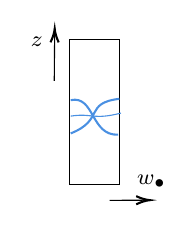
\begin{tikzpicture}[x=0.75pt,y=0.75pt,yscale=-1,xscale=1]
%uncomment if require: \path (0,300); %set diagram left start at 0, and has height of 300

%Flowchart: Process [id:dp43048504471762983] 
\draw   (257.42,59.7) -- (281.68,59.7) -- (281.68,129.5) -- (257.42,129.5) -- cycle ;
%Curve Lines [id:da4002736123725257] 
\draw [color={rgb, 255:red, 74; green, 144; blue, 226 }  ,draw opacity=1 ][line width=0.75]    (258.08,88.79) .. controls (269.74,86.33) and (267.57,105.94) .. (280.93,105.44) ;
%Curve Lines [id:da507595058105385] 
\draw [color={rgb, 255:red, 74; green, 144; blue, 226 }  ,draw opacity=1 ][line width=0.75]    (258.08,104.8) .. controls (274.5,98.34) and (264.35,90.14) .. (281.53,88.15) ;
%Curve Lines [id:da1716431524122486] 
\draw [color={rgb, 255:red, 74; green, 144; blue, 226 }  ,draw opacity=1 ]   (258.08,96.48) .. controls (268.6,94.88) and (268.54,98.51) .. (282.28,95.03) ;
%Straight Lines [id:da29626072607817044] 
\draw    (250.16,79.48) -- (250.35,56.37) ;
\draw [shift={(250.37,54.37)}, rotate = 90.48] [color={rgb, 255:red, 0; green, 0; blue, 0 }  ][line width=0.75]    (6.56,-1.97) .. controls (4.17,-0.84) and (1.99,-0.18) .. (0,0) .. controls (1.99,0.18) and (4.17,0.84) .. (6.56,1.97)   ;
%Straight Lines [id:da21464363781912077] 
\draw    (276.89,137.07) -- (294.19,136.98) ;
\draw [shift={(296.19,136.97)}, rotate = 179.7] [color={rgb, 255:red, 0; green, 0; blue, 0 }  ][line width=0.75]    (6.56,-1.97) .. controls (4.17,-0.84) and (1.99,-0.18) .. (0,0) .. controls (1.99,0.18) and (4.17,0.84) .. (6.56,1.97)   ;

% Text Node
\draw (237.62,57.13) node [anchor=north west][inner sep=0.75pt]  [font=\footnotesize] [align=left] {$\displaystyle z$};
% Text Node
\draw (288.84,123.67) node [anchor=north west][inner sep=0.75pt]  [font=\footnotesize] [align=left] {$\displaystyle w_\blt$};


\end{tikzpicture}}
	\caption{}
	\label{fig1}
\end{figure}
\end{rem}


In the following, we suppress the variable $w_\blt$ when necessary.

\begin{thm}[\textbf{Weierstrass division theorem (WDT)}]\label{lb197} \index{00@WDT: Weierstrass division theorem}
Suppose $g\in\Cbb\{w_\blt,z\}$ has order $k<\infty$ in $z$. Then for each $f\in\Cbb\{w_\blt,z\}$, there exist unique $q\in\Cbb\{w_\blt,z\}$ and $r\in\Cbb\{w_\blt\}[z]$ with degree $<k$ such that $f=gq+r$.
\end{thm}


We shall prove the Noetherian property using the following (almost) equivalent form of WDT.
\begin{thm}[\textbf{Weierstrass division theorem (WDT)}] 
Suppose $g\in\Cbb\{w_\blt,z\}=\scr O_{\Cbb^{m+1}}$ has order $k<\infty$ in $z$. Then $\scr O_{\Cbb^{m+1},0}/g\scr O_{\Cbb^{m+1},0}$ is a rank-$k$ free $\scr O_{\Cbb^m}$-module. $1,z,\dots,z^{k-1}$ are a set of free generators.
\end{thm}


\begin{thm}\label{lb70}
Every analytic local $\Cbb$-algebra $\scr O_{X,x}$ is Noetherian.
\end{thm}

\begin{proof}
It suffices to discuss $\scr O_{\Cbb^n,0}$. We prove this by induction on $n$. The case $n=0$ is trivial. Suppose the case $m=n-1$ is known. We prove the case $m+1$. We write $\scr O_m=\scr O_{\Cbb^m,0}$ and $\scr O_{m+1}=\scr O_{\Cbb^{m+1},0}$ for simplicity.
\begin{itemize}
\item Claim: If $g\in\scr O_{m+1}$ is nonzero, then $\scr O_{m+1}/g\scr O_{m+1}$ is a Noetherian ring, equivalently, a Noetherian $\scr O_{m+1}$-module.
\end{itemize}


Suppose the claim is true. Choose any non-zero ideal $I\subset\scr O_{m+1}$. Choose $0\neq g\in I$. By the claim, $I/g\scr O_{m+1}$, as a $\scr O_{m+1}$-submodule of $\scr O_{m+1}/g\scr O_{m+1}$, is $\scr O_{m+1}$-finitely generated. Thus, the exact sequence
\begin{align*}
0\rightarrow g\scr O_{m+1}\rightarrow I\rightarrow I/g\scr O_{m+1}\rightarrow0
\end{align*}
shows that $I$ is $\scr O_{m+1}$-finitely generated. This proves the case $m+1$.

It remains to prove the claim. Choose $0\neq g\in\scr O_{m+1}$. Then on a complex line passing through $0$, $0$ must be an isolated zero of $g$. (Otherwise, on each line, $g$ vanishes on a neighborhood of $0$. So $g$ vanishes on each line (and hence each domain containing $0$) by complex analysis.) By choosing new coordinates, we may assume the last coordinate axis is that line. Namely, writing $g=g(w_1,\dots,w_m,z)$, $g$ has finite order in $z$. 

By case $m$, $\scr O_m$ is Noetherian. By WDT, $\scr O_{m+1}/g\scr O_{m+1}$ is a finitely-generated $\scr O_m$-module, hence a Noetherian $\scr O_m$-module, and hence a Noetherian $\scr O_{m+1}$-module.
\end{proof}

\begin{comment}
\begin{rem}
One may compare the above proof with the proof of \textbf{Hilbert basis theorem}: if $\mc A$ is a Noetherian ring, then $\mc R=\mc A[z]$ is Noetherian.

It is not hard to see that in order to prove this theorem, it suffices to prove:
\begin{itemize}
\item Claim: If $I$ is an ideal of $\mc R$, then there exist $g_1,\dots,g_N\in I$ such that $I/\sum_{i=1}^N g_i\mc R$ is $\mc R$-finitely generated.
\end{itemize}
To prove the claim, we let $J$ be the set of leading coefficients of $\mc A$-polynomials in $\mc R$, which is clearly an ideal of $\mc A$. Since $\mc A$ is Noetherian, $J$ is finitely generated. So we can find $p_1,\dots,p_n\in I$ whose leading coefficients generate $J$. Let $r$ be the largest degree of $g_1,\dots,g_n$. Since $\mc M=\bigoplus_{j=0}^{r-1}\mc Az^j$ is a finitely-generated $\mc A$-module and hence Noetherian, $I\cap \mc M$ is $\mc A$-generated by some $g_{n+1},\dots,g_N$. Such $\{g_1,\dots,g_N\}$ makes the claim true.
\end{rem}
\end{comment}





\subsection{Proof of WDT}

We prove the first version of WDT following \cite{GR-b}.
\begin{proof}[Proof of the uniqueness]
Let $f=gq_1+r_1=gq_2+r_2$. Then $g(q_1-q_2)=r_2-r_1$. Choose a small enough neighborhood $U\times V\subset\Cbb^m\times\Cbb$ as in Rem. \ref{lb16} such that for all fixed $w_\blt\in U$, $g(z)$ has $k$ zeros in $V$ (counting multiplicities). So $g(q_1-q_2)$ has $\geq k$ zeros in $z$. Since $r_2-r_1$ has degree $<k$ in $z$, for the fixed $w_\blt$, the number of zeros of $r_2-r_1$ is either $<k$ (which is impossible), or is $\infty$. Since the latter is the only possible case, we conclude $(r_1-r_2)(z)=0$ for all $w_\blt$. And $(q_1-q_2)(z)=0$  since it is so outside the (finitely many) zeros of $g$. (One can also deduce $q_1=q_2$ from the fact that $\scr O_{\Cbb^{m+1},0}$ is an integral domain.)
\end{proof}




\begin{proof}[Discussion]
We now discuss the proof of the existence part. Let $\wht f,\wht g$ be the first $k$ terms in their power series expansions of $z$. So
\begin{gather*}
g(w_\blt,z)=\underbrace{a_0+a_1z+\cdots+a_{k-1}z^{k-1}}_{\wht g}+z^k(a_k+a_{k+1}z+a_{k+2}z^2+\cdots)
\end{gather*}
where all $a_i=a_i(w_\blt)\in\Cbb\{w_\blt\}$ and $a_0(0)=\cdots=a_{k-1}(0)=0$, $a_k(0)\neq 0$. So $(g-\wht g)z^{-k}$ and similarly $(f-\wht f)z^{-k}$ are naturally elements of $\Cbb\{w_\blt,z\}$. Moreover, $(g-\wht g)z^{-k}$ is a unit.

A na\"ive attempt to find the decomposition $f=gq+r$ is to write
\begin{align*}
f=g\cdot \frac{f-\wht f}{g}+\wht f
\end{align*}
since clearly $\wht f\in\Cbb\{w_\blt\}[z]$ has degree $<k$ in $z$. This certainly works for single-variable functions. However, when $m>0$, the expression $(f-\wht f)/g$ might not be continuous at the origin. (Take for instance the quotient to be $z^2/(wz+z^2)$.) We can only divide $f-\wht f$ by $g-\wht g$, which gives an element of $\Cbb\{w_\blt,z\}$. So we write
\begin{align*}
f=(g-\wht g)\cdot\frac{f-\wht f}{g-\wht g}+\wht f=g\cdot\frac{f-\wht f}{g-\wht g}+\wht f+\underbrace{\left(-\wht g\cdot \frac{f-\wht f}{g-\wht g}\right)}_{f_1}
\end{align*}

We then decompose $f_1$, find $f_2$, and then repeat this procedure again and again to produce an infinite series, which we hope would converge to the expected decomposition. Namely, we let $f_0=f$. So the above defines $f_1$ in terms of $f_0$. We define in a similar way $f_{n+1}$ in terms of $f_n$:
\begin{align}
f_n=g\cdot\frac{f_n-\wht f_n}{g-\wht g}+\wht f_n+f_{n+1}.\label{eq11}
\end{align}  
Substituting $f_0,f_1,\dots,f_n$ into $f$, we get
\begin{align}
&f=\left(g\cdot\frac{f_0-\wht f_0}{g-\wht g}+\wht f_0\right)+f_1\nonumber\\
=&\left(g\cdot\frac{f_0-\wht f_0}{g-\wht g}+\wht f_0\right)+\left(g\cdot\frac{f_1-\wht f_1}{g-\wht g}+\wht f_1\right)+f_2=\cdots\nonumber\\
=&g\cdot\sum_{i=0}^n\frac{f_i-\wht f_i}{g-\wht g}+\sum_{i=0}^n \wht f_i+f_{n+1}.\label{eq14}
\end{align}
In the following formal proof, we give careful analysis when $n\rightarrow\infty$.
\end{proof}





\begin{proof}[Finishing the proof of WDT]
For each $(r_\blt,\rho)=(r_1,\dots,r_m,\rho)\in\Rbb_{>0}^m\times\Rbb_{>0}$, define a norm $\lVert\cdot \lVert_{r_\blt,\rho}$ on $\Cbb\{w_\blt,z\}$ as follows: if $h=\sum_{i_1,\dots,i_m,j\in\Nbb}b_{i_\blt,j}w_1^{i_1}\cdots w_m^{i_m}z^j$ then
\begin{align*}
\lVert h\lVert_{r_\blt,\rho}=\sum_{i_1,\dots,i_m,j\in\Nbb}|b_{i_\blt,j}|r_1^{i_1}\cdots r_m^{i_m}\rho^j,
\end{align*}
which might take value $\infty$. We have
\begin{align}
\lVert h_1h_2\lVert_{r_\blt,\rho}\leq \lVert h_1\lVert_{r_\blt,\rho}\cdot\lVert h_2\lVert_{r_\blt,\rho}\qquad \lVert h-\wht h\lVert_{r_\blt,\rho}\leq \lVert h\lVert_{r_\blt,\rho}.\label{eq13}
\end{align}


We write \eqref{eq11} as
\begin{align}
-f_{n+1}=&\frac{\wht g}{(g-\wht g)}\cdot (f_n-\wht f_n)\nonumber\\
=&\frac{\wht g}{z^{-k}(g-\wht g)}\cdot z^{-k}(f_n-\wht f_n)=:\beta\cdot \alpha_n.\label{eq12}
\end{align}
By the first paragraph in the previous \textit{Discussion}, we have $\beta,\alpha_n\in\Cbb\{w_\blt,z\}$. Choose $r_\blt,\rho$ such that $f,g$ are defined (and holomorphic) and $g-\wht g$ has no zeros in the polydisc $D$ with multiradii $r_\blt,\rho$ except at the origin. Then \eqref{eq12} shows that all $f_n$ are defined in this domain.

Slightly shrink $\rho$ so that $C:=\lVert f\lVert_{r_\blt,\rho}<\infty$. \textit{Now we use the condition that $g$ has order $k$ in $z$ in full power}: it tells us that $\beta(0,z)=0$. So we may shrink $r_\blt$ such that $\lVert\beta\lVert_{r_\blt,\rho}<\frac 12\rho^k$. Clearly $\lVert f_n-\wht f_n\lVert_{r_\blt,\rho}=\rho^k\lVert\alpha_n\lVert_{r_\blt,\rho}$. So by \eqref{eq13}, 
\begin{align*}
\lVert f_{n+1}\lVert_{r_\blt,\rho}<\frac 12\lVert f_n-\wht f_n\lVert_{r_\blt,\rho}\leq \frac 12\lVert f_n\lVert_{r_\blt,\rho}.
\end{align*}
Thus $\lVert f_n\lVert_{r_\blt,\rho}< 2^{-n}C$. So $\lVert z^{-k}(f_n-\wht f_n)\lVert_{r_\blt,\rho}<2^{-n}\rho^{-k}C$ and $\lVert\wht f_n\lVert_{r_\blt,\rho}<2^{-n}C$.

The uniform norm on the polydisc with multi-radii $(r_\blt,\rho)$ is clearly $\leq \lVert\cdot\lVert_{r_\blt,\rho}$. So $f_n\rightarrow 0$ uniformly on the polydisc $D$. 
The infinite series $\sum_{i=0}^\infty\frac{z^{-k}(f_i-\wht f_i)}{z^{-k}(g-\wht g)}$ converges uniformly to a continuous function $q$ on any compact subset of $D$. $q$ is holomorphic, since it is so on each variable by Morera's theorem. Similarly, $\sum_{i=0}^\infty\wht f_i$ converges uniformly to a holomorphic $r$. Residue theorem and the fact that contour integrals commute with (uniformly convergent) infinite sum show that $r$ does not have $\geq k$ powers of $z$ (since each $\wht f_n$ does not). Thus, we obtain the decomposition $f=gq+r$ by letting $n\rightarrow\infty$ in \eqref{eq14}.
\end{proof}


\section{Germs of complex spaces}


\begin{df}
The \textbf{category of germs of complex spaces} denotes the one whose objects are $(X,x)$ where $X$ is a complex space and $x$ is a marked point. If $U\subset X$ is a neighborhood of $x$ then $(X,x)$ is identified with $(U,x)$. A \textbf{morphism of germs} from $(X,x)$ to $(Y,y)$ is a holomorphic map $\varphi:U\rightarrow Y$ where $U\subset X$ is a neighborhood of $x$ such that $\varphi(x)=y$. Two morphisms $\varphi_1,\varphi_2:(X,x)\rightarrow (Y,y)$ are regarded equal if there is a neighborhood $U$ of $x$ such that $\varphi_1|_U$ equals $\varphi_2|_U$ as holomorphic maps $U\rightarrow Y$. Composition of morphisms are the usual one for holomorphic functions (i.e. for $\Cbb$-ringed spaces). 

An \textbf{isomorphism of germs of complex spaces} $\varphi:(X,x)\rightarrow(Y,y)$ is a morphism of germs with inverses, namely, there is a morphism $\psi:(Y,y)\rightarrow (X,x)$ such that $\psi\circ\varphi$ and $\varphi\circ\psi$ are $\id$ on neighborhoods of $x$ and $y$ respectively. Equivalently, there are neighborhoods $U\ni x$ and $V\ni y$ such that $\varphi:U\rightarrow V$ is a biholomorphism, and that $\varphi(x)=y$. \hfill\qedsymbol
\end{df}




The category of analytic local $\Cbb$-algebras is understood in the obvious way: the morphisms are defined by Def. \ref{lb41}.


\begin{thm}\label{lb19}
The contravariant functor $\fk F$ from the category of germs of complex spaces to the category of analytic local $\Cbb$-algebras, sending $(X,x)$ to $\scr O_{X,x}$ and sending $\varphi:(X,y)\rightarrow(Y,y)$ to $\varphi^\#:\scr O_{Y,y}\rightarrow\scr O_{X,x}$, is an \textbf{antiequivalence of categories}. \index{00@Antiequivalence of categories} Namely:
\begin{enumerate}[label=(\arabic*)]
\item For each $(X,x)$ and $(Y,y)$, the following map is bijective
\begin{align}
\fk F:\Mor\big((X,x),(Y,y)\big)\rightarrow \Mor\big(\scr O_{Y,y},\scr O_{X,x}\big),\qquad \varphi\mapsto\varphi^\#.\label{eq15}
\end{align}
\item Each analytic local $\Cbb$-algebra is isomorphic to $\fk F((X,x))$ for some germ of complex space $(X,x)$.
\end{enumerate}
\end{thm}




Part (2) is obvious. Let us prove part (1).


\begin{proof}
Assume without loss of generality that $Y$ is a model space $\Specan(\scr O_V/\mc J)$ where $V\subset\Cbb^n$ is open and $y=0$. 

Suppose $\varphi_1^\#,\varphi_2^\#:\scr O_{Y,y}=\scr O_{\Cbb^n,0}/\mc J_0\rightarrow\scr O_{X,x}$ are equal. Then for each $j=1,\dots,n$, $\varphi_1^\#z_j$ equals $\varphi_2^\#z_j$ as elements of $\scr O_{X,x}$. So they are equal on $X$ if we shrink $X$ to a smaller neighborhood of $x$. By Thm. \ref{lb7}, $\varphi_1$ and $\varphi_2$ are equal as holomorphic maps $X\rightarrow V$, and hence are equal as $X\rightarrow Y$. So the map $\fk F$ in \eqref{eq15} is injective.

Next, we choose a morphism $\Phi:\scr O_{\Cbb^n,0}/\mc J_0\rightarrow\scr O_{X,x}$. Let $f_1=\Phi(z_1),\dots,f_n=\Phi(z_n)$, which are elements of $\scr O(X)$ if we shrink $X$ to a smaller neighborhood of $x$. View $F=(f_1,\dots,f_n)\in\scr O(X)^n$ as a holomorphic map $\varphi:X\rightarrow\Cbb^n$. Replace $X$ by $\varphi^{-1}(V)$ such that $\varphi:X\rightarrow V$. Note that $\varphi(x)=0$. So $h\in\scr O_{\Cbb^n,0}\mapsto h\circ \varphi=\varphi^\#h\in\scr O_{X,x}$ is a morphism of local $\Cbb$-algebras. It agrees with $\scr O_{\Cbb^n,0}\rightarrow\scr O_{\Cbb^n,0}/\mc J_0\xrightarrow{\Phi}\scr O_{X,x}$ on $z_1,\dots,z_n$ by the very definition of $F$. So they agree on any element of $\scr O_{\Cbb^n,0}$ due to Prop. \ref{lb8}. We conclude $\varphi^\#(h)=\Phi([h])$  for all $h\in\scr O_{\Cbb^n,0}$ (where $[h]$ denotes the residue class of $h$ in $\scr O_{\Cbb^n,0}/\mc J_0$). In particular, we have $\varphi^\#\mc J_0=0$ in $\scr O_{X,x}$.

Shrink $V$ and $X\subset\varphi^{-1}(V)$, and choose $g_1,\dots,g_k\in\scr O_{\Cbb^n}(V)$ generating the ideal $\mc J_0$ and sent by $\varphi^\#$ to $0\in\scr O(X)$. Since $\mc J$ is finite-type, by Rem. \ref{lb17}, we can shrink $V$ such that $g_1,\dots,g_k$ generate $\mc J$. Thus $\varphi^\#\mc J=0$ in $\varphi_*\scr O_X$. By Thm. \ref{lb13}, $\varphi$ restricts to a holomorphic map $\wtd\varphi:X\rightarrow Y$. $\wtd\varphi^\#:\scr O_{Y,y}=\scr O_{\Cbb^n,0}/\mc J_0\rightarrow\scr O_{X,x}$ equals $\Phi$ since $\varphi^\#:\scr O_{\Cbb^n,0}\rightarrow\scr O_{X,x}$ factors as $\scr O_{\Cbb^n,0}\rightarrow\scr O_{\Cbb^n,0}/\mc J_0\xrightarrow{\wtd\varphi^\#}\scr O_{X,x}$. This proves that $\fk F$ is surjective.
\end{proof}

\begin{co}\label{lb18}
Let $X,Y$ be complex spaces, $x\in Y,y\in Y$, and $\Phi:\scr O_{Y,y}\xrightarrow{\simeq}\scr O_{X,x}$ be an isomorphism of local $\Cbb$-algebras. Then there are neighborhoods $U\ni x,V\ni y$ and a biholomorphism $\varphi:U\xrightarrow{\simeq}V$ whose transpose $\varphi^\#:\scr O_{V,y}\rightarrow\scr O_{U,x}$ equals $\Phi$.
\end{co}

\begin{df}
An analytic local $\Cbb$-algebra is called \textbf{regular} \index{00@Recular analytic local $\Cbb$-algebras $\scr O_{\Cbb^n,0}$} if it is isomorphic to $\scr O_{\Cbb^n,0}=\Cbb\{z_1,\dots,z_n\}$ for some $n$.
\end{df}

\begin{co}\label{lb130}
Let $X$ be a complex space and $x\in X$. If $\scr O_{X,x}$ is regular, then there is a neighborhood $U$ of $x$ biholomorphic to an open subset of $\Cbb^n$ for some $n$.
\end{co}

\begin{df}\label{lb129}
We say that $X$ is \textbf{smooth at $x$} (equivalently, $x$ is a \textbf{smooth point} of $X$) if $\scr O_{X,x}$ is regular.  We say that $X$ is \textbf{smooth} (equivalently, $X$ is a complex manifold) if it is smooth everywhere. \index{00@Smooth at a point} \index{00@Smooth complex spaces=complex manifolds}
\end{df}



















\section{Immersions and closed embeddings; generating $\scr O_{X,x}$ analytically}

\begin{df}
A holomorphic map $\varphi:X\rightarrow Y$ is called an \textbf{immersion at $x\in X$} \index{00@Immersions}  if $\varphi^\#:\scr O_{Y,\varphi(y)}\rightarrow\scr O_{X,x}$ is surjective. $\varphi$ is called an \textbf{immersion} if it is an immersion at every $x\in X$. $\varphi$ is called a \textbf{closed (resp. open) embedding} if there is a commutative diagram \index{00@Closed embeddings} \index{00@Open embeddings}
\begin{equation}
\begin{tikzcd}
X \arrow[rd,"\simeq"] \arrow[rr,"\varphi"] &              & Y \\
                        & Y_0 \arrow[ru,hook,"\iota"] &  
\end{tikzcd}
\end{equation}
where $Y_0$ is a closed (resp. open) complex subspace of $Y$ and $X\xrightarrow{\simeq}Y_0$ is a biholomorphic map.
\end{df}


A closed embedding is clearly an immersion. Moreover, an immersion is locally a closed embedding:




\begin{pp}\label{lb21}
Let $\varphi:X\rightarrow Y$ be an immersion at $x$. Then there are neighborhoods $V$ of $y=\varphi(x)$ and $U\subset\varphi^{-1}(V)$ of $x$  such that $\varphi:U\rightarrow V$ is a closed embedding. In particular, $\varphi$ is an immersion on $U$.
\end{pp}




\begin{proof}
By assumption, $\varphi^\#:\scr O_{Y,y}\rightarrow\scr O_{X,x}$ is surjective. Let $J$ be its kernel, and choose generating elements $g_1,\dots,g_k\in J$. By shrinking $Y$ to a neighborhood of $y$ (and shrink $X$ accordingly), we assume $g_1,\dots,g_k\in\scr O_Y(Y)$. Let $\mc J=g_1\scr O_Y+\cdots+g_k\scr O_Y$. Then $\mc J_x=J$. Define a closed subspace $Z=\Specan(\scr O_Y/\mc J)$ of $Y$. Then $\varphi^\#$ factors as
\begin{align*}
\varphi^\#:\scr O_{Y,y}\twoheadrightarrow \scr O_{Y,y}/J=\scr O_{Z,y}\xlongrightarrow[\simeq]{\Psi}\scr O_{X,x}.
\end{align*}
By Cor. \ref{lb18}, we may shrink $X$ so that there is an open embedding $\wtd\varphi:X\rightarrow Z$, $\wtd\varphi(x)=y$, such that $\wtd\varphi^\#:\scr O_{Z,y}\rightarrow\scr O_{X,x}$ equals $\Psi$. Let $\iota:Z\rightarrow Y$ be the inclusion. Then $(\iota\wtd\varphi)^\#=\wtd\varphi^\#\iota^\#:\scr O_{Y,y}\rightarrow\scr O_{X,x}$ equals $\varphi^\#$. By Thm. \ref{lb19}, we may find open $U\ni x$  such that $\varphi=\iota\wtd\varphi$ on $U$. Since $\wtd\varphi(U)$ is an open subset of $Z$, we may find open $V\subset Y$ such that $\wtd\varphi(U)=V\cap Z=V\cap N(\mc J)$. So $\varphi$ restricts to the biholomorphism $\wtd\varphi:U\rightarrow\wtd\varphi(U)$ where $\wtd\varphi(U)$ is a closed subspace of $V$.
\end{proof}





We now discuss when an immersion is a closed embedding and give some examples.

\begin{pp}\label{lb14}
Let $X$ be complex spaces and  $\varphi:X\rightarrow Y$ a holomorphic immersion. Assume that $\varphi$ is an injective and closed map\footnote{$\varphi$ is called closed if it maps closed subsets to closed subsets.} of topological spaces. Suppose we have a finite type ideal $\mc J$ of $\scr O_Y$ such that $N(\mc J)$ equals the image of $\varphi$, and that
\begin{align}
\mc J_y=\Ker(\scr O_{Y,y}\xrightarrow{\varphi^\#}\scr O_{X,x})\label{eq9}
\end{align}
for all $x\in X$ and $y=\varphi(x)$. Then $\varphi$ is a closed embedding. More precisely, $\varphi$ restricts to a biholomorphism
\begin{align}
\wtd\varphi:X\xrightarrow{\simeq}\Specan(\scr O_Y/\mc J).\label{eq10}
\end{align}
\end{pp}

We will see in Cor. \ref{lb84} that the assumption on the existence of $\mc J$ is redundant.






\begin{proof}
Let $Y_0:=\Specan(\scr O_Y/\mc J)$. By Thm. \ref{lb13}, the restriction \eqref{eq10} as a holomorphic map exists, i.e., we have a commutative diagram
\begin{equation*}
\begin{tikzcd}
X \arrow[r, "\wtd\varphi"] \arrow[rd, "\varphi"'] & Y_0 \arrow[d, hook] \\
                                  & Y                
\end{tikzcd}
\end{equation*}
The underlying topological space of $Y_0:=\Specan(\scr O_X/\mc J)$ is $N(\mc J)$. So $\wtd\varphi$ is a continuous closed bijection from $X$ to $N(\mc J)$, which is therefore a homeomorphism. For each $x\in X,y=\varphi(x)$, the stalk map $\wtd\varphi^\#:\scr O_{Y_0,y}=\scr O_{Y,y}/\mc J_y\rightarrow\scr O_{X,x}$ is surjective since $\varphi$ is an immersion, and is injective by \eqref{eq9}. So $\wtd\varphi$ is a biholomorphism.
\end{proof}



\begin{eg}\label{lb22}
The holomorphic map $\iota:0\times\Cbb^n\rightarrow\Cbb^m\times\Cbb^n$ is an immersion and a closed injective map, and the kernels of $\iota^\#$ at the level  of stalks are the stalks of the ideal $\mc I=z_1\scr O_{\Cbb^{m+n}}+\cdots+ z_m\scr O_{\Cbb^{m+n}}$. Thus, by Prop. \ref{lb14}, $\iota$ restricts to a biholomorphism $0\times\Cbb^n\xrightarrow{\simeq}\Specan(\scr O_{\Cbb^{m+n}}/\mc I)$. This reproves Exp. \ref{lb3}.
\end{eg}



\begin{eg}\label{lb23}
Let $X$ be a complex space, and let $\mc I,\mc J$ be finite-type ideals of $\scr O_X$. Let $Y=\Specan(\scr O_X/\mc I)$. So $\scr O_Y=(\scr O_X/\mc I)|_{N(\mc I)}$. Then
\begin{align*}
\wtd {\mc J}=\big((\mc I+\mc J)/\mc I\big)\uph_{N(\mc I)}
\end{align*}
is a finite-type ideal of $\scr O_Y$, and is the unique ideal whose stalk at each $x\in N(\mc I)$ equals $(\mc I_x+\mc J_x)/\mc I_x$. Then there is a biholomorphism
\begin{align}
\Specan(\scr O_X/(\mc I+\mc J))\xlongrightarrow[\simeq]{\varphi} \Specan(\scr O_Y/\wtd{\mc J}).
\end{align}
which equals $N(\mc I+\mc J)\xrightarrow{=}N(\mc I)\cap N(\mc J)$ as maps of topological spaces, and whose stalk maps are
\begin{align*}
\scr O_{Y,x}/\wtd{\mc J}_x=\frac{\scr O_{X,x}/\mc I_x}{(\mc I_x+\mc J_x)/\mc I_x}\quad\xlongrightarrow{\simeq}\quad\scr O_{X,x}/(\mc I_x+\mc J_x).
\end{align*}
\end{eg}



\begin{proof}
The key point is to show that the above stalk isomorphisms can be assembled into a sheaf isomorphism. Consider the diagram
\begin{equation}\label{eq16}
\begin{tikzcd}
                                             & \Specan(\scr O_Y/\wtd{\mc J}) \arrow[d, hook] \\
\Specan(\scr O_X/(\mc I+\mc J)) \arrow[r, "\alpha"] \arrow[rd,hook ] \arrow[ru,"\varphi"] & Y \arrow[d, hook] \\
                                             & X                
\end{tikzcd}
\end{equation}
By Thm. \ref{lb13}, there is a holomorphic map $\alpha$ such that the lower triangle commutes. The stalk maps are $\alpha^\#:\scr O_{X,x}/\mc I_x\rightarrow\scr O_{X,x}/(\mc I_x+\mc J_x)$, with kernel $(\mc I_x+\mc J_x/\mc I_x)$. These kernels can be assembled into the ideal sheaf $\wtd{\mc J}$ on $N(\mc I)$. Thus, Prop. \ref{lb14} guarantees that there is a biholomorphism making the upper triangle in \eqref{eq16} commutes.
\end{proof}



Exp. \ref{lb23} shows that a closed complex subspace of a closed subspace is again a closed subspace of the original space. Thus, we have more generally:
\begin{co}\label{lb81}
If $\alpha:X\rightarrow Y$ and $\beta:Y\rightarrow Z$ are closed embeddings, then so is the composition $\beta\circ\alpha:X\rightarrow Z$.
\end{co}











Let us consider the special case $\varphi:X\rightarrow\Cbb^n$, where $\varphi$ is represented by $(f_1,\dots,f_n)\in\scr O_X^n$ (cf. Thm. \ref{lb7}). Then $\varphi$ is an immersion at $x$ iff the morphism of analytic local $\Cbb$-algebras  defined in Prop. \ref{lb8}, namely $\Cbb\{z_\blt\}\rightarrow\scr O_{X,x}$ sending $z_j$ to $f_j-f_j(x)$, is surjective. This actually mean that \textit{$f_1,\dots,f_n$ generate (analytically) the analytic local $\Cbb$-algebra $\scr O_{X,x}$}. (They certainly do not generate the ring $\scr O_{X,x}$ algebraically. But one can imagine that the subalgebra generated algebraically by $f_\blt$ is ``dense" in $\scr O_{X,x}$, where the density means approximation by power series of $f_1,\dots,f_n$.) The situation is similar to the case of a surjective morphism of $\Cbb$-algebras $\Cbb[z_\blt]\rightarrow A$, whose algebro-geometric meaning is that the affine scheme $\mathrm{Spec}(A)$ is embedded into the affine plane $\Cbb^n$.



We must find a criterion about whether $f_1,\dots,f_n$ generate $\scr O_{X,x}$ (analytically). At first sight, this problem seems not easy even if $X$ is smooth. (For instance, take $f_1,\dots,f_n$ to be some arbitrary holomorphic functions and deduce whether they generate $\scr O_{X,x}$.) There is indeed a simple criterion, which is proved using the (holomorphic version of) inverse function theorem. To begin with, we define:
\begin{df}
If $X$ is a complex space and $x\in X$, the vector space $\fk m_{X,x}/\fk m_{X,x}^2$ is called the \textbf{cotangent space}  of $X$ at $x$, and its dual space $(\fk m_x/\fk m_x^2)^*$ is called the \textbf{tangent space}.\index{00@Cotangent space $\fk m_x/\fk m_x^2$ and tangent space $(\fk m_x/\fk m_x^2)^*$} Since $\scr O_{X,x}$ is Noetherian, $\fk m_{X,x}$ is finitely-generated, and hence $\fk m_{X,x}/\fk m_{X,x}^2$ is finite-dimensional.
\end{df}

It is inspiring to write the residue class of $f-f(x)$ (where $f\in\scr O(X)$) in the cotangent space $\fk m_{X,x}/\fk m_{X,x}^2$ as $d_xf$.





\begin{thm}\label{lb25}
Let $X$ be a complex space and $x\in X$. Let $f_1,\dots,f_n\in\scr O(X)$. Consider $(f_1,\dots,f_n)$ as a holomorphic map $\varphi:X\rightarrow\Cbb^n$ (cf. Thm. \ref{lb7}). The following are equivalent.
\begin{enumerate}[label=(\arabic*)]
\item $\varphi$ is an immersion at $x$.
\item The morphism of analytic local $\Cbb$-algebras $\Phi:\scr O_{\Cbb^n,\varphi(x)}\rightarrow\scr O_{X,x}$ sending each $z_i$ to $f_i$ (cf. Prop. \ref{lb8}) is surjective. 
\item (The residue classes of) $f_1-f_1(x),\dots,f_n-f_n(x)$ span $\fk m_{X,x}/\fk m_{X,x}^2$.
\item (The germs of) $f_1-f_1(x),\dots,f_n-f_n(x)$ generate the ideal $\fk m_{X,x}$.
\end{enumerate}
If any of these conditions holds, we say that $f_1,\dots,f_n$ \textbf{generate (the algebra) $\scr O_{X,x}$ analytically}. \index{00@Analytically generating $\scr O_{X,x}$}
\end{thm}

\begin{proof}
Assume for simplicity that $\varphi(x)=0$. Clearly (1)$\Leftrightarrow$(2) and (3)$\Leftrightarrow$(4). (Note that (3)$\Rightarrow$(4) follows from Nakayama's lemma.) It remains to prove (2)$\Leftrightarrow$(3). 

Assume (2). Choose any $g\in\fk m_{X,x}$. Then there is $h(z_\blt)\in\scr O_{\Cbb^n,0}$ sent by $\Phi$ to $g$. We may write $h(z_\blt)=\sum_i a_iz_i+\text{an element of }\fk m_{\Cbb^n,0}^2$ where $a_i\in\Cbb$. Since $\Phi(z_i)=f_i$ and $\Phi(\fk m_{\Cbb}^2)\subset\fk m_{X,x}^2$, we have $g\in \sum_i a_i f_i+\fk m_{X,x}^2$. This proves (3).

Asume (3). By discarding some elements, we may assume that $f_1,\dots,f_n$ form a basis of $\fk m_{X,x}/\fk m_{X,x}^2$. Assume $X$ is a model space $\Specan(\scr O_U/\mc I)$ where $U\subset\Cbb^N$ is open and $x=0$. So $\scr O_{X,x}=\scr O_{\Cbb^N,0}/\mc I_0$, $\fk m_{X,x}=\fk m_{\Cbb^N,0}/\mc I_0$, and hence
\begin{align}
\fk m_{X,x}/\fk m_{X,x}^2=\fk m_{\Cbb^N,0}/(\fk m_{\Cbb^N,0}^2+\mc I_0).\label{eq60}
\end{align}
Lift $f_\blt$ to elements of $\scr O_{\Cbb^N,0}$, still denoted by $f_\blt$. Then we can extend $f_1,\dots,f_n$ to a list $f_1,\dots,f_N$ whose residue classes form a basis of $\fk m_{\Cbb^N,0}/\fk m_{\Cbb^N,0}^2$ such that $f_{n+1},\dots,f_N\in\mc I_0$. By the inverse function theorem, we may assume $x=0$ and $f_1,\dots,f_N$ are the standard coordinates $z_1,\dots,z_N$ of $\Cbb^N$. By shrinking $U$, we may assume $z_{n+1},\dots,z_N\in\mc I(U)$.

Assume for simplicity that $\mc I$ is generated by $z_{n+1},\dots,z_N$ together with $g_1,\dots,g_k\in\mc I(U)$. Let $\mc I_1=z_{n+1}\scr O_U+\cdots+z_N\scr O_U$. Then by Exp. \ref{lb23}, $X=\Specan(\scr O_U/\mc I)$ is naturally a closed subspace of $X_1=\Specan(\scr O_U/\mc I_1)$ (defined by $g_1,\dots,g_k$). By Exp. \ref{lb22}, $X_1$ is naturally equivalent to $U\cap(\Cbb^n\times 0)$. So the map $(z_1,\dots,z_n):X_1\rightarrow \Cbb^n$ is an open embedding. $\varphi$ is its restriction to $X$, which is therefore an immersion at $0$. This proves (1) and hence (2).
\end{proof}



\begin{rem}\label{lb191}
Assume that $X,Y$ are complex manifolds and $\varphi:X\rightarrow Y$ is a closed embedding of complex spaces. Let $x\in X$. Then by Thm. \ref{lb25},  $\varphi$ is an immersion at $x$ in the sense of complex differential manifolds, namely, it induces an injective map of tangent spaces (since its transpose is a surjective map of cotangent spaces). Therefore, since $\varphi$ is also a homeomorphism from $X$ to its image in $Y$, as in the case of real differential manifolds, one can use inverse function theorem to find a neighborhood $V$ of $y=\varphi(x)$, a  biholomorphic map $\beta$ from $V$ to a neighborhood $\wtd V$ of $0\in\Cbb^n$, and biholomorphism $\alpha$ from $U=\varphi^{-1}(V)$ to a neighborhood $\wtd U$ of $0\in\Cbb^m$ (where $m\leq n$), such that $\beta\circ\varphi\circ\alpha^{-1}:\wtd U\rightarrow\wtd V$ is the restriction of the closed embedding $\Cbb^m\simeq\Cbb^m\times\{0\}\hookrightarrow\Cbb^m\times\Cbb^{n-m}$.
\end{rem}



We give an application of analytically generating elements.


\begin{pp}\label{lb24}

\item Let $\Phi,\Psi:\scr O_{Y,y}\rightarrow\scr O_{X,x}$ be morphisms of analytic local $\Cbb$-algebras. Assume $f_1,\dots,f_n\in\scr O_{Y,y}$ generate the algebra $\scr O_{Y,y}$ analytically. 
\begin{enumerate}[label=(\arabic*)]
\item If $\Phi(f_i)=\Psi(f_i)$ for all $i=1,\dots,n$, then $\Phi=\Psi$.
\item Let $I$ be the ideal of $\scr O_{X,x}$ generated by $\Phi(f_i)-\Psi(f_i)$ for all $i$. Then $I$ contains $\Phi(h)-\Psi(h)$ for every $h\in\scr O_{Y,y}$.
\end{enumerate}
\end{pp}

\begin{proof}
(1): By Prop. \ref{lb8}, we have a (unique) morphism $\Upsilon:\scr O_{\Cbb^n,0}\rightarrow\scr O_{Y,y}$ sending $z_i$ to $f_i-f_i(x)$. So $\Phi\circ\Upsilon$ and $\Psi\circ\Upsilon$ agree at $z_1,\dots,z_n$. So $\Phi\circ\Upsilon=\Psi\circ\Upsilon$ by Prop. \ref{lb8}. By assumption, $\Upsilon$ is surjective. So $\Phi=\Psi$. 

(2): Apply (1) to the restriction $\Phi,\Psi:\scr O_{Y,y}\rightarrow\scr O_{X,x}/I$.
\end{proof}


Prop. \ref{lb24}-(2) is the stalk version of a geometric construction called equalizer.


\section{Equalizers of $X\rightrightarrows Y$}

\begin{df}\label{lb139}
Let $\varphi,\psi:X\rightarrow Y$ be holomorphic maps of complex spaces. A \index{00@Equalizers} \textbf{kernel} or an \textbf{equalizer of the double arrow} $\begin{tikzcd}
X \arrow[r,shift left, "\varphi"] \arrow[r,shift right,"\psi"'] & Y
\end{tikzcd}$
is a complex space $E$ and a holomorphic map $\iota:E\rightarrow X$ such that $\varphi\circ\iota=\psi\circ\iota$, and that for every complex space $S$ and holomorphic map $\mu:S\rightarrow X$ satisfying $\varphi\circ\mu=\psi\circ\mu$ there is a unique holomorphic $\wtd\mu:S\rightarrow E$ such that $\mu=\iota\circ\wtd\mu$.
\begin{equation}\label{eq17}
\begin{tikzcd}
S \arrow[rd, "\mu"] \arrow[d, "{\wtd\mu}"', dashed] &                                                           &   \\
E \arrow[r, "\iota"']                   & X \arrow[r, "\psi"', shift right] \arrow[r, "\varphi", shift left] & Y
\end{tikzcd}
\end{equation}
It is easy to see that equalizers are unique up to isomorphisms.
\end{df}

The main result of this section is:

\begin{thm}\label{lb26}
Every double arrow $\begin{tikzcd}
X \arrow[r,shift left, "\varphi"] \arrow[r,shift right,"\psi"'] & Y
\end{tikzcd}$ of holomorphic maps has an equalizer which is the inclusion map of a closed subspace $\iota:E=\Specan(\scr O_X/\mc I)\hookrightarrow X$. This is called the \textbf{canonical equalizer}. \index{00@Canonical equalizers} The finite-type ideal $\mc I$ is uniquely determined by the fact that for all $x\in X$:
\begin{enumerate}[label=(\alph*)]
\item If $\varphi(x)\neq\psi(x)$, then $\mc I_x=\scr O_{X,x}$.
\item If $\varphi(x)=\psi(x)$, then by considering $\varphi^\#,\psi^\#$ as stalk maps $\scr O_{Y,\varphi(x)}\rightarrow\scr O_{X,x}$, $\mc I_x$ is the ideal of $\scr O_{X,x}$ generated by all $\varphi^\#(f)-\psi^\#(f)$ (where $f\in\scr O_{Y,\varphi(x)}$).
\end{enumerate}
Moreover, $N(\mc I)$, the underlying set of $E$, is $\Delta=\{x\in X:\varphi(x)=\psi(x)\}$.
\end{thm}

From Prop. \ref{lb24}, it is clear that $\mc I_x$ is generated by $\varphi^\#(f_i)-\psi^\#(f_i)$ if $f_1,\dots,f_n\in\scr O_{Y,y}$ generate the algebra $\scr O_{Y,y}$ analytically, e.g. $z_1,\dots,z_n$ if $Y$ is a model space in $\Cbb^n$.

\begin{rem}\label{lb42}
From Thm. \ref{lb26}, it is clear that if $E_0\rightarrow X$ is an equalizer of $X\rightrightarrows Y$, then it is a closed embedding, and equals the composition of a unique biholomorphism $E_0\xrightarrow{\simeq} E$ and the inclusion map $E\hookrightarrow X$ where $E$ is the canonical equalizer.
\end{rem}



\begin{proof}[Construction of $E$]
We define a finite-type ideal $\mc I$ satisfying (a) and (b). We shall first define it locally and then glue the pieces. Then $\mc I$ gives $E$.

Let $\Omega=X\setminus \Delta$ which is open.  We set $\mc I_\Omega=\scr O_X|_\Omega$. For each $x\in \Delta$, we choose a neighborhood $V_y\subset Y$ of $y=\varphi(x)$ biholomorphic to a model space. So we can choose finitely many $f_1,\dots f_n\in\scr O_Y(V_y)$ embedding $V_y$ onto a closed subspace of an open subset of $\Cbb^n$. $U_x=\varphi^{-1}(V_y)\cap \psi^{-1}(V_y)$ is a neighborhood of $x$, and we set $\mc I_{U_x}$ to be the ideal of $\scr O_{U_x}$ generated by $\varphi^\#(f_1)-\psi^\#(f_1),\dots,\varphi^\#(f_n)-\psi^\#(f_n)$ (defined on $U_x$).

We claim that these locally defined finitely-generated ideals are compatible. If $p\in U_x\cap \Delta$ then, as $\varphi(p)=\psi(p)$, by Prop. \ref{lb24} or by substitution rule (Rem. \ref{lb27}), the stalk $(\mc I_{U_x})_p$ is the ideal generated by all $\varphi^\#(f)-\psi^\#(f)\in\scr O_{X,p}$ where $f\in\scr O_{Y,\varphi(p)}$. If $p\in U_x\cap\Omega$, then as $\varphi(p)\neq\psi(p)$ and $(f_1,\dots,f_n)$ is an embedding, there is some $f_i$ among $f_1,\dots,f_n$ such that $\varphi^\#(f_i)-\psi^\#(f_i)$ has non-zero value at $p$, and hence its germ at $p$ is not in $\fk m_{X,p}$. This proves $(\mc I_{U_x})_p=\scr O_{X,p}$. Combining these two cases together, we see that $\mc I_\Omega$ and $\mc I_{U_x}$ (for all $x\in\Delta$) are compatible. This defines $\mc I$.

If $\varphi(x)\neq\psi(x)$, then $\mc I_x=\scr O_{X,x}$ shows $x\notin N(\mc I)$. If $\varphi(x)=\psi(x)$, then $\varphi^\#(f)-\psi^\#(f)$ vanishes at $x$ by \eqref{eq8}. So $\mc I_x$ vanishes at $x$. So $x\in N(\mc I)$. This proves $\Delta=N(\mc I)$.
\end{proof}



\begin{proof}[Proof that $E$ is an equalizer]
It is easy to check $\varphi\circ\iota=\psi\circ\iota$. Choose any holomorphic $\mu:S\rightarrow X$ such that $\varphi\circ\mu=\psi\circ\mu$. For any $s\in S$, let $x=\mu(s)$. Then $\varphi(x)=\psi(x)$. Choose any $f\in\scr O_{Y,\varphi(x)}$. Then $\varphi\circ\mu=\psi\circ\mu$ shows that $\mu^\#$ sends $\varphi^\#(f)-\psi^\#(f)$ to $0\in\scr O_{S,s}$. Thus $\mu^\#:\scr O_{X,x}\rightarrow\scr O_{S,s}$ vanishes on $\mc I_x$. Thus, by Thm. \ref{lb13}, there is a unique holomorphic $\wtd\mu:S\rightarrow E$ such that the triangle in \eqref{eq17} commutes.
\end{proof}
The proof of Thm. \ref{lb26} is finished. From the proof, we know:


\begin{rem}\label{lb38}
Assume the setting of Thm. \ref{lb26}. Assume $\varphi(x)=\psi(x)=:y$. Let $V_y$ be a neighborhood of $y$ biholomorphic to a model space. More precisely, we choose $(f_1,\dots,f_n)\in\scr O_Y(V_y)^n$ which, considered as a holomorphic map $V_y\rightarrow\Cbb^n$, is a closed embedding of $V_y$ into an open subset of $\Cbb^n$. Let $U_x=\varphi^{-1}(V_y)\cap\psi^{-1}(V_y)$. Then the ideal sheaf $\mc I|_{U_x}$ is generated by $\varphi^\#(f_1)-\psi^\#(f_1),\dots,\varphi^\#(f_n)-\psi^\#(f_n)\in\scr O(U_x)$.
\end{rem}




















\section{$\scr E\otimes_{\scr O_X}\scr F$, $\Hom_{\scr O_X}(\scr E,\scr F)$, and $\shom_{\scr O_X}(\scr E,\scr F)$ }


We fix a $\Cbb$-ringed space $X$. 

\subsection{Tensor product}



\begin{df}
Let $\scr E$ and $\scr F$ be $\scr O_X$-modules. Consider the presheaf $\scr G$ of $\scr O_X$-modules defined by $\scr G(U)=\scr E(U)\otimes_{\scr O(U)}\scr F(U)$. The tensor product of restriction maps $\scr E(U)\rightarrow\scr E(V)$ and $\scr F(U)\rightarrow\scr F(V)$ gives the restriction map $\scr G(U)\rightarrow\scr G(V)$. The sheafification of $\scr G$ is denoted by $\scr E\otimes_{\scr O_X}\scr F$ or simply $\scr E\otimes\scr F$ \index{00@Tensor product $\scr E\otimes_{\scr O_X}\scr F$} and called the \textbf{tensor product} of $\scr E$ and $\scr F$.
\end{df}



\begin{rem}\label{lb258}
Let $A$ be a commutative ring, and fix an $A$-module $\mc N$. Recall the following basic facts:
\begin{enumerate}[label=\arabic*.]
\item \textbf{Tensor products commute with direct limits}. More precisely, let $(\mc M_\alpha)$ be a direct system of $A$-modules. Then the canonical map $\mc M_\beta\otimes_A\mc N\rightarrow(\varinjlim_\alpha \mc M_\alpha)\otimes_A\mc N$ (for each fixed $\beta$) defines, by passing to the direct limit, an isomorphism
\begin{align}
\varinjlim_\alpha (\mc M_\alpha\otimes_A\mc N)\xrightarrow{\simeq} (\varinjlim_\alpha \mc M_\alpha)\otimes_A\mc N.
\end{align}
(Proof: Construct the inverse map explicitly.)
\item \textbf{The tensor product functor $-\otimes\mc N$ is right exact}. \index{00@Right exact} Namely, if
\begin{align*}
\mc M_1\xrightarrow{f}\mc M_2\xrightarrow{g}\mc M_3\rightarrow0
\end{align*}
is an exact sequence of $A$-modules, then so is
\begin{align*}
\mc M_1\otimes\mc N\xrightarrow{f\otimes\id}\mc M_2\otimes\mc N\xrightarrow{g\otimes\id}\mc M_3\otimes\mc N\rightarrow 0.
\end{align*}
Identify $\mc M_3$ with $\Cok f=\mc M_2/f(\mc M_1)$. Then the right exactness of tensor product is equivalent to that \textbf{tensor products commute with cokernels}: we have an equivalence of $A$-modules
\begin{align}
\Cok\big(\mc M_1\otimes_A\mc N\xrightarrow{f\otimes\id}\mc M_2\otimes_A\mc N \big)\quad\xlongrightarrow{\simeq}\quad \Cok\big(\mc M_1\xrightarrow{f}\mc M_2\big)\otimes_A\mc N\label{eq1}
\end{align}
descended from the canonical morphism
\begin{align}
\mc M_2\otimes_A\mc N\longrightarrow \frac{\mc M_2}{f(\mc M_1)}\otimes_A\mc N.
\end{align}
\end{enumerate}
\hfill\qedsymbol
\end{rem}

\begin{proof}
We have a well-defined map sending $\frac{\mc M_2}{f(\mc M_1)}\times\mc N$ to $\frac{\mc M_2\otimes_A\mc N}{(f\otimes\id)(\mc M_1\otimes_A\mc N)}$ (i.e. the LHS of \eqref{eq1}) sending $[\xi]\times\eta$ to $[\xi\otimes_A\eta]$, where $[\cdots]$ stands for the residue classes, and $\xi\in\mc M_2,\eta\in\mc N$. This map is clearly $A$-biinvariant. So it gives an $A$-module morphism from the RHS to the LHS of \eqref{eq1}, which is clearly the inverse of the map in \eqref{eq1} from LHS to RHS. So \eqref{eq1} is an isomorphism.
\end{proof}




\begin{rem}\label{lb4}
We can now use \eqref{eq1} to explain the last equality of \eqref{eq5}:
\begin{align*}
&\scr E_x\otimes_{\scr O_{X,x}}(\scr O_{X,x}/\fk m_x)=\scr E_x\otimes \Cok(\fk m_x\hookrightarrow \scr O_{X,x})\\
\simeq&\Cok(\scr E_x\otimes\fk m_x\rightarrow \scr E_x\otimes\scr O_{X,x})\simeq\Cok(\scr E_x\otimes\fk m_x\rightarrow \scr E_x)=\scr E_x/{\fk m_x\scr E_x}
\end{align*}
since the image of the multiplication map $\scr E_x\otimes\fk m_x\rightarrow \scr E_x$ is $\fk m_x\scr E_x$.
\end{rem}


\begin{pp}
The canonical morphism of $\scr O(U)$-modules
\begin{align*}
\scr E(U)\otimes_{\scr O(U)}\scr F(U)\rightarrow\scr E_x\otimes_{\scr O_{X,x}}\scr F_x
\end{align*}
(where $U\ni x$ is open and the map is the tensor product of $\scr E(U)\rightarrow\scr E_x$ and $\scr F(U)\rightarrow\scr F_x$) induces an isomorphism
\begin{align}
(\scr E\otimes\scr F)_x=\varinjlim_{U\ni x}\scr E(U)\otimes_{\scr O(U)}\scr F(U)\quad\xlongrightarrow{\simeq}\quad\scr E_x\otimes_{\scr O_{X,x}}\scr F_x.\label{eq2}
\end{align}
\end{pp}
\begin{proof}
Define a canonical map from $\scr E_x\times\scr F_x$ to $\varinjlim_{U\ni x}\scr E(U)\otimes_{\scr O(U)}\scr F(U)$ and show that it is $\scr O_{X,x}$-biinvariant.  This descends to the inverse map of \eqref{eq2}.
\end{proof}

\begin{co}\label{lb44}
For each $\scr O_X$-module $\scr F$, the functor $-\otimes\scr F$ on the abelian category of $\scr O_X$-modules is right exact: if
\begin{align*}
\scr E_1\rightarrow\scr E_2\rightarrow\scr E_3\rightarrow 0
\end{align*}
is exact, then so is
\begin{align*}
\scr E_1\otimes\scr F\rightarrow\scr E_2\otimes\scr F\rightarrow\scr E_3\otimes\scr F\rightarrow 0.
\end{align*}
\end{co}

\begin{proof}
Exactness of sheaves can be checked at the level of stalks. Then this follows from the isomorphism \eqref{eq2} and the right exactness of $-\otimes_{\scr O_{X,x}}\scr F_x$.
\end{proof}


\subsection{Hom}

We leave it to the readers to check the following easy facts:
\begin{rem}\label{lb51}
Let $A$ be a commutative ring, and fix an $A$-module $\mc N$:
\begin{enumerate}[label=\arabic*.]
\item \textbf{$\Hom_A(\mc N,-)$ is a left exact functor}. \index{00@Left exact (contravarient) functor} Namely, for any exact sequence of $A$-modules
\begin{align}
0\rightarrow\mc M_1\xrightarrow{f} \mc M_2\xrightarrow{g}\mc M_3,
\end{align}
we have an exact sequence 
\begin{align*}
0\rightarrow\Hom_A(\mc N,\mc M_1)\xrightarrow{f_*} \Hom_A(\mc N,\mc M_2)\xrightarrow{g_*}\Hom_A(\mc N,\mc M_3)
\end{align*}
where $f_*$ sends $T$ to $f\circ T$ and $g_*$ is defined similarly. Equivalently, \textbf{$\Hom_A(\mc N,-)$ commutes with kernels}: there is a equivalence
\begin{align}
\Hom_A\big(\mc N,\Ker(\mc M_2\xrightarrow{g}\mc M_3)\big)\simeq \Ker \big(\Hom_A(\mc N,\mc M_2)\xrightarrow{g_*}\Hom_A(\mc N,\mc M_3)\big)
\end{align}
induced by the obvious inclusion
\begin{align*}
\Hom_A\big(\mc N,\Ker(\mc M_2\xrightarrow{g}\mc M_3)\big)\hookrightarrow\Hom_A(\mc N,\mc M_2).
\end{align*}
\item \textbf{$\Hom_A(-,\mc N)$ is a left exact contravariant functor}. \index{00@Left exact (contravarient) functor} for any exact sequence of $A$-modules
\begin{align}
\mc M_1\xrightarrow{f} \mc M_2\xrightarrow{g}\mc M_3\rightarrow 0
\end{align}
we have an exact sequence 
\begin{align*}
0\rightarrow\Hom_A(\mc M_3,\mc N)\xrightarrow{g^*} \Hom_A(\mc M_2,\mc N)\xrightarrow{f^*}\Hom_A(\mc M_1,\mc N)
\end{align*}
where $f^*$ sends $T$ to $T\circ f$ and $g^*$ is defined similarly. Equivalently, \textbf{$\Hom_A(-,\mc N)$ turns cokernels into kernels}: there is a canonical equivalence
\begin{align}
\Hom_A\big(\Cok(\mc M_1\xrightarrow{f}\mc M_2),\mc N\big)\simeq \Ker \big(\Hom_A(\mc M_2,\mc N)\xrightarrow{f^*}\Hom_A(\mc M_1,\mc N)\big)
\end{align}
induced by the obvious inclusion
\begin{align*}
\Hom_A\big(\Cok(\mc M_1\xrightarrow{f}\mc M_2),\mc N\big)\hookrightarrow\Hom_A(\mc M_2,\mc N).
\end{align*}
\end{enumerate}
\end{rem}



\begin{df}
Let $\scr E,\scr F$ be $\scr O_X$-modules.  The \textbf{hom space} $\Hom_{\scr O_X}(\scr E,\scr F)$ is defined to be the space of all $\scr O_X$-module morphims from $\scr E$ to $\scr F$. \index{Hom@$\Hom_{\scr O_X}(\scr E,\scr F)$, $\shom_{\scr O_X}(\scr E,\scr F)$} 

The presheaf of $\scr O_X$-modules sending each open $U\subset X$ to the $\scr O(U)$-module $\Hom_{\scr O_U}(\scr E_U,\scr F_U)$, and whose restriction map is the obvious restriction of sheaf morphisms, is automatically a sheaf of $\scr O_X$-modules. It is called the \textbf{hom sheaf} and denoted by  $\shom_{\scr O_X}(\scr E,\scr F)$.

The dual and the double dual of $\scr E$ is defined by \index{00@Dual sheaf $\scr E^\vee$}
\begin{gather}
\scr E^\vee=\shom_{\scr O_X}(\scr E,\scr O_X),\qquad \scr E^{\vee\vee}=(\scr E^\vee)^\vee.
\end{gather}
\hfill\qedsymbol
\end{df}

\begin{exe}
Describe canonical equivalences
\begin{align}
\scr E\simeq\scr E\otimes_{\scr O_X}\scr O_X\simeq\scr O_X\otimes_{\scr O_X}\scr E\simeq \shom_{\scr O_X}(\scr O_X,\scr E).
\end{align}
\end{exe}

In general, the stalks of $\shom_{\scr O_X}(\scr E,\scr F)$ cannot be identified with $\Hom_{\scr O_{X,x}}(\scr E_x,\scr F_x)$. But good things happen when $\scr E$ is coherent, as we will see in Cor. \ref{lb50}.



\section{$(\scr O_X\mathrm{-mod})\otimes_{\scr O_S}(\scr O_S\mathrm{-mod})$; pullback sheaves}


\begin{df}
Let $\varphi:X\rightarrow S$ be a holomorphic map of complex spaces. Let $\scr E$ be an $\scr O_X$-module and $\scr M$ an $\scr O_S$-module. Then $\scr E\otimes_{\scr O_S}\scr M=\scr M\otimes_{\scr O_S}\scr E$ \index{00@Tensor product $\scr E\otimes_{\scr O_S}\scr M\simeq \scr E\otimes_{\scr O_X}\varphi^*\scr M$} denotes the sheafification of the presheaf of $\scr O_X$-modules sending each open $U\subset X$ to
\begin{align}
(\scr E\otimes_{\scr O_S}\scr M)^\pre(U)=\varinjlim_{V\supset\varphi(U)}\scr E(U)\otimes_{\scr O_S(V)}\scr M(V)
\end{align}
where the direct limit is over all open subset $V\subset S$ containing $\varphi(U)$, and $g\in\scr O_S(V)$ acts on $\sgm\in\scr E(U)$ as
\begin{align}
g\cdot \sgm:=\varphi^\#(g)\cdot \sgm.\label{eq19}
\end{align}
For each $x\in X$, we have a canonical equivalence
\begin{align}
(\scr E\otimes_{\scr O_S}\scr M)_x\simeq\scr E_x\otimes_{\scr O_{S,\varphi(x)}}\scr M_{\varphi(x)}.
\end{align}
Thus $\scr M\mapsto \scr E\otimes_{\scr O_S}\scr M$ and $\scr E\mapsto \scr E\otimes_{\scr O_S}\scr M$ are right exact functors.
\end{df}

\begin{df}\label{lb336}
The \textbf{pullback sheaf} of $\scr M$ along $\varphi$ is the $\scr O_X$-module defined by \index{00@Pullback sheaf $\varphi^*\scr M$, pullback of sections  and morphisms}
\begin{align}
\varphi^*\scr M:=\scr O_X\otimes_{\scr O_S}\scr M
\end{align} 
whose stalk at $x$ is $\scr O_{X,x}\otimes_{\scr O_{S,\varphi(x)}}\scr M_x$. It can be viewed as the induced representation of $\scr M$. Thus we may write
\begin{align}
\scr E\otimes_{\scr O_S}\scr M=\scr E\otimes_{\scr O_X}\varphi^*\scr M.
\end{align}
If $V\subset S$ is open and $\sigma\in\scr M(V)$, then the \textbf{pullback section} $\varphi^*(\sigma)\in\varphi^*\scr M(\varphi^{-1}(V))$ is the image of
\begin{align}
1\otimes \sigma\in\scr O(\varphi^{-1}(V))\otimes_{\scr O(V)}\scr M(V)\rightarrow(\scr O_X\otimes_{\scr O_S}\scr M)(\varphi^{-1}(V))=(\varphi_*\varphi^*\scr M)(V).
\end{align}
This gives a canonical morphism of $\scr O_S$-modules
\begin{align}
\scr M\rightarrow\varphi_*\varphi^*\scr M.
\end{align}


If $g:\scr M_1\rightarrow\scr M_2$ is a morphism of $\scr O_S$-modules, we define an $\scr O_X$-module morphism
\begin{align}
\varphi^*g:=\id\otimes g:\scr O_X\otimes_{\scr O_X}\scr M_1\rightarrow\scr O_X\otimes_{\scr O_X}\scr M_2,
\end{align}
called the \textbf{pullback of $g$}. %If $\sigma\in\scr M_1(V)$, then
%\begin{align}
%\varphi^*g(\varphi^*\sigma)=\varphi^*(g(\sigma))\qquad\in\scr M_2(\varphi^{-1}(V)).
%\end{align}
%\hfill\qedsymbol
\end{df}

The notation $\scr E\otimes_{\scr O_S}\scr M$ is a generalization of $\scr E\otimes_\Cbb W$ for a ($\Cbb$-)vector space $W$ by viewing $\Cbb$ as the structure sheaf of the single reduced point $\{0\}$, and by viewing the holomorphic map as the obvious one $X\rightarrow\{0\}$.



\begin{pp}\label{lb337}
$(\varphi^*,\varphi_*)$ is a pair of \textbf{adjoint functors} between the categories of $\scr O_X$-modules and $\scr O_S$-modules \index{00@Adjoint functors} (with $\varphi^*$ the left adjoint and $\varphi_*$ the right one). Namely, there is a natural isomphism
\begin{align}
\Hom_{\scr O_X}(\varphi^*\scr M,\scr E)\xrightarrow{\simeq}\Hom_{\scr O_S}(\scr M,\varphi_*\scr E).
\end{align}
The word \textbf{natural} \index{00@Natural morphisms} means that for any morphisms $g:\scr M_2\rightarrow\scr M_1$ of $\scr O_S$-modules and $f:\scr E_1\rightarrow\scr E_2$ of $\scr O_X$-modules, $\varphi^*g$ and $\varphi_*f$ induce a commutative diagram
\begin{equation}
\begin{tikzcd}
\Hom_{\scr O_X}(\varphi^*\scr M_1,\scr E_1) \arrow[d] \arrow[r,"\simeq"] & \Hom_{\scr O_S}(\scr M_1,\varphi_*\scr E_1) \arrow[d] \\
\Hom_{\scr O_X}(\varphi^*\scr M_2,\scr E_2) \arrow[r,"\simeq"]           & \Hom_{\scr O_S}(\scr M_2,\varphi_*\scr E_2)          
\end{tikzcd}
\end{equation}
\end{pp}

\begin{proof}
Given a morphism $F:\varphi^*\scr M\rightarrow\scr E$, the composition of $\scr M\rightarrow\varphi_*\varphi^*\scr M$ with $\varphi_*F:\varphi_*\varphi^*\scr M\rightarrow\varphi_*\scr E$ gives a morphism $G:\scr M\rightarrow\varphi_*\scr E$. Informally,
\begin{align}
G(\sigma)=F(1\otimes\sigma).
\end{align}
We leave it to the readers to check that $F\mapsto G$ is natural.

Conversely, given $G:\scr M\rightarrow\varphi_*\scr E$. The $\scr O(U)$-module morphisms
\begin{gather*}
\scr O(U)\otimes_{\scr O(V)}\scr M(V)\rightarrow\scr E(U),\qquad f\otimes\sigma\mapsto f\cdot G(\sigma)|_U
\end{gather*}
for all open $U\subset X$ and $V\supset \varphi(U)$ pass to $F:\varphi^*\scr M\rightarrow\scr E$. This gives the inverse of the above construction.
\end{proof}

\begin{pp}\label{lb415}
Let $\varphi:X\rightarrow S$ be a holomorphic map of complex spaces. Let $\scr E$ and $\scr F$ be $\scr O_S$-modules. Then we have a canonical isomorphism of $\scr O_X$-modules
\begin{align}\label{eq221}
\varphi^*(\scr E\otimes_{\scr O_S}\scr F)\xlongrightarrow{\simeq}\varphi^*\scr E\otimes_{\scr O_X}\varphi^*\scr F
\end{align}
\end{pp}

\begin{proof}
The $\scr O(V)$-module morphisms
\begin{gather*}
\scr E(V)\otimes_{\scr O(V)}\scr F(V)\rightarrow \varphi^*\scr E(\varphi^{-1}(V))\otimes_{\scr O(\varphi^{-1}(V))}\varphi^*\scr F(\varphi^{-1}(V))\\
\sgm\otimes\sigma\mapsto \varphi^*(\sgm)\otimes\varphi^*(\sigma)
\end{gather*}
(for all open $V\subset S$) pass to a morphism $\scr E\otimes_{\scr O_S}\scr F\rightarrow \varphi_*(\varphi^*\scr E\otimes_{\scr O_X}\varphi^*\scr F)$, and hence, by Prop. \ref{lb337}, a morphism \eqref{eq221}. Its stalk map at each $x\in X$ is (setting $t=\varphi(x)$) the canonical morphism
\begin{align*}
(\scr E_t\otimes_{\scr O_{S,t}}\scr F_t)\otimes_{\scr O_{S,t}}\scr O_{X,x}\rightarrow(\scr E_t\otimes_{\scr O_{S,t}}\scr O_{X,t})\otimes_{\scr O_{X,x}}(\scr F_t\otimes_{\scr O_{S,t}}\scr O_{X,t})
\end{align*}
which is an isomorphism by Lem. \ref{lb408}.
\end{proof}




\begin{lm}\label{lb408}
Let $\mc B\rightarrow \mc A$ be a ring morphism. Let $\mc E,\mc F$ be $\mc B$-modules. Then there is a canonical $\mc A$-module isomorphism
\begin{gather}
(\mc E\otimes_{\mc B}\mc F)\otimes_{\mc B}\mc A\xlongrightarrow{\simeq} (\mc E\otimes_{\mc B}\mc A)\otimes_{\mc A}(\mc F\otimes_{\mc B}\mc A)
\end{gather}
\end{lm}
\begin{proof}
We have
\begin{align*}
&(\mc E\otimes_{\mc B}\mc F)\otimes_{\mc B}\mc A\simeq\mc E\otimes_{\mc B}\mc A\otimes_{\mc B}\mc F\simeq \mc E\otimes_{\mc B}(\mc A\otimes_{\mc A}\mc A)\otimes_{\mc B}\mc F\\
\simeq&(\mc E\otimes_{\mc B}\mc A)\otimes_{\mc A}(\mc A\otimes_{\mc B}\mc F)
\end{align*}
\end{proof}




\begin{df}\label{lb268}
Let $\iota:Y=\Specan(\scr O_X/\mc I)\hookrightarrow X$ be a closed subspace of $X$. Let $\scr E$ be an $\scr O_X$-module. Then the \textbf{(sheaf theoretic) restriction of $\scr E$ to $Y$}, denoted by $\scr E|_Y$ or $\scr E|Y$ \index{00@Restriction of sheaves of modules $\scr E\lvert Y\equiv\scr E\lvert_Y$} is 
\begin{align}
\scr E|_Y=\iota^*\scr E=(\scr O_X/\mc I)\uph_{N(\mc I)}\otimes_{\scr O_X}\scr E.
\end{align}
\end{df}

\begin{rem}\label{lb52}
If $\iota:Y=\Specan(\scr O_X/\mc I)\rightarrow X$ is an embedding of closed complex subspace, one may view an $\scr O_Y$-module $\scr F$ as the corresponding $\scr O_X$-module $\iota_*\scr F$. A more precise statement is that the functor $\iota_*$ from the category of $\scr O_Y$-modules to the category of $\scr O_X$-modules annihilated by the multiplication of $\mc I$, sending each morphism $\varphi$ to $\iota_*\varphi$, is an equivalence of categories. (Cf. Thm. \ref{lb19} or Thm. \ref{lb49} for the precise meaning.) An inverse functor can be chosen to be $\iota^*$. In particular, we have a canonical equivalence $\scr F\simeq\iota^*\iota_*\scr F$ for any $\scr O_Y$-module $\scr F$ and $\scr E\simeq\iota_*\iota^*\scr E$ for any $\scr O_X$-module $\scr E$ annihilated by $\mc I$ (so that $\scr E=\scr E/\mc I\scr E\simeq\scr E\otimes_{\scr O_X}(\scr O_X/\mc I)$). These equivalences are the identity maps at the level of stalks.

Moreover, the functor $\iota_*$ is an equivalence of tensor categories. Namely, we have natural isomorphisms
\begin{gather*}
\iota_*(\scr F_1\otimes_{\scr O_Y}\scr F_2)\simeq (\iota_*\scr F_1)\otimes_{\scr O_X}(\iota_*\scr F_2).
\end{gather*}
Note that since $\scr O_{X,y}\rightarrow\scr O_{Y,y}$ is surjective (if $y\in Y$), we have
\begin{align}
\scr F_{1,y}\otimes_{\scr O_{Y,y}}\scr F_{2,y}\simeq \scr F_{1,y}\otimes_{\scr O_{X,y}}\scr F_{2,y}.
\end{align}
If $\scr E$ is an $\scr O_X$-module, we also have a natural isomorphism
\begin{align}
\iota_*(\scr E|_Y)\simeq (\scr O_X/\mc I)\otimes_{\scr O_X}\scr E.
\end{align}
Thus, the study of the restriction $\scr E|_Y$ can be turned into the study of an $\scr O_X$-module. \hfill\qedsymbol
\end{rem}




\section{Fiber products}


\begin{df}\label{lb36}
Let $\varphi:X\rightarrow S$ and $\psi:Y\rightarrow S$ be holomorphic maps of complex spaces. A \textbf{fiber product} of these two maps \index{00@Fiber products/pullbacks/base changes $X\times_SY$} is a complex space $X\times_SY$ together with holomorphic maps $\pr_X:X\times_SY\rightarrow X$ and $\pr_Y:X\times_SY\rightarrow Y$ satisfying:
\begin{enumerate}[label=(\arabic*)]
\item $\varphi\circ\pr_X=\psi\circ\pr_Y$.
\item For each complex space $Z$ and holomorphic maps $\alpha:Z\rightarrow X$ and $\beta:Z\rightarrow Y$ satisfying $\varphi\circ\alpha=\psi\circ\beta$ there is a unique holomorphic map $\alpha\vee\beta:Z\rightarrow X\times_SY$ \index{zz@$\alpha\vee\beta$} such that $\alpha=\pr_X\circ(\alpha\vee\beta)$ and that $\beta=\pr_Y\circ(\alpha\vee\beta)$.
\end{enumerate}
\begin{equation}
\begin{tikzcd}
                  &                                    & Z \arrow[ld, "\alpha\vee\beta" description, dashed] \arrow[lld, "\alpha"',bend right=15] \arrow[ldd, "\beta", bend left=15] \\
X \arrow[d, "\varphi"'] & X\times_SY \arrow[l, "\pr_X"] \arrow[d, "\pr_Y"'] &                                                               \\
S                 & Y \arrow[l, "\psi"]                  &                                                              
\end{tikzcd}
\end{equation}
The commutative square diagram above involving $S,X,Y,X\times_SY$ is called a \textbf{Cartesian square}. \index{00@Cartesian square}  $\pr_Y:X\times_SY\rightarrow Y$ is called the \textbf{pullback/base change} of $\varphi:X\rightarrow S$ along $\psi:Y\rightarrow S$.  \hfill\qedsymbol 
\end{df}

The following is easy to check:

\begin{pp}\label{lb37}
In Def. \ref{lb36}, let $\gamma:Z'\rightarrow Z$ be a holomorphic map. Then
\begin{align}
(\alpha\vee\beta)\circ\gamma=(\alpha\circ\gamma)\vee(\beta\circ\gamma):Z'\rightarrow X\times_SY.
\end{align}
\end{pp}

Fiber products are clearly unique up to isomorphisms. The following is easy to check.
\begin{rem}\label{lb31}
Suppose that the following two small commuting square diagrams are both Cartesian, then the largest rectangular square is also Cartesian.
\begin{equation*}
\begin{tikzcd}
X \arrow[d] & X\times_SY \arrow[l] \arrow[d] & (X\times_SY)\times_YZ \arrow[l] \arrow[d] \\
S           & Y \arrow[l]                    & Z \arrow[l]                              
\end{tikzcd}
\end{equation*}
Namely, $(X\times_SY)\times_YZ$, together with its maps to $X$ and $Z$, is a pullback of $X\rightarrow S$ along $Z\rightarrow S$. This can be generalized to more complicated situations. For instance, if the following $4$ small cells are Cartesian squares, then so is the largest square diagram.
\begin{equation*}
\begin{tikzcd}
X_1 \arrow[d] & Z_1 \arrow[l] \arrow[d] & Z_3 \arrow[l] \arrow[d] \\
X \arrow[d]   & Z \arrow[l] \arrow[d]   & Z_2 \arrow[l] \arrow[d] \\
S             & Y \arrow[l]             & Y_1 \arrow[l]          
\end{tikzcd}
\end{equation*}
\end{rem}


\begin{eg}\label{lb34}
Let $U,V$ be open subsets of a complex space $X$. Then $U\cap V$ is a fiber product $U\times_XV$: we have Cartesian square
\begin{equation*}
\begin{tikzcd}
U \arrow[d, hook'] & U\cap V \arrow[l, hook'] \arrow[d, hook'] \\
X                  & V \arrow[l, hook']                       
\end{tikzcd}
\end{equation*}
\end{eg}


\begin{df}\label{lb28}
Let $\varphi:X\rightarrow S$, $\psi:Y\rightarrow S$, $\alpha:X'\rightarrow X$, $\beta:Y'\rightarrow Y$ be holomorphic maps of complex spaces. Assume $X\times_SY$ exists. Assume we have a fiber product $X'\times_SY'$ of $\varphi\circ\alpha:X'\rightarrow S$ and $\psi\circ\beta:Y'\rightarrow S$. Then \index{zz@$\alpha\times\beta:X'\times_S Y'\rightarrow X\times_SY$}
\begin{align}
\alpha\times\beta:X'\times_S Y'\rightarrow X\times_SY
\end{align}
denotes $(\alpha\circ\pr_{X'})\vee(\beta\circ\pr_{Y'})$, the unique holomorphic map making the following diagram commute.
\begin{equation}
\begin{tikzcd}
                  &           X'     \arrow[ld,"\alpha"']                    & X'\times_SY' \arrow[ld, "\alpha\times\beta" description] \arrow[l, "\pr_{X'}"'] \arrow[d, "\pr_{Y'}"] \\
X \arrow[d, "\varphi"'] & X\times_SY \arrow[l, "\pr_X"] \arrow[d, "\pr_Y"'] &              Y' \arrow[ld,"\beta"]                                                 \\
S                 & Y \arrow[l, "\psi"]                  &                                                              
\end{tikzcd}
\end{equation}
\end{df}

The following is easy to check:
\begin{pp}\label{lb30}
In Def. \ref{lb28}, let $\mu:Z\rightarrow X'$, $\nu:Z\rightarrow Y'$ be holomorphic maps of complex spaces such that $\varphi\circ\alpha\circ\mu=\psi\circ\beta\circ\nu$. Then we have equality
\begin{align}
(\alpha\times\beta)\circ (\mu\vee\nu)=(\alpha\circ\mu)\vee(\beta\circ\nu):Z\rightarrow X\times_SY.
\end{align}
Let $\wtd\alpha:X''\rightarrow X'$, $\wtd\beta:Y''\rightarrow Y'$ be holomorphic maps of complex spaces, and assume that a fiber product $X''\times_SY''$ exists for $\varphi\circ\alpha\circ\wtd\alpha:X''\rightarrow S$ and $\psi\circ\beta\circ\wtd\beta:Y''\rightarrow S$. Then
\begin{align}
(\alpha\times\beta)\circ(\wtd\alpha\times\wtd\beta)=(\alpha\circ\wtd\alpha)\times(\beta\circ\wtd\beta):X''\times_SY''\rightarrow X\times_SY.
\end{align}
\end{pp}





\begin{rem}\label{lb29}
There are no canonical fiber products of give holomorphic $\varphi:X\rightarrow S$, $\psi:Y\rightarrow S$. But suppose that a fiber product $X\times_SY$ exists and is fixed. Then for each open $U\subset X$ and $X\subset Y$, there is a unique (open) \textbf{fiber product $U\times_SV$ inside $X\times_S Y$}. \index{00@Fiber products inside a fiber product} which is the open complex subspace
\begin{align*}
U\times_SV:=\pr_X^{-1}(U)\cap\pr_Y^{-1}(V)
\end{align*}
of $X\times_SY$. The projections $\pr_U:U\times_SV\rightarrow U$ and $\pr_V:U\times_SV\rightarrow V$ are defined respectively by the restrictions of $\pr_X,\pr_Y$.

Moreover, assume that $\alpha:X'\rightarrow X$, $\beta:Y'\rightarrow Y$ are holomorphic, and a fiber product $X'\times_S Y'$ is fixed. Let $U'\subset X'$ and $V'\subset Y'$ be open such that $\alpha(U')\subset U$, $\beta(V')\subset V$. Let $U'\times_S V'$ be the fiber product inside $X'\times_S Y'$. The we have a commutative diagram
\begin{equation}
\begin{tikzcd}
X'\times_SY' \arrow[rr, "\alpha\times\beta"]                            &  & X\times_SY                 \\
U'\times_SV' \arrow[rr, "\alpha|_{U'}\times\beta|_{V'}"] \arrow[u, hook']& & U\times_S V \arrow[u, hook']
\end{tikzcd}
\end{equation}
\hfill\qedsymbol
\end{rem}
\begin{proof}
Show that the inclusion $U\times_S V\hookrightarrow X\times_SY$ is the product of $U\hookrightarrow X$ and $V\hookrightarrow Y$ and $U'\times_S V'\hookrightarrow X'\times_SY'$ similarly. Then apply Prop. \ref{lb30}.
\end{proof}



With the help of the above observation, we can prove:

\begin{lm}[\textbf{Gluing fiber products}]\label{lb33}
Let $\varphi:X\rightarrow S$ and $\psi:Y\rightarrow S$ be holomorphic maps of complex spaces. Let $(U_i)_{i\in\fk I}$ and $(V_t)_{t\in\fk T}$ be open covers of $X$ and $Y$ respectively. Suppose that for each $i\in\fk I$ and $t\in\fk T$ there exists a fiber product $U_i\times_S V_t$. Then a fiber product $X\times_SY$ exists.
\end{lm}





\begin{proof}
It suffices to assume $(V_t)$ has only one member, which is $Y$. So each $U_i\times_S Y$ exists. To simplify notations, for each $i,j,k\in\fk I$ we set $U_{ij}=U_i\cap U_j$, $U_{ijk}=U_i\cap U_j\cap U_k$. We let $U_{ij}\times_i Y$ and $U_{ijk}\times_i Y$ denote the corresponding open fiber products inside $U_i\times_S Y$. So $U_{ij}\times_i Y$ and $U_{ij}\times_jY$ are isomorphic but not identical.

We now apply the gluing construction Rem. \ref{lb5} to construct $X\times Y$ by gluing all $U_i\times Y$ together. As gluing of topological spaces the process is trivial. To glue the structures of complex spaces, we must assign an isomorphism $\pi_{j,i}:U_{ij}\times_i Y\xrightarrow{\simeq}U_{ij}\times_jY$ for all $i,j$. This is chosen to be $\id_{U_{ij}}\times_{j,i}\id_Y$ defined by Def. \ref{lb28}. (Note that this is not an identity map since the source does not equal the target. The symbol $\times_{j,i}$ reflects the fact that this product relies on both $i$ and $j$.)

Clearly $\pi_{i,i}$ is the identity. To finish checking the cocycle condition, we must show that the holomorphic maps $\pi_{k,i}$ and  $\pi_{k,j}\circ\pi_{j,i}$ are equal  when restricted to open subsets $U_{ijk}\times_iY\rightarrow U_{ijk}\times_k Y$. By Rem. \ref{lb29}, $\pi_{k,i}$ restricts to $\id_{U_{ijk}}\times_{k,i} \id_Y$, and $\pi_{k,j}\circ\pi_{j,i}$ restricts to  $(\id_{U_{ijk}}\times_{k,j} \id_Y)\circ(\id_{U_{ijk}}\times_{j,i} \id_Y)$, which equals $\id_{U_{ijk}}\times_{k,i} \id_Y$ by Prop. \ref{lb30}. 

Thus the complex space $X\times_SY$ is constructed. We leave it to the readers to define $\pr_X$ and $\pr_Y$.
\end{proof}







\section{Fiber products and inverse images of subspaces}


\begin{pp}\label{lb39}
Let $\varphi:X\rightarrow S$ be a holomorphic map of complex spaces, and let $\mc J$ be a finite type ideal of $\scr O_S$. Then we have a Cartesian square
\begin{equation}\label{eq20}
\begin{tikzcd}
X \arrow[d,"\varphi"'] & \varphi^{-1}(S_0):=\Specan(\scr O_X/\mc J\scr O_X) \arrow[d,"\wtd\varphi"'] \arrow[l, hook'] \\
S           & S_0:=\Specan(\scr O_S/\mc J) \arrow[l, hook']          
\end{tikzcd}
\end{equation}
where $\mc J\scr O_X$ is the (necessarily unique) finite-type ideal of $\scr O_X$ whose stalks $(\mc J\scr O_X)_x$ are generated by $\mc J_{\varphi(x)}$ (more precisely, by $\varphi^\#(\mc J_{\varphi(x)})$, cf. \eqref{eq19}). $\varphi^{-1}(S_0):=\Specan(\scr O_X/\mc J\scr O_X)$ is called the \textbf{inverse image of $S_0$} along $\varphi$. \index{00@Inverse images of closed subspaces $\varphi^{-1}(S_0)$}
\end{pp}



\begin{proof}
If $V\subset S$ is open and $\mc J|_V$ is generated by finitely many $g_1,g_2,\dots\in\mc J(V)$, then $(\mc J\scr O_X)|_{\varphi^{-1}(V)}$ is defined to be the ideal of $\scr O_X|_{\varphi^{-1}(V)}$ generated by $\varphi^\#(g_1),\varphi^\#(g_2),\dots$. Clearly the stalks of $(\mc J\scr O_X)|_{\varphi^{-1}(V)}$ satisfy the requirement. Thus, these ideals are compatible for different $V$, and can be glued together and form the desired ideal  $\mc J\scr O_X$.   To check that \eqref{eq20} is Cartesian one uses Thm. \ref{lb13}.
\end{proof}


\begin{rem}
Using the explicit construction of $\mc J$ in the proof of Prop. \ref{lb39}, one sees that the underlying set of $\varphi^{-1}(S_0)$ is the usual preimage of $S_0$, i.e., $\{x\in X:\varphi(x)\in S_0\}$.
\end{rem}


\begin{rem}\label{lb58}
As an $\scr O_X$-module, $\scr O_{\varphi^{-1}(S_0)}$ has a natural equivalence
\begin{align}\label{eq125}
\scr O_{\varphi^{-1}(S_0)}=\scr O_X/\mc J\scr O_X\simeq \scr O_X\otimes_{\scr O_S}(\scr O_S/\mc J)=\varphi^*(\scr O_{S_0})
\end{align}
Thus, for any $\scr O_X$-module $\scr E$, we have canonical equivalences of $\scr O_X$-modules
\begin{align}\label{eq126}
\scr E|_{\varphi^{-1}(S_0)}=\scr E\otimes_{\scr O_X}\scr O_{\varphi^{-1}(S_0)}\simeq  \scr E\otimes_{\scr O_S}(\scr O_S/\mc J)\simeq\scr E/\mc J\scr E
\end{align}
\end{rem}
\begin{proof}
Using the right exactness of $\scr O_X\otimes_{\scr O_S}-$, we have
\begin{align*}
&\scr O_X\otimes_{\scr O_S}(\scr O_S/\mc J)=\scr O_X\otimes_{\scr O_S}\Cok(\mc J\hookrightarrow\scr O_S)\\
\simeq &\Cok (\scr O_X\otimes_{\scr O_S}\mc J\rightarrow \scr O_X\otimes_{\scr O_S}\scr O_S)\simeq \Cok(\scr O_X\otimes_{\scr O_S}\mc J\rightarrow\scr O_X)
\end{align*}
which equals $\scr O_X/\mc J\scr O_X$ since the term insider the last $\Cok$ is the multiplication map. (Compare Rem. \ref{lb4}.) This proves \eqref{eq125}. \eqref{eq126} follows from a similar argument.
\end{proof}


\begin{eg}\label{lb79}
Let $\mc I,\mc J$ be finite-type ideals of $\scr O_S$. Using Thm. \ref{lb13} again, one easily checks that there is a  Cartesian square that breaks into two commuting triangles.
\begin{equation}
\begin{tikzcd}
X=\Specan(\scr O_S/\mc I) \arrow[d,hook'] & X\cap Y:=\Specan(\scr O_S/(\mc I+\mc J)) \arrow[d] \arrow[l] \arrow[ld, dashed, hook']\\
S           &Y= \Specan(\scr O_S/\mc J) \arrow[l, hook']          
\end{tikzcd}
\end{equation}
Thus, the inverse image of $Y$ along $X$ is naturally equivalent to the closed subspace $X\cap Y:=\Specan(\scr O_S/(\mc I+\mc J))$ of $S$, called the \textbf{intersection of $X$ and $Y$}. \index{00@Intersection of closed subspaces} (Compare this with Exp. \ref{lb23}.) In view of this equivalence, we shall view $X\cap Y$ as closed subspaces of $X$ and $Y$ in the future.
\end{eg}









\begin{pp}\label{lb32}
Let $\varphi:X\rightarrow S$ and $\psi:Y\rightarrow S$ be holomorphic, and let $X_0$ and $Y_0$ be complex subspaces of $X,Y$ respectively. Assume that $X\times_SY$ is a fiber product of $\varphi$ and $\psi$. Recall $\pr_X:X\times_SY\rightarrow X$ and $\pr_Y:X\times_SY\rightarrow Y$. Then the intersection
\begin{align*}
X_0\times_S Y_0:=\pr_X^{-1}(X_0)\cap \pr_Y^{-1}(Y_0)
\end{align*}
is a fiber product of $X_0\hookrightarrow X\xrightarrow{\varphi}S$ and $Y_0\hookrightarrow Y\xrightarrow{\psi}S$, called the \textbf{(closed) fiber product inside $X\times_SY$}. \index{00@Fiber products inside a fiber product} The projections of $\pr_X^{-1}(X_0)\cap\pr_Y^{-1}(Y_0)$ to $X_0$ and $Y_0$ are respectively the restrictions of $\pr_X$ and $\pr_Y$. Moreover, the inclusion $X_0\times_S Y_0\hookrightarrow X\times_SY$ equals the product of $X_0\hookrightarrow X$ and $Y_0\hookrightarrow Y$.
\end{pp}


\begin{proof}
The four cells are Cartesian squares. So is the largest one (Rem. \ref{lb31}).
\begin{equation}
\begin{tikzcd}
X_0 \arrow[d, hook']    & \pr_X^{-1}(X_0) \arrow[l] \arrow[d, hook']   & X_0\times_S Y_0 \arrow[l, hook'] \arrow[d, hook'] \\
X \arrow[d, "\varphi"'] & X\times_SY \arrow[l,"\pr_X"'] \arrow[d,"\pr_Y"'] & \pr_Y^{-1}(Y_0) \arrow[l, hook'] \arrow[d]        \\
S                       & Y \arrow[l, "\psi"']           & Y_0 \arrow[l, hook']               
\end{tikzcd}
\end{equation}
The claim about inclusions is obvious.
\end{proof}


\begin{rem}\label{lb35}
The closed fiber product $X_0\times_SY_0\subset X\times_SY$ can be written more explicitly. Choose finite-type ideals $\mc I\subset\scr O_X$ and $\mc J\subset\scr O_Y$ defining $X_0,Y_0$ respectively. Then $X_0\times_SY_0$ is defined by the ideal $\mc K\subset \scr O_{X\times_SY}$ generated by $\pr_X^\#(\mc I)$ and $\pr_Y^\#(\mc J)$. More precisely: each stalk $\mc K_{x\times y}$ is generated by $\pr_X^\#(\mc I_x)$ and $\pr_Y^\#(\mc J_y)$.

In practice, we may assume $X$ and $Y$ are small enough such that $\mc I$ is generated by $f_1,\dots,f_m\in\scr O(X)$ and $\mc J$ is generated by $g_1,\dots,g_n\in\scr O(Y)$. Then all $\pr_X^\#(f_i)$ and $\pr_Y^\#(g_j)$ generate $\mc K$.  \hfill\qedsymbol
\end{rem}




\begin{rem}
Similar to Rem. \ref{lb29}, suppose we have holomorphic $\alpha:X'\rightarrow X$, $\beta:Y'\rightarrow Y$, $\varphi:X\rightarrow S$, $\psi:Y\rightarrow S$. Let $X_0\subset X,Y_0\subset Y,X_0'\subset X',Y_0'\subset Y'$ be closed subspaces such that $\alpha$ restricts to $\alpha:X_0'\rightarrow X_0$ and $\beta$ restricts to $\beta:Y_0'\rightarrow Y_0$ (in the sense of Thm. \ref{lb13}). Then for the closed fiber products $X_0\times_S Y_0\subset X\times_SY$ and $X_0'$, the following diagram commutes.
\begin{equation}
\begin{tikzcd}
X'\times_SY' \arrow[rr, "\alpha\times\beta"]                            &  & X\times_SY                 \\
X_0'\times_SY_0' \arrow[rr, "\alpha|_{X_0'}\times\beta|_{Y_0'}"] \arrow[u, hook']& & X_0\times_S Y_0 \arrow[u, hook']
\end{tikzcd}
\end{equation}
\end{rem}




\section{Fiber products, direct products, and equalizers}

\begin{df}
Let $X,Y$ be complex spaces. A \textbf{direct product} of $X,Y$, or simply a \textbf{product} of $X,Y$, is a fiber product of $X\rightarrow 0$ and $Y\rightarrow 0$ and denoted by $X\times Y$ (together with the projections $\pr_X:X\times Y\rightarrow X$ and $\pr_Y:X\times Y\rightarrow Y$).

To spell out the definition: For each complex space $Z$ and holomorphic $\alpha:Z\rightarrow X,\beta:Z\rightarrow Y$, there is a unique holomorphic map $\alpha\vee\beta:Z\rightarrow X\times Y$ such that the following diagram commute.
\begin{equation*}
\begin{tikzcd}
  & Z \arrow[ld, "\alpha"'] \arrow[rd, "\beta"] \arrow[d,"\alpha\vee\beta"'] &   \\
X & X\times Y \arrow[l, "\pr_X"] \arrow[r, "\pr_Y"']              & Y
\end{tikzcd}
\end{equation*}

If $f\in\scr O_X$ and $g\in\scr O_Y$, we write \index{fg@$f\otimes g\in\scr O_{X\times Y}$}
\begin{align}
f\otimes 1:=\pr_X^\#(f),\qquad 1\otimes g:=\pr_Y^\#(g),\qquad f\otimes g:=\pr_X^\#(f)\pr_Y^\#(g).\label{eq78}
\end{align}
If $x\in X$ and $y\in Y$, we define the \textbf{completed tensor product}
\begin{align*}
\scr O_{X,x}\wht\otimes\scr O_{Y,y}:=\scr O_{X\times Y,x\times y}
\end{align*}
which is well-defined up to isomorphisms by Cor. \ref{lb18}.\hfill\qedsymbol
\end{df}


\begin{rem}
One can also view $\scr O_{X\times_SY,x\times y}$ as $\scr O_{X,x}\wht\otimes_{\scr O_{S,s}}\scr O_{Y,y}$ (if $s=\varphi(x)=\psi(y)$), a completed tensor product over  $\scr O_{S,s}$. In the case that either $\varphi$ or $\psi$ is ``finite", the stalk $\scr O_{X\times_SY,x\times y}$ is actually equal to the usual tensor product $\scr O_{X,x}\otimes_{\scr O_{S,s}}\scr O_{Y,y}$. This will be studied in the next chapter. 
\end{rem}


\begin{eg}\label{lb182}
$\Cbb^{m+n}$ is naturally a product of $\Cbb^m$ and $\Cbb^n$.
\end{eg}

\begin{proof}
Apply Thm. \ref{lb7}.
\end{proof}




\begin{lm}
For every complex spaces $X,Y$ there is a product $X\times Y$.
\end{lm}

\begin{proof}
We know this is true when $X,Y$ are number spaces, and hence when $X,Y$ are open subspaces of number spaces (cf. Exp. \ref{lb29}), and hence if $X,Y$ are model spaces (due to Prop. \ref{lb32}), and hence for all complex spaces (by Lemma \ref{lb33}).
\end{proof}



\begin{rem}
If $X$ and $Y$ are model spaces $\Specan(\scr O_U/\mc I)$ and $\Specan(\scr O_V/\mc J)$ where $U\subset\Cbb^m$ and $V\subset\Cbb^n$ are open,  $\mc I$ is generated by $f_1,f_2,\dots\in\mc I(U)$, and $\mc J$ is generated by $g_1,g_2,\dots\in\mc J(V)$, then $X\times Y$ as a closed direct product inside $U\times V$ can be written down explicitly with the help of Rem. \ref{lb35}: it is the model space $\Specan(\scr O_{U\times V}/\mc K)$ where $\mc K$ is the ideal generated by all $f_i\otimes 1$ and $1\otimes g_j$.
\end{rem}



In the following, we give two proofs that fiber products always exist. We need the following notion:

\begin{pp}\label{lb80}
Let $\varphi:X\rightarrow Y$ be a holomorphic map. Then $\id_X\vee\varphi:X\rightarrow X\times Y$ is an equalizer:
\begin{equation}
\begin{tikzcd}
X \arrow[r,"\id\vee\varphi"] & X\times Y \arrow[r, shift left, "\varphi\circ\pr_X"] \arrow[r, shift right, "\pr_Y"'] & Y
\end{tikzcd}
\end{equation}
The canonical equalizer $\fk G(\varphi)$ of $X\times Y\rightrightarrows Y$ (which is a closed subspace of $X\times Y$) is called the \textbf{graph of $\varphi$}. \index{00@Graphs of holomorphic maps}
\end{pp}

\begin{proof}
Let $Z$ be a complex space. Any holomorphic map $Z\rightarrow X\times Y$ is $\alpha\vee\beta$ for some $\alpha:Z\rightarrow X$ and $\beta:Z\rightarrow Y$. Suppose that the compositions of $\alpha\vee\beta$ with $\varphi\circ\pr_X$ and with $\pr_Y$ are equal. Then $\varphi\circ\alpha=\beta$. Then we may find a holomorphic map $Z\rightarrow X$ such that the following diagram commutes.
\begin{equation*}
\begin{tikzcd}
Z \arrow[d] \arrow[rd, "\alpha\vee\beta"] &           \\
X \arrow[r, "\id\vee\varphi"]             & X\times Y
\end{tikzcd}
\end{equation*}
Indeed, we can choose this map to be $\alpha$. Then by Prop. \ref{lb37}, $(\id\vee\varphi)\circ\alpha=\alpha\vee(\varphi\circ\alpha)=\alpha\vee\beta$. On the other hand, if we have another such holomorphic map $\psi:Z\rightarrow X$. Composing the above triangle with $\pr_X:X\times Y\rightarrow X$ shows that $\psi=\pr_X\circ(\id\vee\varphi)\circ\psi$ equals $\pr_X\circ (\alpha\vee\beta)=\alpha$. This proves the uniqueness of such $\psi$.
\end{proof}




\begin{rem}\label{lb15}
Using Thm. \ref{lb26}, one can give a more explicit description of the graph of $\varphi:X\rightarrow Y$. We write it as $\Specan(\scr O_{X\times Y}/\mc J)$ for a finite-type ideal $\mc J$. Let $x\in X,y\in Y$. If $y\neq\varphi(x)$ then $\mc J_{x\times y}=\scr O_{X\times Y,x\times y}$. If $y=\varphi(x)$ then $\mc J_{x\times y}$ is the ideal of $\scr O_{X\times Y,x\times y}$ generated by
\begin{align}
(f\circ\varphi)\otimes 1-1\otimes f
\end{align}
for all $f\in\scr O_{Y,y}$ (equivalently, for a set of $f$ generating the algebra $\scr O_{Y,y}$ analytically). The underlying topological space of the graph is $\{x\times y\in X\times Y:y=\varphi(x)\}$.
\end{rem}

\begin{rem}\label{lb40}
The graph construction shows that every holomorphic map $\varphi:X\rightarrow Y$ is the composition of a closed embedding $X\xrightarrow{\id\vee\varphi}X\times Y$ (cf. Rem. \ref{lb42}) and a projection of direct product $X\times Y\xrightarrow{\pr_Y}Y$. Thus, very often, the study of general holomorphic maps reduces to the studies of these two special types of maps. As an application of this observation, we prove:
\end{rem}


\begin{thm}
For any holomorphic maps of complex spaces $\varphi:X\rightarrow S,\psi:Y\rightarrow S$, there exists a fiber product $X\times_SY$.
\end{thm}
\begin{proof}
We want to show that the pullback of $\varphi$ along $\psi$ exists. We know it exists when $\psi$ is a closed embedding due to Prop. \ref{lb39}. It also exists when $\psi$ is a projection $S\times Y_1\rightarrow S$: in that case $X\times_SY$ is given by the Cartesian square
\begin{equation}
\begin{tikzcd}
X \arrow[d, "\varphi"'] & X\times Y_1 \arrow[l] \arrow[d, "\varphi\times\id"'] \\
S                       & S\times Y_1 \arrow[l]                               
\end{tikzcd}
\end{equation}
(We leave it to the readers to check that this commutative diagram is indeed Cartesian.) The general case follows from Rem. \ref{lb40} and the fact that the pullback of a pullback is a pullback (Rem. \ref{lb31}).
\end{proof}



We now give another way of constructing fiber products. This construction is very explicit when $X$ and $Y$ are model spaces.


\begin{pp}\label{lb90}
Let $\varphi:X\rightarrow S,\varphi:Y\rightarrow S$ be holomorphic maps of complex spaces. Let $\pr_X:X\times Y\rightarrow X$ and $\pr_Y:X\times Y\rightarrow Y$ be the projections of $X\times Y$. Then the canonical equalizer $E$ of the following double arrow is a fiber product $X\times_SY$:
\begin{equation}
\begin{tikzcd}
E \arrow[r,hook,"\iota"] & X\times Y \arrow[r, shift left, "\varphi\circ\pr_X"] \arrow[r, shift right, "\psi\circ\pr_Y"'] & S
\end{tikzcd}
\end{equation}
The projections of $E$ to $X,Y$ are $\pr_X\circ\iota$ and $\pr_Y\circ\iota$ respectively. We call $E$ the (closed) \textbf{fiber product of $X,Y$ inside the direct product $X\times Y$}. \index{00@Fiber products inside direct products}
\end{pp}


\begin{proof}
That $E$ is an equalizer means that $\varphi\circ(\pr_X\circ\iota)=\psi\circ(\pr_Y\circ\iota)$, and that for every holomorphic $\alpha\vee\beta:Z\rightarrow X\times Y$ whose compositions with $\varphi\circ\pr_X$ and with $\psi\circ\pr_Y$ are the same (namely, $\varphi\circ\alpha=\psi\circ\beta$) there is a unique holomorphic $\gamma:Z\rightarrow E$ such that $\iota\circ\gamma=\alpha\vee\beta$ (namely, $(\pr_X\circ\iota)\circ\gamma=\alpha$ and $(\pr_Y\circ\iota)\circ\gamma=\beta$). This means precisely that $E$ equipped with $\pr_X\circ\iota$ and $\pr_Y\circ\iota$ is a fiber product. 
\end{proof}

\begin{rem}\label{lb101}
Using Thm. \ref{lb26}, we can describe the fiber product $X\times_SY$ inside a given $X\times Y$ easily: It is $\Specan(\scr O_{X\times Y}/\mc J)$ where $\mc J$ is a finite-type ideal. Let $x\in X,y\in Y$. If $\varphi(x)\neq\psi(y)$ then $\mc J_{x\times y}=\scr O_{X\times Y,x\times y}$. If $\varphi(x)=\psi(y)$ then $\mc J_{x\times y}$ is the ideal of $\scr O_{X\times Y,x\times y}$ generated by
\begin{align}
(f\circ\varphi)\otimes 1-1\otimes (f\circ\psi)
\end{align}
for all $f\in\scr O_{S,\varphi(x)}$ (equivalently, for a set of $f$ generating the algebra $\scr O_{S,\varphi(x)}$ analytically). The underlying topological space of $X\times_SY$ is  $\{x\times y\in X\times Y:\varphi(x)=\psi(y)\}$.

From this, it is clear that given a fiber product $X\times_SY$, if $x\in X,y\in Y$ and $\varphi(x)=\psi(y)$, then there is a unique point of $X\times_SY$, denoted by $(x,y)$ or $x\times y$, \index{xy@$x\times y\in X\times_SY$} whose projections to $X,Y$ are $x,y$ respectively. Moreover, all points of $X\times_SY$ are in this form. \hfill\qedsymbol
\end{rem}

\begin{exe}
Show that the pullback of $\varphi\times\psi:X\times Y\rightarrow S\times S$ along the \textbf{diagonal map} $\Delta_S$ defined by $\id_S\vee\id_S:S\rightarrow S\times S$ is a fiber product $X\times_SY$.
\end{exe}


We have seen that fiber products can be constructed from equalizers. Conversely, equalizers can also be viewed as special cases of fiber products:

\begin{pp}
Let $\varphi,\psi:X\rightarrow Y$ be holomorphic maps, and let $\Delta_Y:Y\rightarrow Y\times Y$ be the diagonal map of $Y$ with image $\wtd Y$ being a closed subspace of $Y\times Y$, called the \textbf{diagonal of $Y\times Y$}. \index{00@Diagonal of $X\times X$} Then the inverse image $E$ of $\wtd Y$ along $\varphi\vee\psi:X\rightarrow Y\times Y$ is the canonical equalizer of $\begin{tikzcd}
X\arrow[r,shift right,"\psi"']\arrow[r,shift left,"\varphi"]& Y.
\end{tikzcd}$
\end{pp}

\begin{proof}
Write $\wtd Y$ as $\Specan(\scr O_{Y\times Y},\mc J)$. Then by Rem. \ref{lb15}, $\mc J_{y,y'}=\scr O_{Y\times Y,y\times y'}$ if $y\neq y'$, and $\mc J_{y,y'}$ is generated by all $f\otimes 1-1\otimes f$ where $f\in\scr O_{Y,y}$. 

Write $E$ as $\Specan(\scr O_X/\mc I)$. Then by Prop. \ref{lb39}, if $\varphi(x)\neq\psi(x)$ then $\mc I_x$ equals $\scr O_{X,x}$ (since $\mc J_{\varphi(x),\psi(x)}=\scr O_{Y\times Y,\varphi(x)\times\psi(x)}$); if $\varphi(x)=\psi(x)$ then $\mc I_x$ is generated by $(f\otimes 1-1\otimes f)\circ (\varphi\vee\psi)$ (i.e. by $f\circ\varphi-f\circ\psi$) for all $f\in\scr O_{Y,\varphi(x)}$. Comparing this description with Thm. \ref{lb26}, we see that $E$ is the canonical equalizer.
\end{proof}



















\chapter{Finite holomorphic maps and coherence}

\section{Coherent sheaves}

We fix a $\Cbb$-ringed space $X$.

\begin{df}
An $\scr O_X$-module $\scr E$ is called \textbf{coherent} if the following conditions are satisfied:
\begin{enumerate}
\item $\scr E$ is of finite-type.
\item For every open set $U\subset X$, any $n\in\Nbb$, and any $\scr O_U$-module morphism $\varphi:\scr O_U^n\rightarrow\scr E|_U$, the kernel $\Ker\varphi$ is a finite-type $\scr O_U$-module. 
\end{enumerate}
Set $s_1=\varphi(1,0,\cdots,0),\dots,s_n=\varphi(0,0,\dots,1)$. Then $\Ker\varphi$ is called the \textbf{sheaf of relations of $s_1,\dots,s_n$} and denoted by $\Rel(s_\blt)=\Rel(s_1,\dots,s_n)$. \index{00@Sheaves of relations $\Rel(s_1,\dots,s_n)$}
\end{df}

In other words, $\Rel(s_\blt)$ is the sheaf of all $(f_1,\dots,f_n)\in\scr O_U^n$ such that $f_1s_1+\cdots+f_ns_n=0$. A coherent $\scr O_X$-module is a finite-type $\scr O_X$-module such that any sheaf of relations is finite-type.



\begin{rem}
It is clear that a finite type submodule of a coherent $\scr O_X$-module is coherent.
\end{rem}





\begin{thm}\label{lb20}
Let $0\rightarrow\scr E\rightarrow\scr F\xrightarrow{\varphi}\scr G\rightarrow0$ be an exact sequence of $\scr O_X$-modules. If two of the three sheaves are coherent, then the remaining one is also coherent.
\end{thm}

We view $\scr E$ as a subsheaf of $\scr F$.

\begin{proof}[Proof of $\scr E,\scr F$ coherent $\Rightarrow$ $\scr G$ coherent]
Since $\scr F$ is finite-type and $\varphi$ is surjective, $\scr G$ is finite-type. Choose any $x\in X$, any neighborhood $U\ni x$, and any $t_1,\dots,t_n\in\scr G(U)$. We shall show that $\Rel(t_\blt)$ is generated by finitely many global sections after shrinking $U$ to a smaller neighborhood of $x$. 

Shrink $U$ so that we can find $s_1,\dots,s_n\in \scr F(U)$ sent to $t_1,\dots,t_n$ by $\varphi$, and that $\scr E|_U$ is generated by some elements $e_1,\dots,e_k\in\scr E(U)$. As $\scr F$ is coherent, $\Rel(e_\blt,s_\blt)$ is finite-type. So we can further shrink $U$ so that $\Rel(e_\blt,s_\blt)$ is generated by $(f_1^l,\dots,f_k^l,g_1^l,\dots,g_n^l)\in\scr O(U)^{k+n}$ for finitely many $l$.

Clearly $(g_1^l,\dots,g_n^l)\in\scr O(U)^n$ are in $\Rel(t_\blt)$. We claim that they generate $\Rel(t_\blt)$. Choose any $y\in U$ and $h_1,\dots,h_n\in\scr O_{X,y}$ such that $h_1t_1+\cdots+h_nt_n=0$ in $\scr G_x$. So $h_1s_1+\cdots+h_ns_n\in\scr E_y$. So $\mu_1e_1+\cdots+\mu_ke_k+h_1s_1+\cdots+h_ns_n=0$ in $\scr F_y$ for some $\mu_1,\dots,\mu_k\in\scr O_{X,y}$. So $(\mu_\blt,h_\blt)\in\Rel(e_\blt,s_\blt)_y$. So $(\mu_\blt,h_\blt)$ is an $\scr O_{X,y}$-linear combination of $(f_\blt^l,g_\blt^l)$. Hence $(h_\blt)$ is an $\scr O_{X,y}$-linear combination of $(g_\blt^l)$.
\end{proof}


\begin{proof}[Proof of $\scr F,\scr G$ coherent $\Rightarrow$ $\scr E$ coherent]
As $\scr E$ is a subsheaf of $\scr F$ and $\scr F$ is coherent, the sheaves of relations of $\scr E$ are clearly finite-type. Let us prove that $\scr E$ is finite-type. Choose $x\in X$ and a neighborhood $U\ni x$ such that $\scr F|_U$ is generated by $s_1,\dots,s_n\in\scr F(U)$. Then each $t_i=\varphi(s_i)$ is in $\scr G(U)$. Since $\scr G$ is coherent, $\Rel(t_\blt)$ is finite-type. Thus, after shrinking $U$ to a smaller neighborhood, $\Rel(t_\blt)$ is generated by $(f_1^l,\dots,f_n^l)\in\scr O(U)^n$ for finitely many $l$.

Let $e^l=f_1^ls_1+\cdots+f_n^ls_n$. Then $\varphi(e^l)=0$, and hence $e^l\in\scr E(U)$. We claim that $e^1,e^2,\dots$ generate $\scr E|_U$. Choose any $y\in U$ and $\sigma\in\scr E_y$. Then $\varphi(\sigma)=0$ and $\sigma=g_1s_1+\cdots+g_ns_n$ for some $g_1,\dots,g_n\in\scr O_{X,y}$. So $(g_\blt)\in\Rel(t_\blt)_y$. Hence $(g_\blt)$ is an $\scr O_{X,y}$-linear combination of $(f_\blt^1),(f_\blt^2),\dots$. So $\sigma$ is the same $\scr O_{X,y}$-linear combination of $e^1,e^2,\dots$.
\end{proof}


\begin{proof}[Proof of $\scr E,\scr G$ coherent $\Rightarrow$ $\scr F$ coherent]
Step 1. We prove that $\scr F$ is finite-type. Choose $x\in X$ and a neighborhood $U\ni x$. Shrink $U$ so that we can find $s_1,\dots,s_n\in\scr F(U)$ such that $t_1=\varphi(s_1),\dots,t_n=\varphi(s_n)$ generate $\scr G|_U$, and that there are $e_1,\dots,e_k\in\scr E(U)$ generating $\scr E|_U$. Then for each $y\in U$ and $\sigma\in\scr E_y$, $\varphi(\sigma)=f_1t_1+\cdots+f_nt_n$ for some $f_1,\dots,f_n\in\scr O_{X,y}$. So $\sigma-f_1s_1-\cdots-f_ns_n$ belongs to $\scr E_y$, which is an $\scr O_{X,y}$-linear combination of $e_1,\dots,e_k$. This shows that $s_1,\dots,s_n,e_1,\dots,e_k$ generate $\scr F|_U$.

Step 2. We prove that all sheaves of relations of $\scr F$ are finite-type. Again we choose $x\in X$ and a neighborhood $U\ni x$. Choose any $s_1,\dots,s_n\in\scr F(U)$, and let $t_\blt=\varphi(s_\blt)$. Since $\Rel(t_\blt)$ is finite-type, we may shrink $U$ to a smaller neighborhood such that we can find $G\in \scr O(U)^{n\times k}$ (i.e. an $\scr O(U)$-valued $n\times k$ matrix) such that the columns $G_{\blt,1},\dots,G_{\blt,k}\in\scr O(U)^n$ generate $\Rel(t_\blt)$. Set
\begin{align*}
(e_1,\dots,e_k)=(s_1,\dots,s_n)G\qquad\in\scr F(U)^k,
\end{align*}
namely, $e_j=\sum_{i=1}^ns_iG_{i,j}$. Then $e_1,\dots,e_n$ are killed by $\varphi$, i.e. they are in $\scr E(U)$. As $\Rel(e_\blt)$ is finite-type, we may shrink $U$ and find a $k\times m$ matrix $E\in\scr O(U)^{k\times m}$ whose columns generate $\Rel(e_\blt)$. Let $F=GE$ (which is in $\scr O(U)^{n\times m}$). We claim that the columns of $F$ generate $\Rel(s_\blt)$.

Choose any $y\in U$ and an element of $\Rel(s_\blt)_y$, written as an $n\times 1$ matrix $A\in\scr O_{X,x}^{n\times 1}$. So $(s_1,\dots,s_n)A=0$. Hence $(t_1,\dots,t_n)A=0$. So $A\in\Rel(t_\blt)_y$. Since $G_{\blt,1},\dots,G_{\blt,k}$ generate $\Rel(t_\blt)_y$, we may write $A=GB$ for some $B\in\scr O_{X,y}^{k\times 1}$. So $(e_1,\dots,e_k)B=0$. Thus, as $E_{\blt,1},\dots,E_{\blt,m}$ generate $\Rel(e_\blt)_y$, we may write $B=EC$ for some $C\in\scr O_{X,y}^{m\times 1}$. Thus $A=FC$. So $A$ is an $\scr O_{X,y}$-linear combination of columns of $F$.
\end{proof}

\begin{rem}\label{lb377}
The above proof shows that if $\scr E$ and $\scr G$ are of finite type, then so is $\scr F$.
\end{rem}


\begin{co}\label{lb45}
$\scr E_1,\scr E_2$ are coherent $\scr O_X$-modules if and only if $\scr E_1\oplus\scr E_2$ is coherent.
\end{co}
\begin{proof}
The exactness of $0\rightarrow\scr E_1\rightarrow\scr E_1\oplus\scr E_2\rightarrow\scr E_2\rightarrow0$ shows that ``$\scr E_1,\scr E_2$ coherent" $\Rightarrow$ ``$\scr E_1\oplus\scr E_2$ coherent", and that if $\scr E_1\oplus\scr E_2$ is coherent then $\scr E_2$ is finite type and the sheaves of relations of $\scr E_1$ are finite-type. Exchanging the roles of $\scr E_1,\scr E_2$ shows that  ``$\scr E_1\oplus\scr E_2$ coherent" $\Rightarrow$ ``$\scr E_1,\scr E_2$ coherent".
\end{proof}


\begin{co}\label{lb46}
Let $\varphi:\scr F\rightarrow\scr G$ be a morphism of coherent $\scr O_X$-modules. Then $\Imag\varphi,\Ker\varphi,\Cok\varphi$ are coherent.
\end{co}

\begin{proof}
$\Imag\varphi$ is finite-type since  $\scr F\rightarrow\Imag\varphi$ is surjective and $\scr F$ is finite-type. The sheaves of relations of $\Imag\varphi$ are finite-type because $\scr G$ is coherent and $\Imag\varphi$ is its $\scr O_X$-submodule. So $\Imag\varphi$ is coherent. That $\Ker\varphi$ and $\Cok\varphi$ are coherent follows from Thm. \ref{lb20} and the exact sequences $0\rightarrow\Ker\varphi\rightarrow\scr F\rightarrow\Imag\varphi\rightarrow0$ and $0\rightarrow\Imag\varphi\rightarrow\scr G\rightarrow\Cok\varphi\rightarrow0$.
\end{proof}


\begin{co}\label{lb110}
If $\scr E,\scr F$ are coherent $\scr O_X$-submodules of a coherent $\scr O_X$-module $\scr G$, then $\scr E+\scr F$ and $\scr E\cap\scr F$ are coherent.
\end{co}

Note that the \textbf{intersection sheaf} \index{00@Intersection sheaves} $\scr E\cap\scr F$ is defined to be the sheaf of all sections of $\scr G$ whose germ at each $x\in X$ belongs to $\scr E_x\cap\scr F_x$. It is easy to check that $(\scr E\cap\scr F)_x$ is canonically equivalent to $\scr E_x\cap\scr F_x$.

\begin{proof}
Clearly $\scr E+\scr F$ is finite-type and hence coherent. So by Cor. \ref{lb46}, $\scr E/(\scr E\cap\scr F)\simeq(\scr E+\scr F)/\scr F$ is coherent, and hence $\scr E\cap\scr F$ is coherent.
\end{proof}

\begin{df}\label{lb171}
Let $\varphi:\scr F\rightarrow\scr G$ be a morphism of $\scr O_X$-module. If $\scr L$ is an $\scr O_X$-submodule of $\scr G$, we define $\varphi^{-1}(\scr L)$ \index{zz@$\varphi^{-1}(\scr L)$} to be the $\scr O_X$-module such that for each open $U\subset X$,
\begin{align}
\varphi^{-1}(\scr L)(U)=\{s\in\scr F(U):\varphi(s)_x\in\scr L_x\text{ for all } x\in U\}
\end{align}
where $\varphi(s)_x$ is the germ of $\varphi(s)$ at $x$. 
\end{df}

We have an obvious canonical equivalence
\begin{align}
\varphi^{-1}(\scr L)_x\simeq \varphi^{-1}(\scr L_x).
\end{align}
Therefore, by checking at the level of stalks, we see that the sequence
\begin{align}
0\rightarrow\Ker(\varphi)\rightarrow\varphi^{-1}(\scr L)\rightarrow\scr L\rightarrow0
\end{align}
is exact. Thus, by Thm. \ref{lb20} and Cor. \ref{lb46}, we have:

\begin{co}\label{lb172}
Let $\varphi:\scr F\rightarrow\scr G$ be a morphism of $\scr O_X$-module. If $\scr L$ is a coherent $\scr O_X$-submodule of $\scr G$, then $\varphi^{-1}(\scr L)$ is $\scr O_X$-coherent.
\end{co}





\begin{thm}\label{lb48}
Assume that $\scr O_X$ is a coherent $\scr O_X$-module. Then an $\scr O_X$-module $\scr E$ is coherent if and only if for each $x\in X$ there is a neighborhood $U\ni x$ such that $\scr E|_U$ is isomorphic to $\Cok\varphi$ for some morphism of free $\scr O_U$-modules $\varphi:\scr O_U^m\rightarrow\scr O_U^n$ (where $m,n\in\Nbb$).
\end{thm}
Indeed, the ``only if" part does not need $\scr O_X$ to be coherent.

\begin{proof}
``If": Since $\scr O_U$ is coherent, $\scr O_U^m$ and $\scr O_U^n$ are coherent. So $\Cok\varphi$ is coherent by Cor. \ref{lb46}.

``Only if": Let $\scr E$ be coherent. Choose $x\in X$. Since $\scr E$ is finite-type, we may find a neighborhood $U$ such that there is a surjective $\psi:\scr O_U^n\rightarrow\scr E|_U$. Since $\scr E$ is coherent, $\Ker\psi$ is finite-type. Thus, after shrinking $U$, we may find a surjective $\pi:\scr O_U^m\rightarrow\Ker\psi$. Then $\scr E|_U\simeq\Cok(\iota\circ\pi)$ where $\iota:\Ker\psi\rightarrow\scr O_U^n$ is the inclusion. 
\end{proof}


\begin{co}
For any coherent $\scr O_X$-modules $\scr E,\scr F$, the tensor product $\scr E\otimes_{\scr O_X}\scr F$ is coherent.
\end{co}

\begin{proof}
Choose any $x\in X$. By Thm. \ref{lb48}, we may shrink $X$ to a neighborhood of $x$ such that $\scr E\simeq\Cok\varphi$ where $\varphi:\scr O_X^m\rightarrow\scr O_X^n$ is a morphism. By the right exactness of $-\otimes\scr F$ (cf. Prop. \ref{lb44}), $\scr E\otimes\scr F$ is equivalent to $\Cok (\scr O_X^m\otimes\scr F\rightarrow\scr O_X^n\otimes\scr F)$, which is $\Cok(\scr F^m\rightarrow\scr F^n)$. By Cor. \ref{lb45}, $\scr F^m,\scr F^n$ are coherent. So the cokernel is coherent by Cor. \ref{lb46}.
\end{proof}




We end this section with some more criteria on coherence.

\begin{pp}\label{lb53}
Let $\varphi:X\rightarrow S$ be a morphism of $\Cbb$-ringed spaces, and let $\scr E$ be a finite-type $\scr O_S$-module. Then $\varphi^*\scr E$ is a finite type $\scr O_X$-module. If moreover $\scr E$ is $\scr O_S$-coherent and $\scr O_X$ is $\scr O_X$-coherent, then $\varphi^*\scr E$ is a coherent $\scr O_X$-module.
\end{pp}

\begin{proof}
If $\scr E$ is finite-type, then for each $x\in X$, we may shrink $X$ to a neighborhood of $x$ such that $\scr E$ is generated by finitely many $s_1,s_2,\dots\in\scr E(X)$. So $\varphi^*\scr E=\scr O_X\otimes_{\scr O_S}\scr E$ is generated by all $\varphi^*s_i=1\otimes s_i$. So $\varphi^*\scr E$ is finite-type.

Now assume $\scr E$ is $\scr O_S$-coherent and $\scr O_X$ is $\scr O_X$-coherent. By Thm. \ref{lb48}, we may shrink $X$ so that $\scr E\simeq\Cok(\scr O_S^m\rightarrow\scr O_S^n)$. Then
\begin{align*}
&\varphi^*\scr E\simeq\scr O_X\otimes_{\scr O_S}\Cok(\scr O_S^m\rightarrow\scr O_S^n)\simeq \Cok(\scr O_X\otimes_{\scr O_S}\scr O_S^m\rightarrow\scr O_X\otimes_{\scr O_S}\scr O_S^n)\\
\simeq&\Cok(\scr O_X^m\rightarrow\scr O_X^n)
\end{align*}
which is $\scr O_X$-coherent by Thm. \ref{lb48}
\end{proof}


\begin{pp}[\textbf{Extension principle}]\label{lb73}
Let $Y=\Specan(\scr O_X/\mc I)$ be a closed complex subspace of a complex space $X$ where $\mc I$ is finite-type. Let $\iota:Y\rightarrow X$ be the inclusion, and let $\scr E$ be an $\scr O_Y$-module. Assume that $\scr O_X$ is a coherent $\scr O_X$-module. Then $\scr E$ is a coherent $\scr O_Y$-module if and only if $\iota_*\scr E$ is a coherent $\scr O_X$-module.
\end{pp}

Extension principle is an important special case of Finite mapping Thm. \ref{lb74} which we will prove later.


\begin{proof}
We identify $\scr E$ with $\iota_*\scr E$ and $\scr O_Y$ with $\iota_*\scr O_Y=\scr O_X/\mc I$. (Cf. Rem. \ref{lb52}.) Clearly $\mc I$ is $\scr O_X$-coherent. So $\scr O_Y$ is $\scr O_X$-coherent by Cor. \ref{lb46}.

Assume $\iota_*\scr E$ is $\scr O_X$-coherent. Then by Prop. \ref{lb53}, $\scr E\simeq\iota^*\iota_*\scr E$ is $\scr O_Y$-coherent. Conversely, assume $\scr E$ is $\scr O_Y$-coherent. Then by Thm. \ref{lb48}, $\scr E\simeq\Cok(\scr O_Y^m\rightarrow\scr O_Y^n)$ after shrinking $X$ to a neighborhood of $x\in Y\subset X$. Since $\scr O_Y$ is $\scr O_X$-coherent, by Cor. \ref{lb45}, $\scr O_Y^m,\scr O_Y^n$ are $\scr O_X$-coherent. So $\scr E$ is $\scr O_X$-coherent by Cor. \ref{lb46}.
\end{proof}


\begin{co}\label{lb67}
Let $Y$ be a closed complex subspace of $X$. Assume $\scr O_X$ is $\scr O_X$-coherent. Then $\scr O_Y$ is $\scr O_Y$-coherent.
\end{co}

\begin{proof}
Write $Y=\Specan(\scr O_X/\mc I)$ where $\mc I$ is a finite-type ideal of $\scr O_X$. So $\mc I$ is $\scr O_X$-coherent. Hence $\scr O_Y=\scr O_X/\mc I$ is $\scr O_X$-coherent, and hence $\scr O_Y$-coherent by Extension principle.
\end{proof}



Thus, if we can show that $\scr O_{\Cbb^n}$ is coherent for any $n$, then all model spaces, and hence all complex spaces have coherent structure sheaves.





\section{Germs of coherent sheaves; coherence of hom sheaves}

Let $X$ be a $\Cbb$-ringed space.

An important reason for studying coherent sheaves is that germs of coherent sheaves are equivalent to finitely-generated modules of local analytic $\Cbb$-algebras, just as germs of complex spaces are equivalent to local analytic $\Cbb$-algebras (Thm. \ref{lb19}). Let us be more precise.


\begin{df}
Let $X$ be a $\Cbb$-ringed space and $x\in X$. The \textbf{category of germs of coherent modules at $x$} is the category whose objects are coherent $\scr O_U$-modules $\scr E_U$ where $U\ni x$ is open. If $V\subset U$ is a neighborhood of $x$, then $\scr E_U$ and $\scr E_V:=\scr E_U|_V$ are viewed as the same object. 

A \textbf{morphism} between two objects $\scr E_U,\scr F_U$ is an element $\varphi\in\Hom_{\scr O_V}(\scr E_V,\scr F_V)$ for a possibly smaller neighborhood $V\ni x$. Two morphisms are regarded as equal if then agree when restricted to a possibly smaller neighborhood of $x$ on which both are defined. Compositions of morphisms are defined in the obvious way. Thus, in this category the set of morphisms from $\scr E_U$ to $\scr F_U$ is precisely the stalk $\shom_{\scr O_U}(\scr E_U,\scr F_U)_x$ of $\shom_{\scr O_U}(\scr E_U,\scr F_U)$. \hfill\qedsymbol
\end{df}





\begin{thm}\label{lb49}
Let $X$ be a $\Cbb$-ringed space and $x\in X$. Assume that $\scr O_X$ is a coherent $\scr O_X$-module, and $\scr O_{X,x}$ is Noetherian. Then the functor $\fk F$ from the category of germs of coherent modules at $x$ to the category of finitely-generated $\scr O_{X,x}$-modules, sending $\scr E_U$ to the $\scr O_{X,x}$-module $\scr E_x$ and sending each $\varphi\in\shom_{\scr O_U}(\scr E_U,\scr F_U)_x$ (namely, each $\varphi\in\Hom_{\scr O_V}(\scr E_V,\scr F_V)$ for a possibly smaller neighborhood $V\ni x$) to the corresponding stalk map $\scr E_x\rightarrow\scr F_x$, is an \textbf{equivalence of categories}. \index{00@Equivalence of categories} Namely, the following two statements hold:
\begin{enumerate}[label=(\arabic*)]
\item For each objects $\scr E_U,\scr F_U$, the following $\scr O_{X,x}$-module morphism is bijective:
\begin{align}\label{eq23}
\fk F:\shom_{\scr O_U}(\scr E_U,\scr F_U)_x\xrightarrow{\simeq}\Hom_{\scr O_{X,x}}(\scr E_x,\scr F_x)
\end{align}
\item Each finitely-generated $\scr O_{X,x}$-module is isomorphic to $\fk F(\scr E_U)$ for some object $\scr E_U$. Namely, it is isomorphic to $\scr E_{U,x}$.
\end{enumerate}
\end{thm}


\begin{rem}
If only (1) resp. (2) is satisfied, we say $\fk F$ is \textbf{fully-faithful} resp. \textbf{essentially surjective}. \index{00@Fully faithful}  \index{00@Essentially surjective} These names also apply to contravariant functors.
\end{rem}

From the proof, we shall see that the $\fk F$ in \eqref{eq23} is an isomorphism even without assuming that $\scr O_X,\scr F_U$ are coherent or $\scr O_{X,x}$ is Noetherian. 


\begin{proof}[Proof of (2)]
Choose any finitely generated $\scr O_{X,x}$-module $\mc M$. Then we have a surjective morphism $\alpha:\scr O_{X,x}^n\rightarrow\mc M$. $\Ker\alpha$ is an $\scr O_{X,x}$-submodule of $\scr O_{X,x}^n$, which is finitely-generated since $\scr O_{X,x}$ is Noetherian. Thus we have a surjective $\beta:\scr O_{X,x}^m\rightarrow\Ker\alpha$. Let $\gamma:\scr O_{X,x}^m\rightarrow\scr O_{X,x}^n$ be the composition of $\beta$ and the inclusion $\iota:\Ker\alpha\rightarrow\scr O_{X,x}^n$. Then $\mc M\simeq\Cok\gamma$.

We can extend $\gamma$ to an $\scr O_U$-module morphism $\varphi:\scr O_U^m\rightarrow\scr O_U^n$ for some neighborhood $U\ni x$. Namely, the stalk map of $\varphi$ at $x$ is $\gamma$. (For instance, choose $U$ such that $s_1=\gamma(1,0,\dots,0),\dots,s_n=\gamma(0,0,\dots,1)\in\scr O_{X,x}^n$ can be defined on $U$. Then $\varphi$ is defined to be the $\scr O_U$-module morphism sending $(1,0,\dots,0)\in\scr O(U)^m$ to $s_1\in\scr O(U)^n$, etc., and $(0,0,\dots,1)$ to $s_n$.) Then $\Cok\varphi$ is a coherent $\scr O_U$-module (Cor. \ref{lb45} and \ref{lb46}) whose stalk at $x$ is $\Cok\gamma\simeq\mc M$.
\end{proof}


\begin{proof}[Proof of (1)]
Choose an $\scr O_U$-module morphism $\varphi:\scr E_U\rightarrow\scr F_U$ such that $\fk F(\varphi)=0$. So the stalk map $\varphi:\scr E_{U,x}\rightarrow\scr F_{U,x}$ is zero. Since $\scr E_U$ is finite-type, $\scr E_{U,x}$ is finitely-generated. So we may choose $s_1,\dots,s_n\in\scr E_{U,x}$ generating $\scr E_{U,x}$. We may find a neighborhood $V\ni x$ in $U$ such that $s_1,\dots,s_n\in\scr E(V)$, that $\varphi(s_1)=\cdots=\varphi(s_n)=0$ in $\scr F(V)$, and that (by Rem. \ref{lb17} and that $\scr E_U$ is finite-type) $s_1,\dots,s_n$ generate $\scr E_V$. So $\varphi$ sends all sections of $\scr E_V$ to $0$. This proves that $\fk F$ is injective and uses only the condition that $\scr E_U$ is finite-type.

We now prove that $\fk F$ is surjective. Choose any $\eta\in\Hom_{\scr O_{X,x}}(\scr E_x,\scr F_x)$. By Thm. \ref{lb48}, there is a neighborhood $V\ni x$ inside $U$ and an $\scr O_V$-module morphism $\alpha:\scr O_V^m\rightarrow\scr O_V^n$ such that $\scr E_V=\Cok(\alpha)$. Let $\pi_x:\scr O_{V,x}^n\rightarrow\scr E_x=\Cok(\alpha_x:\scr O_{V,x}^m\rightarrow\scr O_{V,x}^n)$ be the quotient map. Let $\eta'$ be $\scr O_{V,x}^n\xrightarrow{\pi_x}\scr E_x\xrightarrow{\eta}\scr F_x$. Then as argued in the proof of part (2), the stalk map $\eta'$ can be extended to an $\scr O_V$-module morphism $\wtd\eta':\scr O_V^n\rightarrow\scr F_V$ after shrinking $V$. $\wtd\eta'\circ\alpha:\scr O_V^m\rightarrow\scr F_V$ has stalk map $\eta\circ\pi_x\circ\alpha_x$ at $x$, which is $0$. So by the injectivity of $\fk F$, we may shrink $V$ so that $\wtd\eta'\circ\alpha=0$. So $\wtd\eta'$ equals $\scr O_V^n\xrightarrow{\pi} \scr E_V=\Cok(\alpha)\xrightarrow{\wtd\eta}\scr F_V$ for some $\scr O_V$-module morphism $\wtd\eta$. Then $\wtd\eta_x=\eta$, i.e. $\fk F(\wtd\eta)=\eta$.
\end{proof}



Let us emphasize the following crucial special case of Thm. \ref{lb49}:

\begin{co}\label{lb50}
Let $X$ be a $\Cbb$-ringed space and $x\in X$. Let $\scr E$ and $\scr F$ be $\scr O_X$-modules. Then the canonical $\scr O_{X,x}$-module morphism
\begin{align}
\fk F:\shom_{\scr O_X}(\scr E,\scr F)_x\rightarrow\Hom_{\scr O_{X,x}}(\scr E_x,\scr F_x)
\end{align}
is injective if $\scr E$ is finite-type, and is bijective if $\scr E$ is coherent.
\end{co}



\begin{co}\label{lb138}
Let $\scr F$ be an $\scr O_X$-module.
\begin{enumerate}
\item The contravariant functor  $\shom_{\scr O_X}(-,\scr F)$ on the category of coherent $\scr O_X$-modules is left exact, where the contravariant functor sends each $\varphi\in\Hom_{\scr O_X}(\scr E_1,\scr E_2)$ to $\shom_{\scr O_X}(\scr E_2,\scr F)\rightarrow\shom_{\scr O_X}(\scr E_1,\scr F),\psi\mapsto \psi\circ\varphi$.
\item Assume that $\scr F$ is coherent. Then the functor  $\shom_{\scr O_X}(\scr F,-)$ on the category of $\scr O_X$-modules is left exact, where the functor sends each $\varphi\in\Hom_{\scr O_X}(\scr E_1,\scr E_2)$ to $\shom_{\scr O_X}(\scr F,\scr E_1)\rightarrow\shom_{\scr O_X}(\scr F,\scr E_2),\psi\mapsto \varphi\circ\psi$.
\end{enumerate}

\end{co}
Note that these two exactness is equivalent to saying that we have equivalences
\begin{subequations}
\begin{gather}
\shom_{\scr O_X}\big(\Cok(\scr E_1\rightarrow\scr E_2),\scr F\big)\simeq\Ker\big(\shom_{\scr O_X}(\scr E_2,\scr F)\rightarrow\shom_{\scr O_X}(\scr E_1,\scr F)\big)\label{eq24}\\
\shom_{\scr O_X}\big(\scr F,\Ker(\scr E_1\rightarrow\scr E_2)\big)\simeq\Ker\big(\shom_{\scr O_X}(\scr F,\scr E_1)\rightarrow\shom_{\scr O_X}(\scr F,\scr E_2)\big)\label{eq25}
\end{gather}
\end{subequations}
induced by the obvious inclusions
\begin{gather*}
\shom_{\scr O_X}\big(\Cok(\scr E_1\rightarrow\scr E_2),\scr F\big)\hookrightarrow\shom_{\scr O_X}(\scr E_2,\scr F),\\
\shom_{\scr O_X}\big(\scr F,\Ker(\scr E_1\rightarrow\scr E_2)\big)\hookrightarrow\shom_{\scr O_X}(\scr F,\scr E_1).
\end{gather*}



\begin{proof}
Let $\scr E_1\rightarrow\scr E_2\rightarrow\scr E_3\rightarrow0$ be an exact sequence of coherent $\scr O_X$-modules. Then we have $0\rightarrow\shom(\scr F,\scr E_3)\rightarrow\shom(\scr F,\scr E_2)\rightarrow\shom(\scr F,\scr E_1)$ which, thanks to Cor. \ref{lb50}, gives stalk maps $0\rightarrow\Hom_{\scr O_{X,x}}(\scr F_x,\scr E_{3,x})\rightarrow\Hom_{\scr O_{X,x}}(\scr F_x,\scr E_{2,x})\rightarrow\Hom_{\scr O_{X,x}}(\scr F_x,\scr E_{1,x})$ at each $x\in X$  which is exact by Rem. \ref{lb51}. This proves part 1. Part 2 is proved in a similar way.
\end{proof}


\begin{co}\label{lb83}
Assume that $\scr E,\scr F$ are coherent $\scr O_X$-modules. Then $\shom_{\scr O_X}(\scr E,\scr F)$ is coherent. So $\scr E^\vee$ is coherent if $\scr E,\scr O_X$ are coherent.
\end{co}

\begin{proof}
If $\scr E=\scr O_X^n$ then $\shom(\scr E,\scr F)\simeq\scr F^n$ is coherent by Cor. \ref{lb45}. In the general case, choose $x\in X$. Then by Thm. \ref{lb48} we may shrink $X$ to a neighborhood of $x$ such that $\scr E\simeq\Cok(\scr E_1\rightarrow\scr E_2)$ where $\scr E_1,\scr E_2$ are free $\scr O_X$-modules. The coherence of $\shom(\scr E,\scr F)$ follows from \eqref{eq24} and Cor. \ref{lb46}.
\end{proof}


\section{Supports and annihilators of coherent sheaves; image spaces}


In this section, we assume $X,Y$ are complex spaces.

From Rem. \ref{lb52}, we know that if $\mc I$ is a finite-type ideal of $\scr O_X$ annihilating an $\scr O_X$-module $\scr E$, then the study of $\scr E$ is equivalent to the study of the $\scr O_Y$-module $\scr E|_Y$ where $Y=\Specan(\scr O_X/\mc I)$. A natural question is whether we can find a largest such $\mc I$, i.e., a smallest such $Y$. To study this problem, we introduce:

\begin{df}\label{lb104}
Let $\scr E$ be an $\scr O_X$-module. Then the \textbf{annihilator sheaf} \index{00@Annihilator sheaf $\sann_{\scr O_X}(\scr E)$} of $\scr E$, written as $\sann_{\scr O_X}(\scr E)$ or simply $\sann(\scr E)$, is the ideal sheaf of $\scr O_X$ defined to be the kernel of the $\scr O_X$-module morphism $\scr O_X\rightarrow\shom_{\scr O_X}(\scr E,\scr E)=:\send_{\scr O_X}(\scr E)$ \index{End@$\send_{\scr O_X}(\scr E)=\shom_{\scr O_X}(\scr E,\scr E)$} sending each $f\in\scr O_X$ to the multiplication of $f$ on $\scr E$. So we have an exact sequence
\begin{align}\label{eq26}
0\rightarrow\sann_{\scr O_X}(\scr E)\rightarrow \scr O_X\rightarrow\send_{\scr O_X}(\scr E).
\end{align} 
If $\scr E$ and $\scr O_X$ are coherent then so is $\sann_{\scr O_X}(\scr E)$ (due to Cor. \ref{lb46} and \ref{lb83}).

Similarly, if $A$ is a commutative ring and $\mc M$ an $A$-module, then the \textbf{annihilator} $\Ann_A(\mc M)$ \index{00@Annihilators of modules $\Ann_A(\mc M)$} is defined to be the kernel of $A\rightarrow\End_A(\mc M)$.  \hfill\qedsymbol
\end{df}



\begin{rem}
\eqref{eq26} gives an exact sequence of stalk maps at each $x$. Assume that $\scr E$ is $\scr O_X$-coherent. Then by Prop. \ref{lb50}, $\send_{\scr O_X}(\scr E)_x\simeq\End_{\scr O_{X,x}}(\scr E_x)$. This shows that we have a canonical equivalence of $\scr O_{X,x}$-modules
\begin{align}
\sann_{\scr O_X}(\scr E)_x\simeq\Ann_{\scr O_{X,s}}(\scr E_x)\label{eq36}
\end{align}
if $\scr E$ is coherent.
\end{rem}



\begin{df}\label{lb186}
Assume $\scr O_X$ is coherent. Given a coherent $\scr O_X$-module $\scr E$, we define the \textbf{support of $\scr E$}, written as $\Supp(\scr E)$, \index{00@Support of a sheaf, cf. Conv. \ref{lb391}, $\Supp(\scr E)$} to be the complex space
\begin{align}
\Supp(\scr E)=\Specan\big(\scr O_X/\sann_{\scr O_X}(\scr E)\big).  \label{eq200}
\end{align}
\end{df}

\begin{rem}
$\Ann(\scr E_x)=\scr O_{X,x}$ iff $1\in\Ann(\scr E_x)$ iff $1$ annihilates $\scr E_x$ iff $\scr E_{X,x}=0$. This shows that the underlying topological space of $\Supp(\scr E)$ defined above (i.e. the set of all $x$ such that $\scr O_{X,x}/\sann(\scr E)_x\neq 0$) agrees with the usual one (i.e. the set of all $x$ such that $\scr E_x\neq 0$) when $\scr E$ is coherent.
\end{rem}


\begin{rem}\label{lb167}
We know that the support  (as a set) of a finite-type $\scr O_X$-module is a closed subset of $X$ (Cor. \ref{lb43}). Now we know that if $\scr E,\scr O_X$ are coherent, then $\Supp(\scr E)$ as a set is an \textbf{analytic subset} \index{00@Analytic subsets(=reduced complex subspaces)} of $X$, which means that it is $N(\mc I)$ for a finite-type ideal $\mc I$. 
\end{rem}

Our definition of analytic subsets seems stronger than the usual one, which says that a subset $A\subset X$ is analytic if each $x\in X$ is contained in a neighborhood $U$ such that $A\cap U$ is the zero set of finitely many elements of $\scr O(U)$. These two definitions are indeed equivalent, which follows from the coherence of the radicals of coherent ideals. See Cor. \ref{lb136}.


\begin{cv}\label{lb391}
If $\scr E,\scr O_X$ are coherent, we understand $\Supp(\scr E)$ as a complex subspace of $X$, unless when we explicitly say that we are considering $\Supp(\scr E)$ as a set or an analytic subset. (So ``the set $\Supp(\scr E)$" means $\Supp(\scr E)$ as an analytic subset (i.e. $\red\big(\Supp(\scr E)\big)$, cf. Def. \ref{lb390}), but not the RHS of \eqref{eq200}.) The same convention applies to $\varphi(X)$ in Def. \ref{lb76}.
\end{cv}


\begin{eg}
If $\mc I$ is a finite-type (and hence coherent) ideal of $\scr O_X$, then
\begin{align}
\Supp(\scr O_X/\mc I)=\Specan(\scr O_X/\mc I).
\end{align}
\end{eg}


\begin{df}\label{lb76}
Let $\varphi:X\rightarrow Y$ be a holomorphic map of complex spaces. Assume that $\scr O_Y,\varphi_*\scr O_X$ are coherent $\scr O_Y$-modules and $\Imag(\varphi)=\{\varphi(x):x\in X\}$ is a closed subset of $Y$. We define the \textbf{image space $\varphi(X)$} \index{00@Image complex space $\varphi(X)$} of $\varphi$ to be
\begin{align}
\varphi(X)=\Supp(\varphi_*\scr O_X)=\Specan\big(\scr O_Y/\sann_{\scr O_Y}(\varphi_*\scr O_X)\big).
\end{align}
Then $\varphi^\#:\scr O_{\varphi(X)}\rightarrow\varphi_*\scr O_X$ is clearly injective.
\end{df}

The notation $\varphi(X)$ and the name ``image space" is justified by the following lemma.

\begin{lm}
The underlying topological space of $\varphi(X)$ is the usual one $\Imag(\varphi)=\{\varphi(x):x\in X\}$. In particular, $\Imag(\varphi)$ is an analytic subset of $Y$.
\end{lm}


\begin{proof}
Choose $y\in Y$. We show that $(\varphi_*\scr O_X)_y=0$ iff $y\notin\Imag(\varphi)$.  First assume $(\varphi_*\scr O_X)_y=0$. Choose a neighborhood $V$ of $y$. The non-zero element $1\in(\varphi_*\scr O_X)(V)=\scr O_X(\varphi^{-1}(V))$ becomes $0$ in $(\varphi_*\scr O_X)_y$, which means that we may shrink $V$ so that $1=0$ in $\scr O_X(\varphi^{-1}(V))$. So $\varphi^{-1}(V)=\emptyset$. Hence $y\notin\Imag(\varphi)$. Conversely, suppose $y\notin\Imag(\varphi)$. Since $\Imag(\varphi)$ is closed, we may find a small enough neighborhood $V\ni y$ such that $\varphi^{-1}(V)=\emptyset$. So $(\varphi_*\scr O_X)_y=0$.
\end{proof}

\begin{rem}\label{lb229}
In the setting of Def. \ref{lb76}, using \eqref{eq36}, it is easy to see that we have a canonical equivalence of $\scr O_{Y,y}$-modules
\begin{align}
\sann_{\scr O_Y}(\varphi_*\scr O_X)_y\simeq \Ker\big(\varphi^\#:\scr O_{Y,y}\rightarrow(\varphi_*\scr O_X)_y\big).\label{eq37}
\end{align}
\end{rem}


\begin{exe}\label{lb155}
Assume that $\varphi_*\scr O_X$ and $\scr O_Y$ are $\scr O_Y$-coherent and $\varphi$ is a closed map. Show that if $X$ is reduced then the complex space $\varphi(X)$ is reduced. (Recall Def. \ref{lb154}.) Show that if $A$ is an analytic subset of $X$, then the set $\varphi(A)$ is analytic in $Y$. 
\end{exe}



To study a coherent sheaf $\scr E$ one can restrict the underlying complex space to $\Supp(\scr E)$. Likewise, to study $\varphi$ when $\varphi_*\scr O_X$ and $\scr O_Y$ are coherent and $\Imag(\varphi)$ is closed, one can restrict the codomain of $\varphi$ to $\varphi(X)$:

\begin{pp}\label{lb77}
Let $\varphi:X\rightarrow Y$ be holomorphic. Assume that $\scr O_Y,\varphi_*\scr O_X$ are coherent $\scr O_Y$-modules and $\Imag(\varphi)$ is closed in $Y$. Then there is a unique holomorphic map $\wtd\varphi:X\rightarrow\varphi(Y)$ (the restriction of $\varphi$) such that the following diagram commutes:
\begin{equation*}
\begin{tikzcd}[column sep=small]
X \arrow[rr, "\varphi"] \arrow[rd, "\wtd\varphi"'] &                             & Y \\
                                                   & \varphi(X) \arrow[ru, hook] &  
\end{tikzcd}
\end{equation*}
\end{pp}

\begin{proof}
This follows immediately from Thm. \ref{lb13}.
\end{proof}


Let us give another application of supports of coherent sheaves. Recall that if $A$ is a commutative ring and $\mc M$ is an $A$-module, an element $a\in A$ is called a \textbf{zero divisor of $\mc M$} \index{00@Zero divisors and non zero-divisors} if $a\xi=0$ for a non-zero $\xi\in\mc M$. Equivalently $a$ is a zero divisor iff $\Ker(\mc M\xrightarrow{\times a}\mc M)$ is non-zero. If $a$ is not a zero divisor of $\mc M$, we call it a \textbf{non zero-divisor of $\mc M$}, not to be confused with a \textbf{non-zero zero divisor}, which is by definition a zero divisor which itself is not zero. Finally, a zero divisor means a zero divisor of $A$.

In the following we assume $\scr O_X$ is coherent, which is redundant after Oka's coherence theorem is proved.

\begin{pp}\label{lb113}
Let $X$ be a complex space, $\scr E$ a coherent $\scr O_X$-module, and choose $f\in\scr O(X)$. Then 
\begin{align*}
Z=\{x\in X:\text{The germ of $f$ at $x$ is a zero divisor of $\scr E_x$}\}
\end{align*}
is an analytic subset of $X$. In particular, the set of $x\in X$ such that $f$ is a non zero-divisor of $\scr E_x$ is open in $X$.
\end{pp}


\begin{proof}
Let $\scr K=\Ker(\scr E\xrightarrow{\times f}\scr E)$, which is coherent by Cor. \ref{lb46}. Then $\Supp(\scr K)$ is a complex subspace of $X$. A point $x\in X$ belongs to $\Supp(\scr K)$ iff $\scr K_x=\Ker(\scr E_x\xrightarrow{\times f}\scr E_x)$ is non-zero iff $f$ is a zero divisor of $\scr E_x$. This shows that $Z$ equals $\Supp(\scr K)$ as sets.
\end{proof}














\section{Finite maps and proper maps}

The proof of coherence of the structure sheaves of complex spaces is closely related to the study of finite holomorphic maps $\varphi:X\rightarrow Y$ and the coherence of $\varphi_*\scr O_X$. In this section, we discuss finite maps in the purely topological setting. 

We assume $X,Y$ are topological spaces. Recall that a continuous map $\varphi:X\rightarrow Y$ is called \textbf{closed} if $\varphi$ sends closed subsets of $X$ to closed subsets of $Y$. \index{00@Closed maps}





\begin{pp}\label{lb54}
Let $\varphi:X\rightarrow Y$ be a continuous map. Then the following are equivalent.
\begin{enumerate}[label=(\arabic*)]
\item $\varphi$ is a closed map.
\item For each $y\in Y$,
\begin{align*}
\{\varphi^{-1}(V):V\subset Y\text{\normalfont{ is a neighborhood of }}y\}
\end{align*}
is a \textbf{basis of neighborhoods of $\varphi^{-1}(y)$} \index{00@Base of neighborhoods of a subset}, which means that for each open $U\subset X$ containing $\varphi^{-1}(y)$ there is a neighborhood $V\ni y$ such that $\varphi^{-1}(V)\subset U$.
\end{enumerate}
\end{pp}

\begin{proof}
Assume (1). For each open $U\subset X$ containing $\varphi^{-1}(y)$, let $V\subset Y$ be defined by $Y\setminus V=\varphi(X\setminus U)$ where $\varphi(X\setminus U)$ is closed because $\varphi$ is closed. So $V$ is open and clearly contains $y$. Since $V\cap\varphi(X\setminus U)=\emptyset$, $\varphi^{-1}(V)\cap (X\setminus U)=\emptyset$. So $\varphi^{-1}(V)\subset U$. This proves (2).

Assume (2). Choose any closed subset $E\subset X$. We shall show that $\varphi(E)$ is closed in $Y$. Choose any $y\in Y\setminus\varphi(E)$. Then $X\setminus E$ is a neighborhood of $\varphi^{-1}(y)$. So we can choose a neighborhood $V\subset Y$ of $y$ such that $\varphi^{-1}(V)\subset X\setminus E$. So $\varphi^{-1}(V)\cap E=\emptyset$, and hence $V\cap \varphi(E)=\emptyset$. This proves that $y$ is an interior point of $Y\setminus\varphi(E)$. So $Y\setminus\varphi(E)$ is open, and (1) is proved.
\end{proof}



\begin{rem}\label{lb88}
The above proposition shows that closedness is a local property (with respect to the base $Y$): If $Y$ has an open cover $(V_\alpha)_\alpha$, then $\varphi:X\rightarrow Y$ is closed iff the restriction $\varphi:\varphi^{-1}(V_\alpha)\rightarrow V_\alpha$ is closed for each $\alpha$.
\end{rem}

\begin{df}
A continuous map $\varphi:X\rightarrow Y$ is called \textbf{finite} if it is a closed map and if $\varphi^{-1}(y)$ is a finite set for all $y\in Y$. \index{00@Finite (holomorphic) maps} The composition of two finite maps is clearly finite. If $\varphi:X\rightarrow Y$ is a holomorphic map of complex spaces which is finite as a continuous map of topological spaces, we say $\varphi$ is a \textbf{finite holomorphic map}.
\end{df}







\begin{rem}\label{lb55}
A main reason that we require finite maps to be closed is the following: Suppose $\varphi$ is finite. Given $y\in Y$, choose mutually disjoint neighborhoods $U_x\subset X$ for all $x\in\varphi^{-1}(y)$. Then by Prop. \ref{lb54}, there is a sufficiently small neighborhood $V\subset Y$ of $y$ such that
\begin{align}
\varphi^{-1}(V)=\coprod_{x\in\varphi^{-1}(y)} \varphi^{-1}(V)\cap U_x.\label{eq28}
\end{align}
In other words, we can shrink each $U_x$ to a smaller neighborhood of $x$ such that
\begin{align}
\varphi^{-1}(V)=\coprod_{x\in\varphi^{-1}(y)}U_x.\label{eq29}
\end{align}
From this it is clear that the restriction $\varphi|_{U_x}:U_x\rightarrow Y$ is finite.
\end{rem}

As applications of this observation, we prove several important facts about direct images.

\begin{pp}\label{lb56}
Let $\varphi:X\rightarrow Y$ be a finite continuous map, and let $\scr E$ be an $X$-sheaf. Then for each $y\in Y$, we have an isomorphism of abelian groups
\begin{align}\label{eq27}
\Phi:(\varphi_*\scr E)_y\xlongrightarrow{\simeq} \bigoplus_{x\in\varphi^{-1}(y)}\scr E_x
\end{align}
defined componentwise by the obvious restriction maps.
\end{pp}
If $\varphi$ is a morphism of $\Cbb$-ringed spaces and $\scr E$ is an $\scr O_Y$-module, then $\Phi$ is clearly an isomorphism of $\scr O_{Y,y}$-modules. Moreover, \textit{$\Phi$ is an isomorphism of $(\varphi_*\scr O_X)_y$-modules} if we let $(\varphi_*\scr O_X)_y\simeq\bigoplus_{x\in\varphi^{-1}(y)}\scr O_{X,x}$ act on the codomain of $\Phi$ componentwise.

\begin{proof}
$\Psi$ is defined by passing to the direct limit of the map
\begin{align}
\Phi_V:\scr E(\varphi^{-1}(V))\rightarrow\bigoplus_{x\in\varphi^{-1}(y)}\scr E_x
\end{align}
over all open $V\ni y$. If $s\in\scr E(\varphi^{-1}(V))$ and $\Phi_V(s)=0$, then we may find disjoint neighborhoods $U_x\ni x$ such that $s|_{U_x}=0$. After shrinking $V$ such that \eqref{eq28} holds, we have $s=0$. So $\Phi$ is injective.

On the other hand, choose $s_x\in\scr E_x$ for each $x\in\varphi^{-1}(y)$. Then we may choose small enough neighborhoods $U_x\ni x$ and $V\ni y$ such that $s_x\in\scr E(U_x)$ and \eqref{eq29} holds. Let $s\in\scr E(\varphi^{-1}(V))$ be $s_x$ when restricted to $U_x$. Then $\Phi_V(s)=s_x$. So $\Phi$ is surjective.
\end{proof}

Recall that for an arbitrary continuous map $\varphi$, the functor $\varphi_*$ is left exact.

\begin{co}\label{lb71}
Let $\varphi:X\rightarrow Y$ be a finite continuous map. Then $\varphi_*$ is an \textbf{exact functor} (i.e. a left and right exact functor) from the category of $X$-sheaves to that of $Y$-sheaves. \index{00@Exact (contravariant) functors} Namely: if a sequence of maps of $X$-sheaves
\begin{align}
0\rightarrow\scr E\rightarrow\scr F\rightarrow\scr G\rightarrow0,\label{eq35}
\end{align}
is exact, then the following is exact:
\begin{align}
0\rightarrow(\varphi_*\scr E)_y\rightarrow(\varphi_*\scr F)_y\rightarrow(\varphi_*\scr G)_y\rightarrow0.\label{eq30}
\end{align}


Indeed, \eqref{eq35} is exact if and only if \eqref{eq30} is exact.
\end{co}

\begin{proof}
By Prop. \ref{lb56}, \eqref{eq30} is the same as
\begin{align*}
0\rightarrow\bigoplus_{x\in\varphi^{-1}(y)}\scr E_x\rightarrow\bigoplus_{x\in\varphi^{-1}(y)}\scr F_x\rightarrow\bigoplus_{x\in\varphi^{-1}(y)}\scr G_x\rightarrow0.
\end{align*}
The equivalence of the exactness of \eqref{eq35} and \eqref{eq30} follows.
\end{proof}



\begin{pp}[\textbf{Base change proposition}]\label{lb59}
Let $\pi:X\rightarrow S$ be a finite holomorphic map of complex spaces. Let $\scr E$ be an $\scr O_X$-module and $\scr M$ an $\scr O_S$-module. Then we have a (clearly natural) $\scr O_S$-module isomorphism 
\begin{gather}
\begin{gathered}
\Upsilon:(\pi_*\scr E)\otimes_{\scr O_S}\scr M\xlongrightarrow{\simeq} \pi_*(\scr E\otimes_{\scr O_S}\scr M)\\[0.8ex]
\sigma\otimes\mu\in \scr E(\pi^{-1}(W))\otimes_{\scr O_S(W)}\scr M(W)\quad\mapsto \quad \sigma\otimes\mu \in(\scr E\otimes_{\scr O_S}\scr M)(\pi^{-1}(W))
\end{gathered}
\end{gather}
for all open $W\subset S$.
\end{pp}

Note that the stalk map of $\Phi$ at any $t\in S$ is the canonical morphism
\begin{gather}
\Upsilon:(\pi_*\scr E)_t\otimes_{\scr O_{S,t}}\scr M_t\longrightarrow \pi_*(\scr E\otimes_{\scr O_S}\scr M)_t \label{eq42}
\end{gather}

\begin{proof}
By Prop. \ref{lb56}, the stalk map \eqref{eq42} can be extended to a commutative diagram
\begin{equation}
\begin{tikzcd}
(\pi_*\scr E)_t\otimes_{\scr O_{S,t}}\scr M_t \arrow[r,"\Upsilon"] \arrow[d,"\simeq"'] & \pi(\scr E\otimes_{\scr O_S}\scr M)_t \arrow[d,"\simeq"] \\
\left(\bigoplus_{x\in\pi^{-1}(t)}\scr E_x\right)\otimes_{\scr O_{S,t}}\scr M_t \arrow[r,"\simeq"]           & \bigoplus_{x\in\pi^{-1}(t)}(\scr E\otimes_{\scr O_S}\scr M)_x          
\end{tikzcd}
\end{equation}
where the other three morphisms of $\scr O_{S,t}$-modules are isomorphisms. So \eqref{eq42} is an isomorphism.
\end{proof}



\begin{lm}\label{lb87}
Let $\varphi:X\rightarrow Y$ be a finite holomorphic map of complex spaces. Assume that $\scr E$ is a coherent $\scr O_X$-module. Then each $y\in Y$ is contained in neighborhood $V\subset Y$ such that $\scr E|_{\pi^{-1}(V)}$ is the cokernel of a morphism of free $\scr O_{\pi^{-1}(V)}$-modules.
\end{lm}

\begin{proof}
Choose $V$ such that \eqref{eq29} holds and $U_x$ is a small enough neighborhood of $x\in\varphi^{-1}(y)$ such that $\scr E|_{U_x}$ is equivalent to $\Cok(\scr O_{U_x}^m\rightarrow\scr O_{U_x}^n)$. The natural numbers $m,n$ might initially depend on $x$, but we can enlarge $m,n$ so that they do not. Then $\scr E|_{\pi^{-1}(V)}$ is clearly the cokernel of a morphism $\scr O_{\pi^{-1}(V)}^m\rightarrow\scr O_{\pi^{-1}(V)}^n$.
\end{proof}







\begin{df}
A continuous map $\varphi:X\rightarrow Y$ is called \textbf{proper} \index{00@Proper maps} if for each compact subset $K\subset Y$, $\varphi^{-1}(K)$ is compact.
\end{df}

Finite maps are special cases of proper maps as shown by the following proposition. Indeed, a deep theorem by Grauert says that if $\varphi$ is a proper holomorphic map then $\varphi_*\scr E$ is $\scr O_Y$-coherent whenever $\scr E$ is $\scr O_X$-coherent. In particular, $\varphi_*\scr O_X$ is $\scr O_Y$-coherent. So we can study $f(X)$. In the special case that $\varphi$ is finite, the study of the coherence of $\varphi_*\scr O_X$ is crucial to the proof of coherence of all structure sheaves of complex spaces.


\begin{pp}\label{lb98}
Let $\varphi:X\rightarrow Y$ be a continuous map of locally compact Hausdorff spaces. The following are equivalent.
\begin{enumerate}[label=(\arabic*)]
\item $\varphi$ is proper.
\item $\varphi$ is closed, and $\varphi^{-1}(y)$ is compact for each $y\in Y$.
\end{enumerate}
Thus, a finite map is precisely a proper map whose fibers $\varphi^{-1}(y)$ are all discrete sets.
\end{pp}


\begin{proof}
Assume (1). Let us prove that $\varphi$ is closed by proving part (2) of Prop. \ref{lb54}. Choose $y\in Y$ and any neighborhood $U\supset\varphi^{-1}(y)$. Since $Y$ is locally compact, we can fix a precompact neighborhood $V_0\subset Y$ of $y$. Then $E:=(X\setminus U)\cap \varphi^{-1}(V_0^\cl)$ is compact by the properness of $\varphi$. Let $\fk V$ be the set of all precompact open subsets of $V_0$ containing $y$. Then $\bigcap_{V\in\fk V}V^\cl=\{y\}$  since $Y$ is Hausdorff, and hence $E\cap\bigcap_{V\in\fk V}\varphi^{-1}(V^\cl)=\emptyset$. So by the compactness of $E$, there is $V\in\fk V$ such that $E\cap\varphi^{-1}(V^\cl)=0$. So $\varphi^{-1}(V^\cl)\subset U$.

Assume (2). For each $y\in Y$, since $\varphi^{-1}(y)$ is compact and $X$ is locally compact, we may find a precompact neighborhood $U\subset X$ of $\varphi^{-1}(y)$. By Prop. \ref{lb54}, we can find a neighborhood $V$ of $y$ such that $\varphi^{-1}(V)\subset U$. So $\varphi^{-1}(V)^\cl$ is compact since it is closed in $U^\cl$. From this we conclude that any compact $K\subset Y$ can be covered by finitely many open sets $V_1,V_2,\dots$ such that $\varphi^{-1}(V_j)^\cl$ is compact. Then $\varphi^{-1}(K)$ as a closed subset of $\bigcup_j \varphi^{-1}(V_j)^\cl$ is compact.
\end{proof}





The following important fact says that properness and finiteness are preserved by base changes.
\begin{pp}\label{lb91}
Let $\pi:X\rightarrow S$ and $\psi:Y\rightarrow S$ be holomorphic maps of complex spaces. If $\pi$ is proper resp. finite, then $\pr_Y:X\times_SY\rightarrow Y$ is proper resp. finite.
\end{pp}


\begin{proof}
As a topological space, $X\times_SY$ is the closed subset of all $x\times y\in X\times Y$ such that $\pi(x)=\psi(y)$ (Rem. \ref{lb101}). The relation $\pr_Y^{-1}(y)=\pi^{-1}(\psi(y))\times y$ shows that the fibers of $\pr_Y$ are finite sets if those of $\pi$ are finite. It also shows that if $K\subset Y$ is compact then $\pr_Y^{-1}(K)$ is a (clearly closed) subset of $\pi^{-1}(\psi(K))\times K$ which is compact if $\pi$ is proper. So $\pr_Y$ is proper if $\pi$ is so.
\end{proof}








\section{Weierstrass maps and Weierstrass preparation theorem}


The goal of this section is to study an important class of finite holomorphic maps called Weierstrass maps. 




\begin{df}\label{lb57}
Let $S$ be a complex space. Let $k\in\Nbb$. For each $i=1,\dots,k$, we choose a polynomial of degree $n_i$
\begin{align*}
p_i(z_i)=1\otimes a_{i,0}+(1\otimes a_{i,1})z_i+\cdots +(1\otimes a_{i,n_i})z_i^{n_i}\qquad\in \scr O(\Cbb^k\times S)[z_i]
\end{align*}
where $a_{i,j}\in\scr O(S)$, $n_i\in\Zbb_+$, and $a_{i,n_i}(t)\neq 0$ for all $t\in S$. Consider $p_i$ as an element of $\scr O(\Cbb^k\times S)$. Let
\begin{gather}
X=\Specan(\scr O_{\Cbb^k\times S}/\mc I)\qquad \mc I=p_1\scr O_{\Cbb^k\times S}+\cdots+p_k\scr O_{\Cbb^k\times S}.
\end{gather}
Then the holomorphic map $\pi:X\rightarrow S$ defined by restricting the projection $\pr_S:\Cbb^k\times S\rightarrow S$ is called a \textbf{Weierstrass map}.
\end{df}

Recall that by our notations, $1\otimes a_{i,j}$ means $\pr_S^\# a_{i,j}=a_{i,j}\circ\pr_S$. We shall write $1\otimes a_{i,j}$ as $a_{i,j}$ if no confusion arises.


\begin{pp}
Weierstrass maps are finite.
\end{pp}

\begin{proof}
Clearly each fiber of $\pi:X\rightarrow S$ is a finite set. To check that $\pi$ is closed, by Rem. \ref{lb88}, it suffices to check it locally with respect to the base.

By Rem. \ref{lb16} we can shrink $S$ and find an open disc $D\subset\Cbb$ such that for each $t\in S$ and each $i$, the polynomial $p_i(z_i,t)$ of $z_i$ has $n_i$ zeros in $D$ counting multiplicities. So $X$ (as a topological space, namely $N(\mc I)$) is a closed subset of $(D^\cl)^k\times S$. Therefore $\pi:X\rightarrow S$ is the restriction of the projection $(D^\cl)^k\times S\rightarrow S$ to a closed subset, which is closed because the projection $(D^\cl)^k\times S\rightarrow S$ is proper and hence closed (Prop. \ref{lb98}).
\end{proof}


The next proposition says that a canonical pullback $Y\rightarrow T$ of a Weierstrass map $X\rightarrow S$ along a holomorphic map $\psi:T\rightarrow S$ is Weierstrass.
\begin{pp}\label{lb66}
Assume the setting of Def. \ref{lb57}. Let $\psi:T\rightarrow S$ be a holomorphic map of complex spaces. Set
\begin{gather*}
\wtd a_{i,j}=a_{i,j}\circ\psi\in\scr O(T)\\
\wtd p_i(z_i)=1\otimes \wtd a_{i,0}+(1\otimes \wtd a_{i,1})z_i+\cdots +(1\otimes \wtd a_{i,n_i})z_i^{n_i}\qquad\in \scr O(\Cbb^k\times T)[z_i]
\end{gather*}
and set
\begin{gather}
Y=\Specan(\scr O_{\Cbb^k\times T}/\mc J)\qquad \mc J=\wtd p_1\scr O_{\Cbb^k\times T}+\cdots+\wtd p_k\scr O_{\Cbb^k\times T}.
\end{gather}
Then the Cartesian square
\begin{equation*}
\begin{tikzcd}
\Cbb^k\times S \arrow[d] & \Cbb^k\times T \arrow[l, "\id\times\psi"'] \arrow[d] \\
S          & T \arrow[l, "\psi"']          
\end{tikzcd}
\end{equation*}
restricts to a Cartesian square
\begin{equation*}
\begin{tikzcd}
X \arrow[d,"\pi"'] & Y\arrow[l,"\wtd\psi"'] \arrow[d,"\wtd\pi"] \\
S          & T \arrow[l, "\psi"']          
\end{tikzcd}
\end{equation*}
\end{pp}


\begin{proof}
By Prop. \ref{lb39} we have a Cartesian square
\begin{equation*}
\begin{tikzcd}
X \arrow[d,hook'] & Y \arrow[d,hook'] \arrow[l] \\
\Cbb^k\times S           & \Cbb^k\times T \arrow[l]          
\end{tikzcd}
\end{equation*}
which, together with Rem. \ref{lb31}, proves our proposition.
\end{proof}










The following theorem is the first major result of this chapter. Many subsequent major results in this chapter are proved using this theorem.

\index{00@Fundamental theorem of Weierstrass maps}
\begin{thm}[\textbf{Fundamental theorem of Weierstrass maps}]\label{lb60}
Assume the setting of Def. \ref{lb57}. Then
\begin{align}\label{eq32}
\{z_1^{\nu_1}\cdots z_k^{\nu_k}:0\leq \nu_i\leq n_i-1\text{ for all }1\leq i\leq k\}
\end{align}
(or more precisely, these elements acted on by $\pr_{\Cbb^k\times S\rightarrow \Cbb^k}^\#$) is a set of free generators of the $\scr O_S$-module $\pi_*\scr O_X$.
\end{thm}

In particular, $\pi_*\scr O_X$ is a free $\scr O_S$-module of rank $n_1n_2\cdots n_k$.



\begin{lm}\label{lb92}
If Thm. \ref{lb60} holds when $S$ is smooth, then Thm. \ref{lb60} holds when $S$ is any complex space.
\end{lm}

\begin{proof}
Note that Thm. \ref{lb60} is local by nature since it can be checked at the level of stalks. So we may assume $S$ is so small that it is a closed subspace of an open subset $\Omega\subset\Cbb^m$, and that each $a_{i,j}$ is the restriction of an element of $\scr O(\Omega)$. Therefore, by Prop. \ref{lb66}, we have a Weierstrass map $Y\hookrightarrow \Cbb^k\times\Omega\rightarrow\Omega$ (which we also denote by $\pi$) such that the following two squares are Cartesian.
\begin{equation*}
\begin{tikzcd}[row sep=small]
X \arrow[d, hook] \arrow[r, hook]              & Y \arrow[d, hook]            \\
\Cbb^k\times S \arrow[r, hook] \arrow[d] & \Cbb^k\times\Omega \arrow[d] \\
S \arrow[r, hook]                        & \Omega                      
\end{tikzcd}
\end{equation*}
In particular, $\pi:X\rightarrow S$ is the base change of $\pi:Y\rightarrow\Omega$ to $S$. 

Write $S=\Specan(\scr O_\Omega/\mc I)$. Then by Rem. \ref{lb58}, $\scr O_X$ is $\scr O_Y\otimes_{\scr O_\Omega}\scr O_S$ (if we regard $\scr O_X$ as an $\scr O_Y$-module and $\scr O_S$ as an $\scr O_\Omega$-module). By Base change Prop. \ref{lb59}, we have canonical isomorphisms of $\scr O_\Omega$-modules
\begin{align*}
\pi_*\scr O_X\simeq\pi_*(\scr O_Y\otimes_{\scr O_\Omega}\scr O_S)\simeq \pi_*\scr O_Y\otimes_{\scr O_\Omega}\scr O_S.
\end{align*}
Equivalently, $\pi_*\scr O_X\simeq\pi_*\scr O_Y|_S$ as $\scr O_S$-modules. Since we assume that Thm. \ref{lb60} holds for $\pi:Y\rightarrow \Omega$, we know that $\pi_*\scr O_Y$ is generated freely by \eqref{eq32}. So $\pi_*\scr O_X$ is generated freely by (the restrictions to $S$ of) \eqref{eq32}.
\end{proof}




Due to Lemma \ref{lb92}, we can assume that:
\begin{cv}
In the remaining part of this section, $S$ is an open subset of $\Cbb^m$. Let $t_\blt=(t_1,\dots,t_m)$ be the variables of $S$.
\end{cv}



To prepare for the proof, we let $N(p_i)\subset \Cbb\times S$ be the subset of all $(z_i,t_\blt)$ such that $p_i(z_i,t_\blt)=0$. For each $(t_\blt)\in S$, the fiber
\begin{align*}
N(p_i)_{t_\blt}=\{\text{The set of all  $z_i\in\Cbb$ satisfying $p_i(z_i,t_\blt)=0$}\}
\end{align*}
Then by Prop. \ref{lb56}, we have an obvious isomorphism of $\scr O_{S,t_\blt}$-modules
\begin{align}
(\pi_*\scr O_X)_{t_\blt}\simeq\bigoplus_{\begin{subarray}{c}
w_i\in N(p_i)_{t_\blt}\\
1\leq i\leq k
\end{subarray}} \scr O_{\Cbb^k\times S,(w_\blt,t_\blt)}/\mc I_{(w_\blt,t_\blt)}\label{eq31}
\end{align}
where
\begin{align*}
\mc I_{(w_\blt,t_\blt)}=p_1\scr O_{\Cbb^k\times S,(w_\blt,t_\blt)}+\cdots+p_k\scr O_{\Cbb^k\times S,(w_\blt,t_\blt)}.
\end{align*}
Our goal is to show that \eqref{eq32} generates \eqref{eq31} freely.


\subsection{Proof of Thm. \ref{lb60}, I}


In this subsection, we assume $(t_\blt)=0\in S\subset\Cbb^m$ for simplicity, and show that \eqref{eq32} generate $(\pi_*\scr O_X)_0$. We let $(\tau_\blt)$ denote a set of general variables of $S$. \eqref{eq31} reads
\begin{align}\label{eq33}
(\pi_*\scr O_X)_0\simeq\bigoplus_{\begin{subarray}{c}
w_i\in N(p_i)_0\\
1\leq i\leq k
\end{subarray}} \scr O_{\Cbb^k\times S,(w_\blt,0)}/\mc I_{(w_\blt,0)}.
\end{align}


\begin{lm}\label{lb62}
\eqref{eq32} generates $(\pi_*\scr O_X)_0$.
\end{lm}
\begin{proof}[Proof-special case]
We consider the special case that for each $i$, $N(p_i)_0$ is the single point $0$. In this case, $p_i(z_i,\tau_\blt)$ has order $n_i$ in $z_i$ (recall Def. \ref{lb61}). (Namely, $p_i$ is, up to multiplication by a nowhere zero element of $\scr O(S)$, a \textit{Weierstrass polynomial} of $z_i$.) Now \eqref{eq33} reads
\begin{align*}
(\pi_*\scr O_X)_0\simeq \scr O_{\Cbb^k\times S,(0,0)}/\mc I_{(0,0)}.
\end{align*}
We explain the proof when $k=2$. The general case follows from exactly the same argument.

Choose $f(z_1,z_2,\tau_\blt)\in\scr O_{\Cbb^2\times S,(0,0)}$. Then by WDT (Weierstrass division theorem), 
\begin{align*}
f(z_1,z_2,\tau_\blt)=\sum_{j=0}^{n_1-1}z_1^j\cdot g_j(z_2,\tau_\blt)\qquad \mathrm{mod~~}p_1\scr O_{\Cbb^2\times S,(0,0)}
\end{align*}
where $g_j\in\scr O_{\Cbb\times S,(0,0)}$. Apply WDT again, we have
\begin{align*}
g_j(z_2,\tau_\blt)=\sum_{l=0}^{n_2-1}z_2^l\cdot h_l(\tau_\blt)\qquad \mathrm{mod~~}p_2\scr O_{\Cbb\times S,(0,0)}
\end{align*}
where $h_l\in\scr O_{S,0}$. This finishes the proof.
\end{proof}

To prove the general case, for each $w_i\in N(p_i)_0$ we define integer
\begin{align*}
\mu_i(w_i)=\{\text{The multiplicity of the root }z_i=w_i\text{ of }p_i(z_i,0)\}
\end{align*}
So $0<\mu_i(w_i)\leq n_i$.

\begin{lm}\label{lb63}
For each $i$, choose $w_i\in N(p_i)_0$. Then there is an $\scr O_{S,0}$-coefficient-polynomial $q_1(z_\blt,\tau_\blt)$ of $z_1,\dots,z_n$ with multi-degree $\leq \big(n_1-\mu_1(w_1),\dots,n_k-\mu_k(w_k)\big)$ satisfying the following conditions.
\begin{enumerate}[label=(\arabic*)]
\item Its germ at $(w_\blt,0)$ is an invertible element of the ring $\scr O_{\Cbb^k\times S,(w_\blt,0)}/\mc I_{(w_\blt,0)}$. 
\item Its germ at $(\wtd w_\blt,0)$ is $0$ in the ring $\scr O_{\Cbb^k\times S,(\wtd w_\blt,0)}/\mc I_{(\wtd w_\blt,0)}$ for any $(\wtd w_\blt)=(\wtd w_1,\dots,\wtd w_k)\in\Cbb^k$ such that $\wtd w_i\in N(p_i)_0$ (for all $i$) and that $(\wtd w_\blt)\neq (w_\blt)$.
\end{enumerate}
\end{lm}

This lemma can be viewed as a partition of unity of $(\pi_*\scr O_X)_0$. We postpone the proof of this lemma until after proving Lemma \ref{lb62}.

\begin{proof}[Proof of Lemma \ref{lb62}-general case]
In view of \eqref{eq33}, it suffices to prove the following claim:
\begin{itemize}
\item Choose any $(w_\blt)\in\Cbb^k$ such that $w_i\in N(p_i)_0$, and choose any $f(z_\blt,\tau_\blt)\in(\pi_*\scr O_X)_0$ which is zero in $\scr O_{\Cbb^k\times S,(\wtd w_\blt,0)}/\mc I_{(\wtd w_\blt,0)}$ whenever $(\wtd w_\blt)\neq (w_\blt)$. Then $f$ belongs to the $\scr O_{S,0}$-submodule of $(\pi_*\scr O_X)_0$ generated by \eqref{eq32}.
\begin{itemize}
\item Namely, there is an $\scr O_{S,0}$-coefficient-polynomial $q(z_\blt,\tau_\blt)$ of $z_\blt$ with multi-degree $\leq (n_1-1,\dots,n_k-1)$ whose germ at $(w_\blt,0)$ is equal to the germ of $f$ mod $\mc I_{(w_\blt,0)}$, and whose germ at $(\wtd w_\blt,0)$ (where $(\wtd w_\blt)\neq (w_\blt)$) is in $\mc I_{(\wtd w_\blt,0)}$.
\end{itemize}
\end{itemize}

Let $q_1$ be as in Lemma \ref{lb63}, whose germ at $(w_\blt,0)$ is an invertible element of $\scr O_{\Cbb^k\times S,(w_\blt,0)}$. Note that $f/q_1$ is in $\scr O_{\Cbb^k\times S,(w_\blt,0)}$ (but not in $(\pi_*\scr O_X)_0$). We now apply the proof of the special case to $f/q_1$. Then by WDT (noting that $p_i(z_i,\tau_\blt)$ has order $\mu_i(w_i)$ in $z_i-w_i$), there is an $\scr O_{S,0}$-coefficients polynomial $q_2(z_\blt,\tau_\blt)$ of $z_\blt$ with multi-degree $\leq (\mu_1(n_1)-1,\dots,\mu_k(n_k)-1)$ which equals $f/q_1$ in $\scr O_{\Cbb^k\times S,(w_\blt,0)}/\mc I_{(w_\blt,0)}$. Then $f$ and $q:=q_1q_2$ are clearly equal in $\scr O_{\Cbb^k\times S,(w_\blt,0)}/\mc I_{(w_\blt,0)}$. They are also equal in $\scr O_{\Cbb^k\times S,(\wtd w_\blt,0)}/\mc I_{(\wtd w_\blt,0)}$ since both are $0$.
\end{proof}

We are done with the proof of Lemma \ref{lb62}.


\subsection{Proof of Lemma \ref{lb63}}



\begin{df}
A polynomial $q(z,\tau_\blt)\in\Cbb\{\tau_\blt\}[z]$ is called a \textbf{Weierstrass polynomial of $z$} \index{00@Weierstrass polynomials} if it is monic and the degree equals the order in $z$. Namely,
\begin{align}
q(z,\tau_\blt)=a_0(\tau_\blt)+a_1(\tau_\blt)z+\cdots+a_{n-1}(\tau_\blt)z^{n-1}
+z^n
\end{align}
where $a_0,\dots,a_{n-1}\in\Cbb\{\tau_\blt\}$, and
\begin{align*}
a_0(0)=a_1(0)=\cdots=a_{n-1}(0)=0.
\end{align*}
\end{df}

\index{00@WPT: Weierstrass preparation theorem}
\begin{thm}[\textbf{Weierstrass preparation theorem (WPT)}]
Choose $f(z,\tau_\blt)\in\Cbb\{z,\tau_\blt\}$ with finite order $n$ in $z$. Then there exist a unique invertible $u\in\Cbb\{z,\tau_\blt\}$ and a Weiertrass polynomial $q\in\Cbb\{\tau_\blt\}[z]$ of $z$ such that in $\Cbb\{z,\tau_\blt\}$ we have
\begin{align*}
f=uq.
\end{align*}
\end{thm}

\begin{proof}
Uniqueness: $f=uq$ can be written as $q=u^{-1}f$. Write $q(z,\tau_\blt)=z^n-r$ where the polynomial $r\in\Cbb\{\tau_\blt\}[z]$ of $z$ has degree $<n$. Then $z^n=u^{-1}f+r$ gives the unique Weierstrass division of $z^n$ by $f$. So $u,q$ are unique.  

Existence: By WDT, we have $z^n=\alpha f+r$ where $\alpha\in\Cbb\{z,\tau_\blt\}$ and $r\in\Cbb\{\tau_\blt\}[z]$ has degree $<n$. Now, $z^n=\alpha(z,0)f(z,0)+r(z,0)$ gives the unique Weierstrass division of $z^n$ by $f(z,0)$. Since $f$ has order $n$ in $z$, we may write $f(z,0)=z^nh(z)$ where $h\in\Cbb\{z\}$ is invertible. So $z^n=h(z)^{-1}\cdot f(z,0)$ also gives a Weierstrass division. Therefore $r(z,0)=0$ and $\alpha(z,0)=h(z)^{-1}$. So $\alpha(0,0)\neq 0$, i.e. $\alpha$ is invertible in $\Cbb\{z,\tau_\blt\}$. We have $f=\alpha^{-1}q$ where $q=z^n-r$.
\end{proof}



We are ready to prove Lemma \ref{lb63}.

\begin{proof}[\textbf{Proof of Lemma \ref{lb63}}]
Recall the polynomials $p_i$ in Def. \ref{lb57}. By WPT, for each $w_i\in N(p_i)_0$,  in the ring $\Cbb\{z_i-w_i,\tau_\blt\}$, $p_i(z_i,\tau_\blt)$ equals a unit times a Weierstrass polynomial $r_{i,w_i}(z_i,\tau_\blt)$ of $z_i-w_i$. So $r_{i,w_i}(z_i,\tau_\blt)\in\scr O_{S,0}[z_i]$ has degree $\mu_i(w_i)$ in $z_i$, and $r_{i,w_i}(z_i,0)=(z_i-w_i)^{\mu_i(w_i)}$. So in the ring $\scr O_{\Cbb^k\times S,(\wtd w_\blt,0)}/\mc I_{(\wtd w_\blt,0)}$, $r_{i,w_i}$ is invertible when $\wtd w_i\neq w_i$ (since $r_{i,w_i}(\wtd w_i,0)\neq 0$), and is $0$ when $\wtd w_i=w_i$. Thus
\begin{align*}
R_i:=\prod_{\begin{subarray}{c}\wtd w_i\in N(p_i)_0\\
\wtd w_i\neq w_i\end{subarray}}r_{i,\wtd w_i}
\end{align*}
is invertible in $\scr O_{\Cbb^k\times S,(\wtd w_\blt,0)/\mc I_{(\wtd w_\blt,0)}}$ when $\wtd w_i=w_i$ and is zero when $\wtd w_i\neq w_i$. $R_i\in\scr O_{S,0}[z_i]$ has degree $n-\mu_i(w_i)$ in $z_i$. So $p_1=\prod_{i=1}^k R_i$ gives the desired polynomial.
\end{proof}



\subsection{Proof of Thm. \ref{lb60}, II}



\begin{proof}[\textbf{Finishing the proof of Thm. \ref{lb60}}]
We have already shown that the set \eqref{eq32} (which has $n_1\cdots n_k$ elements) generate $\pi_*\scr O_X$. In particular, $\pi_*\scr O_X$ is a finite-type $\scr O_S$-module. To show that \eqref{eq32} generates $\pi_*\scr O_X$ freely, by Prop. \ref{lb65}, it suffices to show that the fiber $(\pi_*\scr O_X)|y=(\pi_*\scr O_X)\otimes_{\scr O_S}(\scr O_S/\fk m_{S,y})$ has dimension $n_1\cdots n_k$ for each $y\in S$.

By Base change Prop. \ref{lb59}, $(\pi_*\scr O_X)|y$ is canonically equivalent to
\begin{align*}
\pi_*(\scr O_X\otimes_{\scr O_S}(\scr O_S/\fk m_{S,y})),
\end{align*}
which equals $\pi_*\scr O_{X_y}=\scr O(X_y)$ (where $X_y=\pi^{-1}(y)$ is the inverse image of $y$ and is a closed subspace of $X$) by Rem. \ref{lb58}. By Prop. \ref{lb66}, $\pi:\pi^{-1}(y)\rightarrow\{y\}$ is a Weierstrass map. It is the restriction of $\Cbb^k\rightarrow \{y\}$ to the complex subspace of $\Cbb^k$ defined by the ideal sheaf generated by $p_i(z_i,y)=a_{i,0}(y)+a_{i,1}(y)z_i+\cdots+a_{i,n_i}(y)z_i^{n_i}$ for all $1\leq i\leq k$. Thus, it suffices to prove the following lemma.
\end{proof}


\begin{lm}
Let $X=\Specan(\scr O_{\Cbb^k}/\mc I)$ where $\mc I$ is the ideal sheaf generated by $p_1,\dots,p_k$ where each $p_i(z_i)\in\Cbb[z_i]$ has degree $n_i$. Then $\scr O(X)$ has dimension $n_1\cdots n_k$.
\end{lm}

\begin{proof}
We are still in the setting of Def. \ref{lb57}, but assuming that $S$ is a single point $0$. So $N(p_i)_0=N(p_i)$. By \eqref{eq33},
\begin{align*}
\scr O(X)\simeq\bigoplus_{\begin{subarray}{c}
w_i\in N(p_i)\\
1\leq i\leq k
\end{subarray}} \scr O_{\Cbb^k,w_\blt}/\mc I_{w_\blt}.
\end{align*}
Clearly $\mc I_{w_\blt}$ is the ideal generated by $(z_i-w_i)^{\mu_i(w_i)}$ for all $1\leq i\leq k$. So
\begin{align*}
\left\{\prod_{i=1}^k(z_i-w_i)^{\nu_i}:0\leq\nu_i\leq \mu_i(w_i)-1\right\}
\end{align*}
is a basis of $\scr O_{\Cbb^k,w_\blt}/\mc I_{w_\blt}$. This calculates the dimension of $\scr O(X)$.
\end{proof}




\section{Coherence of $\scr O_X$}

The goal of this section is to prove that $\scr O_X$ is coherent for every complex space $X$. By Cor. \ref{lb67}, it suffices to prove that $\scr O_{\Cbb^n}$ is coherent. The role that Thm. \ref{lb60} plays in the proof of coherence of $\scr O_{\Cbb^n}$ is similar to the role that WDT plays in the proof that $\scr O_{\Cbb^n,0}$ is Noetherian.






\begin{lm}\label{lb69}
Assume that $X$ is an open subset of $\Cbb^n$. Assume that for each open connected $U\subset X$ and each non-zero $h\in\scr O(U)$, $\scr O_U/h\scr O_U$ is a coherent $\scr O_U/h\scr O_U$-module. Then $\scr O_X$ is a coherent $\scr O_X$-module. 
\end{lm}

More precisely, our assumption is that the structure sheaf of $\Specan(\scr O_U/h\scr O_U)$ is coherent.

\begin{proof}
Step 1. By shrinking $X$ to a connected open subset if possible, it suffices to show that for each $\scr O_X$-module morphism $\varphi:\scr O_X^N\rightarrow\scr O_X$, its kernel $\scr E$ is of finite type. Let $h_1=\varphi(1,0,\dots,0),\dots,h_N=\varphi(0,0,\dots,1)$, which are in $\scr O(X)$. So
\begin{align*}
\varphi(s_1,s_2,\dots,s_N)=s_1h_1+s_2h_2+\cdots+s_Nh_N
\end{align*}
If $\varphi=0$, then $\scr E=\scr O_X^N$ is clearly of finite-type. So we assume $\varphi\neq 0$, i.e., one of $h_1,\dots,h_N$, say $h_1$, is nonzero. 

For each $x\in X$, the germ of $h_1$ at $x$ is nonzero by Identit\"atssatz \ref{lb68}, and $\scr O_{X,x}$ is an integral domain. So $\Ker(\varphi)=0$ if $N=1$. In the following, we assume $N>1$. 

Let $Y=\Specan(\scr O_X/h_1\scr O_X)$. For each $f\in\scr O_X$, let $[f]$ denote its residue class in $\scr O_Y$. Define an $\scr O_X$-module morphism $\pi:\scr O_X^N\rightarrow\scr O_Y^{N-1}$ by
\begin{align*}
\pi(s_1,s_2\dots,s_N)=([s_2],\dots,[s_N])
\end{align*} 
Then $\varphi$ descends to $\psi:\scr O_Y^{N-1}\rightarrow\scr O_Y$ satisfying
\begin{align*}
\psi([s_2],\dots,[s_N])=[s_2h_2+\cdots+s_Nh_N]
\end{align*}
Let $\scr F=\Ker(\psi)$ and let $\wtd\pi$ be the restriction of $\pi$ to $\scr E$. Then we have a commutative diagram of $\scr O_X$-module morphisms
\begin{equation*}
\begin{tikzcd}
0 \arrow[r] & \scr E \arrow[d, "\wtd\pi"'] \arrow[r] & \scr O_X^N \arrow[r, "\varphi"] \arrow[d, "\pi"'] & \scr O_X \arrow[d] \\
0 \arrow[r] & \scr F \arrow[r]                   & \scr O_Y^{N-1} \arrow[r, "\psi"]                      & \scr O_Y          
\end{tikzcd}
\end{equation*}


Step 2. Let us prove that $\wtd\pi$ is an epimorphism by proving the surjectivity of each stalk map $\wtd\pi:\scr E_x\rightarrow\scr F_x$. An element of $\scr F_x$ is precisely $([s_2],\dots,[s_N])$ (where $s_2,\dots,s_N\in\scr O_{X,x}$) satisfying that $s_2h_2+\cdots+s_Nh_N$ belongs to $h_1\scr O_{X,x}$, i.e. of the form $-s_1h_1$ for some $s_1\in\scr O_{X,x}$. Then $(s_1,\dots,s_N)$ belongs to $\scr E_x$ and is sent to $([s_2],\dots,[s_N])$ by $\wtd\pi$.\\[-1ex]

Step 3. Let $\scr N=\Ker(\wtd\pi)$. By Step 2, we have an exact sequence
\begin{align*}
0\rightarrow\scr N\rightarrow\scr E\xrightarrow{\wtd\pi}\scr F\rightarrow0
\end{align*}
By assumption, $\scr O_Y$ is $\scr O_Y$-coherent. So $\scr F$ is $\scr O_Y$-finite-type (by Cor. \ref{lb45} and Cor. \ref{lb46}), and hence $\scr O_X$-finite-type. To prove that $\scr E$ is of finite-type, by Rem. \ref{lb377}, it remains to prove that $\scr N$ is a finite type $\scr O_X$-module. Let us prove that
\begin{align*}
\xi_2=(-h_2,h_1,0,\dots,0),\quad\xi_3=(-h_3,0,h_1,\dots,0),\quad\dots,\quad\xi_N=(-h_N,0,0,\dots,h_1)
\end{align*}
(which are clearly inside $\scr N$) generate $\scr N$.

Choose any $x\in X$ and $(s_\blt)=(s_1,s_2,\dots,s_N)\in\scr N_x$. So $s_2,\dots,s_N\in h_1\scr O_{X,x}$ because $(s_\blt)$ is killed by $\wtd\pi$. Choose $g_2,\dots,g_N\in\scr O_{X,x}$ such that
\begin{align*}
s_2=g_2h_1,\quad\dots,\quad s_N=g_Nh_1
\end{align*}
Since $s_1h_1+s_2h_2+\cdots+s_Nh_N=0$ because $(s_\blt)$ is killed by $\varphi$, we have
\begin{align*}
(s_1+g_2h_2+\cdots+g_Nh_N)h_1=0
\end{align*}  
By Identit\"atssatz \ref{lb68}, the germ of $h_1$ at $x$ is non-zero. Thus, since $\scr O_{X,x}$ is an integral domain, we have $s_1+g_2h_2+\cdots+g_Nh_N=0$. So
\begin{align*}
(s_1,s_2,\dots,s_N)=g_2\xi_2+\cdots+g_N\xi_N
\end{align*}
The proof is completed.
\end{proof}



\index{00@Oka's coherence theorem}
\begin{thm}[\textbf{Oka's coherence theorem}]\label{lb86}
For every complex space $X$, $\scr O_X$ is a coherent $\scr O_X$-module.
\end{thm}


\begin{proof}
We prove the coherence of $\scr O_{\Cbb^m}$ by induction on $m$. The case $m=0$ is obvious. Assume that $\scr O_{\Cbb^m}$ is coherent. Let us prove that $\scr O_{\Cbb^{m+1}}$ is coherent.

By Lemma \ref{lb69}, it suffices to show that for each open connected $U\subset \Cbb^{m+1}$ and non-zero $h\in\scr O(U)$, if we write $Y=\Specan(\scr O_U/h\scr O_U)$ then $\scr O_Y$ is a coherent $\scr O_Y$-module. Let $\scr K$ be the kernel of a morphism $\scr O_Y^N\rightarrow\scr O_Y$. Then we have an exact sequence of $\scr O_Y$-modules
\begin{align*}
0\rightarrow\scr K\rightarrow\scr O_Y^N\rightarrow\scr O_Y.
\end{align*}
We need to show that for each $x\in U$, say $x=0$, after shrinking $U$ to a neighborhood of $x$, $\scr K$ is $\scr O_U$-generated by finitely many elements of $\scr K(U)$.

The germ of $h$ in $\scr O_{U,x}$ is non-zero by the Identit\"atssatz \ref{lb68}. Thus, by choosing a new set of coordinates $(z,t_1,\dots,t_m)$ of $U$ such that $x=0$, we may assume that the germ of $h$ at $0$, which is an element of $\Cbb\{z,t_1,\dots,t_m\}$, has finite order $n$ in $z$. (Cf. the proof of Thm. \ref{lb70}). Thus, by WPT, after shrinking $U$ to a smaller neighborhood of $0$ we may assume that $h\in\Cbb\{t_\blt\}[z]$ is a Weierstrass polynomial of degree=order $n$ in $z$.

We assume $U=V\times W$ where $V\subset\Cbb$ and $W\subset\Cbb^m$ are neighborhoods of $0$. By Rem. \ref{lb16}, we may assume that $N(h)=\{(z,t_\blt)\in\Cbb\times W:h(z,t_\blt)=0\}$ is like Fig. \ref{fig1}: for each $(t_\blt)\in W$, the polynomial $h(z,t_\blt)$ of $z$ has $n$ zeros in $V$ counting multiplicities. Thus $N(h)\subset U$. Therefore
\begin{align*}
\scr O_U/h\scr O_U=\scr O_{\Cbb\times W}/h\scr O_{\Cbb\times W}.
\end{align*}
So the projection of $\pi:Y\rightarrow W$ (inherited from $\Cbb\times W\rightarrow W$) is a Weierstrass map. By the Fundamental Thm. \ref{lb60} of Weierstrass maps, $\pi_*\scr O_Y$ and hence $\pi_*(\scr O_Y^N)=(\pi_*\scr O_Y)^N$ are $\scr O_W$-free. So they are $\scr O_W$-coherent \textit{by our assumption that $\scr O_{\Cbb^m}$ is coherent}.  Therefore $\pi_*\scr K$ is $\scr O_W$-coherent by Cor. \ref{lb46} and the exactness of
\begin{align*}
0\rightarrow\pi_*\scr K\rightarrow \pi_*\scr O_Y^N\rightarrow\pi_*\scr O_Y.
\end{align*}
So $\scr K$ is $\scr O_Y$-finite-type by the following lemma.
\end{proof}


\begin{lm}\label{lb85}
Let $\pi:X\rightarrow S$ be a finite morphism of $\Cbb$-ringed spaces, and let $\scr E$ be an $\scr O_X$-module. If $\pi_*\scr E$ is $\scr O_S$-finite-type, then $\scr E$ is $\scr O_X$-finite-type.
\end{lm}


\begin{proof}
Choose any $t\in S$. By shrinking $S$ to a neighborhood of $t$ (and shrinking $X$ to $\pi^{-1}(S)$), we can find $\sigma_1,\dots,\sigma_k\in\scr E(X)=(\pi_*\scr E)(S)$ which $\scr O_S$-generate $\pi_*\scr E$. For each $x\in X$, by Prop. \ref{lb56}, $\scr E_x$ is a direct summand of the $\scr O_{S,\pi(x)}$-module $(\pi_*\scr E)_{\pi(x)}$. So $\scr E_x$ is $\scr O_{S,\pi(x)}$-generated (and hence $\scr O_{X,x}$-generated) by $\sigma_1,\dots,\sigma_k$. This proves that $\scr E$ is $\scr O_X$-generated by $\sigma_1,\dots,\sigma_k$.
\end{proof}


\begin{co}
Let $X$ be a complex space. An ideal of $\scr O_X$ is finite-type if and only if it is coherent.
\end{co}



\section{Finite mapping theorem}

The following two theorems are the main results of this section.


\begin{thm}[\textbf{Finite mapping theorem}]\label{lb74}
Let $\pi:X\rightarrow S$ be a finite holomorphic map of complex spaces, and let $\scr E$ be an $\scr O_X$-module. Then the following are equivalent.
\begin{enumerate}[label=(\arabic*)]
\item $\scr E$ is $\scr O_X$-coherent.
\item $\pi_*\scr E$ is $\scr O_S$-coherent.
\end{enumerate}
\end{thm}


\begin{thm}\label{lb75}
Let $\pi:X\rightarrow S$ be a holomorphic map of complex spaces. Let $t\in S$, and assume that $x\in\pi^{-1}(t)$ is an isolated point of $\pi^{-1}(t)$. Then there are neighborhoods $U\subset X$ of $x$ and $W\subset S$ of $\pi(U)$ such that $\pi$ restricts to a finite holomorphic map $\pi:U\rightarrow W$.
\end{thm}

\begin{rem}
It follows immediately from Thm. \ref{lb75} that if $\pi:X\rightarrow S$ is holomorphic and if $t\in S$ is such that $\pi^{-1}(t)$ is a finite set, then there are neighborhoods $U\subset X$ of $\pi^{-1}(t)$ and $W\subset S$ of $\pi(U)$ such that the restriction $\pi:U\rightarrow W$ is finite. 
\end{rem}


\begin{co}\label{lb173}
Let $X$ be a complex space which, as a set, is $\{x\}$. Then an $\scr O_X$-module $\scr E$ is $\scr O_X$-coherent if and only if $\scr E$ (or more precisely $\scr E(\{x\})$) is a finite-dimensional vector space.
\end{co}

\begin{proof}
Let $\pi:X\rightarrow\{0\}$ be the obvious map where $\{0\}$ is the reduced single point. (Note that $x$ is not assumed to be reduced.) Then $\pi$ is clearly finite. That $\scr E$ is finite-dimensional is equivalent to that $\pi_*\scr E$ is $\scr O_{\{0\}}$-coherent. Thus the proof is finished by Thm. \ref{lb74}.
\end{proof}






\subsection{Proof of the main results}



We begin with the following preliminary lemma.

\begin{lm}\label{lb72}
Given a finite holomorphic $\pi:X\rightarrow S$, if $\pi_*\scr O_X$ is $\scr O_S$-coherent, then for each coherent $\scr O_X$-module $\scr E$, $\pi_*\scr E$ is $\scr O_S$-coherent.
\end{lm}

\begin{proof}
Choose any $t\in S$. By Lemma \ref{lb87}, we can shrink $S$ to a neighborhood of $t$ and shrink $X$ to $\pi^{-1}(S)$ so that $\scr E\simeq\Cok(\scr O_X^m\rightarrow\scr O_X^n)$ for a morphism $\scr O_X^m\rightarrow\scr O_X^n$.
Thus, by the (right) exactness of $\pi_*$ (Cor. \ref{lb71}), $\pi_*\scr E\simeq\Cok(\pi_*\scr O_X^m\rightarrow\pi_*\scr O_X^n)$, which is coherent since $\pi_*\scr O_X$ is coherent.
\end{proof}









The crucial part of the proof is the following lemma.

\begin{lm}\label{lb78}
Choose open subsets $R\subset\Cbb^k$ and $S\subset \Cbb^m$. Let $X=\Specan(\scr O_{R\times S}/\mc I)$ where $\mc I$ is a coherent ideal of $\scr O_{R\times S}$. Let $\pi:X\rightarrow S$ be the holomorphic map restricted from the projection $R\times S\rightarrow S$. Let $t\in S$ and assume that $x\in\pi^{-1}(t)$ is an isolated point of $\pi^{-1}(t)$. Then there are neighborhoods $U\subset R$ of $x$ and $W\subset S$ of $\pi(U)$ such that the restriction $\pi:(U\times W)\cap X\rightarrow W$ is finite, and that $\pi_*\scr O_{(U\times W)\cap X}$ is $\scr O_W$-coherent.
\end{lm}


We assume $x=0_R$ and $t=0_S$ for simplicity, and prove the lemma by induction on $k$. 

\begin{proof}[Proof for the case $k=1$]
Shrink $R$ to a neighborhood of $0_R$ such that $\pi^{-1}(0_S)=(R\times 0_S)\cap N(\mc I)$ is $\{0\}$. So we may shrink $R$ further so that we can find $f\in\mc I(R\times S)$ such that $(R\times 0_S)\cap N(f)=\{0\}$. So $f$, as an element of $\Cbb\{z,t_1,\dots,t_m\}$, has finite order in $z$. So by WPT, we may shrink $R,S$ further and replace $f$ by a Weierstrass polynomial of $z$, which we still denote by $f$.

Let $\mc J=f\scr O_{R\times S}$ and $Y=\Specan(\scr O_{R\times S}/\mc J)$. Let $\wtd\pi:Y\rightarrow S$ be the restriction of $R\times S\rightarrow S$ to $Y$. As in the proof of Oka's coherence Thm. \ref{lb86}, we may shrink $R$ and $S$ so that Fig. \ref{fig1} holds, and hence that $\wtd \pi$ is a Weierstrass map.  So $\pi=\wtd\pi\circ\iota_{X,Y}$ is finite since both $\wtd\pi$ and the inclusion map $\iota=\iota_{X,Y}$ are finite.

By the Fundamental Thm. \ref{lb60} of Weierstrass maps (and Oka's coherence theorem), $\wtd\pi_*\scr O_Y$ is $\scr O_S$-coherent. So by Lemma \ref{lb72}, $\wtd\pi_*$ sends coherent $\scr O_Y$-modules to coherent $\scr O_S$-modules. But $\iota_*\scr O_X$ is $\scr O_Y$-coherent by Extension principle \ref{lb73}. So $\pi_*\scr O_X=\wtd\pi_*\iota_*\scr O_X$ is $\scr O_S$-coherent.
\end{proof}



\begin{proof}[Proof that case $k$ $\Rightarrow$ case $k+1$]
Assume that case $k$ is true. Now assume $R$ is an open subset of $\Cbb^{k+1}$. By shrinking $R$ to a neighborhood of $0_R$ we assume $R=U\times V$ where $U\subset\Cbb$ and $V\subset\Cbb^k$ are open subsets containing $0_\Cbb$ and $0_{\Cbb^k}$ respectively, and that $\pi^{-1}(0_S)=(U\times V\times 0_S)\cap N(\mc I)$ equals $\{0\}$. 

Let $\alpha:X\rightarrow V\times S$ be the restriction of the projection $U\times V\times S\rightarrow V\times S$. Then $\alpha^{-1}(0_{V\times S})=(U\times 0_V\times 0_S)\times N(\mc I)$ is $\{0\}$. So by the case $k=1$, we may shrink $U,V,S$ to smaller neighborhoods of $0_U,0_V,0_S$ respectively so that $\alpha$ is finite and $\alpha_*\scr O_X$ is $\scr O_{V\times S}$-coherent. By Def. \ref{lb76}, we can define the image space $\alpha(X)$  whose underlying topological space is $\Imag(\alpha)$, and by Prop. \ref{lb77}, $\alpha$ factors as the composition of a holomorphic $\wtd\alpha:X\rightarrow\alpha(X)$ and the inclusion $\alpha(X)\hookrightarrow V\times S$. We thus obtain a commutative diagram
\begin{equation*}
\begin{tikzcd}[row sep=small,column sep=large]
                                                             & V\times S \arrow[rd, "\pr_S"]                     &   \\
X=\Specan(\scr O_{U\times V\times S}/\mc I) \arrow[ru, "\alpha", shift left] \arrow[rd, "\wtd\alpha"'] &                                                   & S \\
                                                             & \alpha(X) \arrow[ru, "\wtd\pi"'] \arrow[uu, hook, "\iota"'] &  
\end{tikzcd}
\end{equation*}
where $\wtd\pi$ is the restriction of $\pr_S$ to $\alpha(X)$. We have $\pi=\pr_S\circ\alpha=\wtd\pi\circ\wtd\alpha$.

Clearly $\wtd\pi^{-1}(0_S)=\{0_{V\times S}\}$. Thus, by our assumption on case $k$, we may shrink $V,S$ so that $\wtd\pi$ is finite and (by case $k$ and Lemma \ref{lb72}) $\wtd\pi_*$ sends coherent $\scr O_{\alpha(X)}$-modules to coherent $\scr O_S$-modules. Note that we still have that $\alpha$ is finite and $\iota_*\wtd\alpha_*\scr O_X=\alpha_*\scr O_X$ is $\scr O_{V\times S}$-coherent after shrinking $V,S$ (but not $U$ is not shrunken). So $\wtd\alpha$ is finite, and by Extension principle \ref{lb73}, $\wtd\alpha_*\scr O_X$ is $\scr O_{\alpha(X)}$-coherent. So $\pi=\wtd\pi\circ\wtd\alpha$ is finite, and $\pi_*\scr O_X=\wtd\pi_*\wtd\alpha_*\scr O_X$ is $\scr O_S$-coherent. We are done with the proof of Lemma \ref{lb78}.
\end{proof}



We are now ready to prove Thm. \ref{lb75} and more:

\begin{lm}\label{lb82}
Thm. \ref{lb75} is true. Moreover, in Thm. \ref{lb75}, $U$ and $W$ can be chosen so that (besides that $\pi$ is finite) $\pi_*\scr O_U$ is also $\scr O_W$-coherent.
\end{lm}


\begin{proof}
It suffices to assume that $X$ is a model space, say a closed subspace of an open $R\subset\Cbb^k$. We first assume $S$ is an open subset of $\Cbb^m$. Define $\varphi:X\rightarrow R\times S$ so that the following triangular diagram commutes
\begin{equation*}
\begin{tikzcd}[row sep=small]
                        & X\times S \arrow[rd,"\iota_{X,R}\times\id"] &                     &   \\
X \arrow[ru,"\id\vee\pi"] \arrow[rr,"\varphi"'] &                      & R\times S \arrow[r,"\pr_S"'] & S
\end{tikzcd}
\end{equation*}
By Prop. \ref{lb80} and Prop. \ref{lb32}, $\id\vee\pi$ and $\iota_{X,R}\vee\id$ are closed embeddings. So their composition $\varphi$ is a closed embedding (Cor. \ref{lb81}). By Prop. \ref{lb30},
\begin{align*}
\pr_S\circ\varphi=\pr_S\circ(\iota\times\id)\circ(\id\vee\pi)=\pr_S\circ (\iota\vee\pi)=\pi.
\end{align*}
Thus, by identifying $X$ with $\varphi(X)$, the assumptions of Lemma \ref{lb78} are satisfied. The conclusions of Lemma \ref{lb78} prove what we want to prove.

In the general case, we may shrink $S$ (and shrink $X$ accordingly) so that $S$ is a closed subspace of an open $\Omega\subset\Cbb^m$. Let $\iota:S\rightarrow\Omega$ be the inclusion. Then by shrinking $X$ and $\Omega$ (and $S$ accordingly) to neighborhoods of any given points, $\iota\circ\pi:X\rightarrow\Omega$ is finite and $\iota_*\pi_*\scr O_X$ is $\scr O_\Omega$-coherent. Clearly $\pi$ is finite, and by Extension principle \ref{lb73}, $\pi_*\scr O_X$ is $\scr O_S$-coherent.
\end{proof}



\begin{proof}[\textbf{Proof of Thm. \ref{lb74}, (1)$\Rightarrow$(2)}]
Let us prove that $\pi_*\scr O_X$ is coherent. Choose any $t\in S$. By Lemma \ref{lb82}, for each $x\in\pi^{-1}(t)$ we can choose neighborhoods $U_x\ni x$ and $W_x\supset \pi(U_x)$ such that $\pi_*\scr O_{U_x}$ is $\scr O_{W_x}$-coherent, and that $U_x\cap U_{x'}=\emptyset$ if $x\neq x'$. So for each open $W\subset \bigcap_{x\in\pi^{-1}(t)}W_x$, we have that $\pi_*\scr O_{U_x\cap\pi^{-1}(W)}$ is $\scr O_W$-coherent. Therefore, if we set $U=\bigcup_{x\in\pi^{-1}(t)}U_x$, then
\begin{align*}
\pi_*\scr O_{U\cap\pi^{-1}(W)}\simeq\bigoplus_{x\in\pi^{-1}(t)}\pi_*\scr O_{U_x\cap\pi^{-1}(W)}
\end{align*}
is $\scr O_W$-coherent.

Since $\pi:X\rightarrow S$ is finite, by Prop. \ref{lb54}, there is a neighborhood $W\ni t$ inside $\bigcap_{x\in\pi^{-1}(t)}W_x$ such that $\pi^{-1}(W)=U\cap\pi^{-1}(W)$. So $\pi_*\scr O_{\pi^{-1}(W)}=(\pi_*\scr O_X)|_W$ is $\scr O_W$-coherent.
\end{proof}


The proof of (2)$\Rightarrow$(1) is similar to that of Oka's coherence Thm. \ref{lb86}:
\begin{proof}[\textbf{Proof of Thm. \ref{lb74}, (2)$\Rightarrow$(1)}]
Assume that $\pi_*\scr E$ is coherent. Then $\scr E$ is $\scr O_X$-finite-type by Lemma \ref{lb85}. Let us show that the sheaves of relations of $\scr E$ are finite-type. By Prop. \ref{lb54} or Rem. \ref{lb55}, we have a neighborhood $W$ of $t$ such that
\begin{align*}
\pi^{-1}(W)=\coprod_{x\in\pi^{-1}(t)}U_x
\end{align*}
where each $U_x$ is a small enough neighborhood of $x$. Shrink $Y$ to $W$ and $X$ to $\pi^{-1}(W)$.  So we have an equivalence of $\scr O_W$-modules
\begin{align*}
\pi_*\scr E\simeq\bigoplus_{x\in\pi^{-1}(t)}\pi_*(\scr E|_{U_x}).
\end{align*}


Suppose $\alpha:\scr O_{U_x}^N\rightarrow\scr E_{U_x}$ is a morphism of $\scr O_{U_x}$-modules. Let $\scr K=\Ker(\alpha)$ so that we have an exact
\begin{align*}
0\rightarrow\scr K\rightarrow\scr O_{U_x}^N\rightarrow\scr E_{U_x}.
\end{align*}
We regard $\scr K,\scr O_{U_x},\scr E_{U_x}$ as $\scr O_X$-modules by identifying them with their direct images under $U_x\hookrightarrow X$. Clearly $\scr O_{U_x}$ is $\scr O_X$-coherent. So $\pi_*\scr O_{U_x}$ is $\scr O_S$-coherent. Also $\pi_*\scr E_{U_x}$ is $\scr O_S$-coherent since it is a direct summand of the coherent sheaf $\pi_*\scr E$ (cf. Cor. \ref{lb45}). Thus, the exact sequence of $\scr O_S$-modules
\begin{align*}
0\rightarrow \pi_*\scr K\rightarrow \pi_*\scr O_{U_x}^N\rightarrow\pi_*\scr E_{U_x}
\end{align*}
together with Cor. \ref{lb46} show that $\pi_*\scr K$ is $\scr O_S$-coherent. Therefore, by Lemma \ref{lb85}, $\scr K$ is $\scr O_X$-finite-type.
\end{proof}



We are done with the proofs of Thm. \ref{lb74} and \ref{lb75}. In the following, we give some applications.


\subsection{Applications}


\begin{co}\label{lb84}
Let $\varphi:X\rightarrow Y$ be a holomorphic map of complex spaces. Then the following are equivalent.
\begin{enumerate}[label=(\arabic*)]
\item $\varphi$ is a closed embedding.
\item $\varphi$ is an immersion of complex spaces, and it is a closed and injective map of topological spaces.
\end{enumerate}
\end{co}

\begin{proof}
(1)$\Rightarrow$(2) is obvious. Assume (2). Then as $\varphi$ is finite, $\varphi_*\scr O_X$ is $\scr O_Y$-coherent. By \eqref{eq37}, the coherent ideal
\begin{align*}
\mc J=\sann_{\scr O_Y}(\varphi_*\scr O_X)
\end{align*}
satisfies the assumptions in Prop. \ref{lb14}. Thus (1) follows from Prop. \ref{lb14}.
\end{proof}



Rem. \ref{lb40} tells us that any holomorphic map factors as the composition of a closed embedding and the projection of a direct product. When the holomorphic map is finite, such decomposition might not be useful because, although closed embeddings are finite, projections are usually not. The following proposition gives a refinement of this decomposition. It says that any finite holomorphic map locally factors as the composition of a closed embedding and a Weierstrass map. This result will be used e.g. in the proof of Base change Thm. \ref{lb94}.


\begin{pp}\label{lb89}
Let $\pi:X\rightarrow S$ be a finite holomorphic map of complex spaces. Then each $t\in S$ is contained in a neighborhood $W\subset S$ such that the restriction $\pi:\pi^{-1}(W)\rightarrow W$ is equivalent to the restriction of a Weierstrass map. More precisely, there exist a Weierstrass map $\kappa:Y\rightarrow W$ and a closed embedding $\varphi:\pi^{-1}(W)\rightarrow Y$ such that the following diagram commutes.
\begin{equation}
\begin{tikzcd}[column sep=small]
\pi^{-1}(W) \arrow[rd,"\pi"'] \arrow[rr,"\varphi"] &   & Y \arrow[ld,"\kappa"] \\
                        & W &             
\end{tikzcd}
\end{equation} 
\end{pp}



\begin{proof}[Proof-Step 1]
By Finite mapping theorem, $\pi_*\scr O_X$ is coherent. So we may shrink $S$ to a neighborhood of $t$ and shrink $X$ accordingly (i.e. replace $X$ by the new $\pi^{-1}(S)$) so that $\pi_*\scr O_X$ is $\scr O_S$-generated by $f_1,\dots,f_k\in\scr O(X)$. Indeed, we only need to choose $f_1,\dots,f_k$ such that $\pi_*\scr O_X$ is $\scr O_S$-generated by $\Cbb[f_\blt]=\Cbb[f_1,\dots,f_k]$. Consider $F=(f_1,\dots,f_k)$ as a holomorphic map $F:X\rightarrow\Cbb^k$ (Thm. \ref{lb7}). Then we have a commutative diagram
\begin{equation}\label{eq38}
\begin{tikzcd}[column sep=small]
X\arrow[rd,"\pi"'] \arrow[rr,"F\vee\pi"] &   & \Cbb^k\times S \arrow[ld,"\pr_S"] \\
                        & S &             
\end{tikzcd}
\end{equation}
We want to show that $F\vee\pi$ is a closed embedding.

Since $\pi$ is closed, one checks easily using \eqref{eq38} that $F\vee\pi$ is closed. To show that $F\vee\pi$ is injective, it suffices to show that $F$ is injective when restricted to each fiber $\pi^{-1}(\tau)$ (where $\tau\in S$). By Prop. \ref{lb56}, we have
\begin{align}
(\pi_*\scr O_X)_\tau\simeq\bigoplus_{x\in\pi^{-1}(\tau)}\scr O_{X,x}\label{eq39}
\end{align}
which is $\scr O_{S,s}$-generated by $f_1,\dots,f_k$. If $x,x'\in\pi^{-1}(\tau)$ and $x\neq x'$, then an element of $\scr O_{S,\tau}[f_\blt]$ is $1$ in $\scr O_{X,x}$ and $0$ in $\scr O_{X,x'}$. So an element of $\Cbb[f_\blt]$ takes value $1$ at $x$ and $0$ at $x'$. Thus, at least one of $f_1,\dots,f_k$ takes different values at $x$ and $x'$. So $F(x)\neq F(x')$. 

To show that $F\vee\pi$ is an immersion, note that by \eqref{eq39}, the $\Cbb$-algebra morphism
\begin{align*}
F^\#:\scr O_{\Cbb^k,F(x)}\rightarrow \scr O_{X,x}
\end{align*}
sends $z_1,\dots,z_k$ to (the germs at $x$ of) $f_1,\dots,f_k$ respectively. So the morphism
\begin{align*}
(F\vee\pi)^\#:\scr O_{\Cbb^k\times S,x\times \tau}=\scr O_{\Cbb^k,x}\wht\otimes\scr O_{S,\tau} \longrightarrow \scr O_{X,x}
\end{align*}
sends $z_i\otimes 1$ to $f_i$. Thus, this morphism is surjective since $\scr O_{X,x}$ is $\scr O_{S,\tau}$-generated by polynomials of $f_1,\dots,f_k$. So $F\vee\pi$ is an immersion. By Cor. \ref{lb84}, $F\vee\pi$ is a closed embedding.
\end{proof}


\begin{proof}[Proof-Step 2]
Since $(\pi_*\scr O_X)_t$ is a finitely generated module of the Noetherian ring $\scr O_{S,t}$, for each $i$, the $\scr O_{S,t}$-submodule of $(\pi_*\scr O_X)_t$ generated by all non-negative powers of $f_i$ is finitely generated. So $f_i$ is \textbf{integral over} $\scr O_{S,t}$. \index{00@Integral elements over a ring} Namely, we may find $n_i\in\Zbb_+$ such that
\begin{align}
a_{i,0}+a_{i,1}f_i+\cdots+a_{i,n_i-1}f_i^{n_i-1}+f_i^{n_i}=0 \label{eq40}
\end{align}
where each $a_{i,j}\in\scr O_{S,t}$. 

Shrink $S$ to a neighborhood of $t$ (and shrink $X$ to $\pi^{-1}(S)$) so that all $a_{i,j}$ are elements of $\scr O(S)$, and that \eqref{eq40} holds at the level of $\scr O(X)$. Then
\begin{align*}
p_i(z_i)=a_{i_0}+a_{i,1}z_i+\cdots+a_{i,n_i-1}z_i^{n_i-1}+z_i^{n_i}
\end{align*}
is a monic polynomial of $z_i$, viewed as in $\scr O(\Cbb^k\times S)$. Note that $F\vee\pi$ is still a closed embedding. We let $\mc I$ be the ideal of $\scr O_{\Cbb^k\times S}$ generated by $p_1,\dots,p_k$, and let $Y=\Specan(\scr O_{\Cbb^k\times S}/\mc I)$. Then $\pr_S:\Cbb^k\times S\rightarrow S$ restricts to a Weierstrass map $\kappa:Y\rightarrow S$. By Thm. \ref{lb13}, $F\vee\pi:X\rightarrow\Cbb^k\times S$ restricts to $\varphi:X\rightarrow Y$, which is clearly a closed embedding. And we clearly have a commutative diagram
\begin{equation*}
\begin{tikzcd}[column sep=tiny]
X \arrow[rd,"\pi"'] \arrow[rr,"\varphi"] &   & Y \arrow[ld,"\kappa"] \\
                        & S &             
\end{tikzcd}
\end{equation*}
This finishes the proof.
\end{proof}








\section{Base change theorem for finite holomorphic maps}



In algebraic geometry, if $X,Y,S$ are affine schemes, then $\scr O(X\times_SY)\simeq\scr O(X)\otimes_{\scr O(S)}\scr O(Y)$. In complex analytic geometry, fiber products are in general related to completed tensor products. But in the case that one holomorphic map is finite, the usual (algebraic) tensor products are sufficient. The goal of this section is to explore the relationship between $X\times_SY$ and tensor products in the analytic setting and at the level of stalks. This goal will be achieved in Cor. \ref{lb97} which is crucial to the future proof that ``flatness of holomorphic maps is preserved by base change". We shall prove Cor. \ref{lb97} as a consequence of the Base change theorem of finite holomorphic maps.



\subsection{The setting}\label{lb93}

Consider a Cartesian square of holomorphic maps of complex spaces.
\begin{equation}\label{eq46}
\begin{tikzcd}
X \arrow[d, "\pi"'] & X\times_SY \arrow[l, "\pr_X"'] \arrow[d, "\pr_Y"] \\
S                       & Y \arrow[l, "\psi"']                              
\end{tikzcd}
\end{equation}
Let $\scr E$ be an $\scr O_X$-module. Then we have an $\scr O_Y$-module morphism
\begin{align}
\Psi:\psi^*\pi_*\scr E\longrightarrow \pr_{Y,*}\pr_X^*\scr E,
\end{align}
namely, a morphism
\begin{align}\label{eq43}
\Psi:(\pi_*\scr E)\otimes_{\scr O_S}\scr O_Y\longrightarrow \pr_{Y,*}(\scr E\otimes_{\scr O_X}\scr O_{X\times_SY})
\end{align}
such that for each open $V\subset Y$ and each open $W\subset S$ containing $\psi(V)$, $\Psi$ sends
\begin{align}
\sigma\otimes g\qquad\in \scr E(\pi^{-1}(W))\otimes_{\scr O_S(W)}\scr O_Y(V)
\end{align}
to
\begin{align}
\sigma\otimes \pr_Y^\#g\qquad\in\scr E(\pi^{-1}(W))\otimes_{\scr O_X(\pi^{-1}(W))}\scr O_{X\times_SY}(\pr_Y^{-1}(V)).
\end{align}
(Note that $\pr_X(\pr_Y^{-1}(V))\subset\pi^{-1}(W)$.) It is easy to see that $\Psi$ is natural. We call $\Psi$ the \textbf{base change morphism}.


\begin{rem}\label{lb269}
The stalk map of $\Psi$ at each $y\in Y$ is the $\scr O_{Y,y}$-module morphism determined by
\begin{gather}\label{eq41}
\begin{gathered}
\Psi:(\pi_*\scr E)_{\psi(y)}\otimes_{\scr O_{S,\psi(y)}}\scr O_{Y,y}\longrightarrow \pr_{Y,*}(\scr E\otimes_{\scr O_X}\scr O_{X\times_SY})_y\\[0.8ex]
\sigma\otimes 1\quad\mapsto\quad \sigma\otimes 1
\end{gathered}
\end{gather}
\end{rem}






\subsection{Base change theorem}




The following theorem is the main result of this section. Note that in the Cartesian square \eqref{eq46}, if $\pi$ is finite then $\pr_Y$ is finite (Prop. \ref{lb91}).



\begin{thm}[\textbf{Base change theorem}]\label{lb94}
In the setting of Subsec. \ref{lb93}, assume that $\pi:X\rightarrow S$ is finite and $\scr E$ is a coherent $\scr O_X$-module. Then the base change morphism $\Psi$ (cf. \eqref{eq43}) is an isomorphism of $\scr O_Y$-modules.
\end{thm}


Note that this theorem is local by nature. Namely, in the proof we may shrink $S$ to a neighborhood of any given point, and replace $X$ by $\pi^{-1}(S)$ and $Y$ by $\psi^{-1}(S)$. 

%Moreover, in that case we have $X\times_SY=X\times_\Omega Y$, and $\otimes_{\scr O_{S,\psi(y)}}$ equals $\otimes_{\scr O_{\Omega,\psi(y)}}$ since $\scr O_{\Omega,\psi(y)}\rightarrow\scr O_{S,\psi(y)}$ is surjective. Thus, in the proof of Base change theorem we may replace $S$ by $\Omega$. In other words, we may assume without loss of generality that $S$ itself is an open subset of $\Cbb^m$.

In the special case that $\scr E=\scr O_X$, we have:

\begin{co}\label{lb95}
Let \eqref{eq46} be a Cartesian square of holomorphic maps of complex spaces. Assume that $\pi:X\rightarrow S$ is finite. Then we have an $\scr O_Y$-module isomorphism
\begin{align}\label{eq44}
\Psi:(\pi_*\scr O_X)\otimes_{\scr O_S}\scr O_Y\xlongrightarrow{\simeq} \pr_{Y,*}\scr O_{X\times_SY}
\end{align}
whose stalk map at each $y\in Y$ is an $\scr O_{Y,y}$-module morphism determined by
\begin{gather}\label{eq45}
\begin{gathered}
\Psi:(\pi_*\scr O_X)_{\psi(y)}\otimes_{\scr O_{S,\psi(y)}}\scr O_{Y,y}\longrightarrow \pr_{Y,*}(\scr O_{X\times_SY})_y\\[0.8ex]
f\otimes 1\quad\mapsto\quad \pr_X^\#f
\end{gathered}
\end{gather}
Clearly \eqref{eq44} is also an isomorphism of $\scr O_Y$-algebras.
\end{co}


\begin{co}\label{lb97}
Let \eqref{eq46} be a Cartesian square, and assume that $\pi:X\rightarrow S$ is finite. Then for each $x\in X$ and $y\in Y$ such that $\pi(x)$ equals $t=\psi(y)$, there is an isomorphism of $\scr O_{S,t}$-algebras
 \begin{gather}\label{eq48}
\begin{gathered}
\scr O_{X,x}\otimes_{\scr O_{S,t}}\scr O_{Y,y}\xlongrightarrow{\simeq} \scr O_{X\times_SY,x\times y}\\[0.8ex]
f\otimes g\quad\mapsto\quad \pr_X^\#f\cdot \pr_Y^\#g
\end{gathered}
\end{gather}
\end{co}

\begin{proof}[First Proof]
By Thm. \ref{lb75}, we may shrink $X$ and $S$ to neighborhoods of $x$ and $t$ respectively, and shrink $Y$ to $\psi^{-1}(S)$, so that $\pi^{-1}(t)=\{x\}$ (as sets) and $\pi$ is still finite. Then in view of Prop. \ref{lb56}, we see that \eqref{eq45} becomes exactly \eqref{eq48}.
\end{proof}

\begin{proof}[Second Proof]
By Prop. \ref{lb56}, for each $y$ and $t=\psi(y)$, \eqref{eq45} is precisely the direct sum of \eqref{eq48} over all $x\in \pi^{-1}(t)=\pr_Y^{-1}(y)$. 
\end{proof}

The second proof shows that Cor. \ref{lb95} and Cor. \ref{lb97} are indeed equivalent.




\subsection{Proof of Base change Thm. \ref{lb94}}


\begin{lm}\label{lb96}
Assume that Thm. \ref{lb94} holds when $\scr E=\scr O_X$. Then Thm. \ref{lb94} holds for any coherent $\scr O_X$-module $\scr E$.
\end{lm}

\begin{proof}
If Thm. \ref{lb94} holds when $\scr E=\scr O_X$, then it holds when $\scr E$ is $\scr O_X$-free. Now in the general case, by Lemma \ref{lb87} we can assume that $S$ is so small that there is an exact sequence of $\scr O_X$-modules
\begin{align*}
\scr F\rightarrow\scr G\rightarrow\scr E\rightarrow0
\end{align*}
where $\scr F$ and $\scr G$ are $\scr O_X$-free. By the right exactness of $\psi^*$ and $\pi_*$ (Cor. \ref{lb71}), we have an exact sequence
\begin{align*}
\psi^*\pi_*\scr F\rightarrow\psi^*\pi_*\scr G\rightarrow\psi^*\pi_*\scr E\rightarrow0.
\end{align*}
Since the base change map $\Psi$ is natural, we have a commutative diagram
\begin{equation*}
\begin{tikzcd}
\psi^*\pi_*\scr F \arrow[r] \arrow[d,"\Psi"',"\simeq"] & \psi^*\pi_*\scr G \arrow[r] \arrow[d,"\Psi"',"\simeq"] & \psi^*\pi_*\scr E \arrow[r] \arrow[d,"\Psi"'] & 0 \\
\pr_{Y,*}\pr_X^*\scr F \arrow[r]                           & \pr_{Y,*}\pr_X^*\scr G \arrow[r]                           & \pr_{Y,*}\pr_X^*\scr E \arrow[r]                           & 0
\end{tikzcd}
\end{equation*}
where the first two $\Psi$ are isomorphisms by assumption. So the third $\Psi$ is an isomorphism by Five Lemma.
\end{proof}









\begin{lm}
Cor. \ref{lb95} holds if $\pi:X\rightarrow S$ is a Weierstrass map.
\end{lm}


\begin{proof}
By Prop. \ref{lb66}, we may assume that $\pr_Y:X\times_SY\rightarrow Y$ is a Weierstrass map. More precisely, we may assume that \eqref{eq46} factors as
\begin{equation*}
\begin{tikzcd}[row sep=small]
X \arrow[d, hook]        & X\times_SY \arrow[l] \arrow[d, hook] \\
\Cbb^k\times S \arrow[d] & \Cbb^k\times Y \arrow[l] \arrow[d]   \\
S                        & Y \arrow[l]               
\end{tikzcd}
\end{equation*}
where the two small squares are Cartesian. By the Fundamental Thm. \ref{lb60} of Weierstrass maps, $\pi_*\scr O_X$ is $\scr O_S$-freely generated by \eqref{eq32}, and so $(\pi_*\scr O_X)\otimes_{\scr O_S}\scr O_Y$ is $\scr O_Y$-freely generated by  $\eqref{eq32}\otimes 1$. Also, $\pr_{Y,*}\scr O_{X\times_SY}$ is $\scr O_Y$-freely generated by \eqref{eq32}. Using e.g. \eqref{eq45} one checks that $\Psi$ sends the given free generators of $(\pi_*\scr O_X)\otimes_{\scr O_S}\scr O_Y$ bijectively to those of $\pr_{Y,*}\scr O_{X\times_SY}$. So $\Psi$ must be an isomorphism.
\end{proof}


\begin{proof}[\textbf{Proof of Thm. \ref{lb94}}]
By Lemma \ref{lb96}, it suffices to prove Cor. \ref{lb95}. By Prop. \ref{lb89}, we may assume $S$ is so small that $\pi:X\rightarrow S$ factors as $X\hookrightarrow Z\xrightarrow{\wtd\pi}S$ where $X$ is a closed subspace of $Z$ and $\wtd\pi$ is equivalent to a Weierstrass map. Thus, \eqref{eq46} factors as the combination of two Cartesian squares
\begin{equation}\label{eq47}
\begin{tikzcd}[row sep=scriptsize]
X \arrow[d, hook, "\iota"']        & X\times_SY \arrow[l] \arrow[d, hook, "\iota\times\id"] \\
Z \arrow[d, "\wtd\pi"'] & Z\times_S Y \arrow[l,"\wtd\pr_Z"'] \arrow[d,"\wtd\pr_Y"]   \\
S                        & Y \arrow[l,"\psi"']               
\end{tikzcd}
\end{equation}
where $\pr_Y:X\times_SY\rightarrow Y$ is $\wtd\pr_Y\circ(\iota\times\id)$.

We have proved that Cor. \ref{lb95} holds (and hence Thm. \ref{lb94} holds, cf. Lemma \ref{lb96}) for the lower Cartesian square. Cor. \ref{lb95} also holds for the upper Cartesian square: Write $X=\Specan(\scr O_Z/\mc I)$ and let $\mc J=\wtd\pr_Z^\#(\mc I)\cdot \scr O_{Z\times_SY}$ (the ideal sheaf of $\scr O_{Z\times_SY}$ generated by $\wtd\pr_Z^\#(\mc I)$), then we have canonical isomorphisms
\begin{align*}
&\iota_*\scr O_X\otimes_{\scr O_Z}\scr O_{Z\times_SY}=(\scr O_Z/\mc I)\otimes_{\scr O_Z}\scr O_{Z\times_SY}\\
\simeq&\Cok\big(\mc I\otimes_{\scr O_Z}\scr O_{Z\times_SY}\rightarrow\scr O_Z\otimes_{\scr O_Z}\scr O_{Z\times_SY} \big)\\
\simeq&\scr O_{Z\times_S Y}/\mc J\simeq(\iota\times\id)_*\scr O_{X\times_SY}
\end{align*}
where the last isomorphism is due to Prop. \ref{lb39}.

Apply Thm. \ref{lb94} to the lower square and the coherent $\scr O_Z$-module $\iota_*\scr O_X$: The domain of the isomorphism $\Psi$ is
\begin{align*}
(\wtd\pi_*\iota_*\scr O_X)\otimes_{\scr O_S}\scr O_Y=\pi_*\scr O_X\otimes_{\scr O_S}\scr O_Y
\end{align*}
and the codomain is
\begin{align*}
\wtd\pr_{Y,*}(\iota_*\scr O_X\otimes_{\scr O_Z}\scr O_{Z\times_SY})\simeq \wtd\pr_{Y,*}\big((\iota\times\id)_*\scr O_{X\times_SY}\big)=\pr_{Y,*}\scr O_{X\times_SY}.
\end{align*}
By checking stalkwise with the help of \eqref{eq41} and \eqref{eq45} (and possibly Prop. \ref{lb56}), one sees that this morphism (i.e. the base change map for the lower square of \eqref{eq47} and the $\scr O_Z$-module $\iota_*\scr O_X$) agrees with the morphism $\Psi$ in Cor. \ref{lb95}. So the latter must be an isomorphism.
\end{proof}



\section{Analytic spectra $\Specan$}

We fix a complex space $S$.

\subsection{Main results}



\begin{df}\label{lb228}
A \textbf{morphism} from a finite holomorphic map $\pi:X\rightarrow S$ to a finite holomorphic $\kappa:Y\rightarrow S$ is a holomorphic map $\varphi:X\rightarrow Y$ such that the following diagram commutes.
\begin{equation}\label{eq50}
\begin{tikzcd}[column sep=tiny]
X \arrow[rd,"\pi"'] \arrow[rr,"\varphi"] &   & Y \arrow[ld,"\kappa"] \\
                        & S &             
\end{tikzcd}
\end{equation}
The set of morphisms is denoted by $\Mor_S(X,Y)$. This defines the \textbf{category of finite holomorphic maps to $S$}.
\end{df}



\begin{df}
An \textbf{$\scr O_S$-algebra} is an $S$-sheaf of $\Cbb$-algebras $\scr A$ together with a morphism of sheaves of $\Cbb$-algebras $\scr O_S\rightarrow \scr A$. Since $\scr A$ is an $\scr A$-module, it becomes an $\scr O_S$-module. We say that $\scr A$ is a \textbf{coherent $\scr O_S$-algebra} if it is an $\scr O_S$-algebra which is coherent as an $\scr O_S$-module. 

A \textbf{morphism} of $\scr O_S$-algebras from $\scr B$ to $\scr A$ is by definition a morphism $\Phi:\scr B\rightarrow\scr A$ of sheaves of $\Cbb$-algebras such that the following diagram commutes.
\begin{equation}\label{eq51}
\begin{tikzcd}[column sep=tiny]
\scr A & & \scr B \arrow[ll,"\Phi"']\\
& \scr O_S \arrow[ul] \arrow[ru] &
\end{tikzcd}
\end{equation}
The commutativity of \eqref{eq51} is equivalent to saying that the morphism of sheaves of $\Cbb$-algebras $\Phi$ is also a morphism of $\scr O_S$-modules. The set of morphisms is denoted by $\Mor_{\scr O_S}(\scr B,\scr A)$. This defines the \textbf{category of coherent $\scr O_S$-algebras}. \hfill\qedsymbol
\end{df}

We have avoided using the symbol $\Hom_{\scr O_S}(\scr B,\scr A)$, which is the set of $\scr O_S$-module morphisms but not $\scr O_S$-algebra morphisms.


\begin{thm}\label{lb99}
The contravariant functor $\fk F$ from the category of finite holomorphic maps to $S$ to the category of coherent $\scr O_S$-algebras is an antiequivalence of categories. The functor $\fk F$ sends each finite holomorphic map $\pi:X\rightarrow S$ to the coherent $\scr O_S$-algebra $\pi_*\scr O_X$. At the level of morphisms the functor is
\begin{gather}
\fk F:\Mor_S(X,Y)\rightarrow\Mor_{\scr O_S}(\kappa_*\scr O_Y,\pi_*\scr O_X),\qquad \varphi\mapsto\varphi^\#.\label{eq49}
\end{gather}
\end{thm}


Thus, for each coherent $\scr O_S$-algebra $\scr A$ there is,  \textit{up to isomorphisms}, a unique finite holomorphic map $\pi:X\rightarrow S$ such that $\pi_*\scr O_X=\scr A$. We write this map as $\Specan(\scr A)\rightarrow S$ and call this map (or simply call the complex space $\Specan(\scr A)$) the \textbf{analytic spectrum} of $\scr A$. \index{00@Analytic spectra $\Specan$} 

Note that when $\scr A=\scr O_S/\mc I$ where $\mc I$ is a coherent ideal of $\scr O_S$, as before, $\Specan(\scr A)$ denotes the unique analytic spectrum as a closed subspace of $S$. For a general $\scr A$,  $\Specan(\scr A)$ is not unique.




\begin{co}
Let $\psi:Z\rightarrow S$ be a holomorphic map of complex spaces. Let $\scr A$ be a coherent $\scr O_S$-algebra. Then
\begin{align*}
\Specan(\scr A\otimes_{\scr O_S}\scr O_Z)\simeq\Specan(\scr A)\times_SZ
\end{align*}
\end{co}
\begin{proof}
This is just a rephrasing of Cor. \ref{lb95}.
\end{proof}




\subsection{Proof of Thm. \ref{lb99}}


\begin{proof}[\textbf{Proof that \eqref{eq49} is injective}]
Let $\varphi,\psi\in\Mor_S(X,Y)$ such that $\psi^*,\varphi^*:\kappa_*\scr O_Y\rightarrow\pi_*\scr O_X$ are equal. By Prop. \ref{lb56}, for each $t\in S$, $\varphi^\#:(\kappa_*\scr O_Y)_t\rightarrow(\pi_*\scr O_X)_t$ is an $\scr O_{S,t}$-module morphism of the form
\begin{align*}
\varphi^\#:\bigoplus_{y\in\kappa^{-1}(t)}\scr O_{Y,y}\rightarrow\bigoplus_{x\in\pi^{-1}(t)}\scr O_{X,x}
\end{align*}
whose restriction to $\scr O_{Y,y}\rightarrow\scr O_{X,x}$ is non-zero iff $y=\varphi(x)$. A similar description holds for $\psi^\#$. It follows that $\varphi$ and $\psi$ must be equal, first of all as maps of sets, and then clearly as holomorphic maps.
\end{proof}


\begin{proof}[\textbf{Proof that \eqref{eq49} is surjective}]
Choose any $\Phi\in\Mor_{\scr O_S}(\kappa_*\scr O_Y,\pi_*\scr O_X)$. It suffices to show that $\Phi$ is locally realized by $\varphi_W$, i.e., that each $t\in S$ is contained in a neighborhood $W\subset S$ such that, after shrinking $S$ to $W$, $X$ to $\pi^{-1}(X)$, and $Y$ to $\kappa^{-1}(X)$, $\Phi$ equals $\varphi_W^\#$. Then by the injectivity of \eqref{eq49}, $\varphi_W$ and $\varphi_{W'}$ agree on $W\cap W'$. So these $\varphi_W$ can be glued together to realize $\Phi$ globally.  

To find $\varphi$ locally, we first assume that $\kappa$ is a Weierstrass map, which factors as $\kappa:Y\hookrightarrow\Cbb^k\times S\xrightarrow{\pr_S}S$. Consider $z_1,\dots,z_k$ as elements of $\scr O(\Cbb^k\times S)$ and also of $\scr O(Y)=(\kappa_*\scr O_Y)(S)$ by restriction. Let $f_i=\Phi(z_i)$, which is an element of $(\pi_*\scr O_X)(S)=\scr O(X)$. Regard $F=(f_1,\dots,f_k)$ as a holomorphic map $X\rightarrow \Cbb^k$ (Thm. \ref{lb7}). Then by Thm. \ref{lb13}, the holomorphic map $F\vee\pr_S:X\rightarrow\Cbb^k\times S$ restricts to a holomorphic $\varphi:X\rightarrow Y$. (This is similar to the Proof-Step 2 of Prop. \ref{lb89}. Note that one needs the commutativity of \eqref{eq51} to check condition (b) of Thm. \ref{lb13}!) Then \eqref{eq50} commutes because $\kappa\circ\varphi=\pr_S\circ(F\vee\pi)=\pi$. Both $\varphi^\#$ and $\Phi$ send each $z_i\in(\kappa_*\scr O_Y)(S)$ to $f_i$. So $\varphi^\#=\Phi$ because the powers of $z_1,\dots,z_k$ generate the $\scr O_S$-module $\kappa_*\scr O_Y$ by Thm. \ref{lb60}.

Now, in the general case, by Prop. \ref{lb89} we may assume $S$ is small enough such that $\kappa$ factors as
\begin{align*}
\kappa:Y\hookrightarrow Z\xrightarrow{\varpi} S
\end{align*}
where $\varpi:Z\rightarrow S$ is a isomorphic to a Weierstrass map and $Y=\Specan(\scr O_Z/\mc J)$ is a closed subspace of $Z$. We have a sequence of morphisms of $\scr O_S$-algebras
\begin{align*}
\pi_*\scr O_X\xlongleftarrow{\Phi}\kappa_*\scr O_Y\xlongleftarrow{\iota^\#}\varpi_*\scr O_Z.
\end{align*}
By the previous paragraph, there is $\psi\in\Mor_S(X,Z)$ such that $\psi^\#:\varpi_*\scr O_Z\rightarrow\pi_*\scr O_X$ equals $\Phi\circ\iota^\#$ and hence vanishes on $\varpi_*\mc J$. Thus, by Prop. \ref{lb56}, for each $x\in X$, $\psi^\#:\scr O_{Z,\psi(x)}\rightarrow\scr O_{X,x}$ vanishes on $\mc J_{\psi(x)}$. So Thm. \ref{lb13} tells us that $\psi$ restricts to a holomorphic $\varphi:X\rightarrow Y$. Namely $\psi=\iota\circ\varphi$. Clearly $\varphi\in\Mor_S(X,Y)$.

We have $\varphi^\#\circ\iota^\#=\psi^\#=\Phi\circ\iota^\#$. Thus, to show that $\varphi^\#=\Phi$, it suffices to show that $\iota^\#:\varpi_*\scr O_Z\rightarrow\kappa_*\scr O_Y$ is surjective. This is clear from Prop. \ref{lb56} and the fact that $Y$ is a closed subspace of $Z$.
\end{proof}

The above two proofs together show that $\fk F$ is fully faithful.


\begin{proof}[\textbf{Proof that $\fk F$ is essentially surjective}]
Given any coherent $\scr O_S$-algebra $\scr A$, our goal is to find a finite holomorphic map $\pi:X\rightarrow S$ (for some complex space $X$) such that $\pi_*\scr O_X$ is equivalent to $\scr A$ as $\scr O_S$-algebras.

We first show that the construction of $\pi$ is local by nature. Suppose that we have an open cover $(S_i)_{i\in I}$ of $S$ such that for each $i$ we have a finite holomorphic $\pi_i:X_i\rightarrow S_i$ such that there is an isomorphism of $\scr O_{S_i}$-algebras
\begin{align*}
\Phi_i:\pi_{i,*}\scr O_{X_i}\xlongrightarrow{\simeq}\scr A|_{S_i}.
\end{align*}
Write $S_{ij}=S_i\cap S_j$, $X_{ij}^i=\pi_i^{-1}(S_{ij})$, and let $\pi^i_{ij}:X^i_{ij}\rightarrow S_{ij}$ be the restriction of $\pi_i$. Then by the full-faithfulness of $\fk F$, there is a unique isomorphism $\gamma_{j,i}\in\Mor_{S_{ij}}(X_{ij}^i,X_{ij}^j)$ such that $\gamma_{j,i}^\#:\pi^j_{ij,*}\scr O_{X^j_{ij}}\rightarrow \pi^i_{ij,*}\scr O_{X^i_{ij}}$ equals $\Phi_i^{-1}|_{S_{ij}}\circ \Phi_j|_{S_{ij}}$. One checks easily that these $\gamma_{j,i}$ satisfy the cocycle condition so that they can be used as the gluing maps to glue all $\pi_i$ together and form a desired $\pi:X\rightarrow S$.

Let us construct $\pi$ locally. Choose $t\in S$. Using the methods in the proof of Prop. \ref{lb89}, one shows that if $S$ is sufficiently small then there exist a Weierstrass map $\kappa:Y\rightarrow S$ and $\Phi:\Mor_{\scr O_S}(\kappa_*\scr O_Y,\scr A)$ which is surjective as an $\scr O_S$-module morphism. $\mc T=\Ker(\Phi)$ is an ideal of $\kappa_*\scr O_Y$, i.e., an $\scr O_S$-submodule of $\kappa_*\scr O_Y$ whose stalk at each $\tau\in S$ is invariant under $(\kappa_*\scr O_Y)_\tau$. So $\mc T_\tau=\mc T_\tau\cdot (\kappa_*\scr O_Y)_\tau$. Thus, by Prop. \ref{lb56}, we have an $(\kappa_*\scr O_Y)_\tau$-module isomorphism
\begin{align*}
\kappa_*(\mc T\scr O_Y)_\tau\simeq\bigoplus_{y\in\kappa^{-1}(\tau)}(\mc T\scr O_Y)_y=\bigoplus_{y\in\kappa^{-1}(\tau)}\mc T_\tau\scr O_{Y,y}\simeq\mc T_\tau\cdot (\kappa_*\scr O_Y)_\tau= \mc T_\tau
\end{align*}
such that each $\sigma\in\mc T_\tau$ corresponds to $\sigma\cdot 1$ on the LHS.

$\mc T\scr O_Y$ is a finite-type ideal of $\scr O_Y$ since $\mc T$ is $\scr O_S$-coherent by Cor. \ref{lb46}. Define $X=\Specan(\scr O_Y/\mc T\scr O_Y)$, and let $\pi:X\rightarrow S$ be the restriction of $\kappa$. This gives the desired finite holomorphic map since, by the exactness of $\kappa_*$, we have an $\kappa_*\scr O_Y$-module isomorphism
\begin{align*}
\pi_*\scr O_X=\kappa_*(\scr O_Y/\mc T\scr O_Y)\simeq \kappa_*\scr O_Y/\kappa_*(\mc T\scr O_Y)\simeq \kappa_*\scr O_Y/\mc T\simeq\scr A.
\end{align*}
(These isomorphisms are explicit at the level of stalks.)
\end{proof}



\section{Nullstellensatz}


In this section, we give another application of Finite mapping Thm. \ref{lb74} and Thm. \ref{lb75}: we prove the complex analytic version of Hilbert Nullstellensatz, called R\"uckert Nullstellensatz in \cite{GR-b} and \cite{GPR}. Nullstellensatz will be used in an essential way to prove that every complex space $X$ has an associated reduced complex space $X_\red$, and that if $X$ is reduced at $x$ then $X$ is reduced near $x$. 





\subsection{Equivalent forms of Nullstellensatz}


\begin{thm}[\textbf{Nullstellensatz}]\label{lb114}
Let $X$ be a complex space. If $f\in\scr O(X)$ satisfies that $f(x)=0$ for all $x\in X$, then the germ of $f$ at each $x\in X$ is a nilpotent element of $\scr O_{X,x}$.
\end{thm}

The converse is clearly true: If $f$ is nilpotent at $\scr O_{X,x}$ for each $x$, then $f$ a zero continuous function.

Recall that if $I$ is an ideal of a commutative ring $A$, then its \textbf{radical} $\sqrt I$ is
\begin{align*}
\sqrt I=\{a\in A:a^n\in I\text{ for some }n\in\Zbb_+\}.
\end{align*}
Similarly: \index{00@Radicals $\sqrt I,\sqrt{\mc I}$}

\begin{df}
If $X$ is a $\Cbb$-ringed space and $\mc I$ is an ideal of $\scr O_X$, then the \textbf{radical of $\mc I$} is the ideal $\sqrt{\mc I}$ of $\scr O_X$ defined by
\begin{align*}
\sqrt{\mc I}(U)=\{f\in\scr O(U):f\in\sqrt{\mc I_x}\text{ for all }x\in U\}.
\end{align*}
So $\mc I$ is determined by $(\sqrt{\mc I})_x=\sqrt{\mc I_x}$ for all $x\in X$.
\end{df}

Then there is an equivalent way of stating Nullstellensatz: \index{00@Nullstellensatz}


\begin{thm}[\textbf{Nullstellensatz}]
Let $X$ be a complex space. Then the kernel of the reduction map $\red:\scr O_X\rightarrow\scr C_X$ (where $\scr C_X$ is the sheaf of germs of continuous functions) equals $\sqrt{0_X}$, the radical of the zero ideal of $\scr O_X$.
\end{thm}

We call $\sqrt{0_X}$ the \textbf{nilradical} of $\scr O_X$ (or of $X$). \index{00@Nilradical $\sqrt{0_X}$}



\begin{rem}\label{lb115}
There are some other equivalent statements of \textbf{Nullstellensatz}:
\begin{enumerate}
\item Let $\mc I$ be a coherent ideal of $\scr O_X$. Then $f\in\scr O(X)$ vanishes on the subset $N(\mc I)$ if and only if $f\in\sqrt{\mc I}$.
\item Let $\scr O_{X,x}$ be an analytic local $\Cbb$-algebra, and let $I$ be an ideal. Then $f\in\scr O_{X,x}$ is an nilpotent element of $I$ if and only if $f$ vanishes on the $\Specan(\scr O_{X,x}/I)$, the \textbf{germ of complex subspace} of $X$ defined by $I$. 

\item If $\scr E$ is a coherent sheaf on a complex space $X$. Then $f\in\scr O(X)$ vanishes on the subset $\Supp(\scr E)$ if and only if for each $x\in X$ there is $n\in\Zbb_+$ such that $f^n\scr E_x=0$.
\end{enumerate}
\end{rem}

\begin{proof}
1$\Leftrightarrow$Thm. \ref{lb114}: Let $Y=\Specan(\scr O_X/\mc I)$. Then $f\in\scr O_{X,x}$ belongs to $\sqrt{\mc I_x}$ iff  the residue class of $f$ in $\scr O_{Y,x}=\scr O_{X,x}/\mc I_x$ is nilpotent. 

1$\Leftrightarrow$2: Obvious. 3$\Rightarrow$ 1: Take $\scr E=\scr O_X/\mc I$. 1$\Rightarrow$3: Take $\mc I=\sann_{\scr O_X}(\scr E)$.
\end{proof}









\subsection{Proof of Nullstellensatz}

We start by proving a special case.

\begin{lm}\label{lb100}
Let $X$ be a neighborhood of $0\in\Cbb^{m+1}$ where $m\in\Nbb$. Let $(z,w,t_2,\dots,t_m)$ be the standard coordinates of $\Cbb^{m+1}$. Let $\mc I$ be a coherent ideal of $\scr O_X$ such that
\begin{align*}
N(\mc I)\subset\{(z,w,t_\blt)\in X:z=0\}.
\end{align*}
Then (the germ at $0$ of) $z$ is an element of $\sqrt{\mc I_0}$, the stalk of $\sqrt{\mc I}$ at $0$.
\end{lm}


\begin{proof}
We prove by induction on $m\in\Nbb$. The base case $m=0$ is elementary and is hence omitted. Assume the lemma holds for $m-1$ where $m\geq 1$. Let us prove it for $m$. Let $Y=\Specan(\scr O_X/\mc I)$.

We first assume that $\mc I_0$ contains
\begin{align}
h(z,w,t_\blt)=\sum_{n=0}^\infty a_n(w,t_\blt)z^n\label{eq52}
\end{align}
where $a_0\neq 0$. Then as in the proof of Thm. \ref{lb70}, we may choose a new set of coordinates $(w,t_\blt)$ for $\Cbb^m$ such that $a_0(w,t_\blt)=h(0,w,t_\blt)$ has finite order in $w$, i.e. $a(w,0)$ is non-zero. So $0_{\Cbb^{m+1}}$ is an isolated point of the fiber at $0_{\Cbb^m}$ of the holomorphic map $\pi:Y\rightarrow \Cbb^m$ defined by the restriction of $\Cbb^{m+1}\rightarrow\Cbb^m,(z,w,t_\blt)\mapsto (z,t_\blt)$. We shrink $X$ to a neighborhood of $0$ so that $0_{\Cbb^{m+1}}$ is the only point of that fiber, and that (by Thm. \ref{lb75}) $\pi:Y\rightarrow V$ is finite where  $V$ is a neighborhood of $0\in\Cbb^m$. See Fig. \ref{fig2}.
\begin{figure}[h]
	\centering



\tikzset{every picture/.style={line width=0.75pt}} %set default line width to 0.75pt        

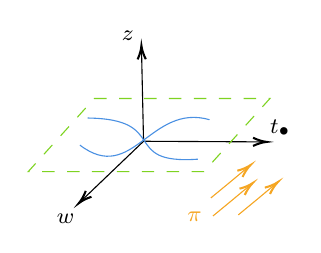
\begin{tikzpicture}[x=0.75pt,y=0.75pt,yscale=-1,xscale=1]
%uncomment if require: \path (0,310); %set diagram left start at 0, and has height of 310

%Straight Lines [id:da8716581873145328] 
\draw    (264,126.5) -- (234.24,154.98) ;
\draw [shift={(232.79,156.36)}, rotate = 316.27] [color={rgb, 255:red, 0; green, 0; blue, 0 }  ][line width=0.75]    (6.56,-1.97) .. controls (4.17,-0.84) and (1.99,-0.18) .. (0,0) .. controls (1.99,0.18) and (4.17,0.84) .. (6.56,1.97)   ;
%Straight Lines [id:da25538335623560116] 
\draw    (264,126.5) -- (263.02,82.45) ;
\draw [shift={(262.97,80.45)}, rotate = 88.72] [color={rgb, 255:red, 0; green, 0; blue, 0 }  ][line width=0.75]    (6.56,-1.97) .. controls (4.17,-0.84) and (1.99,-0.18) .. (0,0) .. controls (1.99,0.18) and (4.17,0.84) .. (6.56,1.97)   ;
%Straight Lines [id:da15856873623352485] 
\draw    (264,126.5) -- (321.32,126.8) ;
\draw [shift={(323.32,126.81)}, rotate = 180.3] [color={rgb, 255:red, 0; green, 0; blue, 0 }  ][line width=0.75]    (6.56,-1.97) .. controls (4.17,-0.84) and (1.99,-0.18) .. (0,0) .. controls (1.99,0.18) and (4.17,0.84) .. (6.56,1.97)   ;
%Curve Lines [id:da31658562114637734] 
\draw [color={rgb, 255:red, 74; green, 144; blue, 226 }  ,draw opacity=1 ]   (237.03,115.3) .. controls (277.26,115.81) and (252.2,137.8) .. (290.2,135.13) ;
%Curve Lines [id:da7192611023303519] 
\draw [color={rgb, 255:red, 74; green, 144; blue, 226 }  ,draw opacity=1 ]   (233.32,128.34) .. controls (258.74,147.7) and (267.21,107.96) .. (295.79,116.11) ;
%Shape: Parallelogram [id:dp48485531317354624] 
\draw  [color={rgb, 255:red, 126; green, 211; blue, 33 }  ,draw opacity=1 ][dash pattern={on 4.5pt off 4.5pt}] (240.24,105.92) -- (324.87,105.92) -- (293.06,141.13) -- (208.44,141.13) -- cycle ;
%Straight Lines [id:da4807100139421694] 
\draw [color={rgb, 255:red, 245; green, 166; blue, 35 }  ,draw opacity=1 ]   (296.42,153.81) -- (305.24,146.55) -- (313.94,139.29) ;
\draw [shift={(315.48,138.01)}, rotate = 140.2] [color={rgb, 255:red, 245; green, 166; blue, 35 }  ,draw opacity=1 ][line width=0.75]    (6.56,-1.97) .. controls (4.17,-0.84) and (1.99,-0.18) .. (0,0) .. controls (1.99,0.18) and (4.17,0.84) .. (6.56,1.97)   ;
%Straight Lines [id:da9540546352598236] 
\draw [color={rgb, 255:red, 245; green, 166; blue, 35 }  ,draw opacity=1 ]   (297.48,162.47) -- (306.29,155.21) -- (315,147.95) ;
\draw [shift={(316.54,146.67)}, rotate = 140.2] [color={rgb, 255:red, 245; green, 166; blue, 35 }  ,draw opacity=1 ][line width=0.75]    (6.56,-1.97) .. controls (4.17,-0.84) and (1.99,-0.18) .. (0,0) .. controls (1.99,0.18) and (4.17,0.84) .. (6.56,1.97)   ;
%Straight Lines [id:da49858931103629067] 
\draw [color={rgb, 255:red, 245; green, 166; blue, 35 }  ,draw opacity=1 ]   (309.66,161.96) -- (318.47,154.7) -- (327.18,147.44) ;
\draw [shift={(328.72,146.16)}, rotate = 140.2] [color={rgb, 255:red, 245; green, 166; blue, 35 }  ,draw opacity=1 ][line width=0.75]    (6.56,-1.97) .. controls (4.17,-0.84) and (1.99,-0.18) .. (0,0) .. controls (1.99,0.18) and (4.17,0.84) .. (6.56,1.97)   ;

% Text Node
\draw (252.28,72.04) node [anchor=north west][inner sep=0.75pt]  [font=\footnotesize] [align=left] {$\displaystyle z$};
% Text Node
\draw (221.02,160.09) node [anchor=north west][inner sep=0.75pt]  [font=\footnotesize] [align=left] {$\displaystyle w$};
% Text Node
\draw (323.76,114.8) node [anchor=north west][inner sep=0.75pt]  [font=\footnotesize] [align=left] {$\displaystyle t_\bullet$};
% Text Node
\draw (283.85,159.17) node [anchor=north west][inner sep=0.75pt]  [font=\footnotesize,color={rgb, 255:red, 245; green, 166; blue, 35 }  ,opacity=1 ] [align=left] {$\displaystyle \pi $};


\end{tikzpicture}
	\caption{}
	\label{fig2}
\end{figure}

By Finite mapping Thm. \ref{lb74}, $\pi_*\scr O_Y$ is a coherent $\scr O_V$-module. By assumption, the Nullstellensatz holds for any coherent ideal $\mc J$ of $\scr O_V$ such that
\begin{align*}
N(\mc J)\subset\{(z,t_\blt)\in V:z=0\}.
\end{align*}
Choose $\mc J=\sann_{\scr O_V}(\pi_*\scr O_Y)$. Then the assumption tells us that there is $n\in\Zbb_+$ such that $z^n\in\scr O_{\Cbb^m,0}$ kills the stalk $(\pi_*\scr O_Y)_0\simeq \scr O_{Y,0}$ (Prop. \ref{lb56}).  So $\pi^\# z^n$ (or simply $z^n$ as an element of $\scr O(\Cbb^{m+1})$) kills $\scr O_{Y,0}=\scr O_{\Cbb^{m+1},0}/\mc I_0$. Therefore $z^n\in\mc I_0$.

Now, in the general case, note that it suffices to prove that $z$ is nilpotent in $z^{<0}\mc I_0=\{f\in\scr O_{\Cbb^{m+1},0}:z^kf\in\mc I_0,k\in\Zbb_+\}$. This statement is true if we can $h\in z^{<0}\mc I_0$ whose series expansion as in \eqref{eq52} has non-zero constant term. This follows by choosing a non-zero $g\in\mc I_0$, letting $k$ be the smallest power of $z$ such that the series expansion of $g$ in $z$ has non-zero coefficient before $z^k$, and setting $h=z^{-k}g$.
\end{proof}



\begin{proof}[\textbf{Proof of Nullstellensatz}]
Let $X$ be a complex space, and assume that $f\in\scr O(X)$ vanishes at every $x\in X$. We now fix $x\in X$ and show that $f$ is nilpotent in $\scr O_{X,x}$. Consider the graph $\fk G(f)$ of $f$, namely the image of the closed embedding $f\vee \id:X\rightarrow \Cbb\times X$ (cf. Prop. \ref{lb80}). Assume $X$ is a small enough neighborhood of $x$ so that $X$ is a closed subspace of an open $U\subset\Cbb^m$ and $x=0_{\Cbb^m}$. Then $\fk G(f)$ is a closed subspace of $\Cbb\times U$. 

As a set, $\fk G(f)$ is contained in $0\times U$. Let $z\in\scr O(\Cbb)$ be the standard coordinate of $\Cbb$. Then by Lemma \ref{lb100}, $z\otimes 1\in\scr O_{\Cbb\times U,0\times 0}$ is nilpotent in $\scr O_{\fk G(f),0\times 0}$. But the restriction $f\vee\id:X\rightarrow\fk G(f)$ is a biholomorphism, and it pulls $z\otimes 1=\pr_\Cbb^\# z$ (where $\pr_\Cbb:\Cbb\times U\rightarrow\Cbb$ is the projection) back to $z\circ \pr_\Cbb\circ(f\vee\id)=z\circ f=f$. So $f$ is nilpotent in $\scr O_{X,0}$.
\end{proof}

\subsection{Examples}


We give an interesting situation to which Nullstellensatz can be applied.


\begin{eg}\label{lb389}
Let $X$ be a complex space and $p\in X$. Let $\varDelta\in\scr O(X)$.  Let $\scr E\subset\scr F$ be a pair of coherent $\scr O_X$-modules. Assume that $\xi\in\scr F(X)$ satisfies that for each $x\in X\setminus N(\varDelta)$, the germ $\xi_x$ belongs to $\scr E_x$. Then $\varDelta_p^k\cdot \xi_p\in\scr E_p$ for some $k\in\Nbb$. 
\end{eg}

\begin{proof}
Let $\scr K=\scr O_X\cdot \xi+\scr E$, which is coherent. Then $\scr E\subset\scr K$, and $\scr E_x=\scr K_x$ when $x\notin N(\Delta)$. Thus $\Supp(\scr K/\scr E)$, as a set, is inside $N(\varDelta)$. So $\varDelta$ vanishes on the set $\Supp(\scr K/\scr E)$. By Rem. \ref{lb115}, there is $k\in\Nbb$ such that $\varDelta_p^k$ kills $\scr K_p/\scr E_p$. So $\varDelta_p^k\cdot\scr K_p\subset\scr E_p$ and hence $\varDelta_p^k\cdot \xi_p\in\scr E_p$. 
\end{proof}

\begin{rem}
The above example is particularly interesting when $X$ is irreducible at $p$ (cf. Def. \ref{lb388}) and $\Delta_p\neq 0$. In that case, the example shows that $\xi_p$ is an $\Kbb$-linear combination of elements of $\scr E_p$, where $\Kbb$ is field of fractions of the integral domain $\scr O_{X,p}$. 

This example suggests why Nullstellensatz is important. Nullstellensatz tells us that in coherent sheaves, all poles are of finite orders. (In Exp. \ref{lb389}, we consider poles at $\varDelta=0$, since $\xi$ belongs to $\scr E$ when restricted to $X\setminus N(\varDelta)$.) In the following, we give another compelling example.  \hfill\qedsymbol
\end{rem}

\begin{eg}
Choose a neighborhood $U$ of $0\in\Cbb$. Choose $f\in\scr O(U\setminus\{0\})$ with infinite poles at $0$, i.e., the Laurant series expansion $f(z)=\sum_{n\in\Zbb}a_nz^n$ satisfies $\inf\{n:a_n\neq0\}=-\infty$. Define an $\scr O_U$-module $\scr E=f\scr O_U+\scr O_U$. More precisely, $\scr E$ is the sheafification of the presheaf associating to each open $V\subset U$ the set of all $f\alpha+\beta|_{V\setminus\{0\}}$ where $\alpha\in\scr O(V\setminus\{0\}),\beta\in\scr O(V)$.

$\scr E$ is clearly of finite type. But $\scr E$ is not coherent:  Otherwise, then $\scr E/\scr O_U$ is coherent. Since $\scr E/\scr O_U$ clearly has support in $\{0\}$, by Nullstellensatz we have $z^k\scr E_0\subset\scr O_{U,0}$. In particular, $(z^kf)_0\in\scr O_{U,0}$. This is impossible.

If, however, $f\in\scr O(U\setminus\{0\})$ has finite poles at $0$, then it is not hard to show that $\scr E$ is coherent: see Prop. \ref{lb187}.
\end{eg}











\begin{subappendices}
\section{Kernels and cokernels in categories of modules}

In a category $\mc C$, if $\varphi,\psi:X\rightarrow Y$ are two morphisms of objects, then the equalizers of double arrow
$\begin{tikzcd}
X \arrow[r,shift left, "\varphi"] \arrow[r,shift right,"\psi"'] & Y
\end{tikzcd}$
can be defined in the same way as in Def. \ref{lb139}. Likewise, a \textbf{coequalizer} \index{00@Coequalizers} of this double arrow is an object $C\in\mc C$ and a morphism $\pi:Y\rightarrow C$ such that $\pi\circ\varphi=\pi\circ\psi$, and that for every object $T$ and morphism $\nu:Y\rightarrow T$ satisfying $\nu\circ\varphi=\nu\circ\psi$ there is a unique morphism $\wtd\nu:C\rightarrow T$ such that $\nu=\wtd\nu\circ\pi$.
\begin{equation}
\begin{tikzcd}
X \arrow[r, "\varphi", shift left] \arrow[r, "\psi"', shift right] & Y \arrow[r, "\pi"] \arrow[rd, "\nu"'] & C \arrow[d, "\wtd\nu", dashed] \\
                                                                   &                                       & T                             
\end{tikzcd}
\end{equation}


Thus, if a functor (resp. contravariant functor) $\fk F:\mc C\rightarrow\mc D$ is an equivalence (resp. antiequivalence) of categories (cf. Thm. \ref{lb19} and \ref{lb49}), then $\fk F$ sends the (co)equalizer of a double arrow $\begin{tikzcd}
X \arrow[r,shift left, "\varphi"] \arrow[r,shift right,"\psi"'] & Y
\end{tikzcd}$
(on the $\mc C$ side) to a (co)equalizer of 
$\begin{tikzcd}
\fk F(X) \arrow[r,shift left, "\fk F(\varphi)"] \arrow[r,shift right,"\fk F(\psi)"'] & \fk F(Y)
\end{tikzcd}$
(resp. sends equalizers to coequalizers of $\begin{tikzcd}
\fk F(Y) \arrow[r,shift left, "\fk F(\varphi)"] \arrow[r,shift right,"\fk F(\psi)"'] & \fk F(X)
\end{tikzcd}$ and coequalizers to equalizers).


The category of modules of a commutative rings and the one of (coherent) $\scr O_X$-modules (where $X$ is a $\Cbb$-ringed space) are both additive categories, which means roughly that one can take direct sums,  that the morphism spaces are abelian groups, and that there is a zero object. A functor between additive functions, called an \textbf{additive functor}, is assumed to preserve the abelian group structures of the morphism spaces. 

Moreover, the above categories are \textbf{abelian categories}. This means that the kernel of a morphism $\varphi:\mc M\rightarrow\mc N$ (which is an object together with the ``inclusion" morphism) is equivalent to the equalizer of $\begin{tikzcd}
\mc M \arrow[r,shift left, "\varphi"] \arrow[r,shift right,"0"'] & \mc N
\end{tikzcd}$
and that the cokernel is equivalent to the coequalizer of this double arrow. From this, it is clear that if a functor (resp. contravariant functor) $\fk F:\mc C\rightarrow\mc D$ is an equivalence (resp. antiequivalence) of abelian categories, then {\color{red}\textit{$\fk F$ must be an exact functor}}, because $\fk F$ commutes with kernels and cokernels (resp. sends kernels to cokernels and cokernels to kernels).



We refer the readers to \cite[Chapter 1]{Vak17} for a more detailed introduction to abelian categories.






\end{subappendices}












\chapter{Local decomposition, singular loci, and dimensions}



\section{Prime decomposition}

We fix a commutative ring $\mc A$. Recall that $\mc A$ is called \textbf{reduced} \index{00@Reduced ring} if $\mc A$ has no non-zero nilpotent elements. This is equivalent to saying that $\{0\}=\sqrt{\{0\}}$. If $I$ is an ideal of $\mc A$, then $\mc A/I$ is reduced iff $\sqrt{I}=I$.

\begin{rem}\label{lb105}
Recall the general fact that for any ideals $I_1,\dots,I_k$ of $\mc A$ we have
\begin{gather}\label{eq53}
\sqrt{I_1\cdots I_k}=\sqrt{I_1\cap\cdots\cap I_k}=\sqrt{I_1}\cap\cdots\cap\sqrt{I_k}.
\end{gather}
In view of Nullstellensatz, the first equality says that ``the zero sets defined by $I_1\cdots I_k$ and defined by $I_1\cap \cdots\cap I_k$ are equal" (namely, they are equal to the union of the zero sets of $I_1,\dots,I_k$). The second equality implies that if $I_i=\sqrt{I_i}$ for each $i$, then $I_1\cap\cdots\cap I_k$ is its own radical.
\end{rem}


\begin{proof}
The two equalities in \eqref{eq53} are clearly $\subset$. If $f\in\cap_i\sqrt I_i$ then $f^{n_i}\in I_i$ for some $n_i\in\Zbb_+$. Then $f^{n_1+\cdots+n_k}\in I_1\cdots I_k$, and hence $f\in\sqrt{I_1\cdots I_k}$. This proves \eqref{eq53}.
\end{proof}

\begin{pp}\label{lb103}
Assume $\mc A$ is reduced. Let $\fk p\subsetneq\mc A$ be an ideal. Then the following are equivalent.
\begin{enumerate}[label=(\alph*)]
\item $\pk$ is a prime ideal.\footnote{Recall that a prime ideal $\pk$ is required not to be the whole ring $\mc A$.} Equivalently, $\mc A/\pk$ is an integral domain.
\item $\pk=\sqrt\pk$. Moreover, if $\pk=I_1\cap I_2$ where $I_1,I_2$ are ideals of $\mc A$, then $I_1=\pk$ or $I_2=\pk$.
\item $\pk=\sqrt\pk$.  Moreover, if $\pk=I_1\cap I_2$ where $I_1,I_2$ are ideals of $\mc A$ satisfying $I_1=\sqrt{I_1}$ and $I_2=\sqrt{I_2}$, then $I_1=\pk$ or $I_2=\pk$.
\end{enumerate}
\end{pp}

We leave it to the readers to figure out the geometric meaning of this lemma (in the case that $\mc A$ is an analytic $\Cbb$-algebra).

\begin{proof}
By replacing $\mc A$ by $\mc A/\pk$, we may assume $\pk=\{0\}$. Clearly (b)$\Rightarrow$(c).

(a)$\Rightarrow$(b): Assume $\{0\}$ is prime. Then clearly $\{0\}=\sqrt{\{0\}}$. Suppose $\{0\}=I_1\cap I_2$ and $I_1,I_2\neq\{0\}$. Then we may choose non-zero $f_i\in I_i$. And $f_1f_2\in I_1\cdot I_2\subset I_1\cap I_2=\{0\}$. So $f_1f_2=0$, contradicting that $\{0\}$ is prime. So (b) follows.

(c)$\Rightarrow$(a). Assume (c). Suppose that there are non-zero $f,g\in \mc A$ such that $fg\in\{0\}$, i.e. $fg=0$. Then as $\mc A$ is reduced, $\{0\}=\sqrt{\{0\}}=\sqrt{f\mc A\cdot g\mc A}=\sqrt{f\mc A}\cap\sqrt{g\mc A}$. This contradicts (c).
\end{proof}


\begin{thm}\label{lb102}
If $\mc A$ is Noetherian and reduced, then there are prime ideals $\fk p_1,\dots,\fk p_N$ of $\mc A$ such that
\begin{align}
\{0\}=\fk p_1\cap\cdots\cap \fk p_N\label{eq55}
\end{align}
and that for each $1\leq i\leq N$,
\begin{align}
\{0\}\neq \bigcap_{j\neq i}\fk p_j.\label{eq56}
\end{align}
Moreover the prime ideals $\pk_1,\dots,\pk_N$ satisfying \eqref{eq55} and \eqref{eq56} are unique. We call this unique decomposition the \textbf{prime decomposition of $\{0\}\subset\mc A$}. \index{00@Prime decomposition}
\end{thm}

The geometric meaning of \eqref{eq55} is that an element $f\in \mc A$ is zero iff $f$ restricts to zero on $\mc A/\pk_i$ (i.e. ``$f$ vanishes on the zero set $N(\pk_i)$") for all $i$.

Note that if $\fk a=\sqrt{\fk a}$ is an ideal of a Noetherian ring $\mc A$, then Thm. \ref{lb102} applied to $\mc A/\fk a$ says that there are prime ideals $\pk_1,\dots,\pk_N$ of $\mc A$ such that
\begin{subequations}\label{eq72}
\begin{gather}
\fk a=\pk_1\cap\cdots\cap\pk_N\\
\fk a\neq \bigcap_{j\neq i}\fk p_j\qquad\forall 1\leq i\leq N
\end{gather}
\end{subequations}
called the \textbf{prime decomposition of $\fk a$}.


\begin{proof}[Proof of the existence]
We first note that if we can find prime ideals $\pk_1,\dots,\pk_N$ satisfying \eqref{eq55}, then by discarding some members of these ideals so that the intersection of the remaining ones is still $\{0\}$ until we cannot do this anymore, \eqref{eq56} is automatically satisfied. So we only need to find prime ideals satisfying \eqref{eq55}.

Let $\fk A$ be the set of all ideals $\fk a$ not equal to $\mc A$ such that $\fk a=\sqrt{\fk a}$ and that $\fk a\subset\mc A$ has no prime decomposition (equivalently, $\fk a$ is not a finite intersection of prime ideals). Note that if $\fk a\in\fk A$, then $\fk a=\sqrt{\fk a}$ and $\fk a$ is not prime. So by Prop. \ref{lb103}, $\fk a=\fk b\cap \fk c$ where the ideals $\fk b,\fk c$ are not $\fk a$ and are the radicals of themselves. One of $\fk b,\fk c$ is not a finite intersection of prime ideals, otherwise $\fk a$ is a finite intersection of prime ideals. So one of $\fk b,\fk c$ is in $\fk A$. 

The above argument shows that if $\fk a_1=\{0\}$ belongs to $\fk A$, then we can construct a strictly increasing infinite chain of elements of $\fk A$: $\fk a_1\subsetneq\fk a_2\subsetneq\fk a_3\subsetneq\cdots$, contradicting that $\mc A$ is Noetherian. So $\{0\}\notin\fk A$.
\end{proof}


\begin{rem}\label{lb106}
In Thm. \ref{lb102}, \eqref{eq55} and \eqref{eq56} imply that
\begin{align*}
\bigcap_{j\neq i}\pk_j\Big\backslash\pk_i\neq\emptyset.
\end{align*}
This means that we can find $f\in \mc A$ which is non-zero when restricted to $\mc A/\pk_i$ (i.e. ``non-zero on $N(\pk_i)$") and zero in the other $\mc A/\pk_j$. Thus, by taking sums, we see that there always exists $f\in \mc A$ which is non-zero precisely when restricted to the given ones of $\mc A/\pk_1,\dots,\mc A/\pk_N$. 
\end{rem}


We remark that when $\mc A$ is not necessarily reduced, there is a generalization called \textbf{primary decomposition}, cf. \cite{AM}. We will not use this notion in out notes.


To prove the uniqueness part of Thm. \ref{lb102} we first need:

\begin{lm}\label{lb107}
In Thm. \ref{lb102}, for each $f\in \mc A$, the annihilator $\Ann_{\mc A}(f)$ equals
\begin{align}\label{eq54}
\Ann_{\mc A}(f)=\bigcap_{
\begin{subarray}{c}
1\leq i\leq N\\[0.2ex]
f\notin\pk_i
\end{subarray}
} \pk_i
\end{align}
\end{lm}

Recall that $\Ann_{\mc A}(f)=\Ann_{\mc A}(f\mc A)$ is the ideal of all $a\in \mc A$ satisfying $af=0$ (Def. \ref{lb104}). Then \eqref{eq54} says that $af=0$ iff $a$ ``vanishes on all $N(\pk_i)$ where $f$ is non-zero on $N(\pk_i)$". See also Prop. \ref{lb178} for a geometric interpretation.





\begin{proof}
Suppose $a\in \mc A$ and $af=0$. Then $af$ restricts to $0$ on the integral domain $\mc A/\pk_i$. If $f\notin \pk_i$ then $f$ is nonzero in $\mc A/\pk_i$. So $a$ is $0$ in $\mc A/\pk_i$. Hence $a\in\pk_i$. Conversely, if $a\in\pk_i$ for all $i$ such that $f\notin\pk_i$, then $af$ belongs to $\pk_i$ for all $1\leq i\leq N$. So $af\in\cap_i\pk_i=\{0\}$.
\end{proof}








Note that when $\mc A$ is reduced, $f$ is a non zero-divisor iff $\Ann_{\mc A}(f)=\{0\}$. Thus:
\begin{co}\label{lb120}
In Thm. \ref{lb102}, $f\in \mc A$ is a non zero-divisor if and only if $f\notin\pk_i$ for all $1\leq i\leq N$.
\end{co}






Now the uniqueness of prime decomposition follows immediately from the following fact:

\begin{pp}\label{lb291}
In Thm. \ref{lb102}, $\pk_1,\dots,\pk_N$ are precisely the \textbf{associated primes} \index{00@Associated primes} of $\mc A$, i.e. prime ideals of the form $\Ann_{\mc A}(f)$ for some $f\in \mc A$.
\end{pp}


\begin{proof}
We first note that an intersection of more than one members of $\pk_1,\dots,\pk_N$ is not prime. This together with Lemma \ref{lb107} would imply that $\Ann_{\mc A}(f)$ is prime only if $\Ann_{\mc A}(f)=\pk_i$ for some $i$, and hence that the associated primes are among $\pk_1,\dots,\pk_N$. To prove the claim, consider for instance $\pk=\pk_1\cap\pk_2\cap\cdots\cap\pk_k$ where $k>1$. Suppose $\pk$ is prime. Then by Prop. \ref{lb103}, either $\pk_1$ or $\pk_2\cap\cdots\cap\pk_k$ equals $\pk$, contradicting \eqref{eq56}. So $\pk$ cannot be prime.

For each $i$, by Rem. \ref{lb106} we can choose $f\in \mc A$ non-zero on $\mc A/\pk_i$ but zero on $\mc A/\pk_j$ whenever $j\neq i$. Then $\pk_i=\Ann_{\mc A}(f)$ by Lemma \ref{lb107}, which shows that $\pk_i$ must be an associated prime.
\end{proof}


We now give another characterization of the prime components of a reduced Noetherian ring.

\begin{lm}\label{lb376}
Let $\mc A$ be Noetherian and reduced with prime decomposition $\{0\}=\pk_1\cap\cdots\cap\pk_N$. Let $\pk\subset\mc A$ be a prime ideal. Then $\pk_i\subset\pk$ for some $1\leq i\leq N$.
\end{lm}

\begin{proof}
Suppose that for each $i$ we have $\pk_i\nsubset\pk$. Then there exists $f_i\in\pk_i\setminus\pk$. The primeness of $\pk$ implies that  $f=f_1\cdots f_N$ is not in $\pk$. But $f$ is in $\pk_1\cap\cdots\cap \pk_N=\{0\}$. So $0\notin\pk$, impossible.
\end{proof}


\begin{pp}\label{lb374}
Let $\mc A$ be Noetherian and reduced with prime decomposition $\{0\}=\pk_1\cap\cdots\cap\pk_N$. Let $\pk\subset\mc A$ be a prime ideal. The following are equivalent.
\begin{enumerate}[label=(\arabic*)]
\item $\pk=\pk_i$ for some $1\leq i\leq N$.
\item $\pk$ is a minimal prime ideal of $\mc A$. Namely, if $\fk q$ is a prime ideal of $\mc A$ and if $\fk q\subset\pk$, then $\fk q=\pk$.
\end{enumerate}
\end{pp}

\begin{proof}
(1)$\Rightarrow$(2): Let us prove for instance that $\pk_1$ is minimal. Suppose $\fk q\subset\pk_1$ is a prime ideal of $\mc A$, then $\{0\}=\fk q\cap\pk_2\cap\cdots\cap\pk_N$. Then some members of $\fk q,\pk_2,\dots,\pk_N$ give the prime decomposition of $\{0\}\subset\mc A$. By the uniqueness of prime decomposition, the number of these members must be $N$, and $\fk q=\pk_1$.

(2)$\Rightarrow$(1): By Lem. \ref{lb376}.
\end{proof}










\section{Reduction $\red(X)$ and coherence of $\sqrt{\mc I}$}\label{lb381}


In this section we study the reduction of complex spaces. The main results Thm. \ref{lb108} and equivalently Thm. \ref{lb109} are originally due to Oka and H. Cartan. Some key ingredients of the proof are prime decomposition, Nullstellensatz, and the ranks of Jacobian matrices (which are a guise for embedding dimensions to be studied later). Our approach follows \cite{GPR}.

\subsection{Main results and consequences}

\begin{thm}\label{lb108}
Let $X$ be a complex space reduced at a point $x$. There $X$ is reduced on a neighborhood $U$ of $x$.
\end{thm}



This theorem is equivalent to:

\begin{thm}\label{lb109}
Let $X$ be a complex space. Then for each coherent ideal $\mc I$ of $\scr O_X$, its radical $\sqrt{\mc I}$ is coherent.
\end{thm}


\begin{rem}
Note that Thm. \ref{lb109} is equivalent to the seemingly special case that for each complex space $X$, $\sqrt{0_X}$ is coherent. Indeed, if this special case is true, let $Y=\Specan(\scr O_X/\mc I)$. Then $\sqrt{0_Y}$ is (or more precisely, $\iota_{Y,X,*}\sqrt{0_Y}$ is)
\begin{align}
\sqrt{0_Y}=\sqrt{\mc I/\mc I}=\sqrt{\mc I}/\mc I.
\end{align}
So $\sqrt{\mc I}/\mc I$ is coherent, and hence $\sqrt{\mc I}$ is coherent. Therefore Thm. \ref{lb109} holds.
\end{rem}


\begin{proof}[Proof that Thm. \ref{lb108} and \ref{lb109} are equivalent]
Assume Thm. \ref{lb109}. Assume $X$ is reduced at $x$. Then $\sqrt{\mc I}$ is coherent and its stalk at $x$ is $0$. So its stalks are zero everywhere on a neighborhood $U$ of $x$. Then $X$ is reduced everywhere on $U$.

Assume Thm. \ref{lb108}. Choose any complex space $X$ and coherent ideal $\mc I$. Choose $x\in X$. Since $\scr O_{X,x}$ is Noetherian, $\sqrt{\mc I}_x$ is generated by finitely many elements $f_1,f_2,\dots$. By shrinking $X$ to a neighborhood of $x$, we assume $f_1,f_2,\dots\in\sqrt{\mc I}(X)$. Let $\mc J$ be the ideal generated by $f_1,f_2,\dots$. Then $\mc J\subset\sqrt{\mc I}$ and $\mc J_x=\sqrt{\mc I}_x$. This implies that  $Y=\Specan(\scr O_X/\mc J)$ is reduced at $x$ (since $\sqrt{0_{Y,x}}=\sqrt{\mc J_x}/\mc J_x$). 

$\mc J_x=\sqrt{\mc I}_x$ also implies $\mc I_x\subset\mc J_x$. Therefore, since $\mc I$ is coherent, by Rem. \ref{lb17} we may shrink $X$ so that $\mc I\subset\mc J$. We conclude that
\begin{align*}
\mc I\subset\mc J\subset\sqrt{\mc I}\subset \sqrt{\mc J}.
\end{align*}
By Thm. \ref{lb108}, we may shrink $X$ so that $Y$ is reduced everywhere on $X$. This means $\mc J=\sqrt{\mc J}$, which proves that $\sqrt{\mc I}$ equals $\mc J$ and is therefore coherent.
\end{proof}

\begin{co}
Let $X$ be a complex space. Then for each analytic subset $A$ of $X$, the \textbf{ideal associated to $A$} defined by \index{00@Ideal $\scr I_A$ associated to an analytic subset} \index{IA@$\scr I_A$}
\begin{align}
\scr I_A(U)=\{f\in\scr O_X(U):f(x)=0\quad\forall x\in A\cap U\} \label{eq67}
\end{align}
(for all open $U\subset X$) is coherent.
\end{co}




\begin{proof}
If $A=N(\mc I)$ for some coherent ideal $\mc I$ then
\begin{align}
\scr I_A=\sqrt{\mc I}.
\end{align}
\end{proof}

\begin{rem}\label{lb118}
Let $X$ be a reduced complex space. By Nullstellensatz, we have a bijection
\begin{gather}
\begin{gathered}
\{\text{Analytic subsets of $X$}\}\xleftrightarrow{\simeq} \{\text{Coherent ideals  $\mc I\subset\scr O_X$ satisfying }\mc I=\sqrt{\mc I}\}\\
A\mapsto \scr I_A\qquad N(\mc I)\mapsfrom \mc I
\end{gathered}
\end{gather}
If $A,B$ are analytic subsets of $X$ then clearly
\begin{align*}
A\subset B\quad \Longleftrightarrow \quad \scr I_A\supset\scr I_B
\end{align*}
$A\cap B$ and $A\cup B$ are both analytic subsets of $X$, and we indeed have
\begin{gather}
\scr I_{A\cap B}=\sqrt{\scr I_A+\scr I_B}\qquad \scr I_{A\cup B}=\scr I_A\cap\scr I_B=\sqrt{\scr I_A\cdot\scr I_B}
\end{gather}
\end{rem}

\begin{proof}
It is clear that the coherent ideals (cf. Cor. \ref{lb110} for the coherence) $\scr I_A+\scr I_B$ has zero set $A\cap B$ and $\scr I_A\cdot\scr I_B$ has zero set $A\cup B$.  And $\sqrt{\scr I_A\cdot\scr I_B}=\scr I_A\cap\scr I_B$ by Rem. \ref{lb105}.
\end{proof}



\begin{rem}\label{lb127}
We often identify an analytic subset $A$ with the corresponding reduced complex subspace $\Specan(\scr O_X/\scr I_A)$. \index{00@Analytic subsets(=reduced complex subspaces)} In that case ``analytic subsets" and ``reduced complex subspaces" are synonymous. But there is one exception. The intersection of analytic subsets $A\cap B$ is usually not the intersection of two (reduced) complex spaces (as defined in Exp. \ref{lb79}): In the former case $A\cap B$ is determined by the ideal $\scr I_{A\cap B}=\sqrt{\scr I_A+\scr I_B}$ and the latter case $\scr I_A+\scr I_B$. {\color{red}\textit{So we will make distinctions between analytic subsets and reduced complex subspaces when taking intersections.}} 

There is no such a problem when taking unions: We haven't defined unions for closed complex subspaces, since both $\mc I_1\cap \mc I_2$ and $\mc I_1\cdot\mc I_2$ are reasonable ideals for defining the union. Certainly, for analytic subspaces, $\scr I_{A\cap B}$ is the correct ideal defining the union.   \hfill\qedsymbol
\end{rem}



\begin{co}\label{lb135}
Let $X$ be a complex space. Then the set of all non-reduced points of $X$ is an analytic subset of $X$.
\end{co}


\begin{proof}
$x\in X$ is not reduced iff $x\in\Supp(\sqrt{0_X})$.
\end{proof}



\begin{co}\label{lb136}
Let $A$ be a subset of a complex space $X$. Then the following are equivalent:
\begin{enumerate}[label=(\arabic*)]
\item $A$ is an analytic subset of $X$. (Recall this means that $A=N(\mc I)$ for a coherent ideal $\mc I\subset\scr O_X$.)
\item Each $x\in X$ is contained in a neighborhood $U$ such that $A\cap U$ is analytic in $U$.
\end{enumerate}
\end{co}


Therefore $A$ is analytic iff each $x\in X$ is contained in a neighborhood $U$ such that $A\cap U$ is the zero set of finitely many elements of $\scr O(U)$.


\begin{proof}
Clearly (1)$\Rightarrow$(2). Assume (2). Let $\scr I_A$ be defined by \eqref{eq67}. For each $x\in X$ there is a neighborhood $U$ of $x$ such that $A\cap U$ is analytic, i.e. $A\cap U=N(\mc I_U)$ for a coherent ideal $\mc I_U$ of $\scr O_U$. Then $\scr I_A|_U$ equals $\scr I_{A\cap U}=\sqrt{\mc I_U}$ which is coherent. Therefore $\scr I_A$ is coherent. We have $N(\scr I_A)=A$ since $N(\scr I_A)\cap U=N(\scr I_{A\cap U})=A\cap U$. So $A$ is analytic.
\end{proof}








\begin{df}\label{lb390}
Let $X$ be a complex space. Then the reduced space \index{00@Reduction $\red(X)$ of a complex space $X$}
\begin{align*}
\red(X)=\Specan(\scr O_X/\sqrt{0_X})
\end{align*}
is called the \textbf{reduction} of $X$.
\end{df}







\subsection{Proof of Thm. \ref{lb108}}

\begin{df}\label{lb388}
We say that a complex space $X$ is \textbf{irreducible at $x$} \index{00@Irreducible at a point} if $\scr O_{X,x}$ is an integral domain. (Note that if $X$ is irreducible at $x$ then $X$ is reduced at $x$.) We say that $X$ is \textbf{locally irreducible} \index{00@Locally irreducible} if $X$ is irreducible at every point of $X$.  If $X$ is not irreducible at $x$, we say that $X$ is \textbf{reducible at $x$}. \index{00@Reducible at a point} (Note that ``reducible"$\neq$``reduced"!)
\end{df}



\begin{lm}\label{lb117}
Suppose that Thm. \ref{lb108} holds whenever $X$ is irreducible at $x$. Then Thm. \ref{lb108} holds in general.
\end{lm}


\begin{proof}
Assume $\scr O_{X,x}$ is reduced. Apply prime decomposition (Thm. \ref{lb102}) to $A=\scr O_{X,x}$ to get $\{0\}=\pk_1\cap\cdots\cap\pk_N$. By shrinking $X$ to a neighborhood of $x$ we assume each $\pk_i$ is the stalk $\scr P_{i,x}$ of a coherent ideal $\scr P_i$ of $\scr O_X$. Let $Y_i=\Specan(\scr O_X/\scr P_i)$. Then $Y_i$ is irreducible at $x$. Since $\bigcap_{i=1}^N\scr P_i$ is $\scr O_X$-coherent (Cor. \ref{lb110}), we may shrink $X$ so that $\bigcap_i \scr P_{i,y}=\{0\}$ for all $y\in X$.

By assumption, we can shrink $X$ further so that each $Y_i$ is reduced everywhere. This means that for each $y\in X$ we have $\scr P_{i,y}=\sqrt{\scr P_{i,y}}$. Therefore by Rem. \ref{lb105}, the zero ideal of $\scr O_{X,y}$ is its own radical. So $\scr O_{X,y}$ is reduced.
\end{proof}







\begin{lm}\label{lb112}
Let $X$ be a model space irreducible at $0\in X$. Then after shrinking $X$ to a neighborhood of $0$, there exists $\varDelta\in\scr O(X)$ whose germ at $0$ is non-zero such that $X$ is smooth outside $N(\varDelta)$. 
\end{lm}








\begin{proof}[\textbf{Proof of Thm. \ref{lb108}}]
By Lemma \ref{lb117}, it suffices to assume that $X$ is a complex model space irreducible (and hence reduced) at $0$.  Assume that the statement in Lemma \ref{lb112} holds. Since $\varDelta$ is non-zero in the integral domain $\scr O_{X,0}$, $\varDelta$ is a non zero-divisor of $\scr O_{X,0}$. Therefore, by Prop. \ref{lb113}, we may shrink $X$ to a neighborhood of $0$ so that $\varDelta$ is a non zero-divisor of $\scr O_{X,x}$ for all $x\in X$.

Choose any open $V\subset X$ and $f\in\sqrt{0_X}(V)$. Since $X\setminus N(\varDelta)$ is a complex manifold, $\sqrt{0_{X\setminus N(\varDelta)}}=0$. So the support of $f$, or more precisely $\Supp(f\scr O_V)$, is inside $N(\varDelta)$. So $\varDelta$ vanishes on $\Supp(f\scr O_V)$. Therefore, by Nullstellensatz (Rem. \ref{lb115}-3), for each $x\in V$ there is $n\in\Nbb$ such that $f\varDelta^n=0$ in $\scr O_{X,x}$. This proves $f=0$ in $\scr O_{X,x}$ because $\varDelta$ is a non zero-divisor. Therefore $\sqrt{0_X}=0$.
\end{proof}







We shall give two proofs of Lemma \ref{lb112}. The first one is given in Sec. \ref{lb119} which relies on the following preliminary Lemma. The second proof is given in Subsec. \ref{lb380}.



\begin{lm}\label{lb111}
Let $(w_1,\dots,w_m,z_1,\dots,z_n)$ be the standard coordinates of $\Cbb^{m+n}$. Let $I$ be an ideal of $\scr A=\scr O_{\Cbb^{m+n},0}$ such that $I\neq\scr A$. Suppose that $\partial_{z_1}I\subset I,\dots,\partial_{z_n}I\subset I$. Then $I\subset w_1\scr A+\cdots+w_m\scr A$.
\end{lm}


\begin{proof}
Note that $I\neq\scr A$ means that all elements of $I$ vanish at $0$. Now $\partial_{z_\blt}I\subset I$ implies that all higher partial derivatives over $z_1,\dots,z_n$ of $f\in I$ are in $I$, and hence vanish at $0$. Therefore the restriction of $f$ to $0_{\Cbb^m}\times\Cbb^n$ must be constantly zero, since its power series expansion at $0$ is zero. But the ideal of elements of $\scr A$ vanishing on $0\times\Cbb^n$ is precisely $w_1\scr A+\cdots+w_m\scr A$. This finishes the proof.
\end{proof}



\section{Local decomposition of reduced complex spaces}


\subsection{Germs of analytic subsets and ideals}\label{lb157}


Fix a complex space $X$. Suppose that $X$ is reduced and $x\in X$. Then similar to Rem. \ref{lb118}, we have a bijection $A\mapsto I_A,N(I)\mapsfrom I$:
\begin{enumerate}[label=(\arabic*)]
\item Germs of analytic subsets of $X$ at $x$.
\item Ideals $I\subset\scr O_{X,x}$ satisfying $I=\sqrt I$.
\end{enumerate}
Indeed, (1) are precisely the germs of closed reduced complex subspaces of $X$ passing through $x$, and (2) are precisely the germs of coherent ideals $\mc I\subset\scr O_X$ at $x$ satisfying $\mc I=\sqrt{\mc I}$ (cf. Thm. \ref{lb49}). 

\begin{rem}
To be more explicit, if a germ $A$ in (1) is represented by an analytic subset $A$ closed in a neighborhood $U$ of $x$, then the stalk at $x$ of $\scr I_A=\{f\in\scr O_U:f(y)=0,\forall y\in A\}$ gives the corresponding ideal $I_A$ in (2). Conversely, given an ideal $I$ in (2) which is finitely generated because $\scr O_{X,x}$ is Noetherian, let $f_1,\dots,f_k\in I$ generate $I$, and choose a neighborhood $U\subset X$ of $x$ such that $f_1,\dots,f_k\in\scr O_X(U)$. Then the germ at $x$ of $N(f_1\scr O_U+\cdots+f_k\scr O_U)$ gives the germ $N(I)$ in (1).
\end{rem}




\begin{rem}\label{lb128}
We list some easy but useful facts about this correspondence. Let $(X,x)$ be a germ of reduced complex space.
\begin{itemize}
\item $I_{A\cup B}=I_A\cap I_B=\sqrt{I_A\cdot I_B}$.
\item By Prop. \ref{lb103}-(c), $\scr O_{X,x}$ is an integral domain if and only if $(X,x)$ is an irreducible germ, namely if $(X,x)=(A,x)\cup (B,x)$ where $(A,x),(B,x)$ are germs of analytic subsets then $(A,x)=(X,x)$ or $(B,x)=(X,x)$.
\begin{itemize}
\item More precisely, $\scr O_{X,x}$ is an integral domain iff for every neighborhood $U$ of $x$ written as $U=A\cup B$ where $A,B$ are analytic subsets of $U$, one of $A$ and $B$ contains a neighborhood of $x\in X$.
\end{itemize}
\end{itemize}
\end{rem}

\subsection{Local decomposition}


\begin{thm}\label{lb124}
Let $X$ be a reduced complex space and $x\in X$. Then after shrinking $X$ to a neighborhood of $x$, we have
\begin{align}
X=X_1\cup\cdots\cup X_N  \label{eq61}
\end{align}
where each $X_i$ is an analytic subset of $X$ which is irreducible at $x$, and for each $1\leq i\leq N$,
\begin{align}
\bigcup_{j\neq i}X_j\quad\textnormal{contains no neighborhoods of }x\in X.\label{eq62}
\end{align}
Such decomposition of $X$ is unique up to shrinking $X$ to smaller neighborhoods of $x$. We call it the \textbf{local decomposition} (or \textbf{irreducible decomposition}) of $X$ at $x$. \index{00@Local/irreducible decomposition of $X$ at $x$} Moreover, we have
\begin{align}
\{0\}=\scr I_{X_1,x}\cap\cdots\cap\scr I_{X_N,x}  \label{eq63}
\end{align}
which gives the prime decomposition of $\{0\}\subset\scr O_{X,x}$.
\end{thm}

Note that (assuming \eqref{eq61} then) \eqref{eq62} is equivalent to saying that
\begin{align}\label{eq64}
X\Big\backslash \bigcup_{j\neq i}X_j=X_i\Big\backslash \bigcup_{j\neq i}X_j\quad\text{intersects every neighborhood of }x\in X.
\end{align}


\begin{proof}
Uniqueness: Every local decomposition \eqref{eq61} clearly gives a prime decomposition \eqref{eq63}, where the condition $\bigcap_{j\neq i}\scr I_{X_j,x}\neq 0$ corresponds precisely to \eqref{eq62}. The uniqueness of prime decomposition implies the uniqueness of local decomposition.

Existence: Let $\{0\}=\pk_1\cap\cdots\cap\pk_N$ be the prime decomposition of $\{0\}\subset\scr O_{X,x}$. By shrinking $X$, for each $i$ we may find a coherent ideal $\scr P_i$ whose stalk at $x$ is $\pk_i$. Since $\scr P_1\cap\cdots\cap\scr P_N$ is coherent (Cor. \ref{lb110}), we can shrink $X$ further so that $\scr P_1\cap\cdots\cap\scr P_N=0_X$. So by Rem. \ref{lb105},
\begin{align*}
X=N(0_X)=N(\scr P_1\cap\cdots\cap\scr P_N)=N(\scr P_1\cdots\scr P_N)=X_1\cup\cdots\cup X_N.
\end{align*}
This gives a local decomposition.
\end{proof}


Lem. \ref{lb107} has the following geometric interpretation:

\begin{pp}\label{lb378}
Let $X$ be a reduced complex space and $f\in\scr O(X)$. Then $\Supp(f\scr O_X)$ (cf. Def. \ref{lb186}) is reduced. Suppose that $X$ has local decomposition $X=X_1\cup\cdots\cup X_N$ at $x$. Then 
\begin{align}\label{eq193}
\big(\Supp(f\scr O_X),x\big)=\bigcup_{
\begin{subarray}{c}
1\leq i\leq N\\[0.3ex]
f_x\notin\scr I_{X_i,x}
\end{subarray}
} (X_i,x)
\end{align}
\end{pp}

\begin{proof}
The germ of the complex space $\Supp(f\scr O_X)$ at $x$ is $\scr O_{X/x}/\Ann_{\scr O_{X,x}}(f)$. By Lem. \ref{lb107}, the ideal $\Ann_{\scr O_{X,x}}(f)$ is its own radical (cf. \eqref{eq53}), and the germ of zero set of $\Ann_{\scr O_{X,x}}(f)$ equals the RHS of \eqref{eq193} by Rem. \ref{lb128}.
\end{proof}




Property \eqref{eq62} can be upgraded to the following form:

\begin{thm}\label{lb125}
Let $X=X_1\cup\cdots\cup X_N$ be a local decomposition of a reduced complex space $X$ at $x$. Then after shrinking $X$ to a neighborhood of $x$, for each $i\neq j$,
\begin{align}
X_i\cap X_j~~\text{is nowhere dense in }X_i\label{eq65}
\end{align}
In that case, $X$ is reducible at each point of $X_i\cap X_j$ where $i\neq j$.
\end{thm}

Note that \eqref{eq65} implies, for instance, that if $1\leq k<N$ then $(X_1\cup\cdots\cup X_k)\cap (X_{k+1}\cup\cdots\cup X_N)$ is nowhere dense in every $X_i$. Hence it is nowhere dense in any union of subclass of $X_1,\dots,X_N$.


We will prove Thm. \ref{lb125} in Sec. \ref{lb126}. Note that (cf. Rem. \ref{lb127}) here $X_i\cap X_j$ means set-theoretic intersection (i.e. intersection of analytic subsets), not intersection of complex spaces. But this is not really a big issue here; we are just reminding the readers of the conventions we set before.


It is easy to see that if $X_1,\dots,X_N$ are irreducible at $x$ and if \eqref{eq65} is satisfied for all $i\neq j$, then \eqref{eq62} is satisfied, and hence $X=X_1\cup\cdots\cup X_N$ is the unique local decomposition of $X$ at $x$. This observation can be generalized:

\begin{pp}\label{lb214}
Let $X=X_1\cup\cdots\cup X_N$ be a decomposition of reduced complex space $X$ into analytic subsets. Choose $x\in X_1\cap\cdots\cap X_N$. Assume $X$ is small enough such that for each $1\leq i\leq N$, $X_i$ has a local decomposition
\begin{align*}
X_i=X_{i,1}\cup X_{i,2}\cup\cdots
\end{align*}
at $x$. Assume that \eqref{eq65} holds for all $1\leq i\neq j\leq N$. Then
\begin{align*}
X=\bigcup_{i,k}X_{i,k}
\end{align*}
is the local decomposition of $X$ at $x$.
\end{pp}

\begin{proof}
It suffices to show that, after shrinking $X$ to a neighborhood of $x$, $X_{i,k}\cap X_{j,l}$ is nowhere dense in $X_{i,k}$ if $(i,k)\neq (j,l)$. By Thm. \ref{lb125}, we may shrink $X$ so that this is true whenever $i=j$. So let us assume $i\neq j$. Suppose that $X_{i,k}\cap X_{j,l}$ contains a non-empty open subset $U$ of $X_{i,k}$.  Let $A=\bigcup_{k'\neq k}X_{i,k'}$. Then $U\setminus A$ is an open subset of $X_{i,k}\setminus A=X_i\setminus A$ and hence is open in $X_i$. $U\setminus A$ is nonempty because $X_{i,k}\cap A$ is nowhere dense in $X_{i,k}$. So $U\setminus A$ is a nonempty subset of $X_i\cap X_j$ and is open in $X_i$, impossible.
\end{proof}









\section{Non zero-divisors and nowhere dense analytic subsets}\label{lb126}


As an application of local decomposition, we give an extremely useful geometric characterization of non-zero divisors:





\begin{pp}\label{lb121}
Let $X$ be a reduced complex space and $x\in X$. Choose $f\in\scr O(X)$. Then the following are equivalent. 
\begin{enumerate}[label=(\arabic*)]
\item $f$ is a non zero-divisor of $\scr O_{X,x}$.
\item There is a neighborhood $U\subset X$ of $x$ such that $N(f)\cap U$ is nowhere dense in $U$.
\end{enumerate}
\end{pp}

\begin{proof}
Assume (1) is true. Then by Prop. \ref{lb113}, after shrinking $X$ to a neighborhood of $x$, $f$ is a non-zero divisor of $\scr O_{X,p}$ for all $p\in X$. If $N(f)$ contains an open subset $V$ of $X$, then $f$ takes value zero everywhere on $V$. So $f|_V=0$ because $X$ is reduced, contradicting the fact that $f$ is a non zero-divisor of $\scr O_{V,p}$ when $p\in V$.  So (2) must be true.

Assume that (1) is not true. By shrinking $X$, we may find a local decomposition $X=X_1\cup\cdots\cup X_N$ at $x$. By Cor. \ref{lb120}, the germ of $f$ at $x$ belongs to $\scr I_{X_i,x}$ for some $i$. Shrink $X$ so that $f\in\scr I_{X_i}(X)$. Then $f$ vanishes on $X_i$. Thus, by \eqref{eq64}, $N(f)\supset X_i$ contains the non-empty open subset $X\setminus \bigcup_{j\neq i}X_j$ of $X$. So (2) is not true.
\end{proof}

Thus, we get a function-theoretic characterization of irreducible points. One may compare this characterization with its global version Thm. \ref{lb240}.

\begin{co}\label{lb369}
Let $X$ be a reduced complex space and $x\in X$. The following are equivalent:
\begin{enumerate}[label=(\arabic*)]
\item $X$ is irreducible at $x$.
\item For every nonzero $f\in\scr O_{X,x}$ there is a neighborhood $U\subset X$ of $x$ such that $N(f)\cap U$ is nowhere dense in $U$.
\end{enumerate}
\end{co}





The following can be compared with Cor. \ref{lb239}.

\begin{co}\label{lb177}
Let $X$ be a reduced complex space and $x\in X$. The following are equivalent:
\begin{enumerate}[label=(\arabic*)]
\item $X$ is irreducible at $x$.
\item For every germ of analytic subset $(A,x)$, either $(A,x)=(X,x)$, or there is a neighborhood $U$ of $x\in X$ such that $A\cap U$ is nowhere dense  of $U$. 
\end{enumerate}
\end{co}

\begin{proof}
Assume (1). For each $(A,x)\subsetneq(X,x)$, since $\scr J_{A,x}\neq 0$, we choose a nonzero $f\in\scr J_{A,x}$. By Cor. \ref{lb369}, there is a neighborhood $U$ of $x\in X$ such that $N(f)\cap U$ (which contains $A\cap U$) is nowhere dense analytic in $U$. This proves (2).

Assume (2). Then for every nonzero $f\in\scr O_{X,x}$, since $(N(f),x)\subsetneq(X,x)$, there is a neighborhood $U$ of $x$ such that $N(f)\cap U$ is nowhere dense in $U$. So (1) follows from Cor. \ref{lb369}.
\end{proof}

We are now ready to prove Thm. \ref{lb125}.



\begin{proof}[\textbf{Proof of Thm. \ref{lb125}}]
We set $A=X_i,B=X_j$ for simplicity. Since their germs satisfy $(A,x)\nsubset(B,x)$, we have $(A\cap B,x)\subsetneq (A,x)$. So, by Cor. \ref{lb177}, after shrinking $X$ to a neighborhood of $x$, $A\cap B$ is nowhere dense in $A$. This proves \eqref{eq65}.

Now assume that \eqref{eq65} holds for all $i\neq j$. Let $y\in A\cap B$. Since $A\cap B$ is nowhere dense in $B$, we have  $(A,y)\subsetneq (A\cup B,y)$. Similarly, since $A\cap B$ is nowhere dense in $A$, we have  $(B,y)\subsetneq (A\cup B,y)$. This proves the last sentence of Thm. \ref{lb125}, thanks to Rem. \ref{lb128}.
\end{proof}






\begin{rem}\label{lb122}
Prop. \ref{lb121} can be used in the following way. 
\begin{itemize}
\item Suppose $A$ is an analytic subset of a reduced space $X$. To show that $A$ is nowhere dense, it suffices to prove that for each $x\in A$ there is a non zero-divisor $f\in\scr O_{X,x}$ vanishing on $A\cap U$ for a neighborhood $U$ of $x$. Then after shrinking $U$, $N(f)\cap U$ is nowhere dense. So its subset $A\cap U$ is nowhere dense.
\end{itemize}
Actually, if $A$ is expected to be nowhere dense, then one must be able to find such $f$ due to the following generalization of Prop. \ref{lb121} (which can be viewed as the complex-analytic version of prime avoidance lemma, cf. \cite[Sec. 11.2]{Vak17} or \cite[Sec. 3.2]{Eis}):
\end{rem}



\begin{pp}\label{lb123}
Let $X$ be a reduced complex space and $\mc I$ a coherent ideal of $\scr O_X$. Let $A=N(\mc I)$. The following are equivalent.
\begin{enumerate}[label=(\arabic*)]
\item $A$ is nowhere dense in $X$.
\item For each $x\in X$, $\mc I_x$ contains a non zero-divisor of $\scr O_{X,x}$.
\end{enumerate}
\end{pp}

Another description of nowhere dense analytic subsets is given by Ritt's lemma \ref{lb147}.


\begin{proof}
(2)$\Rightarrow$(1) is already explained in Rem. \ref{lb122}. Let us prove (1)$\Rightarrow$(2).

Assume that $A$ is nowhere dense. By shrinking $X$ to a neighborhood of $x$ we may find a local decomposition $X=X_1\cup\cdots\cup X_N$ at $x$.  For each $i$, we have $(X_i,x)\nsubset(A,x)$, namely, we cannot find any neighborhood $U\subset X$ of $x$ such that $X_i\cap U\subset A\cap U$: Otherwise, by \eqref{eq64}, $X_i$ contains an open subset (namely $X_i\setminus\bigcap_{j\neq i} X_j$) which intersects $U$, contradicting the fact that $A$ is nowhere dense. 

Therefore, we have $\scr I_{A,x}\nsubset \scr I_{X_i,x}$ for all $i$. Since $\sqrt{\mc I_x}=\scr I_{A,x}$ and $\scr I_{X_i,x}$ is its own radical, we have $\mc I_x\nsubset\scr I_{X_i,x}$. The existence of a non zero-divisor follows from the next lemma.
\end{proof}






\begin{lm}\label{lb145}
Let $X=X^1\cup\cdots\cup X^N$ be a decomposition of reduced complex space $X$ into analytic subsets. Let $x\in X$, and assume that each $X^j$ has a local decomposition at $x$:
\begin{align*}
X^j=X^j_1\cup X^j_2\cup\cdots
\end{align*}
Suppose that we have a linear subspace $\scr W\subset\scr O_{X,x}$ such that
\begin{align*}
\scr W\nsubset \scr I_{X^j_i,x}\qquad (\forall i,j)
\end{align*}
Then there is an element of $\scr W$ which is a non zero-divisor of $\scr O_{X^1,x},\dots,\scr O_{X^N,x}$.
\end{lm}

\begin{proof}
Since each $\scr W\cap \scr I_{X^j_i,x}$ is not the full space $\scr W$, the \textit{finite} union $\bigcup_{i,j} (\scr W\cap\scr I_{X_i^j,x})=\scr W\cap \big(\bigcup_{i,j}\scr I_{X_i^j,x}\big)$ is not $\scr W$. So there is an element $f\in\scr W$ which is not in $\bigcup_{i,j}\scr I_{X_i^j,x}$. By Cor. \ref{lb120}, $f$ is a non zero-divisor of each $\scr O_{X^j,x}$.
\end{proof}

Note that in the above proof we have used the fact that $\Cbb$ is an infinite field. Over a finite field, a finite union of proper linear subspaces might be the full linear space.

























\section{Ranks of Jacobian matrices and singular loci}\label{lb119}



This section can be read immediately after Sec. \ref{lb381}. The goal of this section is to prove Lemma \ref{lb112}, a crucial ingredient in the proof that any complex space reduced at a point is reduced near that point (Thm. \ref{lb108}). Indeed, even if we assume that a complex space is reduced everywhere, this lemma still tells us something interesting: it says that if $X$ is irreducible at $0$ then, after shrinking $X$ to a neighborhood of $0$, $X$ is smooth outside a nowhere dense analytic subset (due to Prop. \ref{lb121}). 

The proof of Lemma \ref{lb112} relies on Jacobian matrices, which are very useful for determining the singular locus of a complex space.


\begin{df}
If $X$ is a complex space, we define the \textbf{singular locus} of $X$ \index{00@Singular locus $\Sg(X)$} to be the closed (cf. Cor. \ref{lb130}) subset 
\begin{align*}
\Sg(X)=\{x\in X:X\text{ is not smooth at }x\}.
\end{align*}
\end{df}



\subsection{Jacobian matrices}\label{lb116}




Assume $X=\Specan(\scr O_U/\mc I)$ is a closed subspace of an open $U\subset\Cbb^m$, where $\mc I$ is generated by $f^1,\dots,f^n\in\scr O(U)$. Let $(z_1,\dots,z_m)$ be the standard coordinates of $\Cbb^m$, and consider the Jacobian matrix function
\begin{align*}
\partial_{z_\blt}(f^\blt)=\Big(\partial_{z_i}f^j\Big)_{1\leq i\leq m}^{1\leq j\leq n}
\end{align*}
which is an $m\times n$ matrix valued function on $U$ whose $i\times j$ entry is $\partial_{z_i}f^j$. 


For each $k\in\Nbb$, let
\begin{align}
Z_k=\{x\in U:\rank~ \partial_{z_\blt}(f^\blt)(x)\leq k\}.
\end{align}
Then clearly
\begin{align}
Z_0\subset Z_1\subset\cdots\subset Z_{m-1}\subset Z_m= Z_{m+1}=Z_{m+2}=\cdots=U.
\end{align}
Each $Z_k$ is an analytic subset of $U$, because
\begin{align}\label{eq59}
Z_k=\bigcap_{
\begin{subarray}{c}
1\leq i_1<\cdots <i_{k+1}\leq m\\
1\leq j_1<\cdots<j_{k+1}\leq n
\end{subarray}}
N\left(\det~\partial_{z_\blt}(f^\blt)\Big|_{i=i_1,\dots,i_{k+1}}^{j=j_1,\dots,j_{k+1}}\right)
\end{align}




\subsection{Proof of Lemma \ref{lb112}}\label{lb386}





\begin{proof}[\textbf{Proof-Step 1}]
Assume the setting of Subsec. \ref{lb116}, and assume $0\in X$. In this first step, we construct $\varDelta$.  Fix $r\in\Nbb$ to be 
\begin{align*}
r=\text{``the smallest number such that $(Z_r\cap X,0)=(X,0)$"}
\end{align*}
where $(Z_r\cap X,0),(X,0)$ are germs of sets at $0$. Namely, $r$ is the smallest number such that $Z_r\cap X$ contains a neighborhood of $0\in X$. Thus, we may shrink\footnote{This is the only place we shrink $U$ in Step 1 and 2 of the proof.} $U$  so that
\begin{align*}
X\subset Z_r
\end{align*}
at the level of sets. More precisely, $N(\mc I)\subset Z_r$.



Since $Z_{r-1}\cap X$ containes no neighborhoods of $0\in X$, by \eqref{eq59} we can choose an $r\times r$-submatrix, say the first $r$ rows and the first $r$ columns:
\begin{align*}
\partial_{z_\blt}(f^\blt)\Big|_{\leq r}^{\leq r}=\Big(\partial_{z_i}f^j\Big)_{1\leq i\leq r}^{1\leq j\leq r}
\end{align*}
such that the zero set of its determinant
\begin{align*}
\varDelta=\det~\partial_{z_\blt}(f^\blt)\Big|_{\leq r}^{\leq r}\qquad\in\scr O(U)
\end{align*}
intersected with $X$ contains no neighborhoods of $0\in X$. (Note that $Z_{r-1}\subset N(\varDelta)$.) This implies that $\varDelta$ is non-zero in $\scr O_{X,0}$. Our goal is to show that $X\setminus N(\varDelta)$ is smooth.
\end{proof}

\begin{proof}[\textbf{Proof-Step 2}]
Set 
\begin{align*}
w_1=f^1,\dots,w_r=f^r,\qquad w_{r+1}=z_{r+1},\dots,w_m=z_m.
\end{align*}
Then by inverse function theorem, each point $x\in U\setminus N(\varDelta)$ has a neighborhood on which $w_1,\dots,w_m$ are a set of coordinates. Recall that $\mc I_x$ is generated by $w_1,\dots,w_r$ and $f^{r+1},\dots,f^n$. If we can show for each $x\in X\setminus N(\varDelta)$ that $\mc I_x$ is generated by $w_1,\dots,w_r$, then $X$ is smooth at $x$, since $X$ is near $x$ the $(m-r)$-dimensional submanifold defined by $w_1=\cdots=w_r=0$. Thus $\Sg(X)\subset N(\varDelta)$.


\begin{itemize}
\item Claim: After possibly shrinking $X$ to a neighborhood of $0$, for each $x\in X\setminus N(\varDelta)$ we have
\begin{align*}
\partial_{w_i}f^j\in\mc I_x\qquad (\forall i,j>r)
\end{align*}
\end{itemize}
If this is proved, then for each $i>r$, $\partial_{w_i}f^j$ belongs to $\mc I_x$ for all $j$ since it is zero when $j\leq r$. Then $\partial_{w_i}\mc I_x\subset\mc I_x$. Thus by Lemma \ref{lb111}, $\mc I_x$ is generated by $w_1,\dots,w_r$, finishing the proof. (We warn the reader that $\partial_{w_i}$ is not equal to $\partial_{z_i}$ even if $i>r$, and is not defined on $N(\varDelta)$.)

Let us take a closer look at the relationship between the Jacobians of $(f^\blt)$ over $z_\blt$ and over $w_\blt$. On $U\setminus N(\varDelta)$ we have
\begin{align}\label{eq57}
\partial_{z_\blt}(f^\blt)={\color{ForestGreen}\underbrace{\color{Black}{\left[
\begin{array}{c|c}
\partial_{z_\blt}(f^\blt)\Big|_{\leq r}^{\leq r} & 0\\[1.4ex]
\hline & \\[-2.3ex]
\text{\larger[2]$*$} & I_{(m-r)\times (m-r)}
\end{array}
\right]}}_{\partial_{z_\blt}(w_\blt)}} \cdot \partial_{w_\blt}(f^\blt)
\end{align}
and also
\begin{align}\label{eq58}
\partial_{w_\blt}(f^\blt)=\left[
\begin{array}{c|c}
I_{r\times r} & \clubsuit\\[0.2ex]
\hline & \\[-1.8ex]
0 & \partial_{w_\blt}(f^\blt)\Big|_{> r}^{> r}
\end{array}
\right]
\end{align}
where $\text{\larger[2]$*$}\in\scr O(U)$ and $\clubsuit\in\scr O(U\setminus N(\varDelta))$. From these two relations we observe:
\begin{enumerate}[label=Ob \arabic*.]
\item $\partial_{z_\blt}(f^\blt)\big|_{\leq r}^{\leq r}\cdot \clubsuit$ equals the upper right block of $\partial_{z_\blt}(f^\blt)$ which is holomorphic on $U$. So by Cramer's rule, $\varDelta\cdot \clubsuit$ can be extended to an element of $\scr O(U)$. So the same can be said about $\varDelta\cdot \partial_{w_\blt}(f^\blt)\big|_{> r}^{> r}$. (Look at the lower right block of $\partial_{z_\blt}(f^\blt)$.) We conclude
\begin{align*}
\partial_{w_i}f^j=h_i^j/\varDelta \qquad\text{for some }h_i^j\in\scr O(U)\qquad (\forall i,j>r)
\end{align*}
\item At each $x\in X\setminus N(\varDelta)\subset Z_r\setminus Z_{r-1}$, the rank of $\partial_{w_\blt}(f^\blt)$ equals that of $\partial_{z_\blt}(f^\blt)$, which is $r$. Therefore, by \eqref{eq58}, for all $i,j>r$, $\partial_{w_i}f^j$ vanishes on $X\setminus N(\varDelta)$, and hence $h_i^j$ vanishes on $X\setminus N(\varDelta)$.
\end{enumerate}
\end{proof}



Observation 2 shows that if we already know that $X$ is reduced, then every holomorphic function vanishing on $X\setminus N(\varDelta)$, in particular $\partial_{w_i}f^j$ where $i,j>r$, must be an element of $\mc I(X\setminus N(\varDelta))$. Then the Claim in Step 2 follows and hence $\Sg(X)\subset N(\varDelta)$. But since we cannot assume what we want to prove, we need a little more effort to prove the Claim.



In Step 1 and 2, we have not used the fact that $X$ is irreducible at $x$. This condition enters Step 3 of the proof. Indeed, we only need the weaker condition that $X$ is reduced at $x$.


\begin{proof}[\textbf{Proof-Step 3}]
Assume that $\scr O_{X,0}$ is an integral domain, and hence reduced. For each $i,j>r$, the two observations in Step 2 show that the holomorphic function $\varDelta\cdot h_i^j$ on $U$ takes value zero at every point of $X$. So its germ at $0$ is a nilpotent element of $\scr O_{X,0}$ by Nullstellensatz, and hence is zero. We can thus shrink $U$ to a neighborhood of $0$ so that $\varDelta\cdot h_i^j$ is zero in $\scr O_X(X)$ for all $i,j>r$. If $x\in X\setminus N(\varDelta)$, then $\varDelta(x)\neq 0$ and hence $\varDelta$ is invertible in $\scr O_{X,x}$. Therefore in $\scr O_{X,x}$ we have $h_i^j=0$ and hence $\partial_{w_i}f^j=0$ if $i,j>r$. This proves the claim in Step 2 that $\partial_{w_i}f^j$ is in $\mc I_x$.
\end{proof}

We are done with the proof of Lemma. \ref{lb112}.


\subsection{Additional comments}

Assume the setting of Subsec. \ref{lb116}, and assume moreover that $X$ is reduced. Assume $U$ is small enough so that $X\subset Z_r$. Then Proof-Step 1\&2 show that $\Sg(X)\subset X\cap N(\varDelta)$ (see the comments before Step 3), and that $X\setminus N(\varDelta)$ is an $m-r$ dimensional complex manifold.  Note that in the proof we take $\varDelta$ to be the determinant of one $r\times r$ submatrix of $\partial_{z_\blt}f^\blt$, and we may well take other submatrices. By \eqref{eq59},  $Z_{r-1}$ is the intersection of $N(\varDelta)$ where $\varDelta$ runs through the determinants of all $k\times k$ submatrices of $\partial_{z_\blt}f^\blt$. Therefore $\Sg(X)\subset X\cap Z_{r-1}$.


It is natural to ask if we have $\Sg(X)= X\cap Z_{r-1}$. In Sec. \ref{lb131}, we will prove Lemma \ref{lb132} saying that this is indeed true if $X\cap Z_{r-1}$ is nowhere dense in $X$. Note that if $X$ is irreducible at $0$, then $\varDelta$ is non-zero in $\scr O_{X,0}$ and hence is a non zero-divisor. Thus, by Prop. \ref{lb121}, we can shrink $X$ to a neighborhood of $0$ so that $X\cap N(\varDelta)$ and hence $X\cap Z_{r-1}$ are nowhere dense in $X$.

\begin{lm}\label{lb132}
Assume the setting of Subsec. \ref{lb116}.
\begin{enumerate}[label=(\arabic*)]
\item Assume that $X$ is reduced, that $X\subset Z_r$, and that $X\cap Z_{r-1}$ is nowhere dense in $X$. Then
\begin{align}
\Sg(X)=X\cap Z_{r-1}
\end{align}
and $X\setminus Z_{r-1}$ is an $(m-r)$-dimensional complex manifold.
\item If the $X$ in Subsec. \ref{lb116} is irreducible at $0\in X$, then we can shrink $U$ to a neighborhood of $0\in U$ (and replace $X$ by $X\cap U$) so that the assumptions in (1) are satisfied for some $r\in\Nbb$.
\end{enumerate}
\end{lm}

The only thing in Lemma \ref{lb132} unproved so far is $\Sg(X)\supset X\cap Z_{r-1}$. We will prove this in Subsec. \ref{lb384}. 


















\section{Embedding dimensions and singular loci}\label{lb131}



The rank of $\partial_{z_\blt}f^\blt$ in Subsec. \ref{lb116} depends on how $X$ is embedded into an open subset of a number space. Using Jacobi criterion, we can relate this rank to intrinsic numbers of $X$ call embedding dimensions. 

\subsection{Embedding dimensions}



\begin{df}\label{lb149}
Let $X$ be a complex space and $x\in X$. The \textbf{embedding dimension} of $X$ at $x$, \index{00@Embedding dimension $\emb_xX=\emb\scr O_{X,x}$} denoted by $\emb_xX$ or $\emb\scr O_{X,x}$, is the smallest $n$ such that a neighborhood $U$ of $x$ can be closely embedded to an open subset of $\Cbb^n$. 

Equivalently (Prop. \ref{lb21}), $\emb_xX$ is the smallest $n$ such that there is a neighborhood $U$ of $x$ and a holomorphic $f:U\rightarrow\Cbb^n$ which is an immersion at $x$.  \hfill\qedsymbol
\end{df}


\begin{pp}\label{lb133}
For each complex space $X$ and $x\in X$,
\begin{align}
\emb_xX=\emb\scr O_{X,x}=\dim_\Cbb\fk m_{X,x}/\fk m_{X,x}^2.
\end{align}
\end{pp}

\begin{proof}
If $\varphi:X\rightarrow \Cbb^n$ is an immersion at $x$, then by Thm. \ref{lb25}, $n\geq\dim\fk m_{X,x}/\fk m_{X,x}^2$. We can choose $n$ to be  $\dim\fk m_{X,x}/\fk m_{X,x}^2$ by shrinking $X$ to a neighborhood of $x$, and choosing $f_1,\dots,f_n\in\scr O(X)$ forming a basis of $\fk m_{X,x}/\fk m_{X,x}^2$. Then $\varphi=(f_1,\dots,f_n)$ is an immersion at $x$ due to Thm. \ref{lb25}.
\end{proof}


As an immediate consequence of Prop. \ref{lb133}, $\Cbb^n$ has embedding dimension $n$ everywhere. Thus, for complex manifolds, embedding dimensions agree with the usual dimensions. 



\begin{pp}\label{lb178}
Let $Z$ be a complex space and $\mc I$ a coherent ideal of $\scr O_Z$. Let $X=\Specan(\scr O_Z/\mc I)$ and $x\in X$, and define the quotien map $d_x:\fk m_{Z,x}\rightarrow\fk m_{Z,x}/\fk m_{Z,x}^2$ (the differential map of $Z$ at $x$). Then
\begin{align}
\emb_x X+\dim_\Cbb d_x(\mc I_x)=\emb_xZ.\label{eq77}
\end{align}
\end{pp}

\begin{proof}
We have an exact sequence
\begin{align}
0\rightarrow \frac{\mc I_x+\fk m_{Z,x}^2}{\fk m_{Z,x}^2} \rightarrow \frac{\fk m_{Z,x}}{\fk m_{Z,x}^2}\rightarrow \frac{\fk m_{Z,x}}{\mc I_x+\fk m_{Z,x}^2}\rightarrow 0
\end{align}
where $\frac{\fk m_{Z,x}}{\mc I_x+\fk m_{Z,x}^2}=\fk m_{X,x}/\fk m_{X,x}^2$ since $\fk m_{X,x}=\fk m_{Z,x}/\mc I_x$. Thus \eqref{eq77} follows.
\end{proof}



\index{00@Jacobi criterion}
\begin{co}[\textbf{Jacobi criterion}]\label{lb383}
Let $U$ be an open subset of $\Cbb^m$, let $\mc I$ be the ideal of $\scr O_U$ generated by $f^1,\dots,f^n\in\scr O(U)$, and let $X=\Specan(\scr O_U/\mc I)$. Then for each $x\in X$,
\begin{align}
\emb_xX+\rank_x\big(\partial_{z_\blt}f^\blt\big)=m.
\end{align}
\end{co}


\begin{proof}
There is clearly a well-defined linear injective map
\begin{gather}
\begin{gathered}
\Psi:d_x(\mk_{\Cbb^m,x})=\frac{\mk_{\Cbb^m,x}}{\mk_{\Cbb^m,x}^2}\quad\longrightarrow \quad\Cbb^m\\
d_x(h)\mapsto (\partial_{z_\blt}h)(x)
\end{gathered}
\end{gather}
(where $h\in\mk_{\Cbb^m,x}$). Thus $d_x(\mc I_x)$ and $\Psi(d_x(\mc I_x))$ have the same dimension. The fact that each $h\in\mc I_x$ is an $\scr O_{\Cbb^m,x}$-linear combination of the germs $f^1_x,\dots,f^n_x$ implies that $(\partial_{z_\blt}h)(x)$ is a $\Cbb$-linear combination of $(\partial_{z_\blt}f^1)(x),\dots,(\partial_{z_\blt}f^n)(x)$, since $f^i(x)=0$. So $\Psi(d_x(\mc I_x))$ is spanned by $(\partial_{z_\blt}f^1)(x),\dots,(\partial_{z_\blt}f^n)(x)$. This proves
\begin{align}
\rank_x\big(\partial_{z_\blt}f^\blt\big)=\dim_\Cbb d_x(\mc I_x)
\end{align}
and hence finishes of the proof of the corollary, thanks to Prop. \ref{lb178}.
\end{proof}



As an easy application of Jacobi criterion, we prove:

\begin{pp}\label{lb183}
Let $X,Y$ be complex spaces and $x\in X,y\in Y$. Then
\begin{align}
\emb_{x\times y}X\times Y=\emb_xX+\emb_yY.
\end{align}
\end{pp}

\begin{proof}
Let $U\subset\Cbb^m$ and $V\subset\Cbb^n$ be open subsets such that $X=\Specan(\scr O_U/\mc I)$ and $Y=\Specan(\scr O_V/\mc J)$, where $\mc I$ is an ideal of $\scr O_U$  generated by finitely many $f^1,f^2,\dots\scr O(U)$, and $\mc J$ is an ideal of $\scr O_V$ generated by finitely many $g^1,g^2,\dots\in\scr O(V)$. Let $z_\blt$ be the set of coordinates of $\Cbb^m$ and $w_\blt$ the set of coordinates of $\Cbb^n$. Then by Rem. \ref{lb35}, $X\times Y$ is the closed subspace of $U\times V$ defined by the ideal of $\scr O_{U\times V}$ generated by $f^1(z_\blt),f^2(z_\blt),\dots$ and $g^1(w_\blt),g^2(w_\blt),\dots$. By Jacobi criterion,
\begin{align*}
&\emb_{x\times y}X\times Y=m+n-\rank_{x\times y}~\partial_{(z_\blt,w_\blt)}\big(f^\blt(z_\blt),g^\blt(w_\blt)\big)\\
=&m+n-\rank_x~\partial_{z_\blt}f^\blt(z_\blt)-\rank_y~\partial_{w_\blt}g^\blt(w_\blt)=\emb_xX+\emb_yY.
\end{align*}
\end{proof}







\subsection{Analysis of singular loci}\label{lb384}



\begin{proof}[\textbf{Proof of Lemma \ref{lb132}}]
Under the assumptions of (1), we need to show that each $x\in X\cap Z_{r-1}$ is a singular point. If $x$ is smooth, we can find a neighborhood $W\subset X$ of $x$ which is a complex manifold. In particular, the embedding dimensions of $W$ must be constant on $W$. Thus, by Jacobi criterion, the ranks of $\partial_{z_\blt}f^\blt$ are constant on $W$.

Notice the assumptions in (1) that $X\cap Z_{r-1}$ is nowhere dense in $X$. So $W\nsubset X\cap Z_{r-1}$. From the definition of $Z_\blt$, we know that the ranks of $\partial_{z_\blt}f^\blt$ on $Z_{r-1}$ (and in particular at $x\in W$) are $\leq r-1$, and that the rank on the non-empty set $W\setminus Z_{r-1}$ is $r$ (since $X\subset Z_r$). This is impossible. So $x$ is singular.
\end{proof}



Lemma \ref{lb132} shows that if $X$ is irreducible at $0$, then the singular locus of a neighborhood of $0\in X$ is a nowhere dense analytic subset of that neighborhood. This property can be generalized.

\begin{pp}\label{lb134}
Let $X$ be a complex space reduced at $x$. Then after shrinking $X$ to a neighborhood of $x$, there is a local decomposition $X=X_1\cup\cdots\cup X_N$ at $x$ such that
\begin{align}\label{eq66}
\Sg(X)=\Big(\bigcup_{i\neq j}X_i\cap X_j\Big)\cup\Big(\bigcup_i\Sg(X_i)\Big).
\end{align}
In particular, after shrinking $X$ further, $\Sg(X)$ is a nowhere dense analytic subset of $X$.
\end{pp}

Note that each $\Sg(X_i)$ can be described by Lemma \ref{lb132}. We thus have an explicit local description of singular loci of reduced complex spaces.

\begin{proof}
Clearly we have $\subset$ in \eqref{eq66}. To show $\supset$ we only need to show that $\Sg(X)\supset X_i\cap X_j$ if $i\neq j$ and after shrinking $X$. This is due to Thm. \ref{lb125}, since a reducible point must be singular. This proves \eqref{eq66}. Thm. \ref{lb125} says that $X_i\cap X_j$ is nowhere dense in $X$. By Lemma \ref{lb132}, $\Sg(X_i)$ is nowhere dense in $X_i$ (and hence in $X$) after shrinking $X$. So $\Sg(X)$ is nowhere dense.
\end{proof}

\begin{thm}\label{lb179}
Let $X$ be a complex space. Then $\Sg(X)$ is an analytic subset of $X$. If $X$ is reduced, then $\Sg(X)$ is nowhere dense in $X$.
\end{thm}

\begin{proof}
Prop. \ref{lb134} shows that if $X$ is reduced, then each $x\in X$ is contained in a neighborhood $U_x\subset X$ such that $\Sg(X)\cap U_x$ is analytic and nowhere sense in $U_x$. Therefore by Cor. \ref{lb136}, $\Sg(X)$ is analytic and nowhere dense in $X$. In the general case, $X=X'\cup (X\setminus X')$ where $X'$ is the set of non-reduced points of $X$, which is an analytic subset by Cor. \ref{lb135}. Clearly
\begin{align}
\Sg(X)=X'\cup\Sg(X\setminus X').
\end{align}
So $\Sg(X)$ must be analytic.
\end{proof}



\section{Products of reduced spaces are reduced}



In this section, we give our first application of Thm. \ref{lb179}: We study the reducedness of complex spaces with the help of their singular loci.
\begin{pp}\label{lb181}
Let $X$ be a complex space and $x\in X$. Let $\mc I$ be a coherent ideal of $\scr O_X$ such that $N(\mc I)=\Sg(X)$. (For instance, $\mc I=\scr I_{\Sg(X)}$.) Then the following are equivalent.
\begin{enumerate}[label=(\arabic*)]
\item $X$ is reduced at $x$.
\item $\mc I_x$ contains a non zero-divisor of $\scr O_{X,x}$.
\end{enumerate}
\end{pp}

\begin{proof}
Assume (1). By Thm. \ref{lb108}, we may shrink $X$ to a neighborhood of $x$ so that $X$ is reduced. Then by Thm. \ref{lb179}, $N(\mc I)$ is nowhere dense in $X$. Thus (2) follows from Prop. \ref{lb123}.

Assume (2). Shrink $X$ so that there is $f\in\mc I(X)$ which is a non zero-divisor of $\scr O_{X,x}$. To prove (1), we need to show that every $g\in\sqrt{0_{X,x}}$ is zero. Shrink $X$ further so that $g\in\scr O(X)$ and $g^n$ is zero in $\scr O(X)$ for some $n\in\Zbb_+$. Since $X\setminus N(\mc I)$ is smooth, $g|_{X\setminus N(\mc I)}=0$. So $\Supp(g)=\Supp(g\scr O_X)$ is inside $N(\mc I)$. Since $f$ vanishes on $N(\mc I)$, by Nullstellensatz (Rem. \ref{lb115}-3), there is $k\in\Zbb_+$ such that in $\scr O_{X,x}$ we have $f^kg=0$, and hence $g=0$ because $f$ is a non zero-divisor. 
\end{proof}

Note that the proof of (2)$\Rightarrow$(1) is similar to that of Thm. \ref{lb108}. (See the proof above Lemma \ref{lb111}.)


We shall prove that the direct product of two reduced complex spaces is reduced. To prove this fact, we first need a result on completed tensor product of non zero-divisors.

\begin{pp}\label{lb180}
Let $X,Y$ be complex spaces and $x\in X,y\in Y$. Let $f\in\scr O_{X,x}$ be a non zero-divisor of $\scr O_{X,x}$ and $g\in\scr O_{X,x}$ be a non zero-divisor of $\scr O_{Y,y}$. Then $f\otimes g$ is a non zero-divisor of $\scr O_{X,x}\wht\otimes\scr O_{Y,y}=\scr O_{X\times Y,x\times y}$.
\end{pp}


Recall the meaning of $f\otimes g$ in \eqref{eq78}. Since $f\otimes g=(f\otimes 1)(1\otimes g)$ and the product of two non zero-divisors is a non zero-divisor, it suffices to prove that $f\otimes 1$ is a non zero-divisor.

A different proof of this proposition is given in Sec. \ref{lb277}, after Cor. \ref{lb276}.

 
\begin{proof}[Proof-Step 1]
We prove Prop. \ref{lb180} under the assumption that $y$ is the only point of $Y$. Then the obvious projection $Y\rightarrow\{0\}$, where $\{0\}$ is the \textit{reduced} single point, is finite.  Therefore, by Cor. \ref{lb97}, we have a canonical equivalence
\begin{align*}
\scr O_{X\times Y,x\times y}\simeq \scr O_{X,x}\otimes_\Cbb\scr O_{Y,y}.
\end{align*}
Note that by Thm. \ref{lb74}, $\scr O_{Y,y}$ is a finite-dimensional vector space. Then one checks easily that $f\otimes 1$ is a non zero-divisor: choose any element of  $\scr O_{X,x}\otimes_\Cbb\scr O_{Y,y}$ and write it as a finite sum $h=\sum_i h_i\otimes e_i$ where $\{e_i\}$ is a basis of $\scr O_{Y,y}$. If $(f\otimes 1)h=\sum_i fh_i\otimes e_i$ is zero, then each $fh_i=0$, and hence $h_i=0$.
\end{proof}


\begin{proof}[Proof-Step 2]
We now prove the general case. Choose any $h\in\scr O_{X\times Y,x\times y}$ such that $(f\otimes 1)h=0$. We shall prove that $h\in \fk m_{Y,y}^k\cdot\scr O_{X\times Y,x\times y}$ for all $k\in\Nbb$. Then since $\fk m_{Y,y}^k\cdot\scr O_{X\times Y,x\times y}\subset\fk m_{X\times Y,x\times y}^k$, we have $h=0$ by Krull's intersection Thm. \ref{lb162}.


Let $\mc J$ be $\scr I_{\{y\}}$, the ideal sheaf of all sections of $\scr O_{Y}$ vanishing at $y$. Then $\mc J_y=\fk m_{Y,y}$. Thus, what we need to prove is that $h$ is zero in $\scr O_{X\times Y,x\times y}/\mc J_y^k\scr O_{X\times Y,x\times y}$ for all $k$. Let $Y^k=\Specan(\scr O_Y/\mc J^k)$ whose underlying topological space is $\{y\}$ but might be non-reduced. Let $\pr_Y:X\times Y\rightarrow Y$ be the projection. Then by Prop. \ref{lb39} and \ref{lb32}, $\scr O_{X\times Y,x\times y}/\mc J_y^k\scr O_{X\times Y,x\times y}$ is the stalk at $x\times y$ of
\begin{align*}
\scr O_{X\times Y}/\mc J^k\scr O_{X\times Y}=\scr O_{\pr_Y^{-1}(Y^k)}=\scr O_{X\times Y^k}.
\end{align*}
Note that by Prop. \ref{lb32}, the inclusion $\iota_{X\times Y^k,X\times Y}$ equals $\id_X\times\iota_{Y^k,Y}$. Thus, the residue class of $f\otimes 1_{\scr O_{Y,y}}=\pr_{X\times Y,X}^*f$ in $\scr O_{X\times Y^k,x\times y}$ is
\begin{align*}
(\id_X\times\iota_{Y^k,Y})^*\pr_{X\times Y,X}^*f=\pr_{X\times Y^k,X}^*f=f\otimes 1_{\scr O_{Y^k,y}}
\end{align*}
which,  by Step 1, is a non zero-divisor of $\scr O_{X\times Y^k,x\times y}$. So $h$ is $0$ in $\scr O_{X\times Y^k,x\times y}$. This finishes the proof.
\end{proof}




\begin{thm}\label{lb367}
Let $X,Y$ be (non-empty) complex spaces. Then $X$ and $Y$ are reduced if and only if the direct product $X\times Y$ is reduced.
\end{thm}

\begin{proof}
First, if one of $X,Y$ (say $X$) is not reduced, then there is a nonzero $f\in\scr O_X$ such that $f$ vanishes everywhere on $X$. So $f\otimes 1=\pr_X^\#f$ is nonzero but vanishes everywhere on $X\times Y$. So $X\times Y$ is not reduced.

Now we assume that $X$ and $Y$ are reduced and prove that $X\times Y$ is reduced at every point $x\times y$. By Prop. \ref{lb181}, we may shrink $X,Y$ to  neighborhoods of $x,y$ respectively so that we can find $f\in\scr I_{\Sg(X)}(X)$ which is a non zero-divisor of $\scr O_{X,x}$, and find $g\in\scr I_{\Sg(Y)}(Y)$ which is a non zero-divisor of $\scr O_{Y,y}$. Since $f$ takes value zero on $\Sg(X)$, $f\otimes 1$ takes value zero on $\Sg(X)\times Y$, and similarly $1\otimes g$ takes value zero on $X\times\Sg(Y)$. Thus $f\otimes g=(f\otimes 1)(1\otimes g)$ vanishes on
\begin{align}
(\Sg(X)\times Y)\cup (X\times\Sg(Y))\supset \Sg(X\times Y).\label{eq79}
\end{align}
The above $\supset$ is due to the fact that the product of smooth spaces is smooth, according to Exp. \ref{lb182}. 

Now we have $f\otimes g\in\scr I_{\Sg(X\times Y)}(X\times Y)$. By Prop. \ref{lb180}, $f\otimes g$ is a non zero-divisor of $\scr O_{X\times Y,x\times y}$. So by Prop. \ref{lb181}, $X\times Y$ is reduced at $x\times y$.
\end{proof}

We remark that the ``$\supset$" in \eqref{eq79} is actually ``$=$". See Cor. \ref{lb185}.








\section{Non locally-free loci of coherent sheaves}


In this section, we use (co)rank functions to study the non locally-free loci of coherent sheaves.

\begin{df}
Let $X$ be a complex space and $\scr E$ an $\scr O_X$-module. We say that $\scr E$ is \textbf{locally free at $x$} \index{00@Locally free at a point} if there is a neighborhood $U\subset X$ of $x$ such that $\scr E|_U$ is $\scr O_U$-free. (Recall our convention that free sheaves are assumed to have finite ranks). When $\scr E$ is $\scr O_X$-coherent, then this is equivalent to saying that $\scr E_x$ is a free $\scr O_{X,x}$-module (Thm. \ref{lb49}).

The (clearly closed) subset of all $x\in X$ at which $\scr E$ is not locally free is called the \textbf{non locally-free locus} of $\scr E$. \index{00@Non locally-free loci}   \hfill\qedsymbol
\end{df}


\begin{lm}\label{lb137}
Let $\mc A$ be a commutative Noetherian local ring and $\mc M$ an $\mc A$-module together with a surjective morphism of $\mc A$-modules $\varphi:\mc A^n\rightarrow\mc M$. Then $\mc M$ is $\mc A$-free if and only if the morphism
\begin{align*}
\varphi_*:\Hom_{\mc A}(\mc M,\mc A^n)\rightarrow \Hom_{\mc A}(\mc M,\mc M),\qquad \alpha\mapsto \varphi\circ\alpha
\end{align*}
is surjective.
\end{lm}

\begin{proof}
If $\mc M$ is free then $\varphi_*$ is surjective because $\Hom_{\mc A}(\mc M,-)$ is right exact. Conversely, if $\varphi_*$ is surjective, then the fact that $\id_{\mc M}$ is in the image of $\varphi_*$ means that there is a lift $\psi:\mc M\rightarrow\mc A^n$ such that $\varphi\circ\psi=\id_{\mc M}$. This proves that $\mc M$ is a direct summand of $\mc A^n$. Therefore $\mc M$ is a projective $\mc A$-module by Prop. \ref{lb282}, and hence is free of finite rank by Thm. \ref{lb280}.
\end{proof}



\begin{thm}\label{lb168}
Let $X$ be a complex space and $\scr E$ a coherent $\scr O_X$-module. Then
\begin{align*}
E=\{x\in X:\scr E\text{ is not locally free at }x\}
\end{align*}
is an analytic subset of $X$. If $X$ is reduced, then $E$ is nowhere dense.
\end{thm}



\begin{proof}[Proof-Step 1]
Let us prove that $E$ is analytic. By Cor. \ref{lb136}, it suffices to show that each $x\in X$ is contained in a neighborhood $U$ such that $E\cap U$ is analytic in $U$. So let us assume $X$ is so small that there is a surjective $\scr O_X$-module morphism $\varphi:\scr O_X^n\rightarrow\scr E$. This yields a morphism of coherent modules (cf. Cor. \ref{lb138})
\begin{align*}
\shom_{\scr O_X}(\scr E,\scr O_X^n)\rightarrow\shom_{\scr O_X}(\scr E,\scr E).
\end{align*}
The support of the cokernel of this morphism is, by Lemma \ref{lb137}, the set of all $x$ such that $\scr E_x$ is not $\scr O_{X,x}$-free, namely $E$. So $E$ is analytic since it is (as a set) the support of a coherent sheaf.
\end{proof}



\begin{proof}[Proof-Step 2]
Assume that $X$ is reduced. We need to show that $E$ contains no nonempty open subsets of $X$. By shrinking $X$, it suffices to prove that $E\neq X$. So let us assume $E=X$ and find a contradiction. 

Now our assumption is that $\scr E$ is nowhere locally free on $X$. By shrinking $X$, we assume that 
\begin{align*}
\scr E\simeq\Cok(\varphi:\scr O_X^m\rightarrow\scr O_X^n).
\end{align*}
Let $\xi_1=\varphi(1,0,\dots,0),\dots,\xi_m=\varphi(0,0,\dots,1)$, which are elements of $\scr O(X)^n$. Then $F=(\xi_1,\dots,\xi_m)$ can be viewed as an element of $\scr O(X)^{n\times m}$, i.e. an $n\times m$ matrix-valued holomorphic function on $X$. And for each $x\in X$, setting $\Cbb_x=\scr O_{X,x}/\fk m_{X,x}\scr O_{X,x}$, we have
\begin{align*}
&n-\rank F(x)=\dim\Cok(\varphi(x):\Cbb_x^m\rightarrow\Cbb_x^n)\\
=&\dim \Cok(\varphi\otimes 1:\scr O_X^m\otimes_\Cbb \Cbb_x\rightarrow\scr O_X^n\otimes_\Cbb \Cbb_x)\\
=&\dim \Cok(\varphi:\scr O_X^m\rightarrow\scr O_X^n)\otimes_\Cbb \Cbb_x=\dim(\scr E|x).
\end{align*}

As in Subsec. \ref{lb116}, for each $k\in\Nbb$, the set
\begin{align*}
\Gamma_k=\{x\in X:\rank F(x)\leq k\}
\end{align*}
is an analytic subset of $X$. We let $r$ be the smallest number such that $\Gamma_r$ contains a nonempty open subset of $X$. Then $\Gamma_r\setminus \Gamma_{r-1}$ also contains a non-empty open subset $U\subset X$. By restricting $X$ to $U$, we assume that $X=\Gamma_r$. So the dimensions of the fibers $\dim(\scr E|x)$ are constant on $X$. Therefore, since $X$ is reduced, Prop. \ref{lb65} implies that $\scr E$ is locally free on $X$. Impossible.
\end{proof}


\begin{exe}
Let $X$ be a reduced complex space irreducible at $x\in X$. Show that after shrinking $X$ to a neighborhood of $x$, there is $r\in\Nbb$ such that $X=\Gamma_r$ and that $\Gamma_{r-1}$ is nowhere dense in $X$. Show that if $X=\Gamma_r$ and if $\Gamma_{r-1}$ is nowhere dense then $\Gamma_{r-1}$ is the non locally-free locus of $\scr E$. 
\end{exe}




\section{Dimensions}



\begin{df}\label{lb140}
Let $X$ be a complex space and $x\in X$. The \textbf{(Chevalley) dimension of $\scr O_{X,x}$}, also called the  \textbf{dimension of $X$ at $x$} \index{00@Dimension at a point $\dim_xX=\dim\scr O_{X,x}$} and denoted by $\dim\scr O_{X,x}$ or equivalently $\dim_xX$, is the smallest $n\in \Nbb$ such that:
\begin{itemize}
\item There exists a neighborhood $U$ of $x$ and $f_1,\dots,f_n\in\scr O(U)$ such that $x$ is an isolated point of $N(f_1,\dots,f_n)$.
\end{itemize}
It is clear that $\dim_xX=0$ iff $x$ is an isolated point of $X$. We set $\dim_x\emptyset=-\infty$.
%We set
%\begin{align}
%\dim_xX=-1\qquad\text{if }x\notin X.
%\end{align}

The \textbf{global dimension} \index{00@Dimension $\dim X$ (global dimension)} is defined to be
\begin{align*}
\dim X=\sup_{x\in X}\dim_xX.
\end{align*}
We say that $X$ is \textbf{(resp. locally) pure dimensional} \index{00@Pure dimensional and locally pure dimensional complex spaces} if $x\in X\mapsto\dim_xX$ is a (resp. locally) constant function. We say that $X$ has \textbf{pure dimension $n$ at $x$} \index{00@Pure dimensional at a point} if $X$ has dimension $n$ at every point of a neighborhood of $x$. \hfill\qedsymbol
\end{df}

\subsection{Basic facts about dimensions}


\begin{pp}\label{lb142}
Let $X$ be a complex space and $x\in X$. Then
\begin{align*}
\dim_xX=\dim_x\red(X).
\end{align*}
Equivalently, for $\scr A=\scr O_{X,x}$ we have
\begin{align*}
\dim\scr A=\dim\scr A/\sqrt{0_{\scr A}}.
\end{align*}
\end{pp}

\begin{proof}
If $X$ is small enough such that $f_1,\dots,f_n\in\scr O(X)$ makes $x$ an isolated point of $N(f_\blt)$, then their restrictions to $\red(X)$ (i.e. their residue classes in $\red(X)$) also make $x$ an isolated point of the zero set. 

Conversely, if $f_1,\dots,f_n\in\scr O(\red(X))$ makes $x$ an isolated point of $N(f_\blt)$, then after shrinking $X$ to a neighborhood of $x$, we can assume $f_1,\dots f_n$ are the restrictions of elements of $\scr O(X)$, whose zero set also has $x$ as an isolated point.
\end{proof}

\begin{pp}\label{lb141}
We have $\dim_xX\leq n$ if and only if there exist a neighborhood $U_x\subset X$ of $x$, an open subset $V\subset\Cbb^n$, and a finite holomorphic map $F:U_x\rightarrow V$.
\end{pp}

\begin{proof}
The ``if" part is clear. The ``only if" part follows by choosing $F=(f_1,\dots,f_n)$ (where $f_\blt$ are in Def. \ref{lb140}) and applying Thm. \ref{lb75} to deduce the finiteness.
\end{proof}

\begin{co}\label{lb153}
For each complex space $X$, the dimension function
\begin{align*}
X\rightarrow \Nbb\qquad x\mapsto\dim_xX
\end{align*}
is upper semicontinuous.
\end{co}


\begin{proof}
Fix any $p\in X$ and let $n=\dim_pX$. Then by Prop. \ref{lb141}, we may shrink $X$ to a neighborhood of $p$ and find an open subset $V\subset\Cbb^n$ such that there is a finite map $\varphi:X\rightarrow\Cbb^n$. Then clearly $\dim_xX\leq n$ for each $x\in X$.
\end{proof}

\begin{co}\label{lb143}
Let $\varphi:X\rightarrow Y$ be a finite holomorphic map. Then for each $x\in X$,
\begin{align}
\dim_x X\leq \dim_{\varphi(x)}Y.
\end{align}
\end{co}

\begin{proof}
Let $y=\varphi(x)$ and $n=\dim_yY$. By Prop. \ref{lb141}, after shrinking $Y$ and replacing $X$ by $\varphi^{-1}(Y)$, we have a finite holomorphic map $\pi:Y\rightarrow V$ where $V$ is an open subset of $\Cbb^n$. Since $F\circ\varphi:X\rightarrow V$ is finite, by Prop. \ref{lb141} we conclude $\dim_xX\leq n$.
\end{proof}








\begin{pp}\label{lb301}
Let $X$ be a complex space and $x\in X$. The following are equivalent.
\begin{enumerate}[label=(\arabic*)]
\item $\dim_xX=0$, namely, $x$ is an isolated point of $X$.
\item $\scr O_{X,x}$ is a finite-dimensional vector space.
\item $\scr O_{X,x}$ is an Artinian ring.
\item There exists $k\in\Zbb_+$ such that $\mk_{X,x}^k=0$.
\end{enumerate}
\end{pp}


\begin{proof}
(1)$\Rightarrow$(2): By shrinking $X$, we assume $x$ is the only point of $X$. Let $\{0\}$ be the reduced single point (whose structure sheaf is $\Cbb$). Then the obvious holomorphic map $X\rightarrow\{0\}$ is finite. Therefore, by Thm. \ref{lb74}, $\scr O_{X,x}$ is $\Cbb$-coherent, i.e., $\Cbb$-finite-dimensional.

(2)$\Rightarrow$(3): Obvious.


(3)$\Rightarrow$(4): The decreasing chain $\mk_{X,x}\supset\mk_{X,x}^2\supset\mk_{X,x}^3\supset\cdots$ must be stationary as $\scr O_{X,x}$ is Artinian. So there is $k\in\Zbb_+$ such that $\mk_{X,x}^k=\mk_{X,x}^{k+1}$. So $\mk_{X,x}^k=0$ by Nakayama's lemma \ref{lb281}.

(4)$\Rightarrow$(1): Assume for simplicity that $X$ is a closed subspace of an open subset $U$ of $\Cbb^n$, and $x=0$. Let $z_1,\dots,z_n$ be the coordinates of $\Cbb^n$. Since $\mk_{X,x}^k=0$, the germ of $z_i^k$ in $\scr O_{X,x}$ is zero. Thus, after shrinking $U$ to a neighborhood of $0$, we have that that $z_i^k|_X$ is zero in $\scr O_X$ for all $i$. So for each $p\in X$ we have $(z_i(p))^k=0$. So $p=0$. This proves $X=\{0\}=\{x\}$.
\end{proof}




\section{Active lemma for dimensions}


Let $X$ be a complex space.

\subsection{Active lemma}



\begin{df}
An element $f\in\scr O(X)$ is called \textbf{active at $x$} or \textbf{active in $\scr O_{X,x}$} \index{00@Active elements} if $f$ (or more precisely $\red(f)$) is a non zero-divisor of $\scr O_{\red(X),x}=\scr O_{X,x}/\sqrt{0_{X,x}}$~.
\end{df}

Non zero-divisors are always active, but the converse is not true.

\begin{pp}
If $f\in\scr O(X)$ is a non zero-divisor of $\scr O_{X,x}$, then $f$ is active in $\scr O_{X,x}$.
\end{pp}

\begin{proof}
Let $\scr A=\scr O_{X,x}$. Suppose that $f$ is not active at $x$, i.e. $f$ is a zero-divisor of $\scr A/\sqrt{0}$. Then $fg\in\sqrt{0}$ for some $g\in\scr A$ and $g\notin\sqrt{0}$. So for some $n\in\Zbb_+$ we have $f^ng^n=0$ in $\scr A$. Notice that $g^n\neq 0$. So we can find $k\in\Nbb$ such that in $\scr A$ we have $f^kg^n\neq 0$ and $f\cdot f^kg^n=0$. Therefore $f$ is a zero-divisor of $\scr A$.
\end{proof}






\index{00@Active lemma}



\begin{thm}[\textbf{Active lemma}]\label{lb302}
Let $f\in\scr O(X)$ and $x\in N(f)$. If $f$ is a non zero-divisor of $\scr O_{X,x}$, then
\begin{align}
\dim_x N(f)=\dim_x X-1.\label{eq68}
\end{align}
Thus, by Prop. \ref{lb142}, if $f$ is active at $x$ then \eqref{eq68} also holds.
\end{thm}

One may also compare Active lemma with Prop. \ref{lb178}. 






\begin{proof}
Let $m=\dim_x N(f)$ and $n=\dim_xX$. Then, after shrinking $X$ to a neighborhood of $x$, there are $g_1,\dots,g_m\in\scr O(X)$ such that $N(f)\cap N(g_1,\dots,g_m)=\{x\}$.  Thus $n\leq m+1$.

Let us prove $m\leq n-1$. Let $A=N(f)$. By Prop. \ref{lb141}, we may shrink $X$ and find a finite holomorphic map $\varphi:X\rightarrow Y$ sending $x$ to $0$, where $Y\subset\Cbb^n$ is open. By Exe. \ref{lb155}, $\varphi(A)$ is an analytic subset of $Y$. So $m\leq \dim_0\varphi(A)$ by Cor. \ref{lb143}. Therefore, it suffices to prove $\dim_0\varphi(A)\leq n-1$.

By Thm. \ref{lb75}, we may shrink $Y$ to a neighborhood of $0$ and replace $X$ by $\varphi^{-1}(Y)$ so that $\varphi^{-1}(0)=x$ and hence $\scr O_{X,x}=(\varphi_*\scr O_X)_0$. By Thm. \ref{lb74}, $\varphi_*\scr O_X$ is $\scr O_Y$-coherent. Hence $\scr O_{X,x}$ is a finitely-generated $\scr O_{Y,0}$-module. Thus, as $\scr O_{Y,0}$ is Noetherian, the germ of $f$ in $\scr O_{X,x}$ is integral over $\scr O_{Y,0}$ (see the argument for \eqref{eq40}), i.e.
\begin{align*}
f_x^N+a_{N-1}f_x^{N-1}+\cdots+a_kf_x^k=0
\end{align*}
for some $a_k,\dots,a_{N-1}\in\scr O_{Y,0}$ where $a_k$ is non-zero in $\scr O_{Y,0}$. Since $f$ is a non zero-divisor of $\scr O_{X,x}$, we conclude that $a_k$ (or more precisely  $\varphi^\# a_k$) equals
\begin{align*}
-f^{N-k}-a_{N-1}f^{N-k-1}-\cdots-a_{k+1}f
\end{align*}
in $\scr O_{X,x}$. So $a_k$ belongs to $\Ann_{\scr O_{Y,y}}(\scr O_{A,x})=\Ann_{\scr O_{Y,y}}((\varphi_*\scr O_A)_y)$. By shrinking $X,Y$ further, we have $a_k\in\sann_{\scr O_Y}(\varphi_*\scr O_A)(Y)$. By Def. \ref{lb76},  $a_k$ vanishes on $\varphi(A)$, i.e. $\varphi(A)\subset N(a_k)$. So it suffices to prove $\dim_0 N(a_k)\leq n-1$.

Since $a_k$ is non-zero in $\scr O_{Y,0}$, as in the proof of Thm. \ref{lb70} we may choose a new set of coordinates $(z_1,\dots,z_n)$ of $\Cbb^n$ such that $a_k$ has finite order in $z_1$. So $0_{\Cbb^n}$ is an isolated point of the fiber $\pi^{-1}(0_{\Cbb^{n-1}})$, where $\pi:N(a_k)\rightarrow\Cbb^{n-1}$ is the restriction of $\pr_{\Cbb^{n-1}}:\Cbb\times\Cbb^{n-1}\rightarrow\Cbb^{n-1}$. This proves $\dim_0 N(a_k)\leq n-1$.
\end{proof}

\begin{rem}
Active lemma is a key result in dimension theory. As one has seen above, there are two crucial ingredients in the proof of Active Lemma: 
\begin{enumerate}[label=(\arabic*)]
\item Suppose that $\varphi:X\rightarrow Y$ is a finite holomorphic map, $Y$ is reduced (it suffices to take $Y$ to be an open subset of $\Cbb^n$), $y\in Y$, $\varphi^{-1}(y)=\{x\}$, $f\in\scr O(X)$ vanishes at $x$ and is a non zero-divisor of $\scr O_{X,x}$. Then one shows  $(\varphi(N(f)),y)\subsetneq (Y,y)$ with the help of the coherence of $\varphi_*\scr O_X$.
\item One shows that every proper subgerm of $(\Cbb^n,0)$ has dimension $\leq n-1$. 
\end{enumerate}
\end{rem}





\begin{rem}\label{lb148}
Assume $\dim_xX>0$. By taking local decomposition of $\red(X)$ at $x$ and using Cor. \ref{lb120} or Lemma \ref{lb145}, we can find $f\in\fk m_{X,x}$ which is an active germ of $X$ at $x$. By Active lemma, we can repeat this procedure to obtain $f_1,\dots,f_n\in\fk m_{X,x}$ such that, after shrinking $X$ to a neighborhood of $x$, each $f_i$ is in $\scr O(X)$ and is an active germ of $N(f_1,\dots,f_{i-1})$ at $x$. And $x$ is an isolated point of $N(f_1,\dots,f_n)$.

Contrary to active elements, if $\scr O_{X,x}$ is not reduced then $\fk m_{X,x}$ might not contain a non zero-divisor of $\scr O_{X,x}$. Thus, we may not be able to find $f_1,\dots,f_n\in\fk m_{X,x}$ such that each $f_i$ is a non zero-divisor of $\scr O_{X,x}/(f_1\scr O_{X,x}+\cdots+f_{i-1}\scr O_{X,x})$. In the case that we can, we will call $\scr O_{X,x}$ a \textbf{Cohen-Macaulay ring}. 
\end{rem}







\subsection{Consequences of Active lemma}







\begin{co}
If $x\in\Cbb^n$ then
\begin{align*}
\dim_x\Cbb^n=n.
\end{align*}
\end{co}
\begin{proof}
This is clear when $n=0$. That $\dim_x\Cbb^n=n$ implies $\dim_x\Cbb^{n+1}=n+1$ follows from Active lemma.
\end{proof}


\index{00@Ritt's lemma}

\begin{co}[\textbf{Ritt's lemma}]\label{lb147}
Let $A$ be an analytic subset of a complex space $X$. The following are equivalent.
\begin{enumerate}[label=(\arabic*)]
\item $A$ is nowhere dense in $X$.
\item $\dim_xA<\dim_xX$ for all $x\in X$.
\end{enumerate}
\end{co}


\begin{proof}
By Prop. \ref{lb142}, it suffices to assume that $X$ is reduced. Clearly (2)$\Rightarrow$(1). Assume (1). Then by Prop. \ref{lb123}, for each $x$ there is a non zero-divisor $f\in\scr O_{X,x}$ vanishing on the germ $(A,x)$. Therefore $\dim_xA\leq \dim_xN(f)=\dim_xX-1$ by Active lemma. This proves (2).
\end{proof}




\begin{pp}\label{lb146}
Let $X=A_1\cup\cdots\cup A_N$ be a union of analytic subsets. Then
\begin{align}
\dim_xX=\sup_{1\leq i\leq N}\dim_xA_i\label{eq69}
\end{align}
\end{pp}

\begin{proof}
By Prop. \ref{lb142}, we may assume that $X$ is reduced. ``$\geq$" clearly holds. We prove ``$\leq$" by induction on $m=\sup_i\dim_xA_i$. We may assume that $x$ is in each $A_i$ and hence $\dim_xA_i\geq0$. 

The base case $m=0$ is obvious. Assume that \eqref{eq69} holds for any decomposition such that $\sup_i\dim_xA_i=m-1$. Now assume $\sup_i\dim_xA_i=m>0$. We may shrink $X$ to a neighborhood of $x$ and discard those $i$ satisfying $\dim_x A_i=0$. Thus, we may assume $\dim_x A_i>0$ for all $i$.  Shrink $X$ further so that each $A_i$ has a local decomposition $A_i=B_{i,1}\cup B_{i,2}\cup\cdots$ at $x$. Then for each $i,j$, clearly $x$ is not an isolated point of $B_{i,j}$. This implies $\fk m_{X,x}\nsubset\scr I_{B_{i,j},x}$. Therefore, by Lemma \ref{lb145}, we can find $f\in\fk m_{X,x}$ which is a non zero-divisor of $\scr O_{X,x}$ and of every $\scr O_{A_i,x}$. Thus, by Active lemma, $\dim_xN(f)=\dim_xX-1$ and $\sup_i\dim_x N(f)\cap A_i=m-1$. These two numbers are equal by assumption on case $m-1$. So $\dim_xX=m$.
\end{proof}






\begin{pp}\label{lb152}
Let $X,Y$ be complex spaces and $x\in X,y\in Y$. Then
\begin{align}
\dim_{x\times y} X\times Y=\dim_xX+\dim_yY.\label{eq70}
\end{align}
\end{pp}



\begin{proof}
We prove this by induction on $m=\dim_xX$. The case $\dim_xX=0$ is obvious. Suppose \eqref{eq70} holds whenever $\dim_xX=m-1$. In the case that $\dim_xX=m$, choose  $f\in\fk m_{X,x}$ active in $\scr O_{X,x}$ (Rem. \ref{lb148}). Then by Prop. \ref{lb180}, $f\otimes 1\in\fk m_{X\times Y,x\times y}$ is active in $\scr O_{X\times Y,x\times y}$. By shrinking $X$ to a neighborhood of $x$ we may assume $f\in\scr O(X)$.  Therefore, by Active lemma,  $\dim_{x\times y}N(f)\times Y=\dim_{x\times y}N(f\otimes 1)=\dim_{x\times y}(X\times Y)-1$, and $\dim_x N(f)=\dim X-1$. By assumption, $\dim_{x\times y}N(f)\times Y=\dim_xN(f)+\dim_yY$. This proves \eqref{eq70}.
\end{proof}


Note that in the above proof, one can also use Prop. \ref{lb121} to show that $f\otimes 1$ is active if $f$ is so.


\subsection{Comparing different versions of dimensions}

We first compare (Chevalley) dimensions and embedding dimensions.

\begin{thm}\label{lb184}
Let $X$ be a complex space and $x\in X$. Then $\dim_xX\leq \emb_xX$. Moreover, $X$ is smooth at $x$ if and only if $\dim_xX=\emb_xX$.
\end{thm}


\begin{proof}
Clearly $\dim_x X\leq\emb_xX$ in general (Recall Def. \ref{lb149}) and $\dim_xX=\emb_xX$ if $X$ is smooth at $x$. We now assume $n:=\emb_xX$ equals $\dim_xX$ and prove that $X$ is smooth at $x$. 

By Def. \ref{lb149}, after shrinking $X$ to a neighborhood of $x$, we may view $X$ as a closed subspace of an open subset $V$ of $\Cbb^n$. Write $X=\Specan(\scr O_V/\mc I)$. We claim that $\mc I_x=0$. Then we can choose a neighborhood $W\subset V$ of $x$ such that $\mc I|_W=0$ (Rem. \ref{lb17}), and clearly the complex subspace $X\cap W$ of $X$ is smooth. Hence $X$ is smooth at $x$.

Suppose $\mc I_x\neq0$. Then $\mc I_x$ contains a nonzero element $f$, which is a non zero-divisor of the integral domain $\scr O_{\Cbb^n,0}$. Since $f$ vanishes on the germ $(X,0)$, by Active lemma we have $\dim_xX\leq n-1$, which is  impossible. 
\end{proof}



\begin{co}\label{lb185}
Let $X,Y$ be complex spaces. Then
\begin{align}
\Sg(X\times Y)=(\Sg(X)\times Y)\cup(X\times\Sg(Y)).
\end{align}
\end{co}
\begin{proof}
We need to prove that for every $x\in X$ and $y\in Y$, $X\times Y$ is smooth at $x\times y$ iff $X$ is smooth at $x$ and $Y$ is smooth at $y$. This is immediate from Prop. \ref{lb183}, \ref{lb152}, and Thm. \ref{lb184}.
\end{proof}









In algebraic geometry, the dimension of a commutative ring usually means Krull dimension. Fortunately, it agrees with Chevalley dimension when the ring is an analytic local $\Cbb$-algebra.

\begin{df}
Let $\mc A$ be a commutative ring. The \textbf{Krull dimension} of $\mc A$ is the largest $n\in\Nbb$ such that there exists a chain $\pk_0\subsetneq\pk_1\subsetneq\cdots\subsetneq \pk_n$ of prime ideals of $\mc A$. If such $n$ can be arbitrarily large, we set the Krull dimension to be $+\infty$.
\end{df}








\begin{lm}\label{lb150}
Let $\pk'\subsetneq\pk$ be prime ideals of $\scr O_{X,x}$. Then
\begin{align}
\dim\scr O_{X,x}/\pk<\dim\scr O_{X,x}/\pk'. \label{eq71}
\end{align}
\end{lm}
Recall that a prime ideal of $\scr O_{X,x}$ is not equal to $\scr O_{X,x}$, and hence is contained in $\fk m_{X,x}$.

\begin{proof}
By replacing $\scr O_{X,x}$ by $\scr O_{X,x}/\pk'$ (and replacing $X$ by a closed subspace of a neighborhood of $x$), it suffices to assume that $\pk'=0$ and that $\scr A=\scr O_{X,x}$ is an integral domain. Then $0\subsetneq\pk\subsetneq\scr A$. Choose a non-zero $f\in\pk$. Then $f$ is a non zero-divisor of $\scr A$. Thus by Active lemma, $\dim\scr A/\pk\leq \dim\scr A/f\scr A=\dim\scr A-1$. This proves \eqref{eq71}.
\end{proof}

\begin{pp}\label{lb392}
$\dim_xX$ equals the Krull dimension of $\scr O_{X,x}$.  
\end{pp}


\begin{proof}
Lemma \ref{lb150} shows that $n=\dim_xX$ is no less than the Krull dimension of $\scr O_{X,x}$. To prove the equality, we need to show the existence of a chain of prime ideals $\pk_0\subsetneq\pk_1\subsetneq\cdots\subsetneq \pk_n$. We prove this by induction on $n$. The case $n=0$ is obvious. Assume this is true whenever $\dim_xX=n-1$. Now assume $\dim_xX=n$. By Rem. \ref{lb148}, we can find an active germ $f\in\fk m_{X,x}$ at $x$. Then $\dim_x N(f)=n-1$ by Active lemma. By Prop. \ref{lb146}, in the prime decomposition of $f\scr O_{X,x}\subset\scr O_{X,x}$ there is a prime component $\pk_0$ such that $\dim\scr O_{X,x}/\pk_0=n-1$. By assumption, we have a strictly increasing chain of $n$ prime ideals of  $\scr O_{X,x}/\pk_0$. These are prime ideals of $\scr O_{X,x}$ containing $\pk_0$. In this way, we get a strictly increasing chain of $n+1$ prime ideals of $\scr O_{X,x}$.
\end{proof}



\section{Noether property for coherent sheaves}

Let $X$ be a complex space. In this section, we use dimension theory and Active lemma to prove the Noether property for coherent sheaves of $X$. This result will be used in the proof of Grauert comparison theorem. (See the proof of Lemma \ref{lb332}.)

\begin{df}
Let $\scr E$ be a coherent $\scr O_X$-module. An \textbf{ascending chain of coherent $\scr O_X$-submodules} of $\scr E$ is a collection $(\scr E_i)_{i\in\fk I}$ where $\fk I$ is a directed set, and $\scr E_i\subset\scr E_j$ if $i\leq j$. We say that the chain is \textbf{stationary at $x\in X$} if there is a neighborhood $U\subset X$ of $x$ and $i\in\fk I$ such that $\scr E_i|_U=\scr E_j|_U$ for all $j\geq i$. We say that $\scr E$ satisfies \textbf{Noether property at $x$} \index{00@Noether property for coherent sheaves} every every ascending chain of coherent submodules of $\scr E$ is stationary at $x$. We say that $\scr E$ satisfies \textbf{Noether property} if it satisfies Noether property at every $x\in X$.
\end{df}

It is clear that if $\scr E$ satisfies Noether property, then any ascending chain of coherent submodules of $\scr E$ is stationary on any precompact open subset of $X$.


\begin{lm}\label{lb175}
Let $0\rightarrow\scr E\rightarrow\scr F\xrightarrow{\psi}\scr G\rightarrow0$ be an exact sequence of $\scr O_X$-modules. If $\scr F$ satisfies Noether property at $x$ then so does $\scr G$. If $\scr E$ and $\scr G$ satisfy Noether property at $x$ then so does $\scr F$.
\end{lm}


\begin{proof}
Assume that $\scr F$ satisfies Noether property at $x$. Let $(\scr G_i)_{i\in\fk I}$ be an ascending chain of coherent submodules of $\scr G$. By Cor. \ref{lb172}, $\psi^{-1}(\scr G_i)$ is $\scr O_X$-coherent. So we have an ascending chain $(\scr G_i)_{i\in\fk I}$ which is stationary at $x$. Then $(\scr G_i)_{i\in\fk I}=(\psi(\psi^{-1}(\scr G_i)))_{i\in\fk I}$ is stationary at $x$.

Now assume that $\scr E$ and $\scr G$ satisfy Noether property at $x$. Let $(\scr F_i)_{i\in\fk I}$ be an ascending chain of coherent submodules of $\scr F$. We regard $\scr E$ as a submodule of $\scr F$. Then $(\psi(\scr F_i))_{i\in\fk I}$ and $(\scr E\cap\scr F_i)_{i\in\fk I}$ are ascending chains of coherent submodules of $\scr G$ and $\scr E$ respectively, where the coherence is due to Cor. \ref{lb46} and \ref{lb110}. So they are stationary at $x$. From this one deduces that $(\scr F_i)_{i\in\fk I}$ is stationary at $x$.
\end{proof}


\begin{lm}\label{lb174}
Let $\varphi:X\rightarrow Y$ be a finite holomorphic map of complex spaces, and let $\scr E$ be an $\scr O_X$-module. Let $x\in X$. If $\varphi_*\scr E$ satisfies Noether property at $y=\varphi(x)$, then $\scr E$ satisfies Noether property at $x$. 
\end{lm}


\begin{proof}
Let $(\scr E_i)_{i\in\fk I}$ be an ascending chain of coherent submodules of $\scr E$. Then $(\varphi_*\scr E_i)_{i\in\fk I}$ is an ascending chain of coherent (Thm. \ref{lb74})  submodules of $\varphi_*\scr E$. By assumption, after shrinking $Y$ to a neighborhood of $y$ and shrinking $X$ to $\varphi^{-1}(Y)$, there is $i\in\fk I$ such that for all  $j\geq i$ we have $\varphi_*\scr E_i=\varphi_*\scr E_j$, namely $(\varphi_*\scr E_i)_\yk=(\varphi_*\scr E_j)_\yk$ for all $\yk\in Y$. This means, by Prop. \ref{lb56}, that $\scr E_{i,\xk}=\scr E_{j,\xk}$ for all $\xk\in\varphi^{-1}(\yk)$ and $j\geq i$. So $\scr E_i=\scr E_j$ when $j\geq i$.
\end{proof}


\begin{lm}\label{lb176}
Let $X$ be a connected complex manifold, and let $\mc I$ be a coherent ideal of $\scr O_X$. If $\mc I\neq 0_X$, then $\mc I_x\neq 0$ for every $x\in X$.
\end{lm}

\begin{proof}
We know that $\Supp(\mc I)$ is a (closed) analytic subset of $X$. If we can show that $\Supp(\mc I)$ is open in $X$, then $\Supp(\mc I)=X$, which finishes the proof of the lemma. 

Choose any $x\in\Supp(\mc I)$. Then $\mc I_x\neq 0$. There exist a connected neighborhood $U$ of $x$ and $f\in\mc I(U)$ such that $f$ is non-zero in $\scr O_{U,x}$. By Identit\"atssatz \ref{lb68}, $f$ is non-zero in $\scr O_{U,p}$ for all $p\in U$, which shows $U\subset\Supp(\mc I)$.
\end{proof}




\begin{thm}\label{lb331}
Let $X$ be a complex space and $\scr E$ a coherent $\scr O_X$-module. Then $\scr E$ satisfies Noether property.
\end{thm}


\begin{proof}
We need to prove that any coherent module $\scr E$ satisfies Noether property at $x$. We prove this by induction on $\dim_xX$. Then case $\dim_xX=0$ is obvious since $\scr E$ is a finite-dimensional vector space (Cor. \ref{lb173}). Now assume that coherent sheaves satisfy Noether property at $x$ (for all $X$ and $x\in X$) whenever $\dim_xX\leq n-1$ and $n\in\Zbb_+$. Let us prove that this is true when $\dim_xX\leq n$.

By Prop. \ref{lb141}, after shrinking $X$ to a neighborhood of $x$, we may find a finite map from $X$ to an open subset of $\Cbb^n$. Therefore, by Lemma \ref{lb174}, it suffices to assume that $X$ is an open subset of $\Cbb^n$. Let $\scr E$ be a coherent $\scr O_{X,x}$-module. After shrinking $X$ further, $\scr E$ is the cokernel of a morphism of free $\scr O_X$-modules (Thm. \ref{lb48}). Thus, by Lemma \ref{lb175}, it suffices to assume that $\scr E$ is $\scr O_X$-free, and hence that $\scr E=\scr O_X$.

Let $(\mc I_i)_{i\in\fk I}$ be an ascending chain of ideals of $\scr O_X$. We need to show that it is stationary at $x$. It suffices to assume that $\mc I_k\neq 0_X$ for some $k$. By Lemma \ref{lb176}, $\mc I_{k,x}\neq 0$. Shrink $X$ so that we can find $f\in\mc I_k(X)$ non-zero in $\scr O_{X,x}$. By discarding all $i<k$, we assume that $f\scr O_X\subset\mc I_i$ for all $i\in\fk I$. Let $\mc J_i=\mc I_i/f\scr O_X$, which is an $\scr O_X$-submodule of $\scr O_X/f\scr O_X$. Identify $\mc J_i$ with its restriction to $Y=\Specan(\scr O_X/f\scr O_X)$. Then $(\mc J_i)_{i\in\fk I}$ is an ascending chain of coherent ideals of $\scr O_Y$. Since $\scr O_{X,x}$ is an integral domain, we have $\dim \scr O_{Y,x}=\dim\scr O_{X,x}-1=n-1$ by Active lemma. Thus, by assumption, $(\mc J_i)_{i\in\fk I}$ is stationary at $x$. Therefore $(\mc I_i)_{i\in\fk I}$ is stationary at $x$.
\end{proof}
























\section{Openness and dimensions of fibers I}\label{lb283}

\begin{df}
Let $\varphi:X\rightarrow Y$ be a continuous map of topological spaces. We say that $\varphi$ is \textbf{open at $x\in X$} \index{00@Open maps} if for each neighborhood $U\subset X$ of $x$, $\varphi(U)$ contains a neighborhood of $\varphi(x)$. We say that $\varphi$ is \textbf{open (on $X$)} if $\varphi$ is open at every point of $X$.

It is clear that $\varphi$ is open at $x$ iff
\begin{align*}
\{U\subset X:U\text{ is a neighborhood of }X\text{ and }\varphi(U)\text{ is open in }Y\}
\end{align*}
is a base of neighborhoods of $x$. \hfill\qedsymbol
\end{df}



\subsection{Dimension Formula \eqref{eq73}}



In the following, $\varphi:X\rightarrow Y$ always denotes a holomorphic map of complex spaces. For each $y\in Y$, the \textbf{fiber} $X_y$ means the inverse image $\varphi^{-1}(y)$ (cf. Prop. \ref{lb39}), \index{00@Fiber $X_y=\varphi^{-1}(y)$} namely
\begin{align*}
X_y=\varphi^{-1}(y)=\Specan(\scr O_X/\scr I_{\{y\}}\scr O_X).
\end{align*}
Recall that $\scr I_{\{y\}}$ is the ideal of all $g\in\scr O(Y)$ vanishing at $y$, and can also be written as $\fk m_{Y,y}$ by abuse of notations.

\begin{pp}\label{lb151}
The following are true for $\varphi:X\rightarrow Y$.
\begin{enumerate}[label=(\arabic*)]
\item For each $x\in X$,
\begin{align}\label{eq195}
\dim_x X_{\varphi(x)}\geq\dim_x X-\dim_{\varphi(x)} Y.
\end{align}
\item The function $x\in X\mapsto \dim_x X_{\varphi(x)}$ is upper semicontinuous.
\end{enumerate}
\end{pp}

Note that part (1) generalizes Cor. \ref{lb143}, and part (2) generalizes Cor. \ref{lb153}.


\begin{proof}
Fix $x\in X$. Let $m=\dim_x X_{\varphi(x)}$ and $n=\dim_{\varphi(x)}Y$. By the definition of dimensions, we may shrink $Y$ to a neighborhood of $y=\varphi(x)$ and $X$ to a neighborhood of $x$ inside $\varphi^{-1}(Y)$ such that there exist $f_1,\dots,f_m\in\scr O(X)$ such that $x$ is the only point of $N(f_1,\dots,f_m)\cap X_y$. Consider $(f_\blt)\in\scr O(X)^m$ as a holomorphic map $X\rightarrow\Cbb^m$, and let $\Psi=(f_\blt)\vee\varphi:X\rightarrow \Cbb^m\times Y$. Then $x$ is the only point of $\Psi^{-1}(\Psi(x))=\Psi^{-1}(0\times y)$. Therefore, by Thm. \ref{lb75}, we may shrink $X$ and $Y$ further so that $\Psi$ is finite. Then by Cor. \ref{lb143} and Prop. \ref{lb152},
\begin{align*}
\dim_xX\leq\dim_{0\times y}\Cbb^m\times Y=m+n.
\end{align*}
This proves (1) .

Since $\Psi$ is finite, each $p\in X$ is an isolated point of $\Psi^{-1}(\Psi(p))$. Since
\begin{align*}
\Psi^{-1}(\Psi(p))=N(f_1-f_1(p),\dots,f_m-f_m(p))\cap X_{\varphi(p)}
\end{align*}
we must have $\dim_pX_{\varphi(p)}\leq m$. This proves (2).
\end{proof}

Our main goal of this section and the next one is to understand when the following \textbf{Dimension Formula} holds:
\begin{align}
\tcboxmath{\dim_x X_{\varphi(x)}=\dim_x X-\dim_{\varphi(x)} Y}\label{eq73}
\end{align}
More precisely, our goal is to understand the following result of Remmert which relates the openness of $\varphi$ and \eqref{eq73}.

\begin{co}\label{lb159}
Assume that $Y$ is locally irreducible. Then $\varphi:X\rightarrow Y$ is open if and only if Dimension Formula \eqref{eq73} holds for all $x\in X$.
\end{co}
\begin{proof}
This follows from Thm. \ref{lb163} and \ref{lb164}, together with the fact that every locally irreducible space is locally pure dimensional (Thm. \ref{lb170}).
\end{proof}



The following proposition is helpful for the proof of Thm. \ref{lb163} and \ref{lb164}.

\begin{pp}\label{lb160}
Assume that $X$ and $Y$ are locally pure dimensional. If Dimension Formula \eqref{eq73} holds at $x_0\in X$, then it holds everywhere on a neighborhood of $x_0$.
\end{pp}

\begin{proof}
Since $X$ and $Y$ are locally pure dimensional, we may shrink $X$ to a neighborhood of $x_0$ so that the RHS of \eqref{eq73} is constant over all $x\in X$. By Prop. \ref{lb151}-(2), after further shrinking $X$, $\dim_x X_{\varphi(x)}\leq \dim_{x_0} X_{\varphi(x_0)}$ for all $x\in X$. Assume that \eqref{eq73} holds at $x_0$. Then by Prop. \ref{lb151}-(1), $\dim_x X_{\varphi(x)}\geq \dim_{x_0} X_{\varphi(x_0)}$ for all $x\in X$. So ``$=$" holds. So $\dim_x X_{\varphi(x)}$ is constant over $x\in X$. Therefore \eqref{eq73} holds for all $x\in X$. 
\end{proof}
















\subsection{Openness and Dimension Formula: the finite case}



In this subsection, we study the relation between Dimension Formula and openness when $\varphi$ is finite. Note that when $\varphi:X\rightarrow Y$ is finite and $y\in Y$, by Rem. \ref{lb229} and Prop. \ref{lb56}, 
\begin{align}\label{eq194}
\Ann_{\scr O_{Y,y}}\Big(\bigoplus_{x\in\varphi^{-1}(y)}\scr O_{X,x}\Big)= \Ker\Big(\varphi^\#:\scr O_{Y,y}\rightarrow \bigoplus_{x\in\varphi^{-1}(y)}\scr O_{X,x} \Big)
\end{align}

The following important lemma tells us that when $\varphi$ is finite, openness means ``locally surjective".

\begin{lm}\label{lb156}
Assume that $\varphi:X\rightarrow Y$ is finite and $Y$ is reduced. Let $x\in X$ and $y=\varphi(x)$, and assume that $x$ is the only point of $\varphi^{-1}(y)$. Then the following are equivalent.
\begin{enumerate}[label=(\arabic*)]
\item $\varphi$ is open at $x$.
\item The set $\varphi(X)$ contains a neighborhood of $y$ in $Y$. Equivalently, $(\varphi(X),y)=(Y,y)$.
\item The ideal $\Ann_{\scr O_{Y,y}}(\scr O_{X,x})$ is zero. Equivalently (by \eqref{eq194}), $\varphi^\#:\scr O_{Y,y}\rightarrow\scr O_{X,x}$ is a monomorphism.
\end{enumerate}
\end{lm}


\begin{proof}
(1)$\Leftrightarrow$(2): Clearly (1)$\Rightarrow$(2). Assume (2). By Prop. \ref{lb54} and the fact that $\varphi^{-1}(y)=\{x\}$, for each neighborhood $U\subset X$ of $x$ there is a neighborhood $V\subset Y$ of $y$ such that $\varphi^{-1}(V)\subset U$. Then $\varphi(U)$ contains $\varphi(\varphi^{-1}(V))=V\cap\varphi(X)$, and $V\cap\varphi(X)$ contains a neighborhood of $y\in Y$ by (2). This proves (1).

(2)$\Leftrightarrow$(3): By Def. \ref{lb76}, $\varphi(X)$ has structure sheaf $\Supp(\varphi_*\scr O_X)$. So $\varphi(X)_y$ has structure ring $\scr O_{Y,y}/\Ann_{\scr O_{Y,y}}(\varphi_*\scr O_X)$. So $(\varphi(X),y)=(Y,y)$ iff $\Ann_{\scr O_{Y,y}}(\varphi_*\scr O_X)=0$ (since $(Y,y)$ is reduced).
\end{proof}


\begin{thm}\label{lb158}
Assume that $\varphi:X\rightarrow Y$ is finite, and let $x\in X$. Consider the following statements:
\begin{enumerate}[label=(\arabic*)]
\item $\varphi$ is open at $x$.
\item Dimension Formula \eqref{eq73} holds at $x$, namely
\begin{align}
\dim_xX=\dim_{\varphi(x)}Y. \label{eq74}
\end{align}
\end{enumerate}
Then (1)$\Rightarrow$(2). If $Y$ is irreducible at $\varphi(x)$, then (2)$\Rightarrow$(1).
\end{thm}


\begin{proof}[Proof of (1)$\Rightarrow$(2)]
Assume for simplicity that $X,Y$ are reduced, and that (by Thm. \ref{lb75}) $x$ is the only point of $\varphi^{-1}(y)$ where $y=\varphi(x)$. Assume (1). We prove \eqref{eq74} by induction on $\dim_xX$. If $\dim_xX=0$ then $y$ contains a neighborhood of itself. So $y$ is isolated in $Y$ and hence \eqref{eq74} holds.

Now assume $\dim_xX>0$. By Prop. \ref{lb54}, after shrinking $Y$ to a neighborhood of $y$ and shrinking $X$ to $\varphi^{-1}(Y)$, we may assume that $X$ has local decomposition $X=X_1\cup\cdots\cup X_N$ at $x$. Then $x$ is not an isolated point of any $X_i$, otherwise \eqref{eq64} does not hold. Thus $\dim_x X_i>0$. 

By Cor. \ref{lb143}, it suffices to prove $\dim_xX\geq\dim_yY$. By assumption (1), $(Y,y)=\bigcup_i (Y_i,y)$. Thus, by Prop. \ref{lb146}, there exists $i$ such that $\dim_yY_i=\dim_y Y$. Then it suffices to prove $\dim_x X_i\geq\dim_y Y_i$. By Lem. \ref{lb156}, $\varphi:X_i\rightarrow Y_i$ is open at $x$. Thus, by replacing $X_i,Y_i$ with $X,Y$, we may assume that $X$ is irreducible at $x$ and prove $\dim_xX\geq\dim_yY$.

By Rem. \ref{lb128} (or by the fact that the inverse image of a prime ideal under a ring homomorphism is prime), $Y$ is irreducible at $y$. Since $(Y,y)\neq (\{y\},y)$ (because $\dim_y Y\geq\dim_y X>0$) and hence $\mk_{Y,y}\neq 0$, after shrinking $X,Y$, there exists $g\in\scr O(Y)$ such that $g(y)=0$ and that the stalk $g_y$ is nonzero in $\scr O_{Y,y}$. Then $(g\circ\varphi)_x$ is nonzero in $\scr O_{X,x}$. Thus, by Active lemma, we have
\begin{align*}
\dim_x N(g\circ\varphi)=\dim_xX-1\qquad \dim_y N(g)=\dim_yY-1.
\end{align*}
Therefore, it suffices to prove that $\dim _x N(g\circ\varphi)\geq\dim_yN(g)$. Since $\varphi:N(g\circ\varphi)\rightarrow N(g)$ is open at $x$ (by Lem. \ref{lb156}), one can now apply the induction.
\end{proof}



\begin{proof}[Proof of (2)$\Rightarrow$(1)]
Assume that (1) is not true and that $Y$ is irreducible at $y=\varphi(x)$. By Thm. \ref{lb75}, we may assume that $x$ is the only point of $\varphi^{-1}(y)$. By Lemma \ref{lb156}, $(\varphi(X),y)$ and $(Y,y)$ are not equal. So $\scr I_{\varphi(X),y}$ is not $0$ in $\scr O_{Y,y}$  (cf. Subsec. \ref{lb157}). After shrinking $Y$ and shrinking $X$ to $\varphi^{-1}(Y)$, we may find $g\in\scr O(Y)$ non-zero in $\scr O_{Y,y}$ and vanishing on $\varphi(X)$. Since $Y$ is irreducible at $y$, $g$ is a non zero-divisor of $\scr O_{Y,y}$. So by Cor. \ref{lb143} and Active lemma,
\begin{align*}
\dim_xX\leq\dim_y\varphi(X)\leq\dim_y N(g)=\dim_yY-1.
\end{align*}
This disproves (2).
\end{proof}


\begin{comment}
\begin{rem}
In the proof of (1)$\Rightarrow$(2), we have shown that if $\varphi:X\rightarrow Y$ is a finite holomorphic map of complex spaces and if $A$ is an analytic subset of $X$ which is irreducible at $x\in X$, then the analytic subset $\varphi(A)$ of $Y$ is irreducible at $\varphi(x)$. This also follows from the geometric description of the irreducibility in Rem. \ref{lb128}.
\end{rem}
\end{comment}



\begin{eg}
Consider analytic subsets $X=0\times 0\times\Cbb^2$ and $Y=(\Cbb^2\times 0\times 0)\cup (0\times 0\times\Cbb^2)$ of $\Cbb^4$, viewed as reduced complex spaces. Then $Y$ is pure dimensional but is reducible at $0$. Dimension Formula \eqref{eq73} holds for the inclusion map $\iota_{X,Y}$ at every point of $X$, but $\iota_{X,Y}$ is not open at $0$. Therefore, in Thm. \ref{lb158}, to deduce (2)$\Rightarrow$(1) one cannot remove the irreducibility condition.
\end{eg}



\begin{co}[\textbf{Invariance of dimensions}]\label{lb221}
Assume that $\varphi:X\rightarrow Y$ is finite, and let $y\in Y$. Then
\begin{align}
\dim_y \varphi(X)=\sup_{x\in X_y} \dim_x X.
\end{align}
\end{co}


\begin{proof}
By Rem. \ref{lb55}, we may assume $Y$ is small enough such that $\varphi^{-1}(Y)$ is a disjoint union $\coprod_{x\in X_y}U_x$ where each $U_x$ is a neighborhood of $x\in X$, and each restriction $\varphi:U_x\rightarrow Y$ is finite. Then $\varphi(X)=\bigcup_{x\in X_y}\varphi(U_x)$, and so by Prop. \ref{lb146}, we have $\dim_y\varphi(X)=\sup_{x\in X_y}\dim_y\varphi(U_x)$. By Lemma \ref{lb156}, $\varphi:U_x\rightarrow\varphi(U_x)$ is open at $x$. Thus, by Thm. \ref{lb158}, $\dim_y\varphi(U_x)=\dim_x U_x=\dim_x X$.
\end{proof}











\section{Openness and dimensions of fibers II}\label{lb284}


We fix a holomorphic map of complex spaces $\varphi:X\rightarrow Y$. 

\subsection{Openness and Dimension Formula: the general case}

The following theorem generalizes the part (2)$\Rightarrow$(1) of Thm. \ref{lb158}.


\begin{thm}\label{lb163}
Let $x\in X$, and assume that $Y$ is irreducible at $\varphi(x)$. If Dimension Formula \eqref{eq73} holds at $x$, then $\varphi$ is open at $x$.
\end{thm}

\begin{proof}
Let $y=\varphi(x)$ and $\dim_xX_y=m$, and assume that \eqref{eq73} holds at $x$. We may shrink $X$ to a neighborhood of $x$ so that there exist $f_1,\dots,f_m\in\scr O(X)$ such that $N(f_1,\dots,f_m)\cap X_y=\{x\}$. Consider $F=(f_1,\dots,f_m)$ as a holomorphic map $X\rightarrow\Cbb^m$. Then $\Upsilon=\varphi\vee F:X\rightarrow Y\times \Cbb^m$ satisfies that $x$ is the only point of $\Upsilon^{-1}(y\times 0)$. Since the projection $\pr_Y:Y\times\Cbb^m\rightarrow Y$ is open and $\varphi=\pr_Y\circ\Upsilon$, in order to show that $\varphi$ is open at $x$ it suffices to show that $\Upsilon$ is open at $x$. 

By Thm. \ref{lb75}, we may shrink $X$ further so that $\Upsilon$ is finite map from $X$ to a neighborhood of $y\times 0$ in $Y\times\Cbb^m$. By assumption, Dimension formula holds for $\Upsilon$ at $x$. Thus, $\Upsilon$ is open at $x$ by Thm. \ref{lb158} and the fact that $Y\times\Cbb^m$ is irreducible at $y\times 0$ (due to Lemma \ref{lb161}).
\end{proof}

\begin{lm}\label{lb161}
If $Y$ is irreducible at $y$, then $Y\times\Cbb^m$ is irreducible at $y\times 0$.
\end{lm}


In fact, the product of any two irreducible points is irreducible. See Cor. \ref{lb250}.

\begin{proof}
By induction, it suffices to assume $m=1$. Let $\scr A=\scr O_{Y,y}$ and $\scr B=\scr O_{Y\times\Cbb,y\times 0}$. It suffices to prove that there is a monomorphism of $\Cbb$-algebras $\scr B\rightarrow \scr A[[z]]$ where $\scr A[[z]]$ is the algebra of formal power series of $z$ whose coefficients are elements of $\scr A$. Then since $\scr A$ is an integral domain, $\scr A[[z]]$ is clearly also an integral domain, and so is $\scr B$.

We may write $\scr A=\scr O_{\Cbb^n,0}/J$ where $J$ is an ideal of $\scr O_{\Cbb^n,0}$, and write $y=0$ (in $\Cbb^n$). Let $(w_1,\dots,w_n,z)$ be the set of coordinates of $\Cbb^{n+1}$. Then we have a $\Cbb$-algebra monomorphism $\Phi:\scr O_{\Cbb^{n+1},0}\rightarrow\scr O_{\Cbb^n,0}[[z]]$ defined by taking power series expansions with respect to $z$. More precisely, if $f(w_\blt,z)$ is in $\scr O_{\Cbb^{n+1},0}$, then $\Phi(f)=\sum_{k\in\Nbb} a_k(w_\blt)z^k$ where
\begin{align*}
a_k(w_\blt)=\Res_{z=0}f(w_\blt,z)z^{-k-1}dz.
\end{align*}
This formula shows that if $f(w_\blt,z)$ belongs to $J\scr O_{\Cbb^{n+1},0}$ (i.e. $f$ is a (finite) $\scr O_{\Cbb^{n+1},0}$-linear combination of elements $g(w_\blt)\in J$) then each coefficient $a_k$ belongs to $J$. Thus $\Phi$ restricts to a morphism
\begin{align*}
\Psi:\scr B=\scr O_{\Cbb^{n+1},0}/J\scr O_{\Cbb^{n+1},0}\rightarrow\scr A[[z]]=(\scr O_{\Cbb^n,0}/J)[[z]]
\end{align*} 

If $\Psi$ sends the residue class $[f]\in\scr B$ of $f\in\scr O_{\Cbb^{n+1},0}$ to the zero element of $\scr A[[z]]$, then each $a_k$ belongs to $J$. The power series expansion $f=\sum_k a_kz^k$ shows that $[f]$ belongs to $z^k\scr B\subset\fk m_{Y\times\Cbb,0}^k$ for all $k\in\Nbb$. Thus $[f]=0$ by Krull's intersection Thm. \ref{lb162}. This proves that $\Psi$ is injective.
\end{proof}


\begin{thm}\label{lb164}
Assume that $Y$ is locally pure dimensional. If $\varphi:X\rightarrow Y$ is open, then Dimension Formula \eqref{eq73} holds for every $x\in X$. 
\end{thm}

This theorem can not be proved by Thm. \ref{lb158}. Instead, a prototype of this theorem is Prop. \ref{lb165}-A which can be proved before we prove Thm. \ref{lb164}.

\begin{proof}
Assume that $Y$ has pure dimension $n$. Fix $x\in X$ and $y=\varphi(x)$. Then \eqref{eq73} obviously holds when $n=0$. Now assume $n>0$. To prove \eqref{eq73} by induction on $n$, it suffices to show that after shrinking $Y$ to a neighborhood of $y$ and $X$ to $\varphi^{-1}(Y)$, there exists $g\in\scr O(Y)$ with $g(y)=0$ such that
\begin{enumerate}[label=(\alph*)]
\item $N(g)$ has pure dimension $n-1$.
\item $\dim_x N(g\circ\varphi)=\dim_xX-1$.
\end{enumerate}
Then \eqref{eq73} holds at $x$ for the restriction of $\varphi$ to $N(g\circ\varphi)\rightarrow N(g)$ (since it is clearly open), and hence holds for $\varphi:X\rightarrow Y$.

By Rem. \ref{lb148}, we may shrink $Y$ (and shrink $X$ accordingly) so that there exists $g\in\scr O(Y)$ with $g(y)=0$ such that $g$ is active in $\scr O_{Y,y}$. Then by Active lemma, Dimension Formula \eqref{eq73} holds for $g:Y\rightarrow\Cbb$ at $y$. Thus, by Prop. \ref{lb160}, \eqref{eq73} holds for $g$ at every point of $Y$. This proves (a). It also proves, together with Thm. \ref{lb163}, that $g:Y\rightarrow\Cbb$ is open. So $g\circ\varphi:X\rightarrow\Cbb$ is open. Thus, by Prop. \ref{lb165}-A to be proved in the next subsection, $g\circ\varphi$ is active in $\scr O_{X,x}$. This proves (b) by Active lemma.
\end{proof}



\begin{co}
Let $\varphi:X\rightarrow S$ and $\psi:Y\rightarrow S$ be open holomorphic maps of complex spaces. Assume that $S$ is locally pure dimensional. Then for each $x\in X,y\in Y$ such that $s=\varphi(x)$ equals $\psi(y)$,
\begin{align}
\dim_{x\times y}X\times_SY=\dim_x X+\dim_y Y-\dim_sS.
\end{align}
\end{co}

\begin{proof}
By Thm. \ref{lb164}, Dimension Formula \eqref{eq73} holds at $x\times y$ for both $\varphi\times\psi:X\times Y\rightarrow S\times S$ (which, together with Prop. \ref{lb152}, shows that as an analytic subset of $X\times Y$ the fiber $X_s\times Y_s=(X\times_SY)_s$ has dimension $\dim_x X+\dim_yY-2\dim_sS$ at $x\times y$) and $X\times_SY\rightarrow S$ (which shows that $\dim_{x\times y}X\times_SY$ equals $\dim_{x\times y}(X\times_SY)_s+\dim_sS$).
\end{proof}





\subsection{Openness and active elements}



Active lemma tells us that Dimension Formula \eqref{eq73} holds if $Y=\Cbb$ and $\varphi:X\rightarrow\Cbb$ (considered as a holomorphic function) satisfies that $\varphi-\varphi(x)$ is active at $x$. This suggests that active elements are related to openness. Let us give a result indicating their relationship.

\begin{pp}\label{lb165}
Let $f\in\scr O(X)$. Consider the following conditions for $x\in X$.
\begin{enumerate}[label=(\arabic*)]
\item The holomorphic map $f:X\rightarrow\Cbb$ is open at $x$.
\item $f-f(x)$ is active in $\scr O_{X,x}$.  
\end{enumerate}
Then the following are true.
\begin{enumerate}[label=\boxed{\Alph*}]
\item If (1) holds for all $x\in X$ then (2) holds for all $x\in X$.
\item If (2) holds for a given $x\in X$ then (1) holds for the same point $x$.
\end{enumerate}
\end{pp}



\begin{proof}[Proof of $\boxed{A}$]
Assume that $f$ is open on $X$. Choose any $x\in X$. Let us prove (2) for $x$. Assume for simplicity that $X$ is reduced and $f(x)=0$. If $f$ is not active at $x$, then by Prop. \ref{lb121}, $N(f)$ contains a nonempty open subset $U$. Then $f$ is not open everywhere on $U$.
\end{proof}




\begin{proof}[Proof of $\boxed{B}$]
Assume that (2) is true for a given $x\in X$. Then by Active lemma, \eqref{eq73} holds for $f:X\rightarrow \Cbb$ at $x$. Thus $f$ is open at $x$ by Thm. \ref{lb163}.
\end{proof}



The proof of B shows that for any $f\in\scr O(X)$,
\begin{gather}\label{eq75}
\begin{gathered}
f-f(x)\text{ is active in }\scr O_{X,x}\\
\Downarrow\\
\text{Dimension Formula \eqref{eq73} holds for $f:X\rightarrow \Cbb$ at }x\\
\Downarrow\\
f:X\rightarrow\Cbb\text{ is open at }x
\end{gathered}
\end{gather}



The following example shows that in Thm. \ref{lb164}, knowing that $\varphi$ is open at a point $x$ is not sufficient to imply Dimension Formula \eqref{eq73} at $x$. It also shows that in Prop. \ref{lb165}, knowing that (1) holds at $x$ is not sufficient to imply (2) at $x$.





\begin{eg}
Let $X$ be reduced with local decomposition $X=X_1\cup\cdots\cup X_N$ at $x$ where $N\geq 2$. Let $n=\dim_xX>0$. By Rem. \ref{lb106}, we may shrink $X$ to a neighborhood of $x$ and find $f\in\scr O(X)$ which belongs to $\scr I_{X_2,x},\dots,\scr I_{X_N,x}$ but not to $\scr I_{X_1,x}$. Then $f|_{X_1}$ is active in the integral domain $\scr O_{X_1,x}=\scr O_{X,x}/\scr I_{X_1,x}$, and hence $f(X_1)$ contains a neighborhood of $0=f(x)$ in $\Cbb$ by Prop. \ref{lb165}-B. This shows that $f$ is open at $x$. However, by Cor. \ref{lb120}, $f$ is not active in $\scr O_{X,x}$. 

Now we assume that $\dim_xX_1=\dim_x X_2=n$. By Active lemma, $\dim_x N(f)\cap X_1=n-1$ and $\dim_x N(f)\cap X_2=n$. Apply Prop. \ref{lb146} to $N(f)=\bigcup_i (N(f)\cap X_i)$. Then we see that $\dim_x N(f)=n$. So Dimension Formula \eqref{eq73} does not hold for $f:X\rightarrow\Cbb$ at $x$.
\end{eg}



\begin{co}[\textbf{Open mapping theorem}]\label{lb241} \index{00@Open mapping theorem}
Assume that $X$ is reduced, and choose $f\in\scr O(X)$ and $x\in X$. If $f$ is not a constant function on any neighborhood of $x\in X$, then $f:X\rightarrow\Cbb$ is open at $x$.
\end{co}

Note that the condition that $f$ is not constant on neighborhoods of $x$ means precisely that $f-f(x)$ is not zero in $\scr O_{X,x}$.


\begin{proof}
We may assume $X$ is small enough such that there is a local decomposition $X=X_1\cup\cdots\cup X_N$ at $x$, corresponding to the prime decomposition $\{0\}=\scr I_{X_1,x}\cap\cdots\cap\scr I_{X_N,x}$. Since $f-f(x)$ is not zero in $\scr O_{X,x}$, it does not belong to $\scr I_{X_i,x}$ for some $i$. So $f-f(x)$ is active in $\scr O_{X_i,x}=\scr O_{X,x}/\scr I_{X_i,x}$. Therefore, for each neighborhood $U$ of $x\in X$, Prop. \ref{lb165} implies that $f(X_i\cap U)$ contains a neighborhood of $f(x)\in\Cbb$. So $f(U)$ contains a neighborhood of $f(x)$. $f$ is open at $x$. 
\end{proof}












\section{Openness and torsion sheaves; irreducible and pure dimensional}


If $\varphi:X\rightarrow Y$ is a finite holomorphic map and $Y$ is reduced, in the case that $\varphi^{-1}(y)=\{x\}$, Lem. \ref{lb156} says that the openness of $\varphi$ at $x$ is equivalent to that $\sann_{\scr O_Y}(\varphi_*\scr O_X)$ is zero at $y$. In the general case that $\varphi^{-1}(y)$ is not a single point, this ideal sheaf does not tell us whether $\varphi$ is open at \textit{every} point of $\varphi^{-1}(y)$. In this section, we show that the torsion sheaf $\scr T_{\scr O_X}(\varphi_*\scr O_X)$ is a good alternative to $\sann_{\scr O_Y}(\varphi_*\scr O_X)$ for the study of openness when $Y$ is irreducible at $y$ (cf. Prop. \ref{lb169}). As an application, we show that any complex space $X$ irreducible at $x$ is pure dimensional on a neighborhood of $x$.

In Prop. \ref{lb230}, we will continue to discuss what $\sann_{\scr O_Y}(\varphi_*\scr O_X)=0$ and $\scr T_{\scr O_X}(\varphi_*\scr O_X)=0$ mean geometrically.

\subsection{Coherence of torsion sheaves}


\begin{df}
Let $\mc A$ be a commutative ring and $\mc M$ an $\mc A$-module. A \textbf{torsion element} of $\mc M$ \index{00@Torsion elements and torsion modules $T_{\mc A}(\mc M)$} is an element $\xi\in\mc M$ such that $a\xi=0$ for a non zero-divisor $a\in \mc A$ of $\mc A$. The set of torsion elements clearly form an $\mc A$-submodule, and is denoted by $T_{\mc A}(\mc M)$ or simply $T(\mc M)$ and called the \textbf{torsion module} of $\mc M$. We say that $\mc M$ is \textbf{torsion free} \index{00@Torsion free} if $T(\mc M)=0$. In general, $\mc M/T(\mc M)$ is always torsion free.
\end{df}



\begin{df}
Let $X$ be a complex space and $\scr E$ an $\scr O_X$-module. The \textbf{torsion sheaf} \index{00@Torsion sheaf $\scr T_{\scr O_X}(\scr E)$} of $\scr E$, denoted by $\scr T_{\scr O_X}(\scr E)$ or simply $\scr T(\scr E)$, is the sheaf associating to each open $U\subset X$:
\begin{align*}
\scr T_{\scr O_X}(\scr E)(U)=\{s\in\scr E(U):\text{the stalk }s_x\in T_{\scr O_{X,x}}(\scr E_x), \forall x\in U\}
\end{align*}
We have a canonical equivalence
\begin{align}
\scr T_{\scr O_X}(\scr E)_x \simeq T_{\scr O_{X,x}}(\scr E_x).\label{eq76}
\end{align}
\end{df}

Note that to show \eqref{eq76} one needs the fact that any $s\in\scr T(\scr E)$ torsion in $\scr E_x$ is torsion in $\scr E_p$ for all $p$ in a neighborhood of $x$. This follows from Prop. \ref{lb113}.



There is a geometric description of torsion elements:

\begin{pp}\label{lb354}
Let $X$ be a reduced complex space, $\scr E$ a coherent $\scr O_X$-module, and $s\in\scr E(X)$. Then $s$ belongs to $\scr T(\scr E)(X)$ if and only if $\Supp(s):=\Supp(s\scr O_X)$ is nowhere dense in $X$.
\end{pp}

Applying this proposition to sufficiently small neighborhoods of $x$, we see that the stalk $s_x$ belongs to $T(\scr E_x)$ iff $\Supp(s)\cap U$ is nowhere dense in $U$ for a neighborhood $U$ of $x$. When $X$ is irreducible at $x$, then by Cor. \ref{lb177}, $s_x\in T(\scr E_x)$ iff $\Supp(s)$ contains no neighborhoods of $x\in X$.

\begin{proof}
Assume that $s\in\scr T(\scr E)(X)$. Then each $x\in X$ is contained in a neighborhood $U$ such that there is $f\in\scr O(U)$ such that $fs=0$ and that $f$ is a non zero-divisor of $\scr O_{X,x}$. Then $\Supp(s)\cap U\subset N(f)$, and by Prop. \ref{lb121}, $N(f)$ is nowhere dense after shrinking $U$ to a smaller neighborhood of $x$. This proves that $\Supp(s)$ is nowhere dense.

Conversely, suppose that $\Supp(s\scr O_X)$ is nowhere dense. Recall that $\Supp(s)$ is the zero set of $\sann(s\scr O_X)$. Thus, by Prop. \ref{lb123}, there is a non zero-divisor $f\in\scr O_{X,x}$ such that $f\in\sann(s\scr O_X)_x=\Ann(s\scr O_{X,x})$. So $fs=0$. Therefore $s$ belongs to $T(\scr E_x)$ for every $x$.
\end{proof}




In the following discussion of torsion sheaves, we are mainly interested in integral domains and locally irreducible spaces.


\begin{pp}
Let $\mc M$ be a finitely generated module of an integral domain $\mc A$. Then $T_{\mc A}(\mc M)$ is the kernel of the canonical morphism $\mc M\rightarrow\mc M^{\vee\vee}$, where $\mc M^{\vee\vee}$ is the double dual of $\mc M$. 
\end{pp}





\begin{proof}
Choose any $\xi\in\mc M$. Then $\xi$ belongs to the kernel of $\Phi:\mc M\rightarrow\mc M^{\vee\vee}$ iff $\psi(\xi)=0$ for all $\psi\in\mc M^\vee=\Hom_{\mc A}(\mc M,\mc A)$. If $\xi\in T(\mc M)$ then $a\xi=0$ for a nonzero $a\in\mc A$. So $a\psi(\xi)=\psi(a\xi)=0$, and hence $\psi(\xi)=0$ because $a$ is a non zero-divisor.

Conversely, choose any $\xi\in\mc M\setminus T(\mc M)$. We need to show that there exists $\psi\in\mc M^\vee$ such that $\psi(\xi)\neq 0$. Let $(\mc A^\times)^{-1}\mc M$ be the \textbf{localization} \index{00@Localization of modules} of $\mc M$ by $\mc A^\times=\{a\in\mc A:a\neq 0\}$, which is a vector space over the factional field $\mc Q=(\mc A^\times)^{-1}\mc A$. (So elements of $(\mc A^\times)^{-1}\mc M$ are of the form $\xi/a,\eta/b,\dots$ where $\xi,\eta\in\mc M$ and $a,b\in\mc A^\times$. $\xi/a=\eta/b$ iff $ca\xi=cb\eta$ for some $c\in\mc A^\times$. See \cite[Chapter 3]{AM} for details). So $\xi/1$ is not zero in $(\mc A^\times)^{-1}\mc M$. We can thus choose a $\mc Q$-linear functional $\lambda:(\mc A^\times)^{-1}\mc M\rightarrow\mc Q$ such that $\lambda(\xi/1)\neq 0$.

Since $\mc M$ is $\mc A$-generated by finitely many elements $\eta_1,\eta_2,\dots$, we may find $a\neq 0$ in $\mc A$ such that $a\lambda(\eta_i)\in\mc A$ for each $i$. Then
\begin{align*}
\psi:\mc M\rightarrow(\mc A^\times)^{-1}\mc M\xrightarrow{a\lambda}\mc A
\end{align*}
is an $\mc A$-module morphism non-zero at $\xi$.
\end{proof}



From this proposition it follows immediately that:

\begin{co}\label{lb166}
Let $X$ be a locally irreducible complex space and $\scr E$ a coherent $\scr O_X$-module. Then $\scr T_{\scr O_X}(\scr E)$ is the kernel of the canonical morphism $\scr E\rightarrow\scr E^{\vee\vee}$. Consequently, $\scr T_{\scr O_X}(\scr E)$ is $\scr O_X$-coherent.
\end{co}

\begin{rem}
In Cor. \ref{lb166}, note that the support of $\scr T(\scr E)$ (as a set) is an analytic subset of $X$ (Rem. \ref{lb167}). It is clearly inside the non locally-free locus of $\scr E$. Therefore, by Thm. \ref{lb168}, the support of $\scr T(\scr E)$ is nowhere dense in $X$.
\end{rem}


\subsection{Openness and torsion sheaves}


\begin{lm}\label{lb393}
Let $\varphi:X\rightarrow Y$ be a finite holomorphic map. Let $f\in\scr O(X)$, and consider $f\scr O_Y$ as an $\scr O_Y$-submodule of $\varphi_*\scr O_X$. Then
\begin{align}
\Supp_{\scr O_Y}(f\scr O_Y)=\varphi\big(\Supp_{\scr O_X}(f\scr O_X)\big)  \label{eq203}
\end{align}
at the level of analytic subsets (i.e. both sides have the same reduction).
\end{lm}

\begin{proof}
By Prop. \ref{lb56}, for each $y\in Y$,  we have an isomorphism $\varphi_*\scr O_X\simeq\bigoplus_{x\in\varphi^{-1}(y)}\scr O_{X,x}$, which identifies $f_y$ as an element of $(\varphi_*\scr O_X)_y$ with $\oplus_{x\in\varphi^{-1}(y)}f_x$ as an element $\bigoplus_{x\in\varphi^{-1}(x)}\scr O_{X,x}$. It is clear that $f_y\neq 0$ iff $f_x\neq 0$ for some $x\in\varphi^{-1}(y)$. This means that $y$ belongs to the LHS iff $y$ belongs to the RHS of \eqref{eq203}. 
\end{proof}



\begin{pp}\label{lb169}
Let $\varphi:X\rightarrow Y$ be a finite holomorphic map of complex spaces where $Y$ is reduced. Let $y\in Y$. Consider the following statements:
\begin{enumerate}[label=(\arabic*)]
\item $(\varphi_*\scr O_X)_y$ is a torsion free $\scr O_{Y,y}$-module.
\item $\varphi$ is open at every $x\in X_y=\varphi^{-1}(y)$. 
\end{enumerate}
Then the following are true.
\begin{enumerate}[label=\boxed{\Alph*}]
\item If $Y$ is irreducible at $y\in Y$ then (1)$\Rightarrow$(2).
\item If $X$ is irreducible at every $x\in X_y$ then (2)$\Rightarrow$(1).
\end{enumerate}
\end{pp}




Recall that $\varphi_*\scr O_X$ is $\scr O_Y$-coherent by Thm. \ref{lb74}. Also, note that $(\varphi_*\scr O_X)_y=\bigoplus_{x\in X_y}\scr O_{X,x}$ by Prop. \ref{lb56}. Thus $(\varphi_*\scr O_X)_y$ is $\scr O_{Y,y}$-torsion-free iff $\scr O_{X,x}$ is $\scr O_{Y,y}$-torsion-free for every $x\in X_y$.


\begin{proof}[Proof of \boxed{A}]
Assume that $Y$ is irreducible at $y\in Y$ and (2) is not true. Then $\varphi$ is not open at some $x\in X_y$. By Thm. \ref{lb75} there is a neighborhood $U$ of $x$ and $V$ of $\varphi(U)$ so that $\varphi$ restricts to a finite holomorphic map $\varphi:U\rightarrow W$ such that $x$ is the only point of $U_y=U\cap\varphi^{-1}(y)$. By Lemma \ref{lb156}, the germ of analytic space $(\varphi(U),y)$ does not equal $(W,y)$. Since $(W,y)$ is irreducible, by Cor. \ref{lb177}, we may shrink $U,W$ so that $\varphi(U)=\Supp(\varphi_*\scr O_U)$ is nowhere dense in $W$. Hence every section of $\varphi_*\scr O_U$ is a torsion element by Prop. \ref{lb354}. So $(\varphi_*\scr O_X)_y$ is not torsion free.
\end{proof}



\begin{proof}[Proof of \boxed{B}]
Assume that $X$ is irreducible at every $x\in X_y$ and (2) is true. We shall show that $\scr O_{X,x}$ is $\scr O_{Y,y}$-torsion free. By Thm. \ref{lb75}, we may shrink $X,Y$ so that $\varphi^{-1}(y)=\{x\}$. Choose any nonzero $f\in\scr O_{X,x}$. By further shrinking $X,Y$, we assume that $f\in\scr O(X)$, and that $\Supp_{\scr O_X}(f\scr O_X)=X$ by Prop. \ref{lb378} and the fact that $X$ is irreducible at $x$. By assumption (2) and Lem. \ref{lb156}, $(\varphi(X),y)=(Y,y)$. So we can shrink $Y$ further so that $\varphi(X)=Y$. So by Lem. \ref{lb393}, we have $\Supp_{\scr O_Y}(f\scr O_Y)=Y$. By Prop. \ref{lb354}, $f$ is not a torsion element of $(\varphi_*\scr O_X)_y$.
\end{proof}


\begin{comment}
\begin{lm}
Let $\varphi:X\rightarrow Y$ be a finite morphism of complex space. Let $\scr E$ be a coherent $\scr O_X$-module. Then the following identity for complex spaces hold:
\begin{align}
\Supp_{\scr O_Y}(\varphi_*\scr E)=\varphi(\Supp_{\scr O_X}\scr E)
\end{align}
\end{lm}


\begin{proof}
Let $g\in\scr O_Y$. Then $g\in\sann_{\scr O_Y}(\varphi_*\scr E)$ iff $g\circ\varphi$ annihilates $\scr E$, iff $g\circ\varphi\in\sann_{\scr O_X}(\scr E)$, iff $g\circ\varphi$ annihilates $\scr O_{\Supp_{\scr O_X}(\scr E)}=\scr O_X/\sann_{\scr O_X}(\scr E)$, iff $g\in\sann_{\scr O_Y}(\varphi_*\scr O_{\Supp_{\scr O_X}(\scr E)})$.
\end{proof}
\end{comment}

\begin{eg}\label{lb205}
Every Weierstrass map $\pi:X\rightarrow S$ is open. One can check that this follows from Rem. \ref{lb16}. But it also follows from Prop. \ref{lb169}, as explained below.
\end{eg}

\begin{proof}
By Thm. \ref{lb60}, $\pi_*\scr O_X$ is $\scr O_S$-free. So by Prop. \ref{lb169}, $\pi$ is open if $S$ is smooth. In the general case, we may assume that $S$ is small enough such that it is a closed subspace of an open subset $\Omega$ of $\Cbb^n$. Then by Prop. \ref{lb66}, we have a Cartesian square
\begin{equation}
\begin{tikzcd}
X \arrow[r, hook] \arrow[d, "\pi"'] & Y \arrow[d, "\varpi"] \\
S \arrow[r, hook]                   & \Omega               
\end{tikzcd}
\end{equation} 
(so $\varpi^{-1}(S)=X$, cf. Prop. \ref{lb39}) where $\varpi$ is a Weierstrass map. So $\varpi$ is open. Choose any open $U\subset X$. Then $U=X\cap V$ for an open $V\subset Y$. $\varpi(V)$ is open in $\Omega$. So $\varpi(V)\cap S=\varpi(V\cap \varpi^{-1}(S))=\varpi(U)=\pi(U)$ is open in $S$. This proves that $\pi$ is open.
\end{proof}



\subsection{Irreducible and pure dimensional}

\begin{thm}\label{lb170}
Let $X$ be a complex space irreducible at $x$. Then $X$ is pure dimensional at $x$.
\end{thm}


Recall Def. \ref{lb140} for the definition of pure dimensionality at a point.


\begin{proof}
By Thm. \ref{lb108}, we may shrink $X$ so that $X$ is reduced. Let $n=\dim_xX$. Then after shrinking $X$ further, we may find a finite holomorphic map $\varphi:X\rightarrow V$ such that $V$ is open in $\Cbb^n$, $\varphi(x)=0$, and $x$ is the only point of $\varphi^{-1}(0)$ (due to Thm. \ref{lb75}). By Thm. \ref{lb158}, $\varphi$ is open at $x$. So by Prop. \ref{lb169}, $(\varphi_*\scr O_X)_0$ is $\scr O_{V,0}$-torsion-free.  By Cor. \ref{lb166}, $\scr T(\varphi_*\scr O_X)$ is $\scr O_V$-coherent. Thus, after shrinking $V$ to a neighborhood of $0$ and replacing $X$ by $\varphi^{-1}(V)$, $\varphi_*\scr O_X$ is $\scr O_V$-torsion-free. By Prop. \ref{lb169}, $\varphi$ is open at every point of $X$. Therefore, by Thm. \ref{lb158}, $X$ has pure dimension $n$. 
\end{proof}





\begin{co}
Let $X$ be a complex space and $x\in X$. Let $n\in\Nbb$. Then the following are equivalent.
\begin{enumerate}[label=(\arabic*)]
\item In the prime decomposition $\sqrt{0_{X,x}}=\pk_1\cap\cdots\cap\pk_N$ of $\sqrt{0_{X,x}}\subset\scr O_{X,x}$ we have
\begin{align*}
\dim \scr O_{X,x}/\pk_i=n
\end{align*}
for all $1\leq i\leq N$.
\item $X$ has pure dimension $n$ at $x$.
\end{enumerate}
\end{co}

\begin{proof}
This is clear from Thm. \ref{lb170}, Prop. \ref{lb146}, and \eqref{eq64} (for the direction (2)$\Rightarrow$(1)).
\end{proof}






\begin{eg}
Let $\varphi:X\rightarrow Y$ be a finite holomorphic map of complex spaces. Assume that $Y$ is locally irreducible. Let $x\in X$ and $y=\varphi(x)$. If $X$ is pure dimensional at $x$ and $\varphi$ is open at $x$, then $\varphi$ is open on a neighborhood of $X$. 
\end{eg}


\begin{proof}
By Thm. \ref{lb170}, $Y$ is locally pure dimensional. By Thm. \ref{lb75}, we may shrink $X$ and $Y$ to neighborhoods of $x$ and $y$ respectively such that $X$ has pure dimension $m$ and $Y$ has pure dimension $n$, and that $\varphi$ is still finite. By Thm. \ref{lb158}, Dimension Formula \eqref{eq73} holds for $\varphi$ at $x$. Thus $m=n$. By Prop. \ref{lb160}, we may shrink $X$ and $Y$ further so that $\varphi$ is finite and \eqref{eq73} holds at every point of $X$. So $\varphi$ is open by Thm. \ref{lb158}.
\end{proof}



\section{More on smoothness, dimensions, and codimensions}



As an application of Thm. \ref{lb170}, we use global dimensions of complex manifolds (i.e. the largest dimensions of connected components, recall Def. \ref{lb140}) to describe dimensions of points of complex spaces:

\begin{thm}\label{lb231}
Let $X$ be a reduced complex space and $x\in X$. Then there is a neighborhood $U$ of $x$ such that for every neighborhood $V\subset U$ of $x$, 
\begin{align}
\dim_xX=\dim V\setminus\Sg(X)
\end{align}
Consequently, we have $\dim X=\dim X\setminus\Sg(X)$.
\end{thm}

\begin{proof}
Let $n=\dim_xX$. By Cor. \ref{lb153}, we can shrink $X$ to a neighborhood of $x$ so that for any neighborhood $V$, we have $n\geq\dim V\setminus\Sg(X)$. Shrink $X$ further so that $X$ has local decomposition $X=X_1\cup\cdots\cup X_N$ at $x$. By Prop. \ref{lb146}, we have $\dim_x X_i=n$ for some $i$. By Thm. \ref{lb170}, we can shrink $X$ further so that $X_i$ has pure dimension $n$. By \eqref{eq64}, for each neighborhood $V$ of $x\in X$, $W=V\cap(X_i\setminus\bigcup_{j\neq i}X_j)$ is non-empty. Since $\Sg(W)$ is nowhere dense in $W$ (by Thm. \ref{lb179}), $W\setminus\Sg(W)$ is a non-empty open complex submanifold of $V\setminus\Sg(X)$ with pure dimension $n$. This proves $n\leq\dim V\setminus\Sg(X)$.
\end{proof}


\begin{co}\label{lb382}
Let $X$ be a reduced complex space and $x\in X$. Then the following are equivalent.
\begin{enumerate}[label=(\arabic*)]
\item $X$ is smooth at $x$.
\item There is a neighborhood $U$ of $x$ such that the embedding dimension function
\begin{align*}
\emb:X\rightarrow\Nbb\qquad p\mapsto \emb_p X
\end{align*}
is constant on $U$.
\end{enumerate}
\end{co}


\begin{proof}
Clearly (1)$\Rightarrow$(2). Assume that (1) is not true. We disprove (2) by proving that $\emb$ is not constant on any neighborhood $U$ of $x$. Let $n=\dim_xX$. Then by Thm. \ref{lb231}, there is a smooth point $p\in U$ such that $\dim_p X=n$ and hence $\emb_pX=n$. Since $x$ is not a smooth point, we have $\emb_x X>\dim_xX=n$ by Thm. \ref{lb184}.
\end{proof}


\begin{rem}\label{lb385}
Let $X=\Specan(\scr O_U/\mc I)$ be a closed subspace of an open $U\subset\Cbb^m$, where $\mc I$ is generated by $f^1,\dots,f^n\in\scr O(U)$. Let $(z_1,\dots,z_m)$ be the standard coordinates of $\Cbb^m$. Then by Cor. \ref{lb382} and Jacobi criterion (Cor. \ref{lb383}), a point $x\in X$ is a smooth point of $X$ if and only if the rank of $\partial_{z_\blt}(f^\blt)\in\Cbb^{n\times m}\otimes_\Cbb\scr O(U)$ is constant on a neighborhood of $x$. In that case, the constant rank equals $m-\dim_xX$.
\end{rem}


\begin{rem}
It is clear that Rem. \ref{lb385} gives a retrospective explanation of Lem. \ref{lb132}-(1). I didn't call it a ``proof", because the argument in Rem. \ref{lb385} relies on Thm. \ref{lb231}, whose proof in turn relies on the fact that for every reduced complex space $X$, the singular locus $\Sg(X)$ is nowhere dense in $X$. This fact was proved in Thm. \ref{lb179}, and the latter was originally proved using Lem. \ref{lb132}.

But actually, the nowhere dense property of $\Sg(X)$ follows easily from Lem. \ref{lb112}: Note that $\Sg(X)$ is closed in $X$ since the set of smooth points is clearly open in $X$. Now, it suffices to show that for each $x\in X$, after shrinking $X$ to a neighborhood of $x$, $\Sg(X)$ is nowhere dense. In the special case that $X$ is irreducible at $x$, this follows immediately from Lem. \ref{lb112} and  Prop. \ref{lb121}. The general case follows from the special case and \eqref{eq66} (whose proof does not rely on Lem. \ref{lb132}).

To summarize, Rem. \ref{lb385} gives an actual proof of Lem. \ref{lb132}-(1). Crucial ingredients of this proof are Thm. \ref{lb231} (which is a consequence of Thm. \ref{lb170}) and Lem. \ref{lb112}. The main point I am trying to make is that Lem. \ref{lb112} can be proved without using the analysis in Subsec. \ref{lb386}: see Subsec. \ref{lb380}. Thus, the same can be said about Lem. \ref{lb132}-(1), especially about the relation $\Sg(X)\subset X\cap Z_{r-1}$. As a consequence, all the properties about $\Sg(X)$ proved in Sec. \ref{lb131} and afterwards can be proved using the theory of branched coverings as in Subsec. \ref{lb380}, instead of using the argument in Subsec. \ref{lb386}.  \hfill\qedsymbol
\end{rem}




We give a criterion for smoothness in terms of codimensions. The following theorem will be used in the proof that the singular locus of a normal complex space is thin of order $2$; see Thm. \ref{lb232}. The readers may assume for simplicity that the following $X$ is (also) irreducible at $x$, since this is the main case we are interested in.

\begin{thm}\label{lb387}
Let $X$ be a complex space such that $\red(X)$ has local decomposition $\red(X)=X_1\cup\cdots\cup X_N$ at $x\in X$. Let $Y$ be an analytic subset of $X$ containing $x$ such that $Y$ irreducible at $x$. Define the \textbf{codimension} of $(Y,x)$ in $(X,x)$ to be \index{00@Codimension} \index{codim@$\codim_x(Y,X)$}
\begin{align}
\codim_x(Y,X)=\sup_{
\begin{subarray}{c}
1\leq i\leq N\\
(X_i,x)\supset(Y,x)
\end{subarray}
}\dim_x X_i-\dim_xY \label{eq196}
\end{align}
Then the following are equivalent.
\begin{enumerate}[label=(\arabic*)]
\item $(Y,x)\nsubset(\Sg(X),x)$. Namely, every neighborhood of $x$ in $Y$ contains a smooth point of $X$.
\item After shrinking $X$ to a neighborhood of $x$, there is a nowhere dense analytic subset $A\subset Y$ such that for each $p\in Y\setminus A$, the ideal $\scr I_{Y,p}$ of $\scr O_{X,p}$ is generated by $\codim_x(Y,X)$ elements.
\end{enumerate}
\end{thm}

If either (1) or (2) is true, we say that $X$ is \textbf{smooth at the germ} $(Y,x)$. 


\begin{proof}
Define analytic subsets of $X$
\begin{align}
B=\bigcup_{(X_i,x)\supset (Y,x)}X_i\qquad\qquad C=\bigcup_{(X_j,x)\nsupset (Y,x)}X_j \label{eq198}
\end{align}
Let $n=\dim_x B$ and $m=\dim_xY$. Then by Prop. \ref{lb146} and \eqref{eq196}, we have $\codim_x(Y,X)=n-m$. 

By Cor. \ref{lb153}, we can shrink $X$ to a neighborhood of $x$ so that $\dim B\leq n$. Since $X\setminus C=B\setminus C$, we have
\begin{align}
\dim X\setminus C\leq n \label{eq199}
\end{align}
Choose $i$ such that $(X_i,x)\supset (Y,x)$ and $\dim_x X_i=n$. So we can shrink $X$ further so that $Y\subset X_i$ and that (by Cor. \ref{lb177}) $Y\cap C$ is nowhere dense in $Y$. By Thm. \ref{lb170}, we can shrink $X$ further so that $X_i$ and $Y$ have pure dimensions $n$ and $m$ respectively. Therefore, since
\begin{align*}
Y\setminus C\subset X_i\setminus C\subset X\setminus C,
\end{align*}
for each $p\in Y\setminus C$ we have $n=\dim_p X_i=\dim_p X_i\setminus C\leq \dim_p X\setminus C\leq n$. Hence
\begin{align}
\dim_p X=n\qquad \dim_p Y=m \qquad(\forall p\in Y\setminus C) \label{eq197}
\end{align}
We shall use \eqref{eq197} and the nowhere-density of $Y\cap C$ in $Y$ to prove (1)$\Leftrightarrow$(2).

(1)$\Rightarrow$(2): Define analytic subset
\begin{align*}
A=(Y\cap\Sg(X))\cup(Y\cap C)\cup\Sg(Y)
\end{align*}
of $Y$. Then by (1) and Cor. \ref{lb177} and Thm. \ref{lb179}, after shrinking $X$, $A$ is nowhere dense in $Y$. Since each $p\in Y\setminus A$ is a smooth point of both $X$ and $Y$, (2) follows immediately from \eqref{eq197} and Rem. \ref{lb191}.



(2)$\Rightarrow$(1): We shrink $X$ to a neighborhood of $x$ so that the statement of (2) is true. Suppose that (1) is not true. Then we can shrink $X$ further so that $Y\subset \Sg(X)$. Note that (2) is still true. Let $A$ be the nowhere dense analytic subset of $Y$ described in (2). Since $\Sg(Y)$ is nowhere dense in $Y$ (by Thm. \ref{lb179}), $Y\setminus(\Sg(Y)\cup A\cup C)$ is not empty. Choose $p\in Y\setminus(\Sg(Y)\cup A\cup C)$. By (2), $\scr I_{Y,p}$ is generated by $n-m$ elements $f_1,\dots,f_{n-m}\in\scr O_{X,p}$. By Prop. \ref{lb178}, we have
\begin{align*}
\emb_p Y+n-m\geq\emb_p X
\end{align*}
By \eqref{eq197} and Thm. \ref{lb184}, we have $\emb_p Y=m$ and $\emb_pX>n$ (since $p\in\Sg(X)$). This is impossible.
\end{proof}

\begin{rem}
Let $X,Y,x$ be as in Thm. \ref{lb387}. Let $C$ be as in \eqref{eq198}. As in the proof of Thm. \ref{lb387}, we shrink $X$ to a neighborhood of $x$ so that \eqref{eq199} and \eqref{eq197} hold, and that $Y\cap C$ is nowhere dense in $Y$.

For each $p\in Y\setminus C$, by inequality \eqref{eq195} (applied to a suitable map $V\rightarrow \Cbb^l$ where $V$ is a neighborhood of $p$ in $X\setminus C$), the smallest number $l$ of generators of $\scr I_{Y,p}$ is no less than  $\dim_p X-\dim_p Y=n-m$. We conclude that for all $p\in Y\setminus C$,
\begin{align}
\codim_x(Y,X)\leq\text{ the smallest number of $\scr O_{X,p}$-generators of }\scr I_{Y,p}
\end{align}
Thus, one may view Thm. \ref{lb387} as a generalization of Thm. \ref{lb184}. Indeed, when $Y=\{x\}$, Thm. \ref{lb387} becomes exactly Thm. \ref{lb184}, because $\emb_xX=\dim_\Cbb\mk_{X,x}/\mk_{X,x}^2$ is the smallest number of generators of the ideal $\mk_{X,x}$ by Nakayama's lemma. 

We remark that in the viewpoint of algebraic geometry, the prime ideal $\scr I_{Y,x}$ is a point of the scheme $\mathrm{Spec}(\scr O_{X,x})$, and $\codim_x(Y,X)$ is the Krull dimension of the localization of $\scr O_{X,x}$ at $\scr I_{Y,x}$.   \hfill\qedsymbol
\end{rem}















\chapter{Normalization, branched coverings, and global decomposition}



\section{Sheaves of meromorphic functions $\scr M_X$}



We fix a \textit{reduced} complex space $X$. So non zero-divisors and active elements are synonymous.





\begin{df}
The \textbf{sheaf of (germs of) densely defined holomorphic functions} of $X$ is \index{WX@$\fk W_X$, sheaves of densely defined holomorphic functions} \index{WX@$\fk W_X^\pre$, presheaves of densely defined holomorphic functions} the sheaf $\fk W_X$ associated to presheaf $\fk W_X^\pre$ such that for each open $U\subset X$,
\begin{align*}
\fk W_X^\pre(U)=\varinjlim_{\begin{subarray}{c}
\text{nowhere dense}\\
\text{analytic subsets }A\subset U
\end{subarray}}\scr O(U\setminus A)
\end{align*}
where the direct limit is defined by the obviously injective inclusion maps $\scr O(U\setminus A)\rightarrow\scr O(U\setminus B)$ if $A,B\subset U$ are nowhere dense analytic subsets and $A\subset B$. 

$\fk W_X$ clearly contains $\scr O_X$ and, more generally, contains $\scr O_{X\setminus A}$  as subsheaves where $A$ is any nowhere dense analytic subset of $X$. Moreover, we have an obvious identification
\begin{align}
\fk W_X(X)=\fk W_X(X\setminus A)\label{eq81}
\end{align}
\hfill\qedsymbol
\end{df}

\begin{rem}
$\fk W_X$ is a torsion-free $\scr O_X$-module.
\end{rem}

\begin{proof}
Choose $x\in X$, $f\in\fk W_{X,x}$, and a non zero-divisor $v\in\scr O_{X,x}$ such that $vf=0$. By shrinking $X$ to a neighborhood of $x$, we may assume that $v\in\scr O(X)$, that $f\in\scr O(X\setminus A)$ where $A\subset X$ is a nowhere dense analytic subset, and that (by Prop. \ref{lb121}) $N(v)$ is nowhere dense in $X$. So $f$ must be zero outside $A\cup N(v)$. Thus $f$ is zero in $\scr O(X\setminus A)$. 
\end{proof}







\subsection{The sheaf of meromorphic functions $\scr M_X$}


\begin{df}
The \textbf{sheaf of (germs of) meromorphic functions on $X$}  \index{MX@$\scr M_X$, sheaf of meromorphic functions} is the subsheaf $\scr M_X$ of $\fk W_X$ defined by
\begin{align*}
\scr M_X(U)=\{&f\in\fk W_X(U):\forall x\in U\text{ there is an active }v\in\scr O_{X,x}\\
&\text{such that }vf_x\in\scr O_{X,x}\}
\end{align*}
where $U\subset X$ is open and $f_x$ denotes the stalk of $f$ at $x$.
\end{df}


If $\mc A$ a commutative ring, we let \index{Nzd@$\Nzd(\mc A)=\Nzd_{\mc A}(\mc A)$, the set of non zero-divisors of $\mc A$}
\begin{align}
\Nzd(\mc A)=\{\text{Non zero-divisors of }\mc A\}.
\end{align}
Recall that if $\mc M$ is an $\mc A$-module, then the \textbf{localization} of $\mc M$ by $\Nzd(\mc A)$  \index{00@Localization of modules}, which is denoted by $\Nzd(\mc A)^{-1}\mc M$, is the set of elements of the form $s/u$ where $s\in\mc M$ and $u\in \Nzd(\mc A)$, and $s/u=s'/u'$ iff $u's-us'$ is annihilated by an element of $\Nzd(\mc A)$. In the case that $\mc M$ is torsion free (e.g. $\mc A=\mc M=\scr O_{X,x}$), $s/u=s'/u'$ iff $u's=us'$.



\begin{rem}
Note that for any active $v\in\scr O_{X,x}$ one can find a neighborhood $V\subset X$ of $x$ so that $v\in\scr O(V)$ and $N(v)$ is nowhere dense in $V$ (Prop. \ref{lb121}). From this, it is clear that each $f/v$ where $v\in\Nzd(\scr O_{X,x})$ and $f\in\scr O_{X,x}$ can be extended to an element of $\scr M_X(U)$. Therefore, we have a canonical equivalence
\begin{align}
\scr M_{X,x}\simeq \Nzd(\scr O_{X,x})^{-1}\scr O_{X,x}
\end{align}
In particular, if $X$ is irreducible at $x$, then $\scr M_{X,x}$ is the field of fractions of $\scr O_{X,x}$.
\end{rem}



\begin{pp}\label{lb187}
Every finite-type $\scr O_X$-submodule of $\scr M_X$ is $\scr O_X$-coherent.
\end{pp}

\begin{proof}
Let $\scr E$ be a finite-type $\scr O_X$-submodule of $\scr M_X$. It suffices to show that the sheaves of relations of $\scr E$ are finite-type. Choose any open $U\subset X$ and $s_1,\dots,s_n\in\scr E(U)$. Let us show that for each $x\in U$, after shrinking $U$ to a smaller neighborhood of $x$, $\Rel(s_1,\dots,s_n)$ is $\scr O_U$-coherent. It is clear that we can shrink $U$ and find $v\in\scr O(U)$ which is a non zero-divisor of $\scr O_{X,x}$ such that $vs_1,\dots,vs_n\in\scr O(U)$. By Prop. \ref{lb121}, we may shrink $U$ further so that $N(v)$ is nowhere dense in $U$. Then it is clear that $\Rel(s_1,\dots,s_n)$ equals $\Rel(vs_1,\dots,vs_n)$, which is locally finitely generated because $\scr O_X$ is coherent.
\end{proof}




\begin{eg}\label{lb213}
Let $X$ be a reduced complex space with local decomposition $X=X_1\cup\cdots\cup X_N$ at $x$ such that Thm. \ref{lb125} holds. Then we can define the \textbf{characteristic function} \index{zz@$\chi_{X_k}$, the characteristic function}
\begin{gather}
\begin{gathered}
\chi_{X_k}\in\scr O\Big(X\Big\backslash\bigcup_{1\leq i<j\leq N}X_i\cap X_j\Big)\qquad\subset \fk W_X(X)\\[0.5ex]
\chi_{X_k}(p)=\left\{\begin{array}{ll}
1 & \text{if }p\in X_k\big\backslash\bigcup_{1\leq i\leq N} X_i\\[0.5ex]
0 & \text{otherwise}
\end{array}\right.
\end{gathered}
\end{gather}
Then the stalk of $\chi_{X_k}$ at $x$ belongs to $\scr M_{X,x}$.
\end{eg}

\begin{proof}
When $N=1$, $\chi_{X_k}=1$ in $\scr O_X(X)$.  So let us assume $N>1$. We assume $k=1$ for simplicity. Apply Rem. \ref{lb106} to the prime decomposition $0=\scr I_{X_1,x}\cap\cdots\cap\scr I_{X_N,x}$ of $0\subset\scr O_{X,x}$. Then we can find
\begin{align*}
f\in\bigcap_{i>1}\scr I_{X_i}\Big\backslash\scr I_{X_1,x}\qquad g\in \scr I_{X_1,x}\Big\backslash\bigcup_{i>1}\scr I_{X_i,x}
\end{align*}
Then $f+g\notin \scr I_{X_j}$ for all $1\leq j\leq N$. Therefore $f+g\in\Nzd(\scr O_{X,x})$ by Cor. \ref{lb120}. We can thus shrink $X$ to a neighborhood of $x$ to get $f,g\in\scr O(X)$ satisfying that $f$ vanishes on $X_2\cup\cdots\cup X_N$ and that $g$ vanishes on $X_1$. Then $(f+g)\chi_{X_1}$ and $f$ are equal on $X\Big\backslash\bigcup_{1\leq i<j\leq N}X_i\cap X_j$, and hence are equal as elements of $\fk W_X(X)$. This proves $\chi_{X_k,x}\in\scr M_{X,x}$.
\end{proof}


\begin{comment}
\subsection{Polar sets $P(f)$}



According to the definition of $\fk W_X$, given an element  $f\in\fk W_X(X)$, one may not be able to find a nowhere dense analytic subset $A\subset X$ such that $f\in\scr O(X\setminus A)$. Namely, $f$ is not necessarily in $\fk W_X^\pre(X)$. But we can find such $A$ whenever $f\in\scr M_X(X)$. Equivalently, we have $\scr M_X(X)\subset\fk W_X^\pre(X)$.

\begin{df}
Let $f\in\fk W_X(X)$. The \textbf{polar set} of $f$ \index{00@Polar set $P(f)$} is defined to be
\begin{align}
P(f)=\{x\in X:f_x\notin\scr O_{X,x}\}
\end{align}
which is clearly a closed subset of $X$.
\end{df}


We shall show that if $f\in\scr M_X(X)$ then $P(f)$ is a nowhere dense analytic subset of $X$. Therefore $f\in\scr O(X\setminus P(f))$. We first discuss some general facts about coherent sheaves.


%\begin{df}
%Let $X$ temporarily be a non-necessarily reduced complex space. Let $\scr E,\scr F$ be coherent $\scr O_X$-submodules of an $\scr O_X$-module such that $\scr E+\scr F$ is $\scr O_X$-coherent. The \textbf{transporter ideal} of $\scr E$ into $\scr F$ \index{00@Transporter ideals $(\scr E:\scr F)$} is defined to be
%\begin{align*}
%(\scr E:\scr F)=\sann_{\scr O_X}(\scr E/\scr E\cap\scr F)
%\end{align*}
%which is a coherent ideal of $\scr O_X$ by Cor. \ref{lb110} and Def. \ref{lb104}. Its stalk $(\scr E:\scr F)_x$ at each $x$ is naturally equivalent to the \textbf{transporter ideal} of $\scr E_x$ into $\scr F_x$:
%\begin{align*}
%(\scr E_x:\scr F_x)=&\Ann_{\scr O_{X,x}}(\scr E_x/\scr E_x\cap\scr F_x)\\
%=&\{f\in\scr O_{X,x}:f\scr E_x\subset\scr F_x\}
%\end{align*}
%By Def. \ref{lb185}, we have at the level of sets that
%\begin{align}
%N(\scr E:\scr F)=\Supp(\scr E/\scr E\cap \scr F)
%\end{align}
%\end{df}


\begin{rem}
In the general case that $X$ is not necessarily reduced, if $\scr E,\scr F$ are coherent $\scr O_X$-submodules of a coherent $\scr O_X$-module $\scr G$, then as sets,
\begin{align}
\Supp(\scr E/\scr E\cap\scr F)=\{x\in X:\scr E_x\nsubset\scr F_x\},\label{eq80}
\end{align}
which are analytic subsets of $X$ because $\scr E/\scr E\cap\scr F$ is coherent due to Cor. \ref{lb110}. With the help of this observation, we now show:
\end{rem}


\begin{pp}
Let $f\in\scr M_X(X)$. Then $P(f)$ is a nowhere dense analytic subset of $X$.
\end{pp}



\begin{proof}
By \eqref{eq80}, we have (at the level of sets) that
\begin{align}
P(f)=\Supp(\scr O_Xf/\scr O_Xf\cap\scr O_X)   \label{eq94}
\end{align}
which is analytic because, by Prop. \ref{lb187}, $f\scr O_X$ and $f\scr O_X+\scr O_X$ are coherent $\scr O_X$-submodules of $\scr M_X$. Each $x\in X$ is contained in a neighborhood $U\subset X$ such that one can find $v\in\scr O(X)$ satisfying that $vf\in\scr O(U)$ and that $v$ is a non zero-divisor of $\scr O_{X,x}$. By Prop. \ref{lb121}, we may shrink $U$ to a smaller neighborhood of $x$ so that $N(v)$ is nowhere dense in $U$. Since the stalks of $v$ are invertible outside $N(v)$, we have  $U\cap P(f)\subset U\cap N(v)$, which shows that $U\cap P(f)$ is nowhere dense in $U$. Therefore $P(v)$ is nowhere dense in $X$.
\end{proof}
\end{comment}








\section{Sheaves of weakly holomorphic functions $\Owht_X$}


We fix a reduced complex space $X$.


\begin{df}
We say that $f\in\fk W_X(X)$ is \textbf{locally bounded at $x$} \index{00@Locally bounded at a point} if there is a neighborhood $U\subset X$ of $x$ and a nowhere dense analytic subset $A\subset U$ such that $f|_{U\setminus A}\in\scr O(U\setminus A)$, and that
\begin{align*}
\sup_{p\in U\setminus A} |f(p)|<+\infty.
\end{align*} 
We say that $f\in\fk W_X(X)$ is a \textbf{weakly holomorphic function} if $f$ is locally bounded at every point of $X$. The $\scr O_X$-module $\Owht_X$ defined by
\begin{align*}
\Owht_X(U)=\{f\in\fk W_X(U):f\text{ is locally bounded at every }x\in U\}
\end{align*}
(for any open $U\subset X$) is called the \index{OX@$\Owht_X$, the sheaf of weakly holomorphic functions} \textbf{sheaf of (germs of) weakly holomorphic functions}.
\end{df}


Let us consider the question of whether a holomorphic map of reduced complex spaces induces a morphism of $\fk W$-sheaves or $\scr M$-sheaves or $\Owht$-sheaves.


\begin{pp}\label{lb192}
Let $\varphi:X\rightarrow Y$ be a holomorphic map of reduced complex spaces. Assume that for any open subset $V\subset Y$ and nowhere dense analytic subset $B\subset V$, the analytic subset $A=\varphi^{-1}(B)$ is nowhere dense in $U=\varphi^{-1}(V)$. Then the map $\varphi^\#:\scr O_Y(V\setminus B)\rightarrow\scr O_X(U\setminus A)$ induces a morphism of $\scr O_Y$-algebras
\begin{subequations}
\begin{align}
\varphi^\#:\fk W_Y\rightarrow\varphi_*\fk W_X  \label{eq82}
\end{align}
\end{subequations}
\addtocounter{equation}{-1}
which restricts to morphisms of $\scr O_Y$-algebras
\begin{subequations}\setcounter{equation}{1}
\begin{gather}
\varphi^\#:\scr M_Y\rightarrow\varphi_*\scr M_X \label{eq83}\\
\varphi^\#:\Owht_Y\rightarrow\varphi_*\Owht_X  \label{eq84}
\end{gather}
\end{subequations}
\end{pp}

\begin{proof}
$\varphi^\#:\scr O_Y(V\setminus B)\rightarrow\scr O_X(U\setminus A)$, when passing to the direct limit over all nowhere dense analytic $B\subset V$, gives $\fk W_Y^\pre(V)\rightarrow\fk W_X^\pre(U)$, hence $\fk W_Y^\pre(V)\rightarrow\fk W_X(U)=\varphi_*\fk W_X(V)$, hence $\fk W_Y^\pre\rightarrow\varphi_*\fk W_X$, and hence \eqref{eq82}. It clearly restricts to \eqref{eq84}.

If $g\in\scr M_Y(V)$, then by shrinking $V$ to a neighborhood of $y=\varphi(x)$ for any $x\in U$, we can find $v\in\scr O_Y(V)$ such that $N(v)$ is nowhere dense in $V$, and that $vf\in\scr O_Y(V)$. Then $\varphi^\#(v)\varphi^\#(f)\in\scr O_X(U)$, and $N(\varphi^\#(v))=\varphi^{-1}(N(v))$ is nowhere dense in $U=\varphi^{-1}(V)$. By Prop. \ref{lb121}, the stalk $\varphi^\#(v)_p$ at every $p\in U$ is a non zero-divisor of $\scr O_{X,p}$. Therefore $\varphi^\#(f)\in\scr M_X(U)$. This gives \eqref{eq83}.
\end{proof}


\begin{exe}
Under the assumption of Prop. \ref{lb192}, suppose moreover that $\varphi$ is surjective. Show that $\varphi^\#:\fk W_Y\rightarrow\varphi_*\fk W_X$ is injective.
\end{exe}



\begin{thm}\label{lb217}
Assume $X=X_1\cup\cdots\cup X_N$ where $X_1,\dots,X_N$ are analytic subsets of $X$, and assume for each $1\leq i\neq j\leq N$ that $X_i\cap X_j$ is nowhere dense in $X_i$. Then the closed embedding $\iota_i:X_i\hookrightarrow X$ satisfies the assumption in Prop. \ref{lb192}. Moreover, we have isomorphisms of $\scr O_X$-algebras
\begin{subequations}\label{eq85}
\begin{gather}
\bigoplus_i\iota_i^\#:\quad\fk W_X\xlongrightarrow{\simeq}\bigoplus_{1\leq i\leq N}\fk W_{X_i}\label{eq89}\\
\bigoplus_i\iota_i^\#:\quad\scr M_X\xlongrightarrow{\simeq}\bigoplus_{1\leq i\leq N}\scr M_{X_i}\label{eq90}\\
\bigoplus_i\iota_i^\#:\quad\Owht_X\xlongrightarrow{\simeq}\bigoplus_{1\leq i\leq N}\Owht_{X_i}\label{eq91}
\end{gather}
\end{subequations}
\end{thm}


\begin{proof}[Proof-Step 1]
Let us show that $\iota_i$ satisfies the assumption in Prop. \ref{lb192}. Let $U\subset X$ be open and $A$ be a nowhere dense analytic subset of $U$. Then we need to show that $A\cap X_i$ is nowhere dense in $U\cap X_i$. Set $Y=U$ and $Y_i=U\cap X_i$, which is an analytic subset of $Y$. Then $A$ is a nowhere dense analytic subset of $Y$, and we need to show that $A\cap Y_i$ is nowhere dense in $Y_i$. We assume for simplicity that $i=1$.


Consider the open subset $Y_1^\circ=Y_1\setminus(Y_2\cup\cdots\cup Y_N)=Y\setminus(Y_2\cup\cdots\cup Y_N)$ of $Y$. Then $A\cap Y_1^\circ$ contains no open subsets of $Y_1^\circ$. If $\Omega$ is an open subset of $Y_1$ contained inside $A\cap Y_1$, then $\Omega\cap Y_1^\circ$ is an open subset of $Y_1^\circ$ contained inside $A\cap Y_1^\circ$, which is empty. Thus $\Omega\subset Y_1'$ where $Y_1'=Y_1\setminus Y_1^\circ$. But $Y_1'=\bigcup_{j>1}Y_1\cap Y_j$ is nowhere dense in $Y_1$ since $\bigcup_{j>1}X_1\cap X_j$ is nowhere dense in $X_1$. So $\Omega$ is empty. Thus $A\cap Y_1$ is nowhere dense in $Y_1$.
\end{proof}



\begin{proof}[Proof-Step 2]
That \eqref{eq89} and \eqref{eq91} are isomorphisms is not hard to check and is left to the readers. Since \eqref{eq90} is the restriction of \eqref{eq89}, \eqref{eq90} is injective. Let us show that the stalk map of \eqref{eq90} at any $x\in X$ is surjective. By discarding those $X_i$ not containing $x$, we assume $x\in\bigcap_{i=1}^N X_i$. Also, if \eqref{eq90} is surjective (and hence isomorphic) in the special case that each $X_i$ is irreducible at $x$, then it is isomorphic in the general case due to Prop. \ref{lb214} and the special case. So we may well assume that each $X_i$ is irreducible at $x$.

It suffices to show that each $\scr M_{X_i,x}$ (which is inside $\fk W_{X_i,x}\subset\bigoplus_j \fk W_{X_j,x}\simeq\fk W_{X,x}$) belongs to $\scr M_{X,x}$. Set $i=1$ for simplicity. Then we need to show that the zero-extension of each $f_1\in\scr M_{X_1,x}$ from the germ $(X_1,x)$ to $(X,x)$, still denoted by $f_1$ but now belonging to $\fk W_{X,x}$, is inside $\scr M_{X,x}$.



Choose $v_1\in\Nzd(\scr O_{X_1,x})$ such that $g_1:=v_1f_1\in\scr O_{X_1,x}$. Since $\scr O_{X_1,x}=\scr O_{X,x}/\scr I_{X_1,x}$, we can lift (i.e. extend) $v_1$ and $g_1$ to elements
\begin{align*}
\wtd v_1,\wtd g_1\in\scr O_{X,x}.
\end{align*}
We add $\wtd{~~}$ since $\wtd v_1$ and $\wtd g_1$ are not necessarily the \textit{zero}-extensions of $v_1$ and $g_1$. By contrast, $\wtd v_1f_1$ (as an element of $\fk W_{X,x}$) is the zero-extension of $g_1$.

We write the characteristic function $\chi_{X_i}$ (cf. Exp. \ref{lb213}) as $\chi_i$, which is in $\scr M_{X,x}$. Then $\chi_1\wtd v_1f_1=\chi_1\wtd g_1$ in $\fk W_{X,x}$. Also, it is clear that $\chi_jf_1=0$ in $\fk W_{X,x}$ if $j>1$. Let
\begin{align*}
u=\chi_1\wtd v_1+\chi_2+\cdots+\chi_N\qquad \in\scr M_{X,x}
\end{align*}
Then $uf_1=\chi_1\wtd g_1$ holds in $\fk W_{X,x}$. Since $\wtd g_1\in\scr O_{X,x}$ and $\chi_1\in\scr M_{X,x}$, we conclude $uf_1\in\scr M_{X,x}$.



To show that $f_1\in\scr M_{X,x}$, it now remains to show that $u$ is a unit of $\scr M_{X,x}$, namely, $u$ is the quotient of two elements of $\Nzd(\scr O_{X,x})$. Shrink $X$ to a neighborhood of $x$ so that $\wtd v_1\in\scr O_X(X)$ and $\chi_1,\dots,\chi_N\in\scr M_X(X)$. Then $u\in\scr M_X(X)$. $u$ equals $v_1\in\scr O_{X_1}(X_1)$ on $X_1\setminus X_1'$ where $X_1'=X_2\cup\cdots\cup X_N$, and equals $1$ on $X_1'\setminus X_1$. Since $v_1$ is a non zero-divisor of $\scr O_{X_1,x}$, by Prop. \ref{lb121}, we can shrink $X$ further so that $N(v_1)$ is nowhere dense in $X_1$. Choose $w\in\Nzd(\scr O_{X,x})$ such that $wu\in\scr O_{X,x}$, and shrink $X$ so that $w\in\scr O(X)$ and that $N(w)$ is nowhere dense in $X$ (again by Prop. \ref{lb121}). Then
\begin{align*}
N(wu)\subset (N(v_1)\cap(X_1\setminus X_1'))\cup (X_1\cap X'_1)\cup N(w)
\end{align*}
is nowhere dense in $X$, which implies that $wu$ is a non zero-divisor of $\scr O_{X,x}$.
\end{proof}










A main goal of this chapter is to show \textit{\color{red}that $\Owht_X$ is a coherent $\scr O_X$-module, that $\Owht_X\subset\scr M_X$, and that $\Owht_{X,x}$ is the integral closure of $\scr O_{X,x}$ in $\fk W_{X,x}$ (and hence in $\scr M_{X,x}$).} We first recall some facts about integral elements.


Recall that if $\mc A$ is a commutative ring and $\mc B$ is a commutative $\mc A$-ring, i.e. a commutative ring with a homomorphism $\mc A\rightarrow\mc B$, an element $x\in\mc B$ is called \textbf{integral over $\mc A$} \index{00@Integral elements over a ring} if
\begin{align}
x^n+a_{n-1}x^{n-1}+\cdots+a_1x+a_0=0
\end{align}
for some $n\in\Zbb_+$ and $a_0,\dots,a_{n-1}\in\mc A$. We collect some facts about integral elements.


\begin{pp}\label{lb188}
Assume that $\mc A$ is Noetherian.
\begin{enumerate}
\item $x\in\mc B$ is integral over $\mc A$ if and only if $x$ is contained in an $\mc A$-subalgebra $\mc C\subset\mc B$  which is a finitely-generated $\mc A$-module.

\item Let $\fk A\subset \mc B$ be an $\mc A$-subalgebra of $\mc B$. Assume that $\fk A$ is a finitely-generated $\mc A$-module. Then an element $x\in \mc B$ is integral over $\mc A$ if and only if $x$ is integral over $\fk A$.

\item If $x_1,\dots,x_n\in\mc B$ are integral over $\mc A$, then $\mc A[x_1,\dots,x_n]$ (the $\mc A$-subalgebra of $\mc B$ generated by $x_1,\dots,x_n$) is a finitely generated $\mc A$-module.
\end{enumerate}
\end{pp}

Note that an $\mc A$-subalgebra of $\mc B$ is a subset of $\mc B$ closed under multiplications and $\mc A$-linear combinations.

\begin{proof}
1. Let $\mc X$ be the $\mc A$-subalgebra generated by $x$, namely $\mc X=\mc A[x]$. Then $x$ being integral means precisely that $\mc X$ is a finitely-generated $\mc A$-module. Then part 1 is obvious, because $\mc A$ is Noetherian.

2. The ``only if" part is obvious. Suppose that $x$ is integral over $\fk A$. Then $\fk A[x]$ is a finitely-generated $\fk A$-module. Since $\fk A$ is $\mc A$-finitely generated, $\fk A[x]$ is clearly $\mc A$-finitely generated. Thus $x$ is integral over $\mc A$ due to part 1. 

3. Induction on $n$. The case $n=1$ is clear. Assume case $n-1$ is true. Let $x_1,\dots,x_n\in\mc B$ be integral over $\mc A$. Then $\mc X=\mc A[x_1,\dots,x_{n-1}]$ is $\mc A$-finitely generated, and (since $x_n$ is clearly integral over $\mc X$) $\mc A[x_1,\dots,x_n]=\mc X[x_n]$ is $\mc X$-finitely generated. Therefore $\mc X[x_n]$ is $\mc A$-finitely-generated.
\end{proof}


\begin{df}
Assume that $\mc A$ is Noetherian. The set of all elements of $\mc B$ which are integral over $\mc A$ is called the \textbf{integral closure} of $\mc A$ in $\mc B$, which is an $\mc A$-subalgebra of $\mc B$ by Prop. \ref{lb188}. If $\mc A$ is the integral closure of $\mc A$, we say $\mc A$ is \textbf{integrally closed} in $\mc B$. If $\mc A$ is integrally closed in $\Nzd(\mc A)^{-1}\mc A$, we say that $\mc A$ is a \textbf{normal ring}. \index{00@Normal rings}
\end{df}

\begin{rem}\label{lb226}
Assume $\mc A$ is Noetherian, and let $\wht{\mc A}$ be the integral closure of $\mc A$ in $\mc B$. Then  $\wht{\mc A}$ is integrally closed in $\mc B$. 
\end{rem}


\begin{proof}
Let $x\in\mc B$ be integral over $\wht{\mc A}$. Then we can find $n\in\Nbb$ and $c_0,\dots,c_{n-1}\in\wht{\mc A}$ such that $x^n+c_{n-1}x^{n-1}+\cdots+c_1x+c_0=0$. Let $\mc C=\mc A[c_0,c_1,\dots,c_{n-1}]$, which is a finitely-generated $\mc A$-module by Prop. \ref{lb188}. Clearly $\mc C[x]$ is $\mc C$-finitely-generated, and hence $\mc A$-finitely-generated. So $x$ is integral over $\mc A$.
\end{proof}



\begin{eg}\label{lb194}
Let $\mc A$ be a Noetherian integral domain with field of fractions $\Kbb=\Nzd(\mc A)^{-1}\mc A$, and let $\wht{\mc A}$ be the integral closure of $\mc A$ in $\Kbb$. Let $p(z)=z^n+a_{n-1}z^{n-1}+\cdots+a_1z+a_0\in\mc A[z]$. Suppose that $p(z)=p_1(z)\cdots p_N(z)$ where each $p_i(z)\in\Kbb[z]$ is monic. (For instance, since $\Kbb[z]$ is a UFD \index{00@UFD: unique fractional domains} (unique factorization domain), we may take the irreducible decomposition of $p(z)$ in $\Kbb[z]$.) Then $p_i(z)\in\wht{\mc A}[z]$. In particular, if $\mc A$ is normal, then $p_i(z)\in\mc A[z]$.
\end{eg}


\begin{proof}
Let $\ovl\Kbb$ be a field extension of $\Kbb$ in which $p(z)$ splits as $p(z)=(z-b_1)\cdots(z-b_n)$ where each $b_i\in\ovl\Kbb$. Since $p(b_i)=0$, each $b_i$ is integral over $\mc A$. The coefficients of $p_i(z)$ are contained in the $\mc A$-subalgebra of $\ovl\Kbb$ generated by $b_1,\dots,b_n$, and hence are integral over $\mc A$ due to Prop. \ref{lb188}. So these coefficients are in $\wht{\mc A}$.
\end{proof}


From this example, we see immediately that
\begin{co}\label{lb195}
Assume that $\mc A$ is a Noetherian and normal integral domain, and let $\Kbb$ be its field of fractions.  Then a monic polynomial $p(z)\in\mc A[z]$ is irreducible in $\mc A[z]$ if and only if it is irreducible in $\Kbb[z]$.
\end{co}





We have promised to prove that $\Owht_{X,x}$ is the integral closure of $\scr O_{X,x}$ in $\fk W_{X,x}$. Now we prove a half of this result.



\begin{lm}\label{lb189}
Let $x\in X$. Then the integral closure of $\scr O_{X,x}$ in $\fk W_{X,x}$ is contained inside $\Owht_{X,x}$.
\end{lm}

\begin{proof}
Let $f\in\fk W_{X,x}$ be integral over $\scr O_{X,x}$. Then by shrinking $X$ to a neighborhood of $x$, we may find a nowhere dense analytic $A\subset X$ and $a_0,a_1,\dots,a_{n-1}\in\scr O(X)$ such that $f\in\scr O(X\setminus A)$ and that on $X\setminus A$ we have
\begin{align*}
f^n=a_0+a_1f+\cdots+a_{n-1}f^{n-1}.
\end{align*}
By further shrinking $X$, we find $M>0$ such that for all $0\leq i\leq n-1$ we have $\sup_{p\in X}a_i(p)\leq M$. Therefore, if $p\in X\setminus A$ is such that $|f(p)|=R>1$, then
\begin{align*}
R^n\leq M(1+R+\cdots+R^{n-1})\leq nMR^{n-1},
\end{align*}
and hence $R\leq nM$. This shows $|f(p)|\leq \max\{1,nM\}$ for all $p\in X\setminus A$, and hence $f\in\Owht_X(X)$.
\end{proof}





\section{Riemann extension theorems; $\scr O_{\Cbb^n,0}$ is normal}



Let $X$ be a reduced complex space. Recall that the singular locus $\Sg(X)$ is a nowhere dense analytic subset of $X$ by Thm. \ref{lb179}.







\begin{thm}[\textbf{First Riemann extension theorem}]\label{lb190}
If $X$ is smooth, then
\begin{align*}
\Owht_X=\scr O_X
\end{align*}
\end{thm}

It follows that for a general reduced complex space, we have for every open $U\subset X$ that $\Owht_X(U)\subset \scr O_X(U\setminus\Sg(X))$. And hence
\begin{align}
\Owht_X\subset\scr O_{X\setminus\Sg(X)}
\end{align}

\begin{proof}
We need to prove that for any (small enough) pure $n$-dimensional complex manifold $X$ and any nowhere dense analytic subset $A$, if $f\in\scr O(X\setminus A)$ is locally bounded at every point of $A$, then $f$ can be extended (necessarily uniquely) to an element of $\scr O(X)$. We prove this by induction on $\dim A$. The case $\dim A=-\infty$ (i.e. $A=\emptyset$) is obvious. Assume the case $\dim A\leq m-1$ is true. Consider the case $\dim A=m$. Note that $m<n$ by Ritt's lemma \ref{lb147}. It suffices to prove that any locally bounded $f\in\scr O(X\setminus A)$ can be extended to an element of $\scr O(X\setminus\Sg(A))$. Then since $\dim\Sg(A)\leq m-1$ (due to Thm. \ref{lb179} and Ritt's lemma \ref{lb147}), we can apply the assumption on case $\leq m-1$ to conclude $f\in\scr O(X)$.

Thus, by replacing $X$ by $X\setminus\Sg(A)$, it suffices to assume that $A$ is an $m$-dimensional smooth complex subspace of $X$. Since what we want to prove is local by nature, in view of Rem. \ref{lb191}, we may choose any $x\in X$ and shrink $X$ to a neighborhood of $x$ so that $X$ is an open subset of $\Cbb^n$ with coordinates $(z_\blt,\zeta)=(z_1,\dots,z_{n-1},\zeta)$, that $x=0$, and that $A=\{(z_\blt,\zeta)\in X:z_{m+1}=\cdots=z_{n-1}=\zeta=0\}$. We assume moreover that $X$ is of the form $U\times\Dbb_{2r}$ where $U$ is a neighborhood of $0\in\Cbb^{n-1}$ and $\Dbb_{2r}=\{\zeta\in\Cbb:|\zeta|<2r\}$.

Define
\begin{align*}
\wtd f(z_\blt,\zeta)=\oint_{|w|=r}\frac{f(z_\blt,w)}{w-\zeta}\frac{dw}{2\im\pi}
\end{align*}
which is a holomorphic function on $U\times\Dbb_r$. The proof is finished if we can show that $\wtd f$ equals $f$ on $U\times\Dbb_r^\times$. Namely, we shall show that for each fixed $z_\blt\in U$, $\wtd g(\zeta)=\wtd f(z_\blt,\zeta)$ and $g(\zeta)=f(z_\blt,\zeta)$ are the same holomorphic function on $\Dbb_r^\times$. This is clear, because $g$ is locally bounded at $0\in\Cbb$, and is hence a holomorphic function on $\Dbb_r$. So $\wtd g=g$ by Cauchy's integral formula. 
\end{proof}





\begin{co}\label{lb193}
$\scr O_{\Cbb^n,0}$ is a normal ring.
\end{co}

\begin{proof}
By Lemma \ref{lb189}, the integral closure of $\scr O_{\Cbb^n,0}$ in $\Nzd(\scr O_{\Cbb^n,0})^{-1}\scr O_{\Cbb^n,0}$ is between $\scr O_{\Cbb^n,0}$ and $\Owht_{\Cbb^n,0}$, which are equal by Thm. \ref{lb190}.
\end{proof}




\begin{df}
A closed subset $A\subset X$ is called \textbf{thin} if each $x\in X$ (equivalently, each $x\in A$) has a neighborhood $U_x$ such that $A\cap U_x$ is contained in a nowhere dense analytic subset $\wtd A_x$ of $U$, whose dimension at $x$ is necessarily less than that of $U_x$ by Ritt's lemma \ref{lb147}. We say that $A$ is \textbf{thin of order $k$} if for each $x$ we can find $\wtd A_x$ such that $\dim_xU_x-\dim_x\wtd A_x\geq k$. \index{00@Thin subsets (of order $k$)}
\end{df}



\begin{co}\label{lb215}
Assume that $X$ is smooth and $A$ is a thin subset of $X$. Then $X$ is connected if and only if $X\setminus A$ is connected.
\end{co}



\begin{proof}
If $X$ is not connected, then $X$ is a disjoint union of non-empty open subsets $X=U\cup V$. Then $X\setminus A$ is the disjoint union of $U\setminus A$ and $V\setminus A$ which are non-empty because $A$ is nowhere dense in $U$ and in $V$. So $X\setminus A$ is disconnected.

Conversely, assume that $X\setminus A$ is disconnected, and write it as a disjoint union of non-empty open subsets $X\setminus A=U\cup V$. Define $f\in\scr O(U\cup V)$ to be constantly $1$ on $U$ and $0$ on $V$. Then $f\in\Owht_X(X)$, and hence $f\in\scr O_X(X)$ by Thm. \ref{lb190}. Namely, $f$ can be extended to a holomorphic function on $X$. Since $A$ is nowhere dense in $X$, $X\setminus A$ is dense in $X$. So the range of the continuous function $f:X\rightarrow\Cbb$ is $\{0,1\}$. Therefore $X$ is not connected, otherwise the intermediate value theorem is violated.
\end{proof}



We give an interesting application of Cor. \ref{lb193}.


\begin{thm}
$\scr O_{\Cbb^n,0}$ is a UFD.
\end{thm}


\begin{proof}
To prove that $\scr O_{\Cbb^n,0}$ is a UFD, we need to show that each non-zero $f\in\scr O_{\Cbb^n,0}$ factors as the product of a unit and some prime elements of $\scr O_{\Cbb^n,0}$. This is clearly true when $n=0$. So let us assume $n>0$.

Since $f\neq0$, we may change the coordinate of $\Cbb^n$ to a new one $(w_\blt,z)=(w_1,\dots,w_{n-1},z)$ such that $f$ has finite order in $z$. (Cf. the proof of Thm. \ref{lb70}). Thus, by WPT, we may write $f=uq$ where $u\in\scr O_{\Cbb^{n-1},0}[z]$ is a unit and $q$ is a Weierstrass polynomial. In particular, $q$ is monic. So, as $\scr M_{\Cbb^{n-1},0}[z]$ is a UFD, we have $q(z)=p_1(z)\cdots p_N(z)$ where each $p_i(z)\in\scr M_{\Cbb^{n-1},0}[z]$ is monic and irreducible. By Cor. \ref{lb193}, the Noetherian integral domain $\scr O_{\Cbb^{n-1},0}$ is normal. So by Rem. \ref{lb194}, each $p_i(z)$, which is irreducible in $\scr M_{\Cbb^{n-1},0}[z]$, is a monic polynomial in $\scr O_{\Cbb^{n-1},0}[z]$. It remains to prove that each $p_i(z)$ is a prime element of $\scr O_{\Cbb^n,0}$. This follows from Prop. \ref{lb196}.
\end{proof}




\begin{pp}\label{lb196}
Let $X$ be a complex space irreducible at $x\in X$, let $\Kbb$ be the field of fractions of $\scr A=\scr O_{X,x}$, and let $p(z)$ be a monic polynomial in $\scr A[z]$ which is irreducible in $\Kbb[z]$. Then $p(z)$ is a prime element of $\scr B=\scr O_{X\times\Cbb,x\times 0}$.
\end{pp}


\begin{proof}
Since $p(z)$ is monic, it has finite order $k$ in $z$. We need to prove that if $a,b\in\scr B$ and $p(z)$ divides $a(z)b(z)$ in $\scr B$, then $p$ divides one of $a,b$ in $\scr B$. By WDT, $\scr B/p(z)\scr B$ is $\scr A$-generated by $1,z,\dots,z^{k-1}$. Thus, it suffices to assume that $a(z),b(z)$ are polynomials in $\scr A[z]$ of degrees $<k$. 

We claim that $p(z)$ divides $ab$ in $\scr A[z]$. Then it follows that $p(z)$ divides one of $a,b$ in $\Kbb[z]$ because, in the UFD $\Kbb[z]$, $p(z)$ is irreducible and hence prime. Let's say $p(z)$ divides $a(z)$ in $\Kbb[z]$. Since the degree of $p(z)$ is larger than that of $a(z)$, $a(z)$ must be zero. Then clearly $p(z)$ divides $a(z)$ in $\scr A[z]$, which finishes the proof.

By Euclidean division (which is available because $p(z)$ is monic), $ab=gp+r$ where $g(z),r(z)\in\scr A[z]$ and $r(z)$ has degree $<k$. This gives the unique Weierstrass division of $ab$ by $p$ (cf. Thm. \ref{lb197}). Since $p$ divides $ab$ in $\scr B$, we have $ab=hp$ for some $h\in\scr B$, which also gives the Weierstrass division. So $h=g\in\scr A[z]$. This proves the claim.
\end{proof}









\begin{thm}[\textbf{Second Riemann extension theorem}]\label{lb219}
If $X$ is smooth and $A$ is a thin subset of $X$ of order $2$, then
\begin{align*}
\scr O_{X\setminus A}=\scr O_X
\end{align*}
\end{thm}


\begin{proof}
We shall prove that $\scr O(U\setminus A)=\scr O(U)$ for any sufficiently small neighborhood $U$ of any $x\in X$. In that case, $A\cap U$ is contained in a thin (i.e. nowhere dense) analytic subset of $U$, and we may well assume that $A\cap U$ is that analytic subset. Thus, by shrinking $X$ to a neighborhood of $x$ and extending $A$, we assume $A$ is a thin analytic subset of $X$.

As in the proof of Thm. \ref{lb190}, by an inductive argument, it suffices to assume that  $X$ is an open subset of $\Cbb^n$ with coordinates $(z_\blt,\zeta_1,\zeta_2)=(z_1,\dots,z_{n-2},\zeta_1,\zeta_2)$, and that $A=\{(z_\blt,\zeta_1,\zeta_2)\in X:z_{m+1}=\cdots=z_{n-2}=\zeta_1=\zeta_2=0\}$. Note that $m\leq n-2$. We assume moreover that $X$ is of the form $U\times\Dbb_{2r}\times\Dbb_{2r}$ where $U$ is a neighborhood of $0\in\Cbb^{n-2}$ and $\Dbb_{2r}=\{\zeta\in\Cbb:|\zeta|<2r\}$. To show that $f\in\scr O(X\setminus A)$ is actually in $\scr O(X)$, by Thm. \ref{lb190}, it suffices to show that $f$ is locally bounded at any point of $A$.

For each $z_\blt$ in a precompact subset $V\subset U$ and $\zeta_1\in\Dbb_r^\times=\Dbb_r\setminus\{0\}$, applying the maximal principle to the holomorphic function $f(z_\blt,\zeta_1,\zeta_2)$ of $\zeta_2$ (defined on $\Dbb_{2r}$ since $\zeta_1\neq 0$), we have for all $|\zeta_2|<r$ that
\begin{align*}
|f(z_\blt,\zeta_1,\zeta_2)|\leq \sup_{|w_2|=r}|f(z_\blt,\zeta_1,w_2)|\leq M
\end{align*}
where
\begin{align*}
M=\sup_{\gamma_\blt\in V,|w_1|\leq r,|w_2|=r}|f(\gamma_\blt,w_1,w_2)|<+\infty.
\end{align*}
\end{proof}

The study of $\Owht_X$ for singular (reduced) complex spaces is more difficult and relies on the notion of branched coverings.


\section{Resultants and discriminants}

Let $\mc A$ be a commutative ring. In this section, we collect some facts about polynomials that will be helpful for the subsequent study of branched coverings.

\begin{df}
Let $f(z)=a_0+a_1z+\cdots+a_mz^m$ and $g(z)=b_0+b_1z+\cdots+b_nz^n$ be polynomials in $\mc A[z]$ of degree $m,n$ respectively. Then the \textbf{resultant $\res(f,g)$} \index{res@$\res(f,g)$: the resultant} of $f$ and $g$ is the determinant of the $(m+n)\times(m+n)$ matrix
\begin{align}\label{eq86}
\left[
\begin{array}{cccccccc}
a_0&a_1&\cdots&\cdots&a_m&&&\\
&a_0&a_1&\cdots&\cdots&a_m&&\\
&&&\cdots&\cdots&&&\\
&&&a_0&a_1&\cdots&\cdots&a_m\\[0.2ex]
\hline & \\[-2ex]
b_0&b_1&\cdots&\cdots&b_n&&&\\
&b_0&b_1&\cdots&\cdots&b_n&&\\
&&&\cdots&\cdots&&&\\
&&&b_0&b_1&\cdots&\cdots&b_n
\end{array}
\right]
\end{align}
where the first block has $n$ rows and the second one has $m$ rows. Let $f'(z)$ be the derivative of $f(z)$. Then 
\begin{align*}
D(f)=\res(f,f')
\end{align*}
is called the \textbf{discriminant} \index{00@Discriminants $D(f)$} of $f$.\footnote{Our definition of $D(f)$ is a non-zero constant times the usual definition of $D(f)$. Such difference is unimportant for the purpose of our notes.}
\end{df}



Now we assume $\mc A=\Kbb$ is a field.


\begin{pp}\label{lb201}
Let $\ovl\Kbb$ be any field extension of $\Kbb$ in which $f(z)$ and $g(z)$ split. Then the following are equivalent.
\begin{enumerate}[label=(\alph*)]
\item $\res(f,g)\neq0$.
\item $f$ and $g$ have no common zeros in $\ovl{\Kbb}$.
\item $1$ is a gcd (greatest common divisor) \index{00@gcd=greatest common divisor} of $f,g$ in $\Kbb[z]$.
\end{enumerate}
\end{pp}

\begin{proof}
Recall that a gcd of $f,g$ in $\mc A=\Kbb[z]$ is equivalently an element in $f\mc A+g\mc A$ dividing $f$ and $g$ in $\mc A$, which is therefore also a gcd of $f,g$ in $\ovl\Kbb[z]$. So (b)$\Leftrightarrow$(c). In the following, we prove (a)$\Leftrightarrow$(b), and it suffices to assume that $f,g$ split in $\Kbb$.

Clearly, $f,g$ have common zeros in $\Kbb$ iff there exist $u(z)=c_0+c_1z+\cdots+c_{n-1}z^{n-1}$ and $v(z)=d_0+d_1z+\cdots+d_{m-1}z^{m-1}$ in $\Kbb[z]$ such that $uf=-vg$. This is equivalent to that $\det\eqref{eq86}=0$, because $uf+vg=0$ iff
\begin{align*}
(c_0,c_1,\dots,c_{n-1},d_0,d_1,\dots,d_{m-1})\cdot\eqref{eq86}=0.
\end{align*}
\end{proof}


\begin{co}\label{lb202}
Let $\ovl\Kbb$ be a field extension of $\Kbb$ in which $f\neq 0$ splits. Then $D(f)\neq 0$ if and only if each zero of $f$ in $\ovl\Kbb$ has multiplicity $1$.
\end{co}

\begin{proof}
This follows from Prop. \ref{lb201}, because each zero of $f$ in $\ovl\Kbb$ has multiplicity $1$ iff $1$ is a gcd of $f$ and $f'$ in $\ovl\Kbb[z]$.
\end{proof}



\begin{df}\label{lb208}
If $f(z)\in\Kbb[z]$ is monic, we define its \textbf{reduction $\red(f)\in\Kbb[z]$} \index{red@$\red(f)$, the reduction of the polynomial $f$} as follows. Since $\Kbb[z]$ is a UFD, we can write $f(z)=p_1(z)^{n_1}\cdots p_N(z)^{n_N}$ in a unique way where $n_1,\dots,n_N\in\Zbb_+$, $p_1,\dots,p_N\in\Kbb[z]$ are monic and irreducible, and $p_i\neq p_j$ if $i\neq j$. We set
\begin{align}
\red(p)(z)=p_1(z)\cdots p_N(z)
\end{align}
\end{df}


\begin{rem}\label{lb203}
The discriminant $D(\red(p))$ is a non-zero element of $\Kbb$. Equivalently (by Cor. \ref{lb202}), the multiplicity of any zero of $p$ in $\ovl \Kbb$ is $1$.
\end{rem}

\begin{proof}
By Prop. \ref{lb201}. it suffices to show that $1$ is a gcd of $\red(p)$ and $\red(p)'$ in $\Kbb[z]$. If not, then a gcd must be divided by $p_i$ for some $i$, say divided by $p_1$. So $p_1$ divides $\red(p)'=p_1'p_2\cdots p_N+p_1p_2'\cdots p_N+\cdots+p_1p_2\cdots p_N'$, and hence divides $p_1'p_2\cdots p_N$. Since all $p_i$ are irreducible and $p_1\neq p_i$ if $i>1$, we must have that $p_1$ divides $p_1'$ (in $\Kbb[z]$), which is impossible because the degree of $p_1'$ is less than that of $p_1$.
\end{proof}



\begin{rem}\label{lb207}
Clearly $\red(p)$ and $p$ have the same zero sets in any field extension $\ovl \Kbb$ in which $p$ splits.  Thus, if $p(z)=(z-z_1)^{m_1}\cdots(z-z_k)^{m_k}$ in $\ovl\Kbb[z]$, then by Rem. \ref{lb203}, 
\begin{align*}
\red(p)(z)=(z-z_1)\cdots(z-z_k).
\end{align*}
In particular, the expression of $\red(p)$ is unchanged if we replace $\Kbb$ by any field extension of $\Kbb$.
\end{rem}




\section{Branched coverings}

%In this section, unless otherwise stated, all complex spaces are reduced.

\begin{df}
A holomorphic map of complex spaces $\varphi:X\rightarrow Y$ is called a \textbf{local biholomorphism at $x\in X$} \index{00@Local biholomorphisms} if there is a neighborhood $U$ of $x$ such that $V=\varphi(U)$ is open in $Y$ and that the restriction $\varphi:U\rightarrow V$ is a biholomorphism; equivalently (cf. Cor. \ref{lb18}), $\varphi^\#:\scr O_{Y,\varphi(x)}\rightarrow\scr O_{X,x}$ is an isomorphism of local $\Cbb$-algebras. We say that $\varphi$ is a \textbf{local biholomorphism} if it is so at every point of $X$. 
\end{df}






\begin{df}
A finite surjective holomorphic map of reduced complex spaces $\pi:X\rightarrow S$ is called a \textbf{branched covering} (of $S$) \index{00@Branched coverings} if there is a thin subset $\Delta\subset S$ such that $\pi^{-1}(\Delta)$ is thin in $X$, and that the restriction $\pi:X\setminus\pi^{-1}(\Delta)\rightarrow S\setminus \Delta$ is a local biholomorphism. We say that $\Delta$ is the \textbf{branch locus} \index{00@Branch loci} of $\pi$. Then if $V\subset Y$ is open, $\pi:\pi^{-1}(V)\rightarrow V$ is clearly a branched covering with branch locus $V\cap\Delta$.

If $\Delta=\emptyset$, we say that $\pi$ is an \textbf{unbrached covering}. \index{00@Unbranched coverings} \hfill\qedsymbol
\end{df}


\begin{rem}
The restriction $\pi:X\setminus\pi^{-1}(\Delta)\rightarrow S\setminus \Delta$ is clearly an unbranched covering. Using Prop. \ref{lb54}, it is easy to see that each $y\in S\setminus \Delta$ is contained in a neighborhood $V$ such that $\pi^{-1}(V)$ is disjoint union of open subsets $U_1\cup\cdots\cup U_N$, where each $\pi:U_i\rightarrow V$ is a biholomorphism. In particular, this map is a covering map of topological spaces.
\end{rem}


\begin{rem}\label{lb209}
It is clear that a branched covering $\pi:X\rightarrow Y$ satisfies the assumption in Prop. \ref{lb192}. In particular, the inverse image under $\pi$ of a thin subset of $Y$ is a thin subset of $X$. This means any thin subset of $Y$ containing a given branch locus $\Delta$ can also be a branch locus. Also, it is easy to see that $\pi$ sends thin subsets of $X$ to thin subsets of $Y$.   
\end{rem}


\begin{rem}\label{lb199}
Let $\pi:X\rightarrow S$ be a finite holomorphic map of reduced complex spaces. Let $\Omega$ be the set of all $t\in S$ such that $\pi:\pi^{-1}(V)\rightarrow V$ is a local biholomorphism (equivalently, an unbranched covering) for some neighborhood $V\subset S$ of $t$. It is clear that $\pi$ is a branched covering if and only if the (obviously) closed subset $S\setminus\Omega$ is thin in $S$, and $\pi^{-1}(S\setminus\Omega)$ is thin in $X$. In that case, $S\setminus\Omega$ is the smallest branch locus.
\end{rem}


\begin{rem}\label{lb200}
By Rem. \ref{lb199}, it is clear that the property of being a branched covering is local with respect to the base space: If $S$ is covered by some open subsets $(V_\alpha)_{\alpha\in\fk A}$ such that the restriction $\pi:\pi^{-1}(V_\alpha)\rightarrow V_\alpha$ is a branched covering for every $\alpha$, then $\pi:X\rightarrow S$ is a branched covering.
\end{rem}

When constructing branched coverings, once one has found a thin $\Delta\subset S$ and know that $\pi$ is unbranched outside $\Delta$, one can use the following criterion to show that $\pi$ is surjective and that $\pi^{-1}(\Delta)$ is thin:


\begin{pp}\label{lb230}
Let $\pi:X\rightarrow S$ be a finite holomorphic map of complex spaces where $S$ is reduced. Consider the following statements:
\begin{itemize}
\item[(i)] The $\scr O_S$-module morphism $\pi^\#:\scr O_S\rightarrow \pi_*\scr O_X$ is injective.
\item[(ii)] $\pi$ is surjective. 
\item[(a)] $\pi_*\scr O_X$ is $\scr O_S$-torsion free.
\item[(b)] For every nonempty open subset $V\subset S$ and every thin subset $\Delta\subset V$, $\pi^{-1}(\Delta)$ is thin in $\pi^{-1}(V)$.
\end{itemize}
Then (i)$\Leftrightarrow$(ii) and (a)$\Rightarrow$(b). If $X$ is reduced, then (b)$\Rightarrow$(a).
\end{pp}

This proposition can be viewed as a geometric characterization of the conditions $\sann_{\scr O_S}(\pi_*\scr O_X)=0$ and $\scr T_{\scr O_S}(\pi_*\scr O_X)=0$. (The readers may compare this proposition with Prop. \ref{lb169}.) We see that both hold when $\pi$ is a branched covering.

\begin{proof}
(i)$\Leftrightarrow$(ii): The zero locus of $\sann_{\scr O_S}(\pi_*\scr O_X)$ equals $\red\big(\Supp(\pi_*\scr O_X)\big)$ and hence equals the set $\varphi(X)$ (cf. Def. \ref{lb76}). But this zero locus is $S$ iff $\sann_{\scr O_S}(\pi_*\scr O_X)$ is zero, due to the reducedness of $S$. So the equivalence follows immediately from Rem. \ref{lb229}. 



(a)$\Rightarrow$(b): Assume (a). Shrink $S$ to any nonempty open subset and let $\Delta$ a thin analytic subset of $S$. If $\pi^{-1}(\Delta)$ is not thin, then there is $x\in X$ such that $\pi^{-1}(\Delta)$ contains a neighborhood $U$ of $x$. Let $t=\pi(x)$. Define $f\in (\pi_*\scr O_X)_t$ to be $1$ in $\scr O_{X,x}$ and $0$ in $\scr O_{X,y}$ whenever $y\in\pi^{-1}(t)\setminus\{x\}$. Then the germ of analytic subset $\Supp_{\scr O_{S,t}}(f\scr O_{S,t})$ equals $\pi(\Supp_{\scr O_{X,x}}(f\scr O_{X,x}))$ by Lem. \ref{lb393}, and hence is inside $(\Delta,t)$. So $f$ is a non-zero torsion element of $(\pi_*\scr O_X)_t$ by Prop. \ref{lb354}.

Now assume that $X$ is reduced and that (a) is not true. Choose $t\in S$ such that $(\pi_*\scr O_X)_t$ contains a non-zero $\scr O_{S,t}$-torsion element $f$. Shrink $S$ to a neighborhood of $t$ and shrink $X$ to $\pi^{-1}(S)$ so that $f\in\scr O(X)$ and $f\in\scr T_{\scr O_S}(\pi_*\scr O_X)$. By Prop. \ref{lb354}, $\Delta=\Supp_{\scr O_Y}(f\scr O_S)$ is nowhere dense in $S$. Since $f\neq 0$ and $X$ is reduced, $U=\{x\in X:f(x)\neq 0\}$ is a nonempty open subset of $X$. Since $\Supp_{\scr O_X}(f\scr O_X)$ contains $U$, by Lem. \ref{lb393}, $\pi^{-1}(\Delta)$ contains $U$. So (b) is false.
\end{proof}



\subsection{Main results}


The goal of this section is to prove:


\begin{thm}\label{lb198}
Let $X,S$ be pure $n$-dimensional reduced complex spaces, and let $\pi:X\rightarrow S$ be a finite holomorphic map which is surjective. Then $\pi$ is a branched covering.
\end{thm}



\begin{co}\label{lb233}
Let $\pi:X\rightarrow S$ be a finite surjective open holomorphic map of reduced complex spaces. Assume that $S$ is locally irreducible. Then $\pi$ is a branched covering.
\end{co}


\begin{proof}
By Thm. \ref{lb170}, we may shrink $S$ and assume that $S$ has pure dimension $n$. Then since $\pi$ is open, finite, and surjective, we see that $X$ has dimension $n$ everywhere due to Thm. \ref{lb158}.
\end{proof}





A converse of Thm. \ref{lb198} is easy to prove:

\begin{pp}
Let $\pi:X\rightarrow S$ be a branched covering, and assume that $S$ has pure dimension $n$. Then $X$ also has pure dimension $n$.
\end{pp}


\begin{proof}
Let $\Delta\subset S$ be a branch locus. Then $X$ clearly has pure dimension $n$ outside the thin subset $\pi^{-1}(\Delta)$. If $x\in \pi^{-1}(\Delta)$, then $\dim_xX\leq n$ by Prop. \ref{lb143}, and $\dim_xX\geq n$ by the upper-semicontinuity of dimensions (Cor. \ref{lb153}).
\end{proof}











\subsection{Weierstrass branched coverings}



Assume the setting of Def. \ref{lb57}. So $\pi:X\rightarrow S$ is a Weierstrass map defined by polynomials $p_1(z_1),\dots,p_k(z_k)$. We assume that $S$ is reduced. We do not assume that $X$ is reduced. Then we have discriminants
\begin{align*}
D(p_i)\in\scr O(S).
\end{align*}
We set
\begin{align*}
\Delta=\bigcup_{i=1}^k N(D(p_i))=N\big(D(p_1)\cdots D(p_k)\big)
\end{align*}


\begin{lm}\label{lb204}
The restriction $\pi:X\setminus\pi^{-1}(\Delta)\rightarrow S\setminus\Delta$ is a local biholomorphism. In particular, $X\setminus\pi^{-1}(\Delta)$ is reduced.
\end{lm}


\begin{proof}
Let $x\in X$ such that $t=\pi(x)$ is not in $\Delta$. Then for each $i$, $D(p_i(t))=D(p_i)(t)\neq 0$. By Prop. \ref{lb202}, (for the fixed $t$) each zero of $p_i(t,z)$ has multiplicity $1$. Thus, if we write $x=(t,\zeta_1,\dots,\zeta_k)$, then $\zeta_i$ is a zero of $p_i(t,z)$ with multiplicity $1$. Assume for simplicity that $\zeta_1=\cdots=\zeta_k=0$. Then by WPT, in $\scr O_{S\times\Cbb^k,x}$, $p_i$ is a unit times $q_i=z_i-b_i$ where $b_i\in\fk m_{S,t}$. Therefore
\begin{align*}
\scr O_{X,x}=\scr O_{S\times\Cbb^k,x}\Big/\sum_{i=1}^k q_i\scr O_{S\times\Cbb^k,x}
\end{align*}
which, by Thm. \ref{lb60}, is a free $\scr O_{S,t}$-module generated by $1$. Therefore $\pi^\#:\scr O_{S,t}\rightarrow\scr O_{X,x}$ is an isomorphism of local $\Cbb$-algebras. So $\pi$ is a local biholomorphism at $x$. 
\end{proof}




\begin{pp}\label{lb206}
Assume that $\Delta$ is nowhere dense in $S$ (equivalently, that each $N(D(p_i))$ is nowhere dense in $S$). Then $X$ is reduced, and the Weierstrass map $\pi:X\rightarrow S$ is a branched covering with branch locus $\Delta$.
\end{pp}

The branched covering $\pi$ in Prop. \ref{lb206} is called a \textbf{Weierstrass (branched) covering}. \index{00@Weierstrass (branched) coverings} 

\begin{proof}
By Lemma \ref{lb204}, $X$ is reduced at $x\in X$ if $\pi(x)\neq\Delta$. Now assume $\pi(x)=\Delta$. To show that $X$ is reduced at $x$, by Prop. \ref{lb181}, it suffices to show that $\scr I_{\Sg(X),x}$ contains a non zero-divisor of $\scr O_{X,x}$.

By Lemma \ref{lb204}, we have $\Sg(X)\subset \pi^{-1}(B)$ where
\begin{align*}
B=\Sg(Y)\cup\Delta.
\end{align*}
Since $Y$ is reduced, by Thm. \ref{lb179}, $\Sg(Y)$ is nowhere dense in $B$. Since $\Delta$ is nowhere dense by assumption, $B$ is also nowhere dense in $Y$. Thus, by Prop. \ref{lb123}, we can find $g\in\scr I_{B,y}$ which is a non zero-divisor of $\scr O_{Y,y}$. By Thm. \ref{lb60}, $\scr O_{X,x}$ is a free $\scr O_{S,\pi(x)}$-module. (We only need the torsion freeness.) Therefore $\pi^\# g$ is a non zero-divisor of $\scr O_{X,x}$. This proves that $\scr O_{X,x}$ is reduced, because $\pi^\#g\in\scr I_{\pi^{-1}(B),x}\subset\scr I_{\Sg(X),x}$. 

Since $\Delta$ is thin in $Y$, $\pi^{-1}(\Delta)$ is thin in $X$ by Prop. \ref{lb230} or by the fact that every Weierstrass map is open (cf. Exp. \ref{lb205}). So $\pi$ is a branched covering by Lemma \ref{lb204}.
\end{proof}







\begin{thm}\label{lb210}
Let $t\in S$, and assume that $\scr O_{S,t}$ is a normal integral domain (e.g. $S$ is smooth, cf. Cor. \ref{lb193}). Then we can shrink $S$ to a neighborhood of $t\in S$ and replace $X$ by $\pi^{-1}(S)$ so that the restriction $\pi:\red(X)\rightarrow S$ is a Weierstrass covering.
\end{thm}


\begin{proof}
We may assume that $p_1,\dots,p_k$ are monic. Let $\Kbb=\scr M_{S,t}$ be the field of fractions of $\scr O_{S,t}$, and view each $p_i(z_i)\in\scr O_{S,t}[z_i]$ as a polynomial in $\Kbb[z_i]$. As in Def. \ref{lb208}, we have irreducible decomposition
\begin{align}
p_i=p_{i,1}^\blt p_{i,2}^\blt\cdots\label{eq87}
\end{align}
in $\Kbb[z_i]$ where $\blt$ denote elements of $\Zbb_+$, each $p_{i,*}\in\Kbb[z_i]$ is monic and irreducible, and $p_{i,j}\neq p_{i,l}$ if $j\neq l$. Then $q_i=\red(p_i)$ equals
\begin{align}
q_i=p_{i,1}p_{i,2}\cdots\label{eq88}
\end{align}
Since $\scr O_{S,t}$ is normal, by Exp. \ref{lb194}, we have $p_{i,*}\in\scr O_{S,t}[z_i]$. 

Shrink $S$ to a neighborhood of $t$ (and shrink $X$ accordingly to $\pi^{-1}(S)$) so that $p_{i,*}\in\scr O(S)[z_i]$ for all $i$, and that \eqref{eq87} and \eqref{eq88} hold in $\scr O_S[z_i]$. Then from these two formulas, it is clear that $N(p_i)=N(q_i)$. Thus, $\red(X)$ (as an analytic subset of $X$) equals $N(q_1,\dots,q_k)$. Let $Y=\Specan(\scr O_{S\times\Cbb^k}/\sum_i q_i\scr O_{S\times\Cbb^k})$. Then we have a Weierstrass map $\pi:Y\rightarrow S$ such that the underlying set of $Y$ equals that of $X$.

We now show that, after shrinking $S$ further, $Y$ is reduced and $\pi:Y\rightarrow S$ is a branched covering. This will imply that $\pi:Y\rightarrow S$ equals $\pi:\red(X)\rightarrow S$, finishing the proof. Indeed, by Rem. \ref{lb203}, the discriminant $D(q_i)$ (which is an element of $\scr O_{S,t}\subset\Kbb$ since the coefficients of $q_i$ are in $\scr O_{S,t}$) is non-zero. So $D(q_1)\cdots D(q_k)$ is non-zero in the integral domain $\scr O_{S,t}$, and hence is a non zero-divisor. So by Prop. \ref{lb121}, we may shrink $S$ further so that $\Delta=N(D(q_1)\cdots D(q_k))$ is nowhere dense in $S$. This proves the claim with the help of Prop. \ref{lb206}.
\end{proof}

A similar argument implies the following criterion for reducedness, which can be compared with Prop. \ref{lb196} (a criterion for irreducibility).

\begin{pp}\label{lb379}
Let $t\in S$. For each $1\leq i\leq k$, assume that $p_i(z_i)\in\scr O_{S,t}[z_i]$ is monic, and that the discriminant $D(p_i)$ is a non zero-divisor of $\scr O_{S,t}$. Then for each $x\in\pr_S^{-1}(t)$ (where $\pr_S:S\times\Cbb^k\rightarrow S$ is the projection), the following ring is reduced:
\begin{align*}
\scr O_{S\times\Cbb^k,x}\Big/ \sum_{i=1}^k p_i\cdot\scr O_{S\times\Cbb^k,x}
\end{align*}
\end{pp}

\begin{proof}
Immediate from Prop. \ref{lb206} and \ref{lb121}.
\end{proof}



\subsection{Proof of Thm. \ref{lb198}}




\begin{lm}\label{lb211}
Let $\varphi:X\rightarrow Y$ and $\psi:Y\rightarrow Z$ be surjective finite holomorphic maps of reduced complex spaces. Assume that $\psi$ and $\psi\circ\varphi:X\rightarrow Z$ are branched coverings. Then $\varphi$ is a branched covering.
\end{lm}


\begin{proof}
The branch loci of $\psi$ and $\psi\circ\varphi$ are both thin subsets of $Z$. So their union $\Delta$ is also thin in $Z$. By Rem. \ref{lb209}, we can enlarge  a branch locus to any larger thin subset. So we may assume that $\psi$ and $\psi\circ\varphi$ have common branch locus $\Delta$. Clearly $\varphi:X\setminus\varphi^{-1}\psi^{-1}(\Delta)\rightarrow Y\setminus \psi^{-1}(\Delta)$ is a local biholomorphism. So $\varphi$ is a branched covering with branch locus $\psi^{-1}(\Delta)$.
\end{proof}





\begin{proof}[\textbf{Proof of Thm. \ref{lb198}}]
In view of Rem. \ref{lb200}, it suffices to choose any $t\in S$ and show that we can shrink $S$ to a neighborhood of $t$ and shrink $X$ to $\pi^{-1}(S)$ so that $\pi$ is a branched covering. 

We first consider the case when $S$ is smooth. By Prop. \ref{lb89}, we may shrink $S$ and $X$ so that there is a Weierstrass map $\psi:Y\rightarrow S$ and a closed embedding $\alpha:X\rightarrow Y$ such that $\pi=\psi\circ\alpha$. By Thm. \ref{lb210}, we may shrink $S$, and shrink $X$ to $\pi^{-1}(S)$ and $Y$ to $\psi^{-1}(S)$, so that $\psi:\red(Y)\rightarrow S$ is a Weierstrass covering. Thus, as $\alpha(X)$ (which is reduced, cf. Exe. \ref{lb155}) is a closed subspace of $\red(Y)$, we may replace $Y$ by $\red(Y)$ so that ($Y$ is reduced and) $\psi:Y\rightarrow S$ is a Weierstrass covering. Let $\Delta$ be a branch locus.

By Thm. \ref{lb158}, $\pi$ is open. Therefore $\pi^{-1}(\Delta)$ is a thin subset of $X$. To prove that $\pi$ is a branched covering with branch locus $\Delta$, it suffices to show that $\pi$ is a biholomorphism at every $x\in X\setminus\pi^{-1}(\Delta)$. Let $y=\alpha(x)$ and $s=\pi(x)$. Using the fact that $\psi$ is a biholomorphism from a neighborhood of $y\in Y$ to a neighborhood of $s\in S$ and the fact that $\pi$ is open at $x$, it is easy to see that the closed embedding $\alpha$ is open at $x$. Thus, the reduced subspace $\alpha(X)$ of $Y$ contains a neighborhood of $y$. So the germs of analytic sets $(\alpha(X),y)$ and $(Y,y)$ are equal. Namely, the inclusion of reduced complex spaces $\iota:\alpha(X)\rightarrow Y$ is a local biholomorphism at $y$. So $\alpha$ is a local biholomorphism at $x$. This finishes the proof of the smooth case.




Now we consider the general case. Since $S$ has pure dimension $n$, by Prop. \ref{lb141}, we can shrink $S$ and $X$ so that there is a finite holomorphic map $\varpi:S\rightarrow W$ where $W$ is an open subset of $\Cbb^n$. By the smooth case, both $\varpi$ and $\varpi\circ\pi$ are branched coverings. Thus, by Lemma \ref{lb211}, $\pi$ is a branched covering. 
\end{proof}


\subsection{Another proof of Lem. \ref{lb112}}\label{lb380}

Using the techniques developed so far in this chapter, we can give another proof of Lem. \ref{lb112}, which is the crucial part of the proof of Thm. \ref{lb108}.

\begin{proof}[\textbf{Proof of Lem. \ref{lb112}}]
Step 1. We claim that, after shrinking $X$ to a neighborhood of $x$, there is a finite holomorphic map $\varphi:X\rightarrow S$ where $S$ is a neighborhood of $0\in\Cbb^n$ such that $\varphi^{-1}(0)=\{x\}$, and that $\varphi$ is open at $x$. Indeed, by shrinking $X$ so that $X$ is a model space, we have a finite $\varphi_1:X\rightarrow S_1$ where $S_1$ is a neighborhood of $0\in\Cbb^N$ and (by Thm. \ref{lb75} and shrinking $X,S_1$ further) $\varphi_1^{-1}(0)=\{x\}$. If $\varphi_1$ is open at $x$ then we are done. Otherwise, by Lem. \ref{lb156}, we have $(\varphi_1(X),0)\neq(S_1,0)$. Thus, by shrinking $X,S_1$ we can find $g\in\scr O(S_1)$ nonzero in $\scr O_{S_1,0}$. As in the proof of Thm. \ref{lb70}, we may choose a new set of coordinates of $S_1$ and shrink $X,S_1$ so that $g$ has finite order in the last variable. By Thm. \ref{lb75}, after further shrinking $X,S_1$, the projection $\Cbb^N\rightarrow\Cbb^{N-1}$ on the first $N-1$ variables restricts to a finite holomorphic map $S_1\rightarrow S_2$ where $S_2$ is a neighborhood of $0\in\Cbb^{N-2}$. By Thm. \ref{lb75} again, after shrinking $X,S_1,S_2$, we obtain a finite holomorphic map $\varphi_2:X\rightarrow S_2$ with $\varphi_2^{-1}(0)=\{x\}$.

By repeating the above procedure until impossible, we get a finite holomorphic map $\varphi:X\rightarrow S$ where $S$ is a neighborhood of $0\in\Cbb^n$, such that $\varphi^{-1}=\{x\}$, and that either $\varphi$ is open at $x$ or $n=0$. But in the latter case, $X$ as a set is a single point. So $\varphi$ is also open at $x$. This finishes the proof of the claim.\\[-1ex]

Step 2. Since $X$ is irreducible at $x$, by Prop. \ref{lb169}, the torsion sheaf $\scr T_{\scr O_S}(\varphi_*\scr O_X)$ has zero stalk at $0\in S$. Since $\scr T_{\scr O_S}(\varphi_*\scr O_X)$ is $\scr O_S$-coherent (Cor. \ref{lb166}), we can shrink $X,S$ so that $\scr T_{\scr O_S}(\varphi_*\scr O_X)=0$. Thus, by Prop. \ref{lb169} again, $\varphi$ is open.

By Prop. \ref{lb89}, after shrinking $X,S$, $\varphi$ is the restriction of a Weierstrass map. Namely, there are monic polynomials $p_i\in\scr O(S)[z_i]$ (where $1\leq i\leq k$) such that $\varphi:X\rightarrow S$ equals $\pi\circ\iota$ where $\iota$ is a closed embedding of $X$ into $Z=\Specan(\scr O_{\Cbb^k\times S}/\sum_{i=1}^k p_i\scr O_{\Cbb^k\times S})$, and $\pi:Z\rightarrow S$ is the restriction of the projection $\Cbb^k\times S\rightarrow S$. We may assume for simplicity that $X$ is a closed complex subspace of $Y$. 

The fact that $p_i$ vanishes on $X$ implies, by Nullstellensatz, that a positive power of $p_i$ vanishes in $\scr O_{X,x}$. Since $\scr O_{X,x}$ is an integral domain (because $X$ is irreducible at $x$), we conclude that $q_i=\red(p_i)$ has zero germ in $\scr O_{X,x}$. Thus, by shrinking $X,Z,S$, we have that $q_1,\dots,q_k$ restrict to zero on $X$. So $X$ is a complex subspace of $Y=\Specan(\scr O_{\Cbb^k\times S}/\sum_{i=1}^k q_i\scr O_{\Cbb^k\times S})$. Then, as in the proof of Thm. \ref{lb210}, $Y$ is reduced, and $\pi:Z\rightarrow S$ restricts to a branched covering $\varpi:Y\rightarrow S$ with branch locus $D$. Since $\varphi:X\rightarrow S$ is open, as in the proof of Thm. \ref{lb198}, we conclude that the inclusion $X\hookrightarrow Y$ is an open embedding outside $\varphi^{-1}(D)$. Thus $X\setminus\varpi^{-1}(D)=X\setminus\varphi^{-1}(D)$ is smooth since $Y\setminus\varpi^{-1}(D)$ (as an unbranched covering of $S\setminus D$) is smooth. So $\Sg(X)\subset\varphi^{-1}(D)$.

Since $D$ is thin in $S$, after shrinking $S,X$, there is $g\in\scr O(S)$ with nonzero germ at $0\in S$ such that $g\in\scr I_D$. Since $(\varphi_*\scr O_X)_0=\scr O_{X,x}$ is $\scr O_{S,0}$-torsion free, $\varDelta=\varphi^\# g$ is a non zero-divisor of $\scr O_{X,x}$. Since $\Sg(X)\subset\varphi^{-1}(D)$, $X$ is smooth outside $N(\varDelta)$. 
\end{proof}












\section{$\Owht_{X,x}$ is the integral closure of $\scr O_{X,x}$ in $\scr M_{X,x}$}

Let $X$ be a reduced complex space. The main result of this section (Cor. \ref{lb220}) is indicated in the title. This is an immediate consequence of Thm. \ref{lb216} which says that the two equivalent conditions in Lemma \ref{lb212} always hold.


\begin{lm}\label{lb212}
Let $x\in X$. Then the following are equivalent.
\begin{enumerate}[label=(\arabic*)]
\item There exists $\delta\in\Nzd(\scr O_{X,x})$ satisfying that $\delta\cdot\Owht_{X,x}\subset\scr O_{X,x}$. We call $\delta$ a \textbf{universal denominator} \index{00@Universal denominators} of $\Owht_{X,x}$.
\item $\Owht_{X,x}$ is a finitely-generated $\scr O_{X,x}$-submodule of $\scr M_{X,x}$.
\end{enumerate}
\end{lm}


\begin{proof}
Assume (1). Then clearly $\Owht_{X,x}\subset\scr M_{X,x}$. The $\scr O_{X,x}$-module morphism $\scr M_{X,x}\xrightarrow{\times\delta}\scr M_{X,x}$ is injective, and it sends $\Owht_{X,x}$ to $\delta\Owht_{X,x}$ which is an ideal of $\scr O_{X,x}$ and hence $\scr O_{X,x}$-finitely-generated because $\scr O_{X,x}$ is Noetherian. Therefore $\Owht_{X,x}$ is $\scr O_{X,x}$-finitely-generated. (2) is true.


Assume (2). Then $\Owht_{X,x}$ is $\scr O_{X,x}$-generated by $f_1,\dots,f_n\in\Owht_{X,x}$. Since each $f_i\scr O_{X,x}$ belongs to $\scr M_{X,x}$, there is $\delta_i\in\Nzd(\scr O_{X,x})$ such that $\delta_if_i\in\scr O_{X,x}$. Then $\delta=\delta_1\cdots\delta_n$ is a universal denominator.
\end{proof}


\subsection{Primitive elements}








\begin{df}
A branched covering $\pi:X\rightarrow S$ is called a \textbf{$b$-sheeted (branched) covering} \index{00@b-sheeted (branched) covering} (where $b\in\Zbb_+$) if for each $t\in S\setminus\Delta$, $\pi^{-1}(t)$ has $b$ distinct elements. Note that the function
\begin{align*}
t\in S\setminus\Delta\mapsto |\pi^{-1}(t)|
\end{align*}
is clearly locally constant. Therefore, if a branched covering $\pi:X\rightarrow S$ satisfies that $S\setminus\Delta$ is connected, then $\pi$ is $b$-sheeted for some $b$.
\end{df}






In the following part of this section, we assume that $\pi:X\rightarrow S$ is a branched covering and $S$ is a connected complex manifold. Then by Cor. \ref{lb215}, $S\setminus\Delta$ is connected. So $\pi$ is $b$-sheeted for some $b$.

Choose $e\in\scr O(X)$. We can define $\gamma_e(z)\in\scr O(S\setminus\Delta)[z]$ such that for each $t\in S\setminus\Delta$,
\begin{align}
\gamma_e(t,z)=\prod_{x\in \pi^{-1}(t)}(z-e(x)).
\end{align}
Clearly $\gamma_e(z)$ is a monic polynomial with degree $b$. 

\begin{lm}
$\gamma_e(z)$ is an element of $\scr O(S)[z]$.
\end{lm}

\begin{proof}
$e$ is (uniformly) bounded on any compact subset of $X$. Since $\pi$ is finite and hence proper (Prop. \ref{lb98}), the coefficients of $\gamma_e(z)$ are  bounded on $V\setminus\Delta$ for each precompact open subset $V\subset S$. So these coefficients belong to $\Owht_S(S)$, and hence belong to $\scr O_S(S)$ by Riemann extension Thm. \ref{lb190}.
\end{proof}

\begin{df}
We say that $e$ is a \textbf{primitive element} \index{00@Primitive elements} of $\scr O(X)$ over $\scr O(S)$ if the discriminant $D(\gamma_e(z))\in\scr O(S)$ is non-zero at some $t\in S$. In that case, by Identit\"atssatz \ref{lb68}, the zero set of $D(\gamma_e(z))$ is nowhere dense in $S$. By Cor. \ref{lb202}, $e$ is primitive if and only if there is some $t\in S\setminus\Delta$ such that the restriction $e:\pi^{-1}(t)\rightarrow\Cbb$ is injective.

(In the general case that $S$ is a reduced complex space, we say $e\in\scr O(X)$ is a primitive element over $\scr O(S)$ if the zero locus of $D(\gamma_e)$ is nowhere dense in $S$.)  \hfill\qedsymbol
\end{df}

\begin{lm}\label{lb218}
If $X$ is biholomorphic to a closed analytic subset of an open subset $U$ of $\Cbb^N$, then there exists a primitive element $e\in\scr O(X)$ over $\scr O(S)$.
\end{lm}

\begin{proof}
Let $X$ be a closed analytic subset of $U\subset\Cbb^N$. Let $(z_1,\dots,z_N)$ be the standard coordinates of $\Cbb^N$. Choose any $t\in S\setminus\Delta$. Then one can easily find $a_1,\dots,a_N\in\Cbb$ such that $e=a_1z_1+\cdots+a_Nz_N$ is injective on $\pi^{-1}(t)$. The restriction of $e$ to $X$ is a primitive element.
\end{proof}


\subsection{Main results}


\begin{thm}\label{lb222}
Let $\pi:X\rightarrow S$ be a $b$-sheeted branched covering where $X$ is reduced and $S$ is a connected complex manifold. Assume that there is a primitive element $e\in\scr O(X)$ over $\scr O(S)$. Then $\scr O(X)$ contains an element whose stalk at each $x\in X$ is  a universal denominator of $\Owht_{X,x}$.
\end{thm}

\begin{proof}
Let $\Delta\subset S$ be a branch locus. By enlarging $\Delta$, we assume that $\Delta$ contains the zero set of $D(\gamma_e(z))$. Therefore, for each $t\in S\setminus\Delta$, $\gamma_e(t,z)$ has $b$ distinct zeros for $z$.  

For each $t\in S\setminus\Delta$, write $\pi^{-1}(t)=\{x_1,\dots,x_b\}$, and let
\begin{align}\label{eq92}
M(t)=\det \left[
\begin{array}{ccccc}
1&e(x_1)&e(x_1)^2&\cdots&e(x_1)^{b-1}\\
1&e(x_2)&e(x_2)^2&\cdots&e(x_2)^{b-1}\\
&&\vdots&&\\
1&e(x_b)&e(x_b)^2&\cdots&e(x_b)^{b-1}
\end{array}
\right]
\end{align}
be the Vandermonde determinant. Then $M(t)^2$ is independent of the order $x_1,\dots,x_b$ of elements of $\pi^{-1}(t)$. Therefore, by varying $t\in S\setminus\Delta$, we get $\delta\in\scr O(S\setminus\Delta)$ such that
\begin{align*}
\delta(t)=M(t)^2
\end{align*}
for all $t\in S\setminus\Delta$. Since $e$ is continuous on $X$ and hence bounded on compact subsets of $X$, and since $\pi$ is proper (Prop. \ref{lb98}), $\delta$ must belong to $\Owht_S(S)$. Thus, by Riemann extension Thm. \ref{lb190}, $\delta\in\scr O(S)$. Clearly $N(\delta)$ is contained in $\Delta$ (by the basic properties of Vandermonde determinant), so
\begin{align}
N(\pi^\#\delta)\subset\pi^{-1}(\Delta)  \label{eq189}
\end{align}
Since $\pi^{-1}(\Delta)$ is thin in $X$, by Prop. \ref{lb121}, for each $x\in X$ we have
\begin{align}
(\pi^\#\delta)_x\in\Nzd(\scr O_{X,x})   \label{eq188}
\end{align}

Let us show that $\pi^\#\delta\in\scr O(X)$ is a universal denominator of $\Owht_{X,x}$. Choose any $f\in\Owht_{X,x}$. By Prop. \ref{lb54}, we may shrink $S$ to a neighborhood of $\pi(x)$ and shrink $X$ to $\pi^{-1}(S)$ so that $f\in \scr O(X\setminus A)$ for some thin subset $A\subset X$, and that $f$ is bounded on $X\setminus A$. Note that $\pi(A)$ is thin in $S$ (Rem. \ref{lb209}). For each $1\leq j\leq b$ and $t\in S\setminus(\Delta\cup \pi(A))$, let $K_j(t)$ be the determinant of the matrix defined by replacing the $j$-th column of the Vandermonde matrix in \eqref{eq92} with $(f(x_1),\dots,f(x_b))^\tr$. Then
\begin{align}
\omega_j(t)=M(t)K_j(t) \label{eq95}
\end{align}
is independent of the order $x_1,\dots,x_b$. Thus, by varying $t$, $\omega_j$ becomes a (clearly bounded) holomorphic function on $S\setminus(\Delta\cup\pi(A))$. Thus, we have $\omega_j\in\scr O(S)$, again by Riemann extension Thm. \ref{lb190}. By Cramer's rule, for each $x_i\in\pi^{-1}(t)$,
\begin{align*} 
\delta(t)\cdot f(x_i)=\sum_{j=1}^{b}\omega_j(t)\cdot e(x_i)^{j-1}
\end{align*}
Therefore, the following relation holds in $\scr O(X\setminus(\pi^{-1}(\Delta)\cup A))$
\begin{align}
\pi^\#\delta\cdot f=\sum_{j=1}^b\pi^\#\omega_j\cdot e^{j-1} \label{eq93}
\end{align}
where the RHS is an element of $\scr O(X)$.
\end{proof}


\begin{rem}
Recall that if $\Fbb\subset\Kbb$ is a field extension, an element $\epsilon\in\Kbb$ is called a \textbf{primitive element} of $\Fbb\subset\Kbb$ if $\Kbb=\Fbb(\epsilon)$, i.e., if elements of $\Kbb$ are $\Fbb$-coefficiented rational functions of $\epsilon$. Therefore, \eqref{eq93} implies that for each $t\in S$ and $x\in\pi^{-1}(t)$, the germ $e_x$ is a primitive element of the field extension $\scr M_{S,t}\subset\scr M_{X,x}$ provided that $X$ is irreducible at $x$ (so that $\scr M_{X,x}$ is a field).
\end{rem}


To apply Thm. \ref{lb222} we need the following simple observation:

\begin{lm}\label{lb364}
Let $X$ be a pure $n$-dimensional reduced complex space. Choose $x\in X$. Then, after shrinking $X$ to a neighborhood of $x$, there is a connected open subset $S\subset\Cbb^n$ and a branched covering $\pi:X\rightarrow S$, together with a primitive element $e$ of $\scr O(X)$ over $\scr O(S)$.
\end{lm}

\begin{proof}
By Prop. \ref{lb141}, there is a finite map $\pi:X\rightarrow S$ where $S$ is a connected open subset of $\Cbb^n$. By Thm. \ref{lb158}, $\pi$ is an open map. Thus, we may replace $S$ by $\pi(X)$ so that $\pi$ is surjective (and clearly still finite). By Thm. \ref{lb198}, $\pi$ is a branched covering. By Prop. \ref{lb54}, we may shrink $S$ to a neighborhood of $\pi(x)$ and shrink $X$ to $\pi^{-1}(S)$ so that $X$ is biholomorphic to a model space. Therefore, by Lemma \ref{lb218}, there is a primitive element $e\in\scr O(X)$ over $\scr O(S)$.
\end{proof}









\begin{thm}\label{lb216}
Let $X$ be a reduced complex space and $x\in X$. Then $\Owht_{X,x}$ is a finitely-generated $\scr O_{X,x}$-submodule of $\scr M_{X,x}$. 
\end{thm}



\begin{proof}
By Thm. \ref{lb217} and local decomposition (Thm. \ref{lb125}), it suffices to assume that $X$ is irreducible at $x$. Thus, we can shrink $X$ to a neighborhood of $x$ so that (by Thm. \ref{lb170}) $X$ has pure dimension $n$. We can shrink $X$ further so that the conclusions in Lemma \ref{lb364} holds.  So by Thm. \ref{lb222}, there is a universal denominator of $\scr O_{X,x}$. This proves the theorem with the help of Lemma \ref{lb212}.
\end{proof}




\begin{co}\label{lb220}
For each reduced complex space $X$ and each $x\in X$, $\Owht_{X,x}$ is the integral closure of $\scr O_{X,x}$ in $\scr M_{X,x}$.
\end{co}




\begin{proof}
Thm. \ref{lb216} shows that $\Owht_{X,x}$ is included in the integral closure of $\scr O_{X,x}$. That it contains the integral closure is already shown in Lemma \ref{lb189}.
\end{proof}



The proof of Thm. \ref{lb222} implies the following generalization of Second Riemann extension Thm. \ref{lb219}. It will be used in Prop. \ref{lb237} to obtain global decomposition of reduced complex spaces.

\begin{thm}\label{lb235}
Let $X$ be a reduced locally pure-dimensional complex space and let $A$ be a thin subset of $X$ of order $2$. Then $\scr O_{X\setminus A}\subset\Owht_X$.
\end{thm}


\begin{proof}
We may shrink $X$ so that it has pure dimension $n$. Let us check that $\scr O_{X\setminus A,x}\subset\Owht_{X,x}$ for each $x\in X$. As in the proof of Thm. \ref{lb216}, we may shrink $X$ to a neighborhood of $x$ to get a $b$-sheeted branched covering $\pi:X\rightarrow S$ where $S$ is a connected open subset of $\Cbb^n$ and there is a primitive $e\in\scr O(X)$. As in the proof of Thm. \ref{lb222}, we have $\delta\in\scr O(S)$. Let us show that $\pi^\#\delta\cdot\scr O_{X\setminus A,x}\subset\scr O_{X,x}$. Then the argument in Lemma \ref{lb212} shows that $\scr O_{X\setminus A,x}$ belongs to the integral closure of $\scr O_{X,x}$ in $\scr M_{X,x}$, namely $\scr O_{X\setminus A,x}\subset\Owht_{X,x}$.

If $f\in\scr O_{X\setminus A,x}$, we may shrink $X$ and $S$ so that $f\in\scr O(X\setminus A)$. Then $\omega_j\in\scr O(S\setminus(\Delta\cup\pi(A)))$ is locally bounded at each point of $\Delta\setminus\pi(A)$, because $f$ is continuous at each point of $\pi^{-1}(\Delta)\setminus A$. Therefore, $\omega_j$ is holomorphic on $S\setminus \pi(A)$ by First Riemann extension Thm. \ref{lb190}. Since $A$ is thin in $X$ of order $2$, by Cor. \ref{lb221}, $\pi(A)$ is thin in $S$ of order $2$. Therefore $\omega_j\in\scr O(S)$ by Second Riemann extension Thm. \ref{lb219}. Thus $\pi^\#\delta\cdot f$ belongs to $\scr O_{X,x}$ by \eqref{eq93}.
\end{proof}




\section{Uniform convergence of holomorphic functions}

Let $X$ be a reduced complex space. In this section, we give another application of the proof of Thm. \ref{lb222}. The results in this section will not be used in the rest of this monograph and can therefore be skipped on first reading.


\begin{pp}\label{lb365}
Under the assumptions of Thm. \ref{lb222}, the $\scr O_S$-module morphism
\begin{gather}
\begin{gathered}
\Phi:\pi_*\wht{\scr O}_X\rightarrow \scr O_S^b\\
f\mapsto (\pi^\#\omega_1,\dots,\pi^\#\omega_b)
\end{gathered}
\end{gather}
(where $\omega_j$ is defined by \eqref{eq95}) is injective. Moreover, the restriction of $\Phi$ to $\pi_*\scr O_X$ is continuous in the sense that if $W\subset S$ is open and $(f_n)_{n\in\Nbb}$ is a sequence in $\scr O(\pi^{-1}(W))$ converging locally uniformly to $f\in \scr O(\pi^{-1}(W))$, then $\Phi(f_n)$ converges locally uniformly to $\Phi(f)$.
\end{pp}

The \textbf{locally uniform convergence}  \index{00@Locally uniform convergence} of $(f_n)_{n\in\Nbb}$ means that each $x\in \pi^{-1}(W)$ is contained in a neighborhood on which $f_n$ converges uniformly to $f$. Since $X$ is locally compact, this is equivalent to saying that $f_n$ converges uniformly to $f$ on every compact subset of $\pi^{-1}(W)$. The locally uniform convergence in $\scr O_S^b$ is defined componentwise.

\begin{proof}
The continuity of $\Phi$ follows from the construction of $\omega_j$. The injectivity of $\Phi$ follows from \eqref{eq93} and the fact that \eqref{eq188} holds at every $x\in X$.
\end{proof}



\index{00@Weierstrass convergence theorem}
\begin{thm}[\textbf{Weierstrass convergence theorem}]\label{lb366}
Let $X$ be a reduced locally pure dimensional complex space. Let $(f_n)_{n\in\Nbb}$ be a sequence in $\scr O(X)$ converging locally uniformly to a function $f:X\rightarrow\Cbb$. Then $f\in \scr O(X)$.
\end{thm}



\begin{proof}
It is clear that $f$ is continuous. Since it suffices to prove the theorem locally, we may assume (by Lemma \ref{lb364}) that $X$ is small enough such that the assumptions of Thm. \ref{lb222} hold. So Prop. \ref{lb365} can be applied to $X$. Let $\Phi$ be as in Prop. \ref{lb365}. Since $\Phi$ is continuous, $\lim_{n\rightarrow\infty}\Phi(f_n)$ converges locally uniformly to a continuous function $\xi:S\rightarrow\Cbb^b$, which must be holomorphic (i.e. $\xi\in\scr O(S)^b$) because, by Morera's theorem, Weierstrass convergence theorem clearly holds for the complex manifold $S$. Let $\scr M=\Imag(\Phi)$ be the image sheaf of $\Phi$. %Note that $\scr M$ is coherent because $\pi_*\scr O_X$ is coherent by Thm. \ref{lb74}.
\begin{itemize}
\item Claim: There exists $\sigma\in \scr M(S)$ such that $\xi=\lim_n \Phi(f_n)$ equals $\sigma$. 
\end{itemize}
Suppose that the claim is true. Since $\Phi$ is injective and hence $\Phi:\pi_*\scr O_X(S)\rightarrow\scr M(S)$ is bijective, there exists $g\in\pi_*\scr O_X(S)=\scr O(X)$ such that $\sigma=\Phi(g)$. To show that $f$ is holomorphic, it suffices to show that $f$ equals $g$ as functions. Indeed, since $\Phi(f_n)$ converges locally uniformly to $\Phi(g)$, by \eqref{eq93}, we have that $\pi^\#\delta\cdot f_n$ converges locally uniformly to $\pi^\#\delta\cdot g$. Since $\pi^\#\delta\cdot f_n$ also converges locally uniformly to $\pi^\#\delta\cdot f$, we have $\pi^\#\delta\cdot g=\pi^\#\delta\cdot f$. Therefore $g=f$ outside the nowhere dense subset $\pi^{-1}(\Delta)$ due to \eqref{eq189}. So $g=f$ everywhere because $f$ and $g$ are continuous.

The proof of Claim follows from the following lemma.
\end{proof}

\begin{lm}
Let $S$ be a complex manifold and $b\in\Nbb$. Let $\scr M$ be an $\scr O_S$-submodule of $\scr O_S^b$. Then $\scr M(S)$ is a close subset of $\scr O(S)^b$ under the topology of locally uniform convergence.
\end{lm}


\begin{proof}
By shrinking $S$, it suffices to assume that $S$ is an open subset of $\Cbb^N$ containing $0$. Then the topology of $\scr O(S)^b$ is metrizable since $S$ is second-countable (though we do not need this fact in order to prove Thm. \ref{lb366}). Thus, it suffices to prove that if $(\xi_n)_{n\in\Nbb}$ is a sequence in $\scr M(S)$ converging locally uniformly to $\xi\in\scr O(S)^b$, then $\xi\in\scr M(S)$. It suffices to show that $\xi_t\in\scr M_t$ for each $t\in S$. For simplicity, let us assume $t=0$ and prove $\xi_0\in\scr M_0$. If we take power series expansions of $\xi_n$ and $\xi$, which can be calculated by contour integrals, then each coefficient of $\xi_n$ converges to the corresponding coefficient of $\xi$. Therefore, for each $k\in\Zbb_+$, the residue class of $\xi_n$ in $\scr O_0^p/\mk_{S,0}^k\scr O_0^p$  converges  to that of $\xi$ as $n\rightarrow\infty$. Given that the germ of each $\xi_n$ at $0$ is an element of $\scr M_0$, the proof is finished thanks to the following general fact. 
\end{proof}


\begin{pp}
Let $(\mc A,\mk)$ be a Noetherian local $\Cbb$-algebra. Let $\mc P$ be a finitely-generated $\mc A$-module, and let $\mc M$ be an $\mc A$-submodule of $\mc P$. Then $\mc P$ is weakly closed in $\mc M$.
\end{pp}

By saying that $\mc M$ is \textbf{weakly closed} in $\mc P$, we mean that if $(\xi_n)_{n\in\Nbb}$ is a sequence in $\mc M$ satisfying that for each $k\in\Zbb_+$, the residue class of $\xi_n$ in $\mc P/\mk^k\mc P$ (which is clearly a finite-dimensional $\Cbb$-vector space and is equipped with the Euclidean topology) converges to that of $\xi$ as $n\rightarrow\infty$, then $\xi\in\mc M$.\footnote{It is easy to find a metric on $\mc P$ under which the convergence of sequences is described in this way.} 


\begin{proof}
For each $k\in\Zbb_+$, consider the following commutative diagram
\begin{equation*}
\begin{tikzcd}
\mc M \arrow[r, hook,"\iota"] & \mc P \arrow[r] \arrow[d,"\pi"'] & \mc P/\mc M \arrow[d] \\
                  & \mc P/\mk^k\mc P \arrow[r,"\varpi"]           & \mc P/(\mc M+\mk^k\mc P)    
\end{tikzcd}
\end{equation*}
Since the composition of the two maps in the first row is zero, we have $\varpi\circ\pi\circ\iota=0$. Choose a sequence $(\xi_n)_{n\in\Nbb}$ in $\mc P$ converging weakly to $\xi\in\mc P$, namely, for each $k$, the residue class of $\xi_n$ in $\mc P/\mk^k\mc P$ converges to that of $\xi$. Then $\lim_n\pi\circ\iota(\xi_n)=\pi(\xi)$. Since every linear subspace (and in particular $\pi\circ\iota(\mc M)$) is  closed in the finite dimensional $\Cbb$-vector space $\mc P/\mk^k\mc P$, we have $\pi(\xi)\in\pi\circ\iota(\mc M)$ and hence $\varpi\circ\pi(\xi)\in\varpi\circ\pi\circ\iota(\mc M)=0$. Therefore, the residue class of $\xi$ in
\begin{align*}
\mc P/(\mc M+\mk^k\mc P)=\frac{\mc P/\mc M}{\mk^k(\mc P/\mc M)}
\end{align*}
is zero for each $k$. By Krull's intersection Thm. \ref{lb162}, the residue class of $\xi$ in $\mc P/\mc M$ is zero. So $\xi\in\mc M$.
\end{proof}







\section{Coherence of $\Owht_X$; the normalization $\wht X$}


Let $X$ be a reduced complex space. We say that $x\in X$ is \textbf{normal} \index{00@Normal points of reduced complex spaces} if $\scr O_{X,x}$ is normal, i.e. $\scr O_{X,x}=\Owht_{X,x}$ (cf. Cor. \ref{lb220}). We say that $X$ is a \textbf{normal (reduced) complex space} \index{00@Normal (reduced) complex spaces} if every point of $X$ is normal. 

The first goal of this section is to prove:

\begin{thm}\label{lb223}
$\Owht_X$ is a coherent $\scr O_X$-module.
\end{thm}



\begin{co}\label{lb224}
The set of non-normal points of $X$ is a nowhere dense analytic subset of $X$.
\end{co}

\begin{proof}
The non-normal locus of $X$ is the support of the coherent sheaf $\Owht_X/\scr O_X$.
\end{proof}

The construction of the normalization $\wht X$ (defined by $\Specan\Owht_X$) will be an immediate consequence of (the proof of) Thm. \ref{lb223}.

\subsection{Non-normal loci}


It turns out that in order to prove Thm. \ref{lb223} we need to first prove Cor. \ref{lb224}. In fact, we only need the fact that the set of normal points are open. Cor. \ref{lb224} follows easily from the following criterion.


\begin{thm}\label{lb227}
Let $\mc I$ be a coherent ideal of $\scr O_X$ such that $N(\mc I)$ is nowhere dense in $X$, that $\Sg(X)\subset N(\mc I)$, and that $\mc I=\sqrt{\mc I}$. Then the set of non-normal points of $X$ is equal to the support of
\begin{align*}
\frac{\send_{\scr O_X}(\mc I)}{\send_{\scr O_X}(\mc I)\cap\mu(\scr O_X)}
\end{align*}
where $\mu(\scr O_X)$ is the image of $\scr O_X$ under the morphism $\mu:\scr O_X\rightarrow\send_{\scr O_X}(\mc I)$ sending each $f$ to the multiplication map $\times f$.
\end{thm}

Such $\mc I$ exists: one simply take $\mc I=\scr I_{\Sg(X)}$, since $\Sg(X)$ is nowhere dense in $X$ (by Thm. \ref{lb179}).

Thm. \ref{lb227} follows immediately from the following stronger result:

\begin{pp}\label{lb362}
Choose any $x\in X$. Let $\mc I$ be a coherent ideal of $\scr O_X$ such that $N(\mc I)$ is nowhere dense in $X$. Consider the following statements:
\begin{enumerate}[label=(\arabic*)]
\item $\Owht_{X,x}=\scr O_{X,x}$
\item $\displaystyle\End_{\scr O_{X,x}}(\mc I_x)\subset \mu(\scr O_{X,x})$, namely, each element of $\End_{\scr O_{X,x}}(\mc I_x)$ is the multiplication map of an element of $\scr O_{X,x}$.
\end{enumerate}
Then (1)$\Rightarrow$(2). If $\Sg(X)\subset N(\mc I)$ and $\mc I=\sqrt{\mc I}$, then (2)$\Rightarrow$(1).
\end{pp}




\begin{proof}
Part 1. Assume that (1) is true and $N(\mc I)$ is nowhere dense in $X$. Choose any $\scr O_{X,x}$-module endomorphism $\alpha$ of $\mc I_x$. Then $\alpha$ is the multiplication by $f$ for some $f\in\scr M_{X,x}$. Indeed, since $N(\mc I)$ is nowhere dense in $X$, by Prop. \ref{lb123} we can find $g\in\mc I_x$ which is a non zero-divisor of $\scr O_{X,x}$ and hence of $\scr M_{X,x}$. Set $f=\frac{\alpha(g)}{g}$. Then for each $h\in\mc I_x$, since $\alpha$ is a homomorphism, we have
\begin{align*}
fh=\frac{\alpha(g)h}{g}=\frac{\alpha(hg)}{g}=\frac{\alpha(h)g}{g}=\alpha(h)
\end{align*}
which shows that $\alpha$ is the multiplication of $f$ on $\mc I_x$.

Since $\scr O_{X,x}$ is Noetherian and $\End_{\scr O_{X,x}}(\mc I_x)$ is a finitely-generated $\scr O_{X,x}$-module, the $\scr O_{X,x}$-submodule generated by $1,\alpha,\alpha^2,\dots$ is finitely-generated. Therefore $\alpha$ is integral over $\scr O_{X,x}$. Thus, a monic $\scr O_{X,x}$-polynomial of $f$ multiplied by the non zero-divisor $g$ is zero, which implies that $f$ is integral over  $\scr O_{X,x}$. Thus $f\in\Owht_{X,x}=\scr O_{X,x}$. Therefore $\alpha$ is the multiplication of an element of $\scr O_{X,x}$. This proves (2).\\


Part 2. Assume that (1) is not true and $\Sg(X)\subset N(\mc I)$. Choose $f\in\Owht_{X,x}$ not in $\scr O_{X,x}$. Shrink $X$ to a neighborhood of $x$ so that $f\in\Owht_X(X)\subset\scr M_X(X)$, and that $\mc I$ is generated by finitely many sections $g_1,g_2,\dots\in\mc I(X)$. The \textbf{polar set} \index{00@Polar set $P(f)$} 
\begin{align}
P(f)=\{p\in X:f_p\notin\scr O_{X,p}\}  \label{eq201}
\end{align}
is contained in $\Sg(X)$ due to First Riemann extension Thm. \ref{lb190}. So $P(f)\subset N(\mc I)$. By Prop. \ref{lb187}, $\scr O_Xf+\scr O_X$ is a coherent $\scr O_X$-submodule of $\scr M_X$. Applying Exp. \ref{lb389} to the pair of coherent sheaves $\scr O_X\subset\scr O_Xf+\scr O_X$, we see that there is $n\in\Zbb_+$ such that $(g_i^nf)_x\in\scr O_{X,x}$ for all $i$. Thus $f_x\mc I_x^n\subset\scr O_{X,x}$ for a larger $n$. 

Since $f_x\notin\scr O_{X,x}$, we can find the smallest $n\in\Zbb_+$ such that $f_x\mc I_x^n\subset\scr O_{X,x}$. Choose any $\wtd f\in f\mc I_x^{n-1}$ not in $\scr O_{X,x}$. (But note that $\wtd f$ belongs to $\Owht_{X,x}$ since $f$ does.) Then $\wtd f\mc I_x\subset\scr O_{X,x}$. 

We now assume furthermore that $\mc I=\sqrt{\mc I}$ and claim that $\wtd f\mc I_x\subset\mc I_x$. Suppose that the claim is true. Let $\alpha\in \End_{\scr O_{X,x}}(\mc I_x)$ be the multiplication by $\wtd f$. Then $\alpha\notin\mu(\scr O_{X,x})$ and hence (2) is not true. Indeed, if $\alpha\in\mu(\scr O_{X,x})$, then $\alpha=\mu(\kappa)$ for some $\kappa\in\scr O_{X,x}$. Let $g$ be as in Part 1. Then $\wtd fg=\kappa g$. Since $g$ is a non zero-divisor of $\scr O_{X,x}$ and hence of $\scr M_{X,x}$, we have $\wtd f=\kappa$ and hence $\wtd f\in\scr O_{X,x}$, impossible.

Let us prove $\wtd f\mc I_x\subset\mc I_x$. Shrink $X$ further so that $\wtd f\in\Owht_X(X)$ and that $\wtd fg_i\in\scr O(X)$ for each $i$. By Thm. \ref{lb190} again, $\wtd f$ belongs to $\scr O(X\setminus \Sg(X))$ and is locally bounded on $X$. Thus, for each $p\in N(\mc I)$ we can choose a sequence $(p_k)_{k\in\Nbb}$ in $X\setminus\Sg(X)$ converging to $p$ such that $\displaystyle\sup_{k\in\Nbb}|\wtd f(p_n)|<+\infty$ and hence that $\displaystyle(\wtd f g_i)(p)=\lim_{k\rightarrow\infty}\wtd f(p_k)g_i(p_k)=0$ (because $\wtd fg_i$ and $g_i$ are continuous, and $g_i(p)=0$.) So each $\wtd fg_i$ vanishes on $N(\mc I)$, and hence must belong to $\mc I(X)$ by Nullstellensatz and that $\mc I=\sqrt{\mc I}$. This proves $\wtd f\mc I_x\subset\mc I_x$. 
\end{proof}


\begin{rem}
In the above proof, we have actually shown that if $N(\mc I)$ is a nowhere dense analytic subset of $X$ and $x\in X$, then each element of $\End_{\scr O_{X,x}}(\mc I_x)$ is the multiplication map of an element of $\wht{\scr O}_{X,x}$.
\end{rem}




\subsection{Proof of Thm. \ref{lb223}}


\begin{pp}\label{lb225}
Let $\pi:X\rightarrow S$ be a $1$-sheeted branched covering of reduced complex space. Then we have an isomorphism of $\scr O_S$-algebras (cf. Prop. \ref{lb192})
\begin{align*}
\pi^\#:\Owht_S\xlongrightarrow{\simeq}\pi_*\Owht_X
\end{align*}
\end{pp}

\begin{proof}
Outside the branch locus $\Delta$, $\pi:X\setminus\pi^{-1}(\Delta)\rightarrow S\setminus\Delta$ is a $1$-sheeted unbranched covering, i.e. a biholomorohism. For each $t\in S$, an element $g\in\Owht_{S,t}$ is of the form $g\in\scr O_S(V\setminus B)$ where $V$ is a neighborhood of $t\in S$, $B$ is a thin analytic subset of $V$, and $g$ is bounded. Since $g$ is determined by its values outside the nowhere dense subset $(V\cap\Delta)\cup B$ of $V$, $\pi^\#g$ is non-zero if $g$ is non-zero. So $\pi^\#$ is injective at $t$.

If $f\in(\pi_*\Owht_X)_t$,  choose a neighborhood $V$ of $t$ such that $f\in\Owht_X(\pi^{-1}(V))$. By Prop. \ref{lb54}, we may shrink $V$ and find a thin analytic subset $A\subset\pi^{-1}(V)$ such that $f\in\scr O_X(\pi^{-1}(V)\setminus A)$ and $f$ is bounded. So $f$ restricts to a holomorphic map on $\pi^{-1}(V)\setminus(A\cup\pi^{-1}(\Delta))$ which is sent biholomorphically by $\pi$ to $V\setminus (\pi(A)\cup \Delta)$. Define $g\in\scr O_S(V\setminus(\pi(A)\cup\Delta))$ to be $f\circ\pi^{-1}$, which is bounded and hence belongs to $\Owht_S(V)$. Then $\pi^\#g=f$. This shows that $\pi^\#$ is surjective at $t$.
\end{proof}



We are now ready to give the

\begin{proof}[\textbf{Proof of Thm. \ref{lb223}}]
Choose any $x\in X$. We show that $\Owht_X$ is coherent up to shrinking $X$ to a neighborhood of $x$. By Thm. \ref{lb216}, $\Owht_{X,x}$ is $\scr O_{X,x}$-generated by finitely many elements $f_1,\dots,f_n\in\Owht_{X,x}$. Since each $f_i$ is integral over $\scr O_{X,x}$, we can find a monic $\scr O_{X,x}$-polynomial $P_i$ such that $P_i(f_i)=0$. Shrink $X$ so that each $f_i$ belongs to $\Owht_X(X)$, that the coefficients of each $P_i$ belong to $\scr O(X)$, and that $P_i(f_i)=0$ holds in $\Owht_X(X)$.

Let $\scr A$ be the $\scr O_X$-subalgebra of $\Owht_X$ generated by $f_1,\dots,f_n$, namely, it is the unique subsheaf of $\Owht_X$ whose stalk at each $p\in X$ is the $\scr O_{X,p}$-subalgebra generated by the stalks of $f_1,\dots,f_n$ at $p$. Then $P_i(f_i)=0$ implies that $\scr A$ is a finite-type $\scr O_X$-module, and hence coherent by Prop. \ref{lb187}. Thus, by Thm. \ref{lb99}, we can define a finite holomorphic map $\psi:Y=\Specan(\scr A)\rightarrow X$ such that the equivalence of $\scr O_X$-algebras $\psi_*\scr O_Y\simeq \scr A$ holds. Clearly each stalk of $\scr A$ has no non-zero nilpotent elements. So each stalk $\scr O_{Y,q}$ ($q\in Y$), which is a direct summand of $(\psi_*\scr O_Y)_{\psi(q)}$ (Prop. \ref{lb56}), is reduced. Therefore $Y$ is reduced.

Since $\Owht_X$ equals $\scr O_X$ outside the thin analytic subset $\Delta=\Sg(X)$ by First Riemann extension Thm. \ref{lb190}, $\scr A$ equals $\scr O_X$ outside $\Delta$. Therefore $Y\setminus \Delta=X\setminus\Delta$. Thus, by Prop. \ref{lb230}, $\psi$ is a $1$-sheeted branched covering. By Prop. \ref{lb225}, we obtain an isomorphism of $\scr O_X$-algebras $\Owht_X\simeq\psi_*\Owht_Y$.


We know that $(\psi_*\scr O_Y)_x=\scr A_x$ is the integral closure $\Owht_{X,x}$ of $\scr O_{X,x}$ in $\scr M_{X,x}$. So by Rem. \ref{lb226}, $\scr A_x$ is the integral closure of itself in $\scr M_{X,x}$. So $\scr A_x=\bigoplus_{y\in\psi^{-1}(x)}\scr O_{Y,y}$ is a normal ring. (Note that the elements of $\Nzd(\scr A_x)^{-1}\scr A_x$ belong to $\scr M_{X,x}$.) Therefore $\scr O_{Y,y}$ is normal for each $y\in \psi^{-1}(x)$. By Cor. \ref{lb224} (implied by Thm. \ref{lb227}), each $y\in\psi^{-1}(x)$ is contained in a normal open subset of $Y$. Therefore, by Prop. \ref{lb54}, we may shrink $X$ to a neighborhood of $x$ and shrink $Y$ to $\psi^{-1}(X)$ so that $Y$ is normal. Therefore $\Owht_X\simeq\psi_*\scr O_Y$, and $\psi_*\scr O_Y$ is $\scr O_X$-coherent by Finite mapping Thm. \ref{lb74}.
\end{proof}




\subsection*{The normalization $\wht X$}


Using the coherence of $\Owht_X$, we immediately obtain
\begin{thm}
For any reduced complex space $X$, there is, up to isomorphisms (in the sense of Def. \ref{lb228}), a unique $1$-sheeted branched covering $\nu:\wht X\rightarrow X$  such that $\wht X$ is normal. This covering (or simply the complex space $\wht X$) is called the \textbf{normalization} of $X$. \index{00@Normalization $\wht X$ of reduced complex space $X$} $\Specan\Owht_X\rightarrow \scr O_X$ is a normalization.
\end{thm}


\begin{proof}
By Prop. \ref{lb225}, we have an isomorphism of $\scr O_X$-algebras $\nu_*\scr O_{\wht X}\simeq \Owht_X$. So the equivalence class of the $\scr O_X$-algebra $\nu_*\scr O_{\wht X}$ is unique. Therefore the normalization is unique due to Thm. \ref{lb99}.

Let $\wht X$ be $\Specan\Owht_X$. Then the proof of Thm. \ref{lb223} shows that $\wht X$ is reduced and normal, and $\nu:\wht X\rightarrow X$ is a $1$-sheeted covering with branch locus $\Sg(X)$.
\end{proof}


\begin{rem}\label{lb236}
Suppose that we have decomposition $X=X_1\cup\cdots\cup X_N$ of $X$ into analytic subsets such that $X_i\cap X_j$ is nowhere dense in $X_i$ for all $i\neq j$. Then by Thm. \ref{lb217}, or more precisely by \eqref{eq91}, $\wht X$ is a disjoint union of open subsets
\begin{align*}
\wht X=\coprod_{i=1}^N\wht X_i
\end{align*}
where each $\wht X_i$ is the normalization of $X_i$.
\end{rem}













\section{Basic properties of normal complex spaces}


Let $X$ be a reduced complex space.


\begin{pp}\label{lb245}
Assume that $X$ is normal. Then $X$ is locally irreducible. In particular, $X$ is locally pure dimensional (by Thm. \ref{lb170}).
\end{pp}


\begin{proof}
Suppose that $X$ is not irreducible at $x$. Shrink $X$ so that we have local decomposition $X=X_1\cup\cdots\cup X_N$ at $x$ (where $N\geq 2$) and Thm. \ref{lb125} holds for all $i\neq j$. The characteristic function $\chi_{X_i}$ (cf. Exp. \ref{lb213}) clearly belongs to $\Owht_X(X)$. But it cannot be extended to a continuous function on $X$, otherwise its value at $x$ would be both $1$ and $0$. So it is not in $\scr O(X)$. This contradicts the normality $\Owht_X=\scr O_X$.
\end{proof}

Our next goal is to prove that if $X$ is normal then $\Sg(X)$ is thin of order $2$. We first need some preparations.

\begin{lm}\label{lb361}
Let $Y$ be an analytic subset of $X$, and choose $x\in Y$. Assume that $\dim_xX=n$ and $\dim_x Y=n-1$, and that $Y$ irreducible at $x$. Choose $f\in\scr I_{Y,x}$ which is a non zero-divisor of $\scr O_{X,x}$, and let $(N(f),x)=\bigcup_k (Z_k,x)$ be the local decomposition  of $(N(f),x)$. Then $(Y,x)=(Z_k,x)$ for some $k$.
\end{lm}


\begin{proof}
Since $(Y,x)$ is irreducible, by Rem. \ref{lb128}, we have $(Y,x)=(Y\cap Z_k,x)$ for some $k$, and hence $(Y,x)\subset (Z_k,x)$. (Cf. also Lem. \ref{lb376}.) Suppose that $(Y,x)\neq (Z_k,x)$. Then, since $\dim_xY=n-1$, by Prop. \ref{lb392}, the (Krull) dimension of $Z_k$ at $x$ is $\geq n$ (since we can find a chain of $n+1$ strictly increasing irreducible germs in $(Z_k,x)$ where the $n$-th one is $(Y,x)$). However, since $f\in\Nzd(\scr O_{X,x})$, we have $\dim_x Z_k\leq\dim_x N(f)=n-1$ by Active lemma. This is impossible. 
\end{proof}


\begin{lm}\label{lb363}
Assume that $X$ is normal with pure dimension $n$. Let $Y$ be an analytic subset of $X$. Assume that $x\in 
Y$ satisfies that $Y$ is irreducible at $x$ and that $\dim_xY=n-1$. Let $\{f_1,\dots,f_N\}$ be a set of non-zero generators of the ideal $\scr I_{Y,x}$. Then, after shrinking $X$ to a neighborhood of $x$, we have $f_1,\dots,f_N\in\scr I_Y(X)$, and there exists a nowhere dense analytic subset $A$ of $Y$ such that for each $p\in Y\setminus A$, the ideal $\scr I_{Y,p}$  of $\scr O_{X,p}$ is generated by the germ $f_{i,p}$ for some $1\leq i\leq N$.
\end{lm}

The last sentence of this proposition implies, in particular, that for each $p\in Y\setminus A$, $\scr I_{Y,p}$ is a principal ideal of $\scr O_{X,p}$.


\begin{proof}
Step 1. The case $n=0$ is obvious. So we assume $n>0$. Note that $f_1,\dots,f_N$ are non zero-divisors of $\scr O_{X,x}$ because $X$ is irreducible everywhere (Prop. \ref{lb245}). Thus, we may shrink $X$ to a neighborhood of $x$ so that $f_1,\dots,f_N\in\scr I_Y(X)$, that (by Prop. \ref{lb113} and Rem. \ref{lb17}) $f_{1,p},\dots,f_{N,p}$ are non zero-divisors generating $\scr I_{Y,p}$ for each $p\in X$, and that (by Thm. \ref{lb170}) $Y$ has pure dimension $n-1$.

By Lemma \ref{lb361}, for each $i$, the germ $(Y,x)$ is a component in the local  decomposition $(N(f_i),x)=\bigcup_k (Z_k,x)$. Therefore, by Thm. \ref{lb125}, we can shrink $X$ further so that all the germs not equal to $(Y,x)$ in the local decomposition of $(N(f_i),x)$  are analytic subsets of $X$ whose intersections with $Y$ are nowhere dense in $Y$. Let $B$ be the union of these thin analytic subsets. Recall that $\Sg(Y)$ is a thin analytic subset of $Y$ (Thm. \ref{lb179}). Let $A=B\cup\Sg(Y)$. Then $Y\setminus A$ is a complex manifold with pure dimension $n-1$. Choose any $p\in Y\setminus A$. Then for all $i$ we have
\begin{align}
(N(f_i),p)=(Y,p)  \label{eq202}
\end{align}


Step 2. Our goal is to prove that $\scr I_{Y,p}$ is generated by some $f_{i,p}$. It suffices to show that for every $1\leq i,j\leq N$, either $f_{i,p}/f_{j,p}$ or $f_{j,p}/f_{i,p}$ is in $\scr O_{X,p}$. If this is true, then for any $i,j$ there must be an inclusion relation between $f_{i,p}\scr O_{X,p}$ and $f_{j,p}\scr O_{X,p}$. Consequently, among the ideals $f_{1,p}\scr O_{X,p},\dots,f_{N,p}\scr O_{X,p}$ there is a largest one $f_{i,p}\scr O_{X,p}$. Then $f_{i,p}$ generates $\scr I_{Y,p}$.

So let us take $i=1,j=2$ for simplicity, and show that either $f_{1,p}/f_{2,p}$ or $f_{2,p}/f_{1,p}$ is inside $\scr O_{X,p}$. (Note that they are inside $\scr M_{X,p}$.)  We can assume without loss of generality that there is a sequence $(p_n)_{n\in\Zbb_+}$ in $X\setminus Y$ converging to $p$ such that
\begin{align}
\sup_n|f_1(p_n)/f_2(p_n)|<+\infty,  \label{eq96}
\end{align}
otherwise, there must exist such a sequence for $f_2/f_1$. Let $f=f_1/f_2$. Let us show that $f_p$ belongs to $\scr O_{X,p}$.

Suppose that $f_p\notin \scr O_{X,p}$. Recall \eqref{eq201} for the definition of the polar set $P(f)$. Then by \eqref{eq202} we have the relation $(P(f),p)\subset (Y,p)$ for germs of subsets of $X$ at $p$. As argued after \eqref{eq201}, Exp. \ref{lb389} implies that $f_p\scr I_{Y,p}^k\subset\scr O_{X,p}$ for some $k\in\Zbb_+$. We let $k>0$ be the smallest such number, and find $g=f_{i_1,p}\cdots f_{i_{k-1},p}$ (where $1\leq i_1,\dots,i_{k-1}\leq N$) such that $\wtd f=f_p\cdot g\notin\scr O_{X,p}$. Notice $\wtd f\scr I_{Y,p}\subset\scr O_{X,p}$.

For each $f_i$,  by \eqref{eq96}, $\wtd ff_i\in\scr O_{X,p}$ vanishes at $p$. But $N(\wtd ff_i)\subset (Y,p)$ by \eqref{eq202}. Thus, $N(\wtd ff_i)$ is a germ of analytic subset inside $(Y,p)$ passing through $p$. Since (by Active lemma) both $(N(\wtd ff_i),p)$ and $(Y,p)$ have dimension $n-1$, these two germs must be equal. (Otherwise there is a non-zero element of the integral domain $\scr O_{Y,p}\simeq\scr O_{\Cbb^{n-1},0}$ vanishing on $(N(\wtd ff_i),p)$, which contradicts Active lemma.) We conclude that $\wtd ff_{i,p}\in\scr I_{Y,p}$ for all $i$. Therefore $\wtd f\scr I_{Y,p}\subset\scr I_{Y,p}$. 

Now, the multiplication of $\wtd f$ gives an $\scr O_{X,p}$-endomorphism $\alpha$ of $\scr I_{Y,p}$. We know that $\wtd f\notin\scr O_{X,p}$. So there does not exist $\kappa\in\scr O_{X,x}$ such that $\alpha$ is the multiplication $\mu(\kappa)$. (Otherwise, since $Y$ is nowhere dense in $X$ by Ritt's lemma, $\scr I_{Y,p}$ contains a non zero-divisor of $\scr O_{X,p}$, which is also a non zero-divisor of $\scr M_{X,p}$. So its multiplication with $\wtd f$ equals that with $\kappa$, and hence $\wtd f=\kappa$, impossible.) Thus, by Prop. \ref{lb362}, $\scr O_{X,p}$ is not normal. This is a contradiction.
\end{proof}



\begin{thm}\label{lb232}
Assume that $X$ is normal. Then $\Sg(X)$ is thin of order $2$.
\end{thm}



Consequently, a reduced complex curve (i.e. reduced $1$-dimensional complex space) is smooth iff it is normal.

\begin{proof}
Fix $x\in \Sg(X)$ and let $n=\dim_xX$. Since $\Sg(X)$ is nowhere dense in $X$ (Thm. \ref{lb179}), $\dim_x\Sg(X)\leq n-1$  by Ritt's lemma \ref{lb147}. Let us assume that $\dim_x\Sg(X)=n-1$ and find a contradiction.

Shrink $X$ to a neighborhood of $x$ so that $\Sg(X)$ has local decomposition $\Sg(X)=Y_1\cup Y_2\cup\cdots$ at $x$. By Prop. \ref{lb146}, there is $i$ such that $\dim_x Y_i=n-1$. Let $Y=Y_i$. By Prop. \ref{lb245} (and Thm. \ref{lb170}), $X$ is irreducible at $x$, and $X,Y$ have pure dimensions $n,n-1$ respectively after shrinking $X$ further. By Thm. \ref{lb387} and Lem. \ref{lb363}, we have $(Y,x)\nsubset (\Sg(X),x)$. This gives a contradiction.
\end{proof}



\begin{thm}
Let $\varphi:X\rightarrow Y$ be a holomorphic map of reduced complex spaces. Assume that $Y$ is normal and $\varphi$ is a homeomorphism. Then $\varphi$ is a biholomorphism.
\end{thm}

For example, if $\varphi$ is a holomorphic map of complex manifolds which is a homeomorphism, then $\varphi$ is a biholomorphism.

\begin{proof}
Since $Y$ is locally irreducible, by Cor. \ref{lb233}, $\varphi$ is a $1$-sheeted branched covering with branch locus $\Delta\subset Y$. Let $\psi:Y\rightarrow X$ be the inverse of $\varphi$. Then $\psi$ restricts to a holomorphic map $\psi:Y\setminus\Delta\rightarrow X\setminus\psi(\Delta)$. 

Choose any $y\in\Delta$ and let $x=\psi(y)$. Let us show that $\psi$ is holomorphic on a neighborhood of $y$. By shrinking $X$ to a neighborhood of $x$ replacing $Y$ by $\varphi(X)$, we assume that $X$ is a closed subspace of an open ball $U$ in $\Cbb^n$. Let $\iota:X\rightarrow \Cbb^n$ be the inclusion map. Then $\iota\circ\psi$ can be viewed as a continuous map $Y\rightarrow\Cbb^n$ which satisfies $\iota\circ\psi(Y)\subset X$ and is holomorphic outside $\Delta$. By First Riemann extension Thm. \ref{lb190}, $\iota\circ\varphi|_{Y\setminus\Delta}:Y\setminus\Delta\rightarrow\Cbb^n$ can be extended to a holomorphic function $Y\rightarrow\Cbb^n$, which must equal $\iota\circ\varphi$ as continuous maps. Thus $\iota\circ\psi:Y\rightarrow\Cbb^n$ is holomorphic and satisfies $\iota\circ\psi(Y)\subset X$. Thus, by the reducedness of $Y$ and by Thm. \ref{lb13}, $\iota\circ\psi$ restricts to a holomorphic map $\wtd\psi:Y\rightarrow X$, which clearly equals $\psi$ as set maps. Therefore $\varphi\circ\wtd\psi=\id_Y$ and $\wtd\psi\circ\varphi=\id_X$ as set maps, and hence as holomorphic maps because $X$ and $Y$ are reduced.
\end{proof}










\section{Global decomposition of reduced complex spaces}



Let $X$ be a reduced complex space.


\subsection{Global decomposition: the normal case}

\begin{pp}\label{lb234}
Let $X$ be normal, and let $T$ be a thin subset of $X$. Then the following are equivalent.
\begin{enumerate}[label=(\arabic*)]
\item $X$ is connected.
\item $X\setminus T$ is connected.
\end{enumerate}
If $X$ satisfies these conditions, we say that $X$ is \textbf{irreducible}. \index{00@Irreducible (reduced) complex spaces}
\end{pp}

Note that in the special case that $T=\Sg(X)$, we have that $X$ is connected iff the complex manifold $X\setminus\Sg(X)$ is so.


\begin{proof}
If $X$ is a disjoint union of two non-empty open subsets, the same is true for $X\setminus T$ because $T$ is nowhere dense in $X$. This shows (2)$\Rightarrow$(1). On the other hand, if $X\setminus T$ is a disjoint union of non-empty open subset $U\sqcup V$, define $f:X\setminus T\rightarrow\Cbb$ to be $0$ on $U$ and $1$ on $V$. Since $X$ is normal and $f$ is locally bounded, $f$ can be extended to a holomorphic function on $X$ because $\Owht_X=\scr O_X$. But the range of this function must be $\{0,1\}$. So $X$ is not connected. This proves (1)$\Rightarrow$(2).
\end{proof}






\begin{pp}\label{lb237}
Let $X$ be normal. Then $X$ is locally connected. Equivalently, $X$ is a disjoint union of open connected subspaces (which are clearly normal, and hence irreducible)
\begin{align}
X=\coprod_{\alpha\in\fk A} X_\alpha. \label{eq97}
\end{align}
If $T$ is a thin subset of $X$, then 
\begin{align}
X\setminus T=\coprod_{\alpha\in\fk A}X_\alpha\setminus T  \label{eq98}
\end{align}
is the  decomposition of $X\setminus T$ into connected components.  Each $X_\alpha$ is the closure of $X_\alpha\setminus T$ in $X$.
\end{pp}

We call \eqref{eq97} the \textbf{global decomposition} \index{00@Global decomposition of reduced complex spaces} of the normal complex space $X$. It follows that \eqref{eq98} is the global decomposition of $X\setminus T$.

\begin{proof}
That $X$ is locally connected is equivalent to the existence of decomposition into connected components \eqref{eq97} is a basic fact in point-set topology. Once we have \eqref{eq97}, then we clearly have \eqref{eq98} where each $X_\alpha\setminus T$ is connected by Prop. \ref{lb234}. Since $ T\cap X_\alpha$ is nowhere dense in $X_\alpha$, $X_\alpha$ is the closure of $X_\alpha\setminus T$.

To prove that $X$ is locally connected, we choose any $x\in X$ and shrink $X$ to a neighborhood of $x$ so that $X$ is a model space. In particular, the complex manifold $X\setminus\Sg(X)$ is second countable, and hence has countably many irreducible components
\begin{align*}
X\setminus\Sg(X)=\coprod_{n\in\Zbb_+}\Omega_n.
\end{align*}
Define $f\in\scr O(X\setminus\Sg(X))$ to be constantly $n$ on $\Omega_n$. Since $X$ is normal, $\Sg(X)$ is thin of order $2$ by Thm. \ref{lb232}. Therefore, by Thm. \ref{lb235}, $f\in\scr O(X)$. By continuity, $f$ has range $\Zbb_+$.

Let $\Omega_{>1}=\bigcup_{n>1}\Omega_n$. Then $X\setminus\Sg(X)=\Omega_1\cup \Omega_{>1}$. Hence
\begin{align*}
X=(X\setminus\Sg(X))^\cl=\Omega_1^\cl\cup \Omega_{>1}^\cl.
\end{align*}
Since $\Omega_1^\cl\subset A:=N(f-1)$ and $\Omega_{>1}^\cl\subset B:=\{x\in X:f(x)\neq 1\}$, and since $X=A\sqcup B$, we must have $\Omega_1^\cl=A$ and $\Omega_{>1}^\cl=B$. This proves that $N(f-1)=\Omega_1^\cl$ and is open in $X$. The same argument shows that for each $n$, $\Omega_n^\cl=N(f-n)$ and is open in $X$. Note that $\Omega_n^\cl$ is connected because $\Omega_n$ is so. We thus have
\begin{align*}
X=\coprod_{n\in\Zbb_+} N(f-n)=\coprod_{n\in\Zbb_+}\Omega_n^\cl
\end{align*}
where each $\Omega_n^\cl$ is a connected open subset of $X$. This proves the existence of \eqref{eq97}.
\end{proof}











\subsection{Global decomposition: the general case}




\begin{pp}
Let $T$ be a thin subset of $X$ {\color{red}containing $\Sg(X)$}. Let $\nu:\wht X\rightarrow X$ be the normalization of $X$. Then the following are equivalent.
\begin{enumerate}[label=(\arabic*)]
\item $\wht X$ is irreducible.
\item The complex manifold $X\setminus T$ is connected.
\end{enumerate}
If $X$ satisfies these conditions, we say that $X$ is \textbf{irreducible}. \index{00@Irreducible (reduced) complex spaces}
\end{pp}

Again, if we set $T=\Sg(X)$, we see that $X$ is irreducible iff $X\setminus\Sg(X)$ is connected.


\begin{proof}
Since smooth points of $X$ are normal, $\nu$ restricts to a biholomorphism $\nu:\wht X\setminus\nu^{-1}(T)\rightarrow X\setminus T$. Since $\nu^{-1}(T)$ is thin in $\wht X$, by Prop. \ref{lb234}, $\wht X\setminus\nu^{-1}(T)$ is connected iff $\wht X$ is irreducible.
\end{proof}


\begin{rem}
If $X$ is irreducible then $\wht X$, which is locally pure dimensional by Prop. \ref{lb245}, must be pure $n$-dimensional for some $n$. Therefore $X$ is also pure $n$-dimensional due to Cor. \ref{lb221}.
\end{rem}




\begin{pp}\label{lb238}
Let $\nu:\wht X\rightarrow X$ be the normalization of $X$. Let
\begin{align*}
\wht X=\coprod_{\alpha\in\fk A}\wht X_\alpha
\end{align*}
be the global decomposition of $\wht X$. Let $X_\alpha=\nu(\wht X_\alpha)$. Assume that  $T$ is a thin subset of $X$ {\color{red}containing $\Sg(X)$}.  The following are true.
\begin{enumerate}
\item The restriction $\nu_\alpha:\wht X_\alpha\rightarrow X_\alpha$ of $\nu$ is the normalization of $X_\alpha$. $T\cap X_\alpha$ is a branch locus of the $1$-sheeted branched covering $\nu_\alpha$. 

\item Each $X_\alpha$ is the closure of the complex manifold $X_\alpha\setminus T$ in $X$, and
\begin{align*}
X\setminus T=\coprod_{\alpha\in\fk A}X_\alpha\setminus T
\end{align*}
is the (disjoint) decomposition of the complex manifold $X\setminus T$ into connected components.
\end{enumerate}
We clearly have $X=\bigcup_{\alpha\in\fk A}X_\alpha$. This is called the \textbf{global decomposition} \index{00@Global decomposition of reduced complex spaces} of $X$.
\end{pp}

Note that each $X_\alpha$ is an analytic subset of $X$ (cf. Exe. \ref{lb155}). 

To summarize, Prop. \ref{lb238} says that the global decomposition of $X$ can be obtained in two equivalent ways: either by taking the image of the connected components of $\wht X$ under the normalization map $\nu$, or by taking the closures of the connected components of $X\setminus T$.

\begin{proof}
Since smooth points are normal, the restriction
\begin{align*}
\nu:\wht X\setminus\nu^{-1}(T)\xrightarrow{\simeq} X\setminus T
\end{align*}
is a biholomorphism, which further restricts to a biholomorphism
\begin{align*}
\nu:\wht X_\alpha\setminus\nu^{-1}(T)\xrightarrow{\simeq}\nu(\wht X_\alpha\setminus\nu^{-1}(T))=X_\alpha\setminus T.
\end{align*}
Since $\wht X_\alpha$ is an open and closed connected component of $\wht X$, $\nu^{-1}(T)\cap\wht X_\alpha$ is nowhere dense in $\wht X_\alpha$. So $\wht X_\alpha\setminus\nu^{-1}(T)$ is dense in $\wht X_\alpha$. Therefore $X_\alpha$ must be the closure of $X_\alpha\setminus T$ in $X$. So $T\cap X_\alpha$ is a thin subset of $X_\alpha$. Thus $\nu_\alpha:\wht X_\alpha\rightarrow X_\alpha$ is a $1$-sheeted covering with branch locus $T\cap X_\alpha$. Since $\wht X_\alpha$ is normal, $\nu_\alpha$ is the normalization of $X_\alpha$.

By Prop. \ref{lb237}, we have global decomposition
\begin{align*}
\wht X\setminus\nu^{-1}(T)=\coprod_{\alpha\in\fk A}\wht X_\alpha\setminus\nu^{-1}(T).
\end{align*}
$\nu$ sends this decomposition biholomorphically to $X\setminus T=\coprod_{\alpha\in\fk A}X_\alpha\setminus T$.
\end{proof}




\section{Basic properties of irreducible complex spaces}

Let $X$ be a reduced complex space. In this section, we collect some useful facts about irreducible complex spaces. 


\begin{pp}
If $X$ is irreducible, then $X$ is pure dimensional.
\end{pp}

\begin{proof}
By definition of irreducible complex spaces, the normalization $\wht X$ is connected. Thus, by Prop. \ref{lb245}, $\wht X$ has pure dimension $n$. Therefore $X$ has pure dimension $n$ by Cor. \ref{lb221}.
\end{proof}


\begin{pp}\label{lb243}\label{lb239}
The following are equivalent.
\begin{enumerate}[label=(\arabic*)]
\item $X$ is irreducible.
\item Any analytic subset $A$ of $X$ is either nowhere dense in $X$ or $A=X$.
\item Whenever we have $X=A\cup B$ where $A$ and $B$ are analytic subsets of $X$, then $X=A$ or $X=B$.
\end{enumerate}
\end{pp}

\begin{proof}
(1)$\Rightarrow$(2): Let $X$ be irreducible. First assume that $X$ is a connected complex manifold. Then by Lemma \ref{lb176}, either $\scr I_A=0_X$ (namely, $A=X$) or $\scr I_{A,x}\neq 0$ for each $x\in X$. In the latter case, $A$ is clearly nowhere dense in $X$.

Now assume that $X$ is irreducible but not necessarily smooth. Since $X\setminus\Sg(X)$ is connected, the smooth case implies that either $A\supset X\setminus\Sg(X)$ or $A\setminus\Sg(X)$ is nowhere dense in $X\setminus\Sg(X)$. In the former case, clearly $A=X$. In the latter case, one checks easily that $A$ is nowhere dense in $X$.\\[-1ex]

(2)$\Rightarrow$(3): Assume (2). If $X=A\cup B$ where $A$ and $B$ are analytic, then one of $A$ and $B$ must equal $X$, otherwise both $A$ and $B$ are nowhere dense in $X$ due to (2), which is impossible. \\[-1ex]


(3)$\Rightarrow$(1): Assume that (1) is not true. Let $\nu:\wht X\rightarrow X$ be the normalization. Then $\wht X$ is not connected. We have $\wht X=\wht A\sqcup \wht B$ where $\wht A,\wht B$ are non-empty open and closed subsets of $X$. $A=\nu(\wht A)$ is the closure in $X$ of $A_0=\nu(\wht A\setminus\nu^{-1}(\Sg(X)))$, and similarly $B=\nu(\wht B)$ is the closure of $B_0=\nu(\wht B\setminus\nu^{-1}(\Sg(X)))$. Since $\nu:\wht X\setminus\nu^{-1}(\Sg(X))\rightarrow X\setminus\Sg(X)$ is a biholomorphism, $A_0$ and $B_0$ are disjoint non-empty open subsets of $X\setminus\Sg(X)$. So $A\neq X$ and $B\neq X$. This disproves (3).
\end{proof}


The following theorem gives a sheaf-theoretic characterization of irreducible complex spaces. Compare this with Cor. \ref{lb369}.



\begin{thm}\label{lb240}
The following are equivalent.
\begin{enumerate}[label=(\arabic*)]
\item $X$ is irreducible.
\item Every coherent $\scr O_X$-module $\scr E$ whose support $\Supp(\scr E)$ contains a nonempty open subset $U$ of $X$ satisfies $\Supp(\scr E)=X$.
\item Every coherent ideal $\mc I$ vanishing on a nonempty open subset of $X$ is the zero ideal.
\end{enumerate}
\end{thm}

In the special case that $\mc I=f\scr O_X$ where $f\in\scr O(X)$, this corollary implies that if $f$ is not constantly zero on $X$ then $f$ is not zero when restricted to any non-empty open subset of $X$. Thus, this theorem generalizes Lemmas \ref{lb68} and \ref{lb176}.


\begin{proof}
Assume (1). Obvious from Prop. \ref{lb239}, since $\Supp(\scr E)$ is a complex subspace of $X$ (cf. Def. \ref{lb186}).

(2)$\Rightarrow$(3): Apply (2) to $\scr E=\scr O_X/\mc I$, noting that $\mc I$ vanishes on an open subset $U$ iff $N(\mc I)$ (which is the reduction of $\Supp(\scr O_X/\mc I)$) contains $U$.

Assume that (1) is not true. By Prop. \ref{lb239}, there is an analytic subset $A\subsetneq X$ containing a non-empty open subset $U\subset X$. Then $\scr I_A\neq 0$ but $\scr I_A|_U=0$. (3) is not true.
\end{proof}


\index{00@Open mapping theorem}
\begin{thm}[\textbf{Open mapping theorem}] \label{lb242} 
Assume that $X$ is irreducible, $Y$ is a Riemann surface, and $f:X\rightarrow Y$ is non-constant holomorphic map. Then $f$ is open. 
\end{thm}

In particular, when $Y=\Cbb$ and $f$ is considered as a holomorphic function,  the openness of $f$ implies that the absolute value function $|f|:X\rightarrow[0,+\infty)$ does not achieve maximum when restricted to any open subset of $X$.

\begin{proof}
Choose any $x\in X$ and let $y=\varphi(x)$. To show that $f$ is open at $x$, we may shrink $Y$ to a neighborhood of $y$ biholomorphic to an open subset of $\Cbb$ and shrink $X$ to $f^{-1}(Y)$. So we may assume that $Y$ is open in $\Cbb$. Since $f$ is not constant, by Thm. \ref{lb240}, $f_x$ is not constant in $\scr O_{X,x}$. Thus $f$ is open at $x$ by Cor. \ref{lb241}. 
\end{proof}















\begin{co}\label{lb244}
Let $\varphi:X\rightarrow Y$ be a surjective holomorphic map of reduced complex spaces. If $X$ is irreducible, then $Y$ is also irreducible. 
\end{co}


\begin{proof}
Immediate from Prop. \ref{lb243}.
\end{proof}


\begin{pp}\label{lb249}
Let $X$ and $Y$ be reduced complex spaces. Then $X\times Y$ is irreducible if and only if both $X$ and $Y$ are irreducible.
\end{pp}


\begin{proof}
Applying Cor. \ref{lb244} to the projections of $X\times Y$ to $X$ and $Y$ shows that if $X\times Y$ is irreducible then $X$ and $Y$ are irreducible. Conversely, assume that $X$ and $Y$ are both irreducible. Then $X\setminus\Sg(X)$ and $Y\setminus\Sg(Y)$ are connected. So $(X\setminus \Sg(X))\times (Y\setminus \Sg(Y))$ is connected. But this complex manifold is $(X\times Y)\setminus\Sg(X\times Y)$ by Cor. \ref{lb185}. Therefore $X\times Y$ is irreducible.
\end{proof}




\section{Normalization and local irreducibility}



Let $X$ be a reduced complex space, and let $\nu:\wht X\rightarrow X$ be the normalization of $X$. In this section, we use normalization and global irreducibility to study (local) irreducible points of $X$.

\begin{pp}\label{lb246}
For each $x\in X$, the number of points in $\nu^{-1}(x)$ is equal to the number of irreducible components in the local decomposition of $X$ at $x$.
\end{pp}


\begin{proof}
It suffices to prove the case that $X$ is irreducible at $x$, since the general case will follow immediately from Rem. \ref{lb236}. So let us assume that $x$ is an irreducible point. Suppose that $\nu^{-1}(x)$ contains two distinct points $y_1,y_2$. Since $(\nu_*\scr O_{\wht X})_x=\Owht_{X,x}$ is $\scr O_{X,x}$-torsion free, by Prop. \ref{lb169}, $\nu$ is open at $y_1$ and $y_2$. Choose neighborhoods $V_1$ of $y_1$ and $V_2$ and $y_2$ such that $V_1\cap V_2=\emptyset$. Then $\nu(V_1)\cap\nu(V_2)$ contains a neighborhood $U$ of $x$. Therefore, for each $x'\in U$, the fiber $\nu^{-1}(x')$ contains at least two different points. This contradicts the fact that $\nu$ is a $1$-sheeted branched covering.
\end{proof}


\begin{co}\label{lb247}
$x\in X$ is an irreducible point of $X$ if and only if $\nu^{-1}(x)$ has only one point. When this is true, $\nu$ is open at the only point of $\nu^{-1}(x)$.
\end{co}
\begin{proof}
This is immediate from Prop. \ref{lb246} and its proof.
\end{proof}

\begin{co}
$X$ is locally irreducible if and only if $\nu:\wht X\rightarrow X$ is a homeomorphism.
\end{co}

\begin{proof}
If $X$ is locally irreducible, then by Prop. \ref{lb247}, $\nu$ is an open map. Also, by Prop. \ref{lb247}, $\nu$ is bijective. Therefore $\nu$ is a homeomorphism.

Conversely, if $\nu$ is homeomorphism, then $\nu$ is bijective, and Prop. \ref{lb247} implies immediately that each point of $X$ is irreducible.
\end{proof}






\begin{thm}\label{lb248}
Let $x\in X$. Then the following are equivalent.
\begin{enumerate}[label=(\arabic*)]
\item $X$ is irreducible at $x$.
\item Each neighborhood of $x$ in $X$ contains a smaller irreducible neighborhood of $x$.
\end{enumerate}
\end{thm}

\begin{proof}
Assume that $x$ is an irreducible point. For each neighborhood $U\subset X$ of $x$, the normalization $\nu:\wht X\rightarrow X$ restricts to $\nu:\wht U\rightarrow U$. By Cor. \ref{lb247}, $\nu^{-1}(x)$ has only one point $\wht x$. Then by global decomposition Prop. \ref{lb237}, $\wht U$ is a disjoint union of two closed and open subsets $\wht U=W_1\cup W_2$ where $W_1$ is the connected component of $\wht U$ containing $\wht x$, and $W_2$ is the union of the other connected components. Since $W_2$ is closed in $\wht U$, and since $\nu:\wht U\rightarrow U$ is closed (since any finite map is closed), $\nu(W_2)$ is a closed subset of $U$ disjoint from $x$. Then $V=U\setminus\nu(W_2)$ is a neighborhood of $x$ contained in $U$. Clearly $\nu$ restricts to a biholomorphism $\nu:W_1\setminus\nu^{-1}(\Sg(X))\rightarrow V\setminus\Sg(X)$. Therefore $V\setminus\Sg(X)$ is connected, and hence $V$ is irreducible.

Assume that $x$ is not irreducible. Then we can shrink $X$ to a neighborhood of $x$ such that $X$ has local decomposition $X=X_1\cup\cdots\cup X_N$ at $x$ (where $N\geq 2$) such that Thm. \ref{lb125} holds. Let $A=\Sg(X)\cup\bigcup_{i\neq j}(X_i\cap X_j)$, which is nowhere dense in $X$. Then for each neighborhood $U\subset X$ of $x$, $U\cap A$ is thin in $U$, and we have disjoint union $U\setminus A=\coprod_{i=1}^N (U\setminus A)\cap X_i$ where each $(U\setminus A)\cap X_i=(U\setminus A)\setminus\bigcup_{j\neq i}X_j$ is a non-empty open subset of $U\setminus A$. So $U\setminus A$ is not connected, and hence $U$ is not irreducible.
\end{proof}







\begin{co}\label{lb250}
Let $X$ and $Y$ be reduced complex spaces. Let $x\in X$ and $y\in Y$. Then $x$ and $y$ are irreducible points of $X$ and $Y$ respectively if and only if $x\times y$ is an irreducible point of $X\times Y$.
\end{co}


\begin{proof}
By Rem. \ref{lb128}, any holomorphic map sends irreducible germs of complex spaces to irreducible ones. Therefore if $x\times y$ is irreducible then $x$ and $y$ are irreducible. 

Conversely, assume that $x$ and $y$ are irreducible. For each neighborhood of $x\times y$, choose a smaller one of the form $U\times V$ where $U\subset X$ and $V\subset Y$ are neighborhoods of $x$ and $y$ respectively. By Thm. \ref{lb248}, there are smaller irreducible neighborhoods $U'\ni x$ and $V'\ni y$ respectively. By Prop. \ref{lb249}, $U'\times V'$ are irreducible neighborhoods of $x\times y$ in $X\times Y$. This proves that $x\times y$ is irreducible, thanks to Thm. \ref{lb248}.
\end{proof}








\chapter{Flatness}




\section{$\delta$-functors}



Let $\fk A$ be an abelian category, for instance, the category of (finitely-generated) modules of a commutative ring,  the category of (coherent) $\scr O_X$-modules where $X$ is a complex space, or more generally the category of $X$-sheaves of abelian groups.



In this section, we describe how the homology and cohomology in complex geometry should look like. Roughly speaking, in a cohomology theory, one should be able to get long exact sequences from short ones. For instance, given a short exact sequence of $\scr O_X$-modules, one can get long exact sequences of vector spaces being the cohomology groups of $\scr O_X$-modules. Moreover, the process of taking long exact sequences should be compatible with the morphisms of short exact sequences, i.e.  a commutative diagram \eqref{eq103} where the top and the bottom sequences are exact. $\delta$-functors are a precise way to describe such cohomology. 

Another question is whether or  in which sense the cohomology theories are unique. (Those unique cohomologies are called universal $\delta$-functors.) It turns out that the cohomologies are determined by their degree-zero parts if the objects in the categories (e.g. the $\scr O_X$-modules) can always be embedded into an acyclic object, i.e., an object whose positive-degree cohomology groups vanish. This is Thm. \ref{lb252}, the main result of this section.


\begin{df}\label{lb251}
A \textbf{(cohomological covariant) $\delta$-functor} \index{00@Cohomological $\delta$-functors} $(H^\blt,\delta^\blt)$ from an abelian category $\fk A$ to another one $\fk B$ is a collection of additive functors $H^n:\fk A\rightarrow\fk B$ ($n\in\Nbb$) together with $\delta^n:H^n(\mc G)\rightarrow H^{n+1}(\mc E)$ for each short exact sequence in $\fk A$
\begin{align}
0\rightarrow\mc E\rightarrow\mc F\rightarrow\mc G\rightarrow 0\label{eq99}
\end{align}
such that the following conditions hold.
\begin{enumerate}[label=(\arabic*)]
\item Each exact sequence of $\fk A$-objects \eqref{eq99} gives a long exact sequence 
\begin{align*}
&0\rightarrow H^0(\mc E)\rightarrow H^0(\mc F)\rightarrow H^0(\mc G)\\
\xrightarrow{\delta^0}& H^1(\mc E)\rightarrow H^1(\mc F)\rightarrow H^1(\mc G)\xrightarrow{\delta^1} H^2(\mc E)\rightarrow \cdots
\end{align*}
In particular, the functor $H^0:\fk A\rightarrow\fk B$ is left exact.
\item For each morphism of short exact sequences in $\fk A$
\begin{equation}\label{eq103}
\begin{tikzcd}
0 \arrow[r] & \mc E \arrow[r] \arrow[d] & \mc F \arrow[r] \arrow[d] & \mc G \arrow[r] \arrow[d] & 0 \\
0 \arrow[r] & \mc E' \arrow[r]          & \mc F' \arrow[r]          & \mc G' \arrow[r]          & 0
\end{tikzcd}
\end{equation}
and each $n\in\Nbb$, the following diagram commutes
\begin{equation*}
\begin{tikzcd}
H^n(\mc G) \arrow[r,"\delta^n"] \arrow[d] & H^{n+1}(\mc E) \arrow[d] \\
H^n(\mc G') \arrow[r,"\delta^n"]           & H^{n+1}(\mc E')          
\end{tikzcd}
\end{equation*}
\end{enumerate}
We abbreviate $\delta^n$ to $\delta$ when no confusion arises.
\end{df}

\begin{df}
Modify the statements in Def. \ref{lb251} as follows. For each short exact sequence \eqref{eq99} and each $n\in\Nbb$. We have $\delta^n:H^n(\mc E)\rightarrow H^{n+1}(\mc G)$ such that the following hold, we say $(H^\blt,\delta^\blt)$ is a \textbf{(cohomological) contravariant $\delta$-functor}, if
\begin{enumerate}[label=(\arabic*)]
\item Each exact sequence of $\fk A$-objects \eqref{eq99} gives a long exact sequence 
\begin{align*}
&0\rightarrow H^0(\mc G)\rightarrow H^0(\mc F)\rightarrow H^0(\mc E)\\
\xrightarrow{\delta^0}& H^1(\mc G)\rightarrow H^1(\mc F)\rightarrow H^1(\mc E)\xrightarrow{\delta^1} H^2(\mc G)\rightarrow \cdots
\end{align*}
In particular, the contravariant functor $H^0:\fk A\rightarrow\fk B$ is left exact.
\item For each morphism of short exact sequences \eqref{eq103} and each $n\in\Nbb$, the following diagram commutes
\begin{equation*}
\begin{tikzcd}
H^n(\mc E) \arrow[r,"\delta^n"] \arrow[d] & H^{n+1}(\mc G) \arrow[d] \\
H^n(\mc E') \arrow[r,"\delta^n"]           & H^{n+1}(\mc G')          
\end{tikzcd}
\end{equation*}
\end{enumerate}
\end{df}



\begin{df}
Modify the statements in Def. \ref{lb251} as follows. For each short exact sequence \eqref{eq99} and each $n\in\Nbb$, we have $\delta_n:H_{n+1}(\mc G)\rightarrow H_n(\mc E)$ such that the following hold. We say $(H_\blt,\delta_\blt)$ is a \textbf{homological (covariant) $\delta$-functor}, if
\begin{enumerate}[label=(\arabic*)]
\item Each exact sequence of $\fk A$-objects \eqref{eq99} gives a long exact sequence 
\begin{align*}
\cdots&\rightarrow H_2(\mc G)\xrightarrow{\delta_1} H_1(\mc E)\rightarrow H_1(\mc F)\rightarrow H_1(\mc G)\\
\xrightarrow{\delta_0} &H_0(\mc E)\rightarrow H_0(\mc F)\rightarrow H_0(\mc G)\rightarrow 0
\end{align*}
In particular, the functor $H_0:\fk A\rightarrow\fk B$ is right exact.
\item For each morphism of short exact sequences \eqref{eq103} and each $n\in\Nbb$, the following diagram commutes
\begin{equation*}
\begin{tikzcd}
H_{n+1}(\mc G) \arrow[r,"\delta_n"] \arrow[d] & H_n(\mc E) \arrow[d] \\
H_{n+1}(\mc G') \arrow[r,"\delta_n"]           & H_n(\mc E')          
\end{tikzcd}
\end{equation*}
\end{enumerate}
\end{df}


\begin{df}\label{lb315}
A \textbf{morphism of $\delta$-functors} \index{00@Morphisms of $\delta$-functors} $\Phi^\blt:(H^\blt,\delta^\blt)\rightarrow (\wch H^\blt,\delta^\blt)$ associates to each $n\in \Nbb$ and $\mc E\in\fk A$ a morphism of $\fk B$-objects $\Phi=\Phi^n: H^n(\mc E)\rightarrow \wch H^n(\mc E)$ such that:
\begin{enumerate}[label=(\arabic*)]
\item For each $n\in\Nbb$, $\Phi^n$ is natural. Namely, for each morphism $\mc E\rightarrow\mc F$ of $\fk A$-objects, the diagram commutes
\begin{equation*}
\begin{tikzcd}
H^n(\mc E) \arrow[r] \arrow[d,"\Phi^n"'] & H^n(\mc F) \arrow[d,"\Phi^n"] \\
\wch H^n(\mc E) \arrow[r]           & \wch H^n(\mc F)          
\end{tikzcd}
\end{equation*}
\item $\Phi$ commutes with $\delta$. More precisely, for each $n\in\Nbb$ and each exact sequence \eqref{eq99} in $\fk A$, the diagram commutes
\begin{equation*}
\begin{tikzcd}
H^n(\mc G) \arrow[r,"\delta^n"] \arrow[d,"\Phi^n"'] & H^{n+1}(\mc E) \arrow[d,"\Phi^n"] \\
\wch H^n(\mc G) \arrow[r,"\delta^n"]           & \wch H^{n+1}(\mc E)          
\end{tikzcd}
\end{equation*}
\end{enumerate}
We leave it to the readers to define morphisms of cohomological contravariant and homological covariant $\delta$-functors.
\end{df}


Hohomology and cohohomology in complex geometry are characterized uniquely by the following property.

\begin{df}\label{lb314}
A $\delta$-functor $(H^\blt,\delta^\blt)$ from $\fk A$ to $\fk B$ is called \textbf{universal} \index{00@Universal $\delta$-functors} if for any other $\delta$-functor $(\wch H^\blt,\delta^\blt)$, any natural morphism of functors $\Phi^0:H^0\rightarrow\wch H^0$ can be extended uniquely to a morphism of $\delta$-functors $\Phi^\blt:(H^\blt,\delta^\blt)\rightarrow(\wch H^\blt,\delta^\blt)$. Universal cohomological contravariant functors are defined in a similar way.

A homological covariant $\delta$-functor $(H_\blt,\delta_\blt)$ from $\fk A$ to $\fk B$ is called \textbf{universal} if for any other homological covariant $\delta$-functor $(\wch H_\blt,\delta_\blt)$, any natural morphism of functors $\Phi_0:\wch H_0\rightarrow H_0$ can be extended uniquely to a morphism of homological $\delta$-functors $\Phi_\blt:(\wch H_\blt,\delta_\blt)\rightarrow (H_\blt,\delta_\blt)$.   \hfill\qedsymbol
\end{df}

It is clear that any two universal (co)homological covariant/contravariant $\delta$-functors with the same degree-zero part $H^0$ resp. $H_0$ are isomorphic.
















\begin{thm}\label{lb252}
Suppose that $(H^\blt,\delta^\blt)$ is a cohomological covariant $\delta$-functor from $\fk A$ to $\fk B$, and each $\mc E\in\fk A$ has a monomorphism $\mc E\hookrightarrow\mc E^0$ such that $H^{>0}(\mc E^0)=0$. Then $(H^\blt,\delta^\blt)$ is a universal $\delta$-functor.


The same statement holds for cohomological contravariant and homological covariant $\delta$-functors, except that one assumes instead that each $\mc E\in\fk A$ has an epimorphism $\mc E_0\twoheadrightarrow\mc E$ such that $H^{>0}(\mc E_0)=0$ resp. $H_{>0}(\mc E_0)=0$.
\end{thm}

Thus, the uniqueness of (co)hohomology in complex geometry is addressed. We will discuss the existence problem in the next section.


\begin{proof}
We prove the theorem only for cohomological covariant $\delta$-functors, since the other cases can be treated in a similar way. Choose a $\delta$-functor $(\wch H^\blt,\delta^\blt)$. We construct $\Phi^n$ and verifies the desired properties by induction on $n$. The case $n=0$ is obvious. Assume the unique natural morphisms $\Phi^0,\dots,\Phi^n$ intertwinined by $\delta^0,\dots,\delta^{n-1}$ are constructed. Let us construct a unique natural $\Phi^{n+1}$ such that $\delta^n$ intertwines $\Phi^n$ and $\Phi^{n+1}$. \\

Step 1. For each $\mc E$, find  a monomorphism $\mc E\hookrightarrow\mc E^0$ such that $H^{>0}(\mc E^0)=0$. Then we have an exact sequence $0\rightarrow\mc E\rightarrow\mc E^0\rightarrow \mc E^0/\mc E\rightarrow 0$. Since $H^{n+1}(\mc E^0)=0$, by Rem. \ref{lb47}, there is a unique morphism $\Phi^{n+1}:H^{n+1}(\mc E)\dashrightarrow\wch H^{n+1}(\mc E)$ which yields a morphism of long exact sequences
\begin{equation}\label{eq100}
\begin{tikzcd}
H^n(\mc E^0) \arrow[r] \arrow[d, "\Phi^n"'] & H^n(\mc E^0/\mc E) \arrow[d,  "\Phi^n"'] \arrow[r, "\delta"] & H^{n+1}(\mc E) \arrow[r] \arrow[d, dashed, "\Phi^{n+1}"'] & 0\\
\wch H^n(\mc E^0) \arrow[r]                     & \wch H^n(\mc E^0/\mc E) \arrow[r, "\delta"]                     & \wch H^{n+1}(\mc E)                   &           
\end{tikzcd}
\end{equation}



Step 2. Choose any $\mc E,\mc F\in\fk A$. Suppose that we have a commutative diagram
\begin{equation}\label{eq101}
\begin{tikzcd}
\mc E \arrow[r, hook] \arrow[d] & \mc E^0 \arrow[d] \\
\mc F \arrow[r, hook]           & \mc F^0          
\end{tikzcd}
\end{equation}
where the horizontal arrows are monomorphisms and $H^{>0}(\mc E^0)=H^{>0}(\mc F^0)=0$. (Note that such diagram must exist: one first find $\mc F\hookrightarrow \mc F^0$ and $\mc E\hookrightarrow\wtd{\mc E}^0$ such that $H^{>0}(\wtd{\mc E}^0)=H^{>0}(\mc F^0)=0$. Then let $\mc E^0=\wtd{\mc E}^0\oplus\mc F^0$, let $\mc E^0\rightarrow\mc F^0$ be the projection onto the second component, and let $\mc E\rightarrow \mc E^0$ be $(\mc E\hookrightarrow\wtd{\mc E}^0)\vee(\mc E\rightarrow\mc F) $.) By Rem. \ref{lb47} again, this diagram can be extended uniquely to a morphism of exact sequences
\begin{equation*}
\begin{tikzcd}
0 \arrow[r] & \mc E \arrow[r, no head] \arrow[d] & \mc E^0 \arrow[d] \arrow[r] & \mc E^0/\mc E \arrow[r] \arrow[d] & 0 \\
0 \arrow[r] & \mc F \arrow[r]             & \mc F^0 \arrow[r]           & \mc F^0/\mc F \arrow[r]           & 0
\end{tikzcd}
\end{equation*}
This gives rise to a diagram where all the vertical arrows are $\Phi$:
\begin{equation}
\begin{tikzcd}[column sep=0.1in,row sep=0.1in]
                        & H^n(\mc E^0) \arrow[ld] \arrow[dd] \arrow[rr] &                         & H^n(\mc E^0/\mc E) \arrow[rr] \arrow[dd] \arrow[ld] &              & H^{n+1}(\mc E) \arrow[ld, ForestGreen] \arrow[dd, ForestGreen] \\
H^n(\mc F^0) \ar[dd] \arrow[rr, crossing over] &                                    & H^n(\mc F^0/\mc F) \arrow[rr, crossing over]  &                                    & H^{n+1}(\mc F) &                         \\
                        & \wch H^n(\mc E^0) \arrow[ld] \ar[rr]            &                         & \wch H^n(\mc E^0/\mc E) \arrow[ld] \arrow[rr]            &              & \wch H^{n+1}(\mc E) \arrow[ld, ForestGreen]            \\
\wch H^n(\mc F^0) \arrow[rr]            &                                    & \wch H^n(\mc F^0/\mc F)\arrow[from=uu, crossing over] \arrow[rr]            &                                    & \wch H^{n+1}(\mc F)  \arrow[from=uu, crossing over, ForestGreen]           &                        
\end{tikzcd}
\end{equation}
By the assumption on case $n$, the middle vertical cell commutes. The right front and the right back rectangles commute due to the construction of $\Phi^{n+1}$ in Step 1. The right top and the right bottom horizontal cells commute by the definition of $\delta$-functors. Since $H^{n+1}(\mc E^0)=0$, the morphism $H^n(\mc E^0/\mc E)\rightarrow H^{n+1}(\mc E)$ on the top is surjective. Therefore the rightmost vertical (green) parallelogram commutes. To summarize, we have a commutative diagram
\begin{equation}\label{eq102}
\begin{tikzcd}
H^{n+1}(\mc F) \arrow[d, "\Phi^{n+1}"', ForestGreen] & H^{n+1}(\mc E) \arrow[l, ForestGreen] \arrow[d, "\Phi^{n+1}", ForestGreen] \\
\wch H^{n+1}(\mc F)                     & \wch H^{n+1}(\mc E) \arrow[l, ForestGreen]                   
\end{tikzcd}
\end{equation}
This proves that $\Phi^{n+1}$ is natural, once we have shown that $\Phi^{n+1}$ is independent of the choice of inclusions $\mc E\hookrightarrow\mc E^0$. 




To prove that $\Phi^{n+1}$ is well-defined, choose  monomorphisms $\alpha:\mc E\hookrightarrow\mc E^0$ and  $\beta:\mc E\hookrightarrow\mc E^1$ such that $H^{>0}(\mc E^0)=H^{>0}(\mc E^1)=0$. Then $H^{>0}(\mc E^0\oplus\mc E^1)=0$. Let \eqref{eq101} be
\begin{equation*}
\begin{tikzcd}
\mc E \arrow[r, hook, "\alpha\vee\beta"] \arrow[d, "="'] & \mc E^0\oplus \mc E^1 \arrow[d] \\
\mc E \arrow[r, hook, "\alpha"]           & \mc E^0          
\end{tikzcd}
\end{equation*}
where the right vertical arrow is the projection onto the first component. Then the commutativity of the corresponding diagram \eqref{eq102} shows that the $\Phi^{n+1}:H^{n+1}(\mc E)\rightarrow\wch H^{n+1}(\mc E)$ defined by $\alpha\vee\beta$ agrees with the one defined by $\alpha$, and hence similarly agrees with the one defined by $\beta$.\\


Step 3. We now check that $\delta$ intertwines $\Phi^n$ and $\Phi^{n+1}$. Choose any exact sequence \eqref{eq99}. Choose a monomorphism $\mc F\hookrightarrow\mc E^0$ where $H^{>0}(\mc E^0)=0$, and let its composition with $\mc E\rightarrow\mc F$ be the monomorphism $\mc E\hookrightarrow\mc E^0$ in the following diagram.
\begin{equation*}
\begin{tikzcd}
0 \arrow[r] & \mc E \arrow[r] \arrow[d, "="'] & \mc F \arrow[d] \arrow[r] & \mc G \arrow[r] \arrow[d] & 0 \\
0 \arrow[r] & \mc E \arrow[r, hook]             & \mc E^0 \arrow[r]           & \mc E^0/\mc E \arrow[r]           & 0
\end{tikzcd}
\end{equation*}
The first cell commutes. Thus there is a morphism $\mc G\rightarrow\mc E^0/\mc E$ making the second cell commute. This morphism of exact sequences gives
\begin{equation}
\begin{tikzcd}[column sep=0.1in,row sep=0.1in]
                        & H^n(\mc F) \arrow[ld] \arrow[dd] \arrow[rr] &                         & H^n(\mc G) \arrow[rr, ForestGreen] \arrow[dd, ForestGreen] \arrow[ld] &              & H^{n+1}(\mc E) \arrow[ld] \arrow[dd, ForestGreen] \\
H^n(\mc E^0) \ar[dd] \arrow[rr, crossing over] &                                    & H^n(\mc E^0/\mc E) \arrow[rr, crossing over]  &                                    & H^{n+1}(\mc E) &                         \\
                        & \wch H^n(\mc F) \arrow[ld] \ar[rr]            &                         & \wch H^n(\mc G) \arrow[ld] \arrow[rr, ForestGreen]            &              & \wch H^{n+1}(\mc E) \arrow[ld]            \\
\wch H^n(\mc E^0) \arrow[rr]            &                                    & \wch H^n(\mc E^0/\mc E)\arrow[from=uu, crossing over] \arrow[rr]            &                                    & \wch H^{n+1}(\mc E)  \arrow[from=uu, crossing over]           &                        
\end{tikzcd}
\end{equation}


Due to the naturality of $\Phi^n$ and $\Phi^{n+1}$, the vertical cells commute. By the definition of $\delta$-functors, the top right and the bottom right horizontal cells commute. By the construction of $\Phi^n$ in Step 1, the right front rectangle commutes. Therefore, since $\wch H^{n+1}(\mc E)\rightarrow\wch H^{n+1}(\mc E)$ is the identity, the right back (green) rectangle commutes.
\end{proof}




\section{Derived functors}

Let $\fk A$ be an abelian category. Recall that an object $\mc Q\in\fk A$ is called \textbf{injective} \index{00@Injective objects/modules} if the contravariant functor $\Hom(-,\mc Q)$ is right exact (and hence exact), namely, for each monomorphism $\mc E\hookrightarrow\mc F$ of objects of $\fk A$ and for each morphism $\mc E\rightarrow\mc Q$ there is a morphism $\mc F\dashrightarrow\mc Q$ such that the following diagram commutes
\begin{equation*}
\begin{tikzcd}
	0 & {\mc E} & {\mc F} \\
	& {\mc Q}
	\arrow[from=1-1, to=1-2]
	\arrow[from=1-2, to=1-3]
	\arrow[from=1-2, to=2-2]
	\arrow[dashed, to=2-2, from=1-3]
\end{tikzcd}
\end{equation*}
$\mc Q$ is called \textbf{projective} \index{00@Projective objects/modules} if the functor $\Hom(\mc Q,-)$ is right exact (and hence exact), namely, for each epimorphism $\mc F\twoheadrightarrow\mc G$ of objects of $\fk A$ and for each morphism $\mc Q\rightarrow\mc G$, there is a morphism $\mc Q\dashrightarrow\mc F$ such that the following diagram commutes
\begin{equation*}
\begin{tikzcd}
                & \mc Q \arrow[d] \arrow[ld, dashed] &   \\
\mc F \arrow[r] & \mc G \arrow[r]                    & 0
\end{tikzcd}
\end{equation*}


\begin{df}
We say that $\fk A$ has \textbf{enough injectives} \index{00@Enough injectives/projectives} if each object $\mc Q\in\fk A$ has a monomorphism into an injective object. We say that $\fk A$ has \textbf{enough projectives} if each object $\mc Q$ has an epimorphism from a projective object.
\end{df}


\subsection{Main result}

Choose another abelian category $\fk B$.

\begin{thm}\label{lb253}
If $\fk A$ has enough injectives, then any left exact covariant functor $T:\fk A\rightarrow\fk B$ can be extended uniquely (up to isomorphism) to a universal covariant $\delta$-functor. If $\fk A$ has enough projectives, then any left exact contravariant functor $T:\fk A\rightarrow\fk B$ can be extended uniquely (up to isomorphism) to a universal contravariant $\delta$-functor. In both cases, this functor is denoted by $R^\blt T$ and called the \textbf{right derived functor} of $T$. \index{00@Derived functors, left and right $R^\blt T,L_\blt T$}

If $\fk A$ has enough projectives, then any right exact covariant functor $T:\fk A\rightarrow\fk B$ can be extended uniquely (up to isomorphism) to a universal homological $\delta$-functor $L_\blt T$, called the \textbf{left derived functor} of $T$. 

In the above three cases, $R^{>0}T$ resp. $R^{>0}T$ resp. $L_{>0}T$ vanish on the injectives resp. projectives resp. projectives of $\fk A$.
\end{thm}

\begin{rem}
By saying $R^\blt T=(R^nT)_{n\in\Nbb}$ resp. $L_\blt T=(L_nT)_{n\in\Nbb}$ extends $T$, we mean $R^0T=T$ resp. $L_0 T=T$.
\end{rem}



We need some preparations for the proof of this theorem.

\begin{df}
Let $\mc E\in\fk A$. A \textbf{right resolution} \index{00@Resolutions, left and right} $0\rightarrow\mc E\rightarrow \mc E^\blt$ of $\mc E$ is an exact sequence
\begin{align}\label{eq104}
0\rightarrow\mc E\rightarrow\mc E^0\xrightarrow{\varphi^0}\mc E^1\xrightarrow{\varphi^1}\mc E^2\xrightarrow{\varphi^2}\cdots
\end{align}
If each $\mc E^n$ (but not necessarily $\mc E$) is injective, we call $0\rightarrow\mc E\rightarrow \mc E^\blt$ an \textbf{injective resolution} of $\mc E$. \index{00@Resolutions, injective and projective}

Similarly, a \textbf{left resolution} $\mc E_\blt\rightarrow\mc E\rightarrow 0$ of $\mc E$ is an exact sequence
\begin{align}\label{eq110}
\cdots\xrightarrow{\varphi_3}\mc E_2\xrightarrow{\varphi_2}\mc E_1\xrightarrow{\varphi_1}\mc E_0\rightarrow\mc E\rightarrow 0
\end{align}
If each $\mc E_\blt$ is projective, we call $\mc E_\blt\rightarrow\mc E\rightarrow 0$ a \textbf{projective resolution} of $\mc E$. \hfill\qedsymbol
\end{df}


\begin{rem}
If $\fk A$ has enough injectives (resp. projectives), then any $\mc E\in\fk A$ has an injective (resp. projective) resolution.

Indeed, suppose that $\fk A$ has enough injectives. Then we have an exact sequence $0\rightarrow\mc E\rightarrow\mc E^0\rightarrow\mc E^0/\mc E\rightarrow0$ where $\mc E^0$ is injective. Embed $\mc E^0/\mc E$ into an inject object $\mc E^1$. This gives an exact sequnce $0\rightarrow\mc E\rightarrow\mc E^0\xrightarrow{\varphi^1}\mc E^1$. Embed $\Cok(\varphi^1)$ into an injective $\mc E^2$, and repeat this procedure again and again to obtain the injective resolution. \hfill\qedsymbol
\end{rem}

\subsection{Motivations}\label{lb310}


We now explain the ideas  of constructing derived functors. Suppose that a left exact functor $T:\fk A\rightarrow\fk B$ can be extended to a $\delta$-functor $R^\blt T$. Suppose moreover that  $\mc E$ has a right resolution \eqref{eq104} such that $R^{>0}T$ vanishes on $\mc E^\blt$. Then the short exact sequence
\begin{align*}
0\rightarrow\mc E\rightarrow\mc E^0\xrightarrow{\varphi^0}\Ker(\varphi^1)\rightarrow0
\end{align*}
produces a long exact sequence, which yields exact sequences
\begin{subequations}
\begin{gather}
0\rightarrow T(\mc E)\rightarrow T(\mc E^0)\rightarrow T(\Ker\varphi^1)\xrightarrow{\delta} R^1T(\mc E)\rightarrow0  \label{eq105}\\
R^nT(\Ker\varphi^1)\xlongrightarrow[\simeq]{\delta}R^{n+1}T(\mc E)\qquad {\color{ForestGreen}(n\geq 1)}  \label{eq106}
\end{gather}
\end{subequations}
Thus, by \eqref{eq105},
\begin{align}
R^1T(\mc E)\simeq\frac{T(\Ker\varphi^1)}{\Imag\big(T(\mc E^0)\xrightarrow{T(\varphi^0)} T(\Ker\varphi^1) \big)}\label{eq107}
\end{align}
Since $T$ is left exact, the exactness of $0\rightarrow\Ker\varphi^1\xrightarrow{\iota^1}\mc E^1\xrightarrow{\varphi^1}\mc E^2$ gives an exact sequence
\begin{align*}
0\rightarrow T(\Ker\varphi^1)\xrightarrow{T(\iota^1)}T(\mc E^1)\xrightarrow{T(\varphi^1)} T(\mc E^2)
\end{align*}
Therefore, $T(\iota^1)$ sends $T(\Ker\varphi^1)$ isomorphically to $\Ker\big(T(\mc E^1)\rightarrow T(\mc E^2)\big)$, and sends the bottom of the RHS of \eqref{eq107} isomorphically to the image of $T(\iota^1\circ\varphi^0):T(\mc E^0)\rightarrow T(\mc E^1)$. Thus, by \eqref{eq107} we obtain an isomorphism
\begin{align}
R^1T(\mc E)\simeq \frac{\Ker\big(T(\mc E^1)\rightarrow T(\mc E^2)\big)}{\Imag\big(T(\mc E^0)\rightarrow T(\mc E^1)\big)}  \label{eq108}
\end{align}


To compute $R^nT(\mc E)$ when $n>1$, we use \eqref{eq106}, which says that it is isomorphic to $R^{n-1}T(\Ker\varphi^1)$. Note that $0\rightarrow\Ker\varphi^1\rightarrow\mc E^1\rightarrow\mc E^2\rightarrow\cdots$ is a resolution of $\Ker\varphi^1$ where all the terms after $\Ker\varphi^1$ are killed by $R^{>0}T$. Apply \eqref{eq106} again and repeat the same procedure, we obtain
\begin{align}
R^nT(\mc E)\simeq R^{n-1}T(\Ker\varphi^1)\simeq R^{n-2}T(\Ker\varphi^2)\simeq\cdots\simeq R^1T(\Ker\varphi^{n-1}).\label{eq109}
\end{align}
Apply \eqref{eq108} to the resolution
\begin{align*}
0\rightarrow\Ker\varphi^{n-1}\rightarrow\mc E^{n-1}\rightarrow\mc E^n\rightarrow\mc E^{n+1}\rightarrow\cdots
\end{align*}
of $\Ker\varphi^{n-1}$, we see that \eqref{eq109} is isomorphic to
\begin{align}
R^nT(\mc E)\simeq \frac{\Ker\big(T(\mc E^n)\rightarrow T(\mc E^{n+1})\big)}{\Imag\big(T(\mc E^{n-1})\rightarrow T(\mc E^n)\big)}   \label{eq150}
\end{align}
Since this is also true when $n=1$ and when $n=0$ if we set $\mc E^{<0}=0$, we conclude {\color{red}$R^\star T(\mc E)\simeq\mc H^\star(T(\mc E^\blt))$}, namely, that $R^\star T(\mc E)$ is isomorphic to the cohomology of the complex $T(\mc E^\blt)$. In the proof of Thm. \ref{lb253}, we will use injective resolutions and $\mc H^\star(T(\mc E^\blt))$ to construct right derived functors.


\begin{exe}\label{lb328}
Under the assumptions at the beginning of Subsec. \ref{lb310}, assume moreover that $\mc F\in\fk A$ has a right resolution $0\rightarrow\mc F\rightarrow\mc F^\blt$ such that $R^{>0}T$ vanishes on $\mc F^\blt$. Let $\Phi:\mc E\rightarrow\mc F$ be a morphism which can be extended to a commutative diagram in $\fk A$:
\begin{equation*}
\begin{tikzcd}[sep=small]
0 \arrow[r] & \mc E \arrow[r] \arrow[d, "\Phi"'] & \mc E^0 \arrow[r,"d^0"] \arrow[d, "\Phi^0"'] & \mc E^1 \arrow[r,"d^1"] \arrow[d, "\Phi^1"'] & \mc E^2 \arrow[r,"d^2"] \arrow[d, "\Phi^2"'] & \cdots \\
0 \arrow[r] & \mc F \arrow[r]                       & \mc F^0 \arrow[r,"d^0"]                         & \mc F^1 \arrow[r,"d^1"]                         & \mc F^2 \arrow[r,"d^2"]                         & \cdots
\end{tikzcd}
\end{equation*}
For each $q\in\Nbb$, show that under the identification $R^q T(\mc E)\simeq\mc H^q(T(\mc E^\blt))$ and $R^q T(\mc F)\simeq\mc H^q(T(\mc F^\blt))$, the morphism $R^qT(\Phi):R^qT(\mc E)\rightarrow R^qT(\mc F)$ is equal to $\mc H^q(T(\Phi^\blt))$. 

(Hint: Case $q=0$: obvious. Case $q=1$: construct a morphism of exact sequences from \eqref{eq105} to a similar one about $\mc F$ and $\mc F^\blt$. Case $q>1$: by induction and a suitable morphism of exact sequences from \eqref{eq106}.)   \hfill\qedsymbol
\end{exe}



In the case that $T:\fk A\rightarrow\fk B$ is a right exact functor and can be extended to a homological $\delta$-functor $L_\blt T$, the argument is slightly different: we use the fact that for any morphisms of $\fk B$-objects $C_1\overset{\begin{subarray}{c}
f\\[-0.6ex]
\end{subarray}}{\twoheadrightarrow}C_2\xrightarrow{g}C_3$ where $f$ is an epimorphism and the exactness of the sequence is not assumed, there is an isomorphism
\begin{align}\label{eq113}
f:~~\frac{\Ker(C_1\xrightarrow{g\circ f}C_3)}{\Ker(C_1\overset{
\begin{subarray}{c}
f\\[-0.6ex]
\end{subarray}
}{\twoheadrightarrow}C_2)}~~\xlongrightarrow{\simeq}~~\Ker(C_2\xrightarrow{g}C_3)
\end{align}

Suppose that $\mc E$ has a left resolution \eqref{eq110} such that $L_{>0} T$ vanishes on $\mc E_\blt$. Then we have a short exact sequence
\begin{align*}
0\rightarrow\Imag(\varphi_1)\xrightarrow{\iota_1}\mc E_0\rightarrow\mc E\rightarrow0
\end{align*}
whose long exact sequence gives exact sequences
\begin{gather}
0\rightarrow L_1T(\mc E)\xrightarrow{\delta} T(\Imag\varphi_1)\xrightarrow{T(\iota_1)} T(\mc E_0)\rightarrow T(\mc E)\rightarrow0  \label{eq111}\\
L_{n+1}T(\mc E)\xlongrightarrow[\simeq]{\delta}L_nT(\Imag\varphi_1)\qquad {\color{ForestGreen}(n\geq 1)}  \label{eq112}
\end{gather}
Thus $L_1T(\mc E)\simeq\Ker\big(T(\Imag(\varphi_1))\xrightarrow{T(\iota_1)} T(\mc E_0)\big)$. Since $T$ is right exact and $\varphi_1:\mc E_1\twoheadrightarrow\Imag\varphi_1$ is surjective, the first morphism in the following non-necessarily exact sequence is surjective
\begin{equation*}
\begin{tikzcd}
T(\mc E_1)\arrow[r, two heads, "T(\varphi_1)"] & T(\Imag\varphi_1) \arrow[r, "T(\iota_1)"] & T(\mc E_0)
\end{tikzcd}
\end{equation*}
Therefore, by \eqref{eq113}, 
\begin{align*}
L_1T(\mc E)\simeq\frac{\Ker(T(\mc E_1)\rightarrow T(\mc E_0))}{\Ker(T(\mc E_1)\xrightarrow{T(\varphi_1)}T(\Imag\varphi_1))}
\end{align*}
where the bottom is clearly equal to $\Imag(T(\mc E_2)\rightarrow T(\mc E_1))$ because the right exact functor $T$ preserves the exactness of $\mc E_2\rightarrow\mc E_1\xrightarrow{\varphi_1} \Imag\varphi_1\rightarrow0$. This implies that
\begin{align}
L_nT(\mc E)\simeq\frac{\Ker(T(\mc E_n)\rightarrow T(\mc E_{n-1}))}{\Imag(T(\mc E_{n+1})\rightarrow T(\mc E_n))}  \label{eq114}
\end{align}
holds when $n=1$. It clearly holds when $n=0$ if we set $\mc E_{<0}=0$. Thus, similar to the previous case of left exact functors, we can use \eqref{eq112} to show that \eqref{eq114} holds for all $n\in\Nbb$. Thus {\color{Red}$L_\star T(\mc E)\simeq\mc H_\star(T(\mc E_\blt))$},  namely, $L_\star T(\mc E)$ is isomorphic to the homology of the complex $T(\mc E_\blt)$. 





\subsection{$\delta$-functors for complexes}\label{lb254}


We recall some basic facts from homological algebra. They can be found in any textbook on algebraic topology (e.g. \cite[Sec. 2.1]{Hat}). 

There is a canonical $\delta$-functor $(\mc H^\blt,\delta^\blt)$ \index{HC@$\mc H^\star(C^\blt)$ and $H_\star(C_\blt)$, the cohomology and the homology of complexes}  from the category $\Com(\fk B)$ of (cochain) complexes of $\fk B$ to $\fk B$. (Here we assume $\blt\in\Zbb$ instead of $\blt\in\Nbb$.) If $C^\blt=(C^n\xrightarrow{d^n} C^{n+1})_{n\in\Zbb}$ is a complex in $\fk B$ (in particular $d^{n+1}\circ d^n=0$ for all $n$), then $\mc H^\star(C^\blt)$ is the cohomology of this complex, namely
\begin{align*}
\mc H^n(C^\blt)=\frac{\Ker(C^n\rightarrow C^{n+1})}{\Imag(C^{n-1}\rightarrow C^n)}
\end{align*}
Given any morphism of complexes $f^\blt:B^\blt\rightarrow C^\blt$, namely, whenever we have commutative diagram
\begin{equation*}
\begin{tikzcd}[sep=0.2in]
\cdots \arrow[r] & B^{n-1} \arrow[r] \arrow[d, "f^{n-1}"'] & B^n \arrow[r] \arrow[d, "f^n"'] & B^{n+1} \arrow[r] \arrow[d, "f^{n+1}"'] & \cdots \\
\cdots \arrow[r] & C^{n-1} \arrow[r]                       & C^n \arrow[r]                   & C^{n+1} \arrow[r]                       & \cdots
\end{tikzcd}
\end{equation*}
we have a canonical morphism $\mc H^n(f^\blt):\mc H^n(B^\blt)\rightarrow\mc H^n(C^\blt)$ for each $n$.

To finish constructing the $\delta$-functor, we note that any short exact sequence of complexes induces naturally a long exact sequence of their (co)homology. More precisely, suppose we have a short exact sequence of complexes in $\fk B$: $0\rightarrow A^\blt\rightarrow B^\blt\rightarrow C^\blt\rightarrow0$, namely, a commuting diagram  of morphisms in $\fk B$ where $n$ runs through all integers, see Fig. \ref{fig3}.
\begin{figure}[h]
	\centering
\begin{equation*}
\begin{tikzcd}[sep=small]
            & \vdots                      & \vdots                      & \vdots                      &   \\
0 \arrow[r] & A^{n+1} \arrow[r] \arrow[u] & B^{n+1} \arrow[r] \arrow[u] & C^{n+1} \arrow[r] \arrow[u] & 0 \\
0 \arrow[r] & A^n \arrow[r] \arrow[u]     & B^n \arrow[r] \arrow[u]     & C^n \arrow[r] \arrow[u]     & 0 \\
0 \arrow[r] & A^{n-1} \arrow[r] \arrow[u] & B^{n-1} \arrow[r] \arrow[u] & C^{n-1} \arrow[r] \arrow[u] & 0 \\
            & \vdots \arrow[u]            & \vdots \arrow[u]            & \vdots \arrow[u]            &  
\end{tikzcd}
\end{equation*}
\caption{}
\label{fig3}
\end{figure}
Then we have a long exact sequence
\begin{align*}
\cdots\rightarrow\mc H^{n-1}(C^\blt)\rightarrow\mc H^n(A^\blt)\rightarrow\mc H^n(B^\blt)\rightarrow\mc H^n(C^\blt)\rightarrow\mc H^{n+1}(A^\blt)\rightarrow\cdots
\end{align*}
The connecting morphisms $\mc H^n(C^\blt)\xrightarrow{\delta^n}\mc H^{n+1}(A^\blt)$ are defined by ``diagram chasing". Moreover, if we have a morphism of short exact sequences of complexes
\begin{equation*}
\begin{tikzcd}
0 \arrow[r] & A^\blt \arrow[r] \arrow[d] & B^\blt \arrow[r] \arrow[d] & C^\blt \arrow[r] \arrow[d] & 0 \\
0 \arrow[r] & \wtd A^\blt \arrow[r]      & \wtd B^\blt \arrow[r]      & \wtd C^\blt \arrow[r]      & 0
\end{tikzcd}
\end{equation*}
(namely, if we replace $\blt$ by each $n$, then this diagram commutes, and the two horizontal sequences are exact), then we have a commutative diagram
\begin{equation}
\begin{tikzcd}[row sep=0.2in, column sep=0.2in]
\cdots \arrow[r] & \mc H^{n-1}(C^\blt) \arrow[r] \arrow[d] & \mc H^n(A^\blt) \arrow[r] \arrow[d] & \mc H^n(B^\blt) \arrow[r] \arrow[d] & \mc H^n(C^\blt) \arrow[r] \arrow[d] & \mc H^{n+1}(A^\blt) \arrow[r] \arrow[d] & \cdots \\
\cdots \arrow[r] & \mc H^{n-1}(\wtd C^\blt) \arrow[r]           & \mc H^n(\wtd A^\blt) \arrow[r]           & \mc H^n(\wtd B^\blt) \arrow[r]           & \mc H^n(\wtd C^\blt) \arrow[r]           & \mc H^{n+1}(\wtd A^\blt)\arrow[r]           & \cdots
\end{tikzcd}
\end{equation}
So $(\mc H^\blt,\delta^\blt)$ is a $\delta$-functor where $\blt\in\Zbb$.


It is important that homotopic maps of complexes give the same map on (co)homology. To be more precise, let $B^\blt,C^\blt$ be a complexes of $\fk B$, and let $f,g:B^\blt\rightarrow C^\blt$ be morphisms of complexes. We say that $f$ and $g$ are \textbf{homotopic} \index{00@Homotopic morphisms of complexes} if there are morphisms $w=w^n:B^n\rightarrow C^{n-1}$ for all $n$ such that $f-g=dw+wd$: more precisely, $f-g:B^n\rightarrow C^n$ equals $d^{n-1}w^n+w^{n+1}d^n$ where $d^n:B^n\rightarrow B^{n+1}$ and $d^{n-1}:C^{n-1}\rightarrow C^n$. Then $f$ and $g$ induce the same map $\mc H^n(f)=\mc H^n(g):\mc H^n(B^\blt)\rightarrow \mc H^n(C^\blt)$ for all $n$.

If there are morphisms of complexes $\varphi:B^\blt\rightarrow C^\blt$ and $\psi:C^\blt\rightarrow B^\blt$ such that $\psi\circ\varphi$ is homotopic to $\id_{\mc B^\blt}$ and $\varphi\circ\psi$ is homotopic to $\id_{\mc C^\blt}$, we say that $B^\blt$ and $C^\blt$ are \textbf{homotopic}. \index{00@Homotopic complexes} In that case, we clearly have an isomorphism
\begin{align*}
\mc H^\star(\varphi):\mc H^\star(\mc B^\blt)\xrightarrow{\simeq} \mc H^\star(\mc C^\blt)
\end{align*}
with inverse $\mc H^\star(\psi)$.




\subsection{Proof of Thm. \ref{lb253}}  \label{lb256}

Step 1 of the following proof is especially important: it gives an explicit way of constructing derived functors using resolutions.

\begin{proof}[\textbf{Proof of Thm. \ref{lb253}}]
We only prove the first case; the other two cases can be treated in a similar way. Also, the uniqueness of derived functors is clear from the definition of universal $\delta$-functors. So it suffices to prove the existence.\\

Step 1. Assume that $\fk A$ has enough injectives and choose a left exact functor $T:\fk A\rightarrow\fk B$. We construct the functor $R^nT$ for each $n$. For each $\mc E\in\fk A$, we fix an injective resolution $0\rightarrow\mc E\rightarrow\mc E^\blt$, and set $\mc E^{<0}=0$ so that $(\mc E^n)_{n\in\Zbb}$ is a complex in $\fk A$.  We define
\begin{align}
R^nT(\mc E)=\mc H^n(T(\mc E^\blt))=\frac{\Ker\big(T(\mc E^n)\rightarrow T(\mc E^{n+1})\big)}{\Imag\big(T(\mc E^{n-1})\rightarrow T(\mc E^n)\big)} 
\end{align}

Choose any $\mc F\in\fk A$ together with an injective resolution $0\rightarrow\mc F\rightarrow\mc F^\blt$. If $\varphi:\mc E\rightarrow\mc F$ is a morphism, we need to construct $R^nT(\varphi):R^nT(\mc E)\rightarrow R^nT(\mc F)$ for all $n\in\Nbb$. We construct morphisms $\varphi^n:\mc E^n\rightarrow\mc F^n$ by induction on $n\in\Nbb$ such that the following diagram commutes
\begin{equation}\label{eq115}
\begin{tikzcd}
0 \arrow[r] & \mc E \arrow[r] \arrow[d, "\varphi"'] & \mc E^0 \arrow[r,"d^0"] \arrow[d, "\varphi^0"'] & \mc E^1 \arrow[r,"d^1"] \arrow[d, "\varphi^1"'] & \mc E^2 \arrow[r,"d^2"] \arrow[d, "\varphi^2"'] & \cdots \\
0 \arrow[r] & \mc F \arrow[r]                       & \mc F^0 \arrow[r,"d^0"]                         & \mc F^1 \arrow[r,"d^1"]                         & \mc F^2 \arrow[r,"d^2"]                         & \cdots
\end{tikzcd}
\end{equation}
The existence of $\varphi^0$ follows easily from that $\mc F^0$ is injective and that $\mc E\hookrightarrow\mc E^0$ is a monomorphism. Suppose $\varphi^0,\dots,\varphi^n$ are constructed. Then the commutativity of
\begin{equation*}
\begin{tikzcd}[sep=0.2in]
\mc E^{n-1} \arrow[r] \arrow[d,"\varphi^{n-1}"'] & \mc E^n \arrow[d,"\varphi^n"'] \\
\mc F^{n-1} \arrow[r]           & \mc F^n          
\end{tikzcd}
\end{equation*}
implies that $\varphi^n$ descends to a morphism $\Cok(\mc E^{n-1}\rightarrow\mc E^n)\rightarrow\Cok(\mc F^{n-1}\rightarrow\mc F^n)$. Thus, by the injectivity of $\mc F^{n+1}$, there is a morphism $\varphi^{n+1}$ such that the diagram
\begin{equation*}
\begin{tikzcd}
0 \arrow[r]&\Cok(\mc E^{n-1}\rightarrow\mc E^n) \arrow[r] \arrow[d,"\varphi^n"'] & \mc E^{n+1} \arrow[d,"\varphi^{n+1}"'] \\
0 \arrow[r]&\Cok(\mc F^{n-1}\rightarrow\mc F^n) \arrow[r]           & \mc F^{n+1}        
\end{tikzcd}
\end{equation*}
This finishes the construction of $\varphi^n$ when $n\geq 0$.

Let $\varphi^n=0$ if $n<0$. Then we have a morphism of $\fk A$-complexes $\varphi^\blt:\mc E^\blt\rightarrow\mc F^\blt$, and hence a morphism of $\fk B$-complexes $\mc H^\star(T(\varphi^\blt)):\mc H^\star(T(\mc E^\blt))\rightarrow\mc H^\star(T(\mc F^\blt))$. The degree $n$ morphism is simply defined to be
\begin{align}
R^nT(\varphi)=\mc H^n(T(\varphi^\blt))\label{eq116}
\end{align}
{~}

Step 2. To verify that $R^nT$ is a functor, we still need to show that $R^nT$ preserves the composition of morphisms. This fact is clearly true if we can show that $R^nT(\varphi)$ is independent of the choice of $\varphi^\blt$. Thus, it suffices to show that if $\phi^\blt:\mc E^\blt\rightarrow\mc F^\blt$ also makes \eqref{eq115} commutes, then $\varphi^\blt$ and $\phi^\blt$ are homotopic (Subsec. \ref{lb254}). Then $T(\varphi^\blt)$ and $T(\phi^\blt)$ will be homotopic and hence $\mc H^n(T(\varphi^\blt))=\mc H^n(T(\phi^\blt))$.

Recall that we set $\mc E^{<0}=\mc F^{<0}=0$. So certainly we set $w^n:\mc E^n\rightarrow\mc F^{n-1}$ to be $0$ if $n\leq 0$. Since $\varphi^0,\phi^0:\mc E^0\rightarrow\mc F^0$ restrict to the same morphism $\varphi:\mc E\rightarrow\mc F$, $\varphi^0-\phi^0$ vanishes on $\mc E$, and hence restricts to a morphism $\mc E^0/\mc E\rightarrow\mc F^0$. The injectivity of $\mc F^0$ implies that there is a morphism $w^1:\mc E^1\rightarrow\mc F^0$ such that the diagram 
\begin{equation*}
\begin{tikzcd}[sep=small]
0 \arrow[r] & \mc E^0/\mc E \arrow[r] \arrow[d] & \mc E^1 \arrow[ld,"w^1"] \\
            & \mc F^0                           &                   
\end{tikzcd}
\end{equation*}
commutes. Then clearly $\varphi^0-\phi^0=d^{-1}w^0+w^1d^0$.

To avoid confusions, we write the coboundary maps of complexes as $d^\blt_{\mc E}:\mc E^\blt\rightarrow\mc E^{\blt+1}$ and $d^\blt_{\mc F}:\mc F^\blt\rightarrow\mc F^{\blt+1}$. Suppose $w^{\leq n+1}$ are constructed and $\varphi^n-\phi^n=d^{n-1}_{\mc F}w^n+w^{n+1}d^n_{\mc E}$ where $n\in\Nbb$. Let us construct $w^{n+2}$. We compute that
\begin{align*}
(\varphi^{n+1}-\phi^{n+1})d_{\mc E}^n=d_{\mc F}^n(\varphi^n-\phi^n)=d_{\mc F}^n(d^{n-1}_{\mc F}w^n+w^{n+1}d^n_{\mc E})=(d_{\mc F}^nw^{n+1})d_{\mc E}^n
\end{align*}
where we have used the commutativity of \eqref{eq115} and its analog for $\phi^\blt$ to derive the first equality. This shows that $\varphi^{n+1}-\phi^{n+1}-d_{\mc F}^nw^{n+1}$ vanishes on $\Imag d_{\mc E}^n$, and hence descends to a morphism $\mc E^{n+1}/\Imag(d_{\mc E}^n)\rightarrow\mc F^{n+1}$. Thus, by the injectivity of $\mc F^{n+1}$, there is a morphism $w^{n+2}:\mc E^{n+2}\rightarrow\mc F^{n+1}$ such that the diagram 
\begin{equation*}
\begin{tikzcd}
0 \arrow[r] & \mc E^{n+1}/\Imag(d_{\mc E}^n)\arrow[r] \arrow[d] & \mc E^{n+2} \arrow[ld,"w^{n+2}"] \\
            & \mc F^{n+1}                          &                   
\end{tikzcd}
\end{equation*}
commutes. This finishes the construction of the homotopy map $w^\blt$.

Consider the special case that $\mc F=\mc E$ and $\varphi=\id_{\mc E}$ in \eqref{eq115}. (Namely, we choose injective resolutions $0\rightarrow\mc E\rightarrow\mc E^\blt$ and $0\rightarrow\mc E\rightarrow\mc F^\blt$) Then the existence of homotopy maps shows that $\mc E^\blt$ is homotopic to $\mc F^\blt$, and hence $\mc E^\blt$ is homotopic to $\mc F^\blt$. Therefore, the equivalence class of $R^nT(\mc E)$ is independent of the choice of injective resolutions of $\mc E$. In particular, if $\mc E$ is injective, since $0\rightarrow\mc E\rightarrow\mc E\rightarrow0\rightarrow\cdots$ is an injective resolution of $\mc E$, we have $R^{>0}T(\mc E)=0$. \\

Step 3. Given a short exact sequence $0\rightarrow\mc E\rightarrow\mc F\rightarrow\mc G\rightarrow 0$, if we find morphisms for complexes such that the sequence $0\rightarrow\mc E^\blt\rightarrow\mc F^\blt\rightarrow\mc G^\blt\rightarrow0$ is exact, then we can define the connecting morphism $\delta:R^\star T(\mc G)\rightarrow R^{\star+1}T(\mc E)$ to be the one $\delta:\mc H^\star(T(\mc G^\blt))\rightarrow\mc H^{\star+1}(T(\mc E^\blt))$. To do this, we need to choose a different injective resolution for $\mc F$: 
\begin{align*}
0\rightarrow\mc F\rightarrow\mc E^0\oplus \mc G^0\rightarrow\mc E^1\oplus \mc G^1\rightarrow\mc E^2\oplus \mc G^2\rightarrow\cdots
\end{align*}
We explain the morphism $\mc F\rightarrow\mc E^0\oplus \mc G^0$, since the others are clear. It is the diagonal map of $\mc F\rightarrow\mc E^0$ and $\mc F\rightarrow\mc G^0$. The latter is the composition of $\mc F\rightarrow \mc G$ and the monomorphism $\mc G\hookrightarrow\mc G^0$. The first one is one that makes the following diagram commutes, which exists because $\mc E^0$ is injective:
\begin{equation*}
\begin{tikzcd}[sep=small]
            & \mc E^0                   &                  \\
0 \arrow[r] & \mc E \arrow[r] \arrow[u] & \mc F \arrow[lu]
\end{tikzcd}
\end{equation*}
Set $\wtd{\mc F}^n=\mc E^n\oplus\mc G^n$. Then we have a commutative diagram
\begin{equation*}
\begin{tikzcd}[row sep=0.15in, column sep=small]
            & \vdots                      & \vdots                            & \vdots                      &   \\
0 \arrow[r] & \mc E^1 \arrow[r] \arrow[u] & \wtd{\mc F}^1 \arrow[r] \arrow[u] & \mc G^1 \arrow[r] \arrow[u] & 0 \\
0 \arrow[r] & \mc E^0 \arrow[r] \arrow[u] & \wtd{\mc F}^0 \arrow[r] \arrow[u] & \mc G^0 \arrow[r] \arrow[u] & 0 \\
0 \arrow[r] & \mc E \arrow[r] \arrow[u]   & \mc F \arrow[r] \arrow[u]         & \mc G \arrow[u] \arrow[r]   & 0\\
&0 \arrow[u] & 0 \arrow[u]   & 0 \arrow[u] &   
\end{tikzcd}
\end{equation*}
where all the rows are exact, the $\mc E$-column and the $\mc G$-column are (clearly) exact. Then it is not hard to check that the middle column is exact. (A quick way to see this is to view the above diagram as a short exact sequence of complexes $0\rightarrow \upalpha\rightarrow\upbeta\rightarrow\upgamma\rightarrow0$, which induces a long exact sequence in which the cohomologies of $\upalpha$ and $\upgamma$ are zero. Therefore the cohomology of $\upbeta$ vanishes, which means precisely that the $\mc F$-column in the above diagram is exact.)

Thus, we have $\delta:R^\star T(\mc G)\rightarrow R^{\star+1}T(\mc E)$ which clearly satisfies requirement (2) of Def. \ref{lb251}. Since the functor $\mc H^\star\circ T$ preserves the composition of morphisms of complexes, we have a commutative diagram
\begin{equation*}
\begin{tikzcd}[sep=small]
\mc H^{n-1}(T(\mc G^\blt)) \arrow[d, "="'] \arrow[r] & \mc H^n(T(\mc E^\blt)) \arrow[d, "="'] \arrow[r] & \mc H^n(T(\wtd{\mc F}^\blt)) \arrow[r] \arrow[d] & \mc H^n(T(\mc G^\blt)) \arrow[r] \arrow[d, "="'] & \mc H^{n+1}(T(\mc E^\blt)) \arrow[d, "="'] \\
\mc H^{n-1}(T(\mc G^\blt)) \arrow[r]                 & \mc H^n(T(\mc E^\blt)) \arrow[r]                 & \mc H^n(T(\mc F^\blt)) \arrow[r]           & \mc H^n(T(\mc G^\blt)) \arrow[r]                 & \mc H^{n+1}(T(\mc E^\blt))                
\end{tikzcd}
\end{equation*}
where the morphisms are either induced by the morphisms of complexes through $H^\star\circ T$, or are the previously defined $\delta$. The first line is exact because $\mc H^\star$ is a $\delta$-functor (Subsec. \ref{lb254}). Therefore the second line is also exact. Thus $(R^\star T,\delta)$ also satisfies condition (1) of Def. \ref{lb251}. So it is a $\delta$-functor. We have shown at the end of Step 2 that $R^{>0}T$ vanishes on injective objects. So $(R^\star T,\delta)$ is universal by Thm. \ref{lb252}.
\end{proof}


The following observation will be used in the proof of Prop. \ref{lb298} and Thm. \ref{lb303}

\begin{rem}\label{lb297}
Let $\mc A$ be a ring and $\fk A$ the category of $\mc A$-modules $\Mod(\mc A)$. Suppose that $T:\fk A\rightarrow\fk A$ is a left/right exact covariant/contravariant functor. We say that $T$ \textbf{preserves multiplications \index{00@Preserves multiplications}} if, for all $a\in\mc A$ and $\mc E\in\fk A$, if we let $\mu_a:\mc E\xrightarrow{\times a}\mc E$ denote the multiplication by $a$ (which is clearly a morphism), then $T(\mu_a)$ is the multiplication of $a$ on $T(\mc E)$. For instance, tensor product and $\Hom$ preserve multiplications.

We will see that $\fk A$ has enough injectives and projectives. In \eqref{eq115}, if we let $\mc F=\mc E$, $\mc F^\blt=\mc E^\blt$, and let $\varphi$ be $\mu_a$, then one can clearly choose all $\varphi^\blt$ to be $\mu_a$. It follows from \eqref{eq116} that if $T$ preserves multiplications, then $R^n T$ resp. $L_n T$ preserves multiplications for all $n\in\Nbb$.  \hfill\qedsymbol
\end{rem}



\section{$\Ext$ and $\Tor$}


We fix a commutative ring $\mc A$ and let $\Mod(\mc A)$ be the category of $\mc A$-modules. It is clear that any $\mc A$-object has an epimorphism from a free $\mc A$-module. Since \textit{\color{red}free $\mc A$-modules are clearly projective objects in $\Mod(\mc A)$}, we see that $\Mod(\mc A)$ has enough projectives.


We shall prove that $\Mod(\mc A)$ has enough injectives, and we shall mainly focus on the case that $\mc A$ is a $\Cbb$-algebra, since this is enough for the purpose of our notes. First we need a lemma.

\begin{lm}\label{lb255}
Assume that $\mc A$ is a $\Cbb$-algebra. Then for any $\mc A$-modules $\mc M,\mc N$ and any $\Cbb$-vector space $\mc V$ we have a canonical equivalence of $\mc A$-modules
\begin{align}
\Hom_\Cbb(\mc M\otimes_{\mc A}\mc N,\mc V)\simeq \Hom_{\mc A}(\mc M,\Hom_\Cbb(\mc N,\mc V)) \label{eq117}
\end{align}
where the $\mc A$-module structure on $\Hom_\Cbb(\mc M\otimes_{\mc A}\mc N,\mc V)$ resp. $\Hom_\Cbb(\mc N,\mc V)$ is defined by that of $\mc M\otimes_{\mc A}\mc N$ resp. $\mc N$. In particular, taking $\mc N=\mc A$, we have
\begin{align}
\Hom_\Cbb(\mc M,\mc V)\simeq \Hom_{\mc A}(\mc M,\Hom_\Cbb(\mc A,\mc V)).  \label{eq118}
\end{align}
\end{lm}

\begin{proof}
The RHS of \eqref{eq117} is equivalently the $\mc A$-module $\mc W$ of $\Cbb$-bilinear maps $T:\mc M\times\mc N\rightarrow \mc V$ satisfying $\Phi(a\xi,\eta)=\Phi(\xi, a\eta)$ for all $\xi\in\mc M,\eta\in\mc N,a\in\mc A$. The action of $a\in\mc A$ on $\Phi$ is $\Phi(a\cdot,\cdot)$.


Given a $\Cbb$-linear map $S:\mc M\otimes_{\mc A}\mc N\rightarrow\mc V$, one can compose it with the obvious map $\mc M\times\mc N\rightarrow\mc M\otimes_{\mc A}\mc N$ to get $T$. The correspondence $S\mapsto T$ is clearly injective. To show that it is surjective, note that if the $\mc A$-module structure on $\Hom_\Cbb(\mc W,\mc V)$ is defined by that of $\mc W$, then the map
\begin{gather*}
\mc M\times\mc N\rightarrow\Hom_\Cbb(\mc W,\mc V)\\
(\xi,\eta)\mapsto  \big(T\in\mc W\mapsto T(\xi,\eta) \big)
\end{gather*}
is clearly $\mc A$-bilinear, and hence gives rise to an $\mc A$-module morphism
\begin{align*}
\Phi:\mc M\otimes_{\mc A}\mc N\rightarrow \Hom_\Cbb(\mc W,\mc V).
\end{align*}
Each $T\in\mc W$ gives rise to a canonical linear map $\Hom_\Cbb(\mc W,\mc V)\rightarrow \mc V$, whose composition with $\Phi$ is the desired $S$.
\end{proof}


\begin{rem}
The above lemma can be easily generalized: assume $\mc A$ is a $\mc B$-algebra, namely, $\mc A,\mc B$ are rings and a ring homomorphism $\mc B\rightarrow\mc A$ is fixed. Let $\mc M,\mc N$ be $\mc A$-modules and $\mc V$ be $\mc B$-modules. Then we have a canonical $\mc A$-module isomorphism
\begin{align*}
\Hom_{\mc B}(\mc M\otimes_{\mc A}\mc N,\mc V)\simeq \Hom_{\mc A}(\mc M,\Hom_{\mc B}(\mc N,\mc V))
\end{align*}
\end{rem}



\begin{pp}\label{lb311}
$\Mod(\mc A)$ has enough injectives.
\end{pp}




\begin{proof}
We prove the proposition only in the special case that $\mc A$ is an algebra over a field (say $\Cbb$), and refer the readers to \cite[Sec. XX.4]{Lang} for the proof in the general case. For each $\mc E\in\mc A$,
\begin{gather*}
\mc E\rightarrow \mc E^0=\Hom_\Cbb(\mc A,\mc E)\\
\xi\mapsto \big(a\in\mc A\mapsto a\xi\big)
\end{gather*}
is an $\mc A$-module monomorphism. Since $\Hom_\Cbb(-,\mc E)$ is exact on $\Mod(\mc A)$ (and indeed on the category of $\Cbb$-vector spaces), by Lemma \ref{lb255}, $\Hom_{\mc A}(-,\mc E^0)$ is exact. Therefore $\mc E^0$ is injective.
\end{proof}

Recall that for each $\mc E\in\Mod(\mc A)$, $\Hom_{\mc A}(\mc E,-)$ is a left exact functor, and $\mc E\otimes_{\mc A}-$ is a right exact functor.

\begin{df}
For each $\mc E\in\Mod(\mc A)$, we define the functor $\Ext^n_{\mc A}(\mc E,-)$ ($n\in\Nbb$) to be the right derived functor of $\Hom_{\mc A}(\mc E,-)$, and define the functor $\Tor_n^{\mc A}(\mc E,-)$ to be the left derived functor of $\mc E\otimes_{\mc A}-$. In particular, we have
\begin{align*}
\Ext^0_{\mc A}(\mc E,\mc F)=\Hom_{\mc A}(\mc E,\mc F)\qquad \Tor_0^{\mc A}(\mc E,\mc F)=\mc E\otimes_{\mc A}\mc F
\end{align*}
\end{df}



\begin{thm}\label{lb257}
Choose any $\mc F\in\Mod(\mc A)$. Then by defining its action on morphisms and defining $\delta$, $\Ext^\blt_{\mc A}(-,\mc F)$ can be extended to a right derived contravariant functor  of $\Hom_{\mc A}(-,\mc F)$, and $\Tor^{\mc A}_\blt(-,\mc F)$ can be extended to a left derived homological (covariant) functor of $-\otimes_{\mc A}\mc F$.
\end{thm}


\begin{proof}
We prove the theorem for $\Ext$. $\Tor$ can be treated in a similar way. Also, we suppress the subscript $\mc A$ for simplicity.

Fix an injective resolution $0\rightarrow\mc F\rightarrow\mc F^\blt$. For each morphism $\varphi:\mc M\rightarrow\mc N$ in $\Mod(\mc A)$, we have an obvious morphism of complexes
\begin{equation*}
\begin{tikzcd}[sep=small]
0 \arrow[r] & {\Hom(\mc M,\mc F^0)} \arrow[r]           & {\Hom(\mc M,\mc F^1)} \arrow[r]           & {\Hom(\mc M,\mc F^2)} \arrow[r]           & \cdots \\
0 \arrow[r] & {\Hom(\mc N,\mc F^0)} \arrow[r] \arrow[u] & {\Hom(\mc N,\mc F^1)} \arrow[r] \arrow[u] & {\Hom(\mc N,\mc F^2)} \arrow[r] \arrow[u] & \cdots
\end{tikzcd}
\end{equation*}
By Subsec. \ref{lb310} or Step 1 in Subsec \ref{lb256}, $\Ext^\star(\mc M,\mc F)=\mc H^\star(\Hom(\mc M,\mc F^\blt))$ and the same relation holds if we replace $\mc M$ with $\mc N$. Thus $\mc H^\star$ acting on the above morphism of complexes defines a morphism $\Ext^n(\mc M,\mc F)\leftarrow\Ext^n(\mc N,\mc F)$ for all $n\in\Nbb$.

Suppose $0\rightarrow\mc M\rightarrow\mc N\rightarrow\mc P\rightarrow0$ is an exact sequence in $\Mod(\mc A)$. Since each $\mc F^n$ is injective, we get a short exact sequence of chain complexes
\begin{align*}
0\leftarrow \Hom(\mc M,\mc F^\blt)\leftarrow \Hom(\mc N,\mc F^\blt)\leftarrow\Hom(\mc P,\mc F^\blt)\leftarrow0
\end{align*}
which yields a long exact sequence through $\mc H^\star$. In this way, we obtain a connecting morphism $\delta:\mc H^\star(\mc M,\mc F^\blt)\rightarrow\mc H^{\star+1}(\mc P,\mc F^\blt)$. This makes $\Ext^\blt_{\mc A}(-,\mc F)$ a contavariant $\delta$-functor. One checks easily that $\mc H^{>0}(\Hom(\mc M,\mc F^\blt))$ vanishes when $\mc M$ is free. Since any $\mc A$-module has an epimorphism from a free module, we conclude from Thm. \ref{lb252} that $\Ext^\blt_{\mc A}(-,\mc F)$ is universal.
\end{proof}



Thus, the isomorphism class of $\Ext^n_{\mc A}(\mc E,\mc F)$ can be defined either via the right derived functor of $\Hom_{\mc A}(\mc E,-)$ or via the the right derived contravariant functor of $\Hom_{\mc A}(-,\mc F)$. The isomorphism class of $\Tor_n^{\mc A}(\mc E,\mc F)$ can be defined using the left derived functor of either $\mc E\otimes_{\mc A}-$ or $-\otimes_{\mc A}\mc F$. Thus, as $\mc E\otimes_{\mc A}\mc F\simeq\mc F\otimes_{\mc A}\mc E$, we see immediately that:


\begin{co}
For each $n\in\Nbb$ and $\mc E,\mc F\in\Mod(\mc A)$, we have an isomorphism of $\mc A$-modules
\begin{align*}
\Tor_n^{\mc A}(\mc E,\mc F)\simeq\Tor_n^{\mc A}(\mc F,\mc E)
\end{align*}
\end{co}

Using $\Ext$, we give a criterion for projectivity.

\begin{pp}\label{lb282}
Let $\mc E\in\Mod(\mc A)$. Then the following are equivalent.
\begin{enumerate}[label=(\arabic*)]
\item $\mc E$ is projective.
\item $\Ext^1_{\mc A}(\mc E,-)$ is zero on $\Mod(\mc A)$. (It then follows automatically that $\Ext^{>0}_{\mc A}(\mc E,-)$ is trivial.)
\item $\mc E$ is a direct summand of a free $\mc A$-module.
\end{enumerate} 
\end{pp}

\begin{proof}
Suppose (1) is true. For each $\mc F\in\Mod(\mc A)$, $\Ext_{\mc A}^\blt(-,\mc F)$ is a right derived  contravariant functor. So by Thm. \ref{lb253}, $\Ext_{\mc A}^{>0}(-,\mc F)$ vanishes on projective objects. This proves (2). Conversely, assume $\Ext_{\mc A}^1(\mc E,-)$ is zero. Then since each short exact sequence $0\rightarrow\mc F'\rightarrow\mc F\rightarrow\mc F''\rightarrow0$ in $\Mod(\mc A)$ gives a long exact sequence
\begin{align*}
0\rightarrow \Hom_{\mc A}(\mc E,\mc F')\rightarrow \Hom_{\mc A}(\mc E,\mc F)\rightarrow \Hom_{\mc A}(\mc E,\mc F'')\rightarrow \Ext_{\mc A}^1(\mc E,\mc F'),
\end{align*}
$\Hom_{\mc A}(\mc E,-)$ is exact, and hence $\mc E$ is projective. We have finished proving (1)$\Leftrightarrow$(2).

(1)$\Rightarrow$(3): Assume (1). Choose an epimorphism $\alpha:\mc E'\twoheadrightarrow\mc E$ where $\mc E'$ is a free $\mc A$-module. Since $\mc E$ is projective, $\Hom_{\mc A}(\mc E,\mc E')\rightarrow\Hom_{\mc A}(\mc E,\mc E)$ is surjective. Choose $\beta\in\Hom_{\mc A}(\mc E,\mc E')$ sent to $\id_{\mc E}\in\Hom_{\mc A}(\mc E,\mc E)$. This means that $\alpha\circ\beta=\id_{\mc E}$. So $\alpha$ splits. Therefore $\mc E'\simeq\mc E\oplus\Ker\alpha$. This proves (3).

(3)$\Rightarrow$(2): Assume that $\mc E'\simeq\mc E\oplus\mc E_0$ where $\mc E'$ is free. Then for each $\mc F\in\Mod(\mc A)$,
\begin{align*}
\Ext_{\mc A}^1(\mc E,\mc F)\oplus\Ext_{\mc A}^1(\mc E_0,\mc F)\simeq\Ext_{\mc A}^1(\mc E',\mc F)=0.
\end{align*}
So $\Ext_{\mc A}^1(\mc E,\mc F)=0$.
\end{proof}



\begin{rem}\label{lb259}
It is not hard to check that taking direct limit is an exact functor from the category of direct systems of $\mc A$-modules to $\Mod(\mc A)$. Namely, if $(\mc E_i)_{i\in I},(\mc F_i)_{i\in I},(\mc G_i)_{i\in I}$ are direct systems in $\Mod(\mc A)$, and if we have an exact sequence of morphisms of direct systems
\begin{align*}
0\rightarrow\mc E_\blt\rightarrow\mc F_\blt\rightarrow\mc G_\blt\rightarrow0
\end{align*}
then we have an exact sequence
\begin{align*}
0\rightarrow\lim_{i\in I}\mc E_i\rightarrow\lim_{i\in I}\mc F_i\rightarrow\lim_{i\in I}\mc G_i\rightarrow0
\end{align*}
\end{rem}

Using this fact, we prove:

\begin{pp}\label{lb260}
Let $(\mc E_i)_{i\in I}$ be a direct system of $\mc A$-modules and let $\mc F$ be an $\mc A$-module. Then for each $n\in\Nbb$, we have a natural isomorphism
\begin{gather}\label{eq120}
\varinjlim_{i\in I}\Tor_n^{\mc A}(\mc E_i,\mc F)\simeq\Tor_n^{\mc A}\Big(\varinjlim_{i\in I}\mc E_i,\mc F\Big)
\end{gather}
\end{pp}


\begin{proof}
Choose a projective resolution $\mc F_\blt\rightarrow\mc F\rightarrow 0$. Then we have a chain complex of systems in $\mc A$
\begin{align*}
\cdots\rightarrow \mc E_\blt\otimes_{\mc A}\mc F_2\rightarrow \mc E_\blt\otimes_{\mc A}\mc F_1\rightarrow \mc E_\blt\otimes_{\mc A}\mc F_0\rightarrow0
\end{align*}
More precisely, if $i,j\in I$ and $i\leq j$, we have a commutative diagram
\begin{equation*}
\begin{tikzcd}[sep=small]
\cdots \arrow[r] & \mc E_i\otimes_{\mc A}\mc F_2 \arrow[r] \arrow[d] & \mc E_i\otimes_{\mc A}\mc F_1 \arrow[r] \arrow[d] & \mc E_i\otimes_{\mc A}\mc F_0 \arrow[r] \arrow[d] & 0 \\
\cdots \arrow[r] & \mc E_j\otimes_{\mc A}\mc F_2 \arrow[r]           & \mc E_j\otimes_{\mc A}\mc F_1 \arrow[r]           & \mc E_j\otimes_{\mc A}\mc F_0 \arrow[r]           & 0
\end{tikzcd}
\end{equation*}

By Rem. \ref{lb259}, taking direct limit commutes with taking kernels and cokernels. Therefore it commutes with talking homology. This proves
\begin{gather*}
\varinjlim_{i\in I}\mc H_n(\mc E_i\otimes_{\mc A}\mc F_\blt)\simeq\mc H_n\Big(\varinjlim_{i\in I}\Big(\mc E_i\otimes_{\mc A}\mc F_\blt\Big)\Big)\simeq\mc H_n\Big(\Big(\varinjlim_{i\in I}\mc E_i\Big)\otimes_{\mc A}\mc F_\blt\Big)
\end{gather*}
where the second equivalence is due to the fact that direct limit commutes with tensor product (Rem. \ref{lb258}). This proves \eqref{eq120}.
\end{proof}


\begin{eg}\label{lb262}
Let $I,J$ be ideals of a ring $\mc A$. Let us compute $\Tor_1^{\mc A}(\mc A/I,\mc A/J)$. Tensoring $\mc A/I$ with the short exact sequence
\begin{align*}
0\rightarrow J\rightarrow\mc A\rightarrow\mc A/J\rightarrow0
\end{align*}
we get a long exact sequence
\begin{align*}
0\rightarrow\Tor_1^{\mc A}(\mc A/I,\mc A/J)\rightarrow(\mc A/I)\otimes_{\mc A}J\rightarrow(\mc A/I)\otimes_{\mc A}\mc A\rightarrow(\mc A/I)\otimes_{\mc A}(\mc A/J)\rightarrow0
\end{align*}
Since tensor products commute with cokernels, we have natural equivalences $(\mc A/I)\otimes_{\mc A}\mc A\simeq\mc A/I$, $(\mc A/I)\otimes_{\mc A}J\simeq J/I J$, and $(\mc A/I)\otimes_{\mc A}(\mc A/J)\simeq \big(\mc A/J\big)\big/\big((I+J)/J\big)\simeq\mc A/(I+J)$ so that the above long exact sequence is equivalent to
\begin{align*}
0\rightarrow\Tor_1^{\mc A}(\mc A/I,\mc A/J)\rightarrow J/IJ\rightarrow \mc A/I\rightarrow \mc A/(I+J)\rightarrow0
\end{align*}
Therefore $\Tor_1^{\mc A}(\mc A/I,\mc A/J)$ is equivalent to the kernel of $J/IJ\rightarrow\mc A/I$, which is $(I\cap J)/IJ$. We conclude
\begin{align}
\Tor_1^{\mc A}(\mc A/I,\mc A/J)\simeq \frac{I\cap J}{IJ}
\end{align}
\end{eg}

\begin{eg}\label{lb265}
Let $\mc E$ be an $\mc A$-module, and let $I\subset\mc A$ be an ideal. Since $\mc A$ is $\mc A$-free and hence projective, $\Tor_1^{\mc A}(-,\mc A)=0$. So we have a long exact sequence
\begin{align}
0\rightarrow \Tor_1^{\mc A}(\mc E,\mc A/I)\rightarrow\mc E\otimes_{\mc A}I\rightarrow\mc E\otimes_{\mc A}\mc A
\end{align}
which shows that 
\begin{align}
\Tor_1^{\mc A}(\mc E,\mc A/I)\simeq\Ker\big(\mc E\otimes_{\mc A}I\rightarrow\mc E\otimes_{\mc A}\mc A \big)   \label{eq224}
\end{align}
So $\Tor_1^{\mc A}(\mc E,\mc A/I)=0$ iff $\mc E\otimes_{\mc A}I\rightarrow\mc E\otimes_{\mc A}\mc A$ is injective (i.e. the multiplication map $\mc E\otimes_{\mc A}I\rightarrow\mc E$ is injective).
\end{eg}








\section{Flatness}

In this section,  $\mc A,\mc B$ denote commutative rings, and $X,Y,S$ denote complex spaces. Recall that by saying that $\mc A$ is a $\mc B$-algebra, we mean that a morphism of rings $\mc B\rightarrow\mc A$ is fixed so that any $\mc A$-module is also a $\mc B$-module. We write $(\mc A,\fk m)$ when we mean that $\mc A$ is a local ring with maximal ideal $\fk m$. Recall that by definition, a morphism of local rings $(\mc B,\fk n)\rightarrow(\mc A,\fk m)$ is a ring homomorphism sending $\fk n$ into $\fk m$.


\begin{pp}\label{lb343}
Let $\mc E$ be an $\mc A$-module. Then the following statements are equivalent.
\begin{enumerate}[label=(\arabic*)]
\item The functor $\mc E\otimes_{\mc A}-$ is exact on $\Mod(\mc A)$.
\item $\Tor_n^{\mc A}(\mc E,\mc F)=0$ for each $n>0$ and $\mc F\in\Mod(\mc A)$.
\item $\Tor_1^{\mc A}(\mc E,\mc F)=0$ for each $\mc F\in\Mod(\mc A)$.
\item $\Tor_1^{\mc A}(\mc E,\mc A/I)=0$ for each ideal $I\subset\mc A$.
\end{enumerate}
If one of these statements holds, we say that $\mc E$ is a \textbf{flat $\mc A$-module}. \index{00@Flat modules}
\end{pp}

\begin{proof}
(1)$\Rightarrow$(2): Suppose (1) is true. If we let $T$ be the functor $\mc E\otimes_{\mc A}-$, then by Thm. \ref{lb252}, $L_\blt T$ is the universal $\delta$-functor extending $T$ if we set $L_0T=T$ and $L_{>0}T=0$. So $L_\blt T=\Tor^{\mc A}_\blt(\mc E,-)$. This proves (2).  

(2)$\Rightarrow$(3): Obvious.

(3)$\Rightarrow$(1): If (3) is true, then any short exact sequence $0\rightarrow\mc M\rightarrow\mc N\rightarrow\mc P\rightarrow0$ in $\Mod(\mc A)$ induces a long exact sequence
\begin{align*}
\Tor_1^{\mc A}(\mc E,\mc P)\rightarrow \mc E\otimes_{\mc A}\mc M\rightarrow\mc E\otimes_{\mc A}\mc N\rightarrow\mc E\otimes_{\mc A}\mc P\rightarrow0
\end{align*}
where the first term is $0$. So (1) follows.

(3)$\Rightarrow$(4): Obvious.

(4)$\Rightarrow$(3): Assume (3). Since any $\mc A$-module is a union (i.e. direct limit) of its finitely-generated $\mc A$-submodules, by Prop. \ref{lb260}, it suffices to show that $\Tor_1^{\mc A}(\mc E,\mc F)=0$ whenever $\mc F$ is finitely generated. We prove this by induction on $n$, the minimal number of elements generating $\mc F$. The case $n=0$ is trivial. Assume case $\leq n-1$ is proved. Let $\mc F$ be $\mc A$-generated by $n$ elements, and let $\mc F'$ be its submodule generated by the first $n-1$ elements. Denote the last element by $x$. Then we have an exact sequence
\begin{align*}
0\rightarrow\mc F'\rightarrow\mc F\rightarrow\mc A/I\rightarrow0
\end{align*}
where $I=\{a\in\mc A:ax\in\mc F'\}$. We obtain an exact sequence
\begin{align*}
\Tor_1^{\mc A}(\mc E,\mc F')\rightarrow \Tor_1^{\mc A}(\mc E,\mc F)\rightarrow\Tor_1^{\mc A}(\mc E,\mc A/I)
\end{align*}
where the first term vanishes by induction and the third term vanishes by (4). So the middle term vanishes. This proves (3).
\end{proof}


The following property was used in the proof of Lemma \ref{lb137}. 

\begin{thm}\label{lb280}
Let $(\mc A,\mk)$ be a Noetherian local ring. Let $\mc E$ be a finitely-generated $\mc A$-module. Then the following are equivalent.
\begin{enumerate}[label=(\arabic*)]
\item $\mc E$ is a free $\mc A$-module of finite rank.
\item $\mc E$ is a projective $\mc A$-module.
\item $\mc E$ is a flat $\mc A$-module.
\item $\Tor_1^{\mc A}(\mc A/\mk,\mc E)=0$.
\end{enumerate}
\end{thm}


\begin{proof}
Clearly (1)$\Rightarrow$(2). By Thm. \ref{lb253}, if $\mc E$ is projective then $\Tor_{>0}^{\mc A}(\mc E,-)=0$. Therefore   (2)$\Rightarrow$(3). Clearly (3)$\Rightarrow$(4).

Assume (4). Choose $x_1,\dots,x_n\in\mc E$ forming a basis of the $(\mc A/\mk)$-vector space $\mc E\otimes_{\mc A}(\mc A/\mk)$. By Nakayama's lemma \ref{lb281}, the morphism $\mc A^n\rightarrow\mc M$ sending the $j$-th basis of $\mc A^n$ to $x_j$ is surjective. Let $\mc N$ be the kernel of this morphism. Then the short exact sequence $0\rightarrow\mc N\rightarrow\mc A^n\rightarrow\mc E\rightarrow0$ gives a long one
\begin{align*}
0\rightarrow\Tor_1^{\mc A}(\mc A/\mk,\mc E)\rightarrow\mc N\otimes_{\mc A}(\mc A/\mk)\rightarrow (\mc A/\mk)^n\xrightarrow{\simeq}\mc E\otimes_{\mc A}(\mc A/\mk)\rightarrow0
\end{align*}
That the second last morphism is an isomorphism is due to the fact that $x_1,\dots,x_n$ are a basis. Since  $\Tor_1^{\mc A}(\mc A/\mk,\mc E)=0$, we have $\mc N\otimes_{\mc A}(\mc A/\mk)=0$. Hence $\mc N=0$ by Nakayama's lemma. Therefore $\mc A^n\rightarrow\mc M$ is an isomorphism. This proves (1).
\end{proof}





\begin{df}
Let $\varphi:X\rightarrow Y$ be a holomorphic map and $\scr E$ be an $\scr O_X$-module. If $x\in X$, we say that $\scr E$ is \textbf{flat (over $Y$) at $x$} or \textbf{$\varphi$-flat at $x$}, \index{00@Flat over $Y$} if $\scr E_x$ is a flat $\scr O_{Y,\varphi(x)}$-module. If $\scr E$ is $\varphi$-flat for all $x\in X$, we say that $\scr E$ is \textbf{flat over $Y$} or that $\scr E$ is \textbf{$\varphi$-flat}.

If $\scr O_X$ is flat over $Y$ at $x$, we say that $\varphi$ is \textbf{flat at $x$}. If $\scr O_X$ is flat over $Y$, we say that $\varphi$ is a \textbf{flat holomorphic map}. \index{00@Flat holomorphic maps}   \hfill  \qedsymbol
\end{df}


\begin{eg}
If $Y$ is a reduced point, then $\scr O_{Y}=\Cbb$. So any $\scr O_X$-module is clearly flat over $Y$.
\end{eg}


\begin{eg}\label{lb414}
By Thm. \ref{lb280}, a finite holomorphic map $\varphi:X\rightarrow Y$ is flat iff $\varphi_*\scr O_X$ is a locally free $\scr O_Y$-module. In particular, by Thm. \ref{lb60}, Weierstrass maps are flat.
\end{eg}


\begin{eg}
Let $\varphi:X\rightarrow Y$ and $\psi:Y\rightarrow Z$ be holomorphic maps of complex spaces. Let $\scr E$ be an $\scr O_X$-module. Let $x\in X$. Suppose that $\psi$ is flat at $\varphi(x)$ and $\scr E$ is $\varphi$-flat at $x$. The $\scr E$ is clearly $(\psi\circ\varphi)$-flat at $x$.
\end{eg}


\begin{eg}
Let $\mc I$ be an idea of $\scr O_Y$, and let $X=\Specan(\scr O_Y/\mc I)$. Suppose $x\in X$ (i.e. $x\in N(\mc I)$) and $\mc I_x\neq 0$, then $\iota:X\rightarrow Y$ is not flat at $x$.

Indeed, if $\iota$ is flat at $x$, then $\scr O_{X,x}=\scr O_{Y,x}/\mc I_x$ is not $\scr O_{Y,x}$-flat. By Exp. \ref{lb262},
\begin{align*}
0=\Tor^{\scr O_{Y,x}}_1(\scr O_{Y,x}/\mc I_x,\scr O_{Y,x}/\mc I_x)=\mc I_x/\mc I_x^2.
\end{align*}
Therefore $\mc I_x^2=\mc I_x$, and hence $\mk _{X,x}\mc I_x=\mc I_x$. So $\mc I_x=0$ by Nakayama's lemma \ref{lb281}. This contradicts the assumption $\mc I_x\neq0$. \hfill\qedsymbol
\end{eg}



\begin{pp}\label{lb368}
Let $\varphi:X\rightarrow Y$ be a finite holomorphic map. Consider the following statements:
\begin{enumerate}[label=(\arabic*)]
\item $\varphi$ is flat.
\item $\varphi_*\scr O_X$ is a locally free $\scr O_Y$-module (of finite rank).
\item The map
\begin{align}
y\in Y\mapsto\sum_{x\in X_y}\dim_\Cbb \scr O_{X_y,x} \label{eq190}
\end{align}
(where $X_y=\varphi^{-1}(y)$) is locally constant.
\end{enumerate}
Then (1)$\Leftrightarrow$(2) and (2)$\Rightarrow$(3). If $Y$ is reduced, then (1)$\Leftrightarrow$(2)$\Leftrightarrow$(3).
\end{pp}

\begin{proof}
Since $\varphi_*\scr O_X$ is $\scr O_Y$-coherent (Thm. \ref{lb74}), the local freeness of $\varphi_*\scr O_X$ is equivalent to that $(\varphi_*\scr O_X)_y$ is $\scr O_{Y,y}$-free for all $y\in Y$. Choose any $y\in Y$. By Prop. \ref{lb56}, we have $(\varphi_*\scr O_X)_y\simeq\bigoplus_{x\in X_y}\scr O_{X,x}$, which is $\scr O_{Y,y}$-free iff $\scr O_{X,x}$ is $\scr O_{Y,y}$-free for all $x\in X_y$. So (2) means that for all $x\in X$ and $y=\varphi(x)$, $\scr O_{X,x}$ is $\scr O_{Y,y}$-free, which is equivalent to that $\scr O_{X,x}$ is $\scr O_{Y,y}$-flat by Thm. \ref{lb280}. This proves (1)$\Leftrightarrow$(2).

The RHS of \eqref{eq190} is the dimension of
\begin{align*}
&\bigoplus_{x\in X_y}\scr O_{X_y,x}\simeq\bigoplus_{x\in X_y}\scr O_{X,x}\otimes_{\scr O_{Y,y}}(\scr O_{Y,y}/\mk_{Y,y})\\
\simeq& (\varphi_*\scr O_X)_y\otimes_{\scr O_{Y,y}}(\scr O_{Y,y}/\mk_{Y,y})=\varphi_*\scr O_X|_y
\end{align*}
If $\varphi_*\scr O_X$ is locally free then  $y\mapsto \dim_\Cbb\varphi_*\scr O_X|_y$ is locally constant, and vice versa if $Y$ is reduced (due to Prop. \ref{lb65}). This proves that (2)$\Rightarrow$(3), and that (3)$\Rightarrow$(2) if $Y$ is reduced. 
\end{proof}


\begin{eg}
Let $X$ be a connected compact Riemann surface and $f$ a non-constant meromorphic function on $X$. So $f$ can be viewed as a holomorphic map $f:X\rightarrow \Pbb^1$. Then $f$ is open by Thm. \ref{lb242}. By basic complex analysis, for each $x\in X$ and $y=f(x)$, the map $f$ on a neighborhood of $x$ is biholomorphic to $z\mapsto z^k$ (for some $k\in\Zbb_+$) on a neighborhood of $0$, which is a Weierstrass map and hence is flat by Thm. \ref{lb60}. (We remark that ``openness $\Rightarrow$ flatness" also follows in general from Cor. \ref{lb360}.) This local picture also shows that  $f^{-1}(y)$ is a discrete set, and hence a finite set because $X$ is compact. Therefore $f$ is finite.

Now, by Prop. \ref{lb368}, $\sum_{x\in X_y}\dim_\Cbb \scr O_{X_y,x}$ is independent of $y$. So we have
\begin{align*}
\sum_{f(x)=0}\dim_\Cbb \scr O_{X_0,x}=\sum_{f(x)=\infty}\dim_\Cbb \scr O_{X_\infty,x}
\end{align*}
This relation simply states the well known fact that the number of zeros of $f$ is equal to the number of poles of $f$, counting multiplicities. (To see this, note that if $f$ near $x$ is biholomorphic to $z\mapsto z^k$ near $0$, then $\scr O_{X_y,x}=\scr O_{X,x}/\mk_{Y,y}\scr O_{X,x}\simeq\scr O_{\Cbb,0}/z^k\scr O_{\Cbb,0}$ has $\Cbb$-dimension $k$.)
\end{eg}





\section{Flatness is preserved by base change}


Let $X,Y$ be complex spaces.

The goal of this section is to show that flatness is preserved by base change (Thm. \ref{lb271}). Its proof relies on the following crucial theorem, which allows us to reduce the study of arbitrary base changes to finite ones.



\begin{thm}\label{lb267}
Let $(\mc B,\fk n)\rightarrow(\mc A,\fk m)$ be a morphism of Noetherian local rings. Let $\mc E$ be a finitely-generated $\mc A$-module. Assume that there exists $k_0\in\Nbb$ such that $\mc E\otimes_{\mc B}(\mc B/\fk n^k)$ is $(\mc B/\fk n^k)$-flat for all $k\geq k_0$. Then $\mc E$ is $\mc B$-flat.
\end{thm}



\begin{proof}
We shall prove $\Tor_1^{\mc B}(\mc E,\mc B/J)=0$ for each ideal $J\subset\mc B$. Namely (Exp. \ref{lb265}), we shall prove that $\mc E\otimes_{\mc B}J\rightarrow\mc E\otimes_{\mc B}\mc B$ is injective. The natural idea is to tensor it by $\mc B/\fk n^k$, where we choose $k\geq k_0$. But this is not a good choice, since $J\rightarrow\mc B$ tensored by $\mc B/\fk n^k$ is not even injective. Indeed, by Exp. \ref{lb262}, if we tensor $\mc B/\fk n^k$ with the short exact sequence $0\rightarrow J\rightarrow\mc B\rightarrow\mc B/J\rightarrow0$, we get a long one
\begin{align}
0\rightarrow\Tor_1^{\mc B}(\mc B/\fk n^k,\mc B/J)\rightarrow J/\fk n^kJ\rightarrow\mc B/\fk n^k\rightarrow\mc B/(\fk n^k+J)\rightarrow0 \label{eq124}
\end{align}
But we clearly have an exact sequence
\begin{align}
0\rightarrow J/(\fk n^k\cap J)\rightarrow\mc B/\fk n^k\rightarrow\mc B/(\fk n^k+J)\rightarrow0   \label{eq122}
\end{align}
where $J/(\fk n^k\cap J)=(\fk n^k+J)/\fk n^k$ is the kernel of the subsequent morphism.

One may tensor $\mc E$ with \eqref{eq122}. But since we know that $\mc E\otimes_{\mc B}(\mc B/\fk n^k)$ is $(\mc B/\fk n^k)$-flat, namely, $\Tor_1^{\mc B/\fk n^k}(\mc E\otimes_{\mc B}(\mc B/\fk n^k),-)$ vanishes, and since \eqref{eq122} is clearly an exact sequence in $\Mod(\mc B/\fk n^k)$, we $(\mc B/\fk n^k)$-tensor $\mc E\otimes_{\mc B}(\mc B/\fk n^k)$ with \eqref{eq122} to get an exact sequence as the second line of the following diagram:
\begin{equation}\label{eq123}
\begin{tikzcd}[column sep=small]
            & \mc E\otimes_{\mc B}J \arrow[r] \arrow[d,"\phi"'] & \mc E\otimes_{\mc B}\mc B \arrow[r] \arrow[d] & \mc E\otimes_{\mc B}(\mc B/J) \arrow[r] \arrow[d] & 0 \\
0 \arrow[r] & \mc E\otimes_{\mc B}\big(J/(\fk n^k\cap J)\big) \arrow[r]           & \mc E\otimes_{\mc B}(\mc B/\fk n^k) \arrow[r]           & \mc E\otimes_{\mc B}\big(\mc B/(\fk n^k+J)\big) \arrow[r]           & 0
\end{tikzcd}
\end{equation}
The first row is clearly exact, and we can easily find canonical morphisms as the vertical arrows making the above diagram commutes.

Choose any $\xi$ in the kernel of $\mc E\otimes_{\mc B}J\rightarrow\mc E\otimes_{\mc B}\mc B$. Our goal is to show that $\xi=0$. By the commutativity of the first cell in \eqref{eq123}, $\xi$ is sent by $\phi$ to $0$ in $\mc E\otimes_{\mc B}\big(J/(\fk n^k\cap J)\big)$ for each $k\in\Zbb_+$.
Now, by Artin-Rees lemma \ref{lb266}, there exists $s\in\Zbb_+$ such that
\begin{align*}
\fk n^t(\fk n^s\cap J)=\fk n^{t+s}\cap J
\end{align*}
for all $t\in\Nbb$. So $\fk n^{t+s}\cap J\subset\fk n^tJ$. Assume for simplicity that $s\geq k_0$. Then for each $k\geq s$ we have
\begin{align*}
\fk n^k\cap J\subset\fk n^{k-s}J.
\end{align*}
Therefore we have a surjection $\mc E\otimes_{\mc B}\big(J/(\fk n^k\cap J)\big)\rightarrow \mc E\otimes_{\mc B}(J/\fk n^{k-s}J)$. (To summarize, we are using Artin-Rees lemma to replace the $J/(\fk n^k\cap J)$ in \eqref{eq122} with the $J/\fk n^kJ$ in \eqref{eq124}!) Compose this morphism with $\phi$, and we see that $\xi$ is sent to $0$ in
\begin{align*}
\mc E\otimes_{\mc B}(J/\fk n^{k-s}J)\simeq \frac{\mc E\otimes_{\mc B}J}{\fk n^{k-s}(\mc E\otimes_{\mc B}J)}
\end{align*}
for all $k\geq s$. So $\xi$ belongs to $\fk n^t(\mc E\otimes_{\mc B}J)$ for all $t\in\Nbb$. 

Consider $\mc E\otimes_{\mc B}J$ as an $\mc A$-module. Then it is clearly finitely-generated. Since $\fk n^t(\mc E\otimes_{\mc B}J)\subset \fk m^t(\mc E\otimes_{\mc B}J)$, we have $\xi\in\bigcap_{t\in\Nbb}\mk^t(\mc E\otimes_{\mc B}J)=0$ by Krull's intersection Thm. \ref{lb162}.
\end{proof}



Let us phrase Thm. \ref{lb267} in the language of complex analytic geometry.


\begin{thm}\label{lb270}
Let $\varphi:X\rightarrow Y$ be a holomorphic map, and let $\scr E$ be a finite-type $\scr O_X$-module. Let $x\in X$, $y=\varphi(x)$. Let $Y_k=\Specan(\scr O_Y/\fk m_{Y,y}^k)$ where $\fk m_{Y,y}$ is considered as the ideal of all $g\in\scr O_Y$ vanishing at $y$. Suppose that there exists $k_0\in\Nbb$ such that the $\scr O_{\varphi^{-1}(Y_k)}$-module $\scr E|_{\varphi^{-1}(Y_k)}$ is flat over $Y_k$ at $x$ for all $k\geq k_0$. Then $\scr E$ is flat over $Y$ at $x$.
\end{thm}

Recall that by Rem. \ref{lb58}, there is a canonical $\scr O_X$-module isomorphism
\begin{subequations}
\begin{gather*}
\scr E|_{\varphi^{-1}(Y_k)}\simeq\scr E\otimes_{\scr O_Y}(\scr O_Y/\fk m_{Y,y}^k)
\end{gather*}
\end{subequations}



\begin{thm}\label{lb271}
Let $\varphi:X\rightarrow S$ and $\psi:Y\rightarrow S$ be holomorphic maps, and let $\scr E$ be a coherent $\scr O_X$-module. Consider the Cartesian product
\begin{equation*}
\begin{tikzcd}
X \arrow[d, "\varphi"'] & X\times_SY \arrow[d, "\pr_Y"] \arrow[l, "\pr_X"'] \\
S                       & Y \arrow[l, "\psi"']                             
\end{tikzcd}
\end{equation*}
Choose $x\in X,y\in Y$ such that $t=\varphi(x)$ equals $\psi(y)$. Assume that $\scr E$ is flat over $S$ at $x$. Then $\pr_X^*\scr E$ is flat over $Y$ at $(x,y)$.
\end{thm}


\begin{proof}
We first consider the special case that $\psi$ is finite. By Thm. \ref{lb75}, we can shrink $X,S$ to neighborhoods of $x,t$ respectively and replace $Y$ by $\psi^{-1}(S)$, so that $x$ is the single point of the set $\varphi^{-1}(t)$. Then $(x,y)$ is the single point of the set $\pr_Y^{-1}(y)$. By Prop. \ref{lb56}, we have isomorphisms of $\scr O_{S,t}$-modules and of $\scr O_{Y,y}$-modules
\begin{align*}
(\varphi_*\scr E)_t\simeq\scr E_x\qquad (\pr_{Y,*}\pr_X^*\scr E)_y\simeq (\pr_X^*\scr E)_{x\times y}
\end{align*}
Thus, by Thm. \ref{lb94} (and Rem. \ref{lb269}), we have an $\scr O_{Y,y}$-module isomorphism
\begin{align*}
(\pr_X^*\scr E)_{x\times y}\simeq \scr E_x\otimes_{\scr O_{S,t}}\scr O_{Y,y}
\end{align*}
Since $\scr E_x$ is $\scr O_{S,t}$-flat, $\scr E_x\otimes_{\scr O_{S,t}}\scr O_{Y,y}$ is clearly $\scr O_{Y,y}$-flat. Therefore $(\pr_X^*\scr E)_{x\times y}$ is $\scr O_{Y,y}$-flat.

Now consider the general case. For each $k\in\Zbb_+$, let $Y_k=\Specan(\scr O_Y/\fk m_{Y,y}^k)$. Then we have a commutative diagram
\begin{equation*}
\begin{tikzcd}
X \arrow[d, "\varphi"'] & X\times_SY \arrow[d, "\pr_Y"] \arrow[l, "\pr_X"']  & \pr_Y^{-1}(Y_k) \arrow[d] \arrow[l, hook',"\wtd\iota"']\\
S                       & Y \arrow[l, "\psi"']    & Y_k \arrow[l,hook', "\iota"']                         
\end{tikzcd}
\end{equation*}
where the two cells are Cartesian squares. So the largest rectangle is also Cartesian. Since $Y_k\rightarrow S$ is clearly finite, by the first paragraph, $\wtd\iota^*\pr_X^*\scr E=(\pr_X^*\scr E)|_{\pr_Y^{-1}(Y_k)}$ is flat over $Y_k$ at $(x,y)$ for all $k\in\Zbb_+$. Therefore, by Thm. \ref{lb270}, $\pr_X^*\scr E$ is flat over $Y$ at $(x,y)$.
\end{proof}



\begin{eg}\label{lb278}
Let $\pr_Y:X\times Y\rightarrow Y$ be the projection onto the $Y$-component. Then $\pr_Y$ is flat, because it is the pullback of $X\rightarrow \{0\}$ (which is clearly flat) along $Y\rightarrow\{0\}$.
\end{eg}


\begin{eg}
Any holomorphic submersion of complex manifolds is flat because it is locally equivalent to $X\times Y\rightarrow Y$ where $X,Y$ are open subsets of number spaces.
\end{eg}











\section{Slicing criterion for flatness}\label{lb277}



In this section, we give more useful criteria on flatness.

\begin{lm}\label{lb261}
Fix a ring morphism $\mc B\rightarrow\mc A$. Let
\begin{align*}
0\rightarrow\mc E''\rightarrow\mc E'\rightarrow\mc E\rightarrow0
\end{align*}
be an exact sequence in $\Mod(\mc A)$. Then for every $\mc M\in\Mod(\mc B)$, we have an isomorphism of $\mc B$-modules
\begin{align}\label{eq119}
\begin{aligned}
&\Cok\Big(\Tor_1^{\mc B}(\mc M,\mc E')\rightarrow\Tor_1^{\mc B}(\mc M,\mc E) \Big)\\
\simeq&\Cok\Big(\Tor_1^{\mc A}(\mc M\otimes_{\mc B}\mc A,\mc E')\rightarrow\Tor_1^{\mc A}(\mc M\otimes_{\mc B}\mc A,\mc E) \Big)
\end{aligned}
\end{align}
\end{lm}




\begin{proof}
Apply $\mc M\otimes_{\mc B}-$ to the above short exact sequence to get a long one
\begin{align*}
\Tor_1^{\mc B}(\mc M,\mc E')\rightarrow\Tor_1^{\mc B}(\mc M,\mc E)\rightarrow\mc M\otimes_{\mc B}\mc E''\rightarrow\mc M\otimes_{\mc B}\mc E'
\end{align*}
Applying $\mc M\otimes_{\mc B}\mc A\otimes_{\mc A}-$ instead, we get a long exact sequence
\begin{align*}
\Tor_1^{\mc A}(\mc M\otimes_{\mc B}\mc A,\mc E')\rightarrow\Tor_1^{\mc A}(\mc M\otimes_{\mc B}\mc A,\mc E)\rightarrow\mc M\otimes_{\mc B}\mc E''\rightarrow\mc M\otimes_{\mc B}\mc E'
\end{align*}
These two exact sequences imply \eqref{eq119}.
\end{proof}

We will be mainly interested in the case that $\mc A=\mc B/I$ for some ideal $I$, and there is an epimorphorphism of $(\mc B/I)$-modules $(\mc B/I)^n\twoheadrightarrow\mc E$. (There must be such an epimorphism for every finitely-generated $(\mc B/I)$-module $\mc E$) In this case, since $\Tor_1^{\mc B/I}(-,(\mc B/I)^n)=0$ because free modules are clearly flat,  \eqref{eq119} reads
\begin{align}\label{eq204}
\Tor_1^{\mc B/I}\big(\mc M\otimes(\mc B/I),\mc E\big)\quad\simeq\quad \Cok\Big(\Tor_1^{\mc B}(\mc M,\mc B/I)^n\rightarrow\Tor_1^{\mc B}(\mc M,\mc E) \Big)
\end{align}




The following is an application of \eqref{eq204}.
\begin{comment}
\begin{pp}\label{lb272}
Fix a ring morphism $\mc B\rightarrow\mc A$. Choose $\mc E\in\Mod(\mc A)$ and $\mc M\in\Mod(\mc B)$. Then
\begin{align}
\Tor_1^{\mc B}(\mc M,\mc E)=0\qquad\Longrightarrow\qquad \Tor_1^{\mc A}(\mc M\otimes_{\mc B}\mc A,\mc E)=0
\end{align}
\end{pp}

\begin{proof}
Choose an epimorphism $\mc E'\twoheadrightarrow\mc E$ where $\mc E'$ is a free $\mc A$-module. The proposition follows immediately from \eqref{eq204}.
\end{proof}
\end{comment}








\begin{pp}\label{lb263}
Let $\mc M$ be a $\mc B$-module, and let $\mc F$ be a $(\mc B/\tau\mc B)$-module where $\tau\in\mc B$. Assume that $\tau$ is a non zero-divisor of both $\mc B$ and $\mc M$. Then
\begin{align}  \label{eq121}
\Tor_1^{\mc B/\tau\mc B}\big(\mc M\otimes_{\mc B}(\mc B/\tau\mc B),\mc F \big)\simeq\Tor_1^{\mc B}(\mc M,\mc F)
\end{align}
\end{pp}



\begin{proof}
Again we choose an epimorphism $\mc F'\rightarrow\mc F\rightarrow0$ where $\mc F'$ is a free $(\mc B/\tau\mc B)$-module. Then  \eqref{eq121} follows immediately from \eqref{eq204} if we can show that $\Tor_1^{\mc B}(\mc M,\mc F')=0$. Since $\mc F'$ is a direct sum of $\mc B/\tau\mc B$, by Prop. \ref{lb260}, it suffices to show $\Tor_1^{\mc B}(\mc M,\mc B/\tau\mc B)=0$. This follows from the next result.
\end{proof}

\begin{lm}\label{lb273}
Let $\mc B$ be a ring and let $\tau\in\mc B$ be a non zero-divisor of $\mc B$. Let $\mc M$ be a $\mc B$-module. Then the following are equivalent.
\begin{enumerate}[label=(\arabic*)]
\item $\tau$ is a non zero-divisor of $\mc M$.
\item $\Tor_1^{\mc B}(\mc M,\mc B/\tau\mc B)=0$.
\end{enumerate}
\end{lm}


\begin{proof}
By Exp. \ref{lb265}, $\Tor_1^{\mc B}(\mc M,\mc B/\tau\mc B)$ is isomorphic to the kernel of $\mc M\otimes_{\mc B}\tau\mc B\rightarrow \mc M\otimes_{\mc B}\mc B$. Since $\tau$ is a non zero-divisor of $\mc B$, $\mc B\xrightarrow{\times\tau}\tau\mc B$ is an isomorphism of $\mc B$-modules. So is $\mc M\otimes_{\mc B}\mc B\xrightarrow{\id\otimes(\times\tau)}\mc M\otimes_{\mc B}\tau\mc B$. The composition of this isomorphism with $\mc M\otimes_{\mc B}\tau\mc B\rightarrow \mc M\otimes_{\mc B}\mc B$ is $\mc M\otimes_{\mc B}\mc B\xrightarrow{\id\otimes(\times\tau)}\mc M\otimes_{\mc B}\mc B$, which is equivalent to the multiplication of $\tau$ on $\mc M$. We conclude
\begin{align}
\Tor_1^{\mc B}(\mc M,\mc B/\tau\mc B)\simeq\Ker(\mc M\xrightarrow{\times\tau}\mc M)
\end{align}
The equivalence of (1) and (2) follows immediately.
\end{proof}


As another application of \eqref{eq204},  we prove a variant of Thm. \ref{lb267}

\begin{thm}\label{lb274}
Let $(\mc B,\fk n)\rightarrow(\mc A,\fk m)$ be a morphism of Noetherian local rings. Let $\mc E$ be a finitely-generated $\mc A$-module. The following are equivalent.
\begin{enumerate}[label=(\arabic*)]
\item $\mc E$ is $\mc B$-flat.
\item $\Tor_1^{\mc B}(\mc E,\mc B/\fk n)=0$.
\end{enumerate}
\end{thm}

\begin{proof}
Clearly (1) implies (2). Assume (2). To prove that $\mc E$ is $\mc B$-flat, by Thm. \ref{lb267}, it suffices to prove that
\begin{align*}
\Tor_1^{\mc B/\nk^k}(\mc E\otimes_{\mc B}(\mc B/\nk^k),\mc N)=0
\end{align*}
for any $k\in\Zbb_+$ and any $(\mc B/\nk^k)$-module $\mc N$ (equivalently, any $\mc B$-module $\mc N$ such that $\nk^k\mc N=0$). By \eqref{eq204} (applied to the case $I=\mc B/\fk n^k$), it suffices to prove $\Tor_1^{\mc B}(\mc E,\mc N)=0$ whenever $\nk^k\mc N=0$ for some $k>0$.


If $\nk\mc N=0$, then $\mc N=\mc N/\fk n\mc N\simeq\mc N\otimes_{\mc B}(\mc B/\fk n)$ is a vector space over the field $\mc B/\fk n$. Thus $\mc N$ is a direct sum of $\mc B/\fk n$. So clearly $\Tor_1^{\mc B}(\mc E,\mc N)=0$ by assumption (2) and Prop. \ref{lb260}. The general case follows by induction on $k$ and the exact sequence
\begin{align*}
\Tor_1^{\mc B}(\mc E,\nk\mc N)\rightarrow \Tor_1^{\mc B}(\mc E,\mc N)\rightarrow\Tor_1^{\mc B}(\mc E,\mc N/\nk\mc N)
\end{align*}
where the last term is $0$ because $\mc N/\nk\mc N$ is annihilated by $\nk$.
\end{proof}






\begin{thm}[\textbf{Slicing criterion}]\label{lb275}\index{00@Slicing criterion}
Let $(\mc B,\fk n)\rightarrow(\mc A,\fk m)$ be a morphism of Noetherian local rings. Let $\mc E$ be a finitely-generated $\mc A$-module. Let $\tau\in\nk$ be a non zero-divisor of $\mc B$. The following are equivalent.
\begin{enumerate}[label=(\arabic*)]
\item $\mc E$ is $\mc B$-flat.
\item $\tau$ is a non zero-divisor of $\mc E$, and $\mc E\otimes_{\mc B}(\mc B/\tau\mc B)$ is $(\mc B/\tau\mc B)$-flat.
\end{enumerate}
\end{thm}


\begin{proof}
Assume (1). Then $\Tor_1^{\mc B}(\mc E,\mc B/\tau\mc B)=0$ implies that $\tau$ is a non zero-divisor of $\mc E$ (by Lemma \ref{lb273}). And $\Tor_1^{\mc B/\tau\mc B}(\mc E\otimes_{\mc B}(\mc B/\tau\mc B),-)$ is trivial by Prop. \ref{lb263}. Conversely, assume (2). Then by Prop. \ref{lb263},
\begin{align*}
\Tor_1^{\mc B}(\mc E,\mc B/\nk)\simeq\Tor_1^{\mc B/\tau\mc B}(\mc E\otimes_{\mc B}(\mc B/\tau\mc B),\mc B/\nk)=0
\end{align*}
So $\mc E$ is $\mc B$-flat by Thm. \ref{lb274}.
\end{proof}



Let us phrase Thm. \ref{lb275} in the language of complex geometry.


\begin{thm}[\textbf{Slicing criterion}]\label{lb264}   \index{00@Slicing criterion}
Let $\varphi:X\rightarrow Y$ be holomorphic and let $\scr E$ be a finite-type $\scr O_X$-module. Choose $\tau\in\scr O(Y)$. Let $T=\Specan(\scr O_Y/\tau\scr O_Y)$. Choose $y\in T$ and $x\in\varphi^{-1}(T)$, and assume that $\tau$ is a non zero-divisor of $\scr O_{Y,y}$. Then the following are equivalent.
\begin{enumerate}[label=(\arabic*)]
\item $\scr E$ is flat over $Y$ at $x$.
\item $\tau$ is a non zero-divisor of $\scr E_x$, and $\scr E|_{\varphi^{-1}(T)}$ is flat over $T$ at $x$.
\end{enumerate}
\end{thm}




\begin{co}\label{lb276}
Let $f\in\scr O(X)$ and $x\in X$. Let $\scr E$ be a finite-type $\scr O_X$-module. Let $z$ be the standard coordinate of $\Cbb$. Then the following are equivalent.
\begin{enumerate}[label=(\arabic*)]
\item $\scr E$ is $f$-flat at $x$.
\item $f-f(x)$ is a non zero-divisor of $\scr E_x$.
\end{enumerate}
\end{co}

\begin{proof}
In this case, $T=\Specan(\scr O_\Cbb/z\scr O_\Cbb)$ is a single reduced point. So $\scr E|_{f^{-1}(T)}$ is clearly flat over $T$.
\end{proof}


We now give a new

\begin{proof}[\textbf{Proof of Prop. \ref{lb180}}]
It suffices to show that if $f\in\scr O(X)$ is a non zero-divisor of $\scr O_{X,x}$ then $f\otimes 1$ is a non zero-divisor of $\scr O_{X\times Y,x\times y}$. This is clearly true when $f(x)\neq 0$. So let us assume $f(x)=0$. By Cor. \ref{lb276}, $f:X\rightarrow\Cbb$ is flat at $x$. Since $f\otimes 1:X\times Y\rightarrow\Cbb$ is the composition of the projection $X\times Y\rightarrow X$ (which is flat by Exp. \ref{lb278}) and $f$, $f\otimes 1$ is flat at $x\times 1$. By Cor. \ref{lb276}, $f\otimes 1$ is a non zero-divisor.
\end{proof}


Cor. \ref{lb276} can be easily generalized to a criterion for the flatness of a holomorphic map from a complex space to a complex manifold (Cor. \ref{lb279}), as shown below.


\begin{df}
Let $\mc E$ be an $\mc A$-module. A finite sequence $a_1,\dots,a_n\in\mc A$ is called an \textbf{$\mc E$-regular sequence} \index{00@Regular sequences} if the following are satisfied:
\begin{enumerate}[label=(\arabic*)]
\item For each $1\leq i\leq n$, $a_i$ is a non zero-divisor of $\displaystyle\frac{\mc E}{\sum_{j<i}a_j\mc E}$. In particular, $a_1$ is a non zero-divisor of $\mc E$.
\item $\sum_{i=1}^n a_i\mc E\neq \mc E$.
\end{enumerate}
\end{df}


We are mainly interested in the case that $(\mc A,\mk)$ is a Noetherian local ring and $a_1,\dots,a_n\in\mk$. In this case, if $\mc E$ is a non-zero finitely-generated $\mc A$-module, then $\mk\mc E\neq\mc E$ by Nakayama's lemma \ref{lb281}. Then condition (2) is redundant.


\begin{co}\label{lb279}
Let $\scr E$ be a finite-type $\scr O_X$-module, and let $f_1,\dots,f_n\in\scr O(X)$. Let $x\in X$. Set $F=(f_1,\dots,f_n):X\rightarrow\Cbb^n$. Then $\scr E$ is $F$-flat at $x$ if and only if the germs at $x$ of $f_1-f_1(x),\dots,f_n-f_n(x)$ form an $\scr E_x$-regular sequence.
\end{co}



\begin{proof}
By induction on $n$. The case $n=0$ is obvious. Assume case $n-1$ holds where $n\in\Zbb_+$. Now consider case $n$. Assume for simplicity that $f_1(x)=\cdots=f_n(x)=0$. Let $(z_1,\dots,z_n)$ be the standard coordinates of $\Cbb^n$. Then $\Cbb^{n-1}\simeq 0\times\Cbb^{n-1}$ is $\Specan(\scr O_{\Cbb^n}/z_1\scr O_{\Cbb^n})$. Note that that $z_1$ is a non zero-divisor of $\scr E_x$ is the same as that $f_1$ is a non zero-divisor of $\scr E_x$. Thus, by Slicing criterion \eqref{lb264}, $\scr E$ is $F$-flat at $x$ if and only if $f_1$ is a non zero-divisor of $\scr E_x$ and $\scr E|_{F^{-1}(\Cbb^{n-1})}\simeq\scr E/z_1\scr E$ is flat over $\Cbb^{n-1}$ at $x$. By induction, the second condition is equivalent to that $f_2,\dots,f_n$ is an $(\scr E_x/z_1\scr E_x)$-regular sequence.
\end{proof}








\section{Flatness, openness, and dimensions of fibers I}


In this section, $X,Y$ denote complex spaces.

\begin{thm}\label{lb286}
Let $\varphi:X\rightarrow Y$ be a holomorphic map, and let $x\in X$. Suppose that $\varphi$ is flat at $x\in X$. Then the following Dimension Formula holds
\begin{align}
\dim_x X_{\varphi(x)}=\dim_x X-\dim_{\varphi(x)} Y\label{eq127}
\end{align}
and $\varphi$ is open at $x$.
\end{thm}

Recall that $X_y$ (where $y\in Y$) means the inverse image $\varphi^{-1}(y)$ of the reduced point $\{y\}$.
\begin{proof}[Proof-Step 1]
Let $y=\varphi(x)$. We prove \eqref{eq127} by induction on $\dim_y Y$. The case $\dim_y Y=0$ is obvious. Assume the theorem is proved when $\dim Y_y\leq n-1$, where $n\in\Zbb_+$. Assume $\dim_y Y=n$. Note that if we let $Y_0$ be the reduction $\red(Y)$, and let $X_0=\varphi^{-1}(Y_0)$, then $\varphi:X_0\rightarrow Y_0$ is flat at $x$ by Thm. \ref{lb271}, and it suffices to prove \eqref{eq127} where $X,Y$ are replaced by $X_0,Y_0$ (since dimensions are invariant under reductions). Therefore, by replacing $X,Y$ with $X_0,Y_0$, we may well assume that $Y$ is reduced.

By Rem. \ref{lb148}, we may shrink $Y$ to a neighborhood of $y$ and shrink $X$ to $\varphi^{-1}(Y)$ so that there exists $\tau\in\scr O_Y$ vanishing at $y$ which is a non zero-divisor of $\scr O_{Y,y}$. Let $Y'=\Specan(\scr O_Y/\tau\scr O_Y)$ and $X'=\varphi^{-1}(Y')=\Specan(\scr O_X/\tau\scr O_X)$. By Active lemma, 
\begin{align*}
\dim_y Y'=\dim_yY-1.
\end{align*}
Clearly $X_y=X'_y$. By Thm. \ref{lb271}, the restriction $\varphi:X'\rightarrow Y'$ is flat at $x$. Therefore, by case $n-1$,
\begin{align*}
\dim_x X_y=\dim_x X'-\dim_yY'.
\end{align*}
Since $\varphi$ is flat at $x$, by Slicing criterion \ref{lb264} (indeed, here we do not use the full power of Slicing criterion), $\tau$ is a non zero-divisor of $\scr O_{X,x}$. So by Active lemma, 
\begin{align*}
\dim_xX'=\dim_x X-1.
\end{align*}
Dimension Formula \eqref{eq127} follows.
\end{proof}

\begin{proof}[Proof-Step 2]
We now prove that $\varphi$ is open at $x$. As in Step 1, we may well assume that $Y$ is reduced. If $Y$ is locally irreducible, then the openness of $\varphi$ at $x$ follows immediately from Dimension Formula \eqref{eq127} and Thm. \ref{lb163}. In the general case, we let $\nu:\wht Y\rightarrow Y$ be the normalization of $Y$, and consider the Cartesian square
\begin{equation*}
\begin{tikzcd}
X \arrow[d, "\varphi"'] & Z \arrow[l, "\pi"'] \arrow[d, "\psi"] \\
Y                       & \wht Y \arrow[l, "\nu"']             
\end{tikzcd}
\end{equation*}
Choose any neighborhood $U\subset X$ of $x$. The commutativity of the above diagram implies
\begin{align*}
\psi(\pi^{-1}(U))\subset \nu^{-1}(\nu\circ\psi(\pi^{-1}(U)))=\nu^{-1}(\varphi\circ\pi(\pi^{-1}(U)))\subset\nu^{-1}(\varphi(U))
\end{align*}
But note that as a set, $Z$ is $\{(x,\wht y)\in X\times\wht Y:\varphi(x)=\nu(\wht y)\}$. From this observation, we see
\begin{align}
\psi(\pi^{-1}(U))=\nu^{-1}(\varphi(U)).  \label{eq128}
\end{align}

Note that $\pi$ is finite (Prop. \ref{lb91}). By Thm. \ref{lb271}, $\psi$ is flat at any point of the finite set $\pi^{-1}(x)$. So $\psi$ is open at any point of $\pi^{-1}(x)$ because $\wht Y$ is locally irreducible (Prop. \ref{lb245}). Note that $\psi(\pi^{-1}(x))=\nu^{-1}(y)$. So $\psi(\pi^{-1}(U))$ contains a neighborhood of $\nu^{-1}(y)$, which (due to Prop. \ref{lb54}) can be of the form $\nu^{-1}(V)$ where $V\subset Y$ is a neighborhood of $y$. By \eqref{eq128}, $\nu^{-1}(V)\subset\nu^{-1}(\varphi(U))$. Hence $V\subset \varphi(U)$ because $\nu$ is surjective. So $\varphi(U)$ contains a neighborhood of $y$. 
\end{proof}


We shall give a converse of Thm. \ref{lb286}. We first need a preparatory result on reducedness.

\begin{pp}\label{lb287}
Choose $f\in\scr O(X)$ and $x\in X$ such that $f(x)=0$. Assume that $f$ is active at $x$, and that $\Specan(\scr O_X/f\scr O_X)$ is reduced at $x$. Then $X$ is reduced at $x$, and hence $f$ is a non zero-divisor of $\scr O_{X,x}$.
\end{pp}


\begin{proof}
By Prop. \ref{lb121}, we may shrink $X$ to a neighborhood of $x$ so that $N(f)$ is nowhere dense in $X$. We claim that $\sqrt{0_{X,x}}\subset f_x\sqrt{0_{X,x}}$. Then $\sqrt{0_{X,x}}=\mk_{X,x}\sqrt{0_{X,x}}$ and hence $\sqrt{0_{X,x}}=0$ by Nakayama's lemma \ref{lb281}. Hence $X$ is reduced at $x$.

To prove the claim, choose any $g\in\sqrt{0_{X,x}}$. By shrinking $X$ further, we have $g\in\scr O(X)$ and $g$ takes value $0$ at any point of $X$. In particular, $g$ vanishes on $N(f)$.  So $g_x\in f_x\scr O_{X,x}$ because $\scr O_{X,x}/f_x\scr O_{X,x}$ is reduced by assumption. Shrink $X$ so that $g=fh$ where $h\in\scr O(X)$. Since $N(f)$ is nowhere dense in $X$ and $g$ vanishes at every point, $h$ also vanishes at every point. Thus $h_x\in\sqrt{0_{X,x}}$. 
\end{proof}



\begin{thm}\label{lb288}
Let $\varphi:X\rightarrow Y$ be a holomorphic map where $Y$ is a complex manifold. Assume that one of the following equivalent conditions holds:
\begin{enumerate}[label=(\arabic*)]
\item Dimension Formula \eqref{eq127} holds for all $x\in X$.
\item $\varphi$ is open.
\end{enumerate}
Choose $x\in X$, let $y=\varphi(x)$, and assume that $X_y=\varphi^{-1}(y)$ is reduced at $x$. Then $X$ is reduced at $x$, and $\varphi$ is flat at $x$.
\end{thm}

Recall that the equivalence of (1) and (2) is due to Cor. \ref{lb159}.


\begin{proof}
By shrinking $Y$ to a neighborhood of $y$ and shrinking $X$ to $\varphi^{-1}(X)$, we assume that $Y$ is an open subset of $\Cbb^n$. We prove the theorem by induction on $n$. The case $n=0$ is obvious. Assume case $n-1$ is proved. Assume for simplicity that $y=0$. Let $(z_1,\dots,z_n)$ be the standard coordinates of $\Cbb^n$. Let $Y'=\Specan(\scr O_Y/z_1\scr O_Y)$, namely, $Y'$ is the intersection of $Y$ and $\Cbb^{n-1}\simeq0\times\Cbb^{n-1}$. Let $X'=\varphi^{-1}(Y')=\Specan(\scr O_X/z_1\scr O_X)$. Then by case $n-1$, $X'$ is reduced at $x$, and $\scr O_{X',x}$ is $\scr O_{Y',0}$-flat. If we can show that $z_1$ is active in $\scr O_{X,x}$, then by Prop. \ref{lb287}, $X$ is reduced at $x$, and hence $z_1$ is a non zero-divisor of $\scr O_{X,x}$. Therefore $\varphi$ is flat at $x$ due to Slicing criterion \ref{lb264}.

Let us show that $z_1$ is active in $\scr O_{X,x}$. In other words, we need to show that $z_1\circ\varphi$ is active at $x$. But this follows immediately from Prop. \ref{lb165} and the fact that $z_1\circ\varphi:X\rightarrow\Cbb$ is open.
\end{proof}



The assumption on the reducedness of fibers is sometimes too strong for applications. For instance, all Weierstrass maps are flat, but their fibers are not necessarily reduced even when the base spaces are smooth. We will give a different criterion for flatness later (cf. Thm. \ref{lb308}), in which the reducedness condition in Thm. \ref{lb288} is replaced by assuming that $\scr O_{X,x}$ is Cohen-Macaulay. Indeed, the rest of this chapter is devoted to proving and understanding Thm. \ref{lb308}.




\section{Associated primes}


We fix a Noetherian ring $\mc A$.

\subsection{General facts}



\begin{df}
Let $\mc E\in\Mod(\mc A)$. An \textbf{associated prime} \index{00@Associated primes} of $\mc E$ is a prime ideal $\pk$ of the form $\Ann_{\mc A}(\xi)$ where $\xi\in\mc E$. The set of associated primes is denoted by $\Ass_{\mc A}(\mc E)$ or simply $\Ass(\mc E)$ (if no confusion arises). \index{Ass@$\Ass_{\mc A}(\mc E)=\Ass(\mc E)$, the set of associated primes}
\end{df}


For instance, if $X$ is a complex space and $\scr E$ is a coherent $\scr O_X$-module, then by Def. \ref{lb186}, for each $\sigma\in\scr E$ we have $\Supp(\scr O_X\sigma)=\Specan(\scr O_X/\sann_{\scr O_X}(\sigma))$. So the complex subspace $\Supp(\scr O_X\sigma)$ is irreducible at $x$ iff $\Ann_{\scr O_{X,x}}(\sigma_x)$ is prime.





\begin{eg}\label{lb292}
Note that the nilradical $\sqrt{0}$ of $\mc A$ is inside every prime of $\mc A$. By Prop. \ref{lb291}, we know that if $\sqrt{0}=\pk_1\cap\cdots\cap\pk_N$ is the prime decomposition of $\sqrt{0}\subset\mc A$, then
\begin{align}
\Ass_{\mc A}(\mc A/\sqrt{0})=\Ass_{\mc A/\sqrt{0}}(\mc A/\sqrt{0})=\{\pk_1,\dots,\pk_N\}
\end{align}
\end{eg}




Recall that prime ideals are assumed to be not $\mc A$. And $\Ann_{\mc A}(\xi)=\mc A$ iff $\xi=0$. There is a simple criterion for whether the ideal $\Ann_{\mc A}(\xi)$ is prime.

\begin{lm}\label{lb289}
Let $\mc E\in\Mod(\mc A)$ and assume that $\xi\in\mc E$ is non-zero. Then the following are equivalent.
\begin{enumerate}[label=(\arabic*)]
\item $\Ann_{\mc A}(\xi)$ is prime.
\item For each $a\in\mc A$, if $a\xi\neq 0$ then $\Ann_{\mc A}(a\xi)=\Ann_{\mc A}(\xi)$.
\end{enumerate}
\end{lm}



\begin{proof}
In general, an ideal $\mc I\subsetneq\mc A$ is prime iff each $a\in\mc A$ not inside $\mc I$ is a non zero-divisor of $\mc A/\mc I$. In the case that $\mc I=\Ann_{\mc A}(\xi)$, $a$ is a zero-divisor of $\mc A/\mc I$ iff $\Ann_{\mc A}(a\xi)\supsetneq\Ann_{\mc A}(\xi)$.
\end{proof}


\begin{pp}\label{lb290}
Let $\mc E\in\Mod(\mc A)$. Then for any non-zero $\xi\in\mc E$, there exists $a\in\mc A$ such that ($a\xi\neq 0$ and) $\Ann_{\mc A}(a\xi)$ is prime. In particular, if $\mc E$ is non-zero then $\Ass(\mc E)$ is non-empty.
\end{pp}

Note that for every $\xi\neq0$, the set of prime $\Ann_\mc A(a\xi)$ equals the set of associated primes of $\mc A\cdot \xi$. So the word ``in particular" above is actually ``equivalently".

\begin{proof}
The Noether property of $\mc A$ implies that any chain inside the partially ordered set $\{\Ann_{\mc A}(a\xi):a\in\mc A,a\xi\neq0\}$ must be stationary, and hence has an upper bound. By Zorn's lemma, this set contains a maximal element, which we denote by $\Ann_{\mc A}(a\xi)$. If $b\in\mc A$ and $ab\xi\neq 0$, then the maximality shows that $\Ann_{\mc A}(ab\xi)=\Ann_{\mc A}(\xi)$. Therefore $\Ann_{\mc A}(a\xi)$ is prime by Lemma \ref{lb289}.
\end{proof}



Note that set of non zero-divisors of $\mc E$ is \index{NzdE@$\Nzd_{\mc A}(\mc E)$, the set of non zero-divisors of $\mc E$ in $\mc A$}
\begin{align}
\Nzd_{\mc A}(\mc E)=\mc A\Big\backslash\bigcup_{\xi\in\mc E\setminus\{0\}}\Ann_{\mc A}(\xi)
\end{align}
We now have a better description of $\Nzd_{\mc A}(\mc E)$ which also generalizes Cor. \ref{lb120}:

\begin{co}\label{lb294}
Let $\mc E\in\Mod(\mc A)$. Then
\begin{align}
\Nzd_{\mc A}(\mc E)=\mc A\Big\backslash\bigcup_{\pk\in\Ass_{\mc A}(\mc E)}\pk  \label{eq191}
\end{align}
\end{co}




\begin{proof}
``$\subset$" is obvious. If $x\in\mc A$ is a zero-divisor of $\mc E$, then $x\xi=0$ for some non-zero $\xi\in\mc E$. By Prop. \ref{lb290}, we may find $a\in\mc A$ so that $\Ass_{\mc A}(a\xi)$ is prime, which clearly contains $x$. This proves ``$\supset$".
\end{proof}


An advantage of \eqref{eq191} is that $\Ass(\mc E)$ has finitely many associated primes if $\mc E$ is finitely-generated, as we now show.

\begin{pp}\label{lb293}
Let $0\rightarrow\mc E'\rightarrow\mc E\rightarrow\mc E''\rightarrow0$ be an exact sequence in $\Mod(\mc A)$. Then
\begin{align*}
\Ass (\mc E')\subset\Ass(\mc E)\subset\Ass(\mc E')\cup\Ass(\mc E'')
\end{align*}
\end{pp}

\begin{proof}
Clearly $\Ass (\mc E')\subset\Ass(\mc E)$. Let us prove the second inclusion.

Choose $\xi\in\mc E$ such that $\Ann_{\mc A}(\xi)$ is an associated prime of $\mc E$. We view $\mc E''$ as $\mc E/\mc E'$, and let $[\xi]$ be the residue class of $\xi$ in $\mc E/\mc E''$. Then $\Ann_{\mc A}([\xi])=\{a\in\mc A:a\xi\in\mc E'\}$. Clearly $\Ann_{\mc A}(\xi)\subset\Ann_{\mc A}([\xi])$. Assume that $\Ann_{\mc A}(\xi)$ does not belong to $\Ass(\mc E'')$. Then $\Ann_{\mc A}(\xi)\neq\Ann_{\mc A}([\xi])$, otherwise $\Ann_{\mc A}([\xi])$ would be an associated prime of $\mc E''$. 

Pick $a\in\mc A$ belonging to $\Ann_{\mc A}([\xi])$ but not $\Ann_{\mc A}(\xi)$. So $a\xi$ is a non-zero element of $\mc E'$. Since $\Ann_{\mc A}(\xi)$ is prime, by Lemma \ref{lb289}, $\Ann_{\mc A}(\xi)$ equals $\Ann_{\mc A}(a\xi)$, and hence is an associated prime of $\mc E'$.
\end{proof}


\begin{thm}\label{lb295}
Let $\mc E$ be a finitely-generated $\mc A$-module. Then $\mc E$ has finitely many associated primes.
\end{thm}

\begin{proof}
If $\mc N$ is a submodule of $\mc E$ and $\mc N\neq\mc E$, then by the fact that $\mc E/\mc N$ has at least one associated prime, we can find $\xi\in\mc E\setminus\mc N$ such that $\Ann_{\mc A}([\xi])$ is prime. Here $[\xi]$ denotes the residue class of $\xi$ in $\mc E/\mc N$. Let $\mc N_1$ be generated by $\mc N$ and $\xi$. Then $\mc N_1/\mc N\simeq \mc A/\Ann_{\mc A}([\xi])$.

The above discussion shows that we can find a chain of submodules $0=\mc E_0\subsetneq\mc E_1\subsetneq\mc E_2\subsetneq\cdots$ of $\mc E$ such that each $\mc E_i/\mc E_{i-1}$ is equivalent to $\mc A/\pk_i$ for some prime ideal $\pk_i$. Since $\mc E$ is finitely-generated and $\mc A$ is Noetherian, this chain must have finite length. So it is of the form $0=\mc E_0\subsetneq\mc E_1\subsetneq\mc E_2\subset\cdots\subsetneq\mc E_n=\mc E$. By Exp. \ref{lb292}, $\pk_i$ is the only associated prime of $\mc E_i/\mc E_{i-1}\simeq\mc A/\pk_i$. Thus, by Prop. \ref{lb293} we have
\begin{align}
\Ass(\mc E)\subset \{\pk_1,\pk_2,\dots,\pk_n\}
\end{align}
So $\mc E$ has finitely many associated primes.
\end{proof}


\subsection{A characterization of $\Ass_{\mc A}(\mc A)$}


\begin{rem}\label{lb371}
Let $\mc E\in\Mod(\mc A)$. Then clearly
\begin{align*}
\Ass_{\mc A}(\mc E)=\bigcup_{\xi\in\mc E\setminus\{0\}} \Ass_{\mc A}(\mc A\xi) 
\end{align*}
Thus, to determine $\Ass_{\mc A}(\mc E)$, one should know first of all how to find $\Ass_{\mc A}(\mc A\xi)$ where $\xi\in\mc E\setminus\{0\}$. Note that the $\mc A$-module $\mc A\xi$ is isomorphic to $\mc A/I$ where $I=\Ann_{\mc A}(\mc A\xi)$. Thus, it suffices to determine
\begin{align*}
\Ass_{\mc A}(\mc A/I)=\Ass_{\mc A/I}(\mc A/I)
\end{align*}
for every ideal $I\subsetneq\mc A$. Replacing $\mc A/I$ by $\mc A$, it suffices to know how to find $\Ass_{\mc A}(\mc A)$. This is the goal of this subsection.
\end{rem}

The following lemma is useful.
\begin{lm}\label{lb375}
Let $\pk$ be a prime ideal of $\mc A$. Let $\mc E\in\Mod(\mc A)$ and $\xi\in\mc E$. Choose $x\in\mc A\setminus\pk$. Then $\Ann_{\mc A}(\xi)\subset\pk$ if and only if $\Ann_{\mc A}(x\xi)\subset\pk$.
\end{lm}
\begin{proof}
``$\Leftarrow$" is obvious since $\Ass(\xi)\subset\Ass(x\xi)$. Assume that $\Ass(\xi)\subset\pk$. Choose $y\in\Ass(x\xi)$. Then $xy\xi=0$. So $xy\in\Ass(\xi)\subset\pk$. Since $x\notin\pk$, we have $y\in\pk$. This proves ``$\Rightarrow$".
\end{proof}



Note that if $\mc E\in\Mod(\mc A)$ and $\xi\in\mc E\setminus\{0\}$, then we can find a prime $\pk\subset\mc A$ containing $\Ann(\xi)$: Take prime decomposition $\sqrt{\Ann(\xi)}=\pk_1\cap\cdots\cap \pk_N$ (cf. Thm. \ref{lb102}) and take $\pk$ to be one of $\pk_1,\dots,\pk_N$. Thus, the following lemma generalizes Lem. \ref{lb289}.

\begin{lm}\label{lb370}
Let $\mc E\in\Mod(\mc A)$, let $\xi\in\mc E\setminus\{0\}$, and choose a prime ideal $\pk\subset\mc A$ satisfying $\Ann_{\mc A}(\xi)\subset\pk$. Then the following are equivalent.
\begin{enumerate}[label=(\arabic*)]
\item $\Ann_{\mc A}(\xi)$ is prime.
\item For each $a\in\mc A$, if $\Ann_{\mc A}(a\xi)\subset\pk$, then $\Ann_{\mc A}(a\xi)=\Ann_{\mc A}(\xi)$.
\end{enumerate}
\end{lm}




\begin{proof}
Assume (1). If $\Ann(a\xi)\subset\pk$ and if $b\in\Ann(a\xi)$, then since $ab$ belongs to the prime ideal $\Ann(\xi)$, and since $a\notin\Ann(\xi)$ (otherwise $\Ann(a\xi)=\mc A\nsubset\pk$), we have $b\in\Ann(\xi)$. This proves (2).

Assume (2). To prove that $\Ann(\xi)$ is prime, by Lem. \ref{lb289}, it suffices to prove that every $a\in\mc A\setminus\Ann(\xi)$ satisfies that $\Ann(a\xi)=\Ann(\xi)$, equivalently (by (2)), that $\Ann(a\xi)\subset\pk$.

Fix $a\notin\Ann(\xi)$. Let us prove $\Ann(a\xi)\subset\pk$. Choose any $b\in\Ann(a\xi)$. Then $a\in\Ann(b\xi)$. But $a\notin\Ann(\xi)$ (otherwise, $\Ann(a\xi)=\mc A$ is not in $\pk$). So $\Ann(\xi)\neq\Ann(b\xi)$. So by (2) we have $\Ann(b\xi)\nsubset\pk$. Since $\Ann(\xi)\subset\pk$, by Lem. \ref{lb375}, $b\in\pk$.
\end{proof}



\begin{thm}\label{lb372}
Let $\sqrt{0}=\pk_1\cap\cdots\cap\pk_N$ be the prime decomposition of the nilradical $\sqrt{0}\subset\mc A$ (cf. Thm. \ref{lb102}). Then
\begin{align}
\Ass_{\mc A}(\mc A)=\Ass_{\mc A}(\sqrt{0})\cup\{\pk_1,\dots,\pk_N\} \label{eq192}
\end{align}
\end{thm}

\begin{proof}
By Exp. \ref{lb292}, \eqref{eq192} is equivalent to
\begin{align}
\Ass_{\mc A}(\mc A)=\Ass_{\mc A}(\sqrt{0})\cup\Ass_{\mc A}(\mc A/\sqrt{I})
\end{align}
By Prop. \ref{lb293}, it suffices to prove that $\Ass_{\mc A}(\mc A/\sqrt{I})\subset\Ass_{\mc A}(\mc A)$, namely, that $\pk_i\in\Ass(\mc A)$ for each $1\leq i\leq N$. Clearly $\Ann_{\mc A}(1)=\{0\}\subset\pk_i$. As in the proof of Prop. \ref{lb290}, we can use Zorn's lemma (thanks to the fact that $\mc A$ is Noetherian) to find a maximal $\Ann_{\mc A}(f)$ inside $\pk_i$ where $f\in\mc A$. Then $\Ann_{\mc A}(f)$ is prime by Lem. \ref{lb370}. So $\Ann_{\mc A}(f)=\pk_i$ by Prop. \ref{lb374}.
\end{proof}


We thus obtain a refinement of Prop. \ref{lb290}:


\begin{co}\label{lb373}
Let $\mc E\in\Mod(\mc A)$, let $\xi\in\mc E\setminus\{0\}$, and let $\sqrt{\Ann(\xi)}=\pk_1\cap\cdots\cap\pk_N$ be the prime decomposition. Then $\pk_1,\dots,\pk_N$ are inside $\Ass_{\mc A}(\mc A\xi)$.
\end{co}


\begin{proof}
By Rem. \ref{lb371}, to determine $\Ann_{\mc A}(\mc A\xi)$, it suffices to assume $\mc E=\mc A$ and $\xi=1$. Then $\Ann_{\mc A}(\mc A\xi)=0$. The proof is thus completed by Thm. \ref{lb372}.
\end{proof}


\begin{eg}
Let $X$ be a complex space. Let $\scr E$ be a coherent $\scr O_X$-module, and choose $\sigma\in\scr E(X)$. Let $A$ be the reduction of $\Supp(\scr O_X\sigma)$ (cf. Def. \ref{lb186}), i.e., $A$ is the analytic subset
\begin{align*}
A=\{p\in X:\sigma_p\neq 0\}
\end{align*}
Choose $x\in A$, and shrink $X$ to a neighborhood of $x$ so that we have local decomposition $A=A_1\cup\cdots\cup A_N$ of $A$ at $x$ (cf. Thm. \ref{lb124}). Then by Cor. \ref{lb373},
\begin{align}
\scr I_{A_1,x},\dots\scr I_{A_N,x}\in\Ass_{\scr O_{X,x}}(\scr O_{X,x}\sigma_x)
\end{align}
\end{eg}









\section{Depth}



In this section, we fix a Noetherian local ring $\mc A$ with maximal ideal $\mk$. 



\begin{df}
For any $\mc A$-module $\mc E$, the \textbf{depth of $\mc E$} \index{00@Depth} \index{depth@$\depth_{\mc A}(\mc E)=\depth(\mc E)$}, written as $\depth_{\mc A}(\mc E)$ or simply $\depth(\mc E)$, is 
\begin{align*}
\depth(\mc E)=\sup\{n:\text{there exists an $\mc E$-regular sequence $a_1,\dots,a_n\in\mk$} \}
\end{align*}
In particular, $\mc E$ has a non zero-divisor in $\mk$ iff $\depth(\mc E)>0$.
\end{df}




Our starting point of analysis is the following application of associated primes. Interestingly, the statement of this lemma does not involve associated primes, but the proof actually does.


\begin{lm}\label{lb296}
Let $\mc E\in\Mod(\mc A)$ be finitely generated. Then the following are equivalent.
\begin{enumerate}[label=(\arabic*)]
\item $\depth(\mc E)>0$, i.e., $\mc E$ has a non zero-divisor in $\mk$.
\item $\Hom_{\mc A}(\mc A/\mk,\mc E)=0$.
\end{enumerate}
\end{lm}


\begin{proof}
We first observe that $\Hom_{\mc A}(\mc A/\mk,\mc E)$ is equivalent to $\Ker(\Hom_{\mc A}(\mc A,\mc E)\rightarrow\Hom_{\mc A}(\mk,\mc E))$. In particular, if we identify $\Hom_{\mc A}(\mc A,\mc E)$ naturally with $\mc E$, then
\begin{align*}
\Hom_{\mc A}(\mc A/\mk,\mc E)\simeq\{\xi\in\mc E:\mk\xi=0\}
\end{align*}
It follows that (2) is equivalent to $\mk\notin\Ass(\mc E)$.

By Cor. \ref{lb294}, (1) holds iff $\mk\big\backslash\bigcup_{\pk\in\Ass(\mc E)}\pk\neq 0$, iff $\mk\setminus\pk\neq 0$ for each $\pk\in\Ass(\mc E)$ (due to Lem. \ref{lb145}). Since for each prime $\pk\subset\mc A$ we have $\pk\subset\mk$, (1) is equivalent to that $\mk\neq \pk$ for all $\pk\in\Ass(\mc E)$, i.e. $\mk\notin\Ass(\mc E)$. 
\end{proof}



Starting from Lemma \ref{lb296}, we can establish a cohomological characterization of depth. This is achieved with the help of the following fact:

\begin{pp}\label{lb298}
Let $\mc E\in\Mod(\mc A)$, and let $a\in\mk$ be a non zero-divisor of $\mc E$. Then for each $n\in\Zbb$,
\begin{gather}
\Ext_{\mc A}^n(\mc A/\mk,\mc E/a\mc E)\simeq \Ext_{\mc A}^n(\mc A/\mk,\mc E)\oplus\Ext_{\mc A}^{n+1}(\mc A/\mk,\mc E)  \label{eq133}\\[0.5ex]
\Tor^{\mc A}_n(\mc A/\mk,\mc E/a\mc E)\simeq \Tor^{\mc A}_n(\mc A/\mk,\mc E)\oplus \Tor^{\mc A}_{n-1}(\mc A/\mk,\mc E)\label{eq134}
\end{gather}
\end{pp}


\begin{proof}
We first observe that by Rem. \ref{lb297}, the $\Ext$ functor preserves multiplications on both components since $\Hom$ clearly does. Therefore, for each $x\in\mk$ and each $q\in\Zbb$, the endomorphisms $\Ext^q_{\mc A}(\times x,\mc E)$ and $\Ext^q_{\mc A}(\mc A/\mk,\times x)$  on the $\mc A$-module $\Ext^q_{\mc A}(\mc A/\mk,\mc E)$ are both equal to the multiplication of $x$ on this module. Thus, as $\times x$ is zero on $\mc A/\mk$, it is zero on $\Ext^q_{\mc A}(\mc A/\mk,\mc E)$. So $\Ext^q_{\mc A}(\mc A/\mk,\mc E)$ is a module over $\mc A/\mk$, i.e. a vector space over the field $\mc A/\mk$. The same is true if $\Ext$ is replaced by $\Tor$ or $\mc E$ is replaced by any $\mc A$-module.

The short exact sequence $0\rightarrow\mc E\xrightarrow{\times a}\mc E\rightarrow \mc E/a\mc E\rightarrow0$ yields a long exact sequence
\begin{align*}
&\Ext_{\mc A}^n(\mc A/\mk,\mc E)\rightarrow\Ext_{\mc A}^n(\mc A/\mk,\mc E)\rightarrow\Ext_{\mc A}^n(\mc A/\mk,\mc E/a\mc E)\rightarrow\Ext_{\mc A}^{n+1}(\mc A/\mk,\mc E)\\
&\rightarrow\Ext_{\mc A}^{n+1}(\mc A/\mk,\mc E)
\end{align*}
The first paragraph implies that the first and the last morphisms above are zero. Thus we have an exact sequence
\begin{align*}
0\rightarrow \Ext_{\mc A}^n(\mc A/\mk,\mc E)\rightarrow\Ext_{\mc A}^n(\mc A/\mk,\mc E/a\mc E)\rightarrow\Ext_{\mc A}^{n+1}(\mc A/\mk,\mc E)\rightarrow 0
\end{align*}
which splits because the objects are vectors spaces over $\mc A/\mk$. This proves \eqref{eq133}. A similar argument proves \eqref{eq134}.
\end{proof}


Now we can generalize Lemma \ref{lb296} as follows.

\begin{lm}\label{lb299}
Let $\mc E\in\Mod(\mc A)$ be finitely generated. Let $k\in\Nbb$, and let $a_1,\dots,a_k\in\mk$ be an $\mc E$-regular sequence. Then the following are equivalent.
\begin{enumerate}[label=(\arabic*)]
\item $a_1,\dots,a_k$ can be extended to an $\mc E$-regular sequence $a_1,\dots,a_k,a_{k+1}\in\mk$.
\item $\Ext_{\mc A}^{\leq k}(\mc A/\mk,\mc E)=0$.
\end{enumerate}
\end{lm}


\begin{proof}
By Prop. \ref{lb298}, $\Hom_{\mc A}(\mc A/\mk,\mc E/(a_1\mc E+\cdots+a_k\mc E))$ (which, by Lemma \ref{lb296}, is zero iff (1) holds) is a direct sum (with multiplicities $\geq 1$) of $\Ext_{\mc A}^q(\mc A/\mk,\mc E)$ where $q$ goes through $0,\dots,k$. 
\end{proof}



\begin{thm}\label{lb300}
Let $\mc E\in\Mod(\mc A)$ be finitely generated. Then $\depth(\mc E)$ is the smallest $n\in\Nbb$ such that $\Ext_{\mc A}^k(\mc A/\mk,\mc E)=0$ for all $k<n$.
\end{thm}


\begin{proof}
Apply Lemma \ref{lb299} to any longest $\mc E$-regular sequence in $\mk$.
\end{proof}


\begin{co}\label{lb305}
Let $\mc E\in\Mod(\mc A)$ be finitely generated, and let $a_1,\dots,a_k\in\mk$ be an $\mc E$-regular sequence. Then
\begin{align*}
\depth(\mc E)=\depth\big(\mc E/(a_1\mc E+\cdots+a_k\mc E)\big)+k
\end{align*}
Namely, $a_1,\dots,a_k$ can be extended to an $\mc E$-regular sequence in $\mk$ of length $\depth(\mc E)$.
\end{co}

\begin{proof}
Immediate from Lemma \ref{lb299} and Thm. \ref{lb300}.
\end{proof}





\begin{thm}\label{lb303}
Let $X$ be a complex space and let $x\in X$. Let $\scr E,\scr M$ be coherent $\scr O_X$-modules. Assume that 
\begin{align*}
\depth_{\scr O_{X,x}}(\scr E_x)=n,  \qquad  \dim_x\Supp(\scr M)=m.
\end{align*}
Then we have
\begin{align}
\Ext_{\scr O_{X,x}}^k(\scr M_x,\scr E_x)=0    \qquad \forall k<n-m.   \label{eq129}
\end{align}
\end{thm}


This theorem (as well as the subsequent corollary) also holds for any finitely-generated modules of Noetherian local rings. And the proof for the general case is similar to the one below. (See \cite[Sec. 26.1]{Vak17}.) Since we have established dimension theory only for analytic local $\Cbb$-algebras, we shall focus on this special case, which is clearly sufficient for our applications.

\begin{proof}
First note that if we have an exact sequence of morphisms of coherent $\scr O_X$-modules $0\rightarrow\scr M'\rightarrow\scr M\rightarrow\scr M''\rightarrow0$, then we clearly have
\begin{align*}
\Supp(\scr M)=\Supp(\scr M')\cup\Supp(\scr M'')
\end{align*}
as analytic subsets of $X$. (Namely, for each $p\in X$, $\scr M_p=0$ iff $\scr M'_p=\scr M''_p=0$.) Therefore, by Prop. \ref{lb146}, we have
\begin{align}
\dim_x\Supp(\scr M)=\max\big\{\dim_x\Supp(\scr M'),\dim_x\Supp(\scr M'') \big\}  \label{eq130}
\end{align}

Recall that the germs of coherent $\scr O_X$-modules at $x$ are equivalent to finitely-generated $\scr O_{X,x}$-modules (Thm. \ref{lb49}). We now prove the theorem by induction on $\dim_x\Supp(\scr M)$. \eqref{eq129} clearly holds whenever $\dim_x\Supp(\scr M)=-\infty$, i.e. when $\scr M_x=0$. It also holds when $\scr M_x=\Cbb=\scr O_{X,x}/\mk_{X,x}$ due to Thm. \ref{lb300}. Thus, if $\dim_x\Supp(\scr M)=0$, then $x$ is a single point of $\Supp(\scr M)$. Hence $\mk_{X,x}^l\scr M_x=0$ for some $l\in\Zbb_+$ by Nullstellensatz (Rem. \ref{lb115}-3). Then an induction on $l$ and the exact sequence
\begin{align*}
\Ext_{\scr O_{X,x}}^k(\mk_{X,x}\scr M_x,\scr E_x)\rightarrow\Ext_{\scr O_{X,x}}^k(\scr M_x,\scr E_x)\rightarrow\Ext_{\scr O_{X,x}}^k(\scr M_x\otimes_{\scr O_{X,x}}\Cbb,\scr E_x)
\end{align*}
proves \eqref{eq129} whenever $\dim_x\Supp(\scr M)=0$.

Now suppose that the theorem holds whenever $\dim_x\Supp(\scr M)<m$. Assume $\dim_x\Supp(\scr M)=m$. As in the proof of Prop. \ref{lb295}, we may shrink $X$ to a neighborhood of $x$ and find a chain of coherent $\scr O_X$-modules $0=\scr M_0\subset\scr M_1\subset\scr M_2\subset\cdots\subset\scr M_l=\scr M$ such that for each $1\leq i\leq l$, $\scr M_i/\scr M_{i-1}$ is equivalent to $\scr O_X/\scr P_i$ where $\scr P_i$ is a coherent ideal of $\scr O_X$ such that $\scr P_{i,x}$ is prime. Therefore, by \eqref{eq130},
\begin{align*}
\dim_x\Supp(\scr M)=\sup_{i}\dim_x N(\scr P_i).
\end{align*}
So $\dim_x N(\scr P_i)\leq m$ for all $i$. Since we have an exact sequence
\begin{align*}
\Ext_{\scr O_{X,x}}^k(\scr M_{i-1,x},\scr E_x)\rightarrow\Ext_{\scr O_{X,x}}^k(\scr M_{i,x},\scr E_x)\rightarrow\Ext_{\scr O_{X,x}}^k(\scr O_{X,x}/\scr P_{i,x},\scr E_x)
\end{align*}
if we can show that $\Ext_{\scr O_{X,x}}^k(\scr O_{X,x}/\scr P_{i,x},\scr E_x)=0$ for all $i$, then by induction on $i$, we obtain $\Ext_{\scr O_{X,x}}^k(\scr M_x,\scr E_x)=0$.

Therefore, it suffices to prove \eqref{eq129} in the special case that $\scr M=\scr O_X/\scr P$ where $\scr P$ is a coherent ideal of $\scr O_X$, $\scr P_x$ is prime, and $\dim_x N(\scr P)=m\geq 1$. Shrink $X$ further so that we can choose $a\in\scr O(X)$ with $a(x)=0$ such that the germ $a_x\in\mk_{X,x}$ is not in $\scr P_x$. So $a_x$ is a non zero-divisor of $\scr M_x$. Thus we have a short exact sequence
\begin{align*}
0\rightarrow\scr M_x\xrightarrow{\times a_x}\scr M_x\rightarrow \scr M_x/a_x\scr M_x\rightarrow0
\end{align*}
which gives rise to a long one
\begin{align*}
\Ext_{\scr O_{X,x}}^k(\scr M_x,\scr E_x)\rightarrow\Ext_{\scr O_{X,x}}^k(\scr M_x,\scr E_x)\rightarrow\Ext_{\scr O_{X,x}}^{k+1}(\scr M_x/a_x\scr M_x,\scr E_x)
\end{align*}
The support of $\scr M_x/a_x\scr M_x$ has dimension $m-1$ at $x$ by Active lemma \ref{lb302}. Assume $k<n-m$. Then by case $m-1$, $\Ext_{\scr O_{X,x}}^{k+1}(\scr M_x/a_x\scr M_x,\scr E_x)$ is zero. So the endomorphism $\Ext_{\scr O_{X,x}}^k(\times a_x,\scr E_x)$ on $\Ext_{\scr O_{X,x}}^k(\scr M_x,\scr E_x)$ is surjective. By Rem. \ref{lb297}, this endomorphism is the multiplication of $a_x$ on the $\scr O_{X,x}$-module $\Ext_{\scr O_{X,x}}^k(\scr M_x,\scr E_x)$. Since $\Ext_{\scr O_{X,x}}^k(\scr M_x,\scr E_x)$ is finitely generated (because we can choose a finite-rank free resolution of $\scr M_x$), and since $a_x\in\mk_{X,x}$, $\Ext_{\scr O_{X,x}}^k(\scr M_x,\scr E_x)$ must be zero by Nakayama's lemma \ref{lb281}.
\end{proof}



We shall only use the following very special case of Thm. \ref{lb303}:

\begin{co}\label{lb304}
Let $X$ be a complex space and $x\in X$. Let $\scr E$ be a coherent $\scr O_X$-module. Then
\begin{align*}
\depth(\scr E_x)\leq \inf\big\{\dim \scr O_{X,x}/\pk:\pk\in\Ass(\scr E_x) \big\}
\end{align*}
In particular, $\depth(\scr E_x)\leq\dim_x X$.
\end{co}



\begin{proof}
Choose any associated prime $\pk$ of $\scr E_x$. Let $m=\dim\scr O_{X,x}/\pk$ and $n=\depth(\scr E_x)$. If $n>m$, then $\Hom_{\scr O_{X,x}}(\scr O_{X,x}/\pk,\scr E_x)=0$ by Thm. \ref{lb303}. But 
\begin{align*}
&\Hom_{\scr O_{X,x}}(\scr O_{X,x}/\pk,\scr E_x)\simeq\Ker\big(\Hom_{\scr O_{X,x}}(\scr O_{X,x},\scr E_x)\rightarrow \Hom_{\scr O_{X,x}}(\pk,\scr E_x)\big)\\
\simeq&\{\xi\in\scr E_x:\pk\xi=0\}
\end{align*}
and the set $\{\xi\in\scr E_x:\pk\xi=0\}$ is non-zero by the very definition of associate primes. This is impossible. So $n\leq m$.
\end{proof}


\section{Flatness, openness, and dimensions of fibers II: Cohen-Macaulay}

In this section, $X$ is a complex space. Note that if $x\in X$, then $\depth(\scr O_{X,x})\leq\dim_xX$ by Cor. \ref{lb304}.

\begin{df}
Let $x\in X$. We say that $X$ is \textbf{Cohen-Macaulay at $x$} or that $\scr O_{X,x}$ is a \textbf{Cohen-Macaulay ring}, if
\begin{align*}
\depth(\scr O_{X,x})=\dim_xX.
\end{align*}
If $X$ is Cohen-Macaulay at every $x\in X$, we say that $X$ is a \textbf{Cohen-Macaulay complex space}.
\end{df}




\begin{eg}
If $X$ is smooth of dimension $n$ at $x$, then there clearly exists an $\scr O_{X,x}$-regular sequence in $\mk_{X,x}$ of length $n$. (Take the coordinate functions.) Therefore, complex manifolds are Cohen-Macaulay.
\end{eg}


\begin{eg}
If $\dim_xX=0$ then $X$ is clearly Cohen-Macaulay at $x$.
\end{eg}



\begin{pp}\label{lb306}
Choose $f_1,\dots,f_n\in\scr O(X)$ vanishing at $x$, and assume that their germs $f_{1,x},\dots,f_{n,x}$ form an $\scr O_{X,x}$-regular sequence. Then the following are equivalent.
\begin{enumerate}[label=(\arabic*)]
\item $X$ is Cohen-Macaulay at $x$.
\item $Y=\Specan\big(\scr O_X/(f_1\scr O_X+\cdots+f_n\scr O_X)\big)$ is Cohen-Macaulay at $x$.
\end{enumerate}
\end{pp}


\begin{proof}
By Active lemma \ref{lb302}, $\dim_xX=\dim_xY+n$. Then the equivalence of the two statements follows immediately from Cor. \ref{lb305}.
\end{proof}



\begin{pp}\label{lb307}
Suppose that $X$ is Cohen-Macaulay at $x$. For each associated prime $\pk$ of $\scr O_{X,x}$, we have $\dim\scr O_{X,x}/\pk=\dim_xX$.
\end{pp}

\begin{proof}
Clearly, in general we have $\dim\scr O_{X,x}/\pk=\dim_x N(\pk)\leq\dim_xX$. That we have $``\geq"$ when $\scr O_{X,x}$ is Cohen-Macaulay is due to Cor. \ref{lb304}.
\end{proof}


The miracle of Cohen-Macaulayness lies in the following fact:



\begin{thm}\label{lb309}
Let $f\in\scr O(X)$ vanish at $x$. Let $Z=\Specan(\scr O_X/f\scr O_X)$. Suppose that $X$ is Cohen-Macaulay at $x$. Then the following are equivalent.
\begin{enumerate}[label=(\arabic*)]
\item $f$ is a non zero-divisor of $\scr O_{X,x}$.
\item $\dim_x X=\dim_x Z+1$.
\end{enumerate}
If one of them holds, then $Z$ is Cohen-Macaulay at $x$.
\end{thm}


\begin{proof}
(1)$\Rightarrow$(2): By Active lemma \ref{lb302}. Then by Prop. \ref{lb306}, $Z$ is Cohen-Macaulay at $x$.

Not (1) $\Rightarrow$ Not (2): Assume that the germ $f_x$ is a zero-divisor of $\scr O_{X,x}$. Then by Cor. \ref{lb294}, $f_x$ belongs to some associated prime $\pk$ of $\scr O_{X,x}$. We shrink $X$ to a neighborhood of $x$ so that $\pk=\scr P_x$ for a coherent ideal $\scr P$ of $\scr O_X$, and that $f\in\scr P(X)$. Let $n=\dim_xX$. Then by Prop. \ref{lb307}, $\dim_xN(\scr P)=n$. Hence
\begin{align*}
\dim_xZ=\dim_x N(f)\geq\dim_x N(\scr P)=n.
\end{align*}
So (2) does not hold.
\end{proof}


We are now able to prove the following remarkable result which is parallel to Thm. \ref{lb288}.


\begin{thm}[\textbf{Miracle flatness theorem}]\label{lb308}  \index{00@Miracle flatness theorem}
Let $\varphi:X\rightarrow Y$ be a holomorphic map where $Y$ is a complex manifold. Assume that $X$ is Cohen-Macaulay at $x\in X$.  Then the following are equivalent.
\begin{enumerate}[label=(\arabic*)]
\item The following Dimension Formula holds
\begin{align}
\dim_x X_{\varphi(x)}=\dim_x X-\dim_{\varphi(x)} Y\label{eq131}
\end{align}
\item $\varphi$ is flat at $x$.
\end{enumerate}
Moreover, if any of them holds, then $X_{\varphi(x)}=\varphi^{-1}\big(\varphi(x)\big)$ is Cohen-Macaulay at $x$.
\end{thm}

\begin{proof}
That (2)$\Rightarrow$(1) is due to Thm. \ref{lb286}. To prove (1)$\Rightarrow$(2), we may assume that $Y$ is an open subset of $\Cbb^n$, and that $\varphi(x)=0$. Then $\varphi$ is represented by $(f_1,\dots,f_n)\in\scr O(X)^n$. For each $1\leq k\leq n$, let
\begin{align*}
Z^k=\Specan(\scr O_X/(f_1\scr O_X+\cdots+f_k\scr O_X)).
\end{align*}
Set $Z^0=X$. Then $Z^k=\Specan(\scr O_{Z^{k-1}}/f_k\scr O_{Z^{k-1}})$. So by the definition of dimensions (Def. \ref{lb140}), 
\begin{align*}
\dim_x Z^k+1\geq\dim_x Z^{k-1}. 
\end{align*}
Thus we have (noting that $Z^n=\varphi^{-1}(0)=X_{\varphi(x)}$)
\begin{align*}
\dim_x Z^n+n\geq \dim_x Z^0 \qquad \text{equivalently}\qquad \dim_x X_{\varphi(x)}+n\geq\dim_x X
\end{align*}
and ``$\geq$" becomes ``$=$" whenever
\begin{align}
\dim_x Z^k+1=\dim_x Z^{k-1}\qquad \forall 1\leq k\leq n \label{eq132}
\end{align}

Since we assume (1) is true, we have \eqref{eq132}. By assumption, $Z^0$ is Cohen-Macaulay at $x$. Suppose we have proved that $Z^{k-1}$ is Cohen-Macaulay at $x$ where $1\leq k\leq n$, then by \eqref{eq132} and Thm. \ref{lb309}, $f_k$ is a non zero-divisor of $\scr O_{Z^{k-1},x}$ and $Z^k$ is Cohen-Macaulay at $x$. Therefore, by induction, we see that the germs $f_{1,x},\dots,f_{n,x}$ form an $\scr O_{X,x}$-regular sequence, and $Z^n=X_{\varphi(x)}$ is Cohen-Macaulay at $x$. Hence $\varphi$ is flat at $x$ by Cor. \ref{lb279}.
\end{proof}


\begin{co}\label{lb360}
Assume that $X$ is a Cohen-Macaulay complex space (e.g. a complex manifold) and $Y$ is a complex manifold. Let $\varphi:X\rightarrow Y$ be a holomorphic map. Then the following are equivalent:
\begin{enumerate}[label=(\arabic*)]
\item Dimension Formula \eqref{eq131} holds for all $x\in X$.
\item $\varphi$ is open.
\item $\varphi$ is flat.
\end{enumerate}
\end{co}


\begin{proof}
By Cor. \ref{lb159} and Thm. \ref{lb308}.
\end{proof}







\chapter{Cohomology and base change}



\section{Sheaf cohomology and higher direct images}


Let $X$ be a ringed space with structure sheaf $\scr O_X$. Let $\Mod(\scr O_X)$ and $\Coh(\scr O_X)$ (or simply $\Mod(X)$ and $\Coh(X)$) \index{Mod@$\Mod(\scr O_X)=\Mod(X)$, the category of $\scr O_X$-modules} \index{Coh@$\Coh(\scr O_X)=\Coh(X)$, the category of coherent $\scr O_X$-modules} be respectively the category of $\scr O_X$-modules and the category of coherent $\scr O_X$-modules. Note that if $\scr O_X$ equals $\Zbb$, the sheaf of locally constant $\Zbb$-valued functions, then $\Mod(\scr O_X)$ is the category of sheaves (of abelian groups) on the topological space $X$.


\subsection{$\Mod(\scr O_X)$ has enough injectives}


Our aim of this section is to construct various derived functors from $\Mod(\scr O_X)$. The first step is to show that $\Mod(\scr O_X)$ has enough injectives. (In general, $\Mod(\scr O_X)$ need not have enough projectives.) We first note the following elementary fact:

\begin{rem}\label{lb312}
If $(\scr E_\alpha)_\alpha$ is a family of $\scr O_X$-modules, we can define the \textbf{direct product} $\prod_\alpha\scr E_\alpha$ \index{00@Direct product sheaf $\prod_\alpha\scr E_\alpha$} in a natural way, i.e. whose space of sections on each open subset $U\subset X$ is $\prod_\alpha\scr E_\alpha(U)$. (It is in general not true that the stalk of the direct product equals the direct product of stalks.)

If $\scr F\in\Mod(\scr O_X)$, then a morphism $\varphi:\scr F\rightarrow\prod_\alpha\scr E_\alpha$ is equivalently a collection of morphism $\scr F\rightarrow\scr E_\alpha$ for all $\alpha$. Namely, we have a natural equivalence
\begin{align}
\Hom_{\scr O_X}(\scr F,\prod_\alpha\scr E_\alpha)\simeq \prod_\alpha\Hom_{\scr O_X}(\scr F,\scr E_\alpha)  \label{eq135}
\end{align}
From \eqref{eq135}, it is clear that if each $\scr E_\alpha$ is injective, then $\prod_\alpha\scr E_\alpha$ is injective. \hfill\qedsymbol
\end{rem}



\begin{df}
Let $\scr E\in\Mod(\scr O_X)$. We view each stalk $\scr E_x$ as an $\scr O_X$-module: if $U\subset X$ is open and $f\in\scr O_X(U)$, and if $s\in\scr E_x$, then $fs=0$ if $x\neq U$ and $fs=f_xs$ if $x\in U$. Then the $\scr O_X$-module
\begin{align}
\Gode(\scr E)=\prod_{x\in X}\scr E_x
\end{align}
is called the \textbf{Godement sheaf} \index{Gode@$\Gode(\scr E)$: Godement sheaf} \index{00@Godement sheaf $\Gode(\scr E)$} of $\scr E$. More explicitly, if $U\subset X$ is open, then
\begin{align}
\Gode(\scr E)(U)=\prod_{x\in U}\scr E_x
\end{align}
namely, a section $s\in\Gode(\scr E)(U)$ is equivalently a function on $U$ whose value at each $x\in X$ is an element of $\scr E$. 

We have an obvious monomorphism $\scr E\hookrightarrow\Gode(\scr E)$ sending each $s\in\scr E(U)$ to the function on $U$ whose value at each $x\in U$ is the stalk $s_x$. \hfill\qedsymbol
\end{df}





\begin{pp}\label{lb313}
$\Mod(\scr O_X)$ has enough injectives, namely, for each $\scr O_X$-module $\scr E$, there is an injective object $\scr E^0\in\Mod(\scr O_X)$ and a monomorphism $\scr E\hookrightarrow\scr E^0$.
\end{pp}




\begin{proof}
For each $x\in X$, we choose a monomorphism $\scr E_x\hookrightarrow\scr I_x$ of $\scr O_{X,x}$-modules such that $\scr I_x$ is injective, which exists due to Prop. \ref{lb311}. Set
\begin{align*}
\scr E^0=\prod_{x\in X}\scr I_x
\end{align*}
and define the monomorphism $\scr E\hookrightarrow\scr E^0$ to be the composition
\begin{align*}
\scr E\hookrightarrow\prod_{x\in X}\scr E_x\hookrightarrow\prod_{x\in X}\scr I_x.
\end{align*}


To show that $\scr E^0$ is injective, by Rem. \ref{lb312}, it suffices to show that each $\scr I_x$ is an injective $\scr O_X$-module. But this is clear because  $\scr I_x$ is injective in $\Mod(\scr O_{X,x})$, and 
\begin{align*}
\Hom_{\scr O_X}(\scr F,\scr I_x)\simeq\Hom_{\scr O_{X,x}}(\scr F_x,\scr I_x)
\end{align*}
for each $\scr F\in\Mod(\scr O_X)$.
\end{proof}


\subsection{$H^q(X,\scr E)$ and $R^q\varphi_*(\scr E)$}


Thanks to Prop. \ref{lb313}, we can make the following definition:

\begin{df}
Let $H^\blt(X,-)$ be the right derived functor (cf. Thm. \ref{lb253}) of the functor $H^0(X,-)$ from $\Mod(\scr O_X)$ to $\Mod(\scr O(X))$, sending $\scr E$ to $H^0(X,\scr E)=\scr E(X)$. For each $q\in\Nbb$, $H^q(X,\scr E)$ \index{Hq@$H^q(X,\scr E)$, sheaf cohomology} is called the \textbf{$q$-th cohomology group}  of $X$ with coefficients in $\scr E$. As usual, we set $H^q(X,\scr E)=0$ if $q<0$.

Note that if $\scr O_X$ is a sheaf of $\Fbb$-algebras where $\Fbb$ is a field, then $H^q(X,\scr E)$ is a vector space over $\Fbb$.   \hfill\qedsymbol
\end{df}


\begin{rem}\label{lb316}
If $U\subset X$ is open and $V\subset U$ is open, then as $H^\blt(U,-)$ is a universal $\delta$-functor, the natural morphism $H^0(U,-)\rightarrow H^0(V,-)$ defined by restriction extends uniquely to a morphism of $\delta$-functors $H^\blt(U,-)\rightarrow H^\blt(V,-)$. (See Def. \ref{lb314}.) 

Namely (Def. \ref{lb315}), we have a unique collection of morphisms $H^q(U,\scr E)\rightarrow H^q(V,\scr E)$ for all $q\in\Nbb$ and $\scr E\in\Mod(\scr O_X)$ satisfying the following: If $\scr E\rightarrow\scr F$ is a morphism in $\Mod(\scr O_X)$, the following diagram commutes
\begin{equation}
\begin{tikzcd}[sep=small]
H^q(U,\scr E) \arrow[r] \arrow[d] & H^q(U,\scr F) \arrow[d] \\
H^q(V,\scr E)\arrow[r]           & H^q(V,\scr F)         
\end{tikzcd}
\end{equation}
If $0\rightarrow\scr E\rightarrow\scr F\rightarrow\scr G\rightarrow0$ is a short exact sequence in $\Mod(\scr O_X)$, the following diagram commutes
\begin{equation}
\begin{tikzcd}[sep=small]
H^q(U,\scr G) \arrow[r,"\delta"] \arrow[d] & H^{q+1}(U,\scr E) \arrow[d] \\
H^q(V,\scr G)\arrow[r,"\delta"]           & H^{q+1}(V,\scr E)         
\end{tikzcd}
\end{equation}
\hfill\qedsymbol
\end{rem}









\begin{df}
Let $\varphi:X\rightarrow Y$ be a morphism of ringed spaces. Note that the direct image functor $\varphi_*:\Mod(\scr O_X)\rightarrow\Mod(\scr O_Y)$ sending $\scr E$ to $\varphi_*\scr E$ is left exact. Note that for each open $V\subset Y$, we have
\begin{align*}
\varphi_*\scr E(V)=\scr E(\varphi^{-1}(V))=H^0(\varphi^{-1}(V),\scr E)
\end{align*}
by our notations. For each $q\in\Nbb$, the sheafification of the presheaf of $\scr O_Y$-modules associating to each open set $V\subset Y$ the $\scr O_Y(V)$-module
\begin{align*}
(R^q\varphi_*(\scr E))^\pre(V)=H^q(\varphi^{-1}(V),\scr E)
\end{align*}
is denoted by $R^q\varphi_*(\scr E)$ and called the \textbf{$q$-th higher direct image} \index{Rq@$R^q\varphi_*\scr E$, higher direct image} of $\varphi$. 

Clearly $R^0\varphi_*(\scr E)=\varphi_*\scr E$, and the stalk of $R^q\varphi_*(\scr E)$ at each $y\in Y$ is
\begin{align}
R^q\varphi_*(\scr E)_y=\varinjlim_{V\ni y}H^q(\varphi^{-1}(V),\scr E)
\end{align}
where the direct limit is over all neighborhoods of $y$.  \hfill\qedsymbol
\end{df}





Since $H^\blt(\varphi^{-1}(V),-)$ is a $\delta$-functor, for each short exact sequence $0\rightarrow\scr E\rightarrow\scr F\rightarrow\scr G\rightarrow 0$ in $\Mod(\scr O_X)$ we have a long exact sequence
\begin{align}
&0\rightarrow H^0(\varphi^{-1}(V),\scr E)\rightarrow H^0(\varphi^{-1}(V),\scr F)\rightarrow H^0(\varphi^{-1}(V),\scr G) \nonumber\\
&\xrightarrow{\delta} H^1(\varphi^{-1}(V),\scr E)\rightarrow H^1(\varphi^{-1}(V),\scr F)\rightarrow H^1(\varphi^{-1}(V),\scr G)\nonumber\\
&\xrightarrow{\delta} H^2(\varphi^{-1}(V),\scr E)\rightarrow\cdots   \label{eq136}
\end{align}
By Rem. \ref{lb316}, if $W\subset V$ is open, we have a morphism of exact sequences from \eqref{eq136} to a similar one about $\varphi^{-1}(W)$. Therefore, since direct limit preserves exactness, we obtain an exact sequence in $\Mod(\scr O_Y)$
\begin{align}
0\rightarrow \varphi_*\scr E\rightarrow \varphi_*\scr F\rightarrow\varphi_*\scr G\xrightarrow{\delta} R^1\varphi_*\scr E\rightarrow R^1\varphi_*\scr F\rightarrow R^1\varphi_*\scr G\xrightarrow{\delta} R^2\varphi_*\scr E\rightarrow\cdots
\end{align}
since its stalk at each $y\in Y$ is the direct limit of \eqref{eq136} over all neighborhoods $V$ of $y$.


\begin{pp}
$(R^\blt\varphi_*,\delta)$ is the universal $\delta$-functor (cf. Def. \ref{lb314}) from $\Mod(\scr O_X)$ to $\Mod(\scr O_Y)$ extending $\varphi_*$. Therefore, it is the right derived functor of $\varphi_*$.
\end{pp}


\begin{proof}
Since $H^\blt(\varphi^{-1}(V),-)$ is a $\delta$-functor, a morphism of short exact squences in $\Mod(\scr O_X)$
\begin{equation}\label{eq140}
\begin{tikzcd}[sep=small]
0 \arrow[r] & \scr E \arrow[r] \arrow[d] & \scr F \arrow[r] \arrow[d] & \scr G \arrow[r] \arrow[d] & 0 \\
0 \arrow[r] & \scr E' \arrow[r]          & \scr F' \arrow[r]          & \scr G' \arrow[r]          & 0
\end{tikzcd}
\end{equation}
gives rise to a commutative diagram
\begin{equation*}
\begin{tikzcd}[sep=small]
H^q(\varphi^{-1}(V),\scr G) \arrow[r,"\delta"] \arrow[d] & H^{q+1}(\varphi^{-1}(V),\scr E) \arrow[d] \\
H^q(\varphi^{-1}(V),\scr G')\arrow[r,"\delta"]           & H^{q+1}(\varphi^{-1}(V),\scr E')         
\end{tikzcd}
\end{equation*}
for each $q\in\Nbb$ and open $V\subset Y$. By passing to direct limits, we obtain a commutative diagram
\begin{equation*}
\begin{tikzcd}[sep=small]
R^q\varphi_*(\scr G) \arrow[r,"\delta"] \arrow[d] & R^{q+1}\varphi_*(\scr E) \arrow[d] \\
R^q\varphi_*(\scr G')\arrow[r,"\delta"]           & R^{q+1}\varphi_*(\scr E')
\end{tikzcd}
\end{equation*}
This verifies that $(R^\blt\varphi_*,\delta)$ is a $\delta$-functor. 

To show that it is universal, by Thm. \ref{lb252} and that $\Mod(\scr O_X)$ has enough injectives, it suffices to show that $R^q\varphi_*(\scr I)$ is zero whenever $q>0$ and $\scr I$ is an injective object in $\Mod(\scr O_X)$. But this is obvious since $H^{>0}$ vanishes on injective objects (as right derived functors do, cf. Thm. \ref{lb253}), which shows that $H^{>0}(\varphi^{-1}(V),\scr I)=0$ for every open $V\subset Y$.
\end{proof}




\section{\v Cech cohomology}\label{lb323}

Fix a ringed topological space $(X,\scr O_X)$. In this section, we introduce \v Cech cohomology as an easier way to compute sheaf cohomology. We follow mainly the approach of \cite{Dem}. \v Cech cohomology is equivalent to sheaf cohomology in most cases. \v Cech cohomology is easier to compute, while sheaf cohomology is more functorial and can easily explain why other cohomology theories (e.g. de Rham cohomology, Dolbeault cohomology) agree with \v Cech cohomolgy in explicit situations.   

Most part of this section is self-contained in the sense that it does not assume the knowledge of sheaf cohomology or derived functors. Indeed, it is recommended that the readers read this section before they read the more abstract approach of sheaf cohomology. 



\subsection{\v Cech cohomology $\wch H^q(\fk U,\scr E)$}


Fix an open cover $\fk U=(U_\alpha)_{\alpha\in I}$ of $X$. For each $\alpha_0,\alpha_1,\dots,\alpha_q\in I$, set
\begin{align*}
U_{\alpha_0\alpha_1\cdots\alpha_q}=U_{\alpha_0}\cap U_{\alpha_1}\cap\cdots\cap U_{\alpha_q}
\end{align*}


\begin{df}
For each $q\in\Nbb$, the \textbf{(alternate) \v Cech  $q$-cochain} \index{00@\v Cech cochains} is the $\scr O(X)$-module
\begin{align*}
C^q(\fk U,\scr E)=\Big\{&(c_{\alpha_0\alpha_1\cdots\alpha_q})\in\prod_{(\alpha_0,\dots,\alpha_q)\in I^{q+1}}\scr E(U_{\alpha_0\alpha_1\cdots\alpha_q}):\\
&c_{\alpha_0\cdots\alpha_q}=\sgn(\sigma)\cdot c_{\alpha_{\sigma(0)}\cdots\alpha_{\sigma(q)}}\text{ for all }\sigma\in\Aut\{0,1,\dots,q\} \Big\}
\end{align*}
where $\sgn(\sigma)$ denotes the sign of the permutation $\sigma$.\footnote{One can also define \v Cech cohomology without assuming the alternate condition. The cohomology theory one gets is equivalent to the alternate one. See \cite{Dem} Sec. IV.5.D.} The $q$-th \textbf{coboundary operator} $\delta=\delta^q:C^q(\fk U,\scr E)\rightarrow C^{q+1}(\fk U,\scr E)$ is an $\scr O(X)$-module morphism defined by
\begin{align}
(\delta^qc)_{\alpha_0\cdots\alpha_{q+1}}=\sum_{0\leq j\leq q+1}(-1)^j c_{\alpha_0\cdots\wht{\alpha_j}\cdots\alpha_{q+1}}\big|_{U_{\alpha_0\cdots\alpha_{q+1}}} \label{eq143}
\end{align}
We set $C^q(\fk A,\scr E)=0$ if $q<0$.

It is not hard to check that $d^{q+1}d^q=0$. So $(C^\blt(\fk U,\scr E),\delta)$ is a complex. Its cohomology
\begin{align*}
H^\star(\fk U,\scr E):=\mc H^\star(C^\blt(\fk U,\scr E))
\end{align*}
is called the \textbf{\v Cech cohomology groups} of $\fk U$ with coefficients in $\scr E$.  \index{Hq@$\wch H^q(\fk U,\scr E),\wch H^q(X,\scr E)$, \v Cech cohomology}  \hfill\qedsymbol
\end{df}



\begin{rem}
The boundary operators can be defined in a similar way as the exterior derivative of differential forms. Choose any $s\in\scr E(U_{\alpha_0\cdots\alpha_q})$. We define \index{sda@$sd\alpha_0d\alpha_1\cdots d\alpha_q\in C^q(\fk U,\scr E)$} 
\begin{align*}
s\cdot d\alpha_0d\alpha_1\cdots d\alpha_q\in C^q(\fk U,\scr E)
\end{align*}
to be
\begin{gather}
\begin{gathered}
s\cdot d\alpha_0\cdots d\alpha_q|_{\alpha_{\sigma(0)}\cdots\alpha_{\sigma(q)}}=\sgn(\sigma)\cdot s\qquad\in \scr E(U_{\sigma(0)}\cdots\alpha_{\sigma(q)})\\
s\cdot d\alpha_0\cdots d\alpha_q|_{\beta_0\cdots\beta_q}=0\qquad(\beta_0,\dots,\beta_q\text{ is not a permutation of }\alpha_0,\dots,\alpha_q)
\end{gathered}
\end{gather}
It is helpful to view $s\cdot d\alpha_0d\alpha_1\cdots d\alpha_q$ as the multiplication of $s\in\scr E(U_{\alpha_0\cdots\alpha_q})$ and $d\alpha_0\cdots d\alpha_q\in C^q(\fk U,\scr O_X)$.

Clearly, for each permutation $\sigma\in\Aut\{0,1,\dots,q\}$,
\begin{align*}
s\cdot d\alpha_0\cdots d\alpha_q=\sgn(\sigma)s\cdot d\alpha_{\sigma(0)}\cdots d\alpha_{\sigma(q)}.
\end{align*}
And $\delta^q:C^q(\fk U,\scr E)\rightarrow C^{q+1}(\fk U,\scr E)$ can be defined to be the $\scr O(X)$-module morphism determined by
\begin{align}
\delta(s\cdot d\alpha_0\cdots d\alpha_q)=\sum_{\beta\in I}s\cdot d\beta d\alpha_0\cdots d\alpha_q.  \label{eq141}
\end{align}
It is well defined, namely, it is compatible with the expression of $\delta(s\cdot d\alpha_{\sigma(0)}\cdots d\alpha_{\sigma(q)})$ for any permutation $\sigma$ of $\{0,1,\dots,q\}$. \hfill\qedsymbol
\end{rem}

\subsection{Partition of unity and vanishing of $\wch H^{>0}(\fk U,\scr E)$}


Fix an open cover $\fk U=(U_\alpha)_{\alpha\in I}$ of $X$. An important feature of \v Cech cohomology is that $\wch H^{>0}(\fk U,-)$ vanishes when one can construct partition of unity. More precisely:

\begin{df}
A \textbf{partition of unity in $\scr O_X$ subordinated to $\fk U$} \index{00@Partition of unity in $\scr O_X$ subordinated to $\fk U$} is a collection $(\psi_\alpha)_{\alpha\in I}$ where each $\psi_\alpha\in\scr O(X)$, satisfying the following conditions:
\begin{itemize}
\item $\Supp(\psi_\alpha)\subset U_\alpha$ for each $\alpha\in I$.
\item The family of subset $(\Supp(\psi_\alpha))_{\alpha\in I}$ is \textbf{locally finite}, \index{00@Locally finite family of subsets} namely, each $x\in X$ is contained in a neighborhood which intersects only finitely many members of $(\Supp(\psi_\alpha))_{\alpha\in I}$.
\item $\sum_{\alpha\in I}\psi_\alpha(x)=1$ for each $x\in X$.
\end{itemize}
\end{df}



\begin{pp}\label{lb317}
Suppose that $\scr E\in\Mod(\scr O_X)$ is also an $\scr R_X$-module where $\scr R_X$ is a sheaf of rings on $X$ (possibly different from $\scr O_X$). Suppose that there is a partition of unity in $\scr R_X$ subordinate to $\fk U$. Then $\wch H^{>0}(\fk U,\scr E)=0$.
\end{pp}

\begin{proof}
Let $(\psi_\alpha)_{\alpha\in I}$ be a partition in $\scr R_X$ subordinate to $\fk U$. For each $q\in\Zbb_+$, define an $\scr R_X(X)$-module morphism
\begin{gather}
w^q:C^q(\fk U,\scr E)\rightarrow C^{q-1}(\fk U,\scr E)  \nonumber\\
w^q(s\cdot d\alpha_0\cdots d\alpha_q)=\sum_{j=0}^q (-1)^j\psi_{\alpha_j}s\cdot d\alpha_0\cdots \wht{d\alpha_j}\cdots d\alpha_q \label{eq137}
\end{gather} 
where each $\psi_{\alpha_j}s$, a priori an element of $\scr E(U_{\alpha_0\cdots\alpha_q})$, is extended by zero to an element of $\scr E(U_{\alpha_0\cdots\wht{\alpha_j}\cdots\alpha_q})$. (Also, \eqref{eq137} is well-defined, i.e. is invariant under a permutation of $\{0,1,\dots,q\}$.)

For each $q>0$, it is a routine check that
\begin{align*}
\delta^{q-1}w^q+w^{q+1}\delta^q=\id.
\end{align*}
Therefore, the identity map on $C^q(\fk U,\scr E)$ is homotopic to $0$. Thus $\mc H^q(C^\blt(\fk U,\scr E))$ vanishes when $q>0$.
\end{proof}


The analog of Prop. \ref{lb317} for sheaf cohomology (namely, the degree$>0$ sheaf cohomology groups of fine sheaves are zero) is also true. See \cite[Prop. 4.36]{Voi}.





Using a similar idea, we prove:

\begin{lm}\label{lb320}
For each $x\in X$, choose an $\scr O_{X,x}$-module $\mc F_x$, and view it as an $\scr O_X$-module. Let
\begin{align*}
\scr F=\prod_{x\in X}\mc F_x
\end{align*}
Then $\wch H^{>0}(\fk U,\scr F)$.

In particular, for each $\scr E\in\Mod(\scr O_X)$, if we let $\scr E^0\in\Mod(\scr O_X)$ be the Godement sheaf $\Gode(\scr E)$, then $\wch H^{>0}(\fk U,\scr E^0)=0$.
\end{lm}

\begin{proof}
$\scr F$ is clearly an $\scr R_X$-module, where
\begin{align*}
\scr R_X:=\Gode(\scr O_X)=\prod_{x\in X}\scr O_{X,x}.
\end{align*}
An easy application of Zorn's lemma shows that we have a disjoint union $X=\coprod_{\alpha\in I}E_\alpha$ (over the same index set $I$ as that of $\fk U$) such that $E_\alpha\subset U_\alpha$ for each $\alpha\in I$.
For each $\alpha\in I$, define $\psi_\alpha\in\scr R_X(X)$ to be the characteristic function of $U_\alpha$, namely, $\psi_\alpha=(\psi_\alpha(x))_{x\in X}$ where $\psi_\alpha(x)=1$ if $x\in U_\alpha$ and $\psi_\alpha(x)=0$ if $x\in X\setminus U_\alpha$. Though the support of $\psi_\alpha$ (which is $U_\alpha^\cl$) is not contained in $U_\alpha$, we still have that for each open $V\subset X$ and $s\in\scr E(V\cap U_\alpha)$, $\psi_\alpha s$ extends by zero to an element of $V$. Thus, for each $q>0$ we can define an $\scr R_X(X)$-module morphism $w^q:C^q(\fk U,\scr F)\rightarrow C^{q-1}(\fk U,\scr F)$ by \eqref{eq137} and show again that $\delta^{q-1}w^q+w^{q+1}\delta^q=\id$.
\end{proof}


\begin{df}
We say that $\scr E\in\Mod(\scr O_X)$ is a \textbf{fine sheaf} \index{00@Fine sheaves} if $\scr E$ is over a sheaf $\scr R_X$ of rings on $X$, where $\scr R_X$ satisfies that for every open cover $\fk U$ of $X$ there is a partition of unity in $\scr R_X$ subordinate to $\fk U$.
\end{df}


For instance, if $X$ is a smooth manifold and $\scr E$ is over the sheaf $\scr C^\infty_{X,\Rbb}$ of real valued smooth functions, then $\scr E$ is fine.




By Prop. \ref{lb317}, if $\scr E$ is a fine sheaf, then for every open cover $\fk U$ of $X$, $\wch H^{>0}(\fk U,\scr E)=0$.














\subsection{Long exact sequences for \v Cech cohomology}\label{lb324}



A short exact sequence $0\rightarrow \scr E\rightarrow\scr F\rightarrow\scr G\rightarrow 0$ in $\Mod(\scr O_X)$ gives an exact sequence of complexes
\begin{align*}
0\rightarrow C^\blt(\fk U,\scr E)\rightarrow C^\blt(\fk U,\scr F)\rightarrow  C^\blt_{\scr F}(\fk U,\scr G)\rightarrow 0
\end{align*}
where \index{CF@$C^q_{\scr f}(\fk U,\scr G)$}
\begin{gather}
C^q_{\scr F}(\fk U,\scr G)=\Imag \big(C^q(\fk U,\scr F)\rightarrow C^q(\fk U,\scr G) \big)  \label{eq142}
\end{gather}
This gives a long exact sequence of their cohomologies
\begin{align}
\cdots\rightarrow \wch H^{q-1}_{\scr F}(\fk U,\scr G)\xrightarrow{\delta} \wch H^q(\fk U,\scr E)\rightarrow \wch H^q(\fk U,\scr F)\rightarrow \wch H^q_{\scr F}(\fk U,\scr G)\xrightarrow{\delta} \wch H^{q+1}(\fk U,\scr E)\rightarrow\cdots  \label{eq139}
\end{align}
where we set
\begin{align*}
\wch H^q_{\scr F}(\fk U,\scr G)=\mc H^q(C^\blt_{\scr F}(\fk U,\scr G))
\end{align*}
and recall that $\wch H^q(\fk U,-)=\mc H^q(C^\blt(\fk U,-))$. Clearly, a morphism of short exact sequences \eqref{eq140} gives a morphism of long exact sequences from \eqref{eq139} to a similar one for $\scr E',\scr F',\scr G'$.






\begin{rem}\label{lb319}
According to the definition \eqref{eq142}, an element of $C_{\scr F}^q(\fk U,\scr G)$ is precisely an element $g=(g_{\alpha_0\cdots\alpha_q})$ of $C^q(\fk U,\scr G)$ such that each $g_{\alpha_0\cdots\alpha_q}\in \scr G(U_{\alpha_0\cdots\alpha_q})$ can be lifted to an element $f_{\alpha_0\cdots\alpha_q}\in \scr F(U_{\alpha_0\cdots\alpha_q})$, and that the lifting can be chosen in such a way that the skew-symmetry condition
\begin{align}
f_{\alpha_0\cdots\alpha_q}=\sgn(\sigma)f_{\alpha_{\sigma(0)}\cdots\alpha_{\sigma(q)}}
\end{align}
is satisfied for each $(\alpha_0,\dots,\alpha_q)\in I^{q+1}$ and each permutation $\sigma$ of $\{0,1,\dots,q\}$.

The skew-symmetry condition is redundant. For if a lift $f_{\alpha_0\cdots\alpha_q}$ is chosen for each ordered tuple $(\alpha_0,\dots,\alpha_q)\in I^{q+1}$, then the alternating sum
\begin{align*}
\wtd f_{\alpha_0\cdots\alpha_q}=\frac 1{(q+1)!}\sum_{\sigma\in \Aut\{0,\dots,q\}}\sgn(\sigma)f_{\alpha_{\sigma(0)}\cdots\alpha_{\sigma(q)}}
\end{align*}
is also a lift of $g_{\alpha_0\cdots\alpha_q}$, and the skew-symmetry condition is satisfied: $\wtd f_{\alpha_0\cdots\alpha_q}=\sgn(\sigma)\wtd f_{\alpha_{\sigma(0)}\cdots\alpha_{\sigma(q)}}$.   \hfill\qedsymbol
\end{rem}






\begin{rem}
The connecting morphism $\delta^q:\wch H^q_{\scr F}(\fk U,\scr G)\rightarrow \wch H^{q+1}(\fk U,\scr E)$ is described as follows. 
\begin{enumerate}
\item Choose any element $[g]$ of $\wch H^q_{\scr F}(\fk U,\scr G)$, represented by some $g=(g_{\alpha_0\cdots\alpha_q})\in C_{\scr F}^q(\fk U,\scr G)$ which is a cocycle, i.e. satisfies $\delta g=0$. (Here $\delta$ is defined by \eqref{eq141}.) According to the definition \eqref{eq142} of $C_{\scr F}^q(\fk U,\scr G)$, we can lift $g$ to an element $f=(f_{\alpha_0\cdots\alpha_q})$ of $C^q(\fk U,\scr F)$. 
\item That $\delta g=0$ implies that $\delta^qf\in C^{q+1}(\fk U,\scr F)$ is sent to zero by $C^{q+1}(\fk U,\scr F)\rightarrow C^{q+1}(\fk U,\scr G)$. So $\delta^qf\in C^{q+1}(\fk U,\scr F)$ belongs to the image of $C^{q+1}(\fk U,\scr E)\rightarrow C^{q+1}(\fk U,\scr F)$. 
\item Choose an arbitrary $e\in C^{q+1}(\fk U,\scr E)$ which is sent to $\delta f$. Then $\delta\circ\delta f=0$ implies $\delta e=0$. Then $[e]\in\wch H^{q+1}(\fk U,\scr E)$ is $\delta[g]$.
\end{enumerate}
\hfill\qedsymbol
\end{rem}

Unfortunately, $\wch H^\blt(\fk U,\scr G)$ and $\wch H^\blt_{\scr F}(\fk U,\scr G)$ are not equal in general. So \eqref{eq139} does not give a $\delta$-functor. There are two ways to overcome this difficulty: 
\begin{enumerate}[label=(\alph*)]
\item Take direct limit of $\wch H(\fk U,-)$ and $\wch H_{\scr F}(\fk U,-)$ over all open covers $\fk U$. Then these two spaces agree when $X$ is paracompact.
\item For many important examples of sheaves, one can choose a nice cover $\fk U$ such that $\wch H(\fk U,-)$ and $\wch H_{\scr F}(\fk U,-)$ are equal. Then there is a chance that $\wch H(\fk U,-)$ equals the sheaf cohomology.
\end{enumerate}





We first explain approach (a) in the next section.





\section{\v Cech cohomology on paracompact spaces}


Let $X$ be a ringed space.


\subsection{\v Cech cohomology $\wch H^q(X,\scr E)$}



Suppose that $\fk V=(V_\beta)_{\beta\in J}$ is another open cover of $X$ which is a \textbf{refinement} of $\fk U=(U_\alpha)_{\alpha\in I}$. \index{00@Refinements of open covers} This means that there is a map $\rho:J\rightarrow I$ satisfying $V_\beta\subset U_{\rho(\beta)}$ for all $\beta\in J$. Then we obtain an $\scr O(X)$-module morphism
\begin{gather}
\rho^q:C^q(\fk U,\scr E)\rightarrow C^q(\fk V,\scr E) \nonumber\\
(\rho^q c)_{\beta_0\cdots\beta_q}=c_{\rho(\beta_0)\cdots\rho(\beta_q)}|_{V_{\beta_0\cdots\beta_q}}  \label{eq147}
\end{gather}
%Equivalently,
%\begin{align*}
%\rho^q(s\cdot d\alpha_0\cdots d\alpha_q)=\sum_{\beta_0,\dots,\beta_q\in J} \delta_{\rho(\beta_0),\alpha_0}\cdots \delta_{\rho(\beta_q),\alpha_q}\cdot s\cdot d\beta_0\cdots d\beta_q
%\end{align*}
%This is reminiscent of the formula
%\begin{align*}
%f^*(dx^1\wedge dx^k)=\sum_{i_1,\dots,i_k}\partial_{i_1}f^1\cdots\partial_{i_k}f^k dx^{i_1}\wedge\cdots \wedge dx^{i_k}
%\end{align*}
%if $f$ is a smooth map from a neighborhood of $\Rbb^m$ to $\Rbb^n$.

\begin{pp}\label{lb318}
Assume that $\wtd\rho:J\rightarrow I$ satisfies $V_\beta\subset U_{\wtd \rho(\beta)}$ for all $\beta\in J$. Then $\rho^\blt$ and $\wtd\rho^\blt$ induce the same $\scr O(X)$-module morphism (called restriction map)
\begin{align}
\mc H^q(\rho^\blt)=\mc H^q(\wtd\rho^\blt):\wch H^q(\fk U,\scr E)\rightarrow\wch H^q(\fk V,\scr E). \label{eq144}
\end{align}
\end{pp}



\begin{proof}
\eqref{eq144} is obvious when $q=0$. Let $q>0$. For each $c\in C^q(\fk U,\scr E)$, define $w^qc\in \prod_{(\beta_0,\dots,\beta_{q-1})}\scr E(V_{\beta_0\cdots\beta_{q-1}})$ by
\begin{align*}
(w^qc)_{\beta_0\cdots\beta_{q-1}}=\sum_{0\leq j\leq q-1}(-1)^j c_{\rho(\beta_0)\cdots\rho(\beta_j)\wtd\rho(\beta_j)\cdots\wtd\rho(\beta_{q-1})}|_{V_{\beta_0\cdots\beta_{q-1}}}
\end{align*}
Using the definition of $\delta$ in \eqref{eq143}, one checks that $\delta^{q-1}w^q+w^{q+1}\delta^q$ equals $\wtd\rho^q-\rho^q$ on $C^q(\fk U,\scr E)$. (See \cite{Kod} Sec. 3.3 Lemma 3.2 for the details of computation.)

Thus, if $\delta^qc=0$, then $\wtd\rho^qc-\rho^qc$ equals $\delta^{q-1}w^qc$. Let $b$ be the alternating sum of $w^qc$, namely
\begin{align*}
b_{\beta_0\cdots\beta_q}=\frac 1{q!}\sum_{\sigma\in\Aut\{0,\dots,q-1\}}\sgn(\sigma)\cdot (w^qc)_{\beta_{\sigma(0)}\cdots\beta_{\sigma(q-1)}}.
\end{align*}
Then $b\in C^{q-1}(\fk V,\scr E)$, and $\wtd\rho^qc-\rho^qc=\delta^{q-1}b$. This finishes the proof.
\end{proof}



Thanks to Prop. \ref{lb318}, we can make the following



\begin{df}
For each $\scr E\in\Mod(\scr O_X)$ and $q\in\Nbb$,
\begin{align*}
\wch H^q(X,\scr E)=\varinjlim_{\fk U\text{ is an open cover of }X}\wch H^q(\fk U,\scr E)
\end{align*}
is called the \textbf{$q$-th \v Cech cohomology group of $X$ with coefficients in $\scr E$}. \index{Hq@$\wch H^q(\fk U,\scr E),\wch H^q(X,\scr E)$, \v Cech cohomology} Clearly
\begin{align*}
\wch H^0(X,\scr E)=\wch H^0(\fk U,\scr E)=\scr E(X).
\end{align*}
Any morphism of $\scr O_X$-modules $\scr E\rightarrow\scr F$ gives a canonical morphism $\wch H^q(X,\scr E)\rightarrow \wch H^q(X,\scr F)$.
\end{df}




Let $0\rightarrow\scr E\rightarrow\scr F\rightarrow\scr G\rightarrow0$ be a short exact sequence in $\Mod(\scr O_X)$. The proof of Prop. \ref{lb318} (together with Rem. \ref{lb319}) implies that
\begin{align}
\mc H^q_{\scr F}(\rho^\blt)=\mc H^q_{\scr F}(\wtd\rho^\blt):\wch H^q_{\scr F}(\fk U,\scr G)\rightarrow\wch H^q_{\scr F}(\fk V,\scr G).
\end{align}
Thus, we can also define
\begin{align*}
\wch H^q_{\scr F}(X,\scr G)=\varinjlim_{\fk U\text{ is an open cover of }X}\wch H^q_{\scr F}(\fk U,\scr G)
\end{align*}
Then the direct limit of \eqref{eq139} over all $\fk U$ gives an exact sequence (note that direct limit is an exact functor)
\begin{align}
\cdots\rightarrow \wch H^{q-1}_{\scr F}(X,\scr G)\xrightarrow{\delta} \wch H^q(X,\scr E)\rightarrow \wch H^q(X,\scr F)\rightarrow \wch H^q_{\scr F}(X,\scr G)\xrightarrow{\delta} \wch H^{q+1}(X,\scr E)\rightarrow\cdots  \label{eq145}
\end{align}
which is functorial in the sense that a morphism of short exact sequences \eqref{eq140} gives a morphism of long exact sequences from \eqref{eq145} to a similar one for $\scr E',\scr F',\scr G'$.


The monomorphism of complexes $C^\blt_{\scr F}(\fk U,\scr G)\rightarrow C^\blt(\fk U,\scr G)$ gives a natural morphism of their cohomology groups
\begin{align*}
\wch H^q_{\scr F}(\fk U,\scr G)\rightarrow\wch H^q(\fk U,\scr G)
\end{align*}
which is compatible with restricting to a finer open cover $\fk V$. Thus, passing to the direct limit over all open cover $\fk U$, we obtain a natural morphism
\begin{align}
\wch H^q_{\scr F}(X,\scr G)\rightarrow\wch H^q(X,\scr G)  \label{eq146}
\end{align}


\begin{thm}\label{lb321}
Assume that $X$ is paracompact. Then \eqref{eq146} is an isomorphism. Therefore, by \eqref{eq145}, $(\wch H^\blt(X,-),\delta)$ is a $\delta$-functor, which is indeed universal, and hence is isomorphic to the sheaf cohomology $(H^\blt(X,-),\delta)$
\end{thm}




Recall that a paracompact space \index{00@Paracompact spaces} is a Hausdorff space satisfying that any open cover has a refinement which is locally finite. For instance, every second-countable locally compact Hausdorff space is paracompact. Therefore, every second-countable complex space is paracompact.


\begin{proof}
Step 1. Once we have proved that \eqref{eq146} is an isomorphism, then by Thm. \ref{lb252}, the $\delta$-functor $(\wch H^\blt(X,-),\delta)$ is universal because that each $\scr E\in\Mod(\scr O_X)$ has a monomorphism into its Godement sheaf $\scr E^0=\Gode(\scr E)$, and that $\wch H^{>0}(X,\scr E^0)=0$ by Lemma \ref{lb320}.





To show that \eqref{eq146} is an isomorphism, it suffices to show that for each open cover $\fk U$ of $X$ and each $c=(c_{\alpha_0\cdots\alpha_q})\in C^q(\fk U,\scr G)$, there is a refinement $\fk V=(V_\beta)_{\beta\in J}$ together with a map $\rho:J\rightarrow I$ satisfying $V_\beta\subset U_{\rho(\beta)}$ for all $\beta\in J$, such that  $\rho^qc\in C^q(\fk V,\scr G)$ (as defined in \eqref{eq147}) belongs to $C^q_{\scr F}(\fk V,\scr G)$. By Rem. \ref{lb319}, the last sentence is equivalent to that $\rho^qc$ is liftable in $\scr F$, namely, for each $\beta_0,\dots,\beta_q\in J$, 
\begin{align*}
(\rho^qc)_{\beta_0\cdots\beta_q}=c_{\rho(\beta_0)\cdots\rho(\beta_q)}|_{V_{\beta_0\cdots\beta_q}}
\end{align*}
lifts to an element of $\scr F(V_{\beta_0\cdots\beta_q})$.\\


Step 2. Since $X$ is paracompact, by replacing $\fk U$ with a refinement, we may assume that $\fk U=(U_\alpha)_{\alpha\in I}$ itself is locally finite. For each $x\in X$, we choose a neighborhood $V_x$ such that
\begin{enumerate}[label=(\alph*)]
\item If $x\in X$ and $\alpha\in I$ is such that $x\in U_\alpha$, then $V_x\subset U_\alpha$.
\item If $x\in U_{\alpha_0\cdots\alpha_q}$, (note that $V_x\subset U_{\alpha_0\cdots\alpha_q}$) then $c_{\alpha_0\cdots\alpha_q}|_{V_x}$ (which belongs to $\scr G(V_x)$) lifts to an element of $\scr F(V_x)$.
\end{enumerate}
Thus, if an open subset $\Omega\subset U_{\alpha_0\cdots\alpha_q}$ satisfies that $\Omega\subset V_x$ for some $x\in U_{\alpha_0\cdots\alpha_q}$, then $c_{\alpha_0\cdots\alpha_q}|_\Omega$ is liftable in $\scr F$.

Let $\fk V=(V_x)_{x\in X}$. For each $x\in X$, choose $\rho(x)\in I$ such that $V_x\subset U_{\rho(x)}$. By the end of Step 1, it suffices to show that for each $x_0,\dots,x_q\in X$, $c_{\rho(x_0)\cdots\rho(x_q)}|_{V_{x_0\cdots x_q}}$ lifts to an element of $\scr F(V_{x_0\cdots x_q})$. It suffices to prove that
\begin{align*}
x_0\in U_{\rho(x_0)\cdots\rho(x_q)}\qquad (\forall x_0,\dots,x_q\in X\text{ such that }V_{x_0\cdots x_q}\neq\emptyset)
\end{align*}
because it would then imply (by (a)) that $V_{x_0}\subset U_{\rho(x_0)\cdots\rho(x_q)}$, and (by (b)) that $c_{\rho(x_0)\cdots\rho(x_q)}|_{V_{x_0}}$ lifts to an element of $\scr F(V_{x_0})$. Therefore, it suffices to prove that for each $x,y\in X$,
\begin{align}
V_x\cap V_y\neq\emptyset\qquad\Longrightarrow \qquad x\in U_{\rho(y)} \label{eq148}
\end{align}

To show \eqref{eq148}, we need to shrink each $V_x$ further. Since $X$ is paracompact, we may choose an open subcover $\fk W=(W_\alpha)_{\alpha\in I}$ of $\fk U$ with the same index set $I$ such that $W_\alpha^\cl$ is a subset of $U_\alpha$ for each $\alpha\in I$. Clearly $\fk W$ is also locally finite. Therefore, we may shrink each $V_y$ further so that
\begin{enumerate}[label=(\alph*)] \setcounter{enumi}{2}
\item For each $y\in X$ there exists $\alpha\in I$ such that $V_y\subset W_\alpha$. Then we let $\rho(y)=\alpha$.
\end{enumerate}
Therefore, since $V_y\subset W_{\rho(y)}$, it remains to prove that for each $x\in X,\alpha\in I$,
\begin{align}
V_x\cap W_\alpha\neq\emptyset\qquad\Longrightarrow \qquad x\in U_\alpha \label{eq149}
\end{align}
This is certainly true if for each $x\in X$ we shrink $V_x$ further: We first shrink $V_x$ so that $V_x$ intersects finitely many members of $\fk U$, say $U_{\alpha_1},\dots,U_{\alpha_k}$. If $1\leq j\leq k$ is such that $x\neq U_{\alpha_j}$, since $W_{\alpha_j}^\cl\subset U_{\alpha_j}$, we may shrink $V_x$ so that $V_x\cap W_{\alpha_j}=\emptyset$. Then \eqref{eq149} is clearly fulfilled.
\end{proof}



\begin{df}
Let $\scr E\in\Mod(\scr O_X)$. A resolution $0\rightarrow\scr E\rightarrow\scr E^\blt$ is called a \textbf{fine resolution} \index{00@Fine resolutions}  of $\scr E$ if each $\scr E^q$ is a fine sheaf.
\end{df}


\begin{eg}\label{lb325}
Let $X$ be a paracompact (e.g. second countable)  topological (resp. smooth) manifold. For every open cover $\fk U$ of $X$ there is a continuous (resp. smooth) partition of unity of $X$ subordinated to $\fk U$. Therefore, every $X$-sheaf over the sheaf of germs of continuous (resp. smooth) functions on $X$ is a fine sheaf.
\end{eg}


\begin{co}\label{lb322}
Assume that $X$ is paracompact. Let $\scr E\in\Mod(\scr O_X)$, and let $0\rightarrow\scr E\rightarrow\scr E^\blt$ be a fine resolution of $\scr E$. Set $\scr E^q=0$ if $q<0$. Then there are $\scr O(X)$-module isomorphisms
\begin{align*}
\wch H^q(X,\scr E)\simeq H^q(X,\scr E)\simeq \mc H^q(\scr E^\blt(X))
\end{align*}
\end{co}


\begin{proof}
The first equivalence is due to Thm. \ref{lb321}. Since $\wch H^{>0}(X,\scr E^\blt)=0$ by Prop. \ref{lb317}, the second equivalence holds (cf. Subsec. \ref{lb310} and especially \eqref{eq150}).
\end{proof}











\begin{eg}
Let $X$ be a paracompact smooth manifold. Let $\Fbb$ be $\Rbb$ or $\Cbb$. Then we have a resolution of the constant sheaf $\Fbb$ called \textbf{de Rham resolution}:  \index{00@De Rham resolution}
\begin{align}
0\rightarrow\Fbb\xrightarrow{d} \bigwedge\nolimits^0_\Fbb X\xrightarrow{d} \bigwedge\nolimits^1_\Fbb X \xrightarrow{d} \bigwedge\nolimits^2_\Fbb X\xrightarrow{d}\cdots  \label{eq151}
\end{align}
where $\bigwedge^q_\Fbb X$ is the sheaf of germs of $\Fbb$-valued differential $q$-forms, and $d$ is the differential operator. Let $\bigwedge^q_\Fbb X=0$ if $q<0$. The exactness of \eqref{eq151} is due to Poincar\'e's lemma. Then by Exp. \ref{lb325}, $\bigwedge^q_\Fbb X$ is a fine sheaf since it is over the sheaf of $\Fbb$-valued smooth functions $\scr C^\infty_{X,\Fbb}$. Define the \textbf{de Rham cohomology group} \index{00@De Rham cohomology $H^q_{\mathrm{dR}}(X,\Fbb)$}
\begin{align}
H^q_{\mathrm{dR}}(X,\Fbb):=\mc H^q\Big(H^0\big(X,\bigwedge\nolimits^\blt_\Fbb X\big)\Big).
\end{align}
Then by Cor. \ref{lb322}, we have isomorphisms of $\Fbb$-vector spaces
\begin{align*}
\wch H^q(X,\Fbb)\simeq H^q(X,\Fbb)\simeq H^q_{\mathrm{dR}}(X,\Fbb).
\end{align*}
\end{eg}




\begin{eg}
Let $X$ be a paracompact complex manifold. Let $\scr C^\infty_{X,\Cbb}$ be the sheaf of germs of complex smooth functions on $X$. Let $\bigwedge^{p,q}X$ be the sheaf of germs of complex differential forms on $X$ of degree $(p,q)$. Locally, by choosing a set of coordinates $(z_1,\dots,z_n)$ of $X$, a section of $\Omega_X^{p,q}$ is a sum of those of the form $fdz_{i_1}\wedge\cdots \wedge dz_{i_p}\wedge d\ovl z_{j_1}\wedge \cdots\wedge d\ovl z_{j_q}$ where $f\in\scr C^\infty_{X,\Cbb}$. Then we have a resolution
\begin{align}
0\rightarrow \Omega_X^p\rightarrow \bigwedge\nolimits^{p,0}X\xrightarrow{\ovl\partial^0}\bigwedge\nolimits^{p,1}X\xrightarrow{\ovl\partial^1}\bigwedge\nolimits^{p,2}X\xrightarrow{\ovl\partial^2}\cdots \label{eq152}
\end{align}
called the \textbf{Dolbeault resolution} \index{00@Dolbeault resolution} of $\Omega_X^p$, where $\Omega_X^p$ is the sheaf of germs of holomorphic $p$-forms (which are locally a sum of those of the form $fdz_{i_1}\wedge\cdots\wedge dz_{i_p}$ where $f\in\scr O_X$), and $\ovl\partial^q$ is a $\Cbb$-linear sheaf map determined by
\begin{align*}
&\ovl\partial(fdz_{i_1}\wedge\cdots \wedge dz_{i_p}\wedge d\ovl z_{j_1}\wedge \cdots\wedge d\ovl z_{j_q})\\
=&\sum_k \frac{\partial f}{\partial\ovl z_k} d\ovl z_k \wedge dz_{i_1}\wedge\cdots \wedge dz_{i_p}\wedge d\ovl z_{j_1}\wedge \cdots\wedge d\ovl z_{j_q}
\end{align*}
The exactness of \eqref{eq152} is due to Dolbeault lemma.

In \eqref{eq152}, set $p=0$. Then $\Omega_X^0=\scr O_X$. Choose any locally free $\scr O_X$-module (i.e. holomorphic vector bundle) $\scr E$ and tensor it with \eqref{eq152}. Since $\scr E$ is $\scr O_X$-flat, we obtain an exact sequence
\begin{align}
0\rightarrow \scr E\rightarrow \scr E\otimes_{\scr O_X}\bigwedge\nolimits^{0,0}X\xrightarrow{\id\otimes\ovl\partial}\scr E\otimes_{\scr O_X}\bigwedge\nolimits^{0,1}X\xrightarrow{\id\otimes\ovl\partial}\scr E\otimes_{\scr O_X}\bigwedge\nolimits^{0,2}X\xrightarrow{\id\otimes\ovl\partial}\cdots \label{eq153}
\end{align}
called the \textbf{Dolbeault resolution} \index{00@Dolbeault resolution} of $\scr E$. This is a fine resolution since each $\scr E\otimes_{\scr O_X}\bigwedge^{0,1}X$ is over $\scr C^\infty_{X,\Cbb}$ (cf. Exp. \ref{lb325}). Define the \textbf{Dolbeault cohomology group} \index{00@Dolbeauly cohomology $H^q_{\ovl\partial}(X,\scr E)$}
\begin{align*}
H^q_{\ovl\partial}(X,\scr E):=\mc H^q\Big(H^0\big(X,\scr E\otimes_{\scr O_X}\bigwedge\nolimits^{0,\blt}X\big) \Big)
\end{align*}
Then by Cor. \ref{lb322}, we have isomorphisms of $\Cbb$-vector spaces
\begin{align}
\wch H^q(X,\scr E)\simeq H^q(X,\scr E)\simeq H^q_{\ovl\partial}(X,\scr E)
\end{align}
\end{eg}











\section{Leray's theorem; Stein spaces}



In this section, we explain approach (b) at the end of Subsec. \ref{lb324}. Again, we assume $X$ is a ringed space. Let $\fk U=(U_\alpha)_{\alpha\in I}$ be an open cover of $X$.



\subsection{Leray's theorem}


\begin{thm}[Leray's theorem]\label{lb326}   \index{00@Leray's theorem}
Assume that $X$ is paracompact. Let $\scr E\in\Mod(\scr O_X)$ and assume that
\begin{align}
\wch H^{>0}(U_{\alpha_0\cdots\alpha_n},\scr E)=0  \label{eq155}
\end{align}
for all $n\in\Nbb$ and $\alpha_0,\dots,\alpha_n\in I$. Then for each $q\in\Nbb$, the natural $\scr O(X)$-module morphism
\begin{align}
\wch H^q(\fk U,\scr E)\rightarrow \wch H^q(X,\scr E)   \label{eq154}
\end{align}
(defined by passing to direct limit over all open covers)  is an isomorphism.
\end{thm}



\begin{proof}
\eqref{eq154} is clearly an isomorphism when $q=0$, since they are both identified with $\scr E(X)$. We now prove Leray's theorem by induction on $q$. We know it holds when $q=0$. Assume it holds for case $q$ where $q\in\Nbb$. Let us prove it for case $q+1$. Let $\scr F=\Gode(\scr E)$ so that we have a monomorphism $\scr E\hookrightarrow\scr F$ where $\scr F$ is killed by $\wch H^{>0}(\fk U,-)$ and by $\wch H^{>0}(X,-)$ (cf. Lemma \ref{lb320}). Let $\scr G=\scr F/\scr E$. Then we have a short exact sequence $0\rightarrow\scr E\rightarrow\scr F\rightarrow\scr G\rightarrow0$.

Since $\wch H^1(U_{\alpha_0\cdots\alpha_n},\scr E)=0$, we have an exact sequence
\begin{align*}
0\rightarrow \scr E(U_{\alpha_0\cdots\alpha_n})\rightarrow\scr F(U_{\alpha_0\cdots\alpha_n})\rightarrow \scr G(U_{\alpha_0\cdots\alpha_n})\rightarrow0
\end{align*}
showing  $C^\blt_{\scr F}(\fk U,\scr G)=C^\blt(\fk U,\scr G)$ (Rem. \ref{lb319}) and hence $\wch H_{\scr F}^\blt(\fk U,\scr G)=\wch H^\blt(\fk U,\scr G)$. Therefore, by \eqref{eq145} and its functoriality, we have a morphism of exact sequences
\begin{equation}\label{eq156}
\begin{tikzcd}
\wch H^q(\fk U,\scr F) \arrow[d,"\simeq"'] \arrow[r] & \wch H^q(\fk U,\scr G) \arrow[d] \arrow[r] & \wch H^{q+1}(\fk U,\scr E) \arrow[d] \arrow[r] & 0 \\
\wch H^q(X,\scr F) \arrow[r]           & \wch H^q(X,\scr G) \arrow[r]           & \wch H^{q+1}(X,\scr E) \arrow[r]           & 0
\end{tikzcd}
\end{equation}
The first vertical arrow is an isomorphism: It is clearly so if $q=0$, and it is so when $q>0$ because the domain and the codomain are both $0$. Clearly, for each $p\in\Nbb$, we have an exact sequence
\begin{align*}
\wch H^p(U_{\alpha_0\cdots\alpha_n},\scr F)\rightarrow\wch H^p(U_{\alpha_0\cdots\alpha_n},\scr G)\rightarrow\wch H^{p+1}(U_{\alpha_0\cdots\alpha_n},\scr E)
\end{align*}
where the third term is zero by assumption \eqref{eq155} and the first term is zero when $p>0$ by Lemma \ref{lb320}. Therefore $\wch H^{>0}(U_{\alpha_0\cdots\alpha_n},\scr G)=0$. So by case $q$ of Leray's theorem (applied to $\scr G$), the middle vertical arrow of \eqref{eq156} is an isomorphism. So the third vertical arrow is also an isomorphism due to Five lemma. This proves case $q+1$ for $\scr E$.
\end{proof}




Without assuming that $X$ is paracompact, Thm. \ref{lb326} still holds if we replace $\wch H^{>0}(U_{\alpha_0\cdots\alpha_n},\scr E)$ with $H^{>0}(U_{\alpha_0\cdots\alpha_n},\scr E)$, replace $\wch H^q(X,\scr E)$ with $H^q(X,\scr E)$, and define the map \eqref{eq154} in an appropriate way. Indeed, this sheaf cohomology version is the common one that people refer to when talking about Leray's theorem. This version is especially useful in algebraic geometry, since schemes are not even Hausdorff. It also allows us to  compute the sheaf cohomology of coherent sheaves over a complex space $X$ which is non-necessarily paracompact by computing the \v Cech cohomology of a Stein open cover of $X$. We present this version in the following subsection.












\subsection{Sheaves of \v Cech cochains $\fk C^q(\fk U,\scr E)$ and \v Cech resolution}



Let us consider the \textbf{sheaf of \v Cech $q$-cochains} $\fk C^q(\fk U,\scr E)$   \index{CUE@$\fk C^q(\fk U,\scr E)$, sheaf of \v Cech cochains}  \index{00@Sheaf of \v Cech cochains $\fk C^q(\fk U,\scr E)$}, which is an $\scr O_X$-module associating to each open $W\subset X$ the $\scr O_X(W)$-module
\begin{gather}
\fk C^q(\fk U,\scr E)(W)=C^q(W\cap\fk U,\scr E)\\[0.5ex]
(\text{where }W\cap\fk U=\{W\cap U_\alpha\}_{\alpha\in I})   \nonumber
\end{gather}
Then $(\fk C^q(\fk U,\scr E),\delta)$ is a cochain complex of $\scr O_X$-modules.

Note that we have an obvious inclusion $H^0(W,\scr E)\hookrightarrow \fk C^0(\fk U,\scr E)(W)$, which gives rise to a monomorphism $\scr E\hookrightarrow\fk C^0(\fk U,\scr E)$. Moreover, we have:


\begin{pp}
The following is an exact sequence
\begin{align}
0\rightarrow \scr E\rightarrow \fk C^0(\fk U,\scr E)\xrightarrow{\delta^0}\fk C^1(\fk U,\scr E)\xrightarrow{\delta^1} \fk C^2(\fk U,\scr E)\xrightarrow{\delta^2}\cdots   \label{eq138}
\end{align}
In other words, $0\rightarrow\scr E\rightarrow\fk C^{\geq 0}(\fk U,\scr E)$ is a right resolution of $\scr E$. 

Moreover, if $\scr F\in\Mod(\scr O_X)$, then a morphism $\varphi\in\Hom_{\scr O_X}(\scr E,\scr F)$ gives rise to a natural morphism of cochain complexes $C^\blt(\fk U,\scr E)\rightarrow C^\blt(\fk U,\scr F)$. Therefore, $\fk C^\blt(\fk U,-)$ is an (additive) functor from $\Mod(\scr O_X)$ to the category of complexes of $\scr O_X$-modules.
\end{pp}

To summarize, we have a right resolution $\scr E\hookrightarrow\fk C^{\geq 0}(\fk U,\scr E)$ for all $\scr E\in\Mod(\scr O_X)$ which is functorial. This is called the \textbf{\v Cech resolution} \index{00@\v Cech resolution} of $\scr E$ with respect to $\fk U$.

\begin{proof}
We only prove \eqref{eq138}. The remaining part of the proposition is obvious. Choose any $x\in X$, and choose $\beta\in I$ such that $x\in U_\beta$. Then for each neighborhood $W$ of $x$ contained inside $U_\beta$, there is a partition of unity in $\scr O_W$ subordinate to $W\cap\fk U=(W\cap U_\alpha)_{\alpha\in I}$: since $W\cap U_\beta=W$, one can take $\psi_\beta=1$, and take $\psi_\alpha=0$ if $\alpha\neq\beta$. Therefore, by Prop. \ref{lb317}, $\wch H^{>0}(W\cap\fk U,\scr E)$ is zero, namely, the sequence
\begin{align*}
C^{q-1}(W\cap \fk U,\scr E)\xrightarrow{\delta^{q-1}}C^q(W\cap \fk U,\scr E)\xrightarrow{\delta^q}C^{q+1}(W\cap \fk U,\scr E)
\end{align*}
is exact if $q>0$. By taking direct limit over all such $W$, we see that the stalk of \eqref{eq138} at $x$ is exact.
\end{proof}






\begin{thm}[Leray's theorem]\label{lb327}\index{00@Leray's theorem}
Let $\scr E\in\Mod(\scr O_X)$ and assume that
\begin{align}
H^{>0}(U_{\alpha_0\cdots\alpha_n},\scr E)=0  \label{eq157}
\end{align}
for all $n\in\Nbb$ and $\alpha_0,\dots,\alpha_n\in I$. Then for each $q\in\Nbb$, there is a natural $\scr O(X)$-module isomorphism
\begin{align}
\wch H^q(\fk U,\scr E)\simeq H^q(X,\scr E)    \label{eq158}
\end{align}
\end{thm}



\begin{proof}
\eqref{eq157} implies that \eqref{eq138} is an \textbf{acyclic resolution}  \index{00@Acyclic resolution} of $\scr E$, namely, 
\begin{align}
H^{>0}(X,\fk C^p(\fk U,\scr E))=0
\end{align}
for all $p\geq 0$. Therefore, by \eqref{eq150}, we have an isomorphism \eqref{eq158} which is natural by Exe. \ref{lb328}.
\end{proof}




\subsection{Stein spaces and Cartan's theorems}

In this subsection, we assume $X$ is a complex space.

An important situation to which Leray's theorem can be applied is when $\scr E$ is $\scr O_X$-coherent and each $U_\alpha$ is a \textbf{Stein space}. \index{00@Stein spaces} The definition of Stein spaces is quite technical and will not be used in our notes. Instead, we use the following important fact about Stein spaces. Indeed, every complex space satisfying Cartan's theorem B is a Stein space.


\begin{thm}[Cartan's theorem B]\label{lb346} \index{00@Cartan's theorems}
Suppose that $X$ is a Stein space. Then for each $\scr E\in\Coh(\scr O_X)$ we have $H^{>0}(X,\scr E)=0$.
\end{thm}




An immediate consequence of Thm. B is:


\begin{thm}[Cartan's theorem A] \index{00@Cartan's theorems}
Suppose that $X$ is a Stein space. Then for each $\scr E\in\Coh(\scr O_X)$ and each $x\in X$, the germs at $x$ of the elements of $\scr E(X)$ generate the $\scr O_{X,x}$-module $\scr E_x$.
\end{thm}


\begin{proof}
By Nakayama's lemma, it suffices to show that $\scr E(X)$ spans the fiber $\scr E|x=\scr E_x/\fk m_{X,x}\scr E_x$. We view  $\fk m_{X,x}$ is the ideal sheaf of all sections of $\scr O_X$ vanishing at $x$. Then $\scr E|x$ as a coherent $\scr O_X$-module. We have a short exact sequence
\begin{align*}
0\rightarrow \fk m_{X,x}\scr E\rightarrow\scr E\rightarrow \scr E|x\rightarrow0
\end{align*}
showing that $\fk m_{X,x}\scr E$ is coherent and hence $H^1(X,\fk m_{X,x}\scr E)=0$ by Cartan's theorem B. Therefore, $H^0(X,\scr E)\rightarrow H^0(X,\scr E|x)$ is surjective.
\end{proof}



We refer the readers to \cite[Chapter 10, 11]{Tay} for a proof of Cartan's theorem B. See also \cite{GR-a} for a comprehensive account of the theory of Stein spaces. 


\begin{co}\label{lb405}
Let $X$ be a Stein complex space and $\scr E$ a coherent $\scr O_X$-module. Then for each precompact open subset $U\subset X$, the $\scr O_U$-module $\scr E|_U$ is generated by finitely many elements of $\scr E(X)$.
\end{co}


\begin{proof}
By Cartan's theorem A, $\scr E$ is $\scr O_X$-generated by the elements of $\scr E(X)$. Thus, we have an ascending chain of coherent submodules $(\scr E_\alpha)_{\alpha\in\fk I}$ of $\scr E$, where $\fk I$ is the set of finite subsets of $\scr E(X)$, and $\scr E_\alpha$ is $\scr O_X$-generated by the elements of $\alpha$. By Thm. \ref{lb331}, $(\scr E_\alpha)_{\alpha\in\fk I}$ is stationary on $U$, i.e., there is $\alpha\in\fk I$ such that $\scr E_\alpha=\scr E_\beta$ for all $\beta\geq\alpha$. Thus $\scr E|_U$ is generated by the elements of $\alpha$.
\end{proof}




\begin{eg}\label{lb329}
The following are some important examples of Stein spaces. We let $X,Y,S$ denote complex spaces. Cf. \cite[Sec. V.1]{GR-a}.
\begin{enumerate}[label=(\alph*)]
\item Every connected non-compact Riemann surface is Stein.
\item If $X,Y$ are Stein, then $X\times Y$ is Stein.
\item If $Y$ is Stein and $\varphi:X\rightarrow Y$ is a \textit{finite} holomorphic map (in particular, if $X$ is a closed complex subspace of $Y$), then $X$ is Stein.
\end{enumerate}
From (a) and (b) we see that every polydisc is Stein. Therefore, for every complex space $X$, the set of Stein open subsets of $X$ form a base of topology of $X$. 

We also have:
\begin{enumerate}[label=(\alph*)]\setcounter{enumi}{3}
\item If $\varphi:X\rightarrow S$ and $\psi:Y\rightarrow S$ are holomorphic maps, and if $X,Y$ are Stein, then $X\times_SY$ is Stein. 
\item If $U_1,\dots,U_n$ are Stein open subsets of $X$, then $U_1\cap\cdots\cap U_n$ is Stein.
\item If $\varphi:X\rightarrow Y$ is a holomorphic map, $U\subset X$ and $W\subset Y$ are open subsets which are Stein, then $U\cap\varphi^{-1}(W)$ is Stein. 
\end{enumerate}
Indeed, (d) is due to that $X\times Y$ is Stein and that $X\times_SY$ is a closed subspace of $X\times Y$ (by Prop. \ref{lb90}). (f) follows from (d) because $U\cap\varphi^{-1}(W)$ is the fiber product of $\varphi\circ\iota_{U,X}:U\rightarrow Y$ and $\iota_{W,Y}:W\rightarrow Y$. To show (e), it suffices to assume $n=2$. Then (e) is a special case of (f). Furthermore, we have (cf. \cite[Sec. V.4.3]{GR-a})
\begin{enumerate}[label=(\alph*)]\setcounter{enumi}{6}
\item $X$ is Stein if and only if its reduction $\red(X)$ is Stein.
\end{enumerate}
\hfill\qedsymbol
\end{eg}




\begin{df}
An open cover $\fk U=(U_\alpha)_{\alpha\in I}$ of a complex space $X$ is called a \textbf{Stein cover} if each $U_\alpha$ is Stein.  
\end{df}


If $\fk U$ is a Stein cover, then by Exp. \ref{lb329}-(e), each intersection $U_{\alpha_0\cdots\alpha_n}$ is a Stein open subset of $X$. Therefore, by Cartan's theorem B and Leray's Thm. \ref{lb327}, we have:

\begin{co}
Suppose that $X$ is a complex space and $\fk U$ is a Stein open cover of $X$. Then there is a natural equivalence of $\scr O(X)$-modules for each $\scr E\in\Coh(\scr O_X)$:
\begin{align*}
\wch H^q(\fk U,\scr E)\simeq H^q(X,\scr E).
\end{align*}
\end{co}





\section{Higher direct images and formal completion}


Beginning with this section, \textbf{all complex spaces are assumed to be paracompact}. Thus, for complex spaces, we identify sheaf cohomology and \v Cech cohomology. 

Let $X$ and $Y$ be complex spaces. Let $\varphi:X\rightarrow S$ be a holomorphic map. The following deep result is due to Grauert. See \cite[Chapter 10]{GR-b}, \cite[Sec. 3.2]{BS}, or \cite[Sec. IX.5]{Dem} for proofs. This theorem will be implicitly used in the remaining part of our notes. Especially, all major results of this chapter rely in an essential way on this theorem.


\begin{thm}[\textbf{Grauert direct image theorem}]\label{lb334} \index{00@Grauert direct image theorem}
Let $\varphi:X\rightarrow S$ be a proper holomorphic map. For every $\scr E\in\Coh(\scr O_X)$ and every $q\in\Zbb$, $R^q\varphi_*(\scr E)$ is a coherent $\scr O_S$-module.
\end{thm}

In the special case that $S$ is a reduced point, the direct image theorem says:

\begin{co}[\textbf{Cartan-Serre theorem}]\index{00@Cartan-Serre theorem}
Suppose that $X$ is compact and $\scr E\in\Coh(\scr O_X)$, then $\dim_\Cbb H^q(\scr E)<+\infty$.
\end{co}

\subsection{Higher direct images and tensor product}\label{lb335}



Let $\scr E\in\Coh(\scr O_X)$ and $\scr M\in\Coh(\scr O_S)$. Then there is a natural morphism of $\scr O_S$-modules
\begin{align}
\tcboxmath{R^q\varphi_*(\scr E)\otimes_{\scr O_S}\scr M\rightarrow R^q\varphi_*(\scr E\otimes_{\scr O_S}\scr M)}   \label{eq159}
\end{align}
defined as follows. If $V$ is an open subset of $S$ and $U\subset\varphi^{-1}(V)$ is open, we have a natural $\scr O_S(V)$-module morphism
\begin{align*}
\scr E(U)\otimes_{\scr O_S(V)}\scr M(V)\rightarrow(\scr E\otimes_{\scr O_S}\scr M)(U).
\end{align*}
Thus, if $\fk U=(U_\alpha)_{\alpha\in I}$ is an open cover of $\varphi^{-1}(V)$, we have a canonical $\scr O_S(V)$-module morphism
\begin{align*}
C^q(\fk U,\scr E)\otimes_{\scr O_S(V)}\scr M(V)\rightarrow C^q(\fk U,\scr E\otimes_{\scr O_S}\scr M)
\end{align*}
which gives canonical morphisms
\begin{align*}
&\mc H^q(C^\blt(\fk U,\scr E))\otimes_{\scr O_S(V)}\scr M(V)\rightarrow \mc H^q(C^\blt(\fk U,\scr E)\otimes_{\scr O_S(V)}\scr M(V))\\
\rightarrow &\mc H^q(C^\blt(\fk U,\scr E\otimes_{\scr O_S}\scr M)).
\end{align*}
Passing to the direct limit over all open covers $\fk U$, we get a canonical $\scr O_S(V)$-module morphism
\begin{align*}
H^q(\varphi^{-1}(V),\scr E)\otimes_{\scr O_S(V)}\scr M(V)\rightarrow H^q(\varphi^{-1}(V),\scr E\otimes_{\scr O_S}\scr M)
\end{align*}
Sheafifying this map gives \eqref{eq159}.



A fundamental question about higher direct images is when the map \eqref{eq159} is an isomorphism. It is a main goal of this chapter to give a satisfying answer to this question. This question has important geometric implications. Choose $t\in S$ and take $\scr M=\scr O_S/\mk_{S,t}$ where, as usual, $\mk_{S,t}$ is understood as the $\scr O_S$-ideal of all sections vanishing at $t$. Then \eqref{eq159} reads
\begin{align}
R^q\varphi_*(\scr E)|_t\rightarrow H^q(X_t\scr,\scr E|_{X_t} )  \label{eq160}
\end{align}
where we set \index{Xt@$X_t=\varphi^{-1}(t)$, the fiber of $\varphi:X\rightarrow S$ at $t\in S$}
\begin{align*}
X_t=\varphi^{-1}(t)
\end{align*}
as usual. That \eqref{eq160} is surjective means, in the case $q=0$, that any global sections of $\scr E|_{X_t}$ on $X_t$ can be extended holomorphically to sections on the nearby fibers of $X_t$.

In the next section, we will prove a deep result saying that if $\scr E$ is $\varphi$-flat and \eqref{eq160} is surjective, then \eqref{eq160} must be an isomorphism, and more generally, the stalk map of \eqref{eq159} at $t$ is an isomorphism for every $\scr M\in\Coh(\scr O_S)$.  To prove this fact, we need to show that a formal version of \eqref{eq159} is an isomorphism. This is the task of this section.



\subsection{Higher direct images and formal completion}

Fix $t\in S$ and write $\mk_{S,t}$ as $\mk_t$ for simplicity. Let the $\scr M$ in \eqref{eq159} be $\scr O_{S,t}/\mk_t^k$ and $\scr O_{S,t}/\mk_t^l$ where $l\geq k$. Then we have a commutative diagram
\begin{equation*}
\begin{tikzcd}\displaystyle
R^q\varphi_*(\scr E)_t/\mk_t^l R^q\varphi_*(\scr E)_t \arrow[r] \arrow[d] & R^q\varphi_*(\scr E/\mk_t^l\scr E)_t \arrow[d] \\
R^q\varphi_*(\scr E)_t/\mk_t^k R^q\varphi_*(\scr E)_t \arrow[r]           & R^q\varphi_*(\scr E/\mk_t^k\scr E)_t         
\end{tikzcd}
\end{equation*}
where the horizontal maps are defined by \eqref{eq159}. In other words, we get a morphism of inverse systems $R^q\varphi_*(\scr E)_t/\mk_t^\blt R^q\varphi_*(\scr E)_t\rightarrow R^q\varphi_*(\scr E/\mk_t^\blt\scr E)_t$. Passing to the inverse limit gives an $\scr O_{S,t}$-module morphism
\begin{align}
\tcboxmath{\varprojlim_{k\in\Nbb}R^q\varphi_*(\scr E)_t/\mk_t^k R^q\varphi_*(\scr E)_t\longrightarrow\varprojlim_{k\in\Nbb}R^q\varphi_*(\scr E/\mk_t^k\scr E)_t  }  \label{eq161}
\end{align}
It is a deep result that this morphism is indeed an isomorphism. To show this fact, we need to show:

\begin{lm}\label{lb330}
Assume that $\varphi:X\rightarrow S$ is a proper holomorphic map and $\scr E\in\Coh(\scr O_X)$.  Then for each $k\in\Nbb$ there exists $l\in\Nbb$ such that 
\begin{align}
\Ker\big(R^q\varphi_*(\scr E)_t\rightarrow R^q\varphi_*(\scr E/\mk_t^l\scr E)_t \big)~\subset~\mk_t^k \cdot R^q\varphi_*(\scr E)_t  \label{eq162}
\end{align}
\end{lm}

Note that if \eqref{eq162} holds, then it holds if $l$ is replaced by any $\wtd l\geq l$. This is because $\mk_t^{\wtd l}\subset\mk_t^l$ and hence we have a commutative diagram
\begin{equation*}
\begin{tikzcd}[column sep=-0.5cm]
R^q\varphi_*(\scr E)_t \arrow[rr] \arrow[rd] &              & R^q\varphi_*(\scr E/\mk_t^l\scr E)_t \\
                        & R^q\varphi_*(\scr E/\mk_t^{\wtd l}\scr E)_t \arrow[ru] &  
\end{tikzcd}
\end{equation*}



\begin{thm}[\textbf{Grauert comparison theorem}]\label{lb341} \index{00@Grauert comparison theorem}
Assume that $\varphi:X\rightarrow S$ is a proper holomorphic map and $\scr E\in\Coh(\scr O_X)$. Then \eqref{eq161} is an $\scr O_{S,t}$-module isomorphism.
\end{thm}



Indeed, we will only use the injectivity of \eqref{eq161}. (See Thm. \ref{lb338} (e)$\Rightarrow$(d) and (c)$\Rightarrow$(f).) So we postpone the proof of surjectivity to the end of this section.


\begin{proof}[\textbf{Proof that \eqref{eq161} is injective}]

Choose $(\sigma_k)_{k\in\Nbb}$ in $\varprojlim_{k\in\Nbb}R^q\varphi_*(\scr E)_t/\mk_t^k R^q\varphi_*(\scr E)_t$. Namely, each $\sigma_k$ belongs to $R^q\varphi_*(\scr E)_t/\mk_t^k R^q\varphi_*(\scr E)_t$, and $\sigma_l$ is sent to $\sigma_k$ if $l\geq k$.

Suppose that $(\sigma_k)_{k\in\Nbb}$ is sent to $0$ by the map \eqref{eq161}. Fix any $k\in\Nbb$, and let $l$ be as in Lemma \ref{lb330}. Since we can safely make $l$ larger, we assume $l\geq k$. Then $\sigma_l$ (which is in $R^q\varphi_*(\scr E)_t/\mk_t^l R^q\varphi_*(\scr E)_t$) is sent to $0$ in $R^q\varphi_*(\scr E/\mk_t^l\scr E)_t$. Lift $\sigma_l$ to an element $\sgm_l\in R^q\varphi_*(\scr E)_t$. Then $\sgm_l$ is sent to $0$ by the map
\begin{align*}
R^q\varphi_*(\scr E)_t\rightarrow R^q\varphi_*(\scr E/\mk_t^l\scr E)_t
\end{align*}
By Lemma \ref{lb330}, $\sgm_l$ belongs to $\mk_t^k R^q\varphi_*(\scr E)_t$. But $\sgm_l$ is clearly sent to $\sigma_k$ by the map $R^q\varphi_*(\scr E)_t\rightarrow R^q\varphi_*(\scr E)_t/\mk_t^k R^q\varphi_*(\scr E)_t$. So $\sigma_k=0$.
\end{proof}

%It is also clear that the following two statements are equivalent: (a) \eqref{eq159} is injective where $\scr M=\scr O_{S,t}/\mk_t^k$. (b) \eqref{eq162} holds where $l=k$.



\subsection{Proof of Lemma \ref{lb330}}


To prove Lemma \ref{lb330} we first need a lemma.

\begin{lm}\label{lb332}
Let $X$ be a complex space and $\scr E\in\Coh(\scr O_X)$. Let $f\in\scr O(X)$. Then for each precompact open subset $U\subset X$ there exists $d\in\Zbb_+$ such that the multiplication of $f$ is injective on $f^d\scr E|_U$, namely, the map
\begin{align*}
f^d\scr E|_U\xrightarrow{\times f}f^{d+1}\scr E|_U
\end{align*}
is injective.
\end{lm} 


\begin{proof}
$\scr F_n=\Ker(\scr E\xrightarrow{\times f^n}\scr E)$ is an ascending chain of coherent $\scr O_X$-submodules of $\scr E$ (as $n$ increases). Therefore, by the Noether property of coherent sheaves (Thm. \ref{lb331}), this chain is stationary at some $n=d$ when restricted to $U$. So $\scr F_d|_U=\scr F_{d+1}|_U$. If $s\in\scr E|_U$ and $f^ds$ is such that $f\times f^ds=0$, then $s\in\scr F_{d+1}|_U=\scr F_d|_U$, and hence $f^ds=0$. So $\times f$ is injective on $f^d\scr E|_U$.
\end{proof}




\begin{proof}[\textbf{Proof of Lemma \ref{lb330}}]
Step 1. Shrink $S$ to a neighborhood of $t\in S$ and choose $g_1,\dots,g_n\in\scr O(S)$ generating the ideal $\mk_t$. 

Claim: It suffices to show that for each $k\in\Nbb$ there exists $\lambda_1,\dots,\lambda_n\in\Nbb$ such that
\begin{align*}
\Ker\Big(R^q\varphi_*(\scr E)_t\rightarrow R^q\varphi_*\big(\scr E/\sum_{i=1}^ng_i^{\lambda_i}\scr E\big)_t \Big)~\subset~\sum_{i=1}^n g_i^k\cdot R^q\varphi_*(\scr E)_t
\end{align*}
Suppose the claim is proved. For each $k\in\Nbb$, choose the corresponding $\lambda_1,\dots,\lambda_n$, and let $l=\lambda_1+\cdots+\lambda_n$. Then
\begin{align*}
\mk_t^l\scr E\subset \sum_{i=1}^ng_i^{\lambda_i}\scr E
\end{align*}
and hence we have a commutative diagram
\begin{equation*}
\begin{tikzcd}[column sep=-0.5cm]
R^q\varphi_*(\scr E)_t \arrow[rr] \arrow[rd] &              & R^q\varphi_*(\scr E/\sum_{i=1}^ng_i^{\lambda_i}\scr E)_t \\
                        & R^q\varphi_*(\scr E/\mk_t^l\scr E)_t \arrow[ru] &  
\end{tikzcd}
\end{equation*}
Thus \eqref{eq162} follows from the claim.\\



Step 2. Fix $k\in\Nbb$. For $\nu=1,\dots,n$, we construct inductively $\lambda_\nu$ such that
\begin{align}
\Ker\Big(R^q\varphi_*(\scr E)\rightarrow R^q\varphi_*\big(\scr E/\sum_{i=1}^\nu g_i^{\lambda_i}\scr E\big) \Big)_t~\subset~\sum_{i=1}^\nu g_i^k\cdot R^q\varphi_*(\scr E)_t   \label{eq164}
\end{align}
In this step, we do this for $\nu=1$. Namely, after shrinking $S$ to a precompact neighborhood of $t$ (and shrinking $X$ correspondingly to $\varphi^{-1}(S)$), we  find $\lambda_1\in\Nbb$ such that
\begin{align}
\Ker\Big(R^q\varphi_*(\scr E)\rightarrow R^q\varphi_*\big(\scr E/ g_1^{\lambda_1}\scr E\big) \Big)~\subset~g_1^k\cdot R^q\varphi_*(\scr E)  \label{eq163}
\end{align}

By Lemma \ref{lb332}, we can shrink $S$ and find $b_1\in\Nbb$ so that $\times g_1$ is injective on $g_1^{b_1}\scr E$. So $\times g_1^k$ is also injective on $g_1^{b_1}\scr E$. Therefore, we have a short exact sequence
\begin{align}
0\rightarrow g_1^{b_1}\scr E\xrightarrow{\times g_1^k} \scr E\rightarrow \scr E/ g_1^{b_1+k}\scr E\rightarrow0   \label{eq165}
\end{align}
and hence an exact sequence
\begin{align*}
R^q\varphi_*(g_1^{b_1}\scr E)\xrightarrow{R^q\varphi_*(\times g_1^k)} R^q\varphi_*(\scr E)\rightarrow R^q\varphi_*(\scr E/g_1^{b_1+k}\scr E)
\end{align*}
Set $\lambda_1=b_1+k$. Then the LHS of \eqref{eq163} equals the image of $R^q\varphi_*(g_1^{b_1}\scr E)\rightarrow R^q\varphi_*(\scr E)$, and hence is a subsheaf of $g_1^k\cdot R^q\varphi_*(\scr E)$ since the following diagram commutes
\begin{equation*}
\begin{tikzcd}
R^q\varphi_*(g_1^{b_1}\scr E) \arrow[rr,"R^q\varphi_*(\times g_1^k)"] \arrow[rd,"R^q\varphi_*(\iota)"'] &              & R^q\varphi_*(\scr E) \\
                        & R^q\varphi_*(\scr E) \arrow[ru, "\times g_1^k"'] &  
\end{tikzcd}
\end{equation*}
where $\iota:g_1^{b_1}\scr E\hookrightarrow\scr E$ is the inclusion.\\


Step 3. Let $\nu\in\{2,\dots,n\}$, and assume that $\lambda_1,\dots,\lambda_{\nu-1}$ are chosen such that
\begin{align}
\Ker\Big(R^q\varphi_*(\scr E)\xrightarrow{\pi} R^q\varphi_*\big(\scr E/\scr G\big) \Big)~\subset~\sum_{i=1}^{\nu-1} g_i^k\cdot R^q\varphi_*(\scr E)  \label{eq166}
\end{align}
where we write
\begin{align*}
\scr G=\sum_{i=1}^{\nu-1}g_i^{\lambda_i}\scr E.
\end{align*}
(Namely, we assume \eqref{eq164} holds for $\nu-1$ instead of $\nu$.) By Lemma \ref{lb332}, after shrinking $S$, there is $b_\nu$ such that $\times g_\nu$ is injective on $g_\nu^{b_\nu}\cdot(\scr E/\scr G)$. Similar to \eqref{eq165}, for each $d_\nu\in\Nbb$ (to be determined later) we have a short exact sequence
\begin{align*}
0\rightarrow g_\nu^{b_\nu}(\scr E/\scr G)\xrightarrow{\times g_\nu^{d_\nu+k}}\scr E/\scr G\rightarrow \scr E/(\scr G+g_\nu^{b_\nu+d_\nu+k}\scr E)\rightarrow 0
\end{align*}
Since we also have short exact sequences $0\rightarrow\scr G\rightarrow\scr E\rightarrow\scr E/\scr G\rightarrow0$, we obtain a diagram where the row and the column are exact:
\begin{equation*}
\begin{tikzcd}
& R^q\varphi_*(\scr E)  \arrow[d, "\pi"'] &  \\
R^q\varphi_*\big( g_\nu^{b_\nu}(\scr E/\scr G)\big) \arrow[r] & R^q\varphi_*(\scr E/\scr G) \arrow[r,"\rho"] \arrow[d,"\delta"']          & R^q\varphi_*\big(\scr E/(\scr G+g_\nu^{b_\nu+d_\nu+k}\scr E)\big)                \\
            & R^{q+1}\varphi_*(\scr G)                             &                  
\end{tikzcd}
\end{equation*}

Set $\lambda_\nu=b_\nu+d_\nu+k$. Then $\Ker(\rho\circ\pi)_t$ is the LHS of \eqref{eq164}. We want to show that it is a subset of the RHS of \eqref{eq164}. Choose any
\begin{align*}
\sgm\in\Ker(\rho\circ\pi)_t
\end{align*}
Then $\pi(\sgm)\in R^q\varphi_*(\scr E/\scr G)_t$ belongs to $\Ker(\rho)_t$. Thus, as argued in Step 2, we have
\begin{align*}
\pi(\sgm)\in  g_\nu^{d_\nu+k}R^q\varphi_*(\scr E/\scr G)_t
\end{align*}
Choose $\sigma\in R^q\varphi_*(\scr E/\scr G)_t$ such that
\begin{align*}
\pi(\sgm)=g_\nu^{d_\nu+k}\sigma
\end{align*}
Then $g_\nu^{d_\nu+k}\cdot \delta(\sigma)=\delta(g_\nu^{d_\nu+k}\sigma)=\delta\circ\pi(\sgm)=0$.

By Lemma \ref{lb332}, we can find $d_\nu$ such that $\times g_\nu$ is injective on $g_\nu^{d_\nu}R^{q+1}\varphi_*(\scr G)$. (Note that the coherence of $R^{q+1}\varphi_*(\scr G)$ is due to Grauert direct image Thm. \ref{lb334}.) Therefore, from $g_\nu^{d_\nu+k}\cdot \delta(\sigma)=0$ we conclude
\begin{align*}
\delta(g_\nu^{d_\nu}\sigma)=g_\nu^{d_\nu}\cdot \delta(\sigma)=0.
\end{align*}
Thus, there exists $\sgm'\in R^q\varphi_*(\scr E)_t$ such that $\pi(\sgm')=g_\nu^{d_\nu}\sigma$, and hence
\begin{align*}
\pi(g_\nu^k\sgm')=g_\nu^{d_\nu+k}\sigma=\pi(\sgm)
\end{align*}
So $\sgm-g_\nu^k\sgm'\in\Ker(\pi)_t$. Thus, by \eqref{eq166},
\begin{align*}
\sgm\in\Ker(\pi)_t+g_\nu^k\sgm'\subset\sum_{i=1}^{\nu-1} g_i^k\cdot R^q\varphi_*(\scr E)_t+g_\nu^k\sgm'\subset \sum_{i=1}^\nu g_i^k\cdot R^q\varphi_*(\scr E)_t
\end{align*}
This proves \eqref{eq164}.
\end{proof}



\subsection{Inverse limit and exactness}



In general, the inverse limit functor is only left exact. It preserves exactness when certain ``Mittag-Leffler condition" is satisfied. We do not need this general version of exactness result. We are satisfied with the following version which will be used, together with Grauert comparison theorem, to prove the base change theorem in the next section.


\begin{pp}\label{lb333}
Let $\mc A$ be a ring and let
\begin{align*}
0\rightarrow (\mc M_n')_{n\in\Nbb}\rightarrow (\mc M_n)_{n\in\Nbb}\rightarrow(\mc M_n'')_{n\in\Nbb}\rightarrow 0
\end{align*}
be an exact sequence of inverse systems of $\mc A$-modules, indexed by $\Nbb$. Assume that each $\mc M_n'$ is Artinian. Then the following sequence is exact:
\begin{align*}
0\rightarrow\varprojlim_{n\in\Nbb} \mc M_n'\rightarrow \varprojlim_{n\in\Nbb} \mc M_n\rightarrow \varprojlim_{n\in\Nbb} \mc M_n''\rightarrow 0
\end{align*}
\end{pp} 

We are mainly interested in the case that $\mc A=\scr O_{X,x}$ where $\dim_xX=0$ (so that $\dim_\Cbb \scr O_{X,x}<+\infty$) and each $\mc M_n'$ is a finitely-generated $\scr O_{X,x}$-module. Then $\mc M_n'$ is Artinian because it is a finite-dimensional $\Cbb$-vector space.

\begin{proof}
The only non-trivial part is the surjectivity of $\varprojlim \mc M_n\rightarrow \varprojlim \mc M_n''$. Since each $\mc M_n$ is Artinian, there is $k\geq n$ such that for all $l\geq k$ the image of $\mc M'_l\rightarrow\mc M'_n$ agrees with that of $\mc M'_k\rightarrow\mc M'_n$. Thus, we may find a subsequence $(\mc M_{n_k}')_{k\in\Nbb}$ of $(\mc M_n)_{n\in\Nbb}$ such that for each $k$ and each $l,\wtd l>k$, the images of $\mc M_{n_l}'\rightarrow\mc M_{n_k}'$ and $\mc M_{n_{\wtd l}}'\rightarrow\mc M_{n_k}'$ are equal. It suffices to show that $\varprojlim_k\mc M_{n_k}\rightarrow \varprojlim_k\mc M_{n_k}''$ is surjective. Thus, by replacing the original sequence by the subsequence, we assume that for each $n\in\Nbb$ and each $m>n$,
\begin{align*}
\Imag(\mc M_m'\rightarrow\mc M_n')=\Imag(\mc M_{n+1}'\rightarrow\mc M_n')
\end{align*}

We assume for simplicity that $\mc M_n'$ is a submodule of $\mc M_n$ and $\mc M_n''=\mc M_n/\mc M_n'$. If $m\in\mc M_n''$, we denote its residue class in $\mc M_n/\mc M_n'$ by $[m]$. 

Choose $(m_k'')_{k\in\Nbb}\in\varprojlim\mc M_k''$. It suffices to prove, by induction on $n\in\Nbb$, that if  $m_{n+1}\in\mc M_{n+1}$ is chosen such that $[m_{n+1}]=m_{n+1}''$ and if $m_n$ is the image of $m_{n+1}$ under $\mc M_{n+1}\rightarrow\mc M_n$, then there exists $m_{n+2}\in\mc M_{n+2}$ such that $[m_{n+2}]=m_{n+2}''$, and that $m_{n+2}$ is sent to $m_n$ by the map $\mc M_{n+2}\rightarrow\mc M_n$. We prove this for the case $n=0$, since the general case can be proved in the same way.

So we are given $m_\blt''\in\varprojlim_k\mc M_k''$ and $m_1\in \mc M_1$ such that $[m_1]=m_1''$. And we let $m_0$ be the image of $m_1$ under $\mc M_1\rightarrow\mc M_0$. Choose $\alpha_2\in\mc M_2$ such that $[\alpha_2]=m_2''$, and let $\alpha_1\in\mc M_1$ be the image of $\alpha_2$ under $\mc M_2\rightarrow\mc M_1$. Then $[\alpha_1]=m_1''$. So $[m_1-\alpha_1]=0$, namely $m_1-\alpha_1\in\mc M_1'$.

Let $\alpha_0$ be the image of $\alpha_1$ under $\mc M_1\rightarrow\mc M_0$. Since $\Imag(\mc M_1'\rightarrow\mc M_0')=\Imag(\mc M_2'\rightarrow \mc M_0')$, $m_0-\alpha_0$ (which is the image of $m_1-\alpha_1$ under $\mc M_1'\rightarrow\mc M_0'$) can be lifted to an element $\beta_2\in\mc M_2'$. Then $m_2=\alpha_2+\beta_2$ satisfies that $[m_2]=m_2''$ and that its image under $\mc M_2\rightarrow\mc M_0$ is $m_0$. See the following diagrams.
\begin{equation*}
\begin{tikzcd}[column sep=0.4cm]
\alpha_2 \arrow[rrrrr] \arrow[d]            &            &     &         &  & m_2'' \arrow[d] \\
\alpha_1 \arrow[d] \arrow[rrrrr, bend left=25] & m_1 \arrow[rrrr] \arrow[d] & && & m_1'' \arrow[d] \\
\alpha_0                                  & m_0 \arrow[rrrr]           & && & m_0''          
\end{tikzcd}
\qquad\qquad
\begin{tikzcd}[column sep=0.4cm]
\beta_2 \arrow[rdd, bend right=20] &                        \\
                                & m_1-\alpha_1 \arrow[d] \\
                                & m_0-\alpha_0          
\end{tikzcd}
\end{equation*}
\end{proof}


We are now ready to prove the second half of Grauert comparison theorem.


\begin{proof}[\textbf{Proof that \eqref{eq161} is surjective}]
Let $\alpha_k$ denote the map
\begin{align*}
\alpha_k: R^q\varphi_*(\scr E)_t/\mk_t^kR^q\varphi_*(\scr E)_t\rightarrow R^q\varphi_*(\scr E/\mk_t^k\scr E)_t
\end{align*}
Then we have a short exact sequence of inverse systems of $\scr O_{S,t}$-modules
\begin{align*}
0\rightarrow \Ker(\alpha_\blt)\rightarrow R^q\varphi_*(\scr E)_t/\mk_t^\blt R^q\varphi_*(\scr E)_t\rightarrow\Imag(\alpha_\blt)\rightarrow 0
\end{align*}
Since each $R^q\varphi_*(\scr E)_t/\mk_t^kR^q\varphi_*(\scr E)_t$ is a coherent $\scr O_{S,t}/\mk_t^k$-module, by Cor. \ref{lb173}, it is $\Cbb$-finite dimensional. So $\Ker(\alpha_k)$ is a finite-dimensional $\Cbb$-vector space, and hence Artinian. Therefore, by Prop. \ref{lb333}, we obtain a short exact sequence
\begin{align*}
0\rightarrow \varprojlim_k\Ker(\alpha_k)\rightarrow \varprojlim_k R^q\varphi_*(\scr E)_t/\mk_t^k R^q\varphi_*(\scr E)_t\rightarrow\varprojlim_k\Imag(\alpha_k)\rightarrow 0
\end{align*}

Since each $\Imag(\alpha_k)$ is a submodule of $R^q\varphi_*(\scr E/\mk_t^k\scr E)_t$, $\varprojlim_k\Imag(\alpha_k)$ is a submodule of $\varprojlim_kR^q\varphi_*(\scr E/\mk_t^k\scr E)_t$. Therefore, to prove that \eqref{eq161} is surjective, it suffices to prove that for each element
\begin{align*}
(\sigma_k)_{k\in\Nbb}\in  \varprojlim_kR^q\varphi_*(\scr E/\mk_t^k\scr E)_t
\end{align*}
we have $\sigma_k\in\Imag(\alpha_k)$ for all $k$.

Choose any $k$. Note that $\Imag(\alpha_k)$ equals the image of the map $R^q\varphi_*(\scr E)_t\rightarrow R^q\varphi_*(\scr E/\mk_t^k\scr E)_t$. So $\Imag(\alpha_k)=\Ker(\delta_k)$ where $\delta_k$ is the connecting map in the following commutative diagram
\begin{equation*}
\begin{tikzcd}
R^q\varphi_*(\scr E)_t \arrow[r,"="] \arrow[d]  & R^q\varphi_*(\scr E)_t \arrow[d]  &   \\
R^q\varphi_*(\scr E/\mk_t^l\scr E)_t \arrow[r] \arrow[d,"\delta_l"'] & R^q\varphi_*(\scr E/\mk_t^k\scr E)_t \arrow[d,"\delta_k"'] &   \\
R^{q+1}\varphi_*(\mk_t^l\scr E)_t \arrow[r,"\mu"]           & R^{q+1}\varphi_*(\mk_t^k\scr E)_t \arrow[r,"\eta"] & R^{q+1}\varphi_*(\mk_t^k\scr E/\mk_t^l\scr E)_t
\end{tikzcd}
\end{equation*}
where $l\geq k$. Apply Lemma \ref{lb330} to the sheaf $\mk_t^k\scr E$. We see that for each $r\in\Nbb$, there exists $l\geq k$  such that $\Imag(\mu)=\Ker(\eta)$ is a subset of $\mk_t^r R^{q+1}\varphi_*(\mk_t^k\scr E)_t$. For the element $\sigma_\blt$ chosen above, we have $\mu\delta_l(\sigma_l)=\delta_k(\sigma_k)$. So $\eta\delta_k(\sigma_k)=\eta\mu\delta_l(\sigma_l)=0$. Therefore $\delta_k(\sigma_k)$ belongs to $\Ker(\eta)$, and hence belongs to $\mk_t^r R^{q+1}\varphi_*(\mk_t^k\scr E)_t$. Since this is true for all $r\in\Nbb$, by Krull's intersection Thm. \ref{lb162}, we obtain $\delta_k(\sigma_k)=0$ and hence $\sigma_k\in\Ker(\delta_k)=\Imag(\alpha_k)$, finishing the proof.
\end{proof}



\section{Base change theorems}\label{lb357}


Let $X,S$ be complex spaces and $\varphi:X\rightarrow S$ be a holomorphic map. The main reference of this section is \cite[Sec. III.3]{BS}.

Notice that if $\scr M\in\Mod(\scr O_X)$, we have a \textbf{pullback map} 
\begin{align}
\varphi^*:H^q(S,\scr M)\rightarrow H^q(X,\varphi^*\scr M)   \label{eq168}
\end{align}
which is a natural $\scr O(S)$-module morphism described as follows. If $W\subset S$ is open, then we have a pullback morphism (cf. Def. \ref{lb336})
\begin{align*}
\varphi^*=\scr M(W)\rightarrow(\varphi^*\scr M)(\varphi^{-1}(W))
\end{align*}
Thus, if $\fk W=(W_\alpha)_{\alpha\in I}$ is an open cover of $S$, then $\varphi^*\fk W=(\varphi^{-1}(W_\alpha))_{\alpha\in I}$ is an open cover of $X$, and the above map yields a morphism of complexes $\fk C^\blt(\fk W,\scr M)\rightarrow \fk C^\blt(\varphi^*\fk W,\varphi^*\scr M)$. Taking cohomology and passing to the direct limit over all open covers $\fk W$, we obtain \eqref{eq168}.




\subsection{Base change maps}

Recall that for each $\scr E\in\Coh(\scr O_X)$ and $\scr M\in\Coh(\scr O_S)$ we have an $\scr O_S$-module morphism 
\begin{align}
\tcboxmath{R^q\varphi_*(\scr E)\otimes_{\scr O_S}\scr M\rightarrow R^q\varphi_*(\scr E\otimes_{\scr O_S}\scr M)}   \label{eq167}
\end{align}
defined in Subsec. \ref{lb335}. Let us call it the (algebraic) \textbf{base change map}. \index{00@Base change maps} The goal of this section and next one is to give useful criteria about whether this map is an isomorphism. 

There is a geometric version of base change map. Let $\psi:Y\rightarrow S$ be a holomorphic map of complex spaces. Let $Z=X\times_SY$ be the fiber product with Cartesian square
\begin{equation}\label{eq171}
\begin{tikzcd}
X \arrow[d, "\varphi"'] & Z \arrow[l, "\wtd\psi"'] \arrow[d, "\wtd\varphi"] \\
S                       & Y \arrow[l, "\psi"']                             
\end{tikzcd}
\end{equation}
Then we have the (geometric) \textbf{base change map} \index{00@Base change maps}
\begin{align}
\tcboxmath{\psi^*(R^q\varphi_*\scr E)\rightarrow R^q\wtd\varphi_*(\wtd\psi^*\scr E)} \label{eq169}
\end{align}
equivalently
\begin{align*}
R^q\varphi_*\scr E\otimes_{\scr O_S}\scr O_Y\rightarrow R^q\wtd\varphi_*(\scr E\otimes_{\scr O_X}\scr O_Z)
\end{align*}
which is a natural $\scr O_Y$-module morphism defined as follows. Choose any open $W\subset S$. Then by \eqref{eq168}, we have pullback map 
\begin{align*}
\wtd\psi^*: H^q(\varphi^{-1}(W),\scr E)\rightarrow H^q(\wtd\varphi^{-1}\psi^{-1}(W),\scr E\otimes_{\scr O_X}\scr O_Z)
\end{align*}
Sheafifying this map gives an $\scr O_S$-module morphism
\begin{align*}
R^q\varphi_*(\scr E)\rightarrow \psi_* (R^q\wtd\varphi_*(\scr E\otimes_{\scr O_X}\scr O_Z))
\end{align*}
which is equivalent to \eqref{eq169} because $\psi^*$ is the left adjoint of $\psi_*$ (Prop. \ref{lb337}).


\begin{rem}\label{lb340}
Suppose that the following two cells are Cartesian squares of complex spaces
\begin{equation}\label{eq174}
\begin{tikzcd}
X \arrow[d, "\varphi"'] & Z \arrow[l, "\wtd\psi"'] \arrow[d, "\wtd\varphi"] &Z' \arrow[l,"\alpha"'] \arrow[d,"\beta"]\\
S                       & Y \arrow[l, "\psi"']                             &Y' \arrow[l,"\gamma"']
\end{tikzcd}
\end{equation}
Again we choose $\scr E\in\Coh(\scr O_X)$. Consider the base change maps
\begin{gather*}
\Phi:\psi^*(R^q\varphi_*\scr E)\rightarrow R^q\wtd\varphi_*(\wtd\psi^*\scr E)\\
\Psi: \gamma^*(R^q\wtd\varphi_*(\wtd\psi^*\scr E))\rightarrow R^q\beta_*(\alpha^*\wtd\psi^*\scr E)
\end{gather*}
The second one is the base change map for $\wtd\psi^*\scr E$ and the second Cartesian square. It is not hard to check that the pullback of $\Phi$
\begin{align*}
\gamma^*\Phi:\gamma^*\psi^*(R^q\varphi_*\scr E)\rightarrow \gamma^*R^q\wtd\varphi_*(\wtd\psi^*\scr E)
\end{align*}
composed with $\Psi$ gives the base change map for $\scr E$ and the largest Cartesian square
\begin{align*}
\Psi\circ \gamma^*\Phi:\gamma^*\psi^*(R^q\varphi_*\scr E)\rightarrow R^q\beta_*(\alpha^*\wtd\psi^*\scr E)
\end{align*}
\end{rem}

\subsection{Base change theorem}


The main result of this section is the following theorem. For any Noetherian ring $\mc A$, we let $\Modf(\mc A)$ be the abelian category of finitely-generated $\mc A$-modules. \index{Modf@$\Modf(\mc A)$, the category of finitely-generated $\mc A$-modules} We write $\mk_{S,t}$ as $\mk_t$.

\begin{thm}[\textbf{Base change theorem}]\label{lb338}
Let $\varphi:X\rightarrow S$ be a proper holomorphic map. Let $\scr E\in\Coh(\scr O_X)$, and assume that $\scr E$ is $\varphi$-flat. Let $q\in\Zbb$. Choose $t\in S$. Then the following are equivalent. 
\begin{enumerate}[label=(\alph*)]
\item The functor $\mc M\mapsto R^q\varphi_*(\scr E\otimes_{\scr O_S}\mc M)$  on $\Modf(\scr O_{S,t})$ is right exact.
\item The functor $\mc M\mapsto R^{q+1}\varphi_*(\scr E\otimes_{\scr O_S}\mc M)$   on $\Modf(\scr O_{S,t})$  is left exact.
\item For each $\mc M$, the base change map
\begin{align}
R^q\varphi_*(\scr E)\otimes_{\scr O_S}\mc M\rightarrow R^q\varphi_*(\scr E\otimes_{\scr O_S}\mc M)  \label{eq170}
\end{align}
is an isomorphism.
\item For each $\mc M$, the base change map \eqref{eq170} is an epimorphism.
\item The canonical map $R^q\varphi_*(\scr E)_t\rightarrow R^q\varphi_*(\scr E/\mk_t\scr E)_t$ is surjective.
\item For any holomorphic map of complex spaces $\psi:Y\rightarrow S$, if we let \eqref{eq171} denote the Cartesian square, then for each $y\in\psi^{-1}(t)$, the base change map 
\begin{align}
\psi^*(R^q\varphi_*\scr E)_y\rightarrow R^q\wtd\varphi_*(\wtd\psi^*\scr E)_y \label{eq175}
\end{align}
is an isomorphism. 
\end{enumerate}
\end{thm}


The notations in \eqref{eq170} are understood as follows. Recall that finitely-generated $\scr O_{S,t}$-modules are equivalently germs at $t$ of coherent $\scr O_S$-modules (cf. Thm. \ref{lb49}). After shrinking $S$ to a neighborhood of $t$, there is $\scr M\in\Coh(\scr O_S)$ such that $\scr M_t=\mc M$, Then we set
\begin{gather*}
R^q\varphi_*(\scr E)\otimes_{\scr O_S}\mc M:=\big(R^q\varphi_*(\scr E)\otimes_{\scr O_S}\scr M\big)_t\simeq R^q\varphi_*(\scr E)_t\otimes_{\scr O_{S,t}}\mc M\\
R^q\varphi_*(\scr E\otimes_{\scr O_S}\mc M):=R^q\varphi_*(\scr E\otimes_{\scr O_S}\scr M)_t
\end{gather*} 


\begin{df}
If any of the equivalent statements in Thm. \ref{lb338} holds, we say that $\scr E$ \textbf{satisfies base change property} \index{00@Base change property} in order $q$ at $t$. 
\end{df}


\begin{rem}
Suppose that $\scr E\in\Coh(\scr O_X)$ satisfies base change property in order $q$ at $t$. Notice that $\wtd\psi^*\scr E$ is $\scr O_Z$-coherent, and that $\wtd\psi^*\scr E$ is $\wtd\varphi$-flat by Thm. \ref{lb271}. Then $\wtd\psi^*\scr E$ satisfies base change property in order $q$ at any $y\in\psi^{-1}(t)$.

Indeed, consider \eqref{eq174} where the two cells are Cartesian squares. We use the notations of Rem. \ref{lb340}. Then by the equivalence condition (f) of Thm. \ref{lb338}, $\Phi$ and $\Psi\circ\gamma^*\Phi$ (both are base change maps) are isomorphisms. Therefore $\Psi$ is an isomorphism.  \hfill\qedsymbol
\end{rem}








\subsection{Preliminary discussions}

We recall the following basic fact which can be proved by diagram chasing:

\begin{lm}[\textbf{Four lemma}]\label{lb349} \index{00@Four lemma}
Suppose we have a commutative diagram in an Abelian category
\begin{equation*}
\begin{tikzcd}
A \arrow[r] \arrow[d, "\alpha"] & B \arrow[r] \arrow[d, "\beta"] & C \arrow[r] \arrow[d, "\gamma"] & D \arrow[d, "\delta"] \\
A' \arrow[r]                    & B' \arrow[r]                   & C' \arrow[r]                    & D'                   
\end{tikzcd}
\end{equation*}
Suppose that the rows are exact. 
\begin{enumerate}[label=(\arabic*)]
\item If $\alpha,\gamma$ are epimorphisms and $\delta$ is a monomorphism, then $\beta$ is an epimorphism.
\item If $\beta,\delta$ are monomorphisms and $\alpha$ is an epimorphism, then $\gamma$ is a monomorphism.
\end{enumerate}
\end{lm}

Assume the setting of Thm. \ref{lb338}. Since $\mc M\in\Modf(\scr O_{S,t})$, we have a short exact sequence in $\Modf(\scr O_{S,t})$:
\begin{align}
0\rightarrow \mc N\rightarrow \scr O_{S,t}^n\rightarrow \mc M\rightarrow0   \label{eq172}
\end{align} 
Since $\scr E$ is $\varphi$-flat, we have a short exact sequence
\begin{align*}
0\rightarrow \scr E\otimes_{\scr O_S}\mc N\rightarrow \scr E\otimes_{\scr O_S}\scr O_{S,t}^n\rightarrow \scr E\otimes_{\scr O_S}\mc M\rightarrow0
\end{align*} 
in $\Coh(\varphi^{-1}(W))$ for some neighborhood $W\subset S$ of $t$. Thus we have a commutative diagram in $\Coh(\varphi^{-1}(W))$:
\begin{equation}\label{eq173}
\begin{tikzcd}
R^q\varphi_*(\scr E)\otimes_{\scr O_S}\mc N\arrow[r] \arrow[d]           & R^q\varphi_*(\scr E\otimes_{\scr O_S}\mc N) \arrow[d]           \\
R^q\varphi_*(\scr E)\otimes_{\scr O_S}\scr O^n_{S,t} \arrow[d] \arrow[r, "\simeq"] & R^q\varphi_*(\scr E\otimes_{\scr O_S}\scr O_{S,t}^n) \arrow[d, "\Gamma"] \\
R^q\varphi_*(\scr E)\otimes_{\scr O_S}\mc M \arrow[r, "\Phi"] \arrow[d]   & R^q\varphi_*(\scr E\otimes_{\scr O_S}\mc M)                     \\
0                               &                      
\end{tikzcd}
\end{equation}
where the columns are exact.

\begin{obs}\label{lb339}
By Four lemma (or by easy diagram chasing), $\Phi$ is surjective if and only if $\Gamma$ is surjective.
\end{obs}


\subsection{Proof of Thm. \ref{lb338}}

\begin{proof}[\textbf{Proof of (a)$\Leftrightarrow$(b)}]
Let $0\rightarrow\mc M'\rightarrow\mc M\rightarrow\mc M''\rightarrow0$ be a short exact sequence in $\Modf(\scr O_{S,t})$.  Then since $\scr E$ is $\varphi$-flat, we have a short exact sequence $0\rightarrow\scr E\otimes_{\scr O_S}\mc M'\rightarrow\scr E\otimes_{\scr O_S}\mc M\rightarrow\scr E\otimes_{\scr O_S}\mc M''\rightarrow0$ and hence an exact sequence
\begin{align*}
&R^q\varphi_*(\scr E\otimes_{\scr O_S}\mc M')\rightarrow R^q\varphi_*(\scr E\otimes_{\scr O_S}\mc M)\rightarrow R^q\varphi_*(\scr E\otimes_{\scr O_S}\mc M'')\\
\xrightarrow{\delta^q}&R^{q+1}\varphi_*(\scr E\otimes_{\scr O_S}\mc M')\rightarrow R^{q+1}\varphi_*(\scr E\otimes_{\scr O_S}\mc M)\rightarrow R^{q+1}\varphi_*(\scr E\otimes_{\scr O_S}\mc M'')
\end{align*}
So the second map is surjective iff $\delta^p$ is zero iff the fourth map is injective. This proves that (a) and (b) are equivalent. 
\end{proof}

\begin{proof}[\textbf{Proof of (a)$\Rightarrow$(d)}]
Choose a short exact sequence \eqref{eq172}. By (a), the map $\Gamma$ in \eqref{eq173} is surjective. So $\Phi$ is surjective.
\end{proof}




\begin{proof}[\textbf{Proof of (d)$\Rightarrow$(c)}]
Again, we choose a short exact sequence \eqref{eq172}. By (d), we know that in the diagram \eqref{eq173}, the map $\Phi$ is surjective. Since, similarly, the first row is also surjective, by Four lemma, $\Phi$ is injective. This proves (c).
\end{proof}

\begin{proof}[\textbf{Proof of (c)$\Rightarrow$(a)}]
The functor $\mc M\mapsto R^q\varphi_*(\scr E)\otimes_{\scr O_S}\mc M$ is right exact.
\end{proof}


We have finished proving the equivalence of (a,b,c,d).

\begin{proof}[\textbf{Proof of (d)$\Rightarrow$(e)}]
Set $\mc M=\scr O_{S,t}/\mk_t$. Then (d) says that $R^q\varphi_*(\scr E)_t/\mk_tR^q\varphi_*(\scr E)_t\rightarrow R^q\varphi_*(\scr E/\mk_t\scr E)_t$ is surjective. This proves (e).
\end{proof}


\begin{proof}[\textbf{Proof of (e)$\Rightarrow$(d)}]
Step 1. We first prove that the base change map \eqref{eq170} is surjective when $\mk_t^k\mc M=0$ for some $k\in\Zbb_+$. We prove it by induction on $k$. First consider the case $k=1$. Then $\mk_t\mc M=0$. So $\mc M$ as an $\scr O_{S,t}$-module  is equivalently a module over $\scr O_{S,t}/\mk_t=\Cbb$, which is finite direct sum of $\scr O_{S,t}/\mk_t$.  So we may assume without loss of generality that $\mc M=\scr O_{S,t}/\mk_t$. Then (e) clearly implies that \eqref{eq170} is surjective.

Assume that \eqref{eq170} is surjective whenever $\mk^k_t\mc M=0$. Now consider case $k+1$, namely, assume $\mc M$ is such that $\mk_t^{k+1}\mc M=0$. Since $\scr E$ is $\varphi$-flat, we have a short exact sequence
\begin{align*}
0\rightarrow \scr E\otimes_{\scr O_S}\mk_t\mc M\rightarrow \scr E\otimes_{\scr O_S}\mc M\rightarrow \scr E\otimes_{\scr O_S}(\mc M/\mk_t\mc M)\rightarrow0
\end{align*}
Therefore, similar to \eqref{eq173}, we have a commutative diagram
\begin{equation*}
\begin{tikzcd}[sep=small]
R^q\varphi_*(\scr E)\otimes_{\scr O_S}\mk_t\mc M\arrow[r] \arrow[d]           & R^q\varphi_*(\scr E\otimes_{\scr O_S}\mk_t\mc M) \arrow[d]           \\
R^q\varphi_*(\scr E)\otimes_{\scr O_S}\mc M \arrow[d] \arrow[r] & R^q\varphi_*(\scr E\otimes_{\scr O_S}\mc M) \arrow[d] \\
R^q\varphi_*(\scr E)\otimes_{\scr O_S}(\mc M/\mk_t\mc M) \arrow[r] \arrow[d]   & R^q\varphi_*(\scr E\otimes_{\scr O_S}(\mc M/\mk_t\mc M))                    \\
0                               &                      
\end{tikzcd}
\end{equation*}
where the columns are exact. By case $k$, the first and the third rows are surjective. Therefore, by Four lemma, the second row is surjective.\\

Step 2. We consider the general case. By Step 1, for each $k$, the map
\begin{align*}
R^q\varphi_*(\scr E)\otimes\mc M \otimes\scr O_{S,t}/\mk_t^k\rightarrow R^q\varphi_*(\scr E\otimes\mc M \otimes\scr O_{S,t}/\mk_t^k)
\end{align*}
is surjective. Since its kernel is a finitely-generated $\scr O_{S,t}/\mk_t^k$-module and hence has finite $\Cbb$-dimension (Cor. \ref{lb173}), by Prop. \ref{lb333}, the inverse limit over $k\in\Nbb$ of the above map is still surjective. Therefore, we have a commutative diagram
\begin{equation*}
\begin{tikzcd}[column sep=-1.8cm]
\displaystyle\varprojlim_{k\in\Nbb} R^q\varphi_*(\scr E)\otimes\mc M\otimes\scr O_{S,t}/\mk_t^k \arrow[rr] \arrow[rd, two heads] &              & \displaystyle\varprojlim_{k\in\Nbb} R^q\varphi_*(\scr E\otimes\mc M)\otimes\scr O_{S,t}/\mk_t^k \\
                        & \displaystyle\varprojlim_{k\in\Nbb} R^q\varphi_*(\scr E\otimes\mc M\otimes\scr O_{S,t}/\mk_t^k) \arrow[from=ru] &  
\end{tikzcd}
\end{equation*}
where the lower left arrow is surjective. By Grauert comparison Thm. \ref{lb341}, the lower right arrow is injective. Therefore the horizontal arrow is surjective. Thus, the base change map $R^q\varphi_*(\scr E)\otimes\mc M\rightarrow R^q\varphi_*(\scr E\otimes\mc M)$ is surjective by Lemma \ref{lb342}.
\end{proof}



\begin{lm}\label{lb342}
Let $(\mc A,\mk)$ be a Noetherian local ring. Let $\varphi:\mc M\rightarrow\mc N$ be a morphism of finitely-generated $\mc A$-modules. If the induced map
\begin{align*}
\wht\varphi:\varprojlim_{k\in\Nbb} \mc M/\mk^k\mc M \rightarrow \varprojlim_{k\in\Nbb} \mc N/\mk^k\mc N
\end{align*}
is surjective, then $\varphi$ is surjective. If $\wht\varphi$ is injective, then $\varphi$ is injective.
\end{lm}

\begin{proof}
Suppose that $\wht\varphi$ is surjective. Since we have a commutative diagram
\begin{equation*}
\begin{tikzcd}
\displaystyle\varprojlim_{k\in\Nbb} \mc M/\mk^k\mc M\arrow[r,"\wht\varphi"] \arrow[d] & \displaystyle\varprojlim_{k\in\Nbb} \mc N/\mk^k\mc N \arrow[d, two heads] \\
\mc M/\mk\mc M \arrow[r]           &  \mc N/\mk\mc N         
\end{tikzcd}
\end{equation*}
where the vertical arrows are surjective, $\mc M/\mk\mc M\rightarrow\mc N/\mk\mc N$ is surjective. So $\varphi$ is surjective by Nakayama's lemma.

Suppose that $\wht\varphi$ is injective. Choose $\xi\in\Ker(\varphi)$. Then $\xi$ corresponds to the zero element of $\varprojlim_k \mc M/\mk^k\mc M$. So $\xi=0$ by Krull's intersection Thm. \ref{lb162}.
\end{proof}




\begin{proof}[\textbf{Proof of (f)$\Rightarrow$(e)}]
Let $Y=\Specan(\scr O_S/\mk_t)$ and let $\psi:Y\rightarrow S$ be the inclusion map. Let $y=t$. Then the geometric base change map \eqref{eq175} becomes
\begin{align*}
R^q\varphi_*\scr E\otimes_{\scr O_S}\scr O_{S,t}/\mk_t\rightarrow R^q\varphi_*(\scr E\otimes_{\scr O_S}\scr O_{S,t}/\mk_t)
\end{align*}
whose surjectivity clearly implies (e).
\end{proof}


\begin{proof}[\textbf{Proof of (c)$\Rightarrow$(f)}]
Step 1. Consider the Cartesian square
\begin{equation}\label{eq177}
\begin{tikzcd}
X \arrow[d, "\varphi"'] & Z \arrow[l, "\wtd\psi"'] \arrow[d, "\wtd\varphi"] \\
S                       & Y \arrow[l, "\psi"']                             
\end{tikzcd}
\end{equation}
We consider the case that $Y$ and $S$ are (non-necessarily reduced) single points. Then by Cor. \ref{lb95}, we have a natural equivalence of $\scr O_X$-algebras
\begin{align}
\varphi^*\psi_*\scr O_Y\simeq\wtd\psi_*\scr O_Z \label{eq176}
\end{align}
We identify $Y$ and $S$ as topological spaces through the map $\psi$. Then $Z$ can be identified with $X$ as topological spaces through $\wtd\psi$. Now there are two different sheaves of local $\Cbb$-algebras on $X=Z$, namely $\scr O_X$ and $\scr O_Z$. And we have a morphism $\scr O_X\rightarrow\scr O_Z$ so that $\scr O_Z$ is an $\scr O_X$-algebra. Similar things can be said about $S$ and $Y$.

Now \eqref{eq176} reads $\varphi^*\scr O_Y\simeq\scr O_Z$ (as an equivalence of $\scr O_X$-algebras). By replacing $\scr O_Z$ with $\varphi^*\scr O_Y$ (namely, defining $\varphi^*\scr O_Y$ to be the new structure sheaf of $Z$), we may assume $\scr O_Z=\varphi^*\scr O_Y$.

Thus, for $\scr E\in\Coh(\scr O_X)$, 
\begin{align*}
R^q\wtd\varphi_*(\wtd\psi^*\scr E)=R^q\varphi_*(\scr E\otimes_{\scr O_X}\scr O_Z)=R^q\varphi_*(\scr E\otimes_{\scr O_X}\varphi^*\scr O_Y)=R^q\varphi_*(\scr E\otimes_{\scr O_S}\scr O_Y)
\end{align*}
Thus the geometric base change map $\psi^*(R^q\varphi_*\scr E)_y\rightarrow R^q\wtd\varphi_*(\wtd\psi^*\scr E)_y$ is equal to the algebraic one
\begin{align*}
R^q\varphi_*(\scr E)\otimes_{\scr O_S}\scr O_Y\rightarrow R^q\varphi_*(\scr E\otimes_{\scr O_S}\scr O_Y)
\end{align*}
which is an isomorphism by (c). This proves (f) in this special case.\\

Step 2. We consider the case that $Y$ is a single point but $S$ is not necessarily so. Write $Y=\{y\}$. Let $T=\Supp(\psi)$ (recall Def. \ref{lb186}). So $T$ equals $\{t\}$ (where $t=\psi(y)$) as a set, and $\scr O_T=\scr O_S/\mc J$ where $\mc J=\sann_{\scr O_S}(\psi_*\scr O_Y)$. So $T$ is a closed complex subspace of $S$, and $\psi:Y\rightarrow S$ equals $\iota\alpha$ where $\alpha:Y\rightarrow T$ is the restriction of $\psi$ (cf. Thm. \ref{lb13}) and $\iota:T\rightarrow S$ is the inclusion map.

Thus, we have commutative diagrams
\begin{equation*}
\begin{tikzcd}
X \arrow[d, "\varphi"'] & \varphi^{-1}(T) \arrow[l,hook'] \arrow[d] &Z \arrow[l] \arrow[d]\\
S                       & T \arrow[l,hook', "\iota"']                             &Y \arrow[l,"\alpha"']
\end{tikzcd}
\end{equation*}
where the two cells are Cartesian squares, and the largest rectangle is equal to \eqref{eq177}. The (geometric) base change map for $\scr E$ and the first cell is
\begin{align*}
R^q\varphi_*(\scr E)\otimes_{\scr O_S}\scr O_T\rightarrow R^q\varphi_*(\scr E\otimes_{\scr O_S}\scr O_T)
\end{align*}
which, by (c), is an isomorphism if we shrink $S$ to a neighborhood of $t$. We claim that the base change map for $\scr E|_{\varphi^{-1}(T)}=\scr E\otimes_{\scr O_S}\scr O_T$ and the second cell is an isomorphism. Then the base change map for $\scr E$ and the largest rectangle (namely \eqref{eq177}) is an isomorphism by Rem. \ref{lb340}, which finishes the proof of (f) in this case.

To prove the claim, notice the commutative diagram
\begin{equation*}
\begin{tikzcd}[column sep=-2cm]
R^q\varphi_*(\scr E)\otimes_{\scr O_S}\scr O_T\otimes_{\scr O_T} \scr O_T/\mk_{T,t} \arrow[rr,"\simeq"] \arrow[rd,"\simeq"] &              & R^q\varphi_*(\scr E\otimes_{\scr O_S}\scr O_T)\otimes_{\scr O_T} \scr O_T/\mk_{T,t} \\
                        & R^q\varphi_*(\scr E\otimes_{\scr O_S}\scr O_T\otimes_{\scr O_T} \scr O_T/\mk_{T,t}) \arrow[from=ru] &  
\end{tikzcd}
\end{equation*}
where the horizontal and the lower left arrows are isomorphisms by (c) (after shrinking $S$). Thus the lower right arrow is an isomorphism. Thus $\scr E\otimes_{\scr O_S}\scr O_T$ satisfies base change property-condition (e) in order $q$ at $t$. Therefore, by Step 1, it satisfies base change property-condition (f). This proves the claim.\\

Step 3. Choose any $k\in\Zbb_+$, let $Y'=\Specan(\scr O_Y/\mk_{Y,y}^k)$, and let $\gamma:Y'\rightarrow Y$ be the inclusion map. We consider the Cartesian squares
\begin{equation*}
\begin{tikzcd}
X \arrow[d, "\varphi"'] & Z \arrow[l, "\wtd\psi"'] \arrow[d, "\wtd\varphi"] &Z' \arrow[l,"\alpha"',hook'] \arrow[d,"\beta"]\\
S                       & Y \arrow[l, "\psi"']                             &Y' \arrow[l,"\gamma"',hook']
\end{tikzcd}
\end{equation*}
and let $\Phi$ and $\Psi$ be as in Rem. \ref{lb340}. By Step 2, $\Psi\circ\gamma^*\Phi$, the base change map for $\scr E$ and the largest Cartesian square, is an isomorphism. We have
\begin{gather*}
\gamma^*\Phi=\Phi\otimes\id: \psi^*(R^q\varphi_*\scr E)_y\otimes \scr O_{Y,y}/{\mk_{Y,y}^k}\rightarrow R^q\wtd\varphi_*(\wtd\psi^*\scr E)_y\otimes \scr O_{Y,y}/{\mk_{Y,y}^k}\\
\Psi:R^q\wtd\varphi_*(\wtd\psi^*\scr E)_y\otimes \scr O_{Y,y}/{\mk_{Y,y}^k}\rightarrow R^q\wtd\varphi_*(\wtd\psi^*\scr E/\mk_{Y,y}^k\wtd\psi^*\scr E)_y
\end{gather*}

Taking inverse limit over all $k$, we have a commutative diagram
\begin{equation*}
\begin{tikzcd}[column sep=-2cm]
\displaystyle\varprojlim_k \psi^*(R^q\varphi_*\scr E)_y\otimes \scr O_{Y,y}/{\mk_{Y,y}^k} \arrow[rr] \arrow[rd,"\simeq"] &              &  \displaystyle\varprojlim_k R^q\wtd\varphi_*(\wtd\psi^*\scr E)_y\otimes \scr O_{Y,y}/{\mk_{Y,y}^k} \\
                        & \displaystyle\varprojlim_k R^q\wtd\varphi_*(\wtd\psi^*\scr E/\mk_{Y,y}^k\wtd\psi^*\scr E)_y \arrow[from=ru] &  
\end{tikzcd}
\end{equation*}
where the lower left arrow is an isomorphism.  By Grauert comparison Thm. \ref{lb341},  the lower right arrow is injective. Therefore the horizontal arrow is an isomorphism. Therefore, by Lemma \ref{lb342}, the stalk map
\begin{align*}
\Phi_y:\psi^*(R^q\varphi_*\scr E)_y\rightarrow  R^q\wtd\varphi_*(\wtd\psi^*\scr E)_y
\end{align*}
is an isomorphism. This finishes the proof of (f).
\end{proof}




\subsection{Applications}

Let $\varphi:X\rightarrow S$ be a proper holomorphic map. Let $\scr E\in\Coh(\scr O_X)$, and assume that $\scr E$ is $\varphi$-flat. Let $q\in\Zbb$ and $t\in S$. 


\begin{df}
We say that $\scr E$ is \textbf{cohomologically flat} \index{00@Cohomologically flat} in order $q$ at $t$, if $\scr E$ satisfies base change property in orders $q$ and $q-1$ at $t$.
\end{df}


\begin{pp}\label{lb344}
The following are equivalent.
\begin{enumerate}[label=(\alph*)]
\item $\scr E$ is cohomologically flat in order $q$ at $t$.
\item The functor $\mc M\rightarrow R^q\varphi_*(\scr E\otimes_{\scr O_S}\mc M)$ on $\Modf(\scr O_{S,t})$ is exact.
\item $\scr E$ satisfies base change property in order $q$ at $t$, and $R^q\varphi_*(\scr E)_t$ is a (finite-rank) free $\scr O_{S,t}$-module.
\end{enumerate}
\end{pp}

\begin{proof}
(a)$\Leftrightarrow$(b) is obvious.

(c)$\Rightarrow$(b): Since $R^q\varphi_*(\scr E)_t$ is $\scr O_{S,t}$-free, the functor $\mc M\rightarrow R^q\varphi_*(\scr E)_t\otimes\mc M$ is exact. Since $\scr E$ satisfies base change property in order $q$, $R^q\varphi_*(\scr E\otimes\mc M)$ is naturally equivalent to $R^q\varphi_*(\scr E)_t\otimes \mc M$, and hence is exact over $\mc M$. This proves (b).

(a,b)$\Rightarrow$(c): $R^q\varphi_*(\scr E)_t\otimes \mc M$ is naturally equivalent to $R^q\varphi_*(\scr E\otimes\mc M)$, and the latter is exact over $\mc M$. So $R^q\varphi_*(\scr E)\otimes-$ is exact on $\Modf(\scr O_{S,t})$. By Exp. \ref{lb265}, we have $\Tor_1^{\scr O_{S,t}}(R^q\varphi_*(\scr E)_t,\scr O_{S,t}/I)=0$ for each ideal $I\subset\scr O_{S,t}$. Therefore, by Prop. \ref{lb343}, $R^q\varphi_*(\scr E)_t$ is a flat $\scr O_{S,t}$-module. So it is free by Thm. \ref{lb280}.
\end{proof}


Recall that $X_t=\varphi^{-1}(t)=\Specan(\scr O_X/\mk_{S,t}\scr O_X)$. We now give an extremely useful criterion for cohomological flatness.

\begin{thm}\label{lb345}
Suppose that $H^q(X_t,\scr E|_{X_t})=0$. Then $R^q\varphi_*(\scr E)_t=0$, and $\scr E$ is cohomologically flat in order $q$ at $t$.
\end{thm}

The semicontinuity theorem \ref{lb347}, to be proved in the next section, implies that if $H^q(X_t,\scr E|_{X_t})=0$, then $H^q(X_s,\scr E|_{X_s})=0$ for each $s$ in a neighborhood of $t$. Then this theorem implies that $\scr E$ satisfies base change property in order $q-1$ on that neighborhood.

\begin{proof}
The canonical map from $R^q\varphi_*(\scr E)_t$ to $R^q\varphi_*(\scr E/\mk_t\scr E)_t=H^q(X_t,\scr E|_{X_t})$ is surjective since the latter is $0$. So $\scr E$ satisfies condition (e) of Base change Thm. \ref{lb338}. Thus $\scr E$ satisfies base change property in order $q$ at $t$. By (c) of Thm. \ref{lb338}, the map
\begin{align*}
R^q\varphi_*(\scr E)_t\otimes_{\scr O_{S,t}}\scr O_{S,t}/\mk_t\rightarrow R^q\varphi_*(\scr E\otimes_{\scr O_S}\scr O_S/\mk_t)_t=0
\end{align*}
is bijective. Hence $R^q\varphi_*(\scr E)_t/\mk_t R^q\varphi_*(\scr E)_t=0$. So $R^q\varphi_*(\scr E)_t=0$ by Nakayama's lemma. Therefore $\scr E$ is cohomologically flat in order $q$ at $t$ by Prop. \ref{lb344}-(c).
\end{proof}

\begin{co}\label{lb359}
Assume that $H^{q+1}(X_t,\scr E|_t)=H^{q-1}(X_t,\scr E|_{X_t})=0$. Then $R^q\varphi_*(\scr E)$ is a finite-rank free $\scr O_{S,t}$-module, and the canonical map
\begin{align*}
R^q\varphi_*(\scr E)|_t\rightarrow H^q(X_t,\scr E|_{X_t})
\end{align*}
is an isomorphism of $\Cbb$-vector spaces.
\end{co}
\begin{proof}
By Thm. \ref{lb345}, $\scr E$ satisfies base change property in orders $q-1,q,q+1$ at $t$. So it is cohomologically flat in order $q$ at $t$.
\end{proof}







\section{Semicontinuity and base change theorem} \label{lb358}


In this section, we let $\varphi:X\rightarrow S$ be a proper holomorphic map of complex spaces, and let $\scr E\in\Coh(\scr O_X)$ be  $\varphi$-flat.

The material of this section is adapted from \cite[Sec. 10.5]{GR-b}.





\begin{rem}\label{lb348}
Choose any precompact open subset $W\subset S$. Then there exists $q_0\in\Nbb$ depending only on $\varphi:X\rightarrow S$ (but not on $\scr E$) such that for every $q> q_0$, $H^q(\varphi^{-1}(V),\scr E)=0$ and $H^q(X_t,\scr E|_{X_t})=0$ whenever $V$ is a Stein open subset of $W$ and $t\in W$. In particular, for each $t\in W$, $R^q\varphi_*(\scr E)_t=0$.
\end{rem}


\begin{proof}
Since $\varphi$ is proper, we can cover the compact set $\varphi^{-1}(\ovl W)$ by finitely many Stein open subsets of $X$, denoted by $\fk U=(U_\alpha)_{\alpha\in I}$. Let $q_0+1$ be the cardinality of $I$. Then for each Stein open subset $V\subset W$, $\varphi^{-1}(V)\cap\fk U=(\varphi^{-1}(V)\cap U_\alpha)_{\alpha\in I}$ is a Stein cover of $\varphi^{-1}(V)$. (Recall Exp. \ref{lb329}). Therefore, by Leray's Thm. \ref{lb326} and Cartan's Thm. B  (Thm. \ref{lb346}), we have $H^\blt(\varphi^{-1}(V),\scr E)=H^\blt(\varphi^{-1}(V)\cap\fk U,\scr E)$. By the alternate condition of \v Cech cochains, if $q> q_0$ then $C^q(\varphi^{-1}(V)\cap\fk U,\scr E)=0$. Hence $H^q(\varphi^{-1}(V),\scr E)=0$. Likewise, for $q> q_0$ and $t\in W$ we have $H^q(X_t,\scr E|_{X_t})=0$.
\end{proof}



Thanks to the above observation, for each $t\in S$ we can define the \textbf{character of the sheaf $\scr E\vert_{X_t}$} \index{zz@$\chi(X,\scr E)=\sum_q (-1)^q\dim_\Cbb H^q(X,\scr E)$} to be
\begin{align*}
\chi(X_t,\scr E|_{X_t})=\sum_{q\in\Nbb}(-1)^q\dim_\Cbb H^q(X_t,\scr E|_{X_t})
\end{align*}
which is a finite sum on each precompact Stein open subset of $S$.


\begin{thm}[\textbf{Invariance of characters}]
The character function
\begin{align*}
t\in S\mapsto \chi(X_t,\scr E|_{X_t})
\end{align*}
is locally constant.
\end{thm}


We will not use this theorem in this chapter, and we refer the readers to \cite[Sec. III.4]{BS} for the proof. In the next chapter, we will prove this result under the assumption that $\varphi$ is projective. (See Thm. \ref{lb418}.)



\begin{df}
We say that $\scr E$ satisfies \textbf{base change property} (resp. is \textbf{cohomologically flat} ) in order $q$, if it does so at every $t\in S$. \index{00@Base change property} \index{00@Cohomologically flat}
\end{df}


 











\subsection{Semicontinuity theorem}

\index{00@Semicontinuity theorem}
\begin{thm}[Semicontinuity theorem] \label{lb347}
For each $q\in\Zbb$, the dimension function
\begin{align}
\mbf d:t\in S\mapsto \dim_\Cbb H^q(X_t,\scr E|_{X_t}) \label{eq181}
\end{align}
is upper-semicontinuous.
\end{thm}

We divide the proof into several steps.



\begin{pp}\label{lb350}
Let $p\in\Zbb$, and assume that $R^q\varphi_*(\scr E)$ is locally free for every $q\geq p$. Then for every $q\geq p$, $\scr E$ is cohomologically flat in order $q$, and the dimension function $t\in S\mapsto \dim H^q(X_t,\scr E|_{X_t})$ is locally constant.
\end{pp}



\begin{proof}
Shrink $S$ to any precompact Stein open subset. Then by Rem. \ref{lb348}, this lemma is clearly true for sufficiently large $q$. Now choose $q\geq p$ and assume that $\scr E$ is cohomologically flat in order $q+1$. Then $\scr E$ satisfies base change property in order $q$ and, as $R^q\varphi_*(\scr E)$ is locally free, $\scr E$ is cohomologically flat in order $q$ by Prop. \ref{lb344}.

Since $R^q\varphi_*(\scr E)$ is locally free, its fibers have locally constant dimensions. By base change property, $H^q(X_t,\scr E|_{X_t})\simeq R^q\varphi_*(\scr E)|_t$. So $H^q(X_t,\scr E|_{X_t})$ is locally constant with respect to $t$.
\end{proof}




\begin{lm}\label{lb353}
Suppose that $\psi:Y\rightarrow S$ is a surjective finite holomorphic map of (non-necessarily reduced) complex spaces. Let
\begin{equation*}
\begin{tikzcd}
X \arrow[d, "\varphi"'] & Z \arrow[l, "\wtd\psi"'] \arrow[d, "\wtd\varphi"] \\
S                       & Y \arrow[l, "\psi"']                             
\end{tikzcd}
\end{equation*}
be the Cartesian square. Suppose that the semicontinuity theorem holds for $\wtd\psi^*\scr E$, namely, $y\in Y\mapsto \dim H^q(Z_y,\wtd\psi^*\scr E|_{Z_y})$ is upper-semicontinuous. Then the semicontinuity theorem holds for $\scr E$.
\end{lm}


\begin{proof}
For each $y\in Y$, since we have Cartesian squares
\begin{equation*}
\begin{tikzcd}
X \arrow[d, "\varphi"'] & Z \arrow[l, "\wtd\psi"'] \arrow[d, "\wtd\varphi"] & Z_y \arrow[d] \arrow[l,hook'] \\
S                       & Y \arrow[l, "\psi"']   &y \arrow[l,hook']                          
\end{tikzcd}
\end{equation*}
where the largest Cartesian square is also equivalent to
\begin{equation*}
\begin{tikzcd}
X \arrow[d, "\varphi"'] & X_{\psi(y)} \arrow[l, hook'] \arrow[d] \\
S                       & \psi(y) \arrow[l, hook']          
\end{tikzcd}
\end{equation*}
we have equivalences of vector spaces
\begin{align}
H^q(Z_y,\wtd\psi^*\scr E|_{Z_y})\simeq H^q(X_{\psi(y)},\scr E|_{X_{\psi(y)}})\label{eq178}
\end{align}

Choose any $t\in S$, and let $r=\dim H^q(X_t,\scr E|_{X_t})$. Then $\psi^{-1}(t)$ is a non-empty finite set. By \eqref{eq178}, for each $y\in\psi^{-1}(t)$, we have $\dim H^q(Z_y,\wtd\psi^*\scr E|_{Z_y})=r$. Since $\wtd\psi^*\scr E$ satisfies the semicontinuity theorem, there is a neighborhood $V\subset Y$ of $\psi^{-1}(t)$ such that for each $y'\in V$ we have $\dim H^q(Z_{y'},\wtd\psi^*\scr E|_{Z_{y'}})\leq r$. By Prop. \ref{lb54}, there is a neighborhood $W\subset S$ of $t$ such that $\psi^{-1}(W)\subset V$. Then by \eqref{eq178}, for each $t'\in W$ we have $\dim H^q(X_{t'},\scr E|_{X_{t'}})\leq r$. This proves that $\scr E$ satisfies the semicontinuity theorem.
\end{proof}



The starting point of the proof of Semicontinuity theorem is the following special case:


\begin{lm}\label{lb352}
The Semicontinuity Thm. \ref{lb347} holds whenever $S$ is a smooth $1$-dimensional complex manifold, i.e. a Riemann surface.
\end{lm}



\begin{proof}
We may well assume that $S$ is an open subset of $\Cbb$. Let $z\in\scr O(\Cbb)$ be the standard coordinate function of $\Cbb$. We note that for each $t\in S$, the map
\begin{align}
\Phi_t^q: R^q\varphi_*(\scr E)|_t\rightarrow H^q(X_t,\scr E|_{X_t})  \label{eq179}
\end{align}
is injective. Indeed, consider the short exact sequence
\begin{align*}
0\rightarrow \scr O_S\xrightarrow{\times (z-t)}\scr O_S\rightarrow \scr O_S/\mk_{S,t}\rightarrow 0
\end{align*}
as a special case of \eqref{eq172}. Then \eqref{eq173} becomes the commutative diagram
\begin{equation}\label{eq180}
\begin{tikzcd}
R^q\varphi_*(\scr E)\arrow[r,"="] \arrow[d,"\times (z-t)"]           & R^q\varphi_*(\scr E) \arrow[d,"\times (z-t)"]           \\
R^q\varphi_*(\scr E) \arrow[d] \arrow[r, "="] & R^q\varphi_*(\scr E) \arrow[d, "\Gamma_t^q"] \\
R^q\varphi_*(\scr E)\otimes_{\scr O_S}\scr O_S/\mk_{S,t} \arrow[r, "\Phi_t^q"] \arrow[d]   & R^q\varphi_*(\scr E\otimes_{\scr O_S}\scr O_S/\mk_{S,t})                     \\
0                               &                      
\end{tikzcd}
\end{equation}
where the columns are exact. The map $\Phi_t^q$ in the above diagram is precisely the map $\Phi_t^q$ in \eqref{eq179}. And $\Phi_t^q$ is injective by Four Lemma \ref{lb349}. 


By Rem. \ref{lb348}, for sufficiently large $q$ we have $R^q\varphi_*(\scr E)=0$ and $H^q(X_t,\scr E|_{X_t})=0$ for all $t\in S$. Thus, by Thm. \ref{lb168}, there is a nowhere dense analytic subset $A$ of $S$ such that $R^q\varphi_*(\scr E)$ is locally free outside $A$ for all $q$. By Ritt's Lemma \ref{lb147}, $\dim A=0$. So $A$ is an isolated Hausdorff space, and hence is a discrete subset of $S$.

By Prop. \ref{lb350}, the dimension function
\begin{align*}
\mbf d:t\in S\mapsto \dim H^q(X_t,\scr E|_{X_t})
\end{align*}
is locally constant on $S\setminus A$. It is clear that the function
\begin{align*}
\mbf r:t\in S\mapsto \dim R^q\varphi_*(\scr E)|_t
\end{align*}
is upper-semicontinuous (cf. Cor. \ref{lb351}). For each $t\in A$, choose a neighborhood $W\subset S$ of $t$ such that $W\cap A=\{t\}$ and that $\mbf r|_W\leq \mbf r(t)$. Since the map $\Phi_t^q$ in \eqref{eq179} is injective, we have $\mbf r(t)\leq \mbf d(t)$. By Prop. \ref{lb350}, $\scr E$ satisfies base change property in all orders outside $S\setminus A$. So $\mbf d=\mbf r$ outside $A$. Therefore $\mbf d|_W\leq\mbf d(t)$. This proves that $d$ is upper-seminicontinuous at every point of $A$, and hence everywhere on $S$.
\end{proof}



Let us make some comments on the above proof, which will be helpful for the following proof of base change theorem.



\begin{rem}
As noticed in Obs. \ref{lb339}, by Four Lemma, the map $\Phi_t^q$ in \eqref{eq179} is surjective iff the map $\Gamma_t^q$ in \eqref{eq180} is surjective. Since we have a long exact sequence
\begin{align*}
R^q\varphi_*(\scr E)_t\xrightarrow{\Gamma_t^q}R^q\varphi_*(\scr E\otimes_{\scr O_S}\scr O_S/\mk_{S,t})_t \rightarrow R^{q+1}\varphi_*(\scr E)_t\xrightarrow {\times (z-t)}R^{q+1}\varphi_*(\scr E)_t
\end{align*}
induced by $0\rightarrow \scr E\otimes \scr O_S\xrightarrow{\times (z-t)}\scr E\otimes \scr O_S\rightarrow \scr E\otimes \scr O_S/\mk_{S,t}\rightarrow 0$, we see that $\Gamma_t^q$ is surjective iff $(z-t)$ is a non zero-divisor of $R^{q+1}\varphi_*(\scr E)_t$. And the latter is equivalent to that $R^{q+1}\varphi_*(\scr E)_t$ is $\scr O_{S,t}$-flat (by Cor. \ref{lb276} or by Slicing Criterion \ref{lb264}), and is equivalent to that $R^{q+1}\varphi_*(\scr E)_t$ is free of finite-rank (Thm. \ref{lb280}). We conclude that
\begin{align}
\Phi_t^q\text{ is surjective (and hence bijective)}\quad\Longleftrightarrow\quad R^{q+1}\varphi_*(\scr E)_t\text{ is $\scr O_{S,t}$-free}  \label{eq183}
\end{align}
\end{rem}



\begin{rem}
Suppose that the dimension function $\mbf d:t\in S\mapsto \dim H^q(X_t,\scr E|_{X_t})$ is locally constant. Using the notations in the last paragraph of the proof of Lemma \ref{lb352}, for each $t\in A$, the neighborhood $W$ can be chosen such that $\mbf d$ is constant on $W$. So for each $s\in W\setminus\{t\}$ we have $\mbf d(t)=\mbf d(s)=\mbf r (s)\leq\mbf r(t)$. Since $\mbf r\leq\mbf d$, we conclude $\mbf d(t)=\mbf r(t)$. So $\mbf d=\mbf r$ on $A$, and hence on $S$. So $\Phi^q_t$ is bijective for all $t\in S$. It follows that $\scr E$ satisfies base change in order $q$. We conclude that
\begin{align}
\mbf d \text{ is locally constant}\quad\Longrightarrow\quad \Phi_t^q\text{ is bijective for all $t\in S$}   \label{eq184}
\end{align}
\end{rem}



\begin{proof}[\textbf{Proof of Semicontinuity Thm. \ref{lb347}}]
It suffices to assume $\dim S<+\infty$. We prove the theorem by induction on $n=\dim S$. Since $\red(S)\rightarrow S$ is finite and surjective, by Lemma \ref{lb353}, it suffices to assume that $S$ is reduced. Similarly, since the normalization $\wht S\rightarrow S$ is finite and surjective, by Lemma \ref{lb353} again, it suffices to assume that $S$ is (reduced and) normal. By Prop. \ref{lb237}, $S$ is then a disjoint union of connected (equivalently, irreducible) normal open subspaces. So we may well assume that $S$ is normal and connected.

Assume $\dim S\leq 1$. If we assume that $S$ is normal and connected, then by Thm. \ref{lb232}, $S$ is either a single reduced point or a connected Riemann surface. Then Thm. \ref{lb347} follows from Lemma \ref{lb352}.

Choose $n\in\Zbb_+$ and assume that Thm. \ref{lb347} holds whenever $\dim S\leq n$. Now assume that $\dim S=n+1$ and $S$ is normal and connected. Note that by Prop. \ref{lb245}, $S$ has pure dimension $n+1$. By Thm. \ref{lb168} and Prop. \ref{lb350}, there is a nowhere dense analytic subset $A$ of $S$ such that $R^q\varphi_*(\scr E)$ is locally free outside $A$ for all $q$. By Prop. \ref{lb350}, the dimension function $\mbf d$ in \eqref{eq181} is locally constant on $S\setminus A$. By Prop. \ref{lb234}, $S\setminus A$ is connected. So 
\begin{align*}
\mbf d\text{ is a constant on }S\setminus A.
\end{align*}


Choose any $t\in A$. It remains to show that $\mbf d|_W\leq d(t)$ for some neighborhood $W$ of $t$. By Ritt's Lemma \ref{lb147}, $\dim A\leq n$. Thus, by induction on case $n$, we can find a neighborhood $W$ such that
\begin{align*}
\mbf d|_{W\cap A}\leq \mbf d(t).
\end{align*}

We claim that we can shrink $W$ to a smaller neighborhood of $t$ such that there exists $f\in\scr O_S(W)$ satisfying that the germ $(N(f),t)$ is not inside the germ $(A,t)$, and that the germ $f_t$ is a non-zero element of $\scr O_{S,t}$. (Recall that $N(f)$ is the zero set of $f$.) 

Suppose this claim is true. Then $f_t$ is a non zero-divisor of $\scr O_{S,t}$ because $\scr O_{S,t}$ is normal and hence an integral domain (Prop. \ref{lb245}). Then by Active Lemma \ref{lb302}, we have $\dim_t N(f)=\dim_t S-1=n$.  By Cor. \ref{lb153}, we may shrink $W$ further so that $\dim N(f)=n$.  By assumption on case $n$, we may shrink $W$ so that $\mbf d|_{W\cap N(f)}\leq \mbf d(t)$. Since $W\cap N(f)\nsubset A\cap N(f)$, there exists $p\in (W\cap N(f))\setminus A$. Then since $\mbf d|_{S\setminus A}$ is constant, we have $\mbf d|_{S\setminus A}=\mbf d(p)\leq \mbf d(t)$. This, together with $\mbf d|_{W\cap A}\leq \mbf d(t)$, shows $\mbf d|_W\leq\mbf d(t)$. The proof is then finished.



Let us prove the claim. Suppose that $\dim_t A>0$. Then by Rem. \ref{lb148}, $\scr O_{A,t}=\scr O_{S,t}/\scr I_{A,t}$ contains a non zero-divisor $g$. We lift it to an element $f\in\scr O_{S,t}$.  So $N(g)=N(f)\cap A$. By Active Lemma, we have $\dim_t N(f)\cap A=\dim_t A-1\leq n-1$. So $(N(f),t)$ is not inside $(A,t)$, otherwise we have
\begin{align*}
\dim_t N(f)=\dim_t N(f)\cap A\leq n-1=\dim_t S-2
\end{align*}
which is impossible since, according to the definition of dimensions (Def. \ref{lb140}), we must have $\dim_t N(f)\geq\dim_t S-1$. 


Suppose $\dim_t A=0$. We shrink $W$ and choose $f\in\scr O_S(W)$ such that $f_t\neq 0$. Then since $\dim_t N(f)\geq n>0=\dim_t A$, $(N(f),t)$ cannot be inside $(A,t)$. Thus, in both cases we have proved the claim.
\end{proof}




\subsection{Base change theorem}



\begin{thm}[\textbf{Grauert base change theorem}]   \label{lb355}
Let $q\in\Zbb$. Consider the following statements:
\begin{enumerate}[label=(\alph*)]
\item $\scr E$ is cohomologically flat in order $q$.
\item The dimension function
\begin{align}
\mbf d:t\in S\mapsto \dim_\Cbb H^q(X_t,\scr E|_{X_t})  \label{eq182}
\end{align}
is locally constant.
\end{enumerate}
Then (a)$\Rightarrow$(b). If $S$ is reduced, then (b)$\Rightarrow$(a).
\end{thm}


\begin{proof}[\textbf{Proof of (a)$\Rightarrow$(b)}]
By Prop. \ref{lb344}, $R^q\varphi_*(\scr E)$ is locally free, and its fiber at $t$ is isomorphic to $H^q(X_t,\scr E|_{X_t})$ since $\scr E$ satisfies base change property in order $q$. So (b) follows.
\end{proof}

We shall only prove (b)$\Rightarrow$(a) in the case that $S$ is smooth. See \cite[Sec. III.4]{BS} for the proof of the general case.





\begin{lm}\label{lb356}
Assume that $S$ is smooth and $\mbf d$ is locally constant. Then $R^{q+1}\varphi_*(\scr E)$ is a torsion free $\scr O_S$-module. 
\end{lm}


\begin{proof}
Recall that the torsion sheaf of any coherent sheaf is coherent by Cor. \ref{lb166}. Assume that the complex manifold $S$ has pure dimension. We prove the lemma by induction on $\dim S$. If $\dim S=0$, then the lemma is trivial. If $\dim S=1$ then $R^{q+1}\varphi_*(\scr E)$ is locally free by \eqref{eq183} and \eqref{eq184}. So it is torsion free.

Now assume that the lemma holds whenever $\dim S\leq n$ ($n\in\Zbb_+$). Assume that $\dim S=n+1$. Let $\scr T$ be the torsion sheaf of $\scr M:=R^{q+1}\varphi_*(\scr E)$. Suppose that $\scr T$ is non-zero.  We assume for simplicity that $S$ is an open subset of $\Cbb^{n+1}$ and $\scr T_0\neq 0$, and we shall find a contradiction.\\

Step 1. Since $\scr M$ is locally free outside a nowhere dense analytic subset of $S$ (Thm. \ref{lb168}), the support $A=\Supp(\scr T)$ must be a nowhere dense analytic subset of $S$. By our assumption, $0\in A$. By shrinking $S$, we assume that $S$ is an open ball centered at $0$. Then there must be a hyperplane $H$ of $S$ passing through $0$ whose intersection with $A$ is nowhere dense in $H$: otherwise, by Prop. \ref{lb239}, for each $H$ we have $A\cap H=H$, and hence $A=S$ (here we use the fact $n+1>1$), impossible. By an invertible linear transform, we assume that $H=N(z_1)=\{t\in S:z_1(t)=0\}$ where $(z_1,\dots,z_{n+1})$ are the standard coordinates of $\Cbb^{n+1}$.

So $A\cap N(z_1)$ is a nowhere dense analytic subset of $N(z_1)$. Note that
\begin{align*}
\Supp(\scr T/z_1\scr M\cap\scr T)\subset\Supp(\scr T)\cap N(z_1)=A\cap N(z_1)
\end{align*}
We consider $\scr T/z_1\scr M\cap\scr T$ as a coherent sheaf on $H=N(z_1)$. Then by Prop. \ref{lb354}, $\scr T/z_1\scr M\cap\scr T$ is the $\scr O_H$-torsion sheaf of itself. In other words, every element of $\scr T/z_1\scr M\cap\scr T$ is a torsion element of $\scr O_H$.


$\scr T_0/z_1\scr M_0\cap\scr T_0$, the stalk of $\scr T/z_1\scr M\cap\scr T$ at $0$, is non-zero. Otherwise, we have $\scr T_0\subset z_1\scr M_0$. Every $s\in\scr T_0$ can be written as $z_1\gamma$ for some $\gamma\in\scr M_0$, and since $s$ kills a non-zero element of $\scr O_{S,0}$, so does $\gamma$. This implies $\scr T_0\subset z_1\scr T_0$, and hence $\scr T_0=0$ by Nakayama's lemma, which is impossible.\\

Step 2. To summarize, we have shown that $\scr T_0/z_1\scr M_0\cap\scr T_0$ is a non-zero torsion $\scr O_{H,0}$-module. It is clearly a submodule of $\scr M_0/z_1\scr M_0$, the stalk at $0$ of
\begin{align*}
\scr M\otimes_{\scr O_S}\scr O_S/z_1\scr O_S=R^{q+1}\varphi_*(\scr E)\otimes_{\scr O_S}\scr O_S/z_1\scr O_S 
\end{align*}
We claim that the canonical map
\begin{align*}
\Phi:R^{q+1}\varphi_*(\scr E)\otimes_{\scr O_S}\scr O_S/z_1\scr O_S \rightarrow R^{q+1}\varphi_*(\scr E\otimes_{\scr O_S}\scr O_S/z_1\scr O_S)=R^{q+1}\varphi_*(\scr E|_{\varphi^{-1}(H)})
\end{align*}
is a monomorphism. Then the stalk at $0$ of $R^{q+1}\varphi_*(\scr E|_{\varphi^{-1}(H)})$ has non-zero $\scr O_{H,0}$-torsion elements. So the $\scr O_H$-module $R^{q+1}\varphi_*(\scr E|_{\varphi^{-1}(H)})$ is not torsion free. But the function $t\in H\mapsto \dim H^q(X_t,\scr E|_{X_t})$ is locally constant. So by assumption on case $n$, $R^{q+1}\varphi_*(\scr E|_{\varphi^{-1}(H)})$ is $\scr O_H$-torsion free. This gives a contradiction.\\

Step 3. The argument that $\Phi$ is injective is similar to that in the proof of Lemma \ref{lb352}: the short exact sequence
\begin{align}\label{eq185}
0\rightarrow \scr O_S\xrightarrow{\times z_1}\scr O_S\rightarrow\scr O_S/z_1\scr O_S\rightarrow 0   
\end{align}
gives, by \eqref{eq173}, a commutative diagram where the columns are exact
\begin{equation}\label{eq186}
\begin{tikzcd}
R^p\varphi_*(\scr E)\arrow[r,"="] \arrow[d,"\times z_1"]           & R^p\varphi_*(\scr E) \arrow[d,"\times z_1"]           \\
R^p\varphi_*(\scr E) \arrow[d] \arrow[r, "="] & R^p\varphi_*(\scr E) \arrow[d, "\Gamma"] \\
R^p\varphi_*(\scr E)\otimes_{\scr O_S}\scr O_S/z_1\scr O_S \arrow[r, "\Phi"] \arrow[d]   & R^p\varphi_*(\scr E\otimes_{\scr O_S}\scr O_S/z_1\scr O_S)                     \\
0                               &                      
\end{tikzcd}
\end{equation}
and $p=q+1$. So by Four lemma, $\Phi$ is injective.
\end{proof}



\begin{proof}[\textbf{Proof of Thm. \ref{lb355} (b)$\Rightarrow$(a) when $S$ is smooth}]
We assume without loss of generality that $S$ is an open subset of $\Cbb^n$. Assume that (b) holds. The short exact sequence \eqref{eq185} gives a commutative diagram \eqref{eq186} with exact columns, where we choose $p=q$. We also have a long exact sequence
\begin{align*}
R^q\varphi_*(\scr E)\xrightarrow{\Gamma} R^p\varphi_*(\scr E\otimes_{\scr O_S}\scr O_S/z_1\scr O_S)\rightarrow R^{q+1}\varphi_*(\scr E)\xrightarrow{\times z_1} R^{q+1}\varphi_*(\scr E)
\end{align*}
where the endomorphism $\times z_1$ on $R^{q+1}\varphi_*(\scr E)$ is injective because $R^{q+1}\varphi_*(\scr E)$ is torsion free by Lemma \ref{lb356}. Therefore, $\Gamma$ is surjective. So by Five lemma, the map $\Phi$ in \eqref{eq186} is an isomorphism. Thus, noting that $N(z_1)=0\times\Cbb^{n-1}$, we have a canonical isomorphism
\begin{align*}
R^q\varphi_*(\scr E)|_{0\times\Cbb^{n-1}}\simeq R^q\varphi_*(\scr E|_{\varphi^{-1}(0\times\Cbb^{n-1})})
\end{align*}
Thus, an easy induction on $n$ shows that the canonical map $R^q\varphi_*(\scr E)|_0\rightarrow R^q\varphi_*(\scr E|_{X_0})=H^q(X_0,\scr E|_{X_0})$ is an isomorphism. The same argument shows that for each $t\in S$, the canonical map 
\begin{align}
R^q\varphi_*(\scr E)|_t\rightarrow H^q(X_t,\scr E|_{X_t})  \label{eq187}
\end{align}
is an isomorphism. This shows that $\scr E$ satisfies base change property in order $q$ and that, since $\mbf d$ is locally constant, the function $t\in S\mapsto \dim R^q\varphi_*(\scr E)|_t$ is locally constant. Thus $R^q\varphi_*(\scr E)$ is locally free by Prop. \ref{lb65}. Therefore, by Prop. \ref{lb344}, $\scr E$ is cohomologically flat in order $q$.
\end{proof}



Thm. \ref{lb355} is often used in the following form:

\begin{co}
Let $q\in\Zbb$. Assume that $S$ is smooth and the dimension function $\mbf d:t\in S\mapsto \dim H^q(X_t,\scr E|_{X_t})$ is locally constant. Then $R^q\varphi_*(\scr E)$ is locally free, and the canonical map \eqref{eq187} is an isomorphism of $\Cbb$-vector spaces for all $t\in S$.
\end{co}


In other words, the conclusion of the above corollary is that all $H^q(X_t,\scr E|_{X_t})$ (where $t\in S$) form a holomorphic vector bundle over $S$, namely $R^q\varphi_*(\scr E)$.




\chapter{Projective morphisms}



A holomorphic map $\varphi:X\rightarrow S$ can be viewed as a holomorphic family of complex spaces: the family of the fibers $X_t=\varphi^{-1}(t)=\Specan(\scr O_X/\mk_{S,t}\scr O_X)$ for all $t\in S$. In this chapter, we study projective families, i.e., a family whose fibers can be embedded into a projective space $\Pbb^N$ in a coherent way.


We use the notation that $X_W=\varphi^{-1}(W)$ if $W$ is an open or closed complex subspace of $S$.


\section{Definitions and basic properties}


\subsection{Definitions}




\begin{df}
The complex \textbf{projective space} $\Pbb^N$ is $\Cbb^{N+1,\times}/\sim$ where \index{CN@$\Cbb^{N+1,\times}:=\Cbb^{N+1}\setminus\{0\}$}
\begin{align}
\Cbb^{N+1,\times}:=\Cbb^{N+1}\setminus\{0\}
\end{align}
$\sim$ is the equivalence relation on $\Cbb^{N+1,\times}$ such that for any $\xi=(z_0,z_1,\dots,z_N)$ and $\eta=(w_0,w_1,\dots,w_N)$
\begin{gather*}
\xi\sim \eta\qquad\Longleftrightarrow\qquad \exists \lambda\in\Cbb^\times\text{ such that }\xi=\lambda\eta
\end{gather*}
The equivalence class of $\xi=(z_0,z_1,\dots,z_N)$ in $\Pbb^N$ is written as $[\xi]=[z_0,z_1,\dots,z_N]$. For each $0\leq i\leq N$, let
\begin{align}
\Omega_i=\{[z_0,z_1,\dots,z_N]:z_i\neq 0 \}
\end{align}
Then $\Pbb^N$ becomes a complex manifold defined by the biholormorphisms
\begin{gather}
\begin{gathered}
\varpi_i:\Omega_i\xrightarrow{\simeq}\Cbb^N\\
[z_0,z_1,\dots,z_N]\mapsto \left(\frac {z_0}{z_i},\dots,\frac{z_{i-1}}{z_i},\frac{z_{i+1}}{z_i},\dots,\frac{z_N}{z_i} \right)
\end{gathered}
\end{gather}
We thus have a surjective holomorphic map
\begin{align}
\pi:\Cbb^{N+1,\times}\rightarrow\Pbb^N\qquad \xi\mapsto[\xi]
\end{align}
\end{df}

\begin{rem}\label{lb398}
Let $L$ be a $1$-dimensional complex vector space. Then for each $\xi,\eta\in L$, if $\eta\neq0$, we let $\xi/\eta$ denote the unique complex number whose multiplication with $\eta$ equals $\xi$. Thus, if $\xi_0,\dots,\xi_N\in L$, and if some of them (say $\xi_i$) is nonzero, we can define
\begin{align*}
[\xi_0,\dots,\xi_N]=\Big[\frac{\xi_0}{\xi_i},\dots,\frac{\xi_N}{\xi_i}\Big]\qquad \in\Pbb^N
\end{align*}
Clearly, this definition is independent of the choice of nonzero $\xi_i$.
\end{rem}





\begin{df}\label{lb397}
More generally, let $S$ be a complex space. Let \index{PS@$\Pbb^N_S$}
\begin{align*}
\Pbb^N_S=\Pbb^N\times S
\end{align*}
Then we have a proper map
\begin{align}
\pr\equiv\pr_S:\Pbb^N_S\rightarrow S
\end{align}
projecting onto the $S$-component. We let  \index{CN@$\Cbb^{N+1,\times}_S=(\Cbb^{N+1}\setminus\{0\})\times S$}
\begin{align}
\Cbb^{N+1,\times}_S=\Cbb^{N+1,\times}\times S
\end{align}
and abbreviate $\pi\times\id_S$ to $\pi$, namely,
\begin{gather}
\begin{gathered}
\pi\equiv\pi\times\id_S: \Cbb^{N+1,\times}_S\rightarrow \Pbb^N_S\\
\xi\times t\mapsto [\xi]\times t
\end{gathered}
\end{gather}
We let
\begin{align}
\Omega_{i,S}=\Omega_i\times S
\end{align}
Note that
\begin{align}
\varpi_i\times\id_S:\Omega_{i,S}\xrightarrow{\simeq} \Cbb^N\times S
\end{align} 
Let $\zeta_i$ be the standard coordinate
\begin{gather}
\begin{gathered}
\zeta_i:\Cbb^{N+1,\times}_S\rightarrow\Cbb\\
(z_0,\dots,z_N)\times t\mapsto z_i
\end{gathered}
\end{gather}
\end{df}


\begin{df}
Let $X,S$ be complex spaces. A  holomorphic map $\varphi:X\rightarrow S$ is called a \textbf{family of (closed complex) subspaces of $\Pbb^N$} \index{00@Families of (closed complex) subspaces} if there exists a closed embedding $\mu:X\rightarrow \Pbb^N_S$ such that the following diagram commutes:
\begin{equation}\label{eq206}
\begin{tikzcd}[column sep=small]
X \arrow[rr,hook,"\mu"] \arrow[rd,"\varphi"'] &   & \Pbb^N_S \arrow[ld,"\pr"] \\
                        & S &             
\end{tikzcd}
\end{equation}
Clearly $\varphi$ is proper since $\pr$ and $\mu$ are so. If $S$ is the single reduced point, we say that $X$ is a \textbf{projective complex space}.
\end{df}



\subsection{Basic facts about morphisms of proper families}


Consider a commutative diagram of holomorphic maps of complex spaces 
\begin{equation}\label{eq205}
\begin{tikzcd}[column sep=small]
X \arrow[rr,"\mu"] \arrow[rd,"\varphi"'] &   & Y \arrow[ld,"\psi"] \\
                        & S &             
\end{tikzcd}
\end{equation}
Note that for each $t\in S$, the restriction $\mu|_{X_t}:X_t\rightarrow Y$ can be further restricted to $\mu|_{X_t}:X_t\rightarrow Y_t$ by Thm. \ref{lb13}.


%Recall that if $t\in S$, then $X_t=\varphi^{-1}(t)=\Specan(\scr O_X/\mk_{S,t}\scr O_X)$ and similarly $Y_t=\psi^{-1}(t)$.



\begin{lm}\label{lb394}
Assume that $\psi$ is proper. Then $\varphi$ is proper iff $\mu$ is proper.
\end{lm}


\begin{proof}
Clearly $\varphi$ is proper if $\mu$ is so. Now assume that $\varphi$ is proper. Let $K\subset Y$ be compact. Then $\mu^{-1}(K)$ is a closed subset of $\varphi^{-1}(\psi(K))$ where the latter is compact because $\varphi$ is proper.
\end{proof}




\begin{lm}\label{lb395}
In \eqref{eq205}, for each $t\in S$, the restriction $\mu|_{X_t}:X_t\rightarrow Y_t$ is canonically equivalent to the pullback of $\mu:X\rightarrow Y$ along the inclusion $Y_t\hookrightarrow Y$.
\end{lm}


\begin{proof}
Recall that $Y_t$ has structure sheaf $\scr O_Y/\mk_{S,t}\scr O_Y$. Thus, by Prop. \ref{lb39}, the pullback of $\mu:X\rightarrow Y$ along $Y_t\hookrightarrow Y$ is $\mu|_{\wtd X_t}:\wtd X_t\rightarrow Y_t$ where $\wtd X_t$ is a complex subspace of $X$ defined by
\begin{align*}
\wtd X_t=\Specan(\scr O_X/\mk_{S,t}\scr O_Y\cdot\scr O_X)=\Specan(\scr O_X/\mk_{S,t}\scr O_X)=X_t
\end{align*}
\end{proof}


\begin{thm}\label{lb396}
In \eqref{eq205}, assume that $\varphi$ and $\psi$ are proper. Let $t\in S$. The following are true.
\begin{enumerate}
\item Suppose that the restriction $\mu|_{X_t}:X_t\rightarrow Y_t$ is finite (resp. a closed embedding). Then there is a neighborhood $W$ ot $t$ such that $\mu|_{X_W}:X_W\rightarrow Y_W$ is finite (resp. a closed embedding). 
\item Suppose that $\varphi$ is flat, and that the restriction  $\mu|_{X_t}:X_t\rightarrow Y_t$ is a biholomorphism. Then there is a neighborhood $W$ ot $t$ such that $\mu:X_W\rightarrow Y_W$ is a biholomorphism.
\end{enumerate}
\end{thm}




\begin{proof}
Part 1-(a). Suppose that $\mu|_{X_t}:X_t\rightarrow Y_t$ is finite. Then for each $y\in Y_t$, we have that $\mu^{-1}(y)\subset \varphi^{-1}(\mu(y))=X_t$, and hence $\mu^{-1}(y)=(\mu|_{X_t})^{-1}(y)$ is a finite set since $\mu|_{X_t}$ is finite. Thus, by Thm. \ref{lb75}, there are neighborhoods $V_y$ of $y\in Y$ and $U_y$ of $\mu^{-1}(y)$ in $X$ such that $\mu(U_y)\subset V_y$ and that $\mu$ restricts to a finite map $U_y\rightarrow V_y$.  Since $\mu$ is proper (by Lem. \ref{lb394}) and hence closed (by Prop. \ref{lb98}), by Prop. \ref{lb54}, we may assume that $U_y=\mu^{-1}(V_y)$. Since $Y_t$ is compact, it can be covered by $U_{y_1},\dots,U_{y_n}$ such that $\mu$ is finite when restricted to each $\mu^{-1}(U_{y_i})\rightarrow V_{y_i}$. Since $\psi$ is proper and hence closed, by Prop. \ref{lb54}, there is a neighborhood $W\subset S$ of $t$ such that $Y_W=\psi^{-1}(W)$ is a subset of $V_{y_1}\cup\cdots\cup V_{y_n}$. Then, using Rem. \ref{lb88}, we see that $\mu$ restricts to a finite map $X_W\cap \mu^{-1}(V_{y_i})\rightarrow Y_W\cap V_{y_i}$ for every $i$, and hence that $\mu|_{X_W}:X_W\rightarrow Y_W$ is finite.\\[-1ex]  



Part 1-(b). By Part 1-(a), we can shrink $S$ to a neighborhood of $t$ and replace $X,Y$ by $\varphi^{-1}(S),\psi^{-1}(S)$ respectively so that $\mu$ is finite. Then by Thm. \ref{lb74}, $\mu_*\scr O_X$ is a coherent $\scr O_Y$-module. 

Now we assume that $\mu|_{X_t}$ is a closed embedding. Then for each $y\in Y_t$ we have $\mu^{-1}(y)=\{x\}$ for some $x\in X_t$. We claim that $\mu:X\rightarrow Y$ is an immersion at $x$. Indeed, since $\mu|_{X_t}$ is an immersion at $x$, the $\scr O_{Y,y}$-module morphism $\mu^\#:\scr O_{Y,y}\rightarrow\scr O_{X,x}/\mk_{S,t}\scr O_{X,x}$ is surjective. By the commutativity of \eqref{eq205}, we have $\mk_{S,t}\scr O_{X,x}\subset \mk_{Y,y}\scr O_{X,x}$. So $\mu^\#$ gives an epimorphism of $\scr O_{Y,y}$-module morphism $\scr O_{Y,y}\rightarrow\scr O_{X,x}/\mk_{Y,y}\scr O_{X,x}$. Since $\mu_*\scr O_X$ is $\scr O_Y$-coherent, $\scr O_{X,x}$ is a finitely generated $\scr O_{Y,y}$-module. Therefore, by Nakayama's lemma, $\mu^\#:\scr O_{Y,y}\rightarrow\scr O_{X,x}$ is surjective. This proves the claim.

In other words, we have proved that the morphism of coherent $\scr O_Y$-modules $\mu^\#:\scr O_Y\rightarrow\mu_*\scr O_X$ is surjective at every point of $Y_t$. Let $\mc J=\Ker(\mu^\#)=\sann_{\scr O_Y}(\mu_*\scr O_X)$, which is a coherent $\scr O_Y$-ideal. Then $\mu^\#:\scr O_{Y}/\mc J\rightarrow\mu_*\scr O_X$ is an isomorphism everywhere on $Y_t$. Thus, by the properness of $\psi$, we can shrink $S$ to a smaller neighborhood of $t$ so that $\mu^\#:\scr O_{Y}/\mc J\rightarrow\mu_*\scr O_X$ is an isomorphism. Note that this $\mu^\#$ is induced by the morphism of finite holomorphic map indicated by the commutative diagram
\begin{equation}
\begin{tikzcd}[column sep=small]
X \arrow[rr,"\mu"] \arrow[rd,"\mu"'] &   & \Specan(\scr O_Y/\mc J) \arrow[ld,hook'] \\
                        & Y &             
\end{tikzcd}
\end{equation}
Thus, by Thm. \ref{lb99}, $\mu$ gives a biholomorphism of complex spaces $X\rightarrow\mu(X)=\Specan(\scr O_Y/\mc J)$. This proves that $\mu:X\rightarrow Y$ is a closed embedding.\\[-1ex]

Part 2. By shrinking $S$, we assume that $\mu:X\rightarrow Y$ is a closed embedding. Assume that $\varphi$ is flat and $\mu|_{X_t}:X_t\rightarrow Y_t$ is a biholomorphism. We claim that for each $x\in X_t$, the map $\mu^\#:\scr O_{Y,y}\rightarrow\scr O_{X,x}$ is bijective. Then the same argument as in the proof of Part 1-(b) proves that $\mu:X\rightarrow Y$ is a biholomorphism after shrinking $S$. 

Let $\mc J=\Ker(\mu^\#)$ as in Part 1-(b). Then we have an exact sequence of $\scr O_{Y,y}$-modules
\begin{align*}
0\rightarrow\mc J_y\rightarrow \scr O_{Y,y}\rightarrow\scr O_{X,x}\rightarrow0
\end{align*} 
Tensoring this exact sequence with $\scr O_{S,t}/\mk_{S,t}$ and using the flatness of $\varphi$, we obtain an exact sequence of $\scr O_{S,t}$-modules
\begin{align*}
0\rightarrow\mc J_y/\mk_{S,t}\mc J_y\rightarrow \scr O_{Y,y}/\mk_{S,t}\scr O_{Y,y}\rightarrow\scr O_{X,x}/\mk_{S,t}\scr O_{X,x}\rightarrow0
\end{align*}
Since $\mu|_{X_t}:X_t\rightarrow Y_t$ is a biholomorphism, the map $\scr O_{Y,y}/\mk_{S,t}\scr O_{Y,y}\rightarrow\scr O_{X,x}/\mk_{S,t}\scr O_{X,x}$ is bijective. So $\mc J_y/\mk_{S,t}\mc J_y=0$. Similar to the proof of Part 1-(b), we have $\mc J_y=0$ by Nakayama's lemma, and hence $\mc J=0$ after shrinking $S$. 
\end{proof}



\begin{co}\label{lb399}
In \eqref{eq205}, assume that $\varphi$ and $\psi$ are proper. Consider the following statements:
\begin{itemize}
\item[(1)] $\mu:X\rightarrow Y$ is finite (resp. a closed embedding).
\item[(2)] For each $t\in S$, the restriction $\mu|_{X_t}:X_t\rightarrow Y_t$ is finite (resp. a closed embedding).
\item[(a)] $\mu:X\rightarrow Y$ is a biholomorphism.
\item[(b)] For each $t\in S$, the restriction $\mu|_{X_t}:X_t\rightarrow Y_t$ is a biholomorphism.
\end{itemize}
Then (1)$\Leftrightarrow$(2) and (a)$\Rightarrow$(b). If $\varphi$ is flat, then (a)$\Leftrightarrow$(b).
\end{co}

\begin{proof}
(1)$\Rightarrow$(2) and (a)$\Rightarrow$(b) follow from Lem. \ref{lb395} and the fact that base change perserves finiteness (Prop. \ref{lb91}), closed embeddings (Prop. \ref{lb39}), and biholomorphisms. The other directions follow from Thm. \ref{lb396}. 
\end{proof}

















\section{Very ample line bundles}

Let $X,S$ be complex spaces. 


\subsection{The line bundle $\scr O(n)$}

\begin{df}
An $\scr O_X$-module $\scr L$ is called \textbf{invertible} \index{00@Invertible $\scr O_X$-modules} (also called a \textbf{line bundle}) \index{00@Line bundles} if $\scr L$ is locally free of rank $1$. In this case,
\begin{align*}
\scr L^{-1}=\scr L^\vee=\shom_{\scr O_X}(\scr L,\scr O_X)
\end{align*}
satisfies that there is a natural $\scr O_X$-module isomorphism $\scr L\otimes\scr L^\vee\rightarrow\scr O_X$. If $n\in\Zbb_+$, then $\scr L^n=\scr L^{\otimes n}$ is understood in the obvious way, and
\begin{align*}
\scr L^{\otimes (-n)}=(\scr L^{-1})^{\otimes n}
\end{align*}
We understand $\scr L^{\otimes 0}$ as $\scr O_X$.
\end{df}


Recall Def. \ref{lb397} for the notations.

\begin{df}
For each $n\in\Zbb$, define $\scr O_{\Pbb^N_S}(n)$\index{On@$\scr O(n)=\scr O_{\Pbb^N_S}(n)$} to be an $\scr O_{\Pbb^N_S}$-submodule of $\pi_*\scr O_{\Cbb^{N+1,\times}_S}$ such that for each $0\leq i\leq N$,
\begin{align*}
\scr O_{\Pbb^N_S}(n)\Big|_{\Omega_i\times S}\text{ is generated (freely) by }\zeta_i^n
\end{align*}
One checks easily that $\scr O_{\Pbb^N_S}(n)$ is well-defined (i.e. $\scr O(n)|_{\Omega_i\times S}$ and $\scr O(n)|_{\Omega_j\times S}$ agree on $(\Omega_i\cap\Omega_j)\times S$) and is invertible. Note that there is a natural isomorphism
\begin{align*}
\scr O_{\Pbb^N_S}\xrightarrow{\simeq} \scr O_{\Pbb^N_S}(0)\qquad f\mapsto f\circ\pi
\end{align*}
We abbreviate $\scr O_{\Pbb^N_S}(n)$ to $\scr O(n)$ (and in particular $\scr O_{\Pbb^N_S}(0)$ to $\scr O$) when no confusion arises
\end{df}


\begin{rem}
For each $m,n\in\Zbb$, we have a canonical isomorphism of $\scr O_{\Pbb^N_S}$-modules
\begin{subequations}
\begin{gather}
\scr O(m)\otimes_{\scr O_{\Pbb^N_S}}\scr O(n)\xrightarrow{\simeq}\scr O(m+n)
\end{gather}
whose restriction to each $\Omega_i\times S$ is given by
\begin{gather}
\begin{gathered}
\scr O(m)(\Omega_i\times S)\otimes_{\scr O(\Omega_i\times S)}\scr O(n)(\Omega_i\times S)\xrightarrow{\simeq}\scr O(m+n)(\Omega_i\times S)\\
\zeta_i^m\otimes\zeta_i^n\mapsto \zeta_i^{m+n}
\end{gathered}
\end{gather}
\end{subequations}
In particular, we have canonical isomorphisms of $\scr O_{\Pbb^N_S}$-modules
\begin{gather*}
\scr O(n)^\vee\simeq\scr O(-n)\qquad \scr O(n)\simeq\scr O(1)^{\otimes n}
\end{gather*}
\end{rem}


\subsection{Very ampleness}


\begin{rem}
If $\scr L$ is a line bundle on $X$, and if $\xi,\eta\in\scr L(X)$ are such that $\eta$ is nowhere zero on $X$. (Namely, for each $x\in X$, the element $\eta(x)\in\scr L/\mk_{X,x}\scr L$ is nonzero.) By Nakayama's lemma, $\eta$ is the (free) generator of $\scr L$. Then $\xi/\eta$ denotes the unique element of $\scr O(X)$ whose multiplication with $\eta$ equals $\xi$. Clearly
\begin{gather*}
\frac{\xi_1}\eta+\frac{\xi_2}\eta=\frac{\xi_1+\xi_2}\eta\qquad \frac\xi\eta\cdot\frac\eta\psi=\frac\xi\psi
\end{gather*}
if $\eta,\psi$ are nowhere zero.
\end{rem}

The following construction is a generalization of Rem. \ref{lb398}.





\begin{df}\label{lb400}
Let $\scr L$ be a line bundle on a complex space $X$. Let $N\in\Zbb_+$. Let $\xi_0,\xi_1,\dots,\xi_N\in\scr L(X)$. Assume that $\xi_0,\dots,\xi_N$ \textbf{have no common zeros} on $X$. Namely, for each $x\in S$, there is $1\leq i\leq N$ such that the element $\xi_i(x)\in\scr L/\mk_{X,x}\scr L$ is nonzero. (Hence, by Nakayama's lemma, there is a neighborhood $U$ of $x$ such that $\scr L|_U$ is generated (freely) by $\xi_i$.) Then there is a well-defined holomorphic map
\begin{subequations}
\begin{gather}
[\xi_\blt]\equiv[\xi_0,\dots,\xi_N]:X\rightarrow \Pbb^N
\end{gather}
such that if $U$ is a nonempty open subset of $X$ on which $\xi_i$ vanishes nowhere (and hence is a free generator of $\scr L|_U$), we have that $[\xi_\blt](U)\subset\Omega_i$, and (recall Thm. \ref{lb7})
\begin{gather}
\begin{gathered}
\varpi_i\circ[\xi_\blt]\big|_U:U\rightarrow \Cbb^N\\
\text{equals}\quad \Big(\frac{\xi_0}{\xi_i},\dots,\frac{\xi_{i-1}}{\xi_i},\frac{\xi_{i+1}}{\xi_i},\dots,\frac{\xi_N}{\xi_i}\Big)
\end{gathered}
\end{gather}
\end{subequations}
\end{df}


\begin{pp}\label{lb401}
Assume the setting of Def. \ref{lb400}. Assume that $\varphi:X\rightarrow S$ is a holomorphic map.  Define a holomorphic map
\begin{align}
\mu=[\xi_\blt]\vee\varphi:X\rightarrow \Pbb^N_S\label{eq208}
\end{align}
which clearly satisfies $\varphi=\pr_S\circ\mu$. Then there is a unique $\scr O_X$-module isomorphism 
\begin{subequations}
\begin{gather}
\Psi:\quad\mu^*\scr O_{\Pbb^N_S}(1)\xlongrightarrow{\simeq}\scr L
\end{gather}
determined by
\begin{gather}\label{eq209}
\begin{gathered}
\Psi|_{\mu^{-1}(\Omega_{i,S})}:\quad\mu^*\big(\scr O_{\Pbb^N_S}(1)\big|_{\Omega_{i,S}}\big)\longrightarrow\scr L|_{\mu^{-1}(\Omega_{i,S})}\\
\mu^*\zeta_i\mapsto\xi_i
\end{gathered}
\end{gather}
\end{subequations}
for all $0\leq i\leq N$.
\end{pp}

It is clear that
\begin{align}
\mu^{-1}(\Omega_{i,S})=[\xi_\blt]^{-1}(\Omega_i)=\{x\in X:\xi_i(x)\neq 0\}
\end{align}
and that  the diagram \eqref{eq206} commutes (i.e. $\varphi=\pr_S\circ\mu$). Note also
\begin{gather}
\begin{gathered}
\mu^*\scr O_{\Pbb^N_S}(1)=[\xi_\blt]^*\scr O_{\Pbb^N}(1)\\
\mu^*\big(\scr O_{\Pbb^N_S}(1)\big|_{\Omega_{i,S}}\big)=[\xi_\blt]^*\big(\scr O_{\Pbb^N}(1)\big|_{\Omega_i}\big)\\
\mu^*\zeta_i=[\xi_\blt]^*\zeta_i
\end{gathered}
\end{gather}

\begin{proof}
First, note that the section $\zeta_j/\zeta_i\in H^0(\Omega_i\cap\Omega_j,\scr O_{\Pbb^N_S})$ is pulled back by $\mu^\#$ to
\begin{align}
\mu^\#(\zeta_j/\zeta_i)=[\xi_\blt]^\#(\zeta_j/\zeta_i)=\xi_j/\xi_i\qquad\in H^0(\mu^{-1}(\Omega_{i,S}\cap\Omega_{j,S}),\scr O_X)
\end{align}
Thus, the $\scr O_{\mu^{-1}(\Omega_{i,S})}$-module morphism \eqref{eq209}, when restricted to $\mu^{-1}(\Omega_{i,S}\cap\Omega_{j,S})$, sends $\mu^*\zeta_j=\mu^*((\zeta_j/\zeta_i)\cdot\zeta_i)=(\xi_j/\xi_i)\cdot\mu^*\zeta_i$ to $(\xi_j/\xi_i)\cdot\xi_i=\xi_j$. Therefore, we have a well-defined $\Psi$. Since $\zeta_i$ and $\xi_i$ are respectively the free generators of $\scr O(1)|_{\Omega_{i,S}}$ and $\scr L|_{\mu^{-1}(\Omega_{i,S})}$, from \eqref{eq209} it is clear that $\Psi$ is an isomorphism.
\end{proof}



\begin{thm}\label{lb402}
Let $\varphi:X\rightarrow S$ be a proper holomorphic map. Let $\scr L$ be a line bundle on $X$. Let $N\in\Zbb_+$. The following are equivalent.
\begin{enumerate}[label=(\arabic*)]
\item There is a closed embedding $\mu:X\rightarrow\Pbb^N_S$ such that the diagram \eqref{eq206} commutes (i.e. $\varphi=\pr_S\circ\mu$), and that we have an isomorphism of $\scr O_X$-modules
\begin{align*}
\scr L\simeq \mu^*\scr O_{\Pbb^N_S}(1)
\end{align*}
\item There exist ${\xi_0,\xi_1,\dots,\xi_N}\in \scr L(X)=H^0(S,\varphi_*\scr L)$ satisfying the following conditions:
\begin{itemize}
\item[(2a)] $\xi_0,\dots,\xi_N$ have no common zeros on $X$. 
\item[(2b)] For each $t\in S$, the holomorphic map
\begin{gather}
[\xi_\blt|_{X_t}]=[\xi_0|_{X_t},\dots,\xi_N|_{X_t}]:X_t\rightarrow \Pbb^N  \label{eq207}
\end{gather}
is a closed embedding.
\end{itemize}
\end{enumerate}
Moreover, if (2) is true, then \eqref{eq208} is a closed embedding satisfying the properties in (1).
\end{thm}

\begin{proof}
(1)$\Rightarrow$(2): We may assume that $X$ is a closed complex subspace of $\Pbb^N_S$, that $\mu$ is the inclusion map, and that $\scr L=\mu^*\scr O(1)=\scr O(1)|_X$. Let $\xi_i=\zeta_i|_X$ for $0\leq i\leq N$. Then (2) is clearly satisfied.

(2)$\Rightarrow$(1): Assume (2). Then \eqref{eq208} is a closed embedding by Cor. \ref{lb399}.  (1) follows immediately from Prop. \ref{lb401}.
\end{proof}






\begin{df}
Let $\varphi:X\rightarrow S$ be a proper holomorphic map. A line bundle $\scr L$ on $X$ is called \textbf{$\varphi$-very ample} or \textbf{very ample over $S$}, \index{00@Very ample} if $S$ has an open cover $\fk W$ such that for each $W\in\fk W$, the restriction $\scr L|_{X_W}$ and the map $\varphi:X_W\rightarrow W$ satisfy condition (1) or (2) of Thm. \ref{lb402} for some $N\in\Zbb_+$. In the case that $S$ is a reduced single point, we simply say that $\scr L$ is a \textbf{very ample} line bundle on $X$.
\end{df}




\begin{df}
A proper holomorphic map $\varphi:X\rightarrow S$ is called \textbf{projective} (or called a \textbf{projective morphism}) \index{00@Projective (morphism)} if there exists a $\varphi$-very ample line bundle $\scr L\in\Coh(X)$. In the case that $S$ is a reduced single point, we simply say that $X$ is a \textbf{projective complex space}. This is equivalent to that $X$  is biholomorphic to a closed complex subspace of $\Pbb^N$ for some $N$.
\end{df}



\begin{eg}
The holomorphic map
\begin{gather*}
\sgm_{N,K}:\Pbb^N\times\Pbb^K\rightarrow\Pbb^{(N+1)(K+1)-1}\\
[z_0,\dots,z_N]\times[w_0,\dots,w_K]\mapsto [z_iw_j]_{i\leq N,j\leq K}
\end{gather*}
is a closed embedding of complex manifold, called \textbf{Segre embedding}. \index{Segre embedding} Thus, $\Pbb^N\times\Pbb^K$ is a projective manifold.
\end{eg}


\begin{pp}
Let $\varphi:X\rightarrow S$ be a proper holomorphic map. Let $\scr L,\scr K$ be line bundles on $X$. Assume that $\xi_0,\dots,\xi_N\in\scr L(X)$  both satisfy condition (2) of Thm. \ref{lb402}. Assume that $\eta_0,\dots,\eta_K\in\scr K(X)$ have no common zeros on $X$. Then $(\xi_i\otimes\eta_j)_{i\leq N,j\leq K}$ satisfy condition (2) of Thm. \ref{lb402}. In particular, $\scr L\otimes\scr K$ is $\varphi$-very ample.
\end{pp}

\begin{proof}
It is clear that $(\xi_i\otimes\eta_j)_{i\leq L,j\leq K}$ has no common zeros. We want to prove that the map $X\rightarrow\Pbb_S^{(N+1)(K+1)-1}$ they give is a closed embedding. By Cor. \ref{lb399}, it suffices to check it fiberwise. Therefore, we assume that $S$ is a single reduced point, and hence $X$ is compact.  

The map $[\xi_i\otimes\eta_j]_{i\leq L,j\leq K}$ is clearly the composition of $[\xi_\blt]\vee[\eta_\blt]:X\rightarrow\Pbb^N\times\Pbb^K$ and the Segre (closed) embedding $\sgm_{N,K}:\Pbb^N\times\Pbb^K\rightarrow\Pbb^{(N+1)(K+1)-1}$. Since we have a commutative diagram
\begin{equation*}
\begin{tikzcd}[column sep=small]
X \arrow[rr,"{[\xi_\blt]\vee[\eta_\blt]}"] \arrow[rd,"{[\xi_\blt]}"'] &   & \Pbb^N\times\Pbb^K \arrow[ld,"\pr_1"] \\
                        & \Pbb^N &             
\end{tikzcd}
\end{equation*}
where $\pr_1$ is the projection onto the first component, the fact that $[\xi_\blt]$ is an injective immersion implies that $[\xi_\blt]\vee[\eta_\blt]$ is an injective immersion. So $[\xi_\blt]\vee[\eta_\blt]$ is a closed embedding because $X$ is compact.
\end{proof}


\begin{comment}
\begin{eg}\label{lb403}
For each $n\in\Zbb_+$, the sheaf $\scr O_{\Pbb^N_S}(n)$ is $\pr_S$-very ample, since the (possibly repeating) sections $(\zeta_i\zeta_j^{n-1})_{0\leq i,j\leq N}$ satisfy the conditions in Thm. \ref{lb402}-(2). This gives a closed embedding $\kappa_n\times\id_S:\Pbb^N_S\rightarrow\Pbb^{2N+1}_S$  such that $\pr_{\Pbb^N_S\rightarrow S}=\pr_{\Pbb^{\wtd N}_S\rightarrow S}\circ(\kappa_n\times\id_S)$ and $(\kappa_n\times\id_S)^*\scr O(1)\simeq\scr O(n)$, where
\begin{gather*}
\kappa_n:\Pbb^N\rightarrow\Pbb^{2N+1}\qquad
[z_0,\dots,z_N]\mapsto [z_i z_j^{n-1}]_{0\leq i,j\leq N}
\end{gather*}
(Note that $\kappa_n$ is clearly an injective immersion of complex manifold, and hence a closed immersion because $\Pbb^N$ is compact.)
\end{eg}


\begin{pp}
Let $\varphi:X\rightarrow S$ be a proper holomorphic map. Let $\scr L$ be a line bundle on $X$. Let $n\in\Zbb_+$. Suppose that $\xi_0,\dots,\xi_N\in\scr L(X)$ satisfy condition (2) of Thm. \ref{lb402}. Then the same is true for $(\xi_i\otimes\xi_j^{\otimes(n-1)})_{0\leq i,j\leq N}$. In particular, $\scr L^{\otimes n}$ is $\varphi$-very ample.
\end{pp}


\begin{proof}
It is clear that $(\xi_i\otimes\xi_j^{\otimes(n-1)})_{0\leq i,j\leq N}$ have no common zeros, and that the map they give from $X$ to $\Pbb^{2N+1}_S$ is the composition of $[\xi_\blt]\vee\varphi:X\rightarrow \Pbb^N_S$ and the map $\kappa_n\times\id_S$ in Exp. \ref{lb403}, both of which are closed embeddings.
\end{proof}

\end{comment}












\subsection{Basic properties about very ampleness}


\begin{thm}\label{lb407}
Let $\varphi:X\rightarrow S$ be a proper holomorphic map. Let $\scr L$ be a $\varphi$-very ample line bundle on $X$. Assume that $S$ is Stein. Then for every precompact open subset $W\subset S$, the restriction $\scr L|_{X_W}$ and $\varphi:X_W\rightarrow W$ satisfy condition (1) or (2) of Thm. \ref{lb402} for some $N\in\Zbb_+$.
\end{thm}


\begin{proof}
By Grauert direct image theorem, $\varphi_*\scr L$ is $\scr O_S$-coherent. Thus, by Cor. \ref{lb405}, there exist $\xi_0,\dots,\xi_N\in\scr L(X)=H^0(S,\varphi_*\scr L)$ generating the $\scr O_W$-module $\varphi_*\scr L|_W$. Let us prove that $\xi_0,\dots,\xi_N$ satisfy condition (2) of Thm. \ref{lb402} for $\varphi:X_W\rightarrow W$.

Choose any $t\in W$. By assumption, there is a neighborhood $V\subset W$ and finitely many $\eta_0,\eta_1,\dots\in\scr L(X_V)$ with no common zeros on $X_V$ (and in particular on $X_t$) such that $[\eta_\blt|_{X_t}]:X_t\rightarrow\Pbb^N$ is a closed embedding. Note that 
\begin{align}
\scr L\otimes_{\scr O_X}\scr O_{X_t}=\scr L\otimes_{\scr O_X}(\scr O_X\otimes_{\scr O_S}\scr O_S/\mk_{S,t})=\scr L\otimes_{\scr O_S}(\scr O_S/\mk_{S,t})
\end{align}
So each $\eta_j|_{X_t}$ is a section of 
\begin{align}\label{eq210}
H^0(X_t,\scr L|_{X_t})=\varphi_*(\scr L\otimes_{\scr O_S}(\scr O_S/\mk_{S,t}))_t
\end{align}
Indeed, it is in the range of the base change map
\begin{align}\label{eq211}
\varphi_*\scr L\otimes_{\scr O_S}(\scr O_S/\mk_{S,t})\rightarrow \varphi_*(\scr L\otimes_{\scr O_S}(\scr O_S/\mk_{S,t}))_t
\end{align}
This range is $\Cbb$-spanned by the images of $\xi_0,\dots,\xi_N$ since $\varphi_*\scr L\otimes_{\scr O_S}(\scr O_S/\mk_{S,t})$ is $\Cbb$-spanned by them. Therefore, each $\eta_j|_{X_t}$ is a $\Cbb$-linear combination of $\xi_0|_{X_t},\dots,\xi_N|_{X_t}$. So $\xi_0|_{X_t},\dots,\xi_N|_{X_t}$ have no common zeros on $X_t$, and $[\xi_\blt|_{X_t}]:X_t\rightarrow\Pbb^N$ is a closed embedding.
\end{proof}






\begin{thm}\label{lb404}
Let $\varphi:X\rightarrow S$ be a proper flat holomorphic map. Let $\scr L$ be a line bundle on $X$. Let $t\in S$. Assume that $\scr L$ satisfies base change property in order $0$ at $t$. Assume also that $\scr L|_{X_t}$ is an ample line bundle on $X_t$. Then there is a neighborhood $W$ of $t$ such that $\scr L|_{X_W}$ is very ample with respect to $\varphi:X_W\rightarrow W$.
\end{thm}


For example, $\scr L$ satisfies base change property in order $0$ at $t$ if $H^1(X_t,\scr L|_{X_t})=0$ (by the base change Thm. \ref{lb345}).


\begin{proof}
Since $\scr L|_{X_t}$ is very ample, there exists finitely many elements of \eqref{eq210} with no common zeros and give a closed embedding of $X_t$ into $\Pbb^N$. Since the base change map \eqref{eq211} is surjective (by the assumption on the base change property), after shrinking $S$ to a neighborhood of $t$, we can find $\xi_0,\dots,\xi_N\in\scr L(X)$ whose restriction to $X_t$ have no common zeros and give a closed embedding $[\xi_\blt|_{X_t}]:X_t\rightarrow\Pbb^N$.

We know that for each $x\in X_t$, some $\xi_i$ spans $\scr L/\mk_{X,x}\scr L$, and hence (by Nakayama's lemma) is a (free) generator of $\scr L$ on a neighborhood of $x$ in $X$. Therefore, by the properness of $\varphi$, there is a neighborhood $W$ of $t$ such that $\xi_0,\dots,\xi_N$ generate the $\scr O_{X_W}$-module $\scr L|_{X_W}$, and hence have no common zeros on $X_W$. Shrink $S$ to $W$. Then we have a holomorphic map $\mu=[\xi_\blt]\vee\varphi:X\rightarrow \Pbb^N_S$ such that $\varphi=\pr_S\circ\mu$, and that it restricts to the closed embedding $[\xi_\blt|_{X_t}]:X_t\rightarrow\Pbb^N$. By Thm. \ref{lb396}, we can shrink $S$ further so that $\mu$ is a closed embedding. Then $\xi_0,\dots,\xi_N$ satisfy condition (2) of Thm. \ref{lb402} (recall Cor. \ref{lb399}).
\end{proof}


\begin{co}
Let $\varphi:X\rightarrow S$ be a proper flat holomorphic map. Let $\scr L$ be a line bundle on $X$. Assume that for each $t\in S$, we have that $H^1(X,\scr L|_{X_t})=0$, and that $\scr L|_{X_t}$ is a very ample line bundle on $X_t$. Then $\scr L$ is $\varphi$-very ample.
\end{co}



\begin{proof}
Immediate from Thm. \ref{lb404}.
\end{proof}





\section{Serre's vanishing theorem}


Let $X,S$ be complex spaces.





\begin{df}
Suppose that $\mc I$ is a coherent ideal of $\scr O_X$ satisfying that for each $x\in N(\mc I)$, $\mc I_x$ is generated by a non zero-divisor of $\scr O_{X,x}$. By Prop. \ref{lb113}, this is equivalent to that the coherent sheaf $\mc I$ is a line bundle on $X$. Let $D=\Specan(\scr O_X/\mc I)$. Define the line bundle $\scr O_X(nD)$ (where $n\in\Zbb$) as follows: For each $n\in\Nbb$ we define 
\begin{align}
\scr O_X(-nD)=\mc I^{\otimes n}\qquad \scr O_X(nD)=\scr O_X(-nD)^\vee
\end{align}
In particular, $\scr O_X(0D)=\scr O_X$. So have have an obvious isomorphism
\begin{align*}
\scr O_X(mD)\otimes_{\scr O_X}\scr O_X(nD)\simeq\scr O_X((m+n)D)
\end{align*}
Also, by checking stalkwise, we see that the multiplication gives an isomorphism
\begin{align*}
\mc I^{\otimes n}\simeq\mc I^n=\underbrace{\mc I\cdots\mc I}_{n}\qquad (\text{if }n\in\Nbb)
\end{align*}
If $\scr E$ is an $\scr O_X$-module, we define \index{En@$\scr E(nD)$}
\begin{align}
\scr E(nD)=\scr E\otimes_{\scr O_X}\scr O_X(nD)
\end{align}
\end{df}



\begin{eg}
Let $H$ be a \textbf{hyperplane of $\Pbb^N$}, \index{00@Hyperplane of $\Pbb^N$} namely, there exists $(\lambda_0,\dots,\lambda_N)\in\Cbb^{N+1,\times}$ such that
\begin{align*}
H=\{[z_0,\dots,z_N]:\lambda_0z_0+\cdots+\lambda_Nz_N=0\}
\end{align*}
Then $H$ is a closed submanifold of $\Pbb^{N+1}$ biholomorphic to $\Pbb^N$. We let
\begin{align*}
H_S=H\times S
\end{align*}
Recall that $\scr I_{H_S}$ is the ideal of holomorphic functions vanishing on $H_S$. Then we have an $\scr O_{\Pbb^N_S}$-module isomorphism
\begin{gather}
\begin{gathered}
\scr O_{\Pbb^N_S}(-1)\xlongrightarrow{\simeq}\scr O_{\Pbb^N_S}(-H_S)=\scr I_{H_S}\\
\zeta_i^{-1}\mapsto \lambda_0\cdot\frac{\zeta_0}{\zeta_i}+\cdots+\lambda_N\cdot\frac{\zeta_N}{\zeta_i}\qquad (\text{on }\Omega_{i,S})
\end{gathered}
\end{gather}
\end{eg}

\begin{lm}\label{lb410}
If $q\geq 1$ and $n\geq 0$, then $H^q(\Pbb^N,\scr O_{\Pbb^N}(n))=0$.
\end{lm}


\begin{lm}\label{lb406}
Let $\varphi:X\rightarrow S$ be a proper holomorphic map.  Let $\scr L$ be a line bundle on $X$ satisfying condition (1) or (2) of Thm. \ref{lb402} for some $N$. The following are true.
\begin{enumerate}[label=(\alph*)]
\item For each $n\geq 0$, the $\scr O_X$-module $\scr L^{\otimes n}$ is generated by $N+1$ elements of $\scr L^{\otimes n}(X)$.
\item Let $n_0\in\Zbb$ such that the $\scr O_X$-module $\scr E\otimes\scr L^{\otimes n_0}$ is generated by finitely many global sections. Then for every $n\geq n_0$, the $\scr O_X$-module $\scr E\otimes\scr L^{\otimes n}$ is generated by finitely many global sections.
\end{enumerate}
\end{lm}

\begin{proof}
Let $\xi_0,\dots,\xi_N\in\scr L(X)$ satisfy condition (2) of Thm. \ref{lb402}. If $n\geq0$, then $\xi_0^{\otimes n},\dots,\xi_N^{\otimes n}$ generate $\scr L^{\otimes n}$. This proves (a). Part (b) follows from (a), since both $\scr E\otimes\scr L^{\otimes n_0}$ and $\scr L^{\otimes (n-n_0)}$ (where $n\geq n_0$) are generated by finitely many global sections. 
\end{proof}




\subsection{Serre's vanishing theorem}


\begin{thm}[\textbf{Serre's vanishing theorem}] \index{00@Serre's vanishing theorem}  \label{lb409}
Let $\varphi:X\rightarrow S$ be a proper holomorphic map. Let $\scr L$ be a $\varphi$-very ample line bundle on $X$. Let $\scr E$ be a coherent $\scr O_X$-module. Let $W$ be any precompact open subset of $S$. Write \index{En@$\scr E(x)$}
\begin{align}
    \scr E(n)=\scr E\otimes_{\scr O_X}\scr L^{\otimes n}
\end{align}
Then the following are true.
\begin{itemize}
\item[(A)] If $S$ is Stein, then there exists $n_0\in\Nbb$ such that for every $n\geq n_0$, the $\scr O_{X_W}$-module $\scr E(n)\big|_{X_W}$ is generated by finitely many elements of $H^0(X,\scr E(n))$.
\item[(B)] There exists $n_0\in\Nbb$ such that for every $n\geq n_0$ and every $q\geq1$, we have
\begin{align*}
R^q\varphi_*(\scr E(n))\big|_W=0
\end{align*}
\item[(C)] If $\scr E$ is $\varphi$-flat, then there exists $n_0\in\Nbb$ such that for every $n\geq n_0$,  the sheaf $\scr E(n)$ satisfies base change in all orders at every $t\in W$, and 
\begin{align*}
H^q(X_t,\scr E(n)|_{X_t})=0\qquad(\forall q\geq 1,~\forall t\in W)
\end{align*}
\end{itemize}
\end{thm}


\begin{rem}
By Prop. \ref{lb415}, there is a canonical isomorphism
\begin{align}
\scr E(n)|_{X_t}\simeq\scr E|_{X_t}(n)\xlongequal{\mathrm{def}}\scr E|_{X_t}\otimes_{\scr O_{X_t}}(\scr L|_{X_t})^{\otimes n}
\end{align}
(cf. also Lem. \ref{lb416}.) If $X=\Pbb^N_S$ and $\varphi=\Pr_S$, and if $H$ is a hyperplane of $\Pbb^N$, then by Prop. \ref{lb415}, there is a canonical isomorphism
\begin{align}
\scr E(n)|_{H_S}\simeq \scr E|_{H_S}(n)
\end{align}
where the RHS is defined in view of the canonical equivalence of $H_S\rightarrow S$ and $\Pbb^{N-1}_S\rightarrow S$. 
\end{rem}





\begin{proof}[\textbf{Proof of (A), (B) in Thm. \ref{lb409}}]
Step 1. We claim that (B') implies (B) and (A') implies (A) where
\begin{itemize}
\item[(A')] For each $t\in S$ and $x\in X_t$, and for any $\scr E\in\Coh(X)$, there exists $n\in\Nbb$ such that the following restriction map is surjective:
\begin{align}
\varphi_*(\scr E(n))_t\longrightarrow \scr E(n)|_x=\scr E(n)_x/\mk_{X,x}\scr E(n)_x  \label{eq212}
\end{align}
\item[(B')] For each $t\in S$, and for any $\scr E\in\Coh(X)$, there exist $n_0\in\Nbb$ and a neighborhood $V\subset S$ of $t$ such that for every $n\geq n_0$ and every $q\geq1$, we have
\begin{align*}
R^q\varphi_*(\scr E(n))\big|_V=0
\end{align*}
\end{itemize}
Indeed, (B') clearly implies (B). Suppose (A') is true. Then by Nakayama's lemma and by the properness of $\varphi$, for every $t\in S$ and $x\in X_t$ there exist $n_0\in\Nbb$ and neighborhoods $V\subset S$ of $t$ and $U\subset X_V$ of $x$ such that $\scr E(n_0)|_U$ is $\scr O_U$-generated by elements of $H^0(X_V,\scr E(n_0))$. By Lem. \ref{lb406}-(a), we can shrink $V$ and $U$ so that for each $n\geq n_0$, the sheaf $\scr E(n)|_U$ is $\scr O_U$-generated by elements of $H^0(X_V,\scr E(n))$. Thus, by the compactness of $\varphi^{-1}(\ovl W)$, we have:
\begin{itemize}
\item[(A'')] There exists $n_0\in\Nbb$ such that for each $t\in W$, $x\in X_t$, and $n\geq n_0$, the map \eqref{eq212} is surjective.
\end{itemize}

For each $n\in\Zbb$, by Grauert direct image theorem, the $\scr O_S$-module $\varphi_*(\scr E(n))$ is coherent. Therefore, since $S$ is Stein, by Cor. \ref{lb405}, the sheaf $\varphi_*(\scr E(n))|_W$ is $\scr O_W$-generated by a finite subset of $H^0(S,\varphi_*(\scr E(n)))=\scr E(n)(X)$. Let $n_0$ be as in (A''). Then for each $n\geq n_0$,  a finite subset of $\scr E(n)(X)$ spans $\scr E(n)|_x$ for all $x\in X_W$, and hence $\scr O_{X_W}$-generates $\scr E(n)|_{X_W}$ by Nakayama's lemma.\\[-1ex]



Step 2. To prove (A') and (B'), it suffices to assume that $X$ is a closed subspace of $\Pbb^N_S$, that $\varphi$ is the restriction of $\pr_S:\Pbb^N_S\rightarrow S$, and that $\scr L=\scr O(1)|_X$.  By identifying $\scr E$ with its direct image under the inclusion $X\hookrightarrow\Pbb^N_S$, we view $\scr E$ as a coherent $\scr O_{\Pbb^N_S}$-module. Therefore, by replacing $X$ with $\Pbb^N_S$, it suffices to assume that $X=\Pbb^N_S$ and $\varphi=\pr_S$.

We now prove (A') and (B') for $X=\Pbb^N_S$ and $\varphi=\pr_S$ by induction on $N$. The case $N=0$ is obvious. Suppose that case $N-1$ has been proved. Let us prove case $N$. We first prove (A'). Choose $t\in S$ and $x\in X_t$. For each $n$, tensoring any $\scr E\in\Coh(X)$ with the exact sequence
\begin{align*}
0\rightarrow\scr I_{H_S}\rightarrow\scr O_{\Pbb^N_S}\rightarrow\scr O_{H_S}\rightarrow0
\end{align*}
gives an exact sequence
\begin{align}\label{eq213}
0\rightarrow\scr K\rightarrow\scr E(-1)\rightarrow\scr E\rightarrow \scr E|_{H_S}\rightarrow0
\end{align}
where $\scr K=\Ker\big(\scr E(-1)\rightarrow\scr E\big)$. 


We claim that $\Supp(\scr K)=\Specan(\scr O_X/\sann(\scr K))$ is a (closed) complex subspace of $H_S$. This means that for each $x\in X=\Pbb^N_S$, we need to show $\scr I_{H_S,x}\subset\sann_{\scr O_{X,x}}(\scr K_x)$. Indeed, since $\scr K_x=\Tor_1^{\scr O_{X,x}}(\scr E_x,\scr O_{H_S,x})$, and since the action of $\scr O_{X,x}$ on $\scr K_x$ is given by that on $\scr O_{H_S,x}$ (because $\Tor$ preserves multiplications, cf. Rem. \ref{lb297}), $\scr K_x$ is killed by elements of $\scr I_{H_S,x}$ since $\scr O_{H_S,x}$ is so. This proves the claim.



Tensoring \eqref{eq213} with $\scr O_{\Pbb^N_S}(n)$ gives an exact sequence
\begin{align}
0\rightarrow\scr K(n)\rightarrow\scr E(n-1)\rightarrow\scr E(n)\rightarrow \scr E|_{H_S}(n)\rightarrow0 \label{eq222}
\end{align}
which breaks into two exact sequences
\begin{subequations}
\begin{gather}
0\rightarrow\scr K(n)\rightarrow\scr E(n-1)\rightarrow\scr F_n\rightarrow0\label{eq214}\\
0\rightarrow\scr F_n\rightarrow\scr E(n)\rightarrow \scr E|_{H_S}(n)\rightarrow0 \label{eq215}
\end{gather}
\end{subequations}
\eqref{eq214} gives a long exact sequence of $\scr O_{S,t}$-modules
\begin{align*}
R^1\varphi_*(\scr E(n-1))_t\rightarrow R^1\varphi_*(\scr F_n)_t\rightarrow R^2\varphi_*(\scr K(n))_t
\end{align*}
Since $\scr K(n)$ has support in $H_S\simeq\Pbb^{N-1}_S$, by case $N-1$ of (B'), for sufficiently large $n$ we have that $R^2\varphi_*(\scr K(n))_t=0$, and hence that $R^1\varphi_*(\scr E(n-1))_t\rightarrow R^1\varphi_*(\scr F_n)_t$ is surjective. Similarly, \eqref{eq215} gives an exact sequence
\begin{align}
R^1\varphi_*(\scr F_n)_t\rightarrow R^1\varphi_*(\scr E(n))_t\rightarrow R^1\varphi_*(\scr E|_{H_S}(n))_t  \label{eq216}
\end{align}
where, for large enough $n$, $R^1\varphi_*(\scr E|_{H_S}(n))$ is zero by case $N-1$ of (B'). 

Therefore, there exists $n_0\in\Zbb_+$ such that we have epimorphisms of $\scr O_{S,t}$-modules
\begin{align*}
R^1\varphi_*(\scr E(n_0))_t\twoheadrightarrow R^1\varphi_*(\scr F_{n_0+1})_t\twoheadrightarrow R^1\varphi_*(\scr E(n_0+1))_t\twoheadrightarrow R^1\varphi_*(\scr F_{n_0+2})_t\twoheadrightarrow\cdots
\end{align*}
Write $\mc M=R^1\varphi_*(\scr E(n_0))$. Then the above sequence can be written as
\begin{align*}
\mc M\twoheadrightarrow\frac{\mc M}{J_1}\twoheadrightarrow \frac{\mc M}{I_1}\twoheadrightarrow\frac{\mc M}{J_2}\twoheadrightarrow \frac{\mc M}{I_2}\twoheadrightarrow\cdots
\end{align*}
where $J_1\subset I_1\subset I_2\subset J_2\subset\cdots$ is a chain of submodules of $\mc M$, which must be stationary because $\mc M$ is a finitely-generated module (due to Grauert direct image theorem) of the Noetherian ring $\scr O_{S,t}$.  Thus, for sufficiently large $n$, the map $\mc M/J_n\rightarrow\mc M/I_n$ is an isomorphism. This is just saying that the first map in the exact sequence \eqref{eq216} is an isomorphism. Therefore, there is $n_0\in\Nbb$ such that for all $n\geq n_0$, the long exact sequence induced by \eqref{eq215} gives an exact sequence
\begin{align}
\varphi_*(\scr E(n))_t\rightarrow \varphi_*(\scr E|_{H_S}(n))_t\rightarrow 0
\end{align}

Now, by case $N-1$ of (A'), we may enlarge $n_0$ such that for all $n\geq n_0$, the map 
\begin{align*}
\varphi_*(\scr E|_{H_S}(n))_t\rightarrow \scr E|_{H_S}(n)|_x\simeq(\scr E(n)|_{H_S})|_x\simeq\scr E(n)|_x
\end{align*}
is surjective. Hence, the restriction $\varphi_*(\scr E(n))_t\rightarrow\scr E(n)|_x$ is surjective. This proves (A') in case $N$. \\[-1ex]

Step 3. It remains to prove (B') in case $N$. Choose any $t\in S$. By Rem. \ref{lb348}, we may shrink $S$ to a precompact neighborhood of $t$ so that  there exists $q_0$ (depending only on $\pr_S:\Pbb^N_S\rightarrow S$) such that $R^q\varphi_*(-)=0$ on $\Coh(\Pbb^N_S)$ for all $q\geq q_0$. To prove (B'), it suffices to prove:
\begin{itemize}
\item[(B'')] For every $1\leq q\leq q_0$ and $\scr E\in\Coh(\Pbb^N_S)$, there exist $n_0\in\Nbb$ and a neighborhood $V$ of $t$ such that for every $n\geq n_0$ we have $R^q\varphi_*(\scr E(n))|_V=0$.
\end{itemize}
(Note that we have moved the phrase ``for all $1\leq q\leq q_0$" to the beginning, which is legitimate because there are only finitely many such $q$.) Let us prove (B'') by induction on $q$. The base case $q=q_0$ is obvious.  Suppose that case $q+1$ has been proved (where $1\leq q\leq q_0-1$). Now consider case $q$.

 
Note that (A) is true in case $N$ by Step 1. Therefore, we can shrink $S$ to a neighborhood of $t$ and find $n_0\in\Zbb_+$ such that each  $\scr E(n_0)$ is $\scr O_S$-generated by $m$ elements of $H^0(X,\scr E(n_0))$ (where $m\in\Zbb_+$). Thus,  we have an epimorphism $\scr O_{\Pbb^N_S}^{\oplus m}\rightarrow \scr E(n_0)$, and hence an exact sequence of $\scr O_{\Pbb^N_S}$-modules
\begin{align}
0\rightarrow \scr G\rightarrow\scr O_{\Pbb^N_S}(-n_0)^{\oplus m}\rightarrow\scr E\rightarrow0   \label{eq217}
\end{align}
where $\scr G$ is the kernel of the morphism to its right. Choose any $n\geq n_0$. Then by Lem. \ref{lb410}, we have $H^{\geq1}(\Pbb^N,\scr O_{\Pbb^N}(n-n_0)^{\oplus m})=0$. By Exp. \ref{lb278}, the morphism $\pr_S:\Pbb^N_S\rightarrow S$ is flat. Thus, by the base change Thm. \ref{lb345}, we have
\begin{align*}
R^{\geq1}\varphi_*(\scr O_{\Pbb^N_S}(n-n_0)^{\oplus m})=0
\end{align*}
Therefore, the long exact sequence of ``\eqref{eq217}$\otimes\scr O(n)$" gives an isomorphism
\begin{align}
R^q\varphi_*(\scr E(n))\simeq R^{q+1}\varphi_*(\scr G(n))
\end{align}
for all $n\geq n_0$. By case $q+1$ of (B'), after shriking $S$ further, we may enlarge $n_0$ so that for all $n\geq n_0$, we have $R^{q+1}\varphi_*(\scr G(n))=0$ and hence $R^q\varphi_*(\scr E(n))=0$. This proves the case $q$ of (B''). 
\end{proof}




\begin{proof}[\textbf{Proof of (C) in Thm. \ref{lb409}}]
Choose $n_0$ as in (B). Then for each $t\in W$ and $q\geq 1$ and $n\geq n_0$, we have $R^q\varphi_*(\scr E(n))_t=0$. By Prop. \ref{lb350}, $\scr E(n)$ satisfies base change in all orders at $t$. Thus, the map
\begin{align*}
R^q\varphi_*(\scr E(n))_t\otimes_{\scr O_{S,t}}(\scr O_{S,t}/\mk_{S,t})\rightarrow R^q\varphi_*(\scr E(n)\otimes_{\scr O_S}(\scr O_S/\mk_{S,t}))_t\simeq H^q(X_t,\scr E(n)|_{X_t})
\end{align*}
is bijective, proving that $H^q(X_t,\scr E(n)|_{X_t})=0$.
\end{proof}



\begin{co}\label{lb411}
Let $\varphi:X\rightarrow S$ be a proper holomorphic map. Let $\scr L$ be a $\varphi$-very ample line bundle on $X$. Let $\scr E\rightarrow \scr F$ be an epimorphism of coherent $\scr O_X$-modules. Then for every precompact open subset $W\subset S$, there exists $n_0\in\Nbb$ such that for all $n\geq n_0$, the following map is an epimorphism of $\scr O_W$-modules
\begin{align*}
\varphi_*(\scr E(n))\big|_W\rightarrow \varphi_*(\scr F(n))\big|_W
\end{align*}
\end{co}


\begin{proof}
Let $\scr K$ be the kernel of $\scr E\rightarrow\scr F$. Then we have an exact sequence
\begin{align*}
\varphi_*(\scr E(n))\rightarrow \varphi_*(\scr F(n))\rightarrow R^1\varphi_*(\scr K(n))
\end{align*}
By Thm. \ref{lb409}-(B), there is $n_0$ such that  $R^1\varphi_*(\scr E(n))|_W=0$ for all $n\geq n_0$.  
\end{proof}




\subsection{Hilbert polynomials}



As a byproduct of the proof of Thm. \ref{lb409} we are able to prove:



\begin{thm}\label{lb417}
Let $X$ be a projective complex space. Let $\scr E\in\Coh(X)$. Then there is a (necessarily unique) $p\in\Qbb[n]$ such that
\begin{align}
\chi(X,\scr E(n))=p(n)
\end{align}
for all $n\in\Zbb$. $p$ is called the \textbf{Hilbert polynomial} \index{00@Hilbert polynomial} of $\scr E$.
\end{thm}


\begin{proof}
Since $X$ can be embedded into $\Pbb^N$, we assume for simplicity that $X=\Pbb^N$. We prove by induction on $N$ that $\chi(X,\scr E(n))$ is a polynomial of $n$ of degree at most $N$. Then case $N=0$ is obvious: in this case $p(n)=\dim_\Cbb\scr E$. Now assume case $N-1$ has been proved. Consider case $N$. Let $H$ be any hyperplane in $\Pbb^N$. Then by the proof of Thm. \ref{lb409} we have an exact sequence \eqref{eq222} where $\scr K$ has support in $H$. Thus, we have
\begin{align*}
\chi(H,\scr K(n))-\chi(X,\scr E(n-1))+\chi(X,\scr E(n))-\chi(H,\scr E|_H(n))=0
\end{align*}
where $\chi(H,\scr K(n))$ and $\chi(H,\scr E|_H(n))$ are polynomials of $n$ of degree $\leq N-1$. The proof is finished by the next lemma.
\end{proof}




\begin{lm}
Let $f:\Zbb\rightarrow\Zbb$ be a function such that $f(n)-f(n-1)=q(n)$ for some $q\in\Qbb[n]$ of degree $d\geq0$. Then $f\in\Qbb[n]$ and $f$ has degree $d+1$. 
\end{lm}

\begin{proof}
Choose any $k\in\Zbb$. Then for any $n> k$ we have $f(n)=f(k)+\sum_{i=k+1}^nq(i)$. It follows that there is a polynomial $p_k$ of degree $d+1$ such that $f(n)=p_k(n)$ for all $n>k$. Since polynomials of degree $d+1$ are determined by their values at $d+2$ distinct points, and since $p_k(n)=p_{k+1}(n)$ whenever $n>k+1$, we see that $p_k$ is independent of $k$.
\end{proof}



\begin{thm}\label{lb418}
Let $\varphi:X\rightarrow S$ be a proper holomorphic map. Let $\scr L\in\Coh(X)$ be $\varphi$-very ample. Let $\scr E\in\Coh(X)$. Assume that $\scr E$ is $\varphi$-flat. Then each $t_0\in S$ is contained in a neighborhood $W\subset S$ such that for each $n$, the following function is constant:
\begin{align}
W\rightarrow \Zbb\qquad t\mapsto\chi(X_t,\scr E|_{X_t}(n))  \label{eq223}
\end{align}
\end{thm}



\begin{proof}
Since $\scr E$ is $\varphi$-flat, by Thm. \ref{lb409}-(C), we can shrink $S$ to a neighborhood of $t_0$ and find $n_0\in\Nbb$ such that for any $n\geq n_0$, $\scr E(n)$ satisfies base change in all orders on $S$, and $H^0(X_t,\scr E(n)|_{X_t})=\chi(X_t,\scr E|_{X_t}(n))$ for all $t\in S$. By (a)$\Rightarrow$(b) of Thm. \ref{lb355}, $H^0(X_t,\scr E(n)|_{X_t})$ is locally constant with respect to $t$. Thus, for all $n\geq n_0$, \eqref{eq223} is locally constant.

Shrink $S$ further so that $X$ can be embedded into $\Pbb^N_S$ and $\scr L\simeq\scr O_{\Pbb^N_S}(1)$. Shrink $S$ further so that \eqref{eq223} is constant for $n\in E=\{n_0,n_0+1,\dots,n_0+N\}$. By Thm. \ref{lb417}, for each $t\in S$ there exists a polynomial $p_t$ of degree at most $N$ such that $p_t(n)=\chi(X_t,\scr E|_{X_t}(n))$ for all $n\in\Zbb_+$. Since $t\mapsto p_t(n)$ is constant for all $n\in E$, all the coefficients of $p_t(n)$ are constant with respect to $t$.
\end{proof}





















\section{Base change theorems for projective morphisms}



Projective morphisms are similar to finite holomorphic maps in many ways. For example, coherent sheaves over finite holomorphic maps have trivial higher order direct images. We know that the same is true for $\scr E(n)$ when $\scr E$ is over a projective morphism and $n$ is sufficiently large (Thm. \ref{lb409}). Similarly, finite holomorphic maps (whose flatness is not assumed) satisfies base change (cf. Prop. \ref{lb59} and Thm. \ref{lb94}). In this section, we prove similar results for projective morphisms, generalizing Thm. \ref{lb409}-(C).


We fix in this section a proper holomorphic map of complex spaces $\varphi:X\rightarrow S$ together with a $\varphi$-very ample line bundle $\scr L$ on $X$. Fix $\scr E\in\Coh(X)$. Recall $\scr E(n)=\scr E\otimes_{\scr O_X}\scr L^{\otimes n}$.





\begin{thm}\label{lb412}
For every precompact open subset $W\subset S$ and every $\scr M\in\Coh(S)$, there exists $n_0\in\Nbb$ such that for every $n\geq n_0$, the following base change morphism (of $\scr O_S$-modules)
\begin{align}
\varphi_*(\scr E(n))\otimes_{\scr O_S}\scr M\longrightarrow\varphi_*(\scr E(n)\otimes_{\scr O_S}\scr M)  \label{eq218}
\end{align}
is an isomorphism on $W$. 
\end{thm}


Note that the number $n_0$ depends on $\scr M$. However, if $\scr E$ is $\varphi$-flat, then $n_0$ can be independent of $\scr M$ due to Thm. \ref{lb409}-(C).



\begin{proof}
Since the theorem can be checked locally with respect to the base, it suffices prove that each $t\in S$ is contained in a neighborhood $W$ such that the statements in Thm. \ref{lb412} hold. Moreover, after shrinking $S$ to a neighborhood of $t$, we can identify $X$ with a closed subset of $\Pbb^N_S$ and view $\scr E$ as a coherent sheaf on $\Pbb^N_S$. Thus, we assume $X=\Pbb^N_S$ and $\varphi=\pr_S$.

Choose precompact Stein neighborhoods  $W,\Omega,\Gamma\subset S$ of $t$ satisfying
\begin{align*}
\ovl W\subset\Omega\subset\ovl \Omega\subset\Gamma
\end{align*}
By Thm. \ref{lb409}-(A), there is an epimorphism $\scr O_{X_\Gamma}^{\oplus k_1}(n_1)\rightarrow \scr E|_{\Gamma}$. Applying the same argument to the kernel of this map gives  an exact sequence of $\scr O_{X_\Omega}$-modules
\begin{align}
\scr O^{k_2}(n_2)\rightarrow\scr O^{k_1}(n_1)\rightarrow\scr E|_{X_\Omega}\rightarrow 0
\end{align}
on $\Omega$, where $k_1,k_2\in\Zbb_+$ and $n_1,n_2\in\Zbb$. 

Write $\scr F_1=\scr O^{k_1}(n_1)$ and $\scr F_2=\scr O^{k_2}(n_2)$. Since $\pr_S$ is flat (cf. Exp. \ref{lb278}), by Thm.\ref{lb409}-(C), there is $n_0$ such that for all $n\geq n_0$, the sheaves $\scr F_1(n),\scr F_2(n)$ satisfy base change in all orders on $W$. (In fact, in view of Lem. \ref{lb410} and the base change Thm. \ref{lb345}, it suffices to choose $n_0$ such that $n_0+n_1\geq0,n_0+n_2\geq0$.) Therefore,  for each $n\geq n_0$ and $\scr M\in\Coh(S)$, when restricted to $W$, we get a commutative diagram
\begin{equation*}
\begin{tikzcd}
\varphi_*(\scr F_2(n))\otimes\scr M \arrow[r] \arrow[d,"\simeq"] & \varphi_*(\scr F_1(n))\otimes\scr M \arrow[r] \arrow[d,"\simeq"] & \varphi_*(\scr E(n))\otimes\scr M  \arrow[d] \arrow[r] & 0  \\
\varphi_*(\scr F_2(n)\otimes\scr M) \arrow[r]           & \varphi_*(\scr F_1(n)\otimes\scr M) \arrow[r]           & \varphi_*(\scr E(n)\otimes\scr M)         \arrow[r] & 0
\end{tikzcd}
\end{equation*}
where the first two vertical arrows are isomorphisms. By Cor. \ref{lb411}, we can enlarge $n_0$ to a number (depending on $\scr M$) such that for all $n\geq n_0$, the two horizontal sequences are exact. Thus, by Five lemma, the third vertical arrow is an isomorphism.
\end{proof}



\begin{rem}
Let $\psi:Y\rightarrow S$ be a holomorphic map. Consider the Cartesian square
\begin{equation}\label{eq220}
\begin{tikzcd}
X \arrow[d, "\varphi"'] & X\times_SY \arrow[l, "\pr_X"'] \arrow[d, "\pr_Y"] \\
S                       & Y \arrow[l, "\psi"']                              
\end{tikzcd}
\end{equation}
Using Thm. \ref{lb402}-(2) and the transitivity of pullbacks (Rem. \ref{lb31}), one sees easily that $\pr_X^*\scr L$ is $\pr_Y$-very ample. More precisely, if $\xi_0,\dots,\xi_N\in\scr L(X)$ and $\varphi$ satisfy condition (2) of Thm. \ref{lb402}, the same is true for $\pr_X^*\xi_0,\dots,\pr_X^*\xi_N$ and $\pr_Y$. Thus:
\begin{itemize}
\item The pullback of a very ample bundle is very ample. The pullback of a projective morphism is projective.
\end{itemize}
Therefore, for each $\scr F\in\Mod(\scr O_{X\times_SY})$, we can define
\begin{align}
\scr F(n):=\scr F\otimes_{\scr O_{X\times_SY}} (\pr_X^*\scr L)^{\otimes n}=\scr F\otimes_{\scr O_X}\scr L^{\otimes n}
\end{align}
\end{rem}

\begin{lm}\label{lb416}
There is a canonical isomorphism of $\scr O_{X\times_SY}$-modules 
\begin{align}
\pr_X^*(\scr E(n))\xlongrightarrow{\simeq}(\pr_X^*\scr E)(n)
\end{align}
\end{lm}


\begin{proof}
Immediate from Prop. \ref{lb415}.
\end{proof}







\begin{thm}\label{lb413}
For every holomorphic map $\psi:Y\rightarrow S$ (where $Y$ is a complex space) and every precompact open subset $V\subset Y$, there exists $n_0\in\Nbb$ such that, in view of the Cartesian square \eqref{eq220}, the following base change morphism (of $\scr O_Y$-modules)
\begin{align}
\psi^*\varphi_*(\scr E(n))\longrightarrow \pr_{Y,*}\pr_X^*(\scr E(n))  \label{eq219}
\end{align}
is an isomorphism on $\psi^{-1}(V)$. 
\end{thm}



\begin{proof}
It suffices to prove that every $y\in S$ is contained in a neighborhood $V$ such that the statements in Thm. \ref{lb413} are true. As in the proof of Thm. \ref{lb412}, we assume that $X=\Pbb^N_S,\varphi=\Pr_S$; we can find precompact Stein neighborhoods $W,\Omega$ of $t=\psi(y)$ such that $\ovl W\subset\Omega$, and that there is an exact sequence of $\scr O_{X_\Omega}$-modules $\scr F_2\rightarrow\scr F_1\rightarrow\scr E|_{X_\Omega}\rightarrow 0$ where $\scr F_1,\scr F_2$ are locally free; we can find $n_0$ such that for all $n\geq n_0$, the sheaves $\scr F_1(n),\scr F_2(n)$ satisfy base change in all orders on $W$. Choose any precompact neighborhood $V$ of $y$ contained in $\psi^{-1}(W)$. Then for each $n\geq n_0$ and $\psi:Y\rightarrow S$, when restricted to $V$, we get a commutative diagram
\begin{equation*}
\begin{tikzcd}
\psi^*\varphi_*(\scr F_2(n)) \arrow[r] \arrow[d,"\simeq"] & \psi^*\varphi_*(\scr F_1(n)) \arrow[r] \arrow[d,"\simeq"] & \psi^*\varphi_*(\scr E(n)) \arrow[d] \arrow[r] & 0 \\
\pr_{Y,*}\pr_X^*(\scr F_2(n)) \arrow[r]           & \pr_{Y,*}\pr_X^*(\scr F_1(n)) \arrow[r]           & \pr_{Y,*}\pr_X^*(\scr E(n))     \arrow[r] & 0  
\end{tikzcd}
\end{equation*}
where  the first two vertical arrows are isomorphisms (recall Thm. \ref{lb338}). By Cor. \ref{lb411} and Lem. \ref{lb416}, we can enlarge $n_0$ to a number (depending on $\psi$)  such that for all $n\geq n_0$, the two horizontal sequences are exact. Thus, by Five lemma, the third vertical arrow is an isomorphism. 
\end{proof}






We give an interesting application of the base change theorem to flatness: the following property is parallel to Exp. \ref{lb414}.


\begin{pp}
The following are equivalent:
\begin{enumerate}[label=(\arabic*)]
\item $\scr E$ is $\varphi$-flat.
\item For each precompact open subset $W\subset S$ there exists $n_0\in\Nbb$ such that for every $n\geq n_0$, the $\scr O_S$-module $\varphi_*(\scr E(n))$ is locally free on $W$.
\end{enumerate}
\end{pp}


\begin{proof}
Assume that $\scr E$ is $\varphi$-flat. By Thm. \ref{lb409}-(C), for sufficiently large $n$, $\scr E(n)$ satisfies base change in all orders on $W$, and hence is locally free by Prop. \ref{lb344}. This proves (1)$\Rightarrow$(2).

Now assume (2). Choose any $t\in S$. To show that $\scr E_x$ is flat over $\scr O_{S,t}$ for all $x\in X_t$, by Prop. \ref{lb343} and \eqref{eq224}, it suffices to prove that for each ideal $J\subset\scr O_{S,t}$, the kernel of the morphism $\scr E_x\otimes_{\scr O_{S,t}} J\rightarrow\scr E_x\otimes_{\scr O_{S,t}}\scr O_{S,t}$ is trivial. Thus, it suffices to shrink $S$ to an arbitrary neighborhood of $t$, choose a coherent ideal $\mc J$ of $\scr O_S$, and show that $\scr K$ is trivial where $\scr K$ is defined by the exact sequence
\begin{align*}
0\rightarrow\scr K\rightarrow \scr E\otimes_{\scr O_S}\mc J\rightarrow\scr E\otimes_{\scr O_S}\scr O_S
\end{align*} 

For each $n\in\Zbb$, we have a commutative diagram
\begin{equation*}
\begin{tikzcd}
0 \arrow[r] & \varphi_*(\scr K(n)) \arrow[r] & \varphi_*(\scr E(n)\otimes_{\scr O_S}\mc J) \arrow[r]           & \varphi_*(\scr E(n)\otimes_{\scr O_S}\scr O_S)           \\
            &             & \varphi_*(\scr E(n))\otimes_{\scr O_S}\mc J \arrow[r, "\beta"] \arrow[u,"\alpha"] & \varphi_*(\scr E(n))\otimes_{\scr O_S}\scr O_S \arrow[u,"\simeq"']
\end{tikzcd}
\end{equation*}
where the first row is exact. After shrinking $S$ to a precompact neighborhood of $t$ we have the following: for sufficiently large $n$, the base change map $\alpha$ is an isomorphism (by Thm. \ref{lb412}), and the map $\beta$ is injective by assumption (2). Therefore, for sufficiently large $n$, $\varphi_*(\scr K(n))$ is trivial, and hence $\scr K(n)$ is trivial due to Thm. \ref{lb409}-(A). So $\scr K=0$.
\end{proof}















\newpage

\printindex	






	\begin{thebibliography}{999999}
		\footnotesize	


\bibitem[AM]{AM}
M. Atiyah and I. Macdonald, Introduction to Commutative Algebra, Addison-Wesley Publ. Co., Reading, MA, 1969

\bibitem[BS]{BS}
Bănică, C., \& Stănăşilă, O. (1976). Algebraic methods in the global theory of complex spaces.

\bibitem[Dem]{Dem}
Demailly, Jean-Pierre. Complex analytic and differential geometry, Version of Thursday June 21, 2012

\bibitem[Eis]{Eis}
Eisenbud, D. (2013). Commutative algebra: with a view toward algebraic geometry (Vol. 150). Springer Science \& Business Media.


\bibitem[Fis]{Fis}
Fischer, G.  Complex analytic geometry (Vol. 538). Springer.


\bibitem[GPR]{GPR}
Grauert, H., Peternell, T., and Remmert, R. eds., 1994. Several complex variables VII: sheaf-theoretical methods in complex analysis. Springer-Verlag.


\bibitem[GR-a]{GR-a}
Grauert, Hans, and Reinhold Remmert. Theory of Stein spaces. Vol. 236. Springer Science \& Business Media, 2013.


\bibitem[GR-b]{GR-b}
Grauert, H., \& Remmert, R. (1984). Coherent analytic sheaves (Vol. 265). Springer Science \& Business Media.

\bibitem[Hat]{Hat}
Hatcher, A., Algebraic Topology.

\bibitem[Kod]{Kod}
Kodaira, K.  Complex manifolds and deformation of complex structures. Springer.

\bibitem[Lang]{Lang}
Lang, Serge. Algebra, revised 3rd edition. Vol. 211. Springer Science \& Business Media, 2012.

%\bibitem[Lee]{Lee}
%J.M. Lee, Introduction to Smooth Manifolds, 2nd edition, Springer, New York, 2013



%\bibitem[Gui22]{Gui22}
%B. Gui, Lectures on Vertex Operator Algebras and Conformal Blocks, 2022





\bibitem[Tay]{Tay}
Taylor, Joseph L. Several complex variables with connections to algebraic geometry and Lie groups. Vol. 46. Providence: American Mathematical Society, 2002.




\bibitem[Vak17]{Vak17}
Vakil, R. (2017). The rising sea: Foundations of algebraic geometry. preprint. November 18, 2017 draft
		


\bibitem[Voi]{Voi}
Voisin, Claire. Hodge Theory and Complex Algebraic Geometry I


		
\end{thebibliography}

\noindent {\small \sc Yau Mathematical Sciences Center, Tsinghua University, Beijing, China.}

\noindent {\textit{E-mail}}: binguimath@gmail.com\qquad bingui@tsinghua.edu.cn
\end{document}









